\documentclass[twoside]{book}

% Packages required by doxygen
\usepackage{fixltx2e}
\usepackage{calc}
\usepackage{doxygen}
\usepackage[export]{adjustbox} % also loads graphicx
\usepackage{graphicx}
\usepackage[utf8]{inputenc}
\usepackage{makeidx}
\usepackage{multicol}
\usepackage{multirow}
\PassOptionsToPackage{warn}{textcomp}
\usepackage{textcomp}
\usepackage[nointegrals]{wasysym}
\usepackage[table]{xcolor}

% Font selection
\usepackage[T1]{fontenc}
\usepackage[scaled=.90]{helvet}
\usepackage{courier}
\usepackage{amssymb}
\usepackage{sectsty}
\renewcommand{\familydefault}{\sfdefault}
\allsectionsfont{%
  \fontseries{bc}\selectfont%
  \color{darkgray}%
}
\renewcommand{\DoxyLabelFont}{%
  \fontseries{bc}\selectfont%
  \color{darkgray}%
}
\newcommand{\+}{\discretionary{\mbox{\scriptsize$\hookleftarrow$}}{}{}}

% Page & text layout
\usepackage{geometry}
\geometry{%
  a4paper,%
  top=2.5cm,%
  bottom=2.5cm,%
  left=2.5cm,%
  right=2.5cm%
}
\tolerance=750
\hfuzz=15pt
\hbadness=750
\setlength{\emergencystretch}{15pt}
\setlength{\parindent}{0cm}
\setlength{\parskip}{0.2cm}
\makeatletter
\renewcommand{\paragraph}{%
  \@startsection{paragraph}{4}{0ex}{-1.0ex}{1.0ex}{%
    \normalfont\normalsize\bfseries\SS@parafont%
  }%
}
\renewcommand{\subparagraph}{%
  \@startsection{subparagraph}{5}{0ex}{-1.0ex}{1.0ex}{%
    \normalfont\normalsize\bfseries\SS@subparafont%
  }%
}
\makeatother

% Headers & footers
\usepackage{fancyhdr}
\pagestyle{fancyplain}
\fancyhead[LE]{\fancyplain{}{\bfseries\thepage}}
\fancyhead[CE]{\fancyplain{}{}}
\fancyhead[RE]{\fancyplain{}{\bfseries\leftmark}}
\fancyhead[LO]{\fancyplain{}{\bfseries\rightmark}}
\fancyhead[CO]{\fancyplain{}{}}
\fancyhead[RO]{\fancyplain{}{\bfseries\thepage}}
\fancyfoot[LE]{\fancyplain{}{}}
\fancyfoot[CE]{\fancyplain{}{}}
\fancyfoot[RE]{\fancyplain{}{\bfseries\scriptsize Generated on Fri Jun 17 2016 11\+:50\+:11 for A\+B\+M\+Solar by Doxygen }}
\fancyfoot[LO]{\fancyplain{}{\bfseries\scriptsize Generated on Fri Jun 17 2016 11\+:50\+:11 for A\+B\+M\+Solar by Doxygen }}
\fancyfoot[CO]{\fancyplain{}{}}
\fancyfoot[RO]{\fancyplain{}{}}
\renewcommand{\footrulewidth}{0.4pt}
\renewcommand{\chaptermark}[1]{%
  \markboth{#1}{}%
}
\renewcommand{\sectionmark}[1]{%
  \markright{\thesection\ #1}%
}

% Indices & bibliography
\usepackage{natbib}
\usepackage[titles]{tocloft}
\setcounter{tocdepth}{3}
\setcounter{secnumdepth}{5}
\makeindex

% Hyperlinks (required, but should be loaded last)
\usepackage{ifpdf}
\ifpdf
  \usepackage[pdftex,pagebackref=true]{hyperref}
\else
  \usepackage[ps2pdf,pagebackref=true]{hyperref}
\fi
\hypersetup{%
  colorlinks=true,%
  linkcolor=blue,%
  citecolor=blue,%
  unicode%
}

% Custom commands
\newcommand{\clearemptydoublepage}{%
  \newpage{\pagestyle{empty}\cleardoublepage}%
}


%===== C O N T E N T S =====

\begin{document}

% Titlepage & ToC
\hypersetup{pageanchor=false,
             bookmarks=true,
             bookmarksnumbered=true,
             pdfencoding=unicode
            }
\pagenumbering{roman}
\begin{titlepage}
\vspace*{7cm}
\begin{center}%
{\Large A\+B\+M\+Solar }\\
\vspace*{1cm}
{\large Generated by Doxygen 1.8.9.1}\\
\vspace*{0.5cm}
{\small Fri Jun 17 2016 11:50:11}\\
\end{center}
\end{titlepage}
\clearemptydoublepage
\tableofcontents
\clearemptydoublepage
\pagenumbering{arabic}
\hypersetup{pageanchor=true}

%--- Begin generated contents ---
\chapter{Notes for W\+P}
\label{wp}
\hypertarget{wp}{}

\begin{DoxyRefList}
\item[\label{wp__wp000001}%
\hypertarget{wp__wp000001}{}%
Class \hyperlink{classsolar__core_1_1_household}{solar\+\_\+core\+:\+:Household} ]Once survey is completed will have data\+: what are your choices and decisions on solar panels. The same logic as in \hyperlink{classsolar__core_1_1_s_e_i}{S\+E\+I}. Hidden parameter/factor is utility of accepting project. Might be more complex to estimate as will have a lot of categorical data. 
\item[\label{wp__wp000002}%
\hypertarget{wp__wp000002}{}%
Member \hyperlink{classsolar__core_1_1_household_aa63241ca3fcc1f2374d10b5c7f44124a}{solar\+\_\+core\+:\+:Household\+:\+:dec\+\_\+project\+\_\+reroof} (std\+::shared\+\_\+ptr$<$ P\+V\+Project $>$ project)]need to ask H\+H how they decide to reroof  
\item[\label{wp__wp000004}%
\hypertarget{wp__wp000004}{}%
Class \hyperlink{classsolar__core_1_1_s_e_i}{solar\+\_\+core\+:\+:S\+E\+I} ]For choice function could try neural nets -\/ train them, include two sets of parameters, one will be parameters of an installer and the second will be parameters of a project. The resulting node will be probability of accepting project. Estimation will be done on a database with all installed solar panels. It is equivalent to density estimation using N\+N. Could also use P\+C\+A when the estimated component is assumed to be profit from the project. Could use Python with sci-\/kit or check Tensor\+Flow. Once estimation is done -\/ could use it as a simple linear function to produce estimation of profit -\/ and thus estimation for the chance of accepting project. Basically dataset will produce profit estimation in some form, should still work even if have only accepted projects. For new project -\/ will get profit estimation.  
\item[\label{wp__wp000003}%
\hypertarget{wp__wp000003}{}%
Member \hyperlink{classsolar__core_1_1_s_e_i_a807561ad055ddc0df91b80ba406ee6df}{solar\+\_\+core\+:\+:S\+E\+I\+:\+:form\+\_\+design} (std\+::shared\+\_\+ptr$<$ P\+V\+Project $>$ project\+\_\+)]accroding to the C\+S\+I data set there is 50/50 split on owning and leasing S\+P (see Host Customer Sector and System Owner Sector fields) 
\item[\label{wp__wp000006}%
\hypertarget{wp__wp000006}{}%
Class \hyperlink{classsolar__core_1_1_world_map}{solar\+\_\+core\+:\+:World\+Map} ]generally have 2-\/d grid for spacial information, but it might be too much for the number of agents. Might need to compress or block representation. 10$^\wedge$5 = 10$^\wedge$3 $\ast$ 10$^\wedge$3. Might need grid with sizes, each lot has a size. 10$^\wedge$3 for rows and columns is O\+K size. 
\item[\label{wp__wp000008}%
\hypertarget{wp__wp000008}{}%
Member \hyperlink{classsolar__core_1_1_world_settings_a728f0b1c11f8ec1816d269aedc1cd80e}{solar\+\_\+core\+:\+:World\+Settings\+:\+:params\+\_\+to\+\_\+copy\+\_\+preliminary\+\_\+quote} ]small installers priorities based on the source of information. During online quote stage they do not ask about credit score it is moved to the preliminary quote. 
\end{DoxyRefList}
\chapter{Dev\+Stage2}
\label{_dev_stage2}
\hypertarget{_dev_stage2}{}

\begin{DoxyRefList}
\item[\label{_dev_stage2__DevStage2000026}%
\hypertarget{_dev_stage2__DevStage2000026}{}%
Member \hyperlink{namespaceserialize_aa5ee0bad0c960a3f06430066217d8c12}{serialize\+:\+:solve\+\_\+str\+\_\+formula} (const std\+::string \&formula\+\_\+, I\+Random \&rand\+\_\+)]change to better Truncated generation, now is simple rejection algorithm  
\item[\label{_dev_stage2__DevStage2000025}%
\hypertarget{_dev_stage2__DevStage2000025}{}%
Member \hyperlink{namespacesolar__core_aa1147341e5ef7a40d68d1bd68e149362}{solar\+\_\+core\+:\+:E\+Param\+Types} ]think about splitting enum into multiple enums 
\item[\label{_dev_stage2__DevStage2000001}%
\hypertarget{_dev_stage2__DevStage2000001}{}%
Member \hyperlink{classsolar__core_1_1_g_a624adac31ade604e0335717bad4fc9cd}{solar\+\_\+core\+:\+:G\+:\+:G} (const Property\+Tree \&pt\+\_\+, \hyperlink{classsolar__core_1_1_w}{W} $\ast$w\+\_\+)]move to \hyperlink{classsolar__core_1_1_w}{W} to speed up, but test before that  
\item[\label{_dev_stage2__DevStage2000002}%
\hypertarget{_dev_stage2__DevStage2000002}{}%
Member \hyperlink{classsolar__core_1_1_g_a33472d3b331a303ec8a9b61e2da163d3}{solar\+\_\+core\+:\+:G\+:\+:schedule\+\_\+visits} ]think about it, not every jurisdiction will need it  
\item[\label{_dev_stage2__DevStage2000007}%
\hypertarget{_dev_stage2__DevStage2000007}{}%
Class \hyperlink{classsolar__core_1_1_household}{solar\+\_\+core\+:\+:Household} ]might change from actually assigning house to assigning house type (memory considerations) 
\item[\label{_dev_stage2__DevStage2000004}%
\hypertarget{_dev_stage2__DevStage2000004}{}%
Member \hyperlink{classsolar__core_1_1_household_a165b7c64c72e5ed4ea08307e32082517}{solar\+\_\+core\+:\+:Household\+:\+:ac\+\_\+inf\+\_\+quoting\+\_\+sei} ()]think about moving difference to the virtual call. For now it is explicit, as it is assumed that agents themselves realize that it will be online vs offline quote  
\item[\label{_dev_stage2__DevStage2000006}%
\hypertarget{_dev_stage2__DevStage2000006}{}%
Member \hyperlink{classsolar__core_1_1_household_a1e7d20a60dc42b8d09a8d23a4cdb26a6}{solar\+\_\+core\+:\+:Household\+:\+:act\+\_\+tick} ()]generally actions in a tick depend on the state of an agent, either it is choosing installer or waiting for the project to finish. Might have a call back to w that will indicate that this agent has changed state. In this case w will have multiple lists of agents in different states and would call appropriate function. Or might do it internally where new state will dictate behavior in the tick. Generally have both -\/ agent is broadcasting changed state and behaves differently depending on the state.  
\item[\label{_dev_stage2__DevStage2000005}%
\hypertarget{_dev_stage2__DevStage2000005}{}%
Member \hyperlink{classsolar__core_1_1_household_aaa1f1e52009d8aef32d3c5a9367b93b7}{solar\+\_\+core\+:\+:Household\+:\+:dec\+\_\+evaluate\+\_\+designs} ()]may go back and forth over the design 
\item[\label{_dev_stage2__DevStage2000009}%
\hypertarget{_dev_stage2__DevStage2000009}{}%
Member \hyperlink{classsolar__core_1_1_household_aa63241ca3fcc1f2374d10b5c7f44124a}{solar\+\_\+core\+:\+:Household\+:\+:dec\+\_\+project\+\_\+reroof} (std\+::shared\+\_\+ptr$<$ P\+V\+Project $>$ project)]need to ask H\+H how they decide to reroof  
\item[\label{_dev_stage2__DevStage2000003}%
\hypertarget{_dev_stage2__DevStage2000003}{}%
Member \hyperlink{classsolar__core_1_1_household_ac9d26af7b52f0cdc357fc5dca4b86ad9}{solar\+\_\+core\+:\+:Household\+:\+:get\+\_\+inf} (std\+::shared\+\_\+ptr$<$ Mes\+Marketing\+S\+E\+I $>$ mes\+\_\+) override]might be add saving of the time of the marketing message, in this case it will be saved in the form of transformed marketing messages because original message will time stamped at the moment of creation (almost at the beginning of the simulation)  
\item[\label{_dev_stage2__DevStage2000011}%
\hypertarget{_dev_stage2__DevStage2000011}{}%
Member \hyperlink{classsolar__core_1_1_household_a1104d8264fe733937e1fd2e9ad0f8fc1}{solar\+\_\+core\+:\+:Household\+:\+:house} ]think about decreasing size for this field, use uint64\+\_\+t or smaller for it  
\item[\label{_dev_stage2__DevStage2000008}%
\hypertarget{_dev_stage2__DevStage2000008}{}%
Member \hyperlink{classsolar__core_1_1_household_a5f84bf614d0ec70abf9597ec97e07b1a}{solar\+\_\+core\+:\+:Household\+:\+:Household} (Property\+Tree \&pt\+\_\+, \hyperlink{classsolar__core_1_1_w}{W} $\ast$w\+\_\+)]need destructor, copy constructor, copy assignment operator, move constructor, move assignment operator 
\item[\label{_dev_stage2__DevStage2000010}%
\hypertarget{_dev_stage2__DevStage2000010}{}%
Member \hyperlink{classsolar__core_1_1_household_a1ba6b7af82982096e05d99a70a2647eb}{solar\+\_\+core\+:\+:Household\+:\+:location\+\_\+y} ]think about decreasing size for this field, use uint64\+\_\+t or smaller for it  
\item[\label{_dev_stage2__DevStage2000012}%
\hypertarget{_dev_stage2__DevStage2000012}{}%
Member \hyperlink{classsolar__core_1_1_household_a297842358a2d79db160566106972bc0d}{solar\+\_\+core\+:\+:Household\+:\+:preliminary\+\_\+quotes} ]think about replacing raw pointer with. 

choose between week\+\_\+ptr and shared\+\_\+ptr need to think about ownership in time and time of destruction for these messages.  
\item[\label{_dev_stage2__DevStage2000024}%
\hypertarget{_dev_stage2__DevStage2000024}{}%
Class \hyperlink{classsolar__core_1_1_mes_marketing_s_e_i_online_quote}{solar\+\_\+core\+:\+:Mes\+Marketing\+S\+E\+I\+Online\+Quote} ]think, for now this message is used in the first stage of quoting. If decide to use in the next stage might have to add field to indicate from what stage of quoting this message is. Alternative is to have separate classes for different quotes from different stages. Actually like it more. Need to have base message class to avoid multiple containers for them. But at the same time it might be actually more efficient to have multiple containers for different stages of quoting. It will make search and compare much quicker... 
\item[\label{_dev_stage2__DevStage2000016}%
\hypertarget{_dev_stage2__DevStage2000016}{}%
Class \hyperlink{classsolar__core_1_1_s_e_i}{solar\+\_\+core\+:\+:S\+E\+I} ]might add timer to model that giving estimate might take time. Also might have queue and maximum capacity, thus receiving quote in place might actually take some time before requesting online visit and actually performing this visit 
\item[\label{_dev_stage2__DevStage2000015}%
\hypertarget{_dev_stage2__DevStage2000015}{}%
Member \hyperlink{classsolar__core_1_1_s_e_i_ab84401c625f5c459accf430535e4a06d}{solar\+\_\+core\+:\+:S\+E\+I\+:\+:ac\+\_\+estimate\+\_\+savings} (\hyperlink{classsolar__core_1_1_p_v_design}{P\+V\+Design} \&design, std\+::shared\+\_\+ptr$<$ P\+V\+Project $>$ project\+\_\+)]\+: calculate P\+P\+A \+: calculate lease  
\item[\label{_dev_stage2__DevStage2000017}%
\hypertarget{_dev_stage2__DevStage2000017}{}%
Member \hyperlink{classsolar__core_1_1_s_e_i_ab0bd6ae650afc15fe71ce545373ab16e}{solar\+\_\+core\+:\+:S\+E\+I\+:\+:act\+\_\+tick} ()]might think about checking for the type of the tick in \hyperlink{classsolar__core_1_1_w}{W} and call proper sub tick method from there, will save on multiple boll checks, even of they are cheap.  
\item[\label{_dev_stage2__DevStage2000014}%
\hypertarget{_dev_stage2__DevStage2000014}{}%
Member \hyperlink{classsolar__core_1_1_s_e_i_a807561ad055ddc0df91b80ba406ee6df}{solar\+\_\+core\+:\+:S\+E\+I\+:\+:form\+\_\+design} (std\+::shared\+\_\+ptr$<$ P\+V\+Project $>$ project\+\_\+)]bootstrap here for different savings dynamics depending on parameters  
\item[\label{_dev_stage2__DevStage2000020}%
\hypertarget{_dev_stage2__DevStage2000020}{}%
Member \hyperlink{classsolar__core_1_1_s_e_i_ad532ca9d30d5988e051b75e33ce6c241}{solar\+\_\+core\+:\+:S\+E\+I\+:\+:form\+\_\+online\+\_\+quote} (std\+::shared\+\_\+ptr$<$ P\+V\+Project $>$ project\+\_\+)]think about transforming this call into interface based one, with agent\+\_\+in replaced by interface and it being virtual method from the general interface. But virtual call might be more costly and unnecessary in this case, as structure of who will be requesting quotes does not change.  
\item[\label{_dev_stage2__DevStage2000018}%
\hypertarget{_dev_stage2__DevStage2000018}{}%
Member \hyperlink{classsolar__core_1_1_s_e_i_a5fc331197d08788392c3af1903f25763}{solar\+\_\+core\+:\+:S\+E\+I\+:\+:location\+\_\+y} ]think about decreasing size for this field, use uint64\+\_\+t or smaller for it  
\item[\label{_dev_stage2__DevStage2000019}%
\hypertarget{_dev_stage2__DevStage2000019}{}%
Member \hyperlink{classsolar__core_1_1_s_e_i_a41711b0f344d6f29ea48dbcdb08b9c4e}{solar\+\_\+core\+:\+:S\+E\+I\+:\+:project\+\_\+states\+\_\+to\+\_\+delete} ]think about decreasing size for this field, use uint64\+\_\+t or smaller for it  
\item[\label{_dev_stage2__DevStage2000013}%
\hypertarget{_dev_stage2__DevStage2000013}{}%
Member \hyperlink{classsolar__core_1_1_s_e_i_af885d50c89decf5b6ff208c24cedd82b}{solar\+\_\+core\+:\+:S\+E\+I\+:\+:S\+E\+I} (const Property\+Tree \&pt\+\_\+, \hyperlink{classsolar__core_1_1_w}{W} $\ast$w\+\_\+)]move to \hyperlink{classsolar__core_1_1_w}{W} to speed up, but test before that  
\item[\label{_dev_stage2__DevStage2000022}%
\hypertarget{_dev_stage2__DevStage2000022}{}%
Class \hyperlink{classsolar__core_1_1_s_e_m}{solar\+\_\+core\+:\+:S\+E\+M} ]add market for solar panels and price feedback  
\item[\label{_dev_stage2__DevStage2000021}%
\hypertarget{_dev_stage2__DevStage2000021}{}%
Member \hyperlink{classsolar__core_1_1_s_e_m_a60d13fcadec26853d8461d32eefb97da}{solar\+\_\+core\+:\+:S\+E\+M\+:\+:S\+E\+M} (const Property\+Tree \&pt\+\_\+, \hyperlink{classsolar__core_1_1_w}{W} $\ast$w\+\_\+)]move to \hyperlink{classsolar__core_1_1_w}{W} to speed up, but test before that  
\item[\label{_dev_stage2__DevStage2000023}%
\hypertarget{_dev_stage2__DevStage2000023}{}%
Member \hyperlink{classsolar__core_1_1_utility_aa52a4877b6281d4ffa8f003b831e802c}{solar\+\_\+core\+:\+:Utility\+:\+:Utility} (const Property\+Tree \&pt\+\_\+, \hyperlink{classsolar__core_1_1_w}{W} $\ast$w\+\_\+)]move to \hyperlink{classsolar__core_1_1_w}{W} to speed up, but test before that  
\item[\label{_dev_stage2__DevStage2000029}%
\hypertarget{_dev_stage2__DevStage2000029}{}%
Member \hyperlink{classsolar__core_1_1_w_a1d35d6501eef6d673bd2b28e2c1724c4}{solar\+\_\+core\+:\+:W\+:\+:interconnected\+\_\+projects} ]think here, might change to weak\+\_\+ptr, but will pay the cost of checking each time if it is still alive  
\item[\label{_dev_stage2__DevStage2000028}%
\hypertarget{_dev_stage2__DevStage2000028}{}%
Member \hyperlink{classsolar__core_1_1_w_a969ad4de57020878a91873868c9bdb45}{solar\+\_\+core\+:\+:W\+:\+:W} (std\+::string path\+\_\+, \hyperlink{classsolar__core_1_1_helper_w}{Helper\+W} $\ast$w\+\_\+, std\+::string mode\+\_\+=\char`\"{}\+N\+E\+W\char`\"{})]\+: serialization\+: choose custom/binary/to database. For now think that cereal will be emough, with saving to .json. All agents of the same type will be saved in the same file. Loading also from .json with simple structure.

each sem will pick initial templates by name? -\/ could make it base creation mode 

each sem will pick initial templates by name? -\/ could make it base creation mode 
\end{DoxyRefList}
\chapter{Dev\+Stage3}
\label{_dev_stage3}
\hypertarget{_dev_stage3}{}

\begin{DoxyRefList}
\item[\label{_dev_stage3__DevStage3000002}%
\hypertarget{_dev_stage3__DevStage3000002}{}%
Class \hyperlink{classsolar__core_1_1_household}{solar\+\_\+core\+:\+:Household} ]think about using \href{http://en.cppreference.com/w/cpp/types/result_of}{\tt http\+://en.\+cppreference.\+com/w/cpp/types/result\+\_\+of} -\/ very neat construction 
\item[\label{_dev_stage3__DevStage3000001}%
\hypertarget{_dev_stage3__DevStage3000001}{}%
Member \hyperlink{classsolar__core_1_1_household_ac9d26af7b52f0cdc357fc5dca4b86ad9}{solar\+\_\+core\+:\+:Household\+:\+:get\+\_\+inf} (std\+::shared\+\_\+ptr$<$ Mes\+Marketing\+S\+E\+I $>$ mes\+\_\+) override]check if this agent is interested in the marketing message  
\item[\label{_dev_stage3__DevStage3000003}%
\hypertarget{_dev_stage3__DevStage3000003}{}%
Member \hyperlink{classsolar__core_1_1_household_a3ae4cec5fca43ee5ca3287a01f5a05a2}{solar\+\_\+core\+:\+:Household\+:\+:get\+\_\+inf\+\_\+marketing\+\_\+sei} ]think about using smart pointers here, it will simplify management of creation of agents. Cons\+: it will be bigger, management will add time. As house is created once, no need to complicated lifetime management.  
\item[\label{_dev_stage3__DevStage3000004}%
\hypertarget{_dev_stage3__DevStage3000004}{}%
Class \hyperlink{classsolar__core_1_1_mes_state_base_h_h}{solar\+\_\+core\+:\+:Mes\+State\+Base\+H\+H} ]if decide to have agent specific messages might later collapse them all into the same class 
\item[\label{_dev_stage3__DevStage3000005}%
\hypertarget{_dev_stage3__DevStage3000005}{}%
Member \hyperlink{classsolar__core_1_1_w_a08283dbea7c7f3fe8b7f094a96f73a78}{solar\+\_\+core\+:\+:W\+:\+:life\+\_\+hhs} ()]might consider moving this call to tasks, to speed up cycle. Might not be worth it as have to include the time to set up and tear down the task itself and the calls might be relatively quick. Need to profile this place. 
\end{DoxyRefList}
\chapter{Namespace Index}
\section{Namespace List}
Here is a list of all namespaces with brief descriptions\+:\begin{DoxyCompactList}
\item\contentsline{section}{\hyperlink{namespaceserialize}{serialize} }{\pageref{namespaceserialize}}{}
\item\contentsline{section}{\hyperlink{namespacesolar__core}{solar\+\_\+core} }{\pageref{namespacesolar__core}}{}
\item\contentsline{section}{\hyperlink{namespacesolar__core_1_1constants}{solar\+\_\+core\+::constants} }{\pageref{namespacesolar__core_1_1constants}}{}
\end{DoxyCompactList}

\chapter{Hierarchical Index}
\section{Class Hierarchy}
This inheritance list is sorted roughly, but not completely, alphabetically\+:\begin{DoxyCompactList}
\item \contentsline{section}{solar\+\_\+core\+:\+:Baseline\+Model}{\pageref{classsolar__core_1_1_baseline_model}}{}
\item \contentsline{section}{serialize\+:\+:Deserialize\+Container$<$ T, Enable $>$}{\pageref{classserialize_1_1_deserialize_container}}{}
\item \contentsline{section}{serialize\+:\+:Deserialize\+Map$<$ K, V, Enable $>$}{\pageref{classserialize_1_1_deserialize_map}}{}
\item \contentsline{section}{serialize\+:\+:Deserialize\+Map$<$ K, std\+:\+:shared\+\_\+ptr$<$ V $>$ $>$}{\pageref{classserialize_1_1_deserialize_map_3_01_k_00_01std_1_1shared__ptr_3_01_v_01_4_01_4}}{}
\item \contentsline{section}{serialize\+:\+:Deserialize\+Map$<$ K, V, typename std\+:\+:enable\+\_\+if$<$ is\+\_\+vector$<$ V $>$\+:\+:value $>$\+:\+:type $>$}{\pageref{classserialize_1_1_deserialize_map_3_01_k_00_01_v_00_01typename_01std_1_1enable__if_3_01is__vected2d1ee1f8886a5a92a6dbc69e18bdcd}}{}
\item \contentsline{section}{serialize\+:\+:Deserialize\+Map$<$ K, V, typename std\+:\+:enable\+\_\+if$<$ std\+:\+:is\+\_\+pointer$<$ V $>$\+:\+:value $>$\+:\+:type $>$}{\pageref{classserialize_1_1_deserialize_map_3_01_k_00_01_v_00_01typename_01std_1_1enable__if_3_01std_1_1ibe6cfa8a2d341f3a0942baedd95196d5}}{}
\item \contentsline{section}{serialize\+:\+:Deserialize\+Value$<$ T, Enable $>$}{\pageref{classserialize_1_1_deserialize_value}}{}
\item \contentsline{section}{serialize\+:\+:Deserialize\+Value$<$ T, typename std\+:\+:enable\+\_\+if$<$ std\+:\+:is\+\_\+same$<$ T, std\+:\+:string $>$\+:\+:value $>$\+:\+:type $>$}{\pageref{classserialize_1_1_deserialize_value_3_01_t_00_01typename_01std_1_1enable__if_3_01std_1_1is__sambc4bb2b40dcc8b30285e8bdc35bf8b03}}{}
\item \contentsline{section}{solar\+\_\+core\+:\+:World\+Settings\+:\+:E\+Hash}{\pageref{structsolar__core_1_1_world_settings_1_1_e_hash}}{}
\item \contentsline{section}{solar\+\_\+core\+:\+:Enum\+Factory}{\pageref{classsolar__core_1_1_enum_factory}}{}
\item \contentsline{section}{solar\+\_\+core\+:\+:G}{\pageref{classsolar__core_1_1_g}}{}
\item \contentsline{section}{solar\+\_\+core\+:\+:Helper\+W}{\pageref{classsolar__core_1_1_helper_w}}{}
\begin{DoxyCompactList}
\item \contentsline{section}{solar\+\_\+core\+:\+:Helper\+W\+Specialization$<$ T, Param $>$}{\pageref{classsolar__core_1_1_helper_w_specialization}}{}
\item \contentsline{section}{solar\+\_\+core\+:\+:Helper\+W\+Specialization$<$ T, Baseline\+Model $>$}{\pageref{classsolar__core_1_1_helper_w_specialization_3_01_t_00_01_baseline_model_01_4}}{}
\item \contentsline{section}{solar\+\_\+core\+:\+:Helper\+W\+Specialization$<$ T, Unit\+Test\+Model $>$}{\pageref{classsolar__core_1_1_helper_w_specialization_3_01_t_00_01_unit_test_model_01_4}}{}
\end{DoxyCompactList}
\item \contentsline{section}{solar\+\_\+core\+:\+:House}{\pageref{classsolar__core_1_1_house}}{}
\item \contentsline{section}{solar\+\_\+core\+:\+:I\+Agent}{\pageref{classsolar__core_1_1_i_agent}}{}
\begin{DoxyCompactList}
\item \contentsline{section}{solar\+\_\+core\+:\+:Household}{\pageref{classsolar__core_1_1_household}}{}
\item \contentsline{section}{solar\+\_\+core\+:\+:S\+E\+I}{\pageref{classsolar__core_1_1_s_e_i}}{}
\end{DoxyCompactList}
\item \contentsline{section}{solar\+\_\+core\+:\+:I\+Institute}{\pageref{classsolar__core_1_1_i_institute}}{}
\begin{DoxyCompactList}
\item \contentsline{section}{solar\+\_\+core\+:\+:Marketing\+Inst}{\pageref{classsolar__core_1_1_marketing_inst}}{}
\end{DoxyCompactList}
\item \contentsline{section}{solar\+\_\+core\+:\+:Inverter}{\pageref{classsolar__core_1_1_inverter}}{}
\item \contentsline{section}{solar\+\_\+core\+:\+:I\+Random}{\pageref{classsolar__core_1_1_i_random}}{}
\item \contentsline{section}{serialize\+:\+:is\+\_\+vector$<$ T $>$}{\pageref{classserialize_1_1is__vector}}{}
\item \contentsline{section}{serialize\+:\+:is\+\_\+vector$<$ std\+:\+:vector$<$ T $>$ $>$}{\pageref{classserialize_1_1is__vector_3_01std_1_1vector_3_01_t_01_4_01_4}}{}
\item \contentsline{section}{solar\+\_\+core\+:\+:Log}{\pageref{classsolar__core_1_1_log}}{}
\item \contentsline{section}{solar\+\_\+core\+:\+:Mes\+Design}{\pageref{classsolar__core_1_1_mes_design}}{}
\item \contentsline{section}{solar\+\_\+core\+:\+:Mes\+Finance}{\pageref{classsolar__core_1_1_mes_finance}}{}
\item \contentsline{section}{solar\+\_\+core\+:\+:Mes\+Marketing\+S\+E\+I}{\pageref{classsolar__core_1_1_mes_marketing_s_e_i}}{}
\item \contentsline{section}{solar\+\_\+core\+:\+:Mes\+Marketing\+S\+E\+I\+Online\+Quote}{\pageref{classsolar__core_1_1_mes_marketing_s_e_i_online_quote}}{}
\item \contentsline{section}{solar\+\_\+core\+:\+:Mes\+Marketing\+S\+E\+I\+Preliminary\+Quote}{\pageref{classsolar__core_1_1_mes_marketing_s_e_i_preliminary_quote}}{}
\item \contentsline{section}{solar\+\_\+core\+:\+:Mes\+Payment}{\pageref{classsolar__core_1_1_mes_payment}}{}
\item \contentsline{section}{solar\+\_\+core\+:\+:Mes\+Sell\+Order}{\pageref{classsolar__core_1_1_mes_sell_order}}{}
\item \contentsline{section}{solar\+\_\+core\+:\+:Mes\+State\+Base\+H\+H}{\pageref{classsolar__core_1_1_mes_state_base_h_h}}{}
\item \contentsline{section}{solar\+\_\+core\+:\+:P\+V\+Design}{\pageref{classsolar__core_1_1_p_v_design}}{}
\item \contentsline{section}{solar\+\_\+core\+:\+:P\+V\+Project}{\pageref{classsolar__core_1_1_p_v_project}}{}
\item \contentsline{section}{solar\+\_\+core\+:\+:S\+E\+M}{\pageref{classsolar__core_1_1_s_e_m}}{}
\item \contentsline{section}{serialize\+:\+:Serialize\+Container$<$ T, Enable $>$}{\pageref{classserialize_1_1_serialize_container}}{}
\item \contentsline{section}{serialize\+:\+:Serialize\+Map$<$ K, V, Enable $>$}{\pageref{classserialize_1_1_serialize_map}}{}
\item \contentsline{section}{serialize\+:\+:Serialize\+Map$<$ K, V, typename std\+:\+:enable\+\_\+if$<$ is\+\_\+vector$<$ V $>$\+:\+:value $>$\+:\+:type $>$}{\pageref{classserialize_1_1_serialize_map_3_01_k_00_01_v_00_01typename_01std_1_1enable__if_3_01is__vector3a4a5c31f236854fe1872e17684001d1}}{}
\item \contentsline{section}{solar\+\_\+core\+:\+:Solar\+Module}{\pageref{classsolar__core_1_1_solar_module}}{}
\item \contentsline{section}{serialize\+:\+:S\+Y\+Alg}{\pageref{classserialize_1_1_s_y_alg}}{}
\item \contentsline{section}{solar\+\_\+core\+:\+:Tile}{\pageref{classsolar__core_1_1_tile}}{}
\item \contentsline{section}{solar\+\_\+ui\+:\+:U\+I}{\pageref{classsolar__ui_1_1_u_i}}{}
\item \contentsline{section}{solar\+\_\+core\+:\+:U\+I\+D}{\pageref{classsolar__core_1_1_u_i_d}}{}
\item \contentsline{section}{solar\+\_\+core\+:\+:Unit\+Test\+Model}{\pageref{classsolar__core_1_1_unit_test_model}}{}
\item \contentsline{section}{solar\+\_\+core\+:\+:Utility}{\pageref{classsolar__core_1_1_utility}}{}
\item \contentsline{section}{solar\+\_\+core\+:\+:W}{\pageref{classsolar__core_1_1_w}}{}
\item \contentsline{section}{solar\+\_\+core\+:\+:World\+Map}{\pageref{classsolar__core_1_1_world_map}}{}
\item \contentsline{section}{solar\+\_\+core\+:\+:World\+Settings}{\pageref{classsolar__core_1_1_world_settings}}{}
\end{DoxyCompactList}

\chapter{Class Index}
\section{Class List}
Here are the classes, structs, unions and interfaces with brief descriptions\+:\begin{DoxyCompactList}
\item\contentsline{section}{\hyperlink{class_house}{House} }{\pageref{class_house}}{}
\item\contentsline{section}{\hyperlink{classsolar__core_1_1_household}{solar\+\_\+core\+::\+Household} }{\pageref{classsolar__core_1_1_household}}{}
\item\contentsline{section}{\hyperlink{class_marketing_inst}{Marketing\+Inst} }{\pageref{class_marketing_inst}}{}
\item\contentsline{section}{\hyperlink{classsolar__core_1_1_s_e_i}{solar\+\_\+core\+::\+S\+E\+I} }{\pageref{classsolar__core_1_1_s_e_i}}{}
\item\contentsline{section}{\hyperlink{class_tile}{Tile} }{\pageref{class_tile}}{}
\item\contentsline{section}{\hyperlink{classsolar__core_1_1_w}{solar\+\_\+core\+::\+W} }{\pageref{classsolar__core_1_1_w}}{}
\item\contentsline{section}{\hyperlink{class_world_map}{World\+Map} }{\pageref{class_world_map}}{}
\end{DoxyCompactList}

\chapter{File Index}
\section{File List}
Here is a list of all files with brief descriptions\+:\begin{DoxyCompactList}
\item\contentsline{section}{/\+Users/wilfeli/\+Dropbox/\+A\+B\+M/\+Solar\+Panels/\+A\+B\+M\+I\+R\+I\+S\+Lab/\+Source/\+Agents/\hyperlink{_g_8cpp}{G.\+cpp} }{\pageref{_g_8cpp}}{}
\item\contentsline{section}{/\+Users/wilfeli/\+Dropbox/\+A\+B\+M/\+Solar\+Panels/\+A\+B\+M\+I\+R\+I\+S\+Lab/\+Source/\+Agents/\hyperlink{_g_8h}{G.\+h} }{\pageref{_g_8h}}{}
\item\contentsline{section}{/\+Users/wilfeli/\+Dropbox/\+A\+B\+M/\+Solar\+Panels/\+A\+B\+M\+I\+R\+I\+S\+Lab/\+Source/\+Agents/\hyperlink{_h_8cpp}{H.\+cpp} }{\pageref{_h_8cpp}}{}
\item\contentsline{section}{/\+Users/wilfeli/\+Dropbox/\+A\+B\+M/\+Solar\+Panels/\+A\+B\+M\+I\+R\+I\+S\+Lab/\+Source/\+Agents/\hyperlink{_h_8h}{H.\+h} }{\pageref{_h_8h}}{}
\item\contentsline{section}{/\+Users/wilfeli/\+Dropbox/\+A\+B\+M/\+Solar\+Panels/\+A\+B\+M\+I\+R\+I\+S\+Lab/\+Source/\+Agents/\hyperlink{_i_agent_8cpp}{I\+Agent.\+cpp} }{\pageref{_i_agent_8cpp}}{}
\item\contentsline{section}{/\+Users/wilfeli/\+Dropbox/\+A\+B\+M/\+Solar\+Panels/\+A\+B\+M\+I\+R\+I\+S\+Lab/\+Source/\+Agents/\hyperlink{_i_agent_8h}{I\+Agent.\+h} }{\pageref{_i_agent_8h}}{}
\item\contentsline{section}{/\+Users/wilfeli/\+Dropbox/\+A\+B\+M/\+Solar\+Panels/\+A\+B\+M\+I\+R\+I\+S\+Lab/\+Source/\+Agents/\hyperlink{_s_e_i_8cpp}{S\+E\+I.\+cpp} }{\pageref{_s_e_i_8cpp}}{}
\item\contentsline{section}{/\+Users/wilfeli/\+Dropbox/\+A\+B\+M/\+Solar\+Panels/\+A\+B\+M\+I\+R\+I\+S\+Lab/\+Source/\+Agents/\hyperlink{_s_e_i_8h}{S\+E\+I.\+h} }{\pageref{_s_e_i_8h}}{}
\item\contentsline{section}{/\+Users/wilfeli/\+Dropbox/\+A\+B\+M/\+Solar\+Panels/\+A\+B\+M\+I\+R\+I\+S\+Lab/\+Source/\+Agents/\hyperlink{_s_e_m_8cpp}{S\+E\+M.\+cpp} }{\pageref{_s_e_m_8cpp}}{}
\item\contentsline{section}{/\+Users/wilfeli/\+Dropbox/\+A\+B\+M/\+Solar\+Panels/\+A\+B\+M\+I\+R\+I\+S\+Lab/\+Source/\+Agents/\hyperlink{_s_e_m_8h}{S\+E\+M.\+h} }{\pageref{_s_e_m_8h}}{}
\item\contentsline{section}{/\+Users/wilfeli/\+Dropbox/\+A\+B\+M/\+Solar\+Panels/\+A\+B\+M\+I\+R\+I\+S\+Lab/\+Source/\+Agents/\hyperlink{_solar_panel_8cpp}{Solar\+Panel.\+cpp} }{\pageref{_solar_panel_8cpp}}{}
\item\contentsline{section}{/\+Users/wilfeli/\+Dropbox/\+A\+B\+M/\+Solar\+Panels/\+A\+B\+M\+I\+R\+I\+S\+Lab/\+Source/\+Agents/\hyperlink{_solar_panel_8h}{Solar\+Panel.\+h} }{\pageref{_solar_panel_8h}}{}
\item\contentsline{section}{/\+Users/wilfeli/\+Dropbox/\+A\+B\+M/\+Solar\+Panels/\+A\+B\+M\+I\+R\+I\+S\+Lab/\+Source/\+Agents/\hyperlink{_utility_8cpp}{Utility.\+cpp} }{\pageref{_utility_8cpp}}{}
\item\contentsline{section}{/\+Users/wilfeli/\+Dropbox/\+A\+B\+M/\+Solar\+Panels/\+A\+B\+M\+I\+R\+I\+S\+Lab/\+Source/\+Agents/\hyperlink{_utility_8h}{Utility.\+h} }{\pageref{_utility_8h}}{}
\item\contentsline{section}{/\+Users/wilfeli/\+Dropbox/\+A\+B\+M/\+Solar\+Panels/\+A\+B\+M\+I\+R\+I\+S\+Lab/\+Source/\+Geography/\hyperlink{_geography_8cpp}{Geography.\+cpp} }{\pageref{_geography_8cpp}}{}
\item\contentsline{section}{/\+Users/wilfeli/\+Dropbox/\+A\+B\+M/\+Solar\+Panels/\+A\+B\+M\+I\+R\+I\+S\+Lab/\+Source/\+Geography/\hyperlink{_geography_8h}{Geography.\+h} }{\pageref{_geography_8h}}{}
\item\contentsline{section}{/\+Users/wilfeli/\+Dropbox/\+A\+B\+M/\+Solar\+Panels/\+A\+B\+M\+I\+R\+I\+S\+Lab/\+Source/\+Institutions/\hyperlink{_i_institute_8cpp}{I\+Institute.\+cpp} }{\pageref{_i_institute_8cpp}}{}
\item\contentsline{section}{/\+Users/wilfeli/\+Dropbox/\+A\+B\+M/\+Solar\+Panels/\+A\+B\+M\+I\+R\+I\+S\+Lab/\+Source/\+Institutions/\hyperlink{_i_institute_8h}{I\+Institute.\+h} }{\pageref{_i_institute_8h}}{}
\item\contentsline{section}{/\+Users/wilfeli/\+Dropbox/\+A\+B\+M/\+Solar\+Panels/\+A\+B\+M\+I\+R\+I\+S\+Lab/\+Source/\+Institutions/\hyperlink{_i_message_8cpp}{I\+Message.\+cpp} }{\pageref{_i_message_8cpp}}{}
\item\contentsline{section}{/\+Users/wilfeli/\+Dropbox/\+A\+B\+M/\+Solar\+Panels/\+A\+B\+M\+I\+R\+I\+S\+Lab/\+Source/\+Institutions/\hyperlink{_i_message_8h}{I\+Message.\+h} }{\pageref{_i_message_8h}}{}
\item\contentsline{section}{/\+Users/wilfeli/\+Dropbox/\+A\+B\+M/\+Solar\+Panels/\+A\+B\+M\+I\+R\+I\+S\+Lab/\+Source/\+Institutions/\hyperlink{_marketing_system_8cpp}{Marketing\+System.\+cpp} }{\pageref{_marketing_system_8cpp}}{}
\item\contentsline{section}{/\+Users/wilfeli/\+Dropbox/\+A\+B\+M/\+Solar\+Panels/\+A\+B\+M\+I\+R\+I\+S\+Lab/\+Source/\+Institutions/\hyperlink{_marketing_system_8h}{Marketing\+System.\+h} }{\pageref{_marketing_system_8h}}{}
\item\contentsline{section}{/\+Users/wilfeli/\+Dropbox/\+A\+B\+M/\+Solar\+Panels/\+A\+B\+M\+I\+R\+I\+S\+Lab/\+Source/\+Tools/\hyperlink{_documentation_8h}{Documentation.\+h} }{\pageref{_documentation_8h}}{}
\item\contentsline{section}{/\+Users/wilfeli/\+Dropbox/\+A\+B\+M/\+Solar\+Panels/\+A\+B\+M\+I\+R\+I\+S\+Lab/\+Source/\+Tools/\hyperlink{_external_includes_8h}{External\+Includes.\+h} }{\pageref{_external_includes_8h}}{}
\item\contentsline{section}{/\+Users/wilfeli/\+Dropbox/\+A\+B\+M/\+Solar\+Panels/\+A\+B\+M\+I\+R\+I\+S\+Lab/\+Source/\+Tools/\hyperlink{_i_d_8cpp}{I\+D.\+cpp} }{\pageref{_i_d_8cpp}}{}
\item\contentsline{section}{/\+Users/wilfeli/\+Dropbox/\+A\+B\+M/\+Solar\+Panels/\+A\+B\+M\+I\+R\+I\+S\+Lab/\+Source/\+Tools/\hyperlink{_i_d_8h}{I\+D.\+h} }{\pageref{_i_d_8h}}{}
\item\contentsline{section}{/\+Users/wilfeli/\+Dropbox/\+A\+B\+M/\+Solar\+Panels/\+A\+B\+M\+I\+R\+I\+S\+Lab/\+Source/\+Tools/\hyperlink{_i_parameters_8cpp}{I\+Parameters.\+cpp} }{\pageref{_i_parameters_8cpp}}{}
\item\contentsline{section}{/\+Users/wilfeli/\+Dropbox/\+A\+B\+M/\+Solar\+Panels/\+A\+B\+M\+I\+R\+I\+S\+Lab/\+Source/\+Tools/\hyperlink{_i_parameters_8h}{I\+Parameters.\+h} }{\pageref{_i_parameters_8h}}{}
\item\contentsline{section}{/\+Users/wilfeli/\+Dropbox/\+A\+B\+M/\+Solar\+Panels/\+A\+B\+M\+I\+R\+I\+S\+Lab/\+Source/\+Tools/\hyperlink{_i_random_8cpp}{I\+Random.\+cpp} }{\pageref{_i_random_8cpp}}{}
\item\contentsline{section}{/\+Users/wilfeli/\+Dropbox/\+A\+B\+M/\+Solar\+Panels/\+A\+B\+M\+I\+R\+I\+S\+Lab/\+Source/\+Tools/\hyperlink{_i_random_8h}{I\+Random.\+h} }{\pageref{_i_random_8h}}{}
\item\contentsline{section}{/\+Users/wilfeli/\+Dropbox/\+A\+B\+M/\+Solar\+Panels/\+A\+B\+M\+I\+R\+I\+S\+Lab/\+Source/\+Tools/\hyperlink{_log_8cpp}{Log.\+cpp} }{\pageref{_log_8cpp}}{}
\item\contentsline{section}{/\+Users/wilfeli/\+Dropbox/\+A\+B\+M/\+Solar\+Panels/\+A\+B\+M\+I\+R\+I\+S\+Lab/\+Source/\+Tools/\hyperlink{_log_8h}{Log.\+h} }{\pageref{_log_8h}}{}
\item\contentsline{section}{/\+Users/wilfeli/\+Dropbox/\+A\+B\+M/\+Solar\+Panels/\+A\+B\+M\+I\+R\+I\+S\+Lab/\+Source/\+Tools/\hyperlink{_parsing_tools_8cpp}{Parsing\+Tools.\+cpp} }{\pageref{_parsing_tools_8cpp}}{}
\item\contentsline{section}{/\+Users/wilfeli/\+Dropbox/\+A\+B\+M/\+Solar\+Panels/\+A\+B\+M\+I\+R\+I\+S\+Lab/\+Source/\+Tools/\hyperlink{_parsing_tools_8h}{Parsing\+Tools.\+h} }{\pageref{_parsing_tools_8h}}{}
\item\contentsline{section}{/\+Users/wilfeli/\+Dropbox/\+A\+B\+M/\+Solar\+Panels/\+A\+B\+M\+I\+R\+I\+S\+Lab/\+Source/\+Tools/\hyperlink{_serialize_8cpp}{Serialize.\+cpp} }{\pageref{_serialize_8cpp}}{}
\item\contentsline{section}{/\+Users/wilfeli/\+Dropbox/\+A\+B\+M/\+Solar\+Panels/\+A\+B\+M\+I\+R\+I\+S\+Lab/\+Source/\+Tools/\hyperlink{_serialize_8h}{Serialize.\+h} }{\pageref{_serialize_8h}}{}
\item\contentsline{section}{/\+Users/wilfeli/\+Dropbox/\+A\+B\+M/\+Solar\+Panels/\+A\+B\+M\+I\+R\+I\+S\+Lab/\+Source/\+Tools/\hyperlink{_simulation_8cpp}{Simulation.\+cpp} }{\pageref{_simulation_8cpp}}{}
\item\contentsline{section}{/\+Users/wilfeli/\+Dropbox/\+A\+B\+M/\+Solar\+Panels/\+A\+B\+M\+I\+R\+I\+S\+Lab/\+Source/\+Tools/\hyperlink{_simulation_8h}{Simulation.\+h} }{\pageref{_simulation_8h}}{}
\item\contentsline{section}{/\+Users/wilfeli/\+Dropbox/\+A\+B\+M/\+Solar\+Panels/\+A\+B\+M\+I\+R\+I\+S\+Lab/\+Source/\+Tools/\hyperlink{_world_settings_8cpp}{World\+Settings.\+cpp} }{\pageref{_world_settings_8cpp}}{}
\item\contentsline{section}{/\+Users/wilfeli/\+Dropbox/\+A\+B\+M/\+Solar\+Panels/\+A\+B\+M\+I\+R\+I\+S\+Lab/\+Source/\+Tools/\hyperlink{_world_settings_8h}{World\+Settings.\+h} }{\pageref{_world_settings_8h}}{}
\item\contentsline{section}{/\+Users/wilfeli/\+Dropbox/\+A\+B\+M/\+Solar\+Panels/\+A\+B\+M\+I\+R\+I\+S\+Lab/\+Source/\+U\+I/\hyperlink{_helper_w_8cpp}{Helper\+W.\+cpp} }{\pageref{_helper_w_8cpp}}{}
\item\contentsline{section}{/\+Users/wilfeli/\+Dropbox/\+A\+B\+M/\+Solar\+Panels/\+A\+B\+M\+I\+R\+I\+S\+Lab/\+Source/\+U\+I/\hyperlink{_helper_w_8h}{Helper\+W.\+h} }{\pageref{_helper_w_8h}}{}
\item\contentsline{section}{/\+Users/wilfeli/\+Dropbox/\+A\+B\+M/\+Solar\+Panels/\+A\+B\+M\+I\+R\+I\+S\+Lab/\+Source/\+U\+I/\hyperlink{main_8cpp}{main.\+cpp} }{\pageref{main_8cpp}}{}
\item\contentsline{section}{/\+Users/wilfeli/\+Dropbox/\+A\+B\+M/\+Solar\+Panels/\+A\+B\+M\+I\+R\+I\+S\+Lab/\+Source/\+U\+I/\hyperlink{_u_i_8cpp}{U\+I.\+cpp} }{\pageref{_u_i_8cpp}}{}
\item\contentsline{section}{/\+Users/wilfeli/\+Dropbox/\+A\+B\+M/\+Solar\+Panels/\+A\+B\+M\+I\+R\+I\+S\+Lab/\+Source/\+U\+I/\hyperlink{_u_i_8h}{U\+I.\+h} }{\pageref{_u_i_8h}}{}
\item\contentsline{section}{/\+Users/wilfeli/\+Dropbox/\+A\+B\+M/\+Solar\+Panels/\+A\+B\+M\+I\+R\+I\+S\+Lab/\+Source/\+U\+I/\hyperlink{_w_8cpp}{W.\+cpp} }{\pageref{_w_8cpp}}{}
\item\contentsline{section}{/\+Users/wilfeli/\+Dropbox/\+A\+B\+M/\+Solar\+Panels/\+A\+B\+M\+I\+R\+I\+S\+Lab/\+Source/\+U\+I/\hyperlink{_w_8h}{W.\+h} }{\pageref{_w_8h}}{}
\end{DoxyCompactList}

\chapter{Namespace Documentation}
\hypertarget{namespaceserialize}{}\section{serialize Namespace Reference}
\label{namespaceserialize}\index{serialize@{serialize}}
\subsection*{Classes}
\begin{DoxyCompactItemize}
\item 
<<<<<<< HEAD
class \hyperlink{classserialize_1_1_deserialize_container}{Deserialize\+Container}
\item 
class \hyperlink{classserialize_1_1_deserialize_map}{Deserialize\+Map}
\item 
class \hyperlink{classserialize_1_1_deserialize_map_3_01_k_00_01std_1_1shared__ptr_3_01_v_01_4_01_4}{Deserialize\+Map$<$ K, std\+::shared\+\_\+ptr$<$ V $>$ $>$}
\item 
class \hyperlink{classserialize_1_1_deserialize_map_3_01_k_00_01_v_00_01typename_01std_1_1enable__if_3_01is__vected2d1ee1f8886a5a92a6dbc69e18bdcd}{Deserialize\+Map$<$ K, V, typename std\+::enable\+\_\+if$<$ is\+\_\+vector$<$ V $>$\+::value $>$\+::type $>$}
\item 
=======
class \hyperlink{classserialize_1_1_deserialize_map}{Deserialize\+Map}
\item 
>>>>>>> 9fadf023062505cb443534457ab9d4d3cc1b7bfc
class \hyperlink{classserialize_1_1_deserialize_map_3_01_k_00_01_v_00_01typename_01std_1_1enable__if_3_01std_1_1ibe6cfa8a2d341f3a0942baedd95196d5}{Deserialize\+Map$<$ K, V, typename std\+::enable\+\_\+if$<$ std\+::is\+\_\+pointer$<$ V $>$\+::value $>$\+::type $>$}
\item 
class \hyperlink{classserialize_1_1_deserialize_value}{Deserialize\+Value}
\item 
class \hyperlink{classserialize_1_1_deserialize_value_3_01_t_00_01typename_01std_1_1enable__if_3_01std_1_1is__sambc4bb2b40dcc8b30285e8bdc35bf8b03}{Deserialize\+Value$<$ T, typename std\+::enable\+\_\+if$<$ std\+::is\+\_\+same$<$ T, std\+::string $>$\+::value $>$\+::type $>$}
\item 
<<<<<<< HEAD
class \hyperlink{classserialize_1_1is__vector}{is\+\_\+vector}
\item 
class \hyperlink{classserialize_1_1is__vector_3_01std_1_1vector_3_01_t_01_4_01_4}{is\+\_\+vector$<$ std\+::vector$<$ T $>$ $>$}
\item 
class \hyperlink{classserialize_1_1_serialize_container}{Serialize\+Container}
\item 
class \hyperlink{classserialize_1_1_serialize_map}{Serialize\+Map}
\item 
class \hyperlink{classserialize_1_1_serialize_map_3_01_k_00_01_v_00_01typename_01std_1_1enable__if_3_01is__vector3a4a5c31f236854fe1872e17684001d1}{Serialize\+Map$<$ K, V, typename std\+::enable\+\_\+if$<$ is\+\_\+vector$<$ V $>$\+::value $>$\+::type $>$}
=======
class \hyperlink{classserialize_1_1_serialize_impl2}{Serialize\+Impl2}
>>>>>>> 9fadf023062505cb443534457ab9d4d3cc1b7bfc
\item 
class \hyperlink{classserialize_1_1_s_y_alg}{S\+Y\+Alg}
\end{DoxyCompactItemize}
\subsection*{Functions}
\begin{DoxyCompactItemize}
\item 
<<<<<<< HEAD
{\footnotesize template$<$typename In $>$ }\\void \hyperlink{namespaceserialize_afcd8d07d106f4bf71ce8813e6c2ccbd8}{serialize\+\_\+value} (In \&in\+\_\+, std\+::string \&out\+\_\+)
\item 
{\footnotesize template$<$class T $>$ }\\\hyperlink{namespacesolar__core_adeda2737d6938c190eb774a5b2495045}{Property\+Tree} \hyperlink{namespaceserialize_a48d3582d3d99189f6f067e77d962574f}{serialize} (std\+::vector$<$ T $>$ \&container\+\_\+, Property\+Tree\+::key\+\_\+type const \&key)
\item 
{\footnotesize template$<$class T $>$ }\\\hyperlink{namespacesolar__core_adeda2737d6938c190eb774a5b2495045}{Property\+Tree} \hyperlink{namespaceserialize_aa60e366236e42c68f437ea409aa0e056}{serialize} (std\+::deque$<$ T $>$ \&container\+\_\+, Property\+Tree\+::key\+\_\+type const \&key)
\item 
{\footnotesize template$<$typename K , typename V $>$ }\\\hyperlink{namespacesolar__core_adeda2737d6938c190eb774a5b2495045}{Property\+Tree} \hyperlink{namespaceserialize_a585cc862a49aec3bc1deca353af0b53c}{serialize} (std\+::map$<$ K, V $>$ \&container\+\_\+, Property\+Tree\+::key\+\_\+type const \&key)
\item 
{\footnotesize template$<$class T $>$ }\\void \hyperlink{namespaceserialize_a4c500beb6e6b8eb1c9e62376d3f5ce83}{deserialize} (const \hyperlink{namespacesolar__core_adeda2737d6938c190eb774a5b2495045}{Property\+Tree} \&pt, std\+::vector$<$ T $>$ \&r)
\item 
{\footnotesize template$<$class T $>$ }\\void \hyperlink{namespaceserialize_a067bdd480e2966e4a61457e64dfbca9e}{deserialize} (const \hyperlink{namespacesolar__core_adeda2737d6938c190eb774a5b2495045}{Property\+Tree} \&pt, std\+::deque$<$ T $>$ \&r)
\item 
{\footnotesize template$<$typename K , typename V $>$ }\\void \hyperlink{namespaceserialize_af7e18cf15b955d078b7fc036042cb083}{deserialize} (const \hyperlink{namespacesolar__core_adeda2737d6938c190eb774a5b2495045}{Property\+Tree} \&pt, std\+::map$<$ K, V $>$ \&r)
\item 
{\footnotesize template$<$class T $>$ }\\T \hyperlink{namespaceserialize_aa5ee0bad0c960a3f06430066217d8c12}{solve\+\_\+str\+\_\+formula} (const std\+::string \&formula\+\_\+, \hyperlink{classsolar__core_1_1_i_random}{I\+Random} \&rand\+\_\+)
=======
{\footnotesize template$<$typename K , typename V $>$ }\\void \hyperlink{namespaceserialize_af7e18cf15b955d078b7fc036042cb083}{deserialize} (const Property\+Tree \&pt, std\+::map$<$ K, V $>$ \&r)
\item 
{\footnotesize template$<$class $>$ }\\void \hyperlink{namespaceserialize_a2c1ea7730402ca3407bced2235efe3fd}{solve\+\_\+str\+\_\+formula} (std\+::string \&formula\+\_\+,)
>>>>>>> 9fadf023062505cb443534457ab9d4d3cc1b7bfc
\end{DoxyCompactItemize}
{\bf }\par
\begin{DoxyCompactItemize}
\item 
double \hyperlink{namespaceserialize_a8efbe7c32352f8ff750211235e3d5361}{solve\+\_\+formula} (std\+::string str\+\_\+)
\item 
double \hyperlink{namespaceserialize_ade99c17935e107385ad259ba3111457e}{evaluate\+\_\+rpn} (std\+::list$<$ std\+::string $>$ \&tokens)
\item 
std\+::list$<$ std\+::string $>$ \hyperlink{namespaceserialize_a2876e5d84edeaa969e25a176eb582bb3}{infix\+To\+R\+P\+N\+\_\+\+S\+Y\+Alg} (const std\+::string \&expression\+\_\+)
\item 
std\+::vector$<$ std\+::string $>$ \hyperlink{namespaceserialize_a06d144912d025816fe84c532295d274a}{split\+\_\+expression\+\_\+\+S\+Y\+Alg} (const std\+::string \&expression\+\_\+)
\item 
bool \hyperlink{namespaceserialize_a38acccd96ada5f0927f924531ac1498e}{is\+\_\+parenthesis} (const std\+::string \&token\+\_\+)
\item 
bool \hyperlink{namespaceserialize_a897be0f6c9fe37021e11bfeb732d3500}{is\+\_\+operator} (const std\+::string \&token\+\_\+)
\end{DoxyCompactItemize}



\subsection{Function Documentation}
<<<<<<< HEAD
\hypertarget{namespaceserialize_a4c500beb6e6b8eb1c9e62376d3f5ce83}{}\index{serialize@{serialize}!deserialize@{deserialize}}
\index{deserialize@{deserialize}!serialize@{serialize}}
\subsubsection[{deserialize}]{\setlength{\rightskip}{0pt plus 5cm}template$<$class T $>$ void serialize\+::deserialize (
\begin{DoxyParamCaption}
\item[{const {\bf Property\+Tree} \&}]{pt, }
\item[{std\+::vector$<$ T $>$ \&}]{r}
\end{DoxyParamCaption}
)}\label{namespaceserialize_a4c500beb6e6b8eb1c9e62376d3f5ce83}


Definition at line 383 of file Serialize.\+h.



Here is the call graph for this function\+:
\nopagebreak
\begin{figure}[H]
\begin{center}
\leavevmode
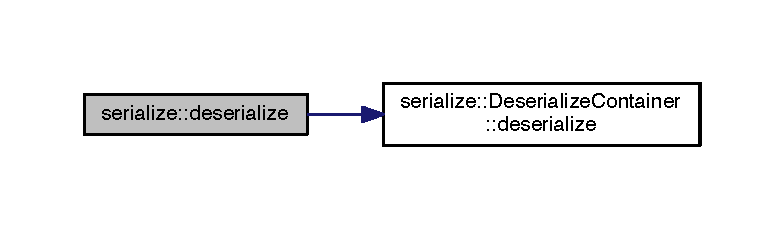
\includegraphics[width=350pt]{namespaceserialize_a4c500beb6e6b8eb1c9e62376d3f5ce83_cgraph}
\end{center}
\end{figure}




Here is the caller graph for this function\+:
\nopagebreak
\begin{figure}[H]
\begin{center}
\leavevmode
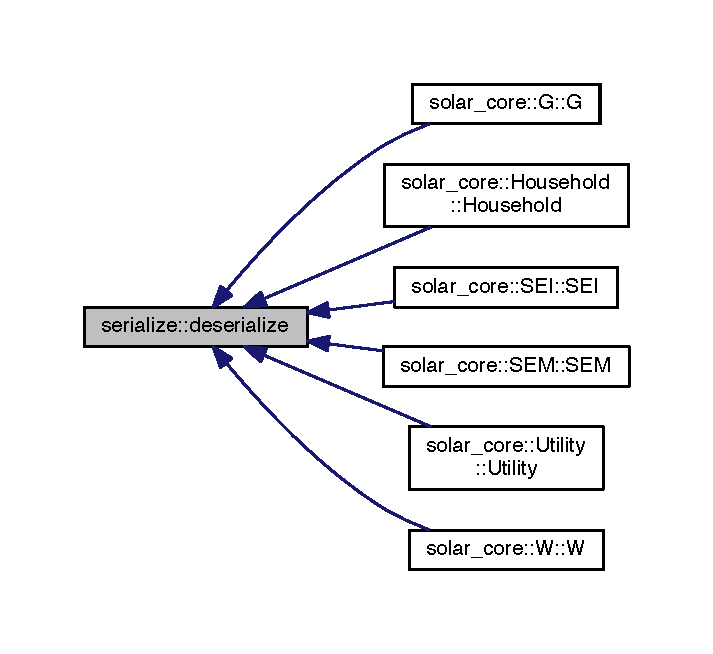
\includegraphics[width=342pt]{namespaceserialize_a4c500beb6e6b8eb1c9e62376d3f5ce83_icgraph}
\end{center}
\end{figure}


\hypertarget{namespaceserialize_a067bdd480e2966e4a61457e64dfbca9e}{}\index{serialize@{serialize}!deserialize@{deserialize}}
\index{deserialize@{deserialize}!serialize@{serialize}}
\subsubsection[{deserialize}]{\setlength{\rightskip}{0pt plus 5cm}template$<$class T $>$ void serialize\+::deserialize (
\begin{DoxyParamCaption}
\item[{const {\bf Property\+Tree} \&}]{pt, }
\item[{std\+::deque$<$ T $>$ \&}]{r}
\end{DoxyParamCaption}
)}\label{namespaceserialize_a067bdd480e2966e4a61457e64dfbca9e}


Definition at line 387 of file Serialize.\+h.



Here is the call graph for this function\+:
\nopagebreak
\begin{figure}[H]
\begin{center}
\leavevmode
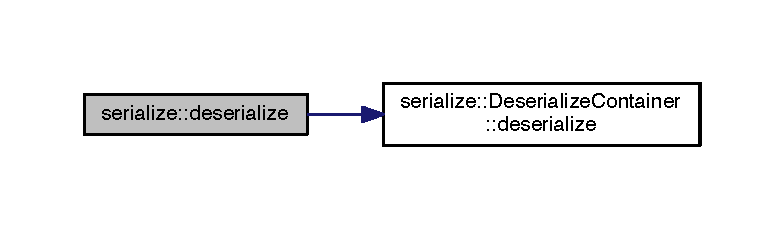
\includegraphics[width=350pt]{namespaceserialize_a067bdd480e2966e4a61457e64dfbca9e_cgraph}
\end{center}
\end{figure}


=======
>>>>>>> 9fadf023062505cb443534457ab9d4d3cc1b7bfc
\hypertarget{namespaceserialize_af7e18cf15b955d078b7fc036042cb083}{}\index{serialize@{serialize}!deserialize@{deserialize}}
\index{deserialize@{deserialize}!serialize@{serialize}}
\subsubsection[{deserialize}]{\setlength{\rightskip}{0pt plus 5cm}template$<$typename K , typename V $>$ void serialize\+::deserialize (
\begin{DoxyParamCaption}
<<<<<<< HEAD
\item[{const {\bf Property\+Tree} \&}]{pt, }
=======
\item[{const Property\+Tree \&}]{pt, }
>>>>>>> 9fadf023062505cb443534457ab9d4d3cc1b7bfc
\item[{std\+::map$<$ K, V $>$ \&}]{r}
\end{DoxyParamCaption}
)}\label{namespaceserialize_af7e18cf15b955d078b7fc036042cb083}
Deserialize into map 

<<<<<<< HEAD
Definition at line 396 of file Serialize.\+h.



Here is the call graph for this function\+:\nopagebreak
=======
Definition at line 169 of file Serialize.\+h.



Here is the call graph for this function\+:
\nopagebreak
>>>>>>> 9fadf023062505cb443534457ab9d4d3cc1b7bfc
\begin{figure}[H]
\begin{center}
\leavevmode
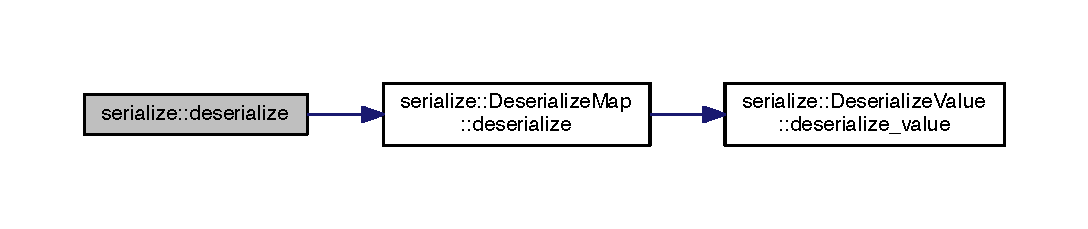
\includegraphics[width=350pt]{namespaceserialize_af7e18cf15b955d078b7fc036042cb083_cgraph}
\end{center}
\end{figure}




Here is the caller graph for this function\+:
\nopagebreak
\begin{figure}[H]
\begin{center}
\leavevmode
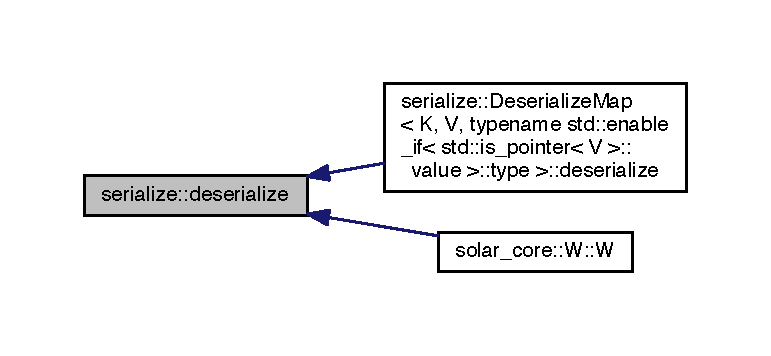
\includegraphics[width=350pt]{namespaceserialize_af7e18cf15b955d078b7fc036042cb083_icgraph}
\end{center}
\end{figure}


\hypertarget{namespaceserialize_ade99c17935e107385ad259ba3111457e}{}\index{serialize@{serialize}!evaluate\+\_\+rpn@{evaluate\+\_\+rpn}}
\index{evaluate\+\_\+rpn@{evaluate\+\_\+rpn}!serialize@{serialize}}
\subsubsection[{evaluate\+\_\+rpn}]{\setlength{\rightskip}{0pt plus 5cm}double serialize\+::evaluate\+\_\+rpn (
\begin{DoxyParamCaption}
\item[{std\+::list$<$ std\+::string $>$ \&}]{tokens}
\end{DoxyParamCaption}
)}\label{namespaceserialize_ade99c17935e107385ad259ba3111457e}
Evaluate R\+P\+N 

<<<<<<< HEAD
Definition at line 185 of file Serialize.\+cpp.



Here is the call graph for this function\+:\nopagebreak
=======
Definition at line 175 of file Serialize.\+cpp.



Here is the call graph for this function\+:
\nopagebreak
>>>>>>> 9fadf023062505cb443534457ab9d4d3cc1b7bfc
\begin{figure}[H]
\begin{center}
\leavevmode
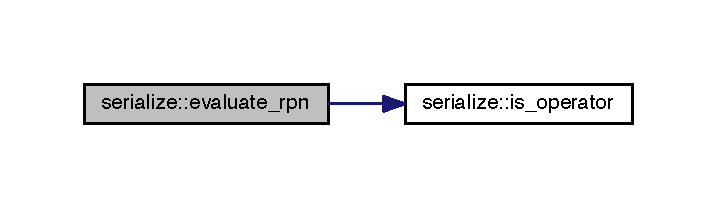
\includegraphics[width=344pt]{namespaceserialize_ade99c17935e107385ad259ba3111457e_cgraph}
\end{center}
\end{figure}




Here is the caller graph for this function\+:
\nopagebreak
\begin{figure}[H]
\begin{center}
\leavevmode
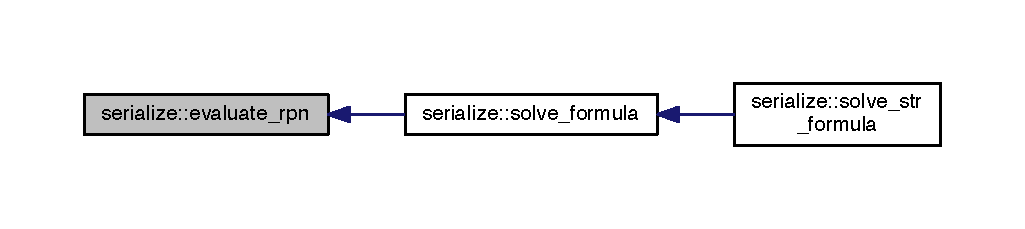
\includegraphics[width=350pt]{namespaceserialize_ade99c17935e107385ad259ba3111457e_icgraph}
\end{center}
\end{figure}


\hypertarget{namespaceserialize_a2876e5d84edeaa969e25a176eb582bb3}{}\index{serialize@{serialize}!infix\+To\+R\+P\+N\+\_\+\+S\+Y\+Alg@{infix\+To\+R\+P\+N\+\_\+\+S\+Y\+Alg}}
\index{infix\+To\+R\+P\+N\+\_\+\+S\+Y\+Alg@{infix\+To\+R\+P\+N\+\_\+\+S\+Y\+Alg}!serialize@{serialize}}
\subsubsection[{infix\+To\+R\+P\+N\+\_\+\+S\+Y\+Alg}]{\setlength{\rightskip}{0pt plus 5cm}std\+::list$<$ std\+::string $>$ serialize\+::infix\+To\+R\+P\+N\+\_\+\+S\+Y\+Alg (
\begin{DoxyParamCaption}
\item[{const std\+::string \&}]{expression\+\_\+}
\end{DoxyParamCaption}
)}\label{namespaceserialize_a2876e5d84edeaa969e25a176eb582bb3}


<<<<<<< HEAD
Definition at line 89 of file Serialize.\+cpp.



Here is the call graph for this function\+:\nopagebreak
=======
Definition at line 81 of file Serialize.\+cpp.



Here is the call graph for this function\+:
\nopagebreak
>>>>>>> 9fadf023062505cb443534457ab9d4d3cc1b7bfc
\begin{figure}[H]
\begin{center}
\leavevmode
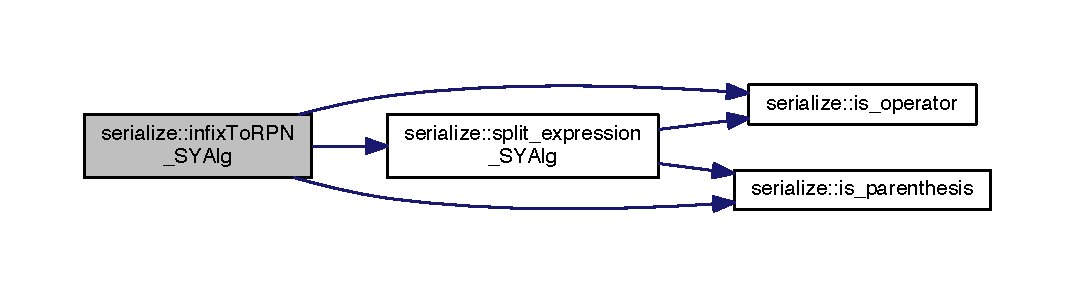
\includegraphics[width=350pt]{namespaceserialize_a2876e5d84edeaa969e25a176eb582bb3_cgraph}
\end{center}
\end{figure}




Here is the caller graph for this function\+:
\nopagebreak
\begin{figure}[H]
\begin{center}
\leavevmode
<<<<<<< HEAD
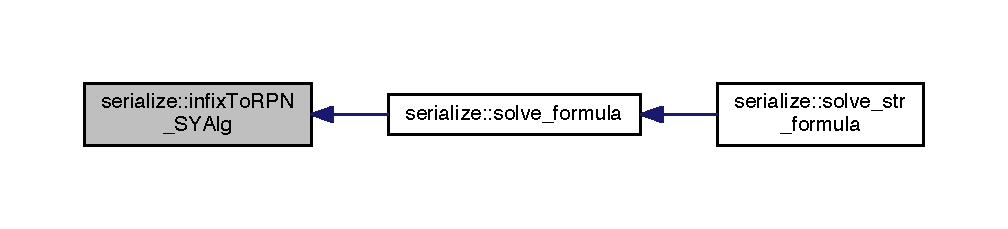
\includegraphics[width=350pt]{namespaceserialize_a2876e5d84edeaa969e25a176eb582bb3_icgraph}
=======
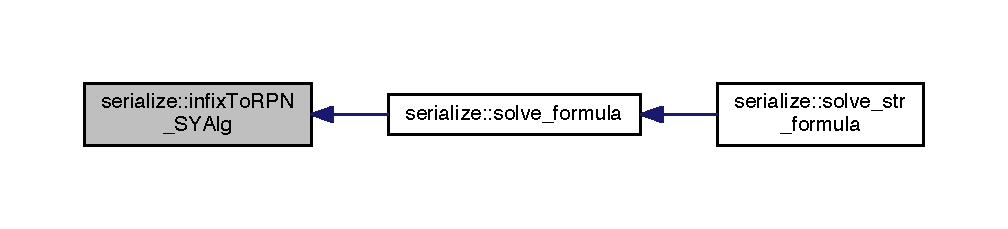
\includegraphics[width=348pt]{namespaceserialize_a2876e5d84edeaa969e25a176eb582bb3_icgraph}
>>>>>>> 9fadf023062505cb443534457ab9d4d3cc1b7bfc
\end{center}
\end{figure}


\hypertarget{namespaceserialize_a897be0f6c9fe37021e11bfeb732d3500}{}\index{serialize@{serialize}!is\+\_\+operator@{is\+\_\+operator}}
\index{is\+\_\+operator@{is\+\_\+operator}!serialize@{serialize}}
\subsubsection[{is\+\_\+operator}]{\setlength{\rightskip}{0pt plus 5cm}bool serialize\+::is\+\_\+operator (
\begin{DoxyParamCaption}
\item[{const std\+::string \&}]{token\+\_\+}
\end{DoxyParamCaption}
)}\label{namespaceserialize_a897be0f6c9fe37021e11bfeb732d3500}


Definition at line 21 of file Serialize.\+cpp.



Here is the caller graph for this function\+:
\nopagebreak
\begin{figure}[H]
\begin{center}
\leavevmode
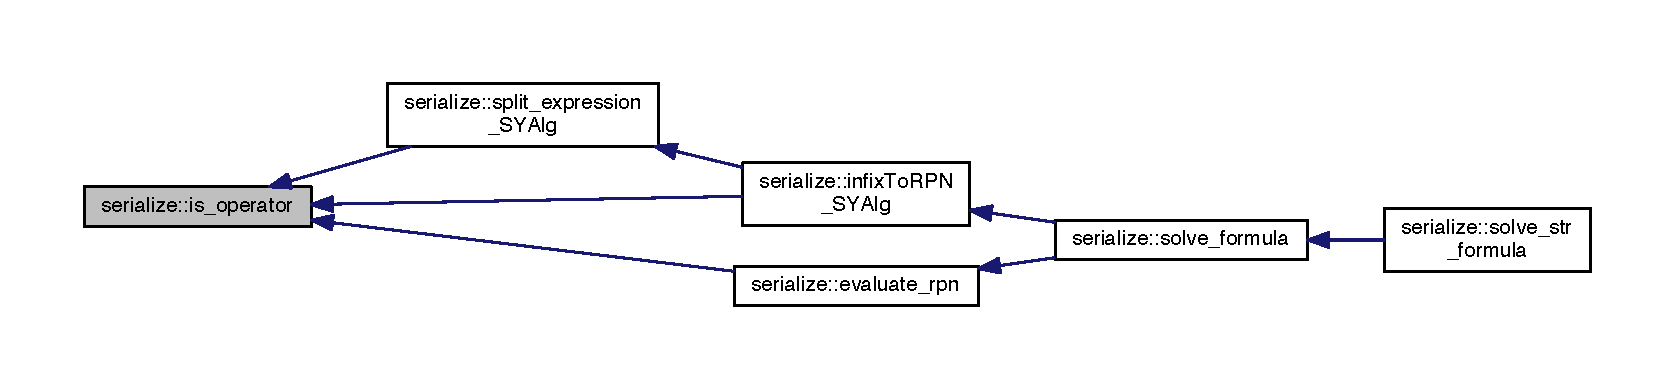
\includegraphics[width=350pt]{namespaceserialize_a897be0f6c9fe37021e11bfeb732d3500_icgraph}
\end{center}
\end{figure}


\hypertarget{namespaceserialize_a38acccd96ada5f0927f924531ac1498e}{}\index{serialize@{serialize}!is\+\_\+parenthesis@{is\+\_\+parenthesis}}
\index{is\+\_\+parenthesis@{is\+\_\+parenthesis}!serialize@{serialize}}
\subsubsection[{is\+\_\+parenthesis}]{\setlength{\rightskip}{0pt plus 5cm}bool serialize\+::is\+\_\+parenthesis (
\begin{DoxyParamCaption}
\item[{const std\+::string \&}]{token\+\_\+}
\end{DoxyParamCaption}
)}\label{namespaceserialize_a38acccd96ada5f0927f924531ac1498e}


Definition at line 14 of file Serialize.\+cpp.



Here is the caller graph for this function\+:
\nopagebreak
\begin{figure}[H]
\begin{center}
\leavevmode
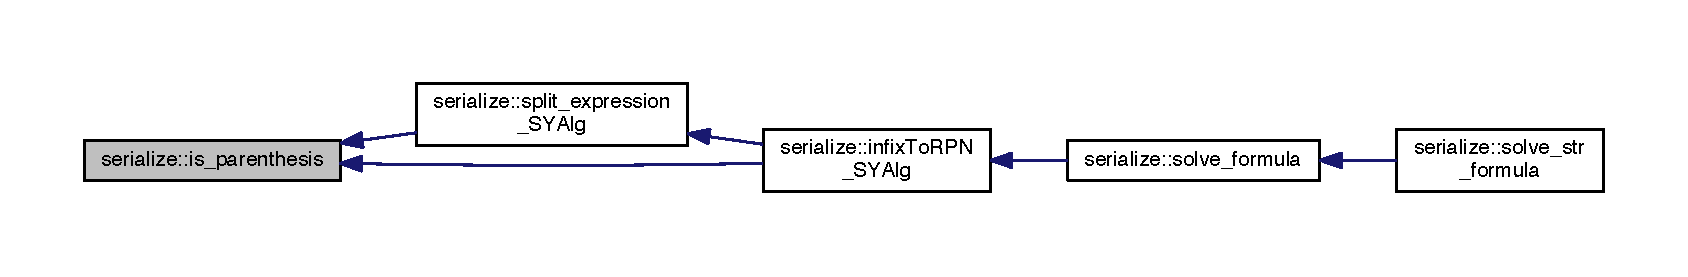
\includegraphics[width=350pt]{namespaceserialize_a38acccd96ada5f0927f924531ac1498e_icgraph}
\end{center}
\end{figure}


<<<<<<< HEAD
\hypertarget{namespaceserialize_a48d3582d3d99189f6f067e77d962574f}{}\index{serialize@{serialize}!serialize@{serialize}}
\index{serialize@{serialize}!serialize@{serialize}}
\subsubsection[{serialize}]{\setlength{\rightskip}{0pt plus 5cm}template$<$class T $>$ {\bf Property\+Tree} serialize\+::serialize (
\begin{DoxyParamCaption}
\item[{std\+::vector$<$ T $>$ \&}]{container\+\_\+, }
\item[{Property\+Tree\+::key\+\_\+type const \&}]{key}
\end{DoxyParamCaption}
)}\label{namespaceserialize_a48d3582d3d99189f6f067e77d962574f}
Wrapper for call to serialize vector, deque, map. Does not change. 

Definition at line 198 of file Serialize.\+h.



Here is the call graph for this function\+:
\nopagebreak
\begin{figure}[H]
\begin{center}
\leavevmode
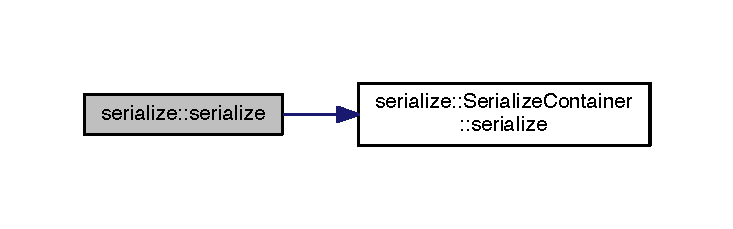
\includegraphics[width=350pt]{namespaceserialize_a48d3582d3d99189f6f067e77d962574f_cgraph}
\end{center}
\end{figure}




Here is the caller graph for this function\+:
\nopagebreak
\begin{figure}[H]
\begin{center}
\leavevmode
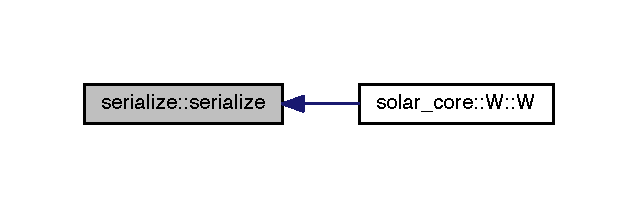
\includegraphics[width=306pt]{namespaceserialize_a48d3582d3d99189f6f067e77d962574f_icgraph}
\end{center}
\end{figure}


\hypertarget{namespaceserialize_aa60e366236e42c68f437ea409aa0e056}{}\index{serialize@{serialize}!serialize@{serialize}}
\index{serialize@{serialize}!serialize@{serialize}}
\subsubsection[{serialize}]{\setlength{\rightskip}{0pt plus 5cm}template$<$class T $>$ {\bf Property\+Tree} serialize\+::serialize (
\begin{DoxyParamCaption}
\item[{std\+::deque$<$ T $>$ \&}]{container\+\_\+, }
\item[{Property\+Tree\+::key\+\_\+type const \&}]{key}
\end{DoxyParamCaption}
)}\label{namespaceserialize_aa60e366236e42c68f437ea409aa0e056}


Definition at line 201 of file Serialize.\+h.



Here is the call graph for this function\+:
\nopagebreak
\begin{figure}[H]
\begin{center}
\leavevmode
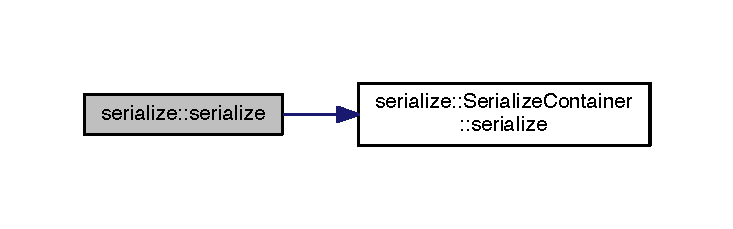
\includegraphics[width=350pt]{namespaceserialize_aa60e366236e42c68f437ea409aa0e056_cgraph}
\end{center}
\end{figure}


\hypertarget{namespaceserialize_a585cc862a49aec3bc1deca353af0b53c}{}\index{serialize@{serialize}!serialize@{serialize}}
\index{serialize@{serialize}!serialize@{serialize}}
\subsubsection[{serialize}]{\setlength{\rightskip}{0pt plus 5cm}template$<$typename K , typename V $>$ {\bf Property\+Tree} serialize\+::serialize (
\begin{DoxyParamCaption}
\item[{std\+::map$<$ K, V $>$ \&}]{container\+\_\+, }
\item[{Property\+Tree\+::key\+\_\+type const \&}]{key}
\end{DoxyParamCaption}
)}\label{namespaceserialize_a585cc862a49aec3bc1deca353af0b53c}


Definition at line 204 of file Serialize.\+h.



Here is the call graph for this function\+:
\nopagebreak
\begin{figure}[H]
\begin{center}
\leavevmode
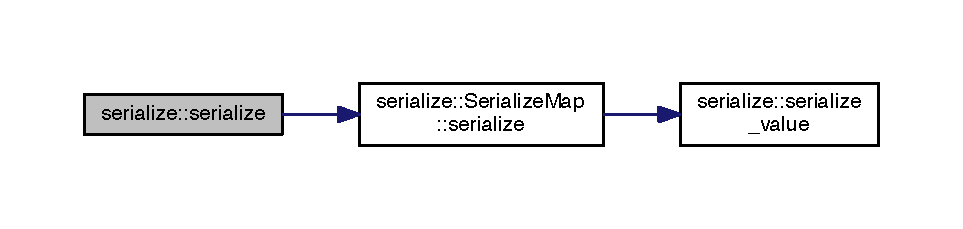
\includegraphics[width=350pt]{namespaceserialize_a585cc862a49aec3bc1deca353af0b53c_cgraph}
\end{center}
\end{figure}


\hypertarget{namespaceserialize_afcd8d07d106f4bf71ce8813e6c2ccbd8}{}\index{serialize@{serialize}!serialize\+\_\+value@{serialize\+\_\+value}}
\index{serialize\+\_\+value@{serialize\+\_\+value}!serialize@{serialize}}
\subsubsection[{serialize\+\_\+value}]{\setlength{\rightskip}{0pt plus 5cm}template$<$typename In $>$ void serialize\+::serialize\+\_\+value (
\begin{DoxyParamCaption}
\item[{In \&}]{in\+\_\+, }
\item[{std\+::string \&}]{out\+\_\+}
\end{DoxyParamCaption}
)}\label{namespaceserialize_afcd8d07d106f4bf71ce8813e6c2ccbd8}
Service function for serialization through string stream. 

Definition at line 48 of file Serialize.\+h.



Here is the caller graph for this function\+:
\nopagebreak
\begin{figure}[H]
\begin{center}
\leavevmode
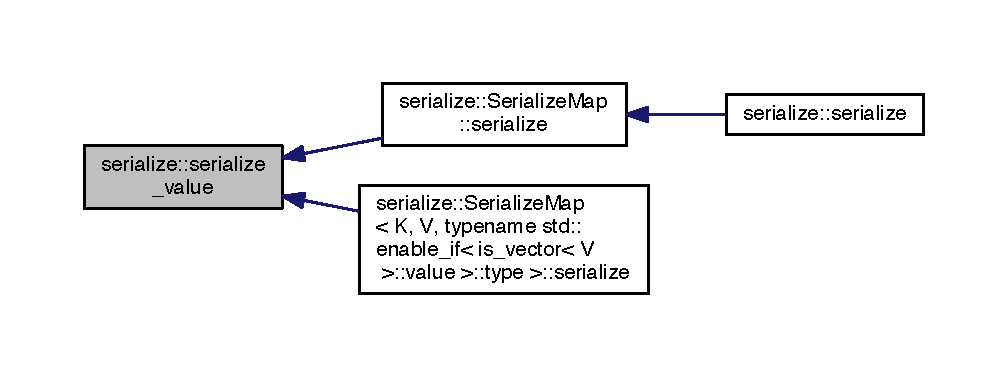
\includegraphics[width=350pt]{namespaceserialize_afcd8d07d106f4bf71ce8813e6c2ccbd8_icgraph}
\end{center}
\end{figure}


=======
>>>>>>> 9fadf023062505cb443534457ab9d4d3cc1b7bfc
\hypertarget{namespaceserialize_a8efbe7c32352f8ff750211235e3d5361}{}\index{serialize@{serialize}!solve\+\_\+formula@{solve\+\_\+formula}}
\index{solve\+\_\+formula@{solve\+\_\+formula}!serialize@{serialize}}
\subsubsection[{solve\+\_\+formula}]{\setlength{\rightskip}{0pt plus 5cm}double serialize\+::solve\+\_\+formula (
\begin{DoxyParamCaption}
\item[{std\+::string}]{str\+\_\+}
\end{DoxyParamCaption}
)}\label{namespaceserialize_a8efbe7c32352f8ff750211235e3d5361}
Simple algorithm to solve mathematical formulas 

<<<<<<< HEAD
Definition at line 242 of file Serialize.\+cpp.



Here is the call graph for this function\+:\nopagebreak
\begin{figure}[H]
\begin{center}
\leavevmode
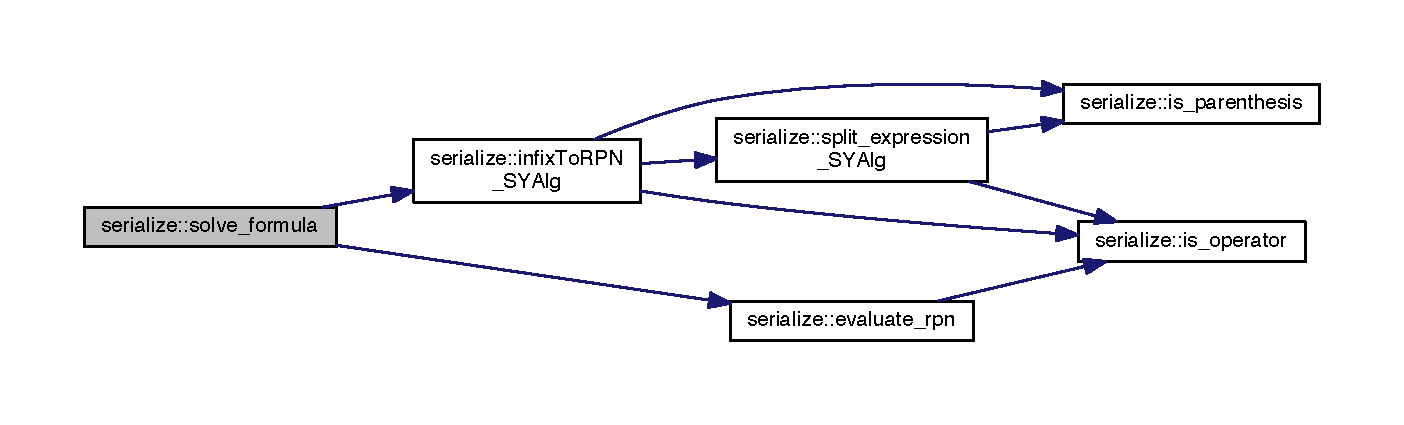
\includegraphics[width=350pt]{namespaceserialize_a8efbe7c32352f8ff750211235e3d5361_cgraph}
\end{center}
\end{figure}




Here is the caller graph for this function\+:
=======
Definition at line 233 of file Serialize.\+cpp.



Here is the call graph for this function\+:
>>>>>>> 9fadf023062505cb443534457ab9d4d3cc1b7bfc
\nopagebreak
\begin{figure}[H]
\begin{center}
\leavevmode
<<<<<<< HEAD
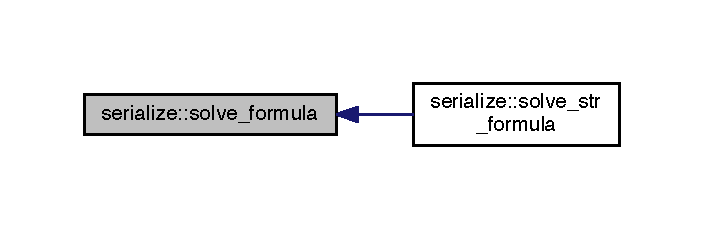
\includegraphics[width=338pt]{namespaceserialize_a8efbe7c32352f8ff750211235e3d5361_icgraph}
=======
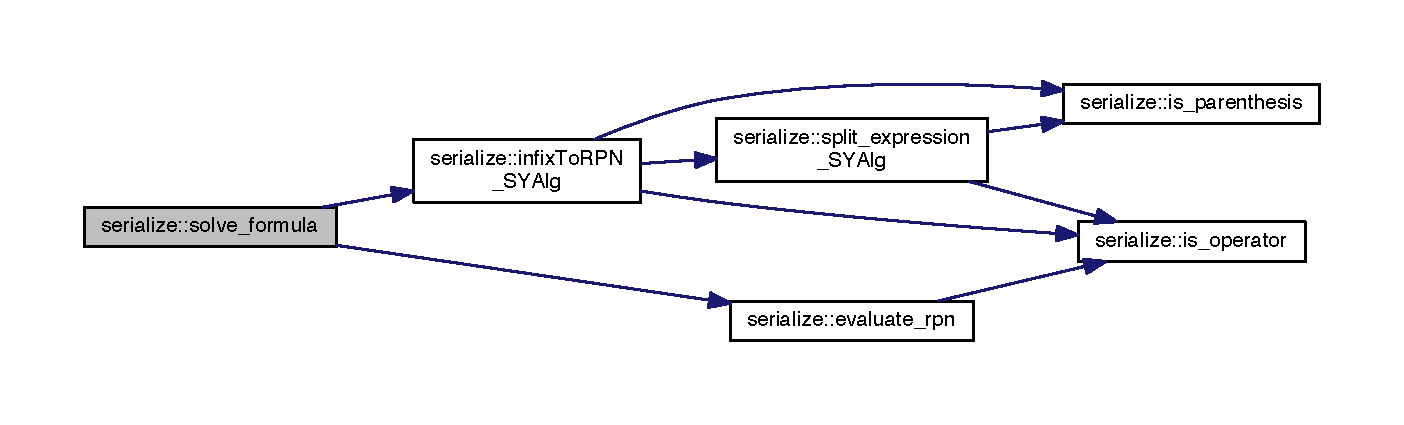
\includegraphics[width=350pt]{namespaceserialize_a8efbe7c32352f8ff750211235e3d5361_cgraph}
>>>>>>> 9fadf023062505cb443534457ab9d4d3cc1b7bfc
\end{center}
\end{figure}


<<<<<<< HEAD
\hypertarget{namespaceserialize_aa5ee0bad0c960a3f06430066217d8c12}{}\index{serialize@{serialize}!solve\+\_\+str\+\_\+formula@{solve\+\_\+str\+\_\+formula}}
\index{solve\+\_\+str\+\_\+formula@{solve\+\_\+str\+\_\+formula}!serialize@{serialize}}
\subsubsection[{solve\+\_\+str\+\_\+formula}]{\setlength{\rightskip}{0pt plus 5cm}template$<$class T $>$ T serialize\+::solve\+\_\+str\+\_\+formula (
\begin{DoxyParamCaption}
\item[{const std\+::string \&}]{formula\+\_\+, }
\item[{{\bf I\+Random} \&}]{rand\+\_\+}
\end{DoxyParamCaption}
)}\label{namespaceserialize_aa5ee0bad0c960a3f06430066217d8c12}
M\+A\+R\+K\+: cont. \begin{DoxyRefDesc}{Dev\+Stage2}
\item[\hyperlink{_dev_stage2__DevStage2000027}{Dev\+Stage2}]change to better Truncated generation \end{DoxyRefDesc}


careful here -\/ will find both u and u\+\_\+int 

Definition at line 453 of file Serialize.\+h.



Here is the call graph for this function\+:
\nopagebreak
\begin{figure}[H]
\begin{center}
\leavevmode
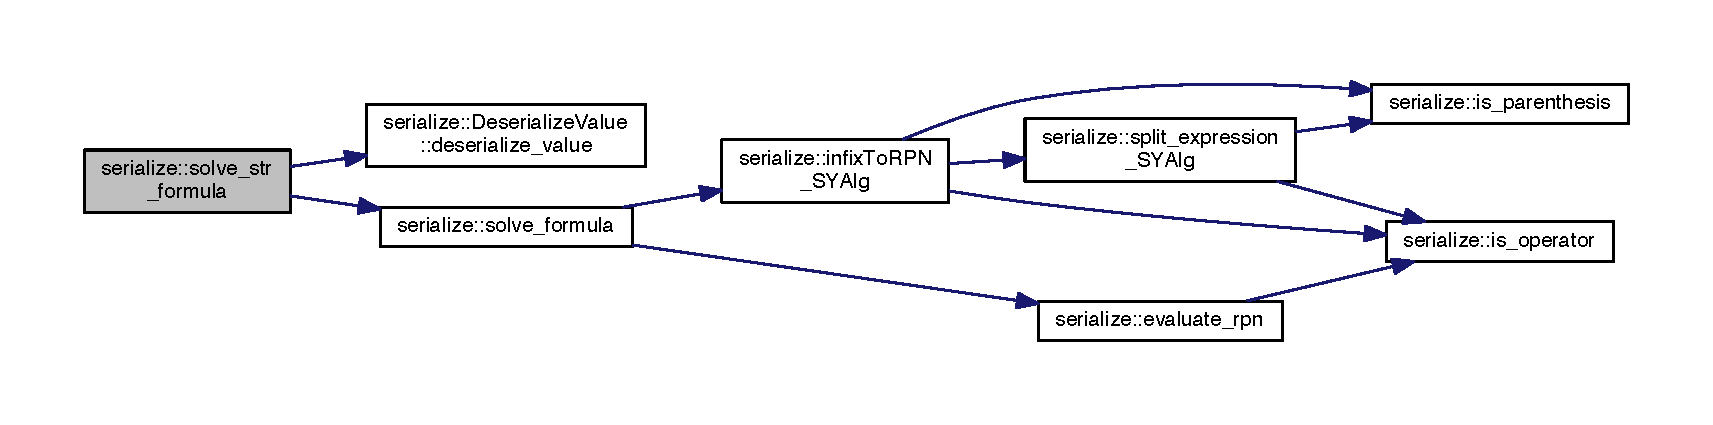
\includegraphics[width=350pt]{namespaceserialize_aa5ee0bad0c960a3f06430066217d8c12_cgraph}
\end{center}
\end{figure}

=======
\hypertarget{namespaceserialize_a2c1ea7730402ca3407bced2235efe3fd}{}\index{serialize@{serialize}!solve\+\_\+str\+\_\+formula@{solve\+\_\+str\+\_\+formula}}
\index{solve\+\_\+str\+\_\+formula@{solve\+\_\+str\+\_\+formula}!serialize@{serialize}}
\subsubsection[{solve\+\_\+str\+\_\+formula}]{\setlength{\rightskip}{0pt plus 5cm}template$<$class $>$ void serialize\+::solve\+\_\+str\+\_\+formula (
\begin{DoxyParamCaption}
\item[{std\+::string \&}]{formula\+\_\+}
\end{DoxyParamCaption}
)}\label{namespaceserialize_a2c1ea7730402ca3407bced2235efe3fd}
M\+A\+R\+K\+: cont. 

Definition at line 226 of file Serialize.\+h.
>>>>>>> 9fadf023062505cb443534457ab9d4d3cc1b7bfc

\hypertarget{namespaceserialize_a06d144912d025816fe84c532295d274a}{}\index{serialize@{serialize}!split\+\_\+expression\+\_\+\+S\+Y\+Alg@{split\+\_\+expression\+\_\+\+S\+Y\+Alg}}
\index{split\+\_\+expression\+\_\+\+S\+Y\+Alg@{split\+\_\+expression\+\_\+\+S\+Y\+Alg}!serialize@{serialize}}
\subsubsection[{split\+\_\+expression\+\_\+\+S\+Y\+Alg}]{\setlength{\rightskip}{0pt plus 5cm}std\+::vector$<$ std\+::string $>$ serialize\+::split\+\_\+expression\+\_\+\+S\+Y\+Alg (
\begin{DoxyParamCaption}
\item[{const std\+::string \&}]{expression\+\_\+}
\end{DoxyParamCaption}
)}\label{namespaceserialize_a06d144912d025816fe84c532295d274a}


Definition at line 31 of file Serialize.\+cpp.



<<<<<<< HEAD
Here is the call graph for this function\+:\nopagebreak
=======
Here is the call graph for this function\+:
\nopagebreak
>>>>>>> 9fadf023062505cb443534457ab9d4d3cc1b7bfc
\begin{figure}[H]
\begin{center}
\leavevmode
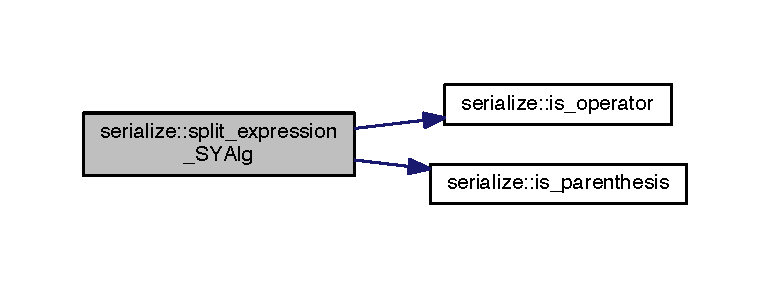
\includegraphics[width=350pt]{namespaceserialize_a06d144912d025816fe84c532295d274a_cgraph}
\end{center}
\end{figure}




Here is the caller graph for this function\+:
\nopagebreak
\begin{figure}[H]
\begin{center}
\leavevmode
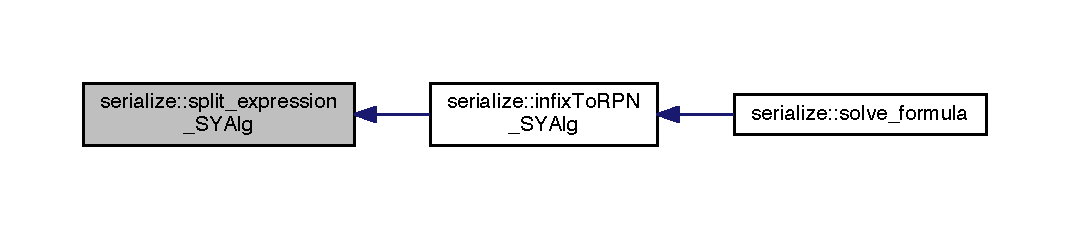
\includegraphics[width=350pt]{namespaceserialize_a06d144912d025816fe84c532295d274a_icgraph}
\end{center}
\end{figure}



\hypertarget{namespacesolar__core}{}\section{solar\+\_\+core Namespace Reference}
\label{namespacesolar__core}\index{solar\+\_\+core@{solar\+\_\+core}}
\subsection*{Namespaces}
\begin{DoxyCompactItemize}
\item 
 \hyperlink{namespacesolar__core_1_1constants}{constants}
\end{DoxyCompactItemize}
\subsection*{Classes}
\begin{DoxyCompactItemize}
\item 
class \hyperlink{classsolar__core_1_1_g}{G}
\item 
class \hyperlink{classsolar__core_1_1_house}{House}
\item 
class \hyperlink{classsolar__core_1_1_household}{Household}
\item 
class \hyperlink{classsolar__core_1_1_i_agent}{I\+Agent}
\item 
class \hyperlink{classsolar__core_1_1_i_institute}{I\+Institute}
\item 
class \hyperlink{classsolar__core_1_1_marketing_inst}{Marketing\+Inst}
\item 
class \hyperlink{classsolar__core_1_1_mes_design}{Mes\+Design}
\item 
class \hyperlink{classsolar__core_1_1_mes_finance}{Mes\+Finance}
\item 
class \hyperlink{classsolar__core_1_1_mes_marketing_s_e_i}{Mes\+Marketing\+S\+E\+I}
\item 
class \hyperlink{classsolar__core_1_1_mes_marketing_s_e_i_online_quote}{Mes\+Marketing\+S\+E\+I\+Online\+Quote}
\item 
class \hyperlink{classsolar__core_1_1_mes_marketing_s_e_i_preliminary_quote}{Mes\+Marketing\+S\+E\+I\+Preliminary\+Quote}
\item 
class \hyperlink{classsolar__core_1_1_mes_payment}{Mes\+Payment}
\item 
class \hyperlink{classsolar__core_1_1_mes_state_base_h_h}{Mes\+State\+Base\+H\+H}
\item 
class \hyperlink{classsolar__core_1_1_p_v_design}{P\+V\+Design}
\item 
class \hyperlink{classsolar__core_1_1_p_v_project}{P\+V\+Project}
\item 
class \hyperlink{classsolar__core_1_1_s_e_i}{S\+E\+I}
\item 
class \hyperlink{classsolar__core_1_1_solar_module}{Solar\+Module}
\item 
class \hyperlink{classsolar__core_1_1_tile}{Tile}
\item 
class \hyperlink{classsolar__core_1_1_w}{W}
\item 
class \hyperlink{classsolar__core_1_1_world_map}{World\+Map}
\item 
class \hyperlink{classsolar__core_1_1_world_settings}{World\+Settings}
\end{DoxyCompactItemize}
\subsection*{Typedefs}
\begin{DoxyCompactItemize}
\item 
typedef int64\+\_\+t \hyperlink{namespacesolar__core_a4b5949d07259da6f8a20d12a30403e90}{Time\+Unit}
\item 
typedef boost\+::property\+\_\+tree\+::ptree \hyperlink{namespacesolar__core_adeda2737d6938c190eb774a5b2495045}{Property\+Tree}
\item 
typedef std\+::underlying\+\_\+type$<$ \hyperlink{namespacesolar__core_aa1147341e5ef7a40d68d1bd68e149362}{E\+Param\+Types} $>$\+::type \hyperlink{namespacesolar__core_a256e8e2dc052f522b522d3f90b294caf}{E\+Param\+Types\+\_\+type}
\end{DoxyCompactItemize}
\subsection*{Enumerations}
\begin{DoxyCompactItemize}
\item 
enum \hyperlink{namespacesolar__core_aa1147341e5ef7a40d68d1bd68e149362}{E\+Param\+Types} \+: int64\+\_\+t \{ \\*
\hyperlink{namespacesolar__core_aa1147341e5ef7a40d68d1bd68e149362a1f08d08fd864b99cbeebd88b9a0784a7}{E\+Param\+Types\+::\+Income}, 
\hyperlink{namespacesolar__core_aa1147341e5ef7a40d68d1bd68e149362a62c5cc90270449db38e6fb4f2db71c55}{E\+Param\+Types\+::\+N\+\_\+\+H}, 
\hyperlink{namespacesolar__core_aa1147341e5ef7a40d68d1bd68e149362a417bef7b89fce8abf638b9983a79a70e}{E\+Param\+Types\+::\+Credit\+Score}, 
\hyperlink{namespacesolar__core_aa1147341e5ef7a40d68d1bd68e149362a9b8cd62150c419c61129f736404b0579}{E\+Param\+Types\+::\+Electricity\+Bill}, 
\\*
\hyperlink{namespacesolar__core_aa1147341e5ef7a40d68d1bd68e149362a2bf6593af19bb602f7c596d7327c6dd6}{E\+Param\+Types\+::\+Roof\+Size}, 
\hyperlink{namespacesolar__core_aa1147341e5ef7a40d68d1bd68e149362abff61b25127aa53b8eb7343edf48166b}{E\+Param\+Types\+::\+Roof\+Age}, 
\hyperlink{namespacesolar__core_aa1147341e5ef7a40d68d1bd68e149362afc91168d2e624505b0168a1ee8c0c60e}{E\+Param\+Types\+::\+H\+H\+Marketing\+State\+Highly\+Interested}, 
\hyperlink{namespacesolar__core_aa1147341e5ef7a40d68d1bd68e149362a985f6ff4deb35454155c9e992bfcdbb0}{E\+Param\+Types\+::\+H\+H\+Marketing\+State\+Interested}, 
\\*
\hyperlink{namespacesolar__core_aa1147341e5ef7a40d68d1bd68e149362ab970e992ff02930a86716c0390fa42df}{E\+Param\+Types\+::\+H\+H\+Marketing\+Not\+Interested}, 
\hyperlink{namespacesolar__core_aa1147341e5ef7a40d68d1bd68e149362a5a8012f218ced859bad78be09e8e46e7}{E\+Param\+Types\+::\+Active\+Quoting}, 
\hyperlink{namespacesolar__core_aa1147341e5ef7a40d68d1bd68e149362a31ead751600c8439e0897f8dc736154b}{E\+Param\+Types\+::\+Inactive\+Quoting}, 
\hyperlink{namespacesolar__core_aa1147341e5ef7a40d68d1bd68e149362a374a1855dae7569f1de9514f0cdf09f5}{E\+Param\+Types\+::\+H\+H\+Decision\+Reroof}, 
\\*
\hyperlink{namespacesolar__core_aa1147341e5ef7a40d68d1bd68e149362a4580119737f0c25977ece80cbac3d58b}{E\+Param\+Types\+::\+H\+H\+Max\+N\+Visits\+Per\+Time\+Unit}, 
\hyperlink{namespacesolar__core_aa1147341e5ef7a40d68d1bd68e149362a619c634adba7a1386122c22d8d2021df}{E\+Param\+Types\+::\+H\+H\+Dec\+Preliminary\+Quote}, 
\hyperlink{namespacesolar__core_aa1147341e5ef7a40d68d1bd68e149362a91a0e5bcf4376200527bfe2b00d1ae6c}{E\+Param\+Types\+::\+Requested\+Online\+Quote}, 
\hyperlink{namespacesolar__core_aa1147341e5ef7a40d68d1bd68e149362a6d84e672f96624f4c6323a7543a5de1f}{E\+Param\+Types\+::\+Request\+Preliminary\+Quote}, 
\\*
\hyperlink{namespacesolar__core_aa1147341e5ef7a40d68d1bd68e149362a3f1645b895f679824026ca1de865ca81}{E\+Param\+Types\+::\+Requested\+Preliminary\+Quote}, 
\hyperlink{namespacesolar__core_aa1147341e5ef7a40d68d1bd68e149362a5d1561cc7b77d4e0eaca8cc37a4331e9}{E\+Param\+Types\+::\+Provided\+Online\+Quote}, 
\hyperlink{namespacesolar__core_aa1147341e5ef7a40d68d1bd68e149362ac3d9027c79b1821115c110ce9b706383}{E\+Param\+Types\+::\+Provided\+Preliminary\+Quote}, 
\hyperlink{namespacesolar__core_aa1147341e5ef7a40d68d1bd68e149362a6f85c2280e06a0a94e796e2c6dfbfce2}{E\+Param\+Types\+::\+Scheduled\+First\+Site\+Visit}, 
\\*
\hyperlink{namespacesolar__core_aa1147341e5ef7a40d68d1bd68e149362a1944aa6a68e41524b170bb07ba22fb54}{E\+Param\+Types\+::\+Collected\+Inf\+First\+Site\+Visit}, 
\hyperlink{namespacesolar__core_aa1147341e5ef7a40d68d1bd68e149362a94beae8137095b64c636645a10f779a9}{E\+Param\+Types\+::\+Required\+H\+H\+Reroof}, 
\hyperlink{namespacesolar__core_aa1147341e5ef7a40d68d1bd68e149362a7a0186947edeb230395b02fc6f9a8c37}{E\+Param\+Types\+::\+Waiting\+H\+H\+Reroof}, 
\hyperlink{namespacesolar__core_aa1147341e5ef7a40d68d1bd68e149362ae04bb6f7c490d1f5e1e19b790ac4bd48}{E\+Param\+Types\+::\+Accepted\+Preliminary\+Quote}, 
\\*
\hyperlink{namespacesolar__core_aa1147341e5ef7a40d68d1bd68e149362a8662266053d427b356392cc9fdff7b5e}{E\+Param\+Types\+::\+Drafted\+Design}, 
\hyperlink{namespacesolar__core_aa1147341e5ef7a40d68d1bd68e149362acc5c79b9e52a3187a8b3bfdf7796f6e5}{E\+Param\+Types\+::\+Accepted\+Design}, 
\hyperlink{namespacesolar__core_aa1147341e5ef7a40d68d1bd68e149362aca58ef2d2dad5072c87d596308db83d0}{E\+Param\+Types\+::\+Requested\+Permit}, 
\hyperlink{namespacesolar__core_aa1147341e5ef7a40d68d1bd68e149362a9a4ff00bed0dd4c2cbcd986eb71654b5}{E\+Param\+Types\+::\+Granted\+Permit}, 
\\*
\hyperlink{namespacesolar__core_aa1147341e5ef7a40d68d1bd68e149362a1246349928f17a03f4bc9fc73929013a}{E\+Param\+Types\+::\+Scheduled\+Installation}, 
\hyperlink{namespacesolar__core_aa1147341e5ef7a40d68d1bd68e149362a98dd43dfae05b11befe1f140e0ec787a}{E\+Param\+Types\+::\+Installed}, 
\hyperlink{namespacesolar__core_aa1147341e5ef7a40d68d1bd68e149362a36011ab25e125345f76caf5e8f027175}{E\+Param\+Types\+::\+Closed\+Project}, 
\hyperlink{namespacesolar__core_aa1147341e5ef7a40d68d1bd68e149362ac2c46b3ff478ae34297f8672b3d91497}{E\+Param\+Types\+::\+Online\+Quote\+Price}, 
\\*
\hyperlink{namespacesolar__core_aa1147341e5ef7a40d68d1bd68e149362a9cdd993b8d48601635f529f0e4d93299}{E\+Param\+Types\+::\+Online\+Quote\+Estimated\+Savings}, 
\hyperlink{namespacesolar__core_aa1147341e5ef7a40d68d1bd68e149362a581329dc30b846b1b05267c8bbfb3dc2}{E\+Param\+Types\+::\+Preliminary\+Quote\+Price}, 
\hyperlink{namespacesolar__core_aa1147341e5ef7a40d68d1bd68e149362ac9882efbffdf2ae9422abfc3e4d4a032}{E\+Param\+Types\+::\+Preliminary\+Quote\+Estimated\+Savings}, 
\hyperlink{namespacesolar__core_aa1147341e5ef7a40d68d1bd68e149362a65e9babf589ac04a35221b97b0449611}{E\+Param\+Types\+::\+Estimated\+Price\+Per\+Watt}, 
\\*
\hyperlink{namespacesolar__core_aa1147341e5ef7a40d68d1bd68e149362a00420d47e5664414646cd5cc5245c914}{E\+Param\+Types\+::\+Average\+P\+V\+Price}, 
\hyperlink{namespacesolar__core_aa1147341e5ef7a40d68d1bd68e149362ab820b21cf6b896d9ffe4f3180344aaad}{E\+Param\+Types\+::\+Average\+P\+V\+Capacity}, 
\hyperlink{namespacesolar__core_aa1147341e5ef7a40d68d1bd68e149362a95318d634060f210ca2cbc8487913a23}{E\+Param\+Types\+::\+Electricity\+Price\+U\+C\+Demand}, 
\hyperlink{namespacesolar__core_aa1147341e5ef7a40d68d1bd68e149362a57bd39ffa6aea05e5ffe8481417466f8}{E\+Param\+Types\+::\+Electricity\+Price\+U\+C\+Supply}, 
\\*
\hyperlink{namespacesolar__core_aa1147341e5ef7a40d68d1bd68e149362a7f416fbc5b5a75a37caa766533274218}{E\+Param\+Types\+::\+Inflation\+Rate}, 
\hyperlink{namespacesolar__core_aa1147341e5ef7a40d68d1bd68e149362ab49cdbc17a92df4982fae394c33aac83}{E\+Param\+Types\+::\+D\+Cto\+A\+C\+Loss}, 
\hyperlink{namespacesolar__core_aa1147341e5ef7a40d68d1bd68e149362a2b772976cb89ca861f4a970d8eed2959}{E\+Param\+Types\+::\+S\+E\+I\+Small}, 
\hyperlink{namespacesolar__core_aa1147341e5ef7a40d68d1bd68e149362a827914969a84c51a2e5722d05a311c97}{E\+Param\+Types\+::\+S\+E\+I\+Large}, 
\\*
\hyperlink{namespacesolar__core_aa1147341e5ef7a40d68d1bd68e149362a159b446def618d2defa97ad1818ad6dc}{E\+Param\+Types\+::\+S\+E\+I\+Processing\+Time\+Required\+For\+Preliminary\+Quote}, 
\hyperlink{namespacesolar__core_aa1147341e5ef7a40d68d1bd68e149362aee8260c2afdde8270a04e738d6dfd61e}{E\+Param\+Types\+::\+S\+E\+I\+Processing\+Time\+Required\+For\+Scheduling\+First\+Site\+Visit}, 
\hyperlink{namespacesolar__core_aa1147341e5ef7a40d68d1bd68e149362a21df8a580ed978b021e23a928d19b29e}{E\+Param\+Types\+::\+S\+E\+I\+Processing\+Time\+Required\+For\+Design}, 
\hyperlink{namespacesolar__core_aa1147341e5ef7a40d68d1bd68e149362ad6e334fa57e5846cf4ba4b182dadca1d}{E\+Param\+Types\+::\+S\+E\+I\+Max\+N\+Visits\+Per\+Time\+Unit}, 
\\*
\hyperlink{namespacesolar__core_aa1147341e5ef7a40d68d1bd68e149362acd42418f4ce0736c05d2aa8b36694774}{E\+Param\+Types\+::\+S\+E\+I\+Max\+N\+Installations\+Per\+Time\+Unit}, 
\hyperlink{namespacesolar__core_aa1147341e5ef7a40d68d1bd68e149362a79d36b9c925b7e55309fd4436f67c4ee}{E\+Param\+Types\+::\+S\+E\+I\+Max\+Roof\+Age}, 
\hyperlink{namespacesolar__core_aa1147341e5ef7a40d68d1bd68e149362ae48d553d39bcd7d207890c610fa1e74c}{E\+Param\+Types\+::\+S\+E\+I\+Frequency\+Update\+Design\+Templates}, 
\hyperlink{namespacesolar__core_aa1147341e5ef7a40d68d1bd68e149362ad03dae753c26cb012acd3a7dcd41dc8c}{E\+Param\+Types\+::\+S\+E\+I\+High\+Efficiency\+Design}, 
\\*
\hyperlink{namespacesolar__core_aa1147341e5ef7a40d68d1bd68e149362a2b4390775acd3d31e3049d242a1dd196}{E\+Param\+Types\+::\+S\+E\+I\+Mid\+Efficiency\+Design}, 
\hyperlink{namespacesolar__core_aa1147341e5ef7a40d68d1bd68e149362ab2592ca389b1a29cf91ddefe8d6769a2}{E\+Param\+Types\+::\+S\+E\+I\+Low\+Efficiency\+Design}, 
\hyperlink{namespacesolar__core_aa1147341e5ef7a40d68d1bd68e149362a7863d48ef49981916e8a483f2171b306}{E\+Param\+Types\+::\+Payments\+On\+Time}, 
\hyperlink{namespacesolar__core_aa1147341e5ef7a40d68d1bd68e149362a6adf97f83acf6453d4a6a4b1070f3754}{E\+Param\+Types\+::\+None}
 \}
\item 
enum \hyperlink{namespacesolar__core_ac827fdef4412a3c0d5e44d3f31908e49}{E\+Constraint\+Params} \+: int64\+\_\+t \{ \\*
\hyperlink{namespacesolar__core_ac827fdef4412a3c0d5e44d3f31908e49a79b059203dc39b55d85046f355d1fa95}{E\+Constraint\+Params\+::\+Max\+N\+Ticks\+To\+Collect\+Quotes}, 
\hyperlink{namespacesolar__core_ac827fdef4412a3c0d5e44d3f31908e49a5d0891420ec7c6769c9ece305c98daac}{E\+Constraint\+Params\+::\+Max\+N\+Open\+Projects\+H\+H}, 
\hyperlink{namespacesolar__core_ac827fdef4412a3c0d5e44d3f31908e49ae497930a8f22e14387bac31ebe737a64}{E\+Constraint\+Params\+::\+Max\+N\+Requested\+Preliminary\+From\+Online\+Quotes}, 
\hyperlink{namespacesolar__core_ac827fdef4412a3c0d5e44d3f31908e49a2e66c9bd577b41e92fd40c619a886559}{E\+Constraint\+Params\+::\+Min\+N\+Received\+Preliminary\+Quotes}, 
\\*
\hyperlink{namespacesolar__core_ac827fdef4412a3c0d5e44d3f31908e49a177186685b2d9651d26b48cb4ad61cc6}{E\+Constraint\+Params\+::\+Min\+N\+Received\+Desings}, 
\hyperlink{namespacesolar__core_ac827fdef4412a3c0d5e44d3f31908e49aa27f1df5083a611e423ed8531aad5cd3}{E\+Constraint\+Params\+::\+Max\+Length\+Wait\+Preliminary\+Quote}, 
\hyperlink{namespacesolar__core_ac827fdef4412a3c0d5e44d3f31908e49a343e282b2f49a70e6df068f1bca38402}{E\+Constraint\+Params\+::\+Max\+Length\+Plan\+Installations}, 
\hyperlink{namespacesolar__core_ac827fdef4412a3c0d5e44d3f31908e49a6adf97f83acf6453d4a6a4b1070f3754}{E\+Constraint\+Params\+::\+None}
 \}
\end{DoxyCompactItemize}
\subsection*{Functions}
\begin{DoxyCompactItemize}
\item 
std\+::ostream \& \hyperlink{namespacesolar__core_aa8fea9dac434e9830aad9dea4f5ebf53}{operator$<$$<$} (std\+::ostream \&is, const \hyperlink{namespacesolar__core_aa1147341e5ef7a40d68d1bd68e149362}{E\+Param\+Types} \&item)
\item 
std\+::istream \& \hyperlink{namespacesolar__core_a82ed442d50159b64b565838515df1dba}{operator$>$$>$} (std\+::istream \&os, \hyperlink{namespacesolar__core_aa1147341e5ef7a40d68d1bd68e149362}{E\+Param\+Types} \&item)
\end{DoxyCompactItemize}


\subsection{Typedef Documentation}
\hypertarget{namespacesolar__core_a256e8e2dc052f522b522d3f90b294caf}{}\index{solar\+\_\+core@{solar\+\_\+core}!E\+Param\+Types\+\_\+type@{E\+Param\+Types\+\_\+type}}
\index{E\+Param\+Types\+\_\+type@{E\+Param\+Types\+\_\+type}!solar\+\_\+core@{solar\+\_\+core}}
\subsubsection[{E\+Param\+Types\+\_\+type}]{\setlength{\rightskip}{0pt plus 5cm}typedef std\+::underlying\+\_\+type$<${\bf E\+Param\+Types}$>$\+::type {\bf solar\+\_\+core\+::\+E\+Param\+Types\+\_\+type}}\label{namespacesolar__core_a256e8e2dc052f522b522d3f90b294caf}


Definition at line 305 of file I\+Parameters.\+h.

\hypertarget{namespacesolar__core_adeda2737d6938c190eb774a5b2495045}{}\index{solar\+\_\+core@{solar\+\_\+core}!Property\+Tree@{Property\+Tree}}
\index{Property\+Tree@{Property\+Tree}!solar\+\_\+core@{solar\+\_\+core}}
\subsubsection[{Property\+Tree}]{\setlength{\rightskip}{0pt plus 5cm}typedef boost\+::property\+\_\+tree\+::ptree {\bf solar\+\_\+core\+::\+Property\+Tree}}\label{namespacesolar__core_adeda2737d6938c190eb774a5b2495045}


Definition at line 301 of file I\+Parameters.\+h.

\hypertarget{namespacesolar__core_a4b5949d07259da6f8a20d12a30403e90}{}\index{solar\+\_\+core@{solar\+\_\+core}!Time\+Unit@{Time\+Unit}}
\index{Time\+Unit@{Time\+Unit}!solar\+\_\+core@{solar\+\_\+core}}
\subsubsection[{Time\+Unit}]{\setlength{\rightskip}{0pt plus 5cm}typedef int64\+\_\+t {\bf solar\+\_\+core\+::\+Time\+Unit}}\label{namespacesolar__core_a4b5949d07259da6f8a20d12a30403e90}


Definition at line 300 of file I\+Parameters.\+h.



\subsection{Enumeration Type Documentation}
\hypertarget{namespacesolar__core_ac827fdef4412a3c0d5e44d3f31908e49}{}\index{solar\+\_\+core@{solar\+\_\+core}!E\+Constraint\+Params@{E\+Constraint\+Params}}
\index{E\+Constraint\+Params@{E\+Constraint\+Params}!solar\+\_\+core@{solar\+\_\+core}}
\subsubsection[{E\+Constraint\+Params}]{\setlength{\rightskip}{0pt plus 5cm}enum {\bf solar\+\_\+core\+::\+E\+Constraint\+Params} \+: int64\+\_\+t\hspace{0.3cm}{\ttfamily [strong]}}\label{namespacesolar__core_ac827fdef4412a3c0d5e44d3f31908e49}
\begin{Desc}
\item[Enumerator]\par
\begin{description}
\index{Max\+N\+Ticks\+To\+Collect\+Quotes@{Max\+N\+Ticks\+To\+Collect\+Quotes}!solar\+\_\+core@{solar\+\_\+core}}\index{solar\+\_\+core@{solar\+\_\+core}!Max\+N\+Ticks\+To\+Collect\+Quotes@{Max\+N\+Ticks\+To\+Collect\+Quotes}}\item[{\em 
\hypertarget{namespacesolar__core_ac827fdef4412a3c0d5e44d3f31908e49a79b059203dc39b55d85046f355d1fa95}{}Max\+N\+Ticks\+To\+Collect\+Quotes\label{namespacesolar__core_ac827fdef4412a3c0d5e44d3f31908e49a79b059203dc39b55d85046f355d1fa95}
}]Maximum number of ticks to collect quotes (online) \index{Max\+N\+Open\+Projects\+H\+H@{Max\+N\+Open\+Projects\+H\+H}!solar\+\_\+core@{solar\+\_\+core}}\index{solar\+\_\+core@{solar\+\_\+core}!Max\+N\+Open\+Projects\+H\+H@{Max\+N\+Open\+Projects\+H\+H}}\item[{\em 
\hypertarget{namespacesolar__core_ac827fdef4412a3c0d5e44d3f31908e49a5d0891420ec7c6769c9ece305c98daac}{}Max\+N\+Open\+Projects\+H\+H\label{namespacesolar__core_ac827fdef4412a3c0d5e44d3f31908e49a5d0891420ec7c6769c9ece305c98daac}
}]Maximum number of open projects to consider \index{Max\+N\+Requested\+Preliminary\+From\+Online\+Quotes@{Max\+N\+Requested\+Preliminary\+From\+Online\+Quotes}!solar\+\_\+core@{solar\+\_\+core}}\index{solar\+\_\+core@{solar\+\_\+core}!Max\+N\+Requested\+Preliminary\+From\+Online\+Quotes@{Max\+N\+Requested\+Preliminary\+From\+Online\+Quotes}}\item[{\em 
\hypertarget{namespacesolar__core_ac827fdef4412a3c0d5e44d3f31908e49ae497930a8f22e14387bac31ebe737a64}{}Max\+N\+Requested\+Preliminary\+From\+Online\+Quotes\label{namespacesolar__core_ac827fdef4412a3c0d5e44d3f31908e49ae497930a8f22e14387bac31ebe737a64}
}]Maximum number of preliminary quotes to request from received online quotes \index{Min\+N\+Received\+Preliminary\+Quotes@{Min\+N\+Received\+Preliminary\+Quotes}!solar\+\_\+core@{solar\+\_\+core}}\index{solar\+\_\+core@{solar\+\_\+core}!Min\+N\+Received\+Preliminary\+Quotes@{Min\+N\+Received\+Preliminary\+Quotes}}\item[{\em 
\hypertarget{namespacesolar__core_ac827fdef4412a3c0d5e44d3f31908e49a2e66c9bd577b41e92fd40c619a886559}{}Min\+N\+Received\+Preliminary\+Quotes\label{namespacesolar__core_ac827fdef4412a3c0d5e44d3f31908e49a2e66c9bd577b41e92fd40c619a886559}
}]Minimum number of preliminary quotes to consider \index{Min\+N\+Received\+Desings@{Min\+N\+Received\+Desings}!solar\+\_\+core@{solar\+\_\+core}}\index{solar\+\_\+core@{solar\+\_\+core}!Min\+N\+Received\+Desings@{Min\+N\+Received\+Desings}}\item[{\em 
\hypertarget{namespacesolar__core_ac827fdef4412a3c0d5e44d3f31908e49a177186685b2d9651d26b48cb4ad61cc6}{}Min\+N\+Received\+Desings\label{namespacesolar__core_ac827fdef4412a3c0d5e44d3f31908e49a177186685b2d9651d26b48cb4ad61cc6}
}]Minimum number of designs to consider \index{Max\+Length\+Wait\+Preliminary\+Quote@{Max\+Length\+Wait\+Preliminary\+Quote}!solar\+\_\+core@{solar\+\_\+core}}\index{solar\+\_\+core@{solar\+\_\+core}!Max\+Length\+Wait\+Preliminary\+Quote@{Max\+Length\+Wait\+Preliminary\+Quote}}\item[{\em 
\hypertarget{namespacesolar__core_ac827fdef4412a3c0d5e44d3f31908e49aa27f1df5083a611e423ed8531aad5cd3}{}Max\+Length\+Wait\+Preliminary\+Quote\label{namespacesolar__core_ac827fdef4412a3c0d5e44d3f31908e49aa27f1df5083a611e423ed8531aad5cd3}
}]Maximum waiting time before the visit to get preliminary quote is made \index{Max\+Length\+Plan\+Installations@{Max\+Length\+Plan\+Installations}!solar\+\_\+core@{solar\+\_\+core}}\index{solar\+\_\+core@{solar\+\_\+core}!Max\+Length\+Plan\+Installations@{Max\+Length\+Plan\+Installations}}\item[{\em 
\hypertarget{namespacesolar__core_ac827fdef4412a3c0d5e44d3f31908e49a343e282b2f49a70e6df068f1bca38402}{}Max\+Length\+Plan\+Installations\label{namespacesolar__core_ac827fdef4412a3c0d5e44d3f31908e49a343e282b2f49a70e6df068f1bca38402}
}]Maximum forecasting horizon for installations \index{None@{None}!solar\+\_\+core@{solar\+\_\+core}}\index{solar\+\_\+core@{solar\+\_\+core}!None@{None}}\item[{\em 
\hypertarget{namespacesolar__core_ac827fdef4412a3c0d5e44d3f31908e49a6adf97f83acf6453d4a6a4b1070f3754}{}None\label{namespacesolar__core_ac827fdef4412a3c0d5e44d3f31908e49a6adf97f83acf6453d4a6a4b1070f3754}
}]\end{description}
\end{Desc}


Definition at line 266 of file I\+Parameters.\+h.

\hypertarget{namespacesolar__core_aa1147341e5ef7a40d68d1bd68e149362}{}\index{solar\+\_\+core@{solar\+\_\+core}!E\+Param\+Types@{E\+Param\+Types}}
\index{E\+Param\+Types@{E\+Param\+Types}!solar\+\_\+core@{solar\+\_\+core}}
\subsubsection[{E\+Param\+Types}]{\setlength{\rightskip}{0pt plus 5cm}enum {\bf solar\+\_\+core\+::\+E\+Param\+Types} \+: int64\+\_\+t\hspace{0.3cm}{\ttfamily [strong]}}\label{namespacesolar__core_aa1147341e5ef7a40d68d1bd68e149362}
add factories enum$<$-\/$>$std\+::string

\begin{DoxyRefDesc}{Dev\+Stage2}
\item[\hyperlink{_dev_stage2__DevStage2000012}{Dev\+Stage2}]think about splitting enum into multiple enums\end{DoxyRefDesc}
\begin{Desc}
\item[Enumerator]\par
\begin{description}
\index{Income@{Income}!solar\+\_\+core@{solar\+\_\+core}}\index{solar\+\_\+core@{solar\+\_\+core}!Income@{Income}}\item[{\em 
\hypertarget{namespacesolar__core_aa1147341e5ef7a40d68d1bd68e149362a1f08d08fd864b99cbeebd88b9a0784a7}{}Income\label{namespacesolar__core_aa1147341e5ef7a40d68d1bd68e149362a1f08d08fd864b99cbeebd88b9a0784a7}
}]Average yearly income for hh \index{N\+\_\+\+H@{N\+\_\+\+H}!solar\+\_\+core@{solar\+\_\+core}}\index{solar\+\_\+core@{solar\+\_\+core}!N\+\_\+\+H@{N\+\_\+\+H}}\item[{\em 
\hypertarget{namespacesolar__core_aa1147341e5ef7a40d68d1bd68e149362a62c5cc90270449db38e6fb4f2db71c55}{}N\+\_\+\+H\label{namespacesolar__core_aa1147341e5ef7a40d68d1bd68e149362a62c5cc90270449db38e6fb4f2db71c55}
}]Number of humans in a household \index{Credit\+Score@{Credit\+Score}!solar\+\_\+core@{solar\+\_\+core}}\index{solar\+\_\+core@{solar\+\_\+core}!Credit\+Score@{Credit\+Score}}\item[{\em 
\hypertarget{namespacesolar__core_aa1147341e5ef7a40d68d1bd68e149362a417bef7b89fce8abf638b9983a79a70e}{}Credit\+Score\label{namespacesolar__core_aa1147341e5ef7a40d68d1bd68e149362a417bef7b89fce8abf638b9983a79a70e}
}]Credit score \index{Electricity\+Bill@{Electricity\+Bill}!solar\+\_\+core@{solar\+\_\+core}}\index{solar\+\_\+core@{solar\+\_\+core}!Electricity\+Bill@{Electricity\+Bill}}\item[{\em 
\hypertarget{namespacesolar__core_aa1147341e5ef7a40d68d1bd68e149362a9b8cd62150c419c61129f736404b0579}{}Electricity\+Bill\label{namespacesolar__core_aa1147341e5ef7a40d68d1bd68e149362a9b8cd62150c419c61129f736404b0579}
}]Electricity Bill \index{Roof\+Size@{Roof\+Size}!solar\+\_\+core@{solar\+\_\+core}}\index{solar\+\_\+core@{solar\+\_\+core}!Roof\+Size@{Roof\+Size}}\item[{\em 
\hypertarget{namespacesolar__core_aa1147341e5ef7a40d68d1bd68e149362a2bf6593af19bb602f7c596d7327c6dd6}{}Roof\+Size\label{namespacesolar__core_aa1147341e5ef7a40d68d1bd68e149362a2bf6593af19bb602f7c596d7327c6dd6}
}]Roof size \index{Roof\+Age@{Roof\+Age}!solar\+\_\+core@{solar\+\_\+core}}\index{solar\+\_\+core@{solar\+\_\+core}!Roof\+Age@{Roof\+Age}}\item[{\em 
\hypertarget{namespacesolar__core_aa1147341e5ef7a40d68d1bd68e149362abff61b25127aa53b8eb7343edf48166b}{}Roof\+Age\label{namespacesolar__core_aa1147341e5ef7a40d68d1bd68e149362abff61b25127aa53b8eb7343edf48166b}
}]Roof age \index{H\+H\+Marketing\+State\+Highly\+Interested@{H\+H\+Marketing\+State\+Highly\+Interested}!solar\+\_\+core@{solar\+\_\+core}}\index{solar\+\_\+core@{solar\+\_\+core}!H\+H\+Marketing\+State\+Highly\+Interested@{H\+H\+Marketing\+State\+Highly\+Interested}}\item[{\em 
\hypertarget{namespacesolar__core_aa1147341e5ef7a40d68d1bd68e149362afc91168d2e624505b0168a1ee8c0c60e}{}H\+H\+Marketing\+State\+Highly\+Interested\label{namespacesolar__core_aa1147341e5ef7a40d68d1bd68e149362afc91168d2e624505b0168a1ee8c0c60e}
}]If \hyperlink{classsolar__core_1_1_household}{Household} is very interested in S\+P \index{H\+H\+Marketing\+State\+Interested@{H\+H\+Marketing\+State\+Interested}!solar\+\_\+core@{solar\+\_\+core}}\index{solar\+\_\+core@{solar\+\_\+core}!H\+H\+Marketing\+State\+Interested@{H\+H\+Marketing\+State\+Interested}}\item[{\em 
\hypertarget{namespacesolar__core_aa1147341e5ef7a40d68d1bd68e149362a985f6ff4deb35454155c9e992bfcdbb0}{}H\+H\+Marketing\+State\+Interested\label{namespacesolar__core_aa1147341e5ef7a40d68d1bd68e149362a985f6ff4deb35454155c9e992bfcdbb0}
}]If \hyperlink{classsolar__core_1_1_household}{Household} is just interested in S\+P and ready to ask for quotes \index{H\+H\+Marketing\+Not\+Interested@{H\+H\+Marketing\+Not\+Interested}!solar\+\_\+core@{solar\+\_\+core}}\index{solar\+\_\+core@{solar\+\_\+core}!H\+H\+Marketing\+Not\+Interested@{H\+H\+Marketing\+Not\+Interested}}\item[{\em 
\hypertarget{namespacesolar__core_aa1147341e5ef7a40d68d1bd68e149362ab970e992ff02930a86716c0390fa42df}{}H\+H\+Marketing\+Not\+Interested\label{namespacesolar__core_aa1147341e5ef7a40d68d1bd68e149362ab970e992ff02930a86716c0390fa42df}
}]If \hyperlink{classsolar__core_1_1_household}{Household} is not interested in installing S\+P \index{Active\+Quoting@{Active\+Quoting}!solar\+\_\+core@{solar\+\_\+core}}\index{solar\+\_\+core@{solar\+\_\+core}!Active\+Quoting@{Active\+Quoting}}\item[{\em 
\hypertarget{namespacesolar__core_aa1147341e5ef7a40d68d1bd68e149362a5a8012f218ced859bad78be09e8e46e7}{}Active\+Quoting\label{namespacesolar__core_aa1147341e5ef7a40d68d1bd68e149362a5a8012f218ced859bad78be09e8e46e7}
}]State of a quoting stage for H\+H\+: actively requesting information \index{Inactive\+Quoting@{Inactive\+Quoting}!solar\+\_\+core@{solar\+\_\+core}}\index{solar\+\_\+core@{solar\+\_\+core}!Inactive\+Quoting@{Inactive\+Quoting}}\item[{\em 
\hypertarget{namespacesolar__core_aa1147341e5ef7a40d68d1bd68e149362a31ead751600c8439e0897f8dc736154b}{}Inactive\+Quoting\label{namespacesolar__core_aa1147341e5ef7a40d68d1bd68e149362a31ead751600c8439e0897f8dc736154b}
}]State of a quoting stage for H\+H\+: not requesting quotes, might be analysing them or committed to the project \index{H\+H\+Decision\+Reroof@{H\+H\+Decision\+Reroof}!solar\+\_\+core@{solar\+\_\+core}}\index{solar\+\_\+core@{solar\+\_\+core}!H\+H\+Decision\+Reroof@{H\+H\+Decision\+Reroof}}\item[{\em 
\hypertarget{namespacesolar__core_aa1147341e5ef7a40d68d1bd68e149362a374a1855dae7569f1de9514f0cdf09f5}{}H\+H\+Decision\+Reroof\label{namespacesolar__core_aa1147341e5ef7a40d68d1bd68e149362a374a1855dae7569f1de9514f0cdf09f5}
}]State of a quoting stage for H\+H\+: decision on reroofing old roof \index{H\+H\+Max\+N\+Visits\+Per\+Time\+Unit@{H\+H\+Max\+N\+Visits\+Per\+Time\+Unit}!solar\+\_\+core@{solar\+\_\+core}}\index{solar\+\_\+core@{solar\+\_\+core}!H\+H\+Max\+N\+Visits\+Per\+Time\+Unit@{H\+H\+Max\+N\+Visits\+Per\+Time\+Unit}}\item[{\em 
\hypertarget{namespacesolar__core_aa1147341e5ef7a40d68d1bd68e149362a4580119737f0c25977ece80cbac3d58b}{}H\+H\+Max\+N\+Visits\+Per\+Time\+Unit\label{namespacesolar__core_aa1147341e5ef7a40d68d1bd68e149362a4580119737f0c25977ece80cbac3d58b}
}]Maximum number of visits per unit of time for H\+H \index{H\+H\+Dec\+Preliminary\+Quote@{H\+H\+Dec\+Preliminary\+Quote}!solar\+\_\+core@{solar\+\_\+core}}\index{solar\+\_\+core@{solar\+\_\+core}!H\+H\+Dec\+Preliminary\+Quote@{H\+H\+Dec\+Preliminary\+Quote}}\item[{\em 
\hypertarget{namespacesolar__core_aa1147341e5ef7a40d68d1bd68e149362a619c634adba7a1386122c22d8d2021df}{}H\+H\+Dec\+Preliminary\+Quote\label{namespacesolar__core_aa1147341e5ef7a40d68d1bd68e149362a619c634adba7a1386122c22d8d2021df}
}]Thetas for decisions\+: decision on preliminary quotes \index{Requested\+Online\+Quote@{Requested\+Online\+Quote}!solar\+\_\+core@{solar\+\_\+core}}\index{solar\+\_\+core@{solar\+\_\+core}!Requested\+Online\+Quote@{Requested\+Online\+Quote}}\item[{\em 
\hypertarget{namespacesolar__core_aa1147341e5ef7a40d68d1bd68e149362a91a0e5bcf4376200527bfe2b00d1ae6c}{}Requested\+Online\+Quote\label{namespacesolar__core_aa1147341e5ef7a40d68d1bd68e149362a91a0e5bcf4376200527bfe2b00d1ae6c}
}]State of a Project\+: preliminary quotes has been requested via online \index{Request\+Preliminary\+Quote@{Request\+Preliminary\+Quote}!solar\+\_\+core@{solar\+\_\+core}}\index{solar\+\_\+core@{solar\+\_\+core}!Request\+Preliminary\+Quote@{Request\+Preliminary\+Quote}}\item[{\em 
\hypertarget{namespacesolar__core_aa1147341e5ef7a40d68d1bd68e149362a6d84e672f96624f4c6323a7543a5de1f}{}Request\+Preliminary\+Quote\label{namespacesolar__core_aa1147341e5ef7a40d68d1bd68e149362a6d84e672f96624f4c6323a7543a5de1f}
}]State of a Project\+: preliminary quotes need to been requested via phone \index{Requested\+Preliminary\+Quote@{Requested\+Preliminary\+Quote}!solar\+\_\+core@{solar\+\_\+core}}\index{solar\+\_\+core@{solar\+\_\+core}!Requested\+Preliminary\+Quote@{Requested\+Preliminary\+Quote}}\item[{\em 
\hypertarget{namespacesolar__core_aa1147341e5ef7a40d68d1bd68e149362a3f1645b895f679824026ca1de865ca81}{}Requested\+Preliminary\+Quote\label{namespacesolar__core_aa1147341e5ef7a40d68d1bd68e149362a3f1645b895f679824026ca1de865ca81}
}]State of a Project\+: preliminary quotes has been requested via phone \index{Provided\+Online\+Quote@{Provided\+Online\+Quote}!solar\+\_\+core@{solar\+\_\+core}}\index{solar\+\_\+core@{solar\+\_\+core}!Provided\+Online\+Quote@{Provided\+Online\+Quote}}\item[{\em 
\hypertarget{namespacesolar__core_aa1147341e5ef7a40d68d1bd68e149362a5d1561cc7b77d4e0eaca8cc37a4331e9}{}Provided\+Online\+Quote\label{namespacesolar__core_aa1147341e5ef7a40d68d1bd68e149362a5d1561cc7b77d4e0eaca8cc37a4331e9}
}]State of a Project\+: preliminary quotes has been provided via online \index{Provided\+Preliminary\+Quote@{Provided\+Preliminary\+Quote}!solar\+\_\+core@{solar\+\_\+core}}\index{solar\+\_\+core@{solar\+\_\+core}!Provided\+Preliminary\+Quote@{Provided\+Preliminary\+Quote}}\item[{\em 
\hypertarget{namespacesolar__core_aa1147341e5ef7a40d68d1bd68e149362ac3d9027c79b1821115c110ce9b706383}{}Provided\+Preliminary\+Quote\label{namespacesolar__core_aa1147341e5ef7a40d68d1bd68e149362ac3d9027c79b1821115c110ce9b706383}
}]State of a Project\+: preliminary quotes has been provided via site visit \index{Scheduled\+First\+Site\+Visit@{Scheduled\+First\+Site\+Visit}!solar\+\_\+core@{solar\+\_\+core}}\index{solar\+\_\+core@{solar\+\_\+core}!Scheduled\+First\+Site\+Visit@{Scheduled\+First\+Site\+Visit}}\item[{\em 
\hypertarget{namespacesolar__core_aa1147341e5ef7a40d68d1bd68e149362a6f85c2280e06a0a94e796e2c6dfbfce2}{}Scheduled\+First\+Site\+Visit\label{namespacesolar__core_aa1147341e5ef7a40d68d1bd68e149362a6f85c2280e06a0a94e796e2c6dfbfce2}
}]State of a Project\+: site visit is scheduled \index{Collected\+Inf\+First\+Site\+Visit@{Collected\+Inf\+First\+Site\+Visit}!solar\+\_\+core@{solar\+\_\+core}}\index{solar\+\_\+core@{solar\+\_\+core}!Collected\+Inf\+First\+Site\+Visit@{Collected\+Inf\+First\+Site\+Visit}}\item[{\em 
\hypertarget{namespacesolar__core_aa1147341e5ef7a40d68d1bd68e149362a1944aa6a68e41524b170bb07ba22fb54}{}Collected\+Inf\+First\+Site\+Visit\label{namespacesolar__core_aa1147341e5ef7a40d68d1bd68e149362a1944aa6a68e41524b170bb07ba22fb54}
}]State of a Project\+: collected information after first site visit \index{Required\+H\+H\+Reroof@{Required\+H\+H\+Reroof}!solar\+\_\+core@{solar\+\_\+core}}\index{solar\+\_\+core@{solar\+\_\+core}!Required\+H\+H\+Reroof@{Required\+H\+H\+Reroof}}\item[{\em 
\hypertarget{namespacesolar__core_aa1147341e5ef7a40d68d1bd68e149362a94beae8137095b64c636645a10f779a9}{}Required\+H\+H\+Reroof\label{namespacesolar__core_aa1147341e5ef7a40d68d1bd68e149362a94beae8137095b64c636645a10f779a9}
}]State of a Project\+: Roof needs to be changed \index{Waiting\+H\+H\+Reroof@{Waiting\+H\+H\+Reroof}!solar\+\_\+core@{solar\+\_\+core}}\index{solar\+\_\+core@{solar\+\_\+core}!Waiting\+H\+H\+Reroof@{Waiting\+H\+H\+Reroof}}\item[{\em 
\hypertarget{namespacesolar__core_aa1147341e5ef7a40d68d1bd68e149362a7a0186947edeb230395b02fc6f9a8c37}{}Waiting\+H\+H\+Reroof\label{namespacesolar__core_aa1147341e5ef7a40d68d1bd68e149362a7a0186947edeb230395b02fc6f9a8c37}
}]State of a Project\+: Homeowner agreed to reroof thus waiting for reroofing \index{Accepted\+Preliminary\+Quote@{Accepted\+Preliminary\+Quote}!solar\+\_\+core@{solar\+\_\+core}}\index{solar\+\_\+core@{solar\+\_\+core}!Accepted\+Preliminary\+Quote@{Accepted\+Preliminary\+Quote}}\item[{\em 
\hypertarget{namespacesolar__core_aa1147341e5ef7a40d68d1bd68e149362ae04bb6f7c490d1f5e1e19b790ac4bd48}{}Accepted\+Preliminary\+Quote\label{namespacesolar__core_aa1147341e5ef7a40d68d1bd68e149362ae04bb6f7c490d1f5e1e19b790ac4bd48}
}]State of a Project\+: project is accepted for further development \index{Drafted\+Design@{Drafted\+Design}!solar\+\_\+core@{solar\+\_\+core}}\index{solar\+\_\+core@{solar\+\_\+core}!Drafted\+Design@{Drafted\+Design}}\item[{\em 
\hypertarget{namespacesolar__core_aa1147341e5ef7a40d68d1bd68e149362a8662266053d427b356392cc9fdff7b5e}{}Drafted\+Design\label{namespacesolar__core_aa1147341e5ef7a40d68d1bd68e149362a8662266053d427b356392cc9fdff7b5e}
}]State of a Project\+: created design for the project \index{Accepted\+Design@{Accepted\+Design}!solar\+\_\+core@{solar\+\_\+core}}\index{solar\+\_\+core@{solar\+\_\+core}!Accepted\+Design@{Accepted\+Design}}\item[{\em 
\hypertarget{namespacesolar__core_aa1147341e5ef7a40d68d1bd68e149362acc5c79b9e52a3187a8b3bfdf7796f6e5}{}Accepted\+Design\label{namespacesolar__core_aa1147341e5ef7a40d68d1bd68e149362acc5c79b9e52a3187a8b3bfdf7796f6e5}
}]State of a Project\+: accepted design for the project \index{Requested\+Permit@{Requested\+Permit}!solar\+\_\+core@{solar\+\_\+core}}\index{solar\+\_\+core@{solar\+\_\+core}!Requested\+Permit@{Requested\+Permit}}\item[{\em 
\hypertarget{namespacesolar__core_aa1147341e5ef7a40d68d1bd68e149362aca58ef2d2dad5072c87d596308db83d0}{}Requested\+Permit\label{namespacesolar__core_aa1147341e5ef7a40d68d1bd68e149362aca58ef2d2dad5072c87d596308db83d0}
}]State of a Project\+: requested permit for the project \index{Granted\+Permit@{Granted\+Permit}!solar\+\_\+core@{solar\+\_\+core}}\index{solar\+\_\+core@{solar\+\_\+core}!Granted\+Permit@{Granted\+Permit}}\item[{\em 
\hypertarget{namespacesolar__core_aa1147341e5ef7a40d68d1bd68e149362a9a4ff00bed0dd4c2cbcd986eb71654b5}{}Granted\+Permit\label{namespacesolar__core_aa1147341e5ef7a40d68d1bd68e149362a9a4ff00bed0dd4c2cbcd986eb71654b5}
}]State of a Project\+: granted permit for the project \index{Scheduled\+Installation@{Scheduled\+Installation}!solar\+\_\+core@{solar\+\_\+core}}\index{solar\+\_\+core@{solar\+\_\+core}!Scheduled\+Installation@{Scheduled\+Installation}}\item[{\em 
\hypertarget{namespacesolar__core_aa1147341e5ef7a40d68d1bd68e149362a1246349928f17a03f4bc9fc73929013a}{}Scheduled\+Installation\label{namespacesolar__core_aa1147341e5ef7a40d68d1bd68e149362a1246349928f17a03f4bc9fc73929013a}
}]State of a Project\+: scheduled installation \index{Installed@{Installed}!solar\+\_\+core@{solar\+\_\+core}}\index{solar\+\_\+core@{solar\+\_\+core}!Installed@{Installed}}\item[{\em 
\hypertarget{namespacesolar__core_aa1147341e5ef7a40d68d1bd68e149362a98dd43dfae05b11befe1f140e0ec787a}{}Installed\label{namespacesolar__core_aa1147341e5ef7a40d68d1bd68e149362a98dd43dfae05b11befe1f140e0ec787a}
}]State of a Project\+: project is installed \index{Closed\+Project@{Closed\+Project}!solar\+\_\+core@{solar\+\_\+core}}\index{solar\+\_\+core@{solar\+\_\+core}!Closed\+Project@{Closed\+Project}}\item[{\em 
\hypertarget{namespacesolar__core_aa1147341e5ef7a40d68d1bd68e149362a36011ab25e125345f76caf5e8f027175}{}Closed\+Project\label{namespacesolar__core_aa1147341e5ef7a40d68d1bd68e149362a36011ab25e125345f76caf5e8f027175}
}]State of a Project\+: project closed for any reason \index{Online\+Quote\+Price@{Online\+Quote\+Price}!solar\+\_\+core@{solar\+\_\+core}}\index{solar\+\_\+core@{solar\+\_\+core}!Online\+Quote\+Price@{Online\+Quote\+Price}}\item[{\em 
\hypertarget{namespacesolar__core_aa1147341e5ef7a40d68d1bd68e149362ac2c46b3ff478ae34297f8672b3d91497}{}Online\+Quote\+Price\label{namespacesolar__core_aa1147341e5ef7a40d68d1bd68e149362ac2c46b3ff478ae34297f8672b3d91497}
}]Estimated price of installation after the online quote was formed \index{Online\+Quote\+Estimated\+Savings@{Online\+Quote\+Estimated\+Savings}!solar\+\_\+core@{solar\+\_\+core}}\index{solar\+\_\+core@{solar\+\_\+core}!Online\+Quote\+Estimated\+Savings@{Online\+Quote\+Estimated\+Savings}}\item[{\em 
\hypertarget{namespacesolar__core_aa1147341e5ef7a40d68d1bd68e149362a9cdd993b8d48601635f529f0e4d93299}{}Online\+Quote\+Estimated\+Savings\label{namespacesolar__core_aa1147341e5ef7a40d68d1bd68e149362a9cdd993b8d48601635f529f0e4d93299}
}]Preliminary estimation of savings based on utility bill for online quote \index{Preliminary\+Quote\+Price@{Preliminary\+Quote\+Price}!solar\+\_\+core@{solar\+\_\+core}}\index{solar\+\_\+core@{solar\+\_\+core}!Preliminary\+Quote\+Price@{Preliminary\+Quote\+Price}}\item[{\em 
\hypertarget{namespacesolar__core_aa1147341e5ef7a40d68d1bd68e149362a581329dc30b846b1b05267c8bbfb3dc2}{}Preliminary\+Quote\+Price\label{namespacesolar__core_aa1147341e5ef7a40d68d1bd68e149362a581329dc30b846b1b05267c8bbfb3dc2}
}]Estimated price of installation after the preliminary quote with site visit was made \index{Preliminary\+Quote\+Estimated\+Savings@{Preliminary\+Quote\+Estimated\+Savings}!solar\+\_\+core@{solar\+\_\+core}}\index{solar\+\_\+core@{solar\+\_\+core}!Preliminary\+Quote\+Estimated\+Savings@{Preliminary\+Quote\+Estimated\+Savings}}\item[{\em 
\hypertarget{namespacesolar__core_aa1147341e5ef7a40d68d1bd68e149362ac9882efbffdf2ae9422abfc3e4d4a032}{}Preliminary\+Quote\+Estimated\+Savings\label{namespacesolar__core_aa1147341e5ef7a40d68d1bd68e149362ac9882efbffdf2ae9422abfc3e4d4a032}
}]Preliminary estimation of savings based on utility bill after site visit \index{Estimated\+Price\+Per\+Watt@{Estimated\+Price\+Per\+Watt}!solar\+\_\+core@{solar\+\_\+core}}\index{solar\+\_\+core@{solar\+\_\+core}!Estimated\+Price\+Per\+Watt@{Estimated\+Price\+Per\+Watt}}\item[{\em 
\hypertarget{namespacesolar__core_aa1147341e5ef7a40d68d1bd68e149362a65e9babf589ac04a35221b97b0449611}{}Estimated\+Price\+Per\+Watt\label{namespacesolar__core_aa1147341e5ef7a40d68d1bd68e149362a65e9babf589ac04a35221b97b0449611}
}]Industry standard price per watt that is used in estimating installation cost \index{Average\+P\+V\+Price@{Average\+P\+V\+Price}!solar\+\_\+core@{solar\+\_\+core}}\index{solar\+\_\+core@{solar\+\_\+core}!Average\+P\+V\+Price@{Average\+P\+V\+Price}}\item[{\em 
\hypertarget{namespacesolar__core_aa1147341e5ef7a40d68d1bd68e149362a00420d47e5664414646cd5cc5245c914}{}Average\+P\+V\+Price\label{namespacesolar__core_aa1147341e5ef7a40d68d1bd68e149362a00420d47e5664414646cd5cc5245c914}
}]Industry standard P\+V price, used in online estimation \index{Average\+P\+V\+Capacity@{Average\+P\+V\+Capacity}!solar\+\_\+core@{solar\+\_\+core}}\index{solar\+\_\+core@{solar\+\_\+core}!Average\+P\+V\+Capacity@{Average\+P\+V\+Capacity}}\item[{\em 
\hypertarget{namespacesolar__core_aa1147341e5ef7a40d68d1bd68e149362ab820b21cf6b896d9ffe4f3180344aaad}{}Average\+P\+V\+Capacity\label{namespacesolar__core_aa1147341e5ef7a40d68d1bd68e149362ab820b21cf6b896d9ffe4f3180344aaad}
}]Industry standard P\+V price, used in online estimation \index{Electricity\+Price\+U\+C\+Demand@{Electricity\+Price\+U\+C\+Demand}!solar\+\_\+core@{solar\+\_\+core}}\index{solar\+\_\+core@{solar\+\_\+core}!Electricity\+Price\+U\+C\+Demand@{Electricity\+Price\+U\+C\+Demand}}\item[{\em 
\hypertarget{namespacesolar__core_aa1147341e5ef7a40d68d1bd68e149362a95318d634060f210ca2cbc8487913a23}{}Electricity\+Price\+U\+C\+Demand\label{namespacesolar__core_aa1147341e5ef7a40d68d1bd68e149362a95318d634060f210ca2cbc8487913a23}
}]Electricity price per watt for the demand of electricity from the utility company (U\+C) \index{Electricity\+Price\+U\+C\+Supply@{Electricity\+Price\+U\+C\+Supply}!solar\+\_\+core@{solar\+\_\+core}}\index{solar\+\_\+core@{solar\+\_\+core}!Electricity\+Price\+U\+C\+Supply@{Electricity\+Price\+U\+C\+Supply}}\item[{\em 
\hypertarget{namespacesolar__core_aa1147341e5ef7a40d68d1bd68e149362a57bd39ffa6aea05e5ffe8481417466f8}{}Electricity\+Price\+U\+C\+Supply\label{namespacesolar__core_aa1147341e5ef7a40d68d1bd68e149362a57bd39ffa6aea05e5ffe8481417466f8}
}]Electricity price per watt for the supply of electricity to the utility company (U\+C) \index{Inflation\+Rate@{Inflation\+Rate}!solar\+\_\+core@{solar\+\_\+core}}\index{solar\+\_\+core@{solar\+\_\+core}!Inflation\+Rate@{Inflation\+Rate}}\item[{\em 
\hypertarget{namespacesolar__core_aa1147341e5ef7a40d68d1bd68e149362a7f416fbc5b5a75a37caa766533274218}{}Inflation\+Rate\label{namespacesolar__core_aa1147341e5ef7a40d68d1bd68e149362a7f416fbc5b5a75a37caa766533274218}
}]Expected inflation rate over the next 20 years \index{D\+Cto\+A\+C\+Loss@{D\+Cto\+A\+C\+Loss}!solar\+\_\+core@{solar\+\_\+core}}\index{solar\+\_\+core@{solar\+\_\+core}!D\+Cto\+A\+C\+Loss@{D\+Cto\+A\+C\+Loss}}\item[{\em 
\hypertarget{namespacesolar__core_aa1147341e5ef7a40d68d1bd68e149362ab49cdbc17a92df4982fae394c33aac83}{}D\+Cto\+A\+C\+Loss\label{namespacesolar__core_aa1147341e5ef7a40d68d1bd68e149362ab49cdbc17a92df4982fae394c33aac83}
}]D\+C to A\+C loss \index{S\+E\+I\+Small@{S\+E\+I\+Small}!solar\+\_\+core@{solar\+\_\+core}}\index{solar\+\_\+core@{solar\+\_\+core}!S\+E\+I\+Small@{S\+E\+I\+Small}}\item[{\em 
\hypertarget{namespacesolar__core_aa1147341e5ef7a40d68d1bd68e149362a2b772976cb89ca861f4a970d8eed2959}{}S\+E\+I\+Small\label{namespacesolar__core_aa1147341e5ef7a40d68d1bd68e149362a2b772976cb89ca861f4a970d8eed2959}
}]Small \hyperlink{classsolar__core_1_1_s_e_i}{S\+E\+I} agent -\/ such as mom and pop shop \index{S\+E\+I\+Large@{S\+E\+I\+Large}!solar\+\_\+core@{solar\+\_\+core}}\index{solar\+\_\+core@{solar\+\_\+core}!S\+E\+I\+Large@{S\+E\+I\+Large}}\item[{\em 
\hypertarget{namespacesolar__core_aa1147341e5ef7a40d68d1bd68e149362a827914969a84c51a2e5722d05a311c97}{}S\+E\+I\+Large\label{namespacesolar__core_aa1147341e5ef7a40d68d1bd68e149362a827914969a84c51a2e5722d05a311c97}
}]Large \hyperlink{classsolar__core_1_1_s_e_i}{S\+E\+I} \index{S\+E\+I\+Processing\+Time\+Required\+For\+Preliminary\+Quote@{S\+E\+I\+Processing\+Time\+Required\+For\+Preliminary\+Quote}!solar\+\_\+core@{solar\+\_\+core}}\index{solar\+\_\+core@{solar\+\_\+core}!S\+E\+I\+Processing\+Time\+Required\+For\+Preliminary\+Quote@{S\+E\+I\+Processing\+Time\+Required\+For\+Preliminary\+Quote}}\item[{\em 
\hypertarget{namespacesolar__core_aa1147341e5ef7a40d68d1bd68e149362a159b446def618d2defa97ad1818ad6dc}{}S\+E\+I\+Processing\+Time\+Required\+For\+Preliminary\+Quote\label{namespacesolar__core_aa1147341e5ef7a40d68d1bd68e149362a159b446def618d2defa97ad1818ad6dc}
}]Parameters of a \hyperlink{classsolar__core_1_1_s_e_i}{S\+E\+I}, such as processing time before preliminary quote is formed after site visit \index{S\+E\+I\+Processing\+Time\+Required\+For\+Scheduling\+First\+Site\+Visit@{S\+E\+I\+Processing\+Time\+Required\+For\+Scheduling\+First\+Site\+Visit}!solar\+\_\+core@{solar\+\_\+core}}\index{solar\+\_\+core@{solar\+\_\+core}!S\+E\+I\+Processing\+Time\+Required\+For\+Scheduling\+First\+Site\+Visit@{S\+E\+I\+Processing\+Time\+Required\+For\+Scheduling\+First\+Site\+Visit}}\item[{\em 
\hypertarget{namespacesolar__core_aa1147341e5ef7a40d68d1bd68e149362aee8260c2afdde8270a04e738d6dfd61e}{}S\+E\+I\+Processing\+Time\+Required\+For\+Scheduling\+First\+Site\+Visit\label{namespacesolar__core_aa1147341e5ef7a40d68d1bd68e149362aee8260c2afdde8270a04e738d6dfd61e}
}]Parameters of a \hyperlink{classsolar__core_1_1_s_e_i}{S\+E\+I}, such as processing time before action is taken to schedule first site visit \index{S\+E\+I\+Processing\+Time\+Required\+For\+Design@{S\+E\+I\+Processing\+Time\+Required\+For\+Design}!solar\+\_\+core@{solar\+\_\+core}}\index{solar\+\_\+core@{solar\+\_\+core}!S\+E\+I\+Processing\+Time\+Required\+For\+Design@{S\+E\+I\+Processing\+Time\+Required\+For\+Design}}\item[{\em 
\hypertarget{namespacesolar__core_aa1147341e5ef7a40d68d1bd68e149362a21df8a580ed978b021e23a928d19b29e}{}S\+E\+I\+Processing\+Time\+Required\+For\+Design\label{namespacesolar__core_aa1147341e5ef7a40d68d1bd68e149362a21df8a580ed978b021e23a928d19b29e}
}]Parameters of a \hyperlink{classsolar__core_1_1_s_e_i}{S\+E\+I}, processing time before design is created after project is accepted by H\+H \index{S\+E\+I\+Max\+N\+Visits\+Per\+Time\+Unit@{S\+E\+I\+Max\+N\+Visits\+Per\+Time\+Unit}!solar\+\_\+core@{solar\+\_\+core}}\index{solar\+\_\+core@{solar\+\_\+core}!S\+E\+I\+Max\+N\+Visits\+Per\+Time\+Unit@{S\+E\+I\+Max\+N\+Visits\+Per\+Time\+Unit}}\item[{\em 
\hypertarget{namespacesolar__core_aa1147341e5ef7a40d68d1bd68e149362ad6e334fa57e5846cf4ba4b182dadca1d}{}S\+E\+I\+Max\+N\+Visits\+Per\+Time\+Unit\label{namespacesolar__core_aa1147341e5ef7a40d68d1bd68e149362ad6e334fa57e5846cf4ba4b182dadca1d}
}]Maximum number of visits per unit of time for \hyperlink{classsolar__core_1_1_s_e_i}{S\+E\+I} \index{S\+E\+I\+Max\+N\+Installations\+Per\+Time\+Unit@{S\+E\+I\+Max\+N\+Installations\+Per\+Time\+Unit}!solar\+\_\+core@{solar\+\_\+core}}\index{solar\+\_\+core@{solar\+\_\+core}!S\+E\+I\+Max\+N\+Installations\+Per\+Time\+Unit@{S\+E\+I\+Max\+N\+Installations\+Per\+Time\+Unit}}\item[{\em 
\hypertarget{namespacesolar__core_aa1147341e5ef7a40d68d1bd68e149362acd42418f4ce0736c05d2aa8b36694774}{}S\+E\+I\+Max\+N\+Installations\+Per\+Time\+Unit\label{namespacesolar__core_aa1147341e5ef7a40d68d1bd68e149362acd42418f4ce0736c05d2aa8b36694774}
}]Maximum number of installation per unit of time for \hyperlink{classsolar__core_1_1_s_e_i}{S\+E\+I} \index{S\+E\+I\+Max\+Roof\+Age@{S\+E\+I\+Max\+Roof\+Age}!solar\+\_\+core@{solar\+\_\+core}}\index{solar\+\_\+core@{solar\+\_\+core}!S\+E\+I\+Max\+Roof\+Age@{S\+E\+I\+Max\+Roof\+Age}}\item[{\em 
\hypertarget{namespacesolar__core_aa1147341e5ef7a40d68d1bd68e149362a79d36b9c925b7e55309fd4436f67c4ee}{}S\+E\+I\+Max\+Roof\+Age\label{namespacesolar__core_aa1147341e5ef7a40d68d1bd68e149362a79d36b9c925b7e55309fd4436f67c4ee}
}]Maximum age of the roof to accept for installation \index{S\+E\+I\+Frequency\+Update\+Design\+Templates@{S\+E\+I\+Frequency\+Update\+Design\+Templates}!solar\+\_\+core@{solar\+\_\+core}}\index{solar\+\_\+core@{solar\+\_\+core}!S\+E\+I\+Frequency\+Update\+Design\+Templates@{S\+E\+I\+Frequency\+Update\+Design\+Templates}}\item[{\em 
\hypertarget{namespacesolar__core_aa1147341e5ef7a40d68d1bd68e149362ae48d553d39bcd7d207890c610fa1e74c}{}S\+E\+I\+Frequency\+Update\+Design\+Templates\label{namespacesolar__core_aa1147341e5ef7a40d68d1bd68e149362ae48d553d39bcd7d207890c610fa1e74c}
}]Parameters of a \hyperlink{classsolar__core_1_1_s_e_i}{S\+E\+I}, frequency of revising designs \index{S\+E\+I\+High\+Efficiency\+Design@{S\+E\+I\+High\+Efficiency\+Design}!solar\+\_\+core@{solar\+\_\+core}}\index{solar\+\_\+core@{solar\+\_\+core}!S\+E\+I\+High\+Efficiency\+Design@{S\+E\+I\+High\+Efficiency\+Design}}\item[{\em 
\hypertarget{namespacesolar__core_aa1147341e5ef7a40d68d1bd68e149362ad03dae753c26cb012acd3a7dcd41dc8c}{}S\+E\+I\+High\+Efficiency\+Design\label{namespacesolar__core_aa1147341e5ef7a40d68d1bd68e149362ad03dae753c26cb012acd3a7dcd41dc8c}
}]High efficiency choice of a panel \index{S\+E\+I\+Mid\+Efficiency\+Design@{S\+E\+I\+Mid\+Efficiency\+Design}!solar\+\_\+core@{solar\+\_\+core}}\index{solar\+\_\+core@{solar\+\_\+core}!S\+E\+I\+Mid\+Efficiency\+Design@{S\+E\+I\+Mid\+Efficiency\+Design}}\item[{\em 
\hypertarget{namespacesolar__core_aa1147341e5ef7a40d68d1bd68e149362a2b4390775acd3d31e3049d242a1dd196}{}S\+E\+I\+Mid\+Efficiency\+Design\label{namespacesolar__core_aa1147341e5ef7a40d68d1bd68e149362a2b4390775acd3d31e3049d242a1dd196}
}]Mid range efficiency choice of a panel \index{S\+E\+I\+Low\+Efficiency\+Design@{S\+E\+I\+Low\+Efficiency\+Design}!solar\+\_\+core@{solar\+\_\+core}}\index{solar\+\_\+core@{solar\+\_\+core}!S\+E\+I\+Low\+Efficiency\+Design@{S\+E\+I\+Low\+Efficiency\+Design}}\item[{\em 
\hypertarget{namespacesolar__core_aa1147341e5ef7a40d68d1bd68e149362ab2592ca389b1a29cf91ddefe8d6769a2}{}S\+E\+I\+Low\+Efficiency\+Design\label{namespacesolar__core_aa1147341e5ef7a40d68d1bd68e149362ab2592ca389b1a29cf91ddefe8d6769a2}
}]Low efficiency choice of a panel \index{Payments\+On\+Time@{Payments\+On\+Time}!solar\+\_\+core@{solar\+\_\+core}}\index{solar\+\_\+core@{solar\+\_\+core}!Payments\+On\+Time@{Payments\+On\+Time}}\item[{\em 
\hypertarget{namespacesolar__core_aa1147341e5ef7a40d68d1bd68e149362a7863d48ef49981916e8a483f2171b306}{}Payments\+On\+Time\label{namespacesolar__core_aa1147341e5ef7a40d68d1bd68e149362a7863d48ef49981916e8a483f2171b306}
}]State of Payments\+: all payments on time \index{None@{None}!solar\+\_\+core@{solar\+\_\+core}}\index{solar\+\_\+core@{solar\+\_\+core}!None@{None}}\item[{\em 
\hypertarget{namespacesolar__core_aa1147341e5ef7a40d68d1bd68e149362a6adf97f83acf6453d4a6a4b1070f3754}{}None\label{namespacesolar__core_aa1147341e5ef7a40d68d1bd68e149362a6adf97f83acf6453d4a6a4b1070f3754}
}]Empty enum for completeness \end{description}
\end{Desc}


Definition at line 50 of file I\+Parameters.\+h.



\subsection{Function Documentation}
\hypertarget{namespacesolar__core_aa8fea9dac434e9830aad9dea4f5ebf53}{}\index{solar\+\_\+core@{solar\+\_\+core}!operator$<$$<$@{operator$<$$<$}}
\index{operator$<$$<$@{operator$<$$<$}!solar\+\_\+core@{solar\+\_\+core}}
\subsubsection[{operator$<$$<$}]{\setlength{\rightskip}{0pt plus 5cm}std\+::ostream \& solar\+\_\+core\+::operator$<$$<$ (
\begin{DoxyParamCaption}
\item[{std\+::ostream \&}]{is, }
\item[{const {\bf E\+Param\+Types} \&}]{item}
\end{DoxyParamCaption}
)}\label{namespacesolar__core_aa8fea9dac434e9830aad9dea4f5ebf53}


Definition at line 21 of file I\+Parameters.\+cpp.

\hypertarget{namespacesolar__core_a82ed442d50159b64b565838515df1dba}{}\index{solar\+\_\+core@{solar\+\_\+core}!operator$>$$>$@{operator$>$$>$}}
\index{operator$>$$>$@{operator$>$$>$}!solar\+\_\+core@{solar\+\_\+core}}
\subsubsection[{operator$>$$>$}]{\setlength{\rightskip}{0pt plus 5cm}std\+::istream \& solar\+\_\+core\+::operator$>$$>$ (
\begin{DoxyParamCaption}
\item[{std\+::istream \&}]{os, }
\item[{{\bf E\+Param\+Types} \&}]{item}
\end{DoxyParamCaption}
)}\label{namespacesolar__core_a82ed442d50159b64b565838515df1dba}


Definition at line 13 of file I\+Parameters.\+cpp.


\hypertarget{namespacesolar__core_1_1constants}{}\section{solar\+\_\+core\+:\+:constants Namespace Reference}
\label{namespacesolar__core_1_1constants}\index{solar\+\_\+core\+::constants@{solar\+\_\+core\+::constants}}
\subsection*{Variables}
\begin{DoxyCompactItemize}
\item 
const int \hyperlink{namespacesolar__core_1_1constants_a4cddd8d733f9237d6fb56197354fed46}{W\+A\+I\+T\+\_\+\+M\+I\+L\+L\+I\+S\+E\+C\+O\+N\+D\+S\+\_\+\+E\+R\+R\+O\+R} = 100
\item 
const int \hyperlink{namespacesolar__core_1_1constants_ab90981a98985a16f6e239808f36186d7}{W\+A\+I\+T\+\_\+\+M\+I\+L\+L\+I\+S\+E\+C\+O\+N\+D\+S\+\_\+\+L\+I\+F\+E\+\_\+\+T\+I\+C\+K} = 100
\item 
const int \hyperlink{namespacesolar__core_1_1constants_a88d556c323e6871de3313428289b6cb6}{W\+A\+I\+T\+\_\+\+M\+I\+L\+L\+I\+S\+E\+C\+O\+N\+D\+S\+\_\+\+D\+A\+T\+A\+\_\+\+R\+E\+Q\+U\+E\+S\+T} = 2000
\item 
const int \hyperlink{namespacesolar__core_1_1constants_ab3dddf011f92328166c5f93e3951107e}{W\+A\+I\+T\+\_\+\+M\+I\+L\+L\+I\+S\+E\+C\+O\+N\+D\+S\+\_\+\+M\+A\+R\+K\+E\+T\+\_\+\+C\+Y\+C\+L\+E} = 1000
\item 
const int \hyperlink{namespacesolar__core_1_1constants_abebba44aef8bbf544a330b8b20229320}{W\+A\+I\+T\+\_\+\+M\+I\+L\+L\+I\+S\+E\+C\+O\+N\+D\+S\+\_\+\+U\+I\+W\+\_\+\+P\+A\+U\+S\+E} = 100
\item 
const int \hyperlink{namespacesolar__core_1_1constants_ae4d0a481c94f57be3e97f1c8463e631a}{W\+A\+I\+T\+\_\+\+C\+Y\+C\+L\+E\+S\+\_\+\+V\+I\+E\+W\+\_\+\+R\+E\+Q\+U\+E\+S\+T} = 10
\item 
const double \hyperlink{namespacesolar__core_1_1constants_ad1ba09888c65cd255ec5e71f9121b1ed}{N\+U\+M\+B\+E\+R\+\_\+\+D\+A\+Y\+S\+\_\+\+I\+N\+\_\+\+M\+O\+N\+T\+H} = 30.\+4375
\item 
const double \hyperlink{namespacesolar__core_1_1constants_ae81a48fc5b3417f74d5fc9b57cb023cd}{N\+U\+M\+B\+E\+R\+\_\+\+D\+A\+Y\+S\+\_\+\+I\+N\+\_\+\+Y\+E\+A\+R} = 365.\+25
\item 
const int \hyperlink{namespacesolar__core_1_1constants_adecfde74aa5d1f05002f04c42035bfd2}{N\+U\+M\+B\+E\+R\+\_\+\+W\+A\+T\+T\+S\+\_\+\+I\+N\+\_\+\+K\+I\+L\+O\+W\+A\+T\+T} = 1000
\item 
const int \hyperlink{namespacesolar__core_1_1constants_a2ec52da705235aa418b0def4e509ef81}{N\+U\+M\+B\+E\+R\+\_\+\+A\+G\+E\+N\+T\+\_\+\+T\+Y\+P\+E\+S\+\_\+\+L\+I\+F\+E} = 5
\end{DoxyCompactItemize}


\subsection{Variable Documentation}
\hypertarget{namespacesolar__core_1_1constants_a2ec52da705235aa418b0def4e509ef81}{}\index{solar\+\_\+core\+::constants@{solar\+\_\+core\+::constants}!N\+U\+M\+B\+E\+R\+\_\+\+A\+G\+E\+N\+T\+\_\+\+T\+Y\+P\+E\+S\+\_\+\+L\+I\+F\+E@{N\+U\+M\+B\+E\+R\+\_\+\+A\+G\+E\+N\+T\+\_\+\+T\+Y\+P\+E\+S\+\_\+\+L\+I\+F\+E}}
\index{N\+U\+M\+B\+E\+R\+\_\+\+A\+G\+E\+N\+T\+\_\+\+T\+Y\+P\+E\+S\+\_\+\+L\+I\+F\+E@{N\+U\+M\+B\+E\+R\+\_\+\+A\+G\+E\+N\+T\+\_\+\+T\+Y\+P\+E\+S\+\_\+\+L\+I\+F\+E}!solar\+\_\+core\+::constants@{solar\+\_\+core\+::constants}}
\subsubsection[{N\+U\+M\+B\+E\+R\+\_\+\+A\+G\+E\+N\+T\+\_\+\+T\+Y\+P\+E\+S\+\_\+\+L\+I\+F\+E}]{\setlength{\rightskip}{0pt plus 5cm}const int solar\+\_\+core\+::constants\+::\+N\+U\+M\+B\+E\+R\+\_\+\+A\+G\+E\+N\+T\+\_\+\+T\+Y\+P\+E\+S\+\_\+\+L\+I\+F\+E = 5}\label{namespacesolar__core_1_1constants_a2ec52da705235aa418b0def4e509ef81}
number of agents that update in \hyperlink{classsolar__core_1_1_w_a5e64e5a7ef41c07fddf7994cd3f2693e}{W\+::life()}, hh, sei, sem, g, market 

Definition at line 35 of file I\+Parameters.\+h.

\hypertarget{namespacesolar__core_1_1constants_ad1ba09888c65cd255ec5e71f9121b1ed}{}\index{solar\+\_\+core\+::constants@{solar\+\_\+core\+::constants}!N\+U\+M\+B\+E\+R\+\_\+\+D\+A\+Y\+S\+\_\+\+I\+N\+\_\+\+M\+O\+N\+T\+H@{N\+U\+M\+B\+E\+R\+\_\+\+D\+A\+Y\+S\+\_\+\+I\+N\+\_\+\+M\+O\+N\+T\+H}}
\index{N\+U\+M\+B\+E\+R\+\_\+\+D\+A\+Y\+S\+\_\+\+I\+N\+\_\+\+M\+O\+N\+T\+H@{N\+U\+M\+B\+E\+R\+\_\+\+D\+A\+Y\+S\+\_\+\+I\+N\+\_\+\+M\+O\+N\+T\+H}!solar\+\_\+core\+::constants@{solar\+\_\+core\+::constants}}
\subsubsection[{N\+U\+M\+B\+E\+R\+\_\+\+D\+A\+Y\+S\+\_\+\+I\+N\+\_\+\+M\+O\+N\+T\+H}]{\setlength{\rightskip}{0pt plus 5cm}const double solar\+\_\+core\+::constants\+::\+N\+U\+M\+B\+E\+R\+\_\+\+D\+A\+Y\+S\+\_\+\+I\+N\+\_\+\+M\+O\+N\+T\+H = 30.\+4375}\label{namespacesolar__core_1_1constants_ad1ba09888c65cd255ec5e71f9121b1ed}


Definition at line 32 of file I\+Parameters.\+h.

\hypertarget{namespacesolar__core_1_1constants_ae81a48fc5b3417f74d5fc9b57cb023cd}{}\index{solar\+\_\+core\+::constants@{solar\+\_\+core\+::constants}!N\+U\+M\+B\+E\+R\+\_\+\+D\+A\+Y\+S\+\_\+\+I\+N\+\_\+\+Y\+E\+A\+R@{N\+U\+M\+B\+E\+R\+\_\+\+D\+A\+Y\+S\+\_\+\+I\+N\+\_\+\+Y\+E\+A\+R}}
\index{N\+U\+M\+B\+E\+R\+\_\+\+D\+A\+Y\+S\+\_\+\+I\+N\+\_\+\+Y\+E\+A\+R@{N\+U\+M\+B\+E\+R\+\_\+\+D\+A\+Y\+S\+\_\+\+I\+N\+\_\+\+Y\+E\+A\+R}!solar\+\_\+core\+::constants@{solar\+\_\+core\+::constants}}
\subsubsection[{N\+U\+M\+B\+E\+R\+\_\+\+D\+A\+Y\+S\+\_\+\+I\+N\+\_\+\+Y\+E\+A\+R}]{\setlength{\rightskip}{0pt plus 5cm}const double solar\+\_\+core\+::constants\+::\+N\+U\+M\+B\+E\+R\+\_\+\+D\+A\+Y\+S\+\_\+\+I\+N\+\_\+\+Y\+E\+A\+R = 365.\+25}\label{namespacesolar__core_1_1constants_ae81a48fc5b3417f74d5fc9b57cb023cd}


Definition at line 33 of file I\+Parameters.\+h.

\hypertarget{namespacesolar__core_1_1constants_adecfde74aa5d1f05002f04c42035bfd2}{}\index{solar\+\_\+core\+::constants@{solar\+\_\+core\+::constants}!N\+U\+M\+B\+E\+R\+\_\+\+W\+A\+T\+T\+S\+\_\+\+I\+N\+\_\+\+K\+I\+L\+O\+W\+A\+T\+T@{N\+U\+M\+B\+E\+R\+\_\+\+W\+A\+T\+T\+S\+\_\+\+I\+N\+\_\+\+K\+I\+L\+O\+W\+A\+T\+T}}
\index{N\+U\+M\+B\+E\+R\+\_\+\+W\+A\+T\+T\+S\+\_\+\+I\+N\+\_\+\+K\+I\+L\+O\+W\+A\+T\+T@{N\+U\+M\+B\+E\+R\+\_\+\+W\+A\+T\+T\+S\+\_\+\+I\+N\+\_\+\+K\+I\+L\+O\+W\+A\+T\+T}!solar\+\_\+core\+::constants@{solar\+\_\+core\+::constants}}
\subsubsection[{N\+U\+M\+B\+E\+R\+\_\+\+W\+A\+T\+T\+S\+\_\+\+I\+N\+\_\+\+K\+I\+L\+O\+W\+A\+T\+T}]{\setlength{\rightskip}{0pt plus 5cm}const int solar\+\_\+core\+::constants\+::\+N\+U\+M\+B\+E\+R\+\_\+\+W\+A\+T\+T\+S\+\_\+\+I\+N\+\_\+\+K\+I\+L\+O\+W\+A\+T\+T = 1000}\label{namespacesolar__core_1_1constants_adecfde74aa5d1f05002f04c42035bfd2}


Definition at line 34 of file I\+Parameters.\+h.

\hypertarget{namespacesolar__core_1_1constants_ae4d0a481c94f57be3e97f1c8463e631a}{}\index{solar\+\_\+core\+::constants@{solar\+\_\+core\+::constants}!W\+A\+I\+T\+\_\+\+C\+Y\+C\+L\+E\+S\+\_\+\+V\+I\+E\+W\+\_\+\+R\+E\+Q\+U\+E\+S\+T@{W\+A\+I\+T\+\_\+\+C\+Y\+C\+L\+E\+S\+\_\+\+V\+I\+E\+W\+\_\+\+R\+E\+Q\+U\+E\+S\+T}}
\index{W\+A\+I\+T\+\_\+\+C\+Y\+C\+L\+E\+S\+\_\+\+V\+I\+E\+W\+\_\+\+R\+E\+Q\+U\+E\+S\+T@{W\+A\+I\+T\+\_\+\+C\+Y\+C\+L\+E\+S\+\_\+\+V\+I\+E\+W\+\_\+\+R\+E\+Q\+U\+E\+S\+T}!solar\+\_\+core\+::constants@{solar\+\_\+core\+::constants}}
\subsubsection[{W\+A\+I\+T\+\_\+\+C\+Y\+C\+L\+E\+S\+\_\+\+V\+I\+E\+W\+\_\+\+R\+E\+Q\+U\+E\+S\+T}]{\setlength{\rightskip}{0pt plus 5cm}const int solar\+\_\+core\+::constants\+::\+W\+A\+I\+T\+\_\+\+C\+Y\+C\+L\+E\+S\+\_\+\+V\+I\+E\+W\+\_\+\+R\+E\+Q\+U\+E\+S\+T = 10}\label{namespacesolar__core_1_1constants_ae4d0a481c94f57be3e97f1c8463e631a}


Definition at line 31 of file I\+Parameters.\+h.

\hypertarget{namespacesolar__core_1_1constants_a88d556c323e6871de3313428289b6cb6}{}\index{solar\+\_\+core\+::constants@{solar\+\_\+core\+::constants}!W\+A\+I\+T\+\_\+\+M\+I\+L\+L\+I\+S\+E\+C\+O\+N\+D\+S\+\_\+\+D\+A\+T\+A\+\_\+\+R\+E\+Q\+U\+E\+S\+T@{W\+A\+I\+T\+\_\+\+M\+I\+L\+L\+I\+S\+E\+C\+O\+N\+D\+S\+\_\+\+D\+A\+T\+A\+\_\+\+R\+E\+Q\+U\+E\+S\+T}}
\index{W\+A\+I\+T\+\_\+\+M\+I\+L\+L\+I\+S\+E\+C\+O\+N\+D\+S\+\_\+\+D\+A\+T\+A\+\_\+\+R\+E\+Q\+U\+E\+S\+T@{W\+A\+I\+T\+\_\+\+M\+I\+L\+L\+I\+S\+E\+C\+O\+N\+D\+S\+\_\+\+D\+A\+T\+A\+\_\+\+R\+E\+Q\+U\+E\+S\+T}!solar\+\_\+core\+::constants@{solar\+\_\+core\+::constants}}
\subsubsection[{W\+A\+I\+T\+\_\+\+M\+I\+L\+L\+I\+S\+E\+C\+O\+N\+D\+S\+\_\+\+D\+A\+T\+A\+\_\+\+R\+E\+Q\+U\+E\+S\+T}]{\setlength{\rightskip}{0pt plus 5cm}const int solar\+\_\+core\+::constants\+::\+W\+A\+I\+T\+\_\+\+M\+I\+L\+L\+I\+S\+E\+C\+O\+N\+D\+S\+\_\+\+D\+A\+T\+A\+\_\+\+R\+E\+Q\+U\+E\+S\+T = 2000}\label{namespacesolar__core_1_1constants_a88d556c323e6871de3313428289b6cb6}


Definition at line 28 of file I\+Parameters.\+h.

\hypertarget{namespacesolar__core_1_1constants_a4cddd8d733f9237d6fb56197354fed46}{}\index{solar\+\_\+core\+::constants@{solar\+\_\+core\+::constants}!W\+A\+I\+T\+\_\+\+M\+I\+L\+L\+I\+S\+E\+C\+O\+N\+D\+S\+\_\+\+E\+R\+R\+O\+R@{W\+A\+I\+T\+\_\+\+M\+I\+L\+L\+I\+S\+E\+C\+O\+N\+D\+S\+\_\+\+E\+R\+R\+O\+R}}
\index{W\+A\+I\+T\+\_\+\+M\+I\+L\+L\+I\+S\+E\+C\+O\+N\+D\+S\+\_\+\+E\+R\+R\+O\+R@{W\+A\+I\+T\+\_\+\+M\+I\+L\+L\+I\+S\+E\+C\+O\+N\+D\+S\+\_\+\+E\+R\+R\+O\+R}!solar\+\_\+core\+::constants@{solar\+\_\+core\+::constants}}
\subsubsection[{W\+A\+I\+T\+\_\+\+M\+I\+L\+L\+I\+S\+E\+C\+O\+N\+D\+S\+\_\+\+E\+R\+R\+O\+R}]{\setlength{\rightskip}{0pt plus 5cm}const int solar\+\_\+core\+::constants\+::\+W\+A\+I\+T\+\_\+\+M\+I\+L\+L\+I\+S\+E\+C\+O\+N\+D\+S\+\_\+\+E\+R\+R\+O\+R = 100}\label{namespacesolar__core_1_1constants_a4cddd8d733f9237d6fb56197354fed46}


Definition at line 26 of file I\+Parameters.\+h.

\hypertarget{namespacesolar__core_1_1constants_ab90981a98985a16f6e239808f36186d7}{}\index{solar\+\_\+core\+::constants@{solar\+\_\+core\+::constants}!W\+A\+I\+T\+\_\+\+M\+I\+L\+L\+I\+S\+E\+C\+O\+N\+D\+S\+\_\+\+L\+I\+F\+E\+\_\+\+T\+I\+C\+K@{W\+A\+I\+T\+\_\+\+M\+I\+L\+L\+I\+S\+E\+C\+O\+N\+D\+S\+\_\+\+L\+I\+F\+E\+\_\+\+T\+I\+C\+K}}
\index{W\+A\+I\+T\+\_\+\+M\+I\+L\+L\+I\+S\+E\+C\+O\+N\+D\+S\+\_\+\+L\+I\+F\+E\+\_\+\+T\+I\+C\+K@{W\+A\+I\+T\+\_\+\+M\+I\+L\+L\+I\+S\+E\+C\+O\+N\+D\+S\+\_\+\+L\+I\+F\+E\+\_\+\+T\+I\+C\+K}!solar\+\_\+core\+::constants@{solar\+\_\+core\+::constants}}
\subsubsection[{W\+A\+I\+T\+\_\+\+M\+I\+L\+L\+I\+S\+E\+C\+O\+N\+D\+S\+\_\+\+L\+I\+F\+E\+\_\+\+T\+I\+C\+K}]{\setlength{\rightskip}{0pt plus 5cm}const int solar\+\_\+core\+::constants\+::\+W\+A\+I\+T\+\_\+\+M\+I\+L\+L\+I\+S\+E\+C\+O\+N\+D\+S\+\_\+\+L\+I\+F\+E\+\_\+\+T\+I\+C\+K = 100}\label{namespacesolar__core_1_1constants_ab90981a98985a16f6e239808f36186d7}


Definition at line 27 of file I\+Parameters.\+h.

\hypertarget{namespacesolar__core_1_1constants_ab3dddf011f92328166c5f93e3951107e}{}\index{solar\+\_\+core\+::constants@{solar\+\_\+core\+::constants}!W\+A\+I\+T\+\_\+\+M\+I\+L\+L\+I\+S\+E\+C\+O\+N\+D\+S\+\_\+\+M\+A\+R\+K\+E\+T\+\_\+\+C\+Y\+C\+L\+E@{W\+A\+I\+T\+\_\+\+M\+I\+L\+L\+I\+S\+E\+C\+O\+N\+D\+S\+\_\+\+M\+A\+R\+K\+E\+T\+\_\+\+C\+Y\+C\+L\+E}}
\index{W\+A\+I\+T\+\_\+\+M\+I\+L\+L\+I\+S\+E\+C\+O\+N\+D\+S\+\_\+\+M\+A\+R\+K\+E\+T\+\_\+\+C\+Y\+C\+L\+E@{W\+A\+I\+T\+\_\+\+M\+I\+L\+L\+I\+S\+E\+C\+O\+N\+D\+S\+\_\+\+M\+A\+R\+K\+E\+T\+\_\+\+C\+Y\+C\+L\+E}!solar\+\_\+core\+::constants@{solar\+\_\+core\+::constants}}
\subsubsection[{W\+A\+I\+T\+\_\+\+M\+I\+L\+L\+I\+S\+E\+C\+O\+N\+D\+S\+\_\+\+M\+A\+R\+K\+E\+T\+\_\+\+C\+Y\+C\+L\+E}]{\setlength{\rightskip}{0pt plus 5cm}const int solar\+\_\+core\+::constants\+::\+W\+A\+I\+T\+\_\+\+M\+I\+L\+L\+I\+S\+E\+C\+O\+N\+D\+S\+\_\+\+M\+A\+R\+K\+E\+T\+\_\+\+C\+Y\+C\+L\+E = 1000}\label{namespacesolar__core_1_1constants_ab3dddf011f92328166c5f93e3951107e}


Definition at line 29 of file I\+Parameters.\+h.

\hypertarget{namespacesolar__core_1_1constants_abebba44aef8bbf544a330b8b20229320}{}\index{solar\+\_\+core\+::constants@{solar\+\_\+core\+::constants}!W\+A\+I\+T\+\_\+\+M\+I\+L\+L\+I\+S\+E\+C\+O\+N\+D\+S\+\_\+\+U\+I\+W\+\_\+\+P\+A\+U\+S\+E@{W\+A\+I\+T\+\_\+\+M\+I\+L\+L\+I\+S\+E\+C\+O\+N\+D\+S\+\_\+\+U\+I\+W\+\_\+\+P\+A\+U\+S\+E}}
\index{W\+A\+I\+T\+\_\+\+M\+I\+L\+L\+I\+S\+E\+C\+O\+N\+D\+S\+\_\+\+U\+I\+W\+\_\+\+P\+A\+U\+S\+E@{W\+A\+I\+T\+\_\+\+M\+I\+L\+L\+I\+S\+E\+C\+O\+N\+D\+S\+\_\+\+U\+I\+W\+\_\+\+P\+A\+U\+S\+E}!solar\+\_\+core\+::constants@{solar\+\_\+core\+::constants}}
\subsubsection[{W\+A\+I\+T\+\_\+\+M\+I\+L\+L\+I\+S\+E\+C\+O\+N\+D\+S\+\_\+\+U\+I\+W\+\_\+\+P\+A\+U\+S\+E}]{\setlength{\rightskip}{0pt plus 5cm}const int solar\+\_\+core\+::constants\+::\+W\+A\+I\+T\+\_\+\+M\+I\+L\+L\+I\+S\+E\+C\+O\+N\+D\+S\+\_\+\+U\+I\+W\+\_\+\+P\+A\+U\+S\+E = 100}\label{namespacesolar__core_1_1constants_abebba44aef8bbf544a330b8b20229320}


Definition at line 30 of file I\+Parameters.\+h.


\hypertarget{namespacesolar__core_1_1tools}{}\section{solar\+\_\+core\+:\+:tools Namespace Reference}
\label{namespacesolar__core_1_1tools}\index{solar\+\_\+core\+::tools@{solar\+\_\+core\+::tools}}
\subsection*{Classes}
\begin{DoxyCompactItemize}
\item 
class \hyperlink{classsolar__core_1_1tools_1_1_empirical_m_v_d}{Empirical\+M\+V\+D}
\item 
class \hyperlink{classsolar__core_1_1tools_1_1_empirical_u_v_d}{Empirical\+U\+V\+D}
\end{DoxyCompactItemize}
\subsection*{Functions}
\begin{DoxyCompactItemize}
\item 
void \hyperlink{namespacesolar__core_1_1tools_ad27b346e42787b5220c80cd386eae266}{parse\+\_\+model\+\_\+file} (std\+::string path\+\_\+to\+\_\+file, std\+::map$<$ std\+::string, std\+::string $>$ \&parsed\+\_\+model)
\item 
{\footnotesize template$<$class T $>$ }\\void \hyperlink{namespacesolar__core_1_1tools_ae8bc4dd0c291632fc369b647480c30eb}{parse\+\_\+csv\+\_\+file} (std\+::string path\+\_\+to\+\_\+file, std\+::vector$<$ std\+::vector$<$ T $>$$>$ \&parsed\+\_\+file)
\item 
\hyperlink{classsolar__core_1_1tools_1_1_empirical_m_v_d}{Empirical\+M\+V\+D} \hyperlink{namespacesolar__core_1_1tools_a460021055d6057f219037f378c0c3248}{create\+\_\+joint\+\_\+distribution} (std\+::string path\+\_\+to\+\_\+scheme, std\+::string path\+\_\+to\+\_\+data)
\item 
void \hyperlink{namespacesolar__core_1_1tools_a0afae1319ed9c683eba7bf2916d0850d}{calculate\+\_\+pmf} (std\+::vector$<$ std\+::vector$<$ long $>$$>$ \&bins, std\+::vector$<$ std\+::vector$<$ double $>$$>$ \&parsed\+\_\+file, std\+::vector$<$ long $>$ \&freq\+\_\+n, \hyperlink{classsolar__core_1_1tools_1_1_empirical_m_v_d}{Empirical\+M\+V\+D} \&e\+\_\+dist)
\item 
std\+::vector$<$ long $>$ \hyperlink{namespacesolar__core_1_1tools_ace8f7b4ee917995274fe32b95e27f6ef}{collapse\+\_\+pmf} (std\+::vector$<$ long $>$ \&i\+\_\+x, \hyperlink{classsolar__core_1_1tools_1_1_empirical_u_v_d}{Empirical\+U\+V\+D} \&dist)
\item 
double \hyperlink{namespacesolar__core_1_1tools_a3994daf7d839df36bc1f424c426cb6a5}{calculate\+\_\+scale\+\_\+factor} (std\+::vector$<$ long $>$ \&cond\+\_\+dist, \hyperlink{classsolar__core_1_1tools_1_1_empirical_u_v_d}{Empirical\+U\+V\+D} \&dist)
\item 
std\+::vector$<$ double $>$ \hyperlink{namespacesolar__core_1_1tools_a09224182e02de7fdadabfba4e08e0ac2}{create\+\_\+cmf} (std\+::vector$<$ long $>$ \&cond\+\_\+dist, double scale\+\_\+factor, \hyperlink{classsolar__core_1_1tools_1_1_empirical_u_v_d}{Empirical\+U\+V\+D} \&dist)
\item 
long \hyperlink{namespacesolar__core_1_1tools_a5826bf3d73d587e67bba31912e73862a}{get\+\_\+inverse\+\_\+index} (std\+::vector$<$ double $>$ \&cmf, double u\+\_\+i)
\item 
double \hyperlink{namespacesolar__core_1_1tools_a97e71ce44bf9e2eedbcce4332e8fcdd8}{get\+\_\+inverse\+\_\+value} (std\+::vector$<$ double $>$ \&theta\+\_\+bin, double u\+\_\+i)
\item 
double \hyperlink{namespacesolar__core_1_1tools_ab3631c4cd4d3cc65b4b8d59171809060}{get\+\_\+inverse\+\_\+value\+\_\+exp} (std\+::vector$<$ double $>$ \&theta\+\_\+bin, double u\+\_\+i)
\item 
std\+::vector$<$ double $>$ \hyperlink{namespacesolar__core_1_1tools_a1f6003e555b2d4261cc9f26ae2688427}{draw\+\_\+joint\+\_\+distribution} (\hyperlink{classsolar__core_1_1tools_1_1_empirical_m_v_d}{Empirical\+M\+V\+D} \&pmf, \hyperlink{classsolar__core_1_1_i_random}{I\+Random} $\ast$rand)
\end{DoxyCompactItemize}


\subsection{Function Documentation}
\hypertarget{namespacesolar__core_1_1tools_a0afae1319ed9c683eba7bf2916d0850d}{}\index{solar\+\_\+core\+::tools@{solar\+\_\+core\+::tools}!calculate\+\_\+pmf@{calculate\+\_\+pmf}}
\index{calculate\+\_\+pmf@{calculate\+\_\+pmf}!solar\+\_\+core\+::tools@{solar\+\_\+core\+::tools}}
\subsubsection[{calculate\+\_\+pmf}]{\setlength{\rightskip}{0pt plus 5cm}void solar\+\_\+core\+::tools\+::calculate\+\_\+pmf (
\begin{DoxyParamCaption}
\item[{std\+::vector$<$ std\+::vector$<$ long $>$$>$ \&}]{bins, }
\item[{std\+::vector$<$ std\+::vector$<$ double $>$$>$ \&}]{parsed\+\_\+file, }
\item[{std\+::vector$<$ long $>$ \&}]{freq\+\_\+n, }
\item[{{\bf Empirical\+M\+V\+D} \&}]{e\+\_\+dist}
\end{DoxyParamCaption}
)}\label{namespacesolar__core_1_1tools_a0afae1319ed9c683eba7bf2916d0850d}


Definition at line 154 of file Simulation.\+cpp.



Here is the caller graph for this function\+:
\nopagebreak
\begin{figure}[H]
\begin{center}
\leavevmode
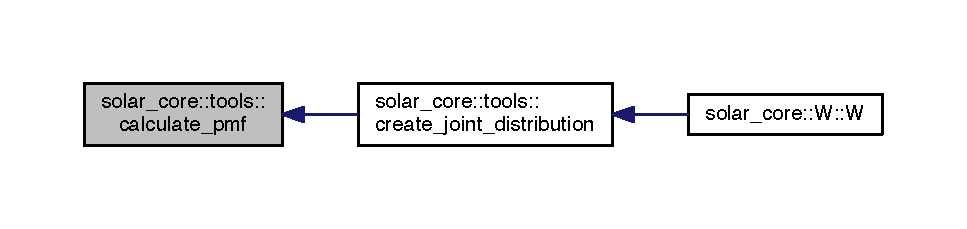
\includegraphics[width=350pt]{namespacesolar__core_1_1tools_a0afae1319ed9c683eba7bf2916d0850d_icgraph}
\end{center}
\end{figure}


\hypertarget{namespacesolar__core_1_1tools_a3994daf7d839df36bc1f424c426cb6a5}{}\index{solar\+\_\+core\+::tools@{solar\+\_\+core\+::tools}!calculate\+\_\+scale\+\_\+factor@{calculate\+\_\+scale\+\_\+factor}}
\index{calculate\+\_\+scale\+\_\+factor@{calculate\+\_\+scale\+\_\+factor}!solar\+\_\+core\+::tools@{solar\+\_\+core\+::tools}}
\subsubsection[{calculate\+\_\+scale\+\_\+factor}]{\setlength{\rightskip}{0pt plus 5cm}double solar\+\_\+core\+::tools\+::calculate\+\_\+scale\+\_\+factor (
\begin{DoxyParamCaption}
\item[{std\+::vector$<$ long $>$ \&}]{cond\+\_\+dist, }
\item[{{\bf Empirical\+U\+V\+D} \&}]{dist}
\end{DoxyParamCaption}
)}\label{namespacesolar__core_1_1tools_a3994daf7d839df36bc1f424c426cb6a5}


Definition at line 277 of file Simulation.\+cpp.



Here is the caller graph for this function\+:
\nopagebreak
\begin{figure}[H]
\begin{center}
\leavevmode
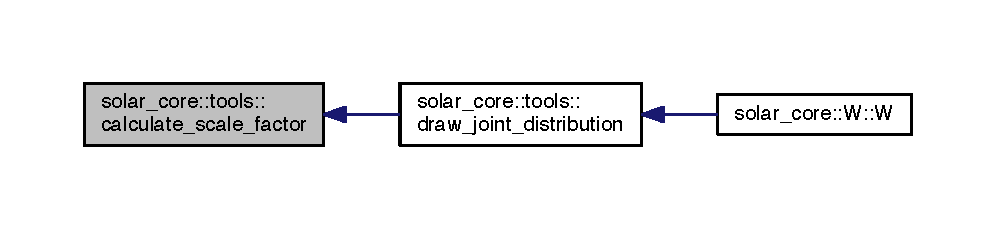
\includegraphics[width=350pt]{namespacesolar__core_1_1tools_a3994daf7d839df36bc1f424c426cb6a5_icgraph}
\end{center}
\end{figure}


\hypertarget{namespacesolar__core_1_1tools_ace8f7b4ee917995274fe32b95e27f6ef}{}\index{solar\+\_\+core\+::tools@{solar\+\_\+core\+::tools}!collapse\+\_\+pmf@{collapse\+\_\+pmf}}
\index{collapse\+\_\+pmf@{collapse\+\_\+pmf}!solar\+\_\+core\+::tools@{solar\+\_\+core\+::tools}}
\subsubsection[{collapse\+\_\+pmf}]{\setlength{\rightskip}{0pt plus 5cm}std\+::vector$<$ long $>$ solar\+\_\+core\+::tools\+::collapse\+\_\+pmf (
\begin{DoxyParamCaption}
\item[{std\+::vector$<$ long $>$ \&}]{i\+\_\+x, }
\item[{{\bf Empirical\+U\+V\+D} \&}]{dist}
\end{DoxyParamCaption}
)}\label{namespacesolar__core_1_1tools_ace8f7b4ee917995274fe32b95e27f6ef}


Definition at line 246 of file Simulation.\+cpp.



Here is the caller graph for this function\+:
\nopagebreak
\begin{figure}[H]
\begin{center}
\leavevmode
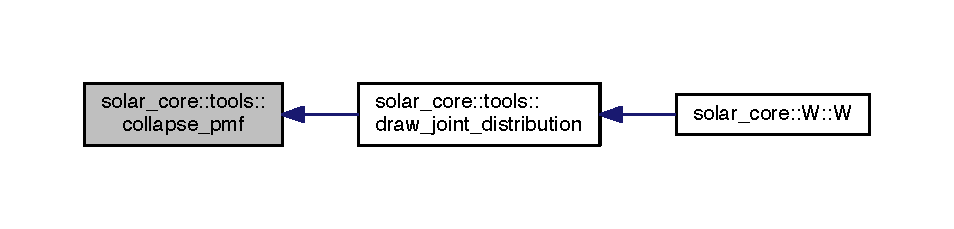
\includegraphics[width=350pt]{namespacesolar__core_1_1tools_ace8f7b4ee917995274fe32b95e27f6ef_icgraph}
\end{center}
\end{figure}


\hypertarget{namespacesolar__core_1_1tools_a09224182e02de7fdadabfba4e08e0ac2}{}\index{solar\+\_\+core\+::tools@{solar\+\_\+core\+::tools}!create\+\_\+cmf@{create\+\_\+cmf}}
\index{create\+\_\+cmf@{create\+\_\+cmf}!solar\+\_\+core\+::tools@{solar\+\_\+core\+::tools}}
\subsubsection[{create\+\_\+cmf}]{\setlength{\rightskip}{0pt plus 5cm}std\+::vector$<$ double $>$ solar\+\_\+core\+::tools\+::create\+\_\+cmf (
\begin{DoxyParamCaption}
\item[{std\+::vector$<$ long $>$ \&}]{cond\+\_\+dist, }
\item[{double}]{scale\+\_\+factor, }
\item[{{\bf Empirical\+U\+V\+D} \&}]{dist}
\end{DoxyParamCaption}
)}\label{namespacesolar__core_1_1tools_a09224182e02de7fdadabfba4e08e0ac2}


Definition at line 293 of file Simulation.\+cpp.



Here is the caller graph for this function\+:
\nopagebreak
\begin{figure}[H]
\begin{center}
\leavevmode
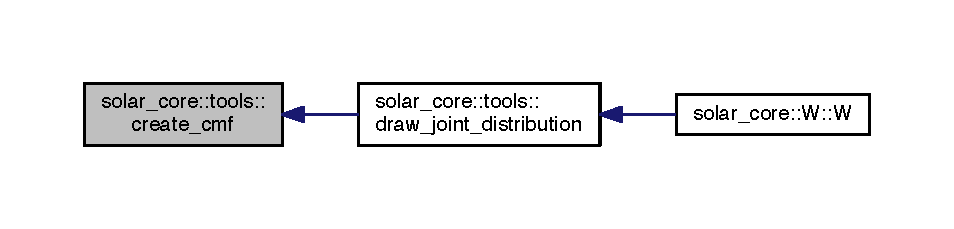
\includegraphics[width=350pt]{namespacesolar__core_1_1tools_a09224182e02de7fdadabfba4e08e0ac2_icgraph}
\end{center}
\end{figure}


\hypertarget{namespacesolar__core_1_1tools_a460021055d6057f219037f378c0c3248}{}\index{solar\+\_\+core\+::tools@{solar\+\_\+core\+::tools}!create\+\_\+joint\+\_\+distribution@{create\+\_\+joint\+\_\+distribution}}
\index{create\+\_\+joint\+\_\+distribution@{create\+\_\+joint\+\_\+distribution}!solar\+\_\+core\+::tools@{solar\+\_\+core\+::tools}}
\subsubsection[{create\+\_\+joint\+\_\+distribution}]{\setlength{\rightskip}{0pt plus 5cm}{\bf tools\+::\+Empirical\+M\+V\+D} solar\+\_\+core\+::tools\+::create\+\_\+joint\+\_\+distribution (
\begin{DoxyParamCaption}
\item[{std\+::string}]{path\+\_\+to\+\_\+scheme, }
\item[{std\+::string}]{path\+\_\+to\+\_\+data}
\end{DoxyParamCaption}
)}\label{namespacesolar__core_1_1tools_a460021055d6057f219037f378c0c3248}


Definition at line 17 of file Simulation.\+cpp.



Here is the call graph for this function\+:
\nopagebreak
\begin{figure}[H]
\begin{center}
\leavevmode
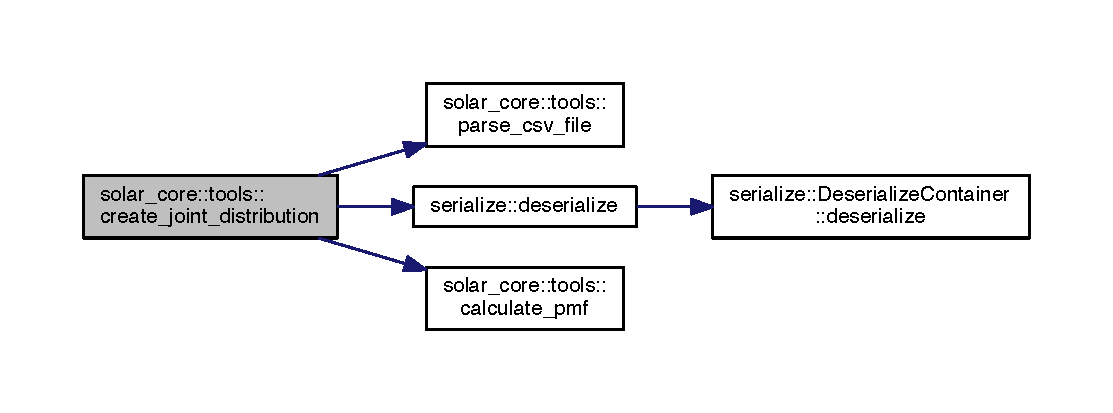
\includegraphics[width=350pt]{namespacesolar__core_1_1tools_a460021055d6057f219037f378c0c3248_cgraph}
\end{center}
\end{figure}




Here is the caller graph for this function\+:
\nopagebreak
\begin{figure}[H]
\begin{center}
\leavevmode
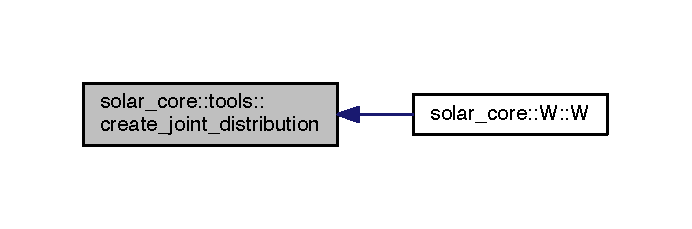
\includegraphics[width=332pt]{namespacesolar__core_1_1tools_a460021055d6057f219037f378c0c3248_icgraph}
\end{center}
\end{figure}


\hypertarget{namespacesolar__core_1_1tools_a1f6003e555b2d4261cc9f26ae2688427}{}\index{solar\+\_\+core\+::tools@{solar\+\_\+core\+::tools}!draw\+\_\+joint\+\_\+distribution@{draw\+\_\+joint\+\_\+distribution}}
\index{draw\+\_\+joint\+\_\+distribution@{draw\+\_\+joint\+\_\+distribution}!solar\+\_\+core\+::tools@{solar\+\_\+core\+::tools}}
\subsubsection[{draw\+\_\+joint\+\_\+distribution}]{\setlength{\rightskip}{0pt plus 5cm}std\+::vector$<$ double $>$ solar\+\_\+core\+::tools\+::draw\+\_\+joint\+\_\+distribution (
\begin{DoxyParamCaption}
\item[{{\bf Empirical\+M\+V\+D} \&}]{pmf, }
\item[{{\bf I\+Random} $\ast$}]{rand}
\end{DoxyParamCaption}
)}\label{namespacesolar__core_1_1tools_a1f6003e555b2d4261cc9f26ae2688427}


Definition at line 189 of file Simulation.\+cpp.



Here is the call graph for this function\+:
\nopagebreak
\begin{figure}[H]
\begin{center}
\leavevmode
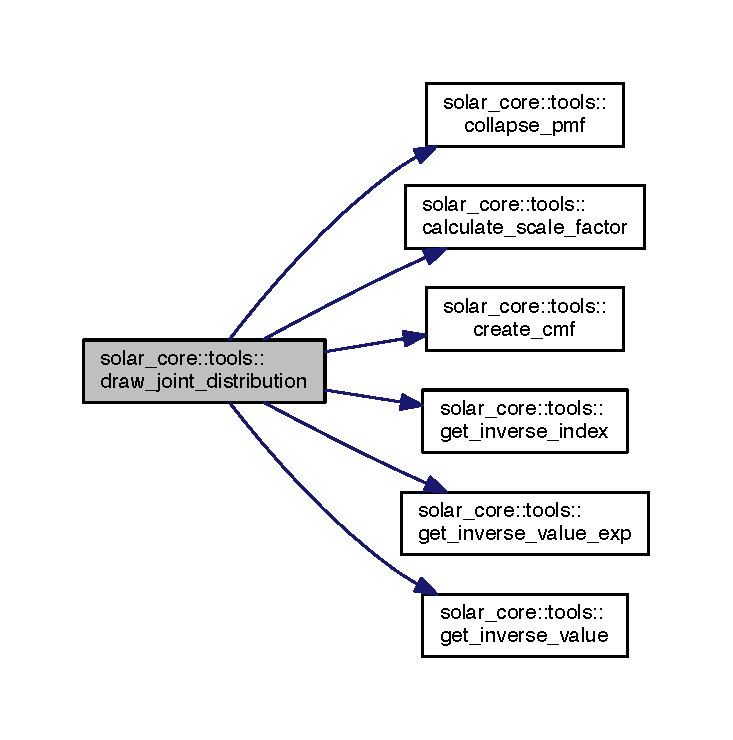
\includegraphics[width=350pt]{namespacesolar__core_1_1tools_a1f6003e555b2d4261cc9f26ae2688427_cgraph}
\end{center}
\end{figure}




Here is the caller graph for this function\+:
\nopagebreak
\begin{figure}[H]
\begin{center}
\leavevmode
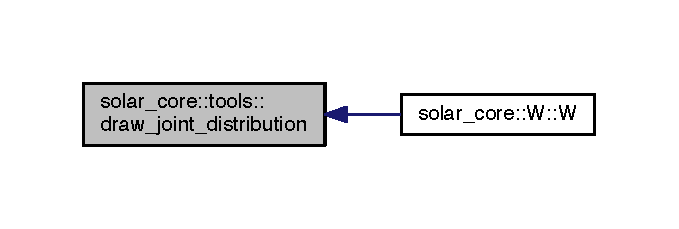
\includegraphics[width=326pt]{namespacesolar__core_1_1tools_a1f6003e555b2d4261cc9f26ae2688427_icgraph}
\end{center}
\end{figure}


\hypertarget{namespacesolar__core_1_1tools_a5826bf3d73d587e67bba31912e73862a}{}\index{solar\+\_\+core\+::tools@{solar\+\_\+core\+::tools}!get\+\_\+inverse\+\_\+index@{get\+\_\+inverse\+\_\+index}}
\index{get\+\_\+inverse\+\_\+index@{get\+\_\+inverse\+\_\+index}!solar\+\_\+core\+::tools@{solar\+\_\+core\+::tools}}
\subsubsection[{get\+\_\+inverse\+\_\+index}]{\setlength{\rightskip}{0pt plus 5cm}long solar\+\_\+core\+::tools\+::get\+\_\+inverse\+\_\+index (
\begin{DoxyParamCaption}
\item[{std\+::vector$<$ double $>$ \&}]{cmf, }
\item[{double}]{u\+\_\+i}
\end{DoxyParamCaption}
)}\label{namespacesolar__core_1_1tools_a5826bf3d73d587e67bba31912e73862a}


Definition at line 327 of file Simulation.\+cpp.



Here is the caller graph for this function\+:
\nopagebreak
\begin{figure}[H]
\begin{center}
\leavevmode
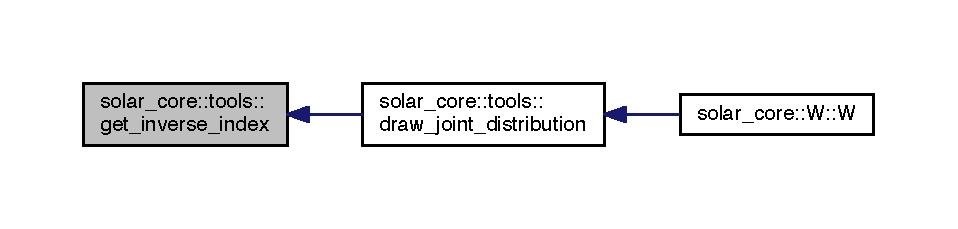
\includegraphics[width=350pt]{namespacesolar__core_1_1tools_a5826bf3d73d587e67bba31912e73862a_icgraph}
\end{center}
\end{figure}


\hypertarget{namespacesolar__core_1_1tools_a97e71ce44bf9e2eedbcce4332e8fcdd8}{}\index{solar\+\_\+core\+::tools@{solar\+\_\+core\+::tools}!get\+\_\+inverse\+\_\+value@{get\+\_\+inverse\+\_\+value}}
\index{get\+\_\+inverse\+\_\+value@{get\+\_\+inverse\+\_\+value}!solar\+\_\+core\+::tools@{solar\+\_\+core\+::tools}}
\subsubsection[{get\+\_\+inverse\+\_\+value}]{\setlength{\rightskip}{0pt plus 5cm}double solar\+\_\+core\+::tools\+::get\+\_\+inverse\+\_\+value (
\begin{DoxyParamCaption}
\item[{std\+::vector$<$ double $>$ \&}]{theta\+\_\+bin, }
\item[{double}]{u\+\_\+i}
\end{DoxyParamCaption}
)}\label{namespacesolar__core_1_1tools_a97e71ce44bf9e2eedbcce4332e8fcdd8}


Definition at line 345 of file Simulation.\+cpp.



Here is the caller graph for this function\+:
\nopagebreak
\begin{figure}[H]
\begin{center}
\leavevmode
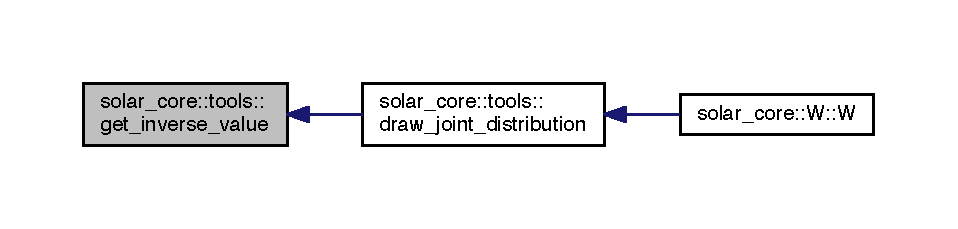
\includegraphics[width=350pt]{namespacesolar__core_1_1tools_a97e71ce44bf9e2eedbcce4332e8fcdd8_icgraph}
\end{center}
\end{figure}


\hypertarget{namespacesolar__core_1_1tools_ab3631c4cd4d3cc65b4b8d59171809060}{}\index{solar\+\_\+core\+::tools@{solar\+\_\+core\+::tools}!get\+\_\+inverse\+\_\+value\+\_\+exp@{get\+\_\+inverse\+\_\+value\+\_\+exp}}
\index{get\+\_\+inverse\+\_\+value\+\_\+exp@{get\+\_\+inverse\+\_\+value\+\_\+exp}!solar\+\_\+core\+::tools@{solar\+\_\+core\+::tools}}
\subsubsection[{get\+\_\+inverse\+\_\+value\+\_\+exp}]{\setlength{\rightskip}{0pt plus 5cm}double solar\+\_\+core\+::tools\+::get\+\_\+inverse\+\_\+value\+\_\+exp (
\begin{DoxyParamCaption}
\item[{std\+::vector$<$ double $>$ \&}]{theta\+\_\+bin, }
\item[{double}]{u\+\_\+i}
\end{DoxyParamCaption}
)}\label{namespacesolar__core_1_1tools_ab3631c4cd4d3cc65b4b8d59171809060}


Definition at line 353 of file Simulation.\+cpp.



Here is the caller graph for this function\+:
\nopagebreak
\begin{figure}[H]
\begin{center}
\leavevmode
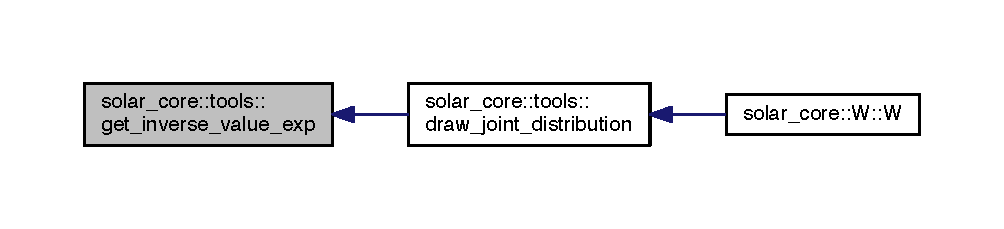
\includegraphics[width=350pt]{namespacesolar__core_1_1tools_ab3631c4cd4d3cc65b4b8d59171809060_icgraph}
\end{center}
\end{figure}


\hypertarget{namespacesolar__core_1_1tools_ae8bc4dd0c291632fc369b647480c30eb}{}\index{solar\+\_\+core\+::tools@{solar\+\_\+core\+::tools}!parse\+\_\+csv\+\_\+file@{parse\+\_\+csv\+\_\+file}}
\index{parse\+\_\+csv\+\_\+file@{parse\+\_\+csv\+\_\+file}!solar\+\_\+core\+::tools@{solar\+\_\+core\+::tools}}
\subsubsection[{parse\+\_\+csv\+\_\+file}]{\setlength{\rightskip}{0pt plus 5cm}template$<$class T $>$ void solar\+\_\+core\+::tools\+::parse\+\_\+csv\+\_\+file (
\begin{DoxyParamCaption}
\item[{std\+::string}]{path\+\_\+to\+\_\+file, }
\item[{std\+::vector$<$ std\+::vector$<$ T $>$$>$ \&}]{parsed\+\_\+file}
\end{DoxyParamCaption}
)}\label{namespacesolar__core_1_1tools_ae8bc4dd0c291632fc369b647480c30eb}


Definition at line 23 of file Parsing\+Tools.\+h.



Here is the caller graph for this function\+:
\nopagebreak
\begin{figure}[H]
\begin{center}
\leavevmode
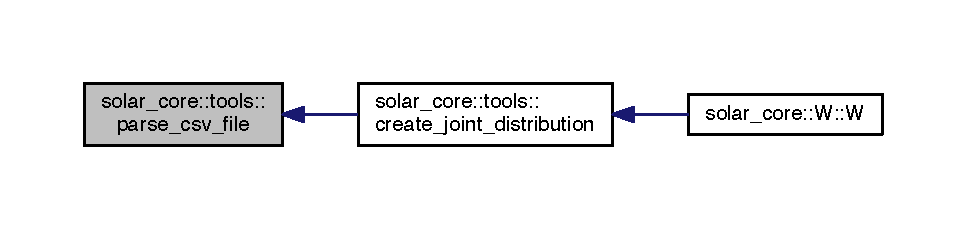
\includegraphics[width=350pt]{namespacesolar__core_1_1tools_ae8bc4dd0c291632fc369b647480c30eb_icgraph}
\end{center}
\end{figure}


\hypertarget{namespacesolar__core_1_1tools_ad27b346e42787b5220c80cd386eae266}{}\index{solar\+\_\+core\+::tools@{solar\+\_\+core\+::tools}!parse\+\_\+model\+\_\+file@{parse\+\_\+model\+\_\+file}}
\index{parse\+\_\+model\+\_\+file@{parse\+\_\+model\+\_\+file}!solar\+\_\+core\+::tools@{solar\+\_\+core\+::tools}}
\subsubsection[{parse\+\_\+model\+\_\+file}]{\setlength{\rightskip}{0pt plus 5cm}void solar\+\_\+core\+::tools\+::parse\+\_\+model\+\_\+file (
\begin{DoxyParamCaption}
\item[{std\+::string}]{path\+\_\+to\+\_\+file, }
\item[{std\+::map$<$ std\+::string, std\+::string $>$ \&}]{parsed\+\_\+model}
\end{DoxyParamCaption}
)}\label{namespacesolar__core_1_1tools_ad27b346e42787b5220c80cd386eae266}


Definition at line 18 of file Parsing\+Tools.\+cpp.



Here is the caller graph for this function\+:\nopagebreak
\begin{figure}[H]
\begin{center}
\leavevmode
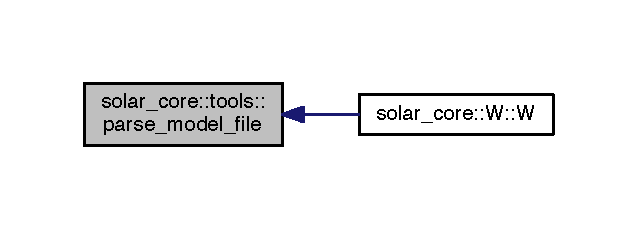
\includegraphics[width=306pt]{namespacesolar__core_1_1tools_ad27b346e42787b5220c80cd386eae266_icgraph}
\end{center}
\end{figure}



\hypertarget{namespacesolar__ui}{}\section{solar\+\_\+ui Namespace Reference}
\label{namespacesolar__ui}\index{solar\+\_\+ui@{solar\+\_\+ui}}
\subsection*{Classes}
\begin{DoxyCompactItemize}
\item 
class \hyperlink{classsolar__ui_1_1_u_i}{U\+I}
\end{DoxyCompactItemize}

\chapter{Class Documentation}
\hypertarget{classsolar__core_1_1_baseline_model}{}\section{solar\+\_\+core\+:\+:Baseline\+Model Class Reference}
\label{classsolar__core_1_1_baseline_model}\index{solar\+\_\+core\+::\+Baseline\+Model@{solar\+\_\+core\+::\+Baseline\+Model}}


{\ttfamily \#include $<$Helper\+W.\+h$>$}



\subsection{Detailed Description}


Definition at line 25 of file Helper\+W.\+h.



The documentation for this class was generated from the following file\+:\begin{DoxyCompactItemize}
\item 
/\+Users/wilfeli/\+Dropbox/\+A\+B\+M/\+Solar\+Panels/\+A\+B\+M\+I\+R\+I\+S\+Lab/\+Source/\+U\+I/\hyperlink{_helper_w_8h}{Helper\+W.\+h}\end{DoxyCompactItemize}

\hypertarget{classserialize_1_1_deserialize_container}{}\section{serialize\+:\+:Deserialize\+Container$<$ T, Enable $>$ Class Template Reference}
\label{classserialize_1_1_deserialize_container}\index{serialize\+::\+Deserialize\+Container$<$ T, Enable $>$@{serialize\+::\+Deserialize\+Container$<$ T, Enable $>$}}


{\ttfamily \#include $<$Serialize.\+h$>$}

\subsection*{Static Public Member Functions}
\begin{DoxyCompactItemize}
\item 
static void \hyperlink{classserialize_1_1_deserialize_container_a81bdeaff0ef56f203cc65b1d0691c471}{deserialize} (const \hyperlink{namespacesolar__core_adeda2737d6938c190eb774a5b2495045}{Property\+Tree} \&pt, std\+::vector$<$ T $>$ \&r)
\item 
static void \hyperlink{classserialize_1_1_deserialize_container_a393ffc783bcb56715d088fd615d9fe3e}{deserialize} (const \hyperlink{namespacesolar__core_adeda2737d6938c190eb774a5b2495045}{Property\+Tree} \&pt, std\+::deque$<$ T $>$ \&r)
\end{DoxyCompactItemize}


\subsection{Detailed Description}
\subsubsection*{template$<$class T, class Enable = void$>$class serialize\+::\+Deserialize\+Container$<$ T, Enable $>$}



Definition at line 242 of file Serialize.\+h.



\subsection{Member Function Documentation}
\hypertarget{classserialize_1_1_deserialize_container_a81bdeaff0ef56f203cc65b1d0691c471}{}\index{serialize\+::\+Deserialize\+Container@{serialize\+::\+Deserialize\+Container}!deserialize@{deserialize}}
\index{deserialize@{deserialize}!serialize\+::\+Deserialize\+Container@{serialize\+::\+Deserialize\+Container}}
\subsubsection[{deserialize}]{\setlength{\rightskip}{0pt plus 5cm}template$<$class T , class Enable  = void$>$ static void {\bf serialize\+::\+Deserialize\+Container}$<$ T, Enable $>$\+::deserialize (
\begin{DoxyParamCaption}
\item[{const {\bf Property\+Tree} \&}]{pt, }
\item[{std\+::vector$<$ T $>$ \&}]{r}
\end{DoxyParamCaption}
)\hspace{0.3cm}{\ttfamily [inline]}, {\ttfamily [static]}}\label{classserialize_1_1_deserialize_container_a81bdeaff0ef56f203cc65b1d0691c471}


Definition at line 246 of file Serialize.\+h.



Here is the caller graph for this function\+:
\nopagebreak
\begin{figure}[H]
\begin{center}
\leavevmode
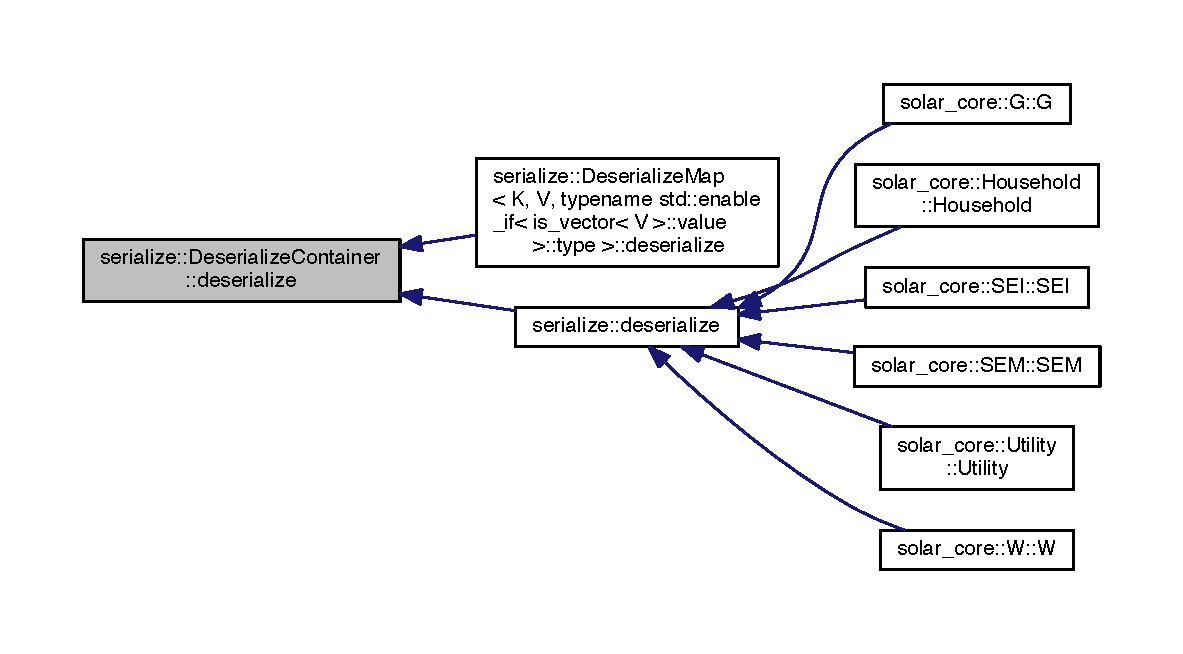
\includegraphics[width=350pt]{classserialize_1_1_deserialize_container_a81bdeaff0ef56f203cc65b1d0691c471_icgraph}
\end{center}
\end{figure}


\hypertarget{classserialize_1_1_deserialize_container_a393ffc783bcb56715d088fd615d9fe3e}{}\index{serialize\+::\+Deserialize\+Container@{serialize\+::\+Deserialize\+Container}!deserialize@{deserialize}}
\index{deserialize@{deserialize}!serialize\+::\+Deserialize\+Container@{serialize\+::\+Deserialize\+Container}}
\subsubsection[{deserialize}]{\setlength{\rightskip}{0pt plus 5cm}template$<$class T , class Enable  = void$>$ static void {\bf serialize\+::\+Deserialize\+Container}$<$ T, Enable $>$\+::deserialize (
\begin{DoxyParamCaption}
\item[{const {\bf Property\+Tree} \&}]{pt, }
\item[{std\+::deque$<$ T $>$ \&}]{r}
\end{DoxyParamCaption}
)\hspace{0.3cm}{\ttfamily [inline]}, {\ttfamily [static]}}\label{classserialize_1_1_deserialize_container_a393ffc783bcb56715d088fd615d9fe3e}


Definition at line 254 of file Serialize.\+h.



The documentation for this class was generated from the following file\+:\begin{DoxyCompactItemize}
\item 
/\+Users/wilfeli/\+Dropbox/\+A\+B\+M/\+Solar\+Panels/\+A\+B\+M\+I\+R\+I\+S\+Lab/\+Source/\+Tools/\hyperlink{_serialize_8h}{Serialize.\+h}\end{DoxyCompactItemize}

\hypertarget{classserialize_1_1_deserialize_map}{}\section{serialize\+:\+:Deserialize\+Map$<$ K, V, Enable $>$ Class Template Reference}
\label{classserialize_1_1_deserialize_map}\index{serialize\+::\+Deserialize\+Map$<$ K, V, Enable $>$@{serialize\+::\+Deserialize\+Map$<$ K, V, Enable $>$}}


{\ttfamily \#include $<$Serialize.\+h$>$}

\subsection*{Static Public Member Functions}
\begin{DoxyCompactItemize}
\item 
static void \hyperlink{classserialize_1_1_deserialize_map_af4827270beb08c018e840b9cec766cde}{deserialize} (const \hyperlink{namespacesolar__core_adeda2737d6938c190eb774a5b2495045}{Property\+Tree} \&pt, std\+::map$<$ K, V $>$ \&r)
\end{DoxyCompactItemize}


\subsection{Detailed Description}
\subsubsection*{template$<$class K, class V, class Enable = void$>$class serialize\+::\+Deserialize\+Map$<$ K, V, Enable $>$}

General template for serializatio of a map 

Definition at line 280 of file Serialize.\+h.



\subsection{Member Function Documentation}
\hypertarget{classserialize_1_1_deserialize_map_af4827270beb08c018e840b9cec766cde}{}\index{serialize\+::\+Deserialize\+Map@{serialize\+::\+Deserialize\+Map}!deserialize@{deserialize}}
\index{deserialize@{deserialize}!serialize\+::\+Deserialize\+Map@{serialize\+::\+Deserialize\+Map}}
\subsubsection[{deserialize}]{\setlength{\rightskip}{0pt plus 5cm}template$<$class K , class V , class Enable  = void$>$ static void {\bf serialize\+::\+Deserialize\+Map}$<$ K, V, Enable $>$\+::deserialize (
\begin{DoxyParamCaption}
\item[{const {\bf Property\+Tree} \&}]{pt, }
\item[{std\+::map$<$ K, V $>$ \&}]{r}
\end{DoxyParamCaption}
)\hspace{0.3cm}{\ttfamily [inline]}, {\ttfamily [static]}}\label{classserialize_1_1_deserialize_map_af4827270beb08c018e840b9cec766cde}


Definition at line 283 of file Serialize.\+h.



Here is the call graph for this function\+:\nopagebreak
\begin{figure}[H]
\begin{center}
\leavevmode
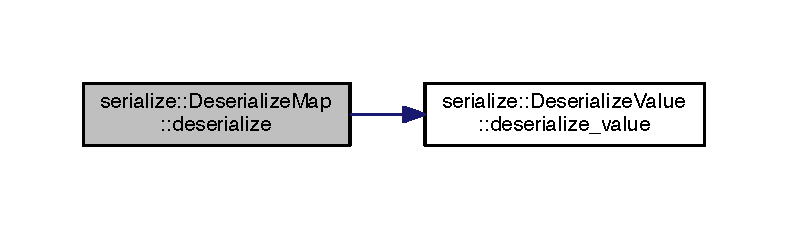
\includegraphics[width=350pt]{classserialize_1_1_deserialize_map_af4827270beb08c018e840b9cec766cde_cgraph}
\end{center}
\end{figure}




Here is the caller graph for this function\+:
\nopagebreak
\begin{figure}[H]
\begin{center}
\leavevmode
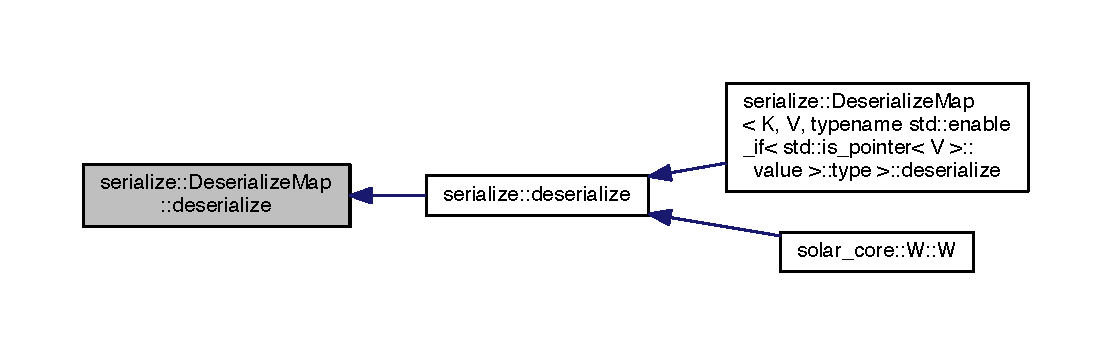
\includegraphics[width=350pt]{classserialize_1_1_deserialize_map_af4827270beb08c018e840b9cec766cde_icgraph}
\end{center}
\end{figure}




The documentation for this class was generated from the following file\+:\begin{DoxyCompactItemize}
\item 
/\+Users/wilfeli/\+Dropbox/\+A\+B\+M/\+Solar\+Panels/\+A\+B\+M\+I\+R\+I\+S\+Lab/\+Source/\+Tools/\hyperlink{_serialize_8h}{Serialize.\+h}\end{DoxyCompactItemize}

\hypertarget{classserialize_1_1_deserialize_map_3_01_k_00_01std_1_1shared__ptr_3_01_v_01_4_01_4}{}\section{serialize\+:\+:Deserialize\+Map$<$ K, std\+:\+:shared\+\_\+ptr$<$ V $>$ $>$ Class Template Reference}
\label{classserialize_1_1_deserialize_map_3_01_k_00_01std_1_1shared__ptr_3_01_v_01_4_01_4}\index{serialize\+::\+Deserialize\+Map$<$ K, std\+::shared\+\_\+ptr$<$ V $>$ $>$@{serialize\+::\+Deserialize\+Map$<$ K, std\+::shared\+\_\+ptr$<$ V $>$ $>$}}


{\ttfamily \#include $<$Serialize.\+h$>$}

\subsection*{Static Public Member Functions}
\begin{DoxyCompactItemize}
\item 
static void \hyperlink{classserialize_1_1_deserialize_map_3_01_k_00_01std_1_1shared__ptr_3_01_v_01_4_01_4_ad2807cf1ee4670cbda806ad46c57f360}{deserialize} (const \hyperlink{namespacesolar__core_adeda2737d6938c190eb774a5b2495045}{Property\+Tree} \&pt, std\+::map$<$ K, std\+::shared\+\_\+ptr$<$ V $>$$>$ \&r)
\end{DoxyCompactItemize}


\subsection{Detailed Description}
\subsubsection*{template$<$class K, class V$>$class serialize\+::\+Deserialize\+Map$<$ K, std\+::shared\+\_\+ptr$<$ V $>$ $>$}



Definition at line 337 of file Serialize.\+h.



\subsection{Member Function Documentation}
\hypertarget{classserialize_1_1_deserialize_map_3_01_k_00_01std_1_1shared__ptr_3_01_v_01_4_01_4_ad2807cf1ee4670cbda806ad46c57f360}{}\index{serialize\+::\+Deserialize\+Map$<$ K, std\+::shared\+\_\+ptr$<$ V $>$ $>$@{serialize\+::\+Deserialize\+Map$<$ K, std\+::shared\+\_\+ptr$<$ V $>$ $>$}!deserialize@{deserialize}}
\index{deserialize@{deserialize}!serialize\+::\+Deserialize\+Map$<$ K, std\+::shared\+\_\+ptr$<$ V $>$ $>$@{serialize\+::\+Deserialize\+Map$<$ K, std\+::shared\+\_\+ptr$<$ V $>$ $>$}}
\subsubsection[{deserialize}]{\setlength{\rightskip}{0pt plus 5cm}template$<$class K , class V $>$ static void {\bf serialize\+::\+Deserialize\+Map}$<$ K, std\+::shared\+\_\+ptr$<$ V $>$ $>$\+::deserialize (
\begin{DoxyParamCaption}
\item[{const {\bf Property\+Tree} \&}]{pt, }
\item[{std\+::map$<$ K, std\+::shared\+\_\+ptr$<$ V $>$$>$ \&}]{r}
\end{DoxyParamCaption}
)\hspace{0.3cm}{\ttfamily [inline]}, {\ttfamily [static]}}\label{classserialize_1_1_deserialize_map_3_01_k_00_01std_1_1shared__ptr_3_01_v_01_4_01_4_ad2807cf1ee4670cbda806ad46c57f360}


Definition at line 340 of file Serialize.\+h.



Here is the call graph for this function\+:\nopagebreak
\begin{figure}[H]
\begin{center}
\leavevmode
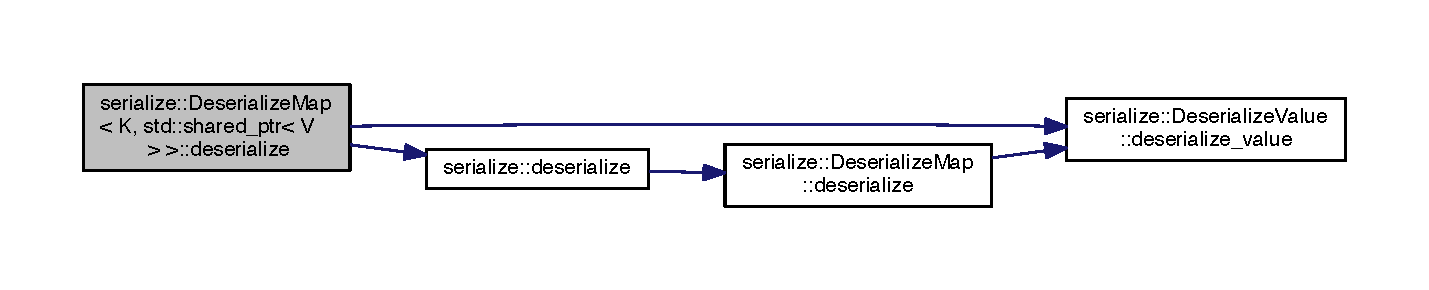
\includegraphics[width=350pt]{classserialize_1_1_deserialize_map_3_01_k_00_01std_1_1shared__ptr_3_01_v_01_4_01_4_ad2807cf1ee4670cbda806ad46c57f360_cgraph}
\end{center}
\end{figure}




The documentation for this class was generated from the following file\+:\begin{DoxyCompactItemize}
\item 
/\+Users/wilfeli/\+Dropbox/\+A\+B\+M/\+Solar\+Panels/\+A\+B\+M\+I\+R\+I\+S\+Lab/\+Source/\+Tools/\hyperlink{_serialize_8h}{Serialize.\+h}\end{DoxyCompactItemize}

\hypertarget{classserialize_1_1_deserialize_map_3_01_k_00_01_v_00_01typename_01std_1_1enable__if_3_01is__vected2d1ee1f8886a5a92a6dbc69e18bdcd}{}\section{serialize\+:\+:Deserialize\+Map$<$ K, V, typename std\+:\+:enable\+\_\+if$<$ is\+\_\+vector$<$ V $>$\+:\+:value $>$\+:\+:type $>$ Class Template Reference}
\label{classserialize_1_1_deserialize_map_3_01_k_00_01_v_00_01typename_01std_1_1enable__if_3_01is__vected2d1ee1f8886a5a92a6dbc69e18bdcd}\index{serialize\+::\+Deserialize\+Map$<$ K, V, typename std\+::enable\+\_\+if$<$ is\+\_\+vector$<$ V $>$\+::value $>$\+::type $>$@{serialize\+::\+Deserialize\+Map$<$ K, V, typename std\+::enable\+\_\+if$<$ is\+\_\+vector$<$ V $>$\+::value $>$\+::type $>$}}


{\ttfamily \#include $<$Serialize.\+h$>$}

\subsection*{Static Public Member Functions}
\begin{DoxyCompactItemize}
\item 
static void \hyperlink{classserialize_1_1_deserialize_map_3_01_k_00_01_v_00_01typename_01std_1_1enable__if_3_01is__vected2d1ee1f8886a5a92a6dbc69e18bdcd_a4ac8a4888f9383e338904ed4ea0ab4a7}{deserialize} (const \hyperlink{namespacesolar__core_adeda2737d6938c190eb774a5b2495045}{Property\+Tree} \&pt, std\+::map$<$ K, V $>$ \&r)
\end{DoxyCompactItemize}


\subsection{Detailed Description}
\subsubsection*{template$<$class K, class V$>$class serialize\+::\+Deserialize\+Map$<$ K, V, typename std\+::enable\+\_\+if$<$ is\+\_\+vector$<$ V $>$\+::value $>$\+::type $>$}



Definition at line 358 of file Serialize.\+h.



\subsection{Member Function Documentation}
\hypertarget{classserialize_1_1_deserialize_map_3_01_k_00_01_v_00_01typename_01std_1_1enable__if_3_01is__vected2d1ee1f8886a5a92a6dbc69e18bdcd_a4ac8a4888f9383e338904ed4ea0ab4a7}{}\index{serialize\+::\+Deserialize\+Map$<$ K, V, typename std\+::enable\+\_\+if$<$ is\+\_\+vector$<$ V $>$\+::value $>$\+::type $>$@{serialize\+::\+Deserialize\+Map$<$ K, V, typename std\+::enable\+\_\+if$<$ is\+\_\+vector$<$ V $>$\+::value $>$\+::type $>$}!deserialize@{deserialize}}
\index{deserialize@{deserialize}!serialize\+::\+Deserialize\+Map$<$ K, V, typename std\+::enable\+\_\+if$<$ is\+\_\+vector$<$ V $>$\+::value $>$\+::type $>$@{serialize\+::\+Deserialize\+Map$<$ K, V, typename std\+::enable\+\_\+if$<$ is\+\_\+vector$<$ V $>$\+::value $>$\+::type $>$}}
\subsubsection[{deserialize}]{\setlength{\rightskip}{0pt plus 5cm}template$<$class K , class V $>$ static void {\bf serialize\+::\+Deserialize\+Map}$<$ K, V, typename std\+::enable\+\_\+if$<$ {\bf is\+\_\+vector}$<$ V $>$\+::value $>$\+::type $>$\+::deserialize (
\begin{DoxyParamCaption}
\item[{const {\bf Property\+Tree} \&}]{pt, }
\item[{std\+::map$<$ K, V $>$ \&}]{r}
\end{DoxyParamCaption}
)\hspace{0.3cm}{\ttfamily [inline]}, {\ttfamily [static]}}\label{classserialize_1_1_deserialize_map_3_01_k_00_01_v_00_01typename_01std_1_1enable__if_3_01is__vected2d1ee1f8886a5a92a6dbc69e18bdcd_a4ac8a4888f9383e338904ed4ea0ab4a7}


Definition at line 361 of file Serialize.\+h.



Here is the call graph for this function\+:
\nopagebreak
\begin{figure}[H]
\begin{center}
\leavevmode
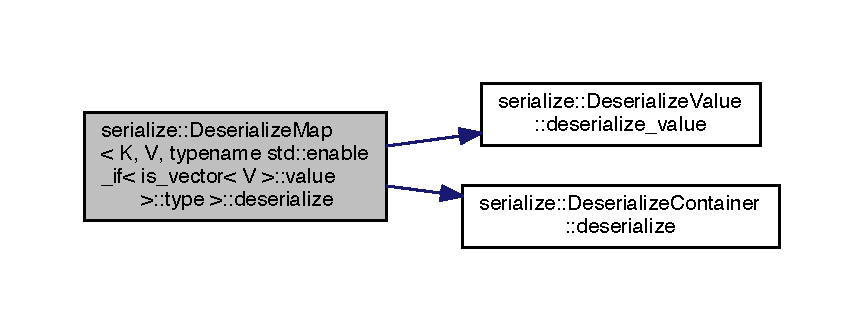
\includegraphics[width=350pt]{classserialize_1_1_deserialize_map_3_01_k_00_01_v_00_01typename_01std_1_1enable__if_3_01is__vected2d1ee1f8886a5a92a6dbc69e18bdcd_a4ac8a4888f9383e338904ed4ea0ab4a7_cgraph}
\end{center}
\end{figure}




The documentation for this class was generated from the following file\+:\begin{DoxyCompactItemize}
\item 
/\+Users/wilfeli/\+Dropbox/\+A\+B\+M/\+Solar\+Panels/\+A\+B\+M\+I\+R\+I\+S\+Lab/\+Source/\+Tools/\hyperlink{_serialize_8h}{Serialize.\+h}\end{DoxyCompactItemize}

\hypertarget{classserialize_1_1_deserialize_map_3_01_k_00_01_v_00_01typename_01std_1_1enable__if_3_01std_1_1ibe6cfa8a2d341f3a0942baedd95196d5}{}\section{serialize\+:\+:Deserialize\+Map$<$ K, V, typename std\+:\+:enable\+\_\+if$<$ std\+:\+:is\+\_\+pointer$<$ V $>$\+:\+:value $>$\+:\+:type $>$ Class Template Reference}
\label{classserialize_1_1_deserialize_map_3_01_k_00_01_v_00_01typename_01std_1_1enable__if_3_01std_1_1ibe6cfa8a2d341f3a0942baedd95196d5}\index{serialize\+::\+Deserialize\+Map$<$ K, V, typename std\+::enable\+\_\+if$<$ std\+::is\+\_\+pointer$<$ V $>$\+::value $>$\+::type $>$@{serialize\+::\+Deserialize\+Map$<$ K, V, typename std\+::enable\+\_\+if$<$ std\+::is\+\_\+pointer$<$ V $>$\+::value $>$\+::type $>$}}


{\ttfamily \#include $<$Serialize.\+h$>$}

\subsection*{Static Public Member Functions}
\begin{DoxyCompactItemize}
\item 
static void \hyperlink{classserialize_1_1_deserialize_map_3_01_k_00_01_v_00_01typename_01std_1_1enable__if_3_01std_1_1ibe6cfa8a2d341f3a0942baedd95196d5_ad440b5c02ce0eb7839f46df2e95f93ee}{deserialize} (const \hyperlink{namespacesolar__core_adeda2737d6938c190eb774a5b2495045}{Property\+Tree} \&pt, std\+::map$<$ K, V $>$ \&r)
\end{DoxyCompactItemize}


\subsection{Detailed Description}
\subsubsection*{template$<$class K, class V$>$class serialize\+::\+Deserialize\+Map$<$ K, V, typename std\+::enable\+\_\+if$<$ std\+::is\+\_\+pointer$<$ V $>$\+::value $>$\+::type $>$}



Definition at line 300 of file Serialize.\+h.



\subsection{Member Function Documentation}
\hypertarget{classserialize_1_1_deserialize_map_3_01_k_00_01_v_00_01typename_01std_1_1enable__if_3_01std_1_1ibe6cfa8a2d341f3a0942baedd95196d5_ad440b5c02ce0eb7839f46df2e95f93ee}{}\index{serialize\+::\+Deserialize\+Map$<$ K, V, typename std\+::enable\+\_\+if$<$ std\+::is\+\_\+pointer$<$ V $>$\+::value $>$\+::type $>$@{serialize\+::\+Deserialize\+Map$<$ K, V, typename std\+::enable\+\_\+if$<$ std\+::is\+\_\+pointer$<$ V $>$\+::value $>$\+::type $>$}!deserialize@{deserialize}}
\index{deserialize@{deserialize}!serialize\+::\+Deserialize\+Map$<$ K, V, typename std\+::enable\+\_\+if$<$ std\+::is\+\_\+pointer$<$ V $>$\+::value $>$\+::type $>$@{serialize\+::\+Deserialize\+Map$<$ K, V, typename std\+::enable\+\_\+if$<$ std\+::is\+\_\+pointer$<$ V $>$\+::value $>$\+::type $>$}}
\subsubsection[{deserialize}]{\setlength{\rightskip}{0pt plus 5cm}template$<$class K , class V $>$ static void {\bf serialize\+::\+Deserialize\+Map}$<$ K, V, typename std\+::enable\+\_\+if$<$ std\+::is\+\_\+pointer$<$ V $>$\+::value $>$\+::type $>$\+::deserialize (
\begin{DoxyParamCaption}
\item[{const {\bf Property\+Tree} \&}]{pt, }
\item[{std\+::map$<$ K, V $>$ \&}]{r}
\end{DoxyParamCaption}
)\hspace{0.3cm}{\ttfamily [inline]}, {\ttfamily [static]}}\label{classserialize_1_1_deserialize_map_3_01_k_00_01_v_00_01typename_01std_1_1enable__if_3_01std_1_1ibe6cfa8a2d341f3a0942baedd95196d5_ad440b5c02ce0eb7839f46df2e95f93ee}


Definition at line 303 of file Serialize.\+h.



Here is the call graph for this function\+:\nopagebreak
\begin{figure}[H]
\begin{center}
\leavevmode
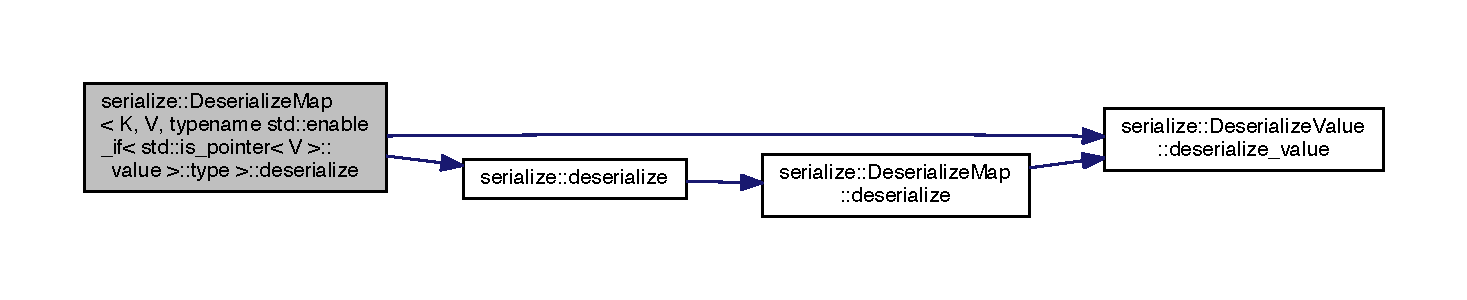
\includegraphics[width=350pt]{classserialize_1_1_deserialize_map_3_01_k_00_01_v_00_01typename_01std_1_1enable__if_3_01std_1_1ibe6cfa8a2d341f3a0942baedd95196d5_ad440b5c02ce0eb7839f46df2e95f93ee_cgraph}
\end{center}
\end{figure}




The documentation for this class was generated from the following file\+:\begin{DoxyCompactItemize}
\item 
/\+Users/wilfeli/\+Dropbox/\+A\+B\+M/\+Solar\+Panels/\+A\+B\+M\+I\+R\+I\+S\+Lab/\+Source/\+Tools/\hyperlink{_serialize_8h}{Serialize.\+h}\end{DoxyCompactItemize}

\hypertarget{classserialize_1_1_deserialize_value}{}\section{serialize\+:\+:Deserialize\+Value$<$ T, Enable $>$ Class Template Reference}
\label{classserialize_1_1_deserialize_value}\index{serialize\+::\+Deserialize\+Value$<$ T, Enable $>$@{serialize\+::\+Deserialize\+Value$<$ T, Enable $>$}}


{\ttfamily \#include $<$Serialize.\+h$>$}

\subsection*{Static Public Member Functions}
\begin{DoxyCompactItemize}
\item 
static void \hyperlink{classserialize_1_1_deserialize_value_ae086cfe3996b96c0a82785afe0af81b1}{deserialize\+\_\+value} (const std\+::string \&in\+\_\+, T \&out\+\_\+)
\item 
static void \hyperlink{classserialize_1_1_deserialize_value_a85960dc8ca3587ca9c275c0deb679bb7}{deserialize\+\_\+value} (std\+::stringstream \&ss, T \&out\+\_\+)
\end{DoxyCompactItemize}


\subsection{Detailed Description}
\subsubsection*{template$<$class T, class Enable = void$>$class serialize\+::\+Deserialize\+Value$<$ T, Enable $>$}



Definition at line 67 of file Serialize.\+h.



\subsection{Member Function Documentation}
\hypertarget{classserialize_1_1_deserialize_value_ae086cfe3996b96c0a82785afe0af81b1}{}\index{serialize\+::\+Deserialize\+Value@{serialize\+::\+Deserialize\+Value}!deserialize\+\_\+value@{deserialize\+\_\+value}}
\index{deserialize\+\_\+value@{deserialize\+\_\+value}!serialize\+::\+Deserialize\+Value@{serialize\+::\+Deserialize\+Value}}
\subsubsection[{deserialize\+\_\+value}]{\setlength{\rightskip}{0pt plus 5cm}template$<$class T , class Enable  = void$>$ static void {\bf serialize\+::\+Deserialize\+Value}$<$ T, Enable $>$\+::deserialize\+\_\+value (
\begin{DoxyParamCaption}
\item[{const std\+::string \&}]{in\+\_\+, }
\item[{T \&}]{out\+\_\+}
\end{DoxyParamCaption}
)\hspace{0.3cm}{\ttfamily [inline]}, {\ttfamily [static]}}\label{classserialize_1_1_deserialize_value_ae086cfe3996b96c0a82785afe0af81b1}


Definition at line 70 of file Serialize.\+h.



Here is the caller graph for this function\+:
\nopagebreak
\begin{figure}[H]
\begin{center}
\leavevmode
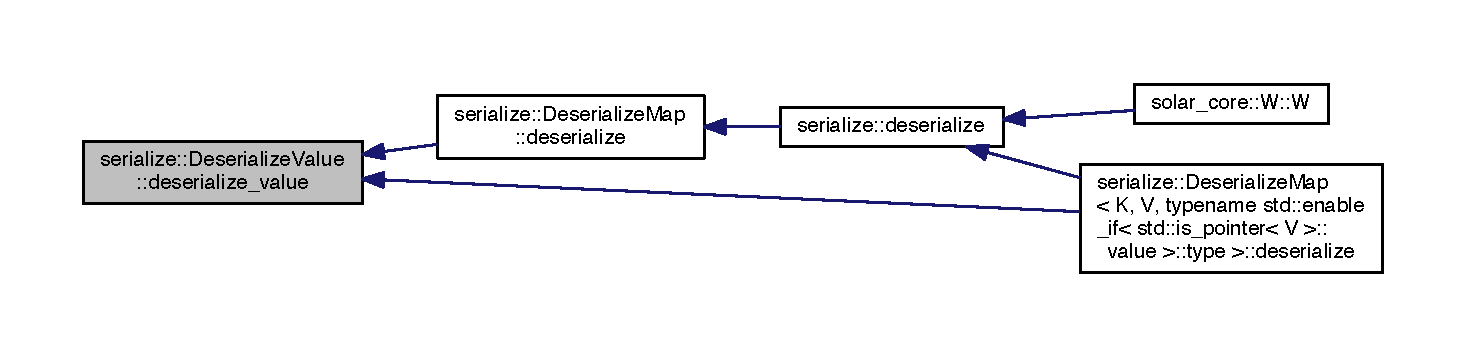
\includegraphics[width=350pt]{classserialize_1_1_deserialize_value_ae086cfe3996b96c0a82785afe0af81b1_icgraph}
\end{center}
\end{figure}


\hypertarget{classserialize_1_1_deserialize_value_a85960dc8ca3587ca9c275c0deb679bb7}{}\index{serialize\+::\+Deserialize\+Value@{serialize\+::\+Deserialize\+Value}!deserialize\+\_\+value@{deserialize\+\_\+value}}
\index{deserialize\+\_\+value@{deserialize\+\_\+value}!serialize\+::\+Deserialize\+Value@{serialize\+::\+Deserialize\+Value}}
\subsubsection[{deserialize\+\_\+value}]{\setlength{\rightskip}{0pt plus 5cm}template$<$class T , class Enable  = void$>$ static void {\bf serialize\+::\+Deserialize\+Value}$<$ T, Enable $>$\+::deserialize\+\_\+value (
\begin{DoxyParamCaption}
\item[{std\+::stringstream \&}]{ss, }
\item[{T \&}]{out\+\_\+}
\end{DoxyParamCaption}
)\hspace{0.3cm}{\ttfamily [inline]}, {\ttfamily [static]}}\label{classserialize_1_1_deserialize_value_a85960dc8ca3587ca9c275c0deb679bb7}


Definition at line 76 of file Serialize.\+h.



The documentation for this class was generated from the following file\+:\begin{DoxyCompactItemize}
\item 
/\+Users/wilfeli/\+Dropbox/\+A\+B\+M/\+Solar\+Panels/\+A\+B\+M\+I\+R\+I\+S\+Lab/\+Source/\+Tools/\hyperlink{_serialize_8h}{Serialize.\+h}\end{DoxyCompactItemize}

\hypertarget{classserialize_1_1_deserialize_value_3_01_t_00_01typename_01std_1_1enable__if_3_01std_1_1is__sambc4bb2b40dcc8b30285e8bdc35bf8b03}{}\section{serialize\+:\+:Deserialize\+Value$<$ T, typename std\+:\+:enable\+\_\+if$<$ std\+:\+:is\+\_\+same$<$ T, std\+:\+:string $>$\+:\+:value $>$\+:\+:type $>$ Class Template Reference}
\label{classserialize_1_1_deserialize_value_3_01_t_00_01typename_01std_1_1enable__if_3_01std_1_1is__sambc4bb2b40dcc8b30285e8bdc35bf8b03}\index{serialize\+::\+Deserialize\+Value$<$ T, typename std\+::enable\+\_\+if$<$ std\+::is\+\_\+same$<$ T, std\+::string $>$\+::value $>$\+::type $>$@{serialize\+::\+Deserialize\+Value$<$ T, typename std\+::enable\+\_\+if$<$ std\+::is\+\_\+same$<$ T, std\+::string $>$\+::value $>$\+::type $>$}}


{\ttfamily \#include $<$Serialize.\+h$>$}

\subsection*{Static Public Member Functions}
\begin{DoxyCompactItemize}
\item 
static void \hyperlink{classserialize_1_1_deserialize_value_3_01_t_00_01typename_01std_1_1enable__if_3_01std_1_1is__sambc4bb2b40dcc8b30285e8bdc35bf8b03_a2540f84ec617252a8ce92375fac010aa}{deserialize\+\_\+value} (const std\+::string \&in\+\_\+, T \&out\+\_\+)
\item 
static void \hyperlink{classserialize_1_1_deserialize_value_3_01_t_00_01typename_01std_1_1enable__if_3_01std_1_1is__sambc4bb2b40dcc8b30285e8bdc35bf8b03_afbc20e3c6749cfafb3c0fffe41eb4bf6}{deserialize\+\_\+value} (std\+::stringstream \&ss, T \&out\+\_\+)
\end{DoxyCompactItemize}


\subsection{Detailed Description}
\subsubsection*{template$<$class T$>$class serialize\+::\+Deserialize\+Value$<$ T, typename std\+::enable\+\_\+if$<$ std\+::is\+\_\+same$<$ T, std\+::string $>$\+::value $>$\+::type $>$}



Definition at line 84 of file Serialize.\+h.



\subsection{Member Function Documentation}
\hypertarget{classserialize_1_1_deserialize_value_3_01_t_00_01typename_01std_1_1enable__if_3_01std_1_1is__sambc4bb2b40dcc8b30285e8bdc35bf8b03_a2540f84ec617252a8ce92375fac010aa}{}\index{serialize\+::\+Deserialize\+Value$<$ T, typename std\+::enable\+\_\+if$<$ std\+::is\+\_\+same$<$ T, std\+::string $>$\+::value $>$\+::type $>$@{serialize\+::\+Deserialize\+Value$<$ T, typename std\+::enable\+\_\+if$<$ std\+::is\+\_\+same$<$ T, std\+::string $>$\+::value $>$\+::type $>$}!deserialize\+\_\+value@{deserialize\+\_\+value}}
\index{deserialize\+\_\+value@{deserialize\+\_\+value}!serialize\+::\+Deserialize\+Value$<$ T, typename std\+::enable\+\_\+if$<$ std\+::is\+\_\+same$<$ T, std\+::string $>$\+::value $>$\+::type $>$@{serialize\+::\+Deserialize\+Value$<$ T, typename std\+::enable\+\_\+if$<$ std\+::is\+\_\+same$<$ T, std\+::string $>$\+::value $>$\+::type $>$}}
\subsubsection[{deserialize\+\_\+value}]{\setlength{\rightskip}{0pt plus 5cm}template$<$class T $>$ static void {\bf serialize\+::\+Deserialize\+Value}$<$ T, typename std\+::enable\+\_\+if$<$ std\+::is\+\_\+same$<$ T, std\+::string $>$\+::value $>$\+::type $>$\+::deserialize\+\_\+value (
\begin{DoxyParamCaption}
\item[{const std\+::string \&}]{in\+\_\+, }
\item[{T \&}]{out\+\_\+}
\end{DoxyParamCaption}
)\hspace{0.3cm}{\ttfamily [inline]}, {\ttfamily [static]}}\label{classserialize_1_1_deserialize_value_3_01_t_00_01typename_01std_1_1enable__if_3_01std_1_1is__sambc4bb2b40dcc8b30285e8bdc35bf8b03_a2540f84ec617252a8ce92375fac010aa}


Definition at line 87 of file Serialize.\+h.

\hypertarget{classserialize_1_1_deserialize_value_3_01_t_00_01typename_01std_1_1enable__if_3_01std_1_1is__sambc4bb2b40dcc8b30285e8bdc35bf8b03_afbc20e3c6749cfafb3c0fffe41eb4bf6}{}\index{serialize\+::\+Deserialize\+Value$<$ T, typename std\+::enable\+\_\+if$<$ std\+::is\+\_\+same$<$ T, std\+::string $>$\+::value $>$\+::type $>$@{serialize\+::\+Deserialize\+Value$<$ T, typename std\+::enable\+\_\+if$<$ std\+::is\+\_\+same$<$ T, std\+::string $>$\+::value $>$\+::type $>$}!deserialize\+\_\+value@{deserialize\+\_\+value}}
\index{deserialize\+\_\+value@{deserialize\+\_\+value}!serialize\+::\+Deserialize\+Value$<$ T, typename std\+::enable\+\_\+if$<$ std\+::is\+\_\+same$<$ T, std\+::string $>$\+::value $>$\+::type $>$@{serialize\+::\+Deserialize\+Value$<$ T, typename std\+::enable\+\_\+if$<$ std\+::is\+\_\+same$<$ T, std\+::string $>$\+::value $>$\+::type $>$}}
\subsubsection[{deserialize\+\_\+value}]{\setlength{\rightskip}{0pt plus 5cm}template$<$class T $>$ static void {\bf serialize\+::\+Deserialize\+Value}$<$ T, typename std\+::enable\+\_\+if$<$ std\+::is\+\_\+same$<$ T, std\+::string $>$\+::value $>$\+::type $>$\+::deserialize\+\_\+value (
\begin{DoxyParamCaption}
\item[{std\+::stringstream \&}]{ss, }
\item[{T \&}]{out\+\_\+}
\end{DoxyParamCaption}
)\hspace{0.3cm}{\ttfamily [inline]}, {\ttfamily [static]}}\label{classserialize_1_1_deserialize_value_3_01_t_00_01typename_01std_1_1enable__if_3_01std_1_1is__sambc4bb2b40dcc8b30285e8bdc35bf8b03_afbc20e3c6749cfafb3c0fffe41eb4bf6}


Definition at line 93 of file Serialize.\+h.



The documentation for this class was generated from the following file\+:\begin{DoxyCompactItemize}
\item 
/\+Users/wilfeli/\+Dropbox/\+A\+B\+M/\+Solar\+Panels/\+A\+B\+M\+I\+R\+I\+S\+Lab/\+Source/\+Tools/\hyperlink{_serialize_8h}{Serialize.\+h}\end{DoxyCompactItemize}

\hypertarget{structsolar__core_1_1_world_settings_1_1_e_hash}{}\section{solar\+\_\+core\+:\+:World\+Settings\+:\+:E\+Hash Struct Reference}
\label{structsolar__core_1_1_world_settings_1_1_e_hash}\index{solar\+\_\+core\+::\+World\+Settings\+::\+E\+Hash@{solar\+\_\+core\+::\+World\+Settings\+::\+E\+Hash}}


{\ttfamily \#include $<$World\+Settings.\+h$>$}

\subsection*{Public Member Functions}
\begin{DoxyCompactItemize}
\item 
{\footnotesize template$<$typename T $>$ }\\std\+::size\+\_\+t \hyperlink{structsolar__core_1_1_world_settings_1_1_e_hash_aabc40342ca3ed6e79168a292a7b98f74}{operator()} (T t) const 
\end{DoxyCompactItemize}


\subsection{Detailed Description}
Parameteres, setting up, etc. section 

Definition at line 42 of file World\+Settings.\+h.



\subsection{Member Function Documentation}
\hypertarget{structsolar__core_1_1_world_settings_1_1_e_hash_aabc40342ca3ed6e79168a292a7b98f74}{}\index{solar\+\_\+core\+::\+World\+Settings\+::\+E\+Hash@{solar\+\_\+core\+::\+World\+Settings\+::\+E\+Hash}!operator()@{operator()}}
\index{operator()@{operator()}!solar\+\_\+core\+::\+World\+Settings\+::\+E\+Hash@{solar\+\_\+core\+::\+World\+Settings\+::\+E\+Hash}}
\subsubsection[{operator()}]{\setlength{\rightskip}{0pt plus 5cm}template$<$typename T $>$ std\+::size\+\_\+t solar\+\_\+core\+::\+World\+Settings\+::\+E\+Hash\+::operator() (
\begin{DoxyParamCaption}
\item[{T}]{t}
\end{DoxyParamCaption}
) const\hspace{0.3cm}{\ttfamily [inline]}}\label{structsolar__core_1_1_world_settings_1_1_e_hash_aabc40342ca3ed6e79168a292a7b98f74}


Definition at line 45 of file World\+Settings.\+h.



The documentation for this struct was generated from the following file\+:\begin{DoxyCompactItemize}
\item 
/\+Users/wilfeli/\+Dropbox/\+A\+B\+M/\+Solar\+Panels/\+A\+B\+M\+I\+R\+I\+S\+Lab/\+Source/\+Tools/\hyperlink{_world_settings_8h}{World\+Settings.\+h}\end{DoxyCompactItemize}

\hypertarget{classsolar__core_1_1tools_1_1_empirical_m_v_d}{}\section{solar\+\_\+core\+:\+:tools\+:\+:Empirical\+M\+V\+D Class Reference}
\label{classsolar__core_1_1tools_1_1_empirical_m_v_d}\index{solar\+\_\+core\+::tools\+::\+Empirical\+M\+V\+D@{solar\+\_\+core\+::tools\+::\+Empirical\+M\+V\+D}}


{\ttfamily \#include $<$Simulation.\+h$>$}



Collaboration diagram for solar\+\_\+core\+:\+:tools\+:\+:Empirical\+M\+V\+D\+:
\nopagebreak
\begin{figure}[H]
\begin{center}
\leavevmode
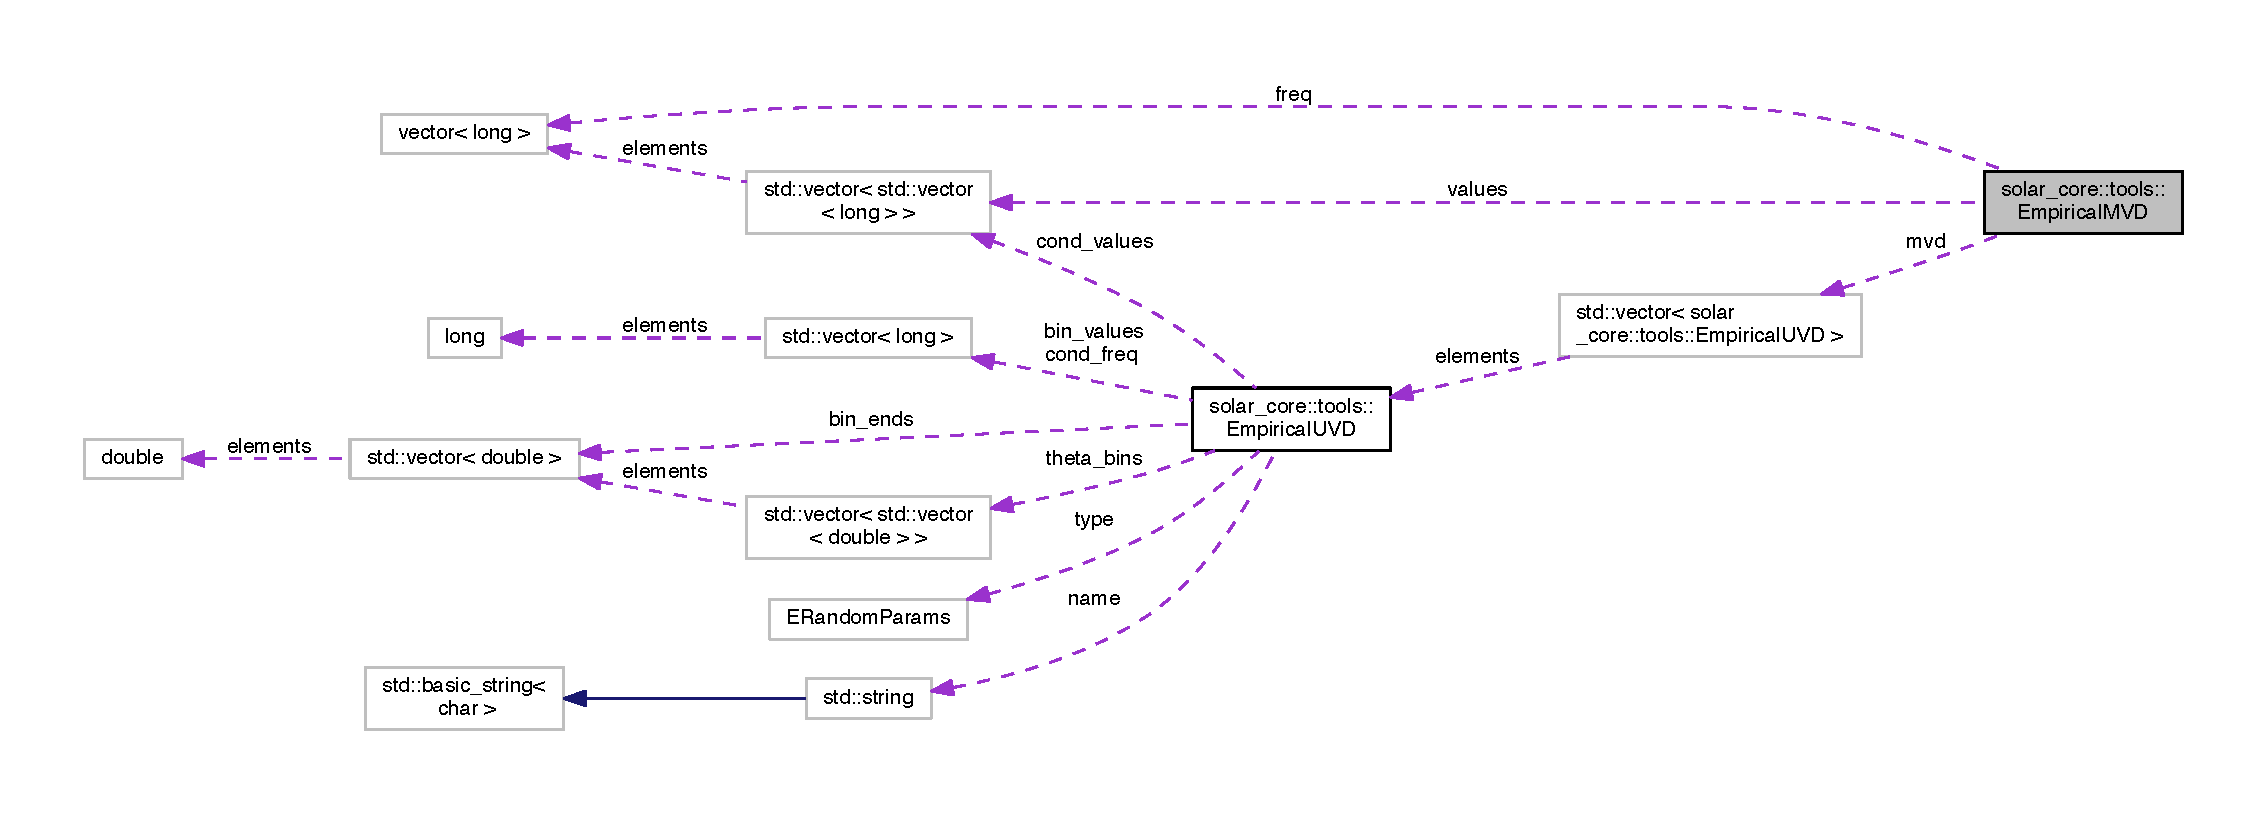
\includegraphics[width=350pt]{classsolar__core_1_1tools_1_1_empirical_m_v_d__coll__graph}
\end{center}
\end{figure}
\subsection*{Public Attributes}
\begin{DoxyCompactItemize}
\item 
std\+::vector$<$ \hyperlink{classsolar__core_1_1tools_1_1_empirical_u_v_d}{Empirical\+U\+V\+D} $>$ \hyperlink{classsolar__core_1_1tools_1_1_empirical_m_v_d_aa83e37773da6c4f70e2c7218b439ef21}{mvd}
\item 
std\+::vector$<$ std\+::vector$<$ long $>$ $>$ \hyperlink{classsolar__core_1_1tools_1_1_empirical_m_v_d_ac5fe45bde609ac9cc2dd6d3e7121ce48}{values}
\item 
std\+::vector$<$ long $>$ \hyperlink{classsolar__core_1_1tools_1_1_empirical_m_v_d_a637f45117b7ed5d52beac351440c3805}{freq}
\end{DoxyCompactItemize}


\subsection{Detailed Description}
Empirical multi-\/variate distribution 

Definition at line 62 of file Simulation.\+h.



\subsection{Member Data Documentation}
\hypertarget{classsolar__core_1_1tools_1_1_empirical_m_v_d_a637f45117b7ed5d52beac351440c3805}{}\index{solar\+\_\+core\+::tools\+::\+Empirical\+M\+V\+D@{solar\+\_\+core\+::tools\+::\+Empirical\+M\+V\+D}!freq@{freq}}
\index{freq@{freq}!solar\+\_\+core\+::tools\+::\+Empirical\+M\+V\+D@{solar\+\_\+core\+::tools\+::\+Empirical\+M\+V\+D}}
\subsubsection[{freq}]{\setlength{\rightskip}{0pt plus 5cm}std\+::vector$<$long$>$ solar\+\_\+core\+::tools\+::\+Empirical\+M\+V\+D\+::freq}\label{classsolar__core_1_1tools_1_1_empirical_m_v_d_a637f45117b7ed5d52beac351440c3805}


Definition at line 67 of file Simulation.\+h.

\hypertarget{classsolar__core_1_1tools_1_1_empirical_m_v_d_aa83e37773da6c4f70e2c7218b439ef21}{}\index{solar\+\_\+core\+::tools\+::\+Empirical\+M\+V\+D@{solar\+\_\+core\+::tools\+::\+Empirical\+M\+V\+D}!mvd@{mvd}}
\index{mvd@{mvd}!solar\+\_\+core\+::tools\+::\+Empirical\+M\+V\+D@{solar\+\_\+core\+::tools\+::\+Empirical\+M\+V\+D}}
\subsubsection[{mvd}]{\setlength{\rightskip}{0pt plus 5cm}std\+::vector$<${\bf Empirical\+U\+V\+D}$>$ solar\+\_\+core\+::tools\+::\+Empirical\+M\+V\+D\+::mvd}\label{classsolar__core_1_1tools_1_1_empirical_m_v_d_aa83e37773da6c4f70e2c7218b439ef21}


Definition at line 65 of file Simulation.\+h.

\hypertarget{classsolar__core_1_1tools_1_1_empirical_m_v_d_ac5fe45bde609ac9cc2dd6d3e7121ce48}{}\index{solar\+\_\+core\+::tools\+::\+Empirical\+M\+V\+D@{solar\+\_\+core\+::tools\+::\+Empirical\+M\+V\+D}!values@{values}}
\index{values@{values}!solar\+\_\+core\+::tools\+::\+Empirical\+M\+V\+D@{solar\+\_\+core\+::tools\+::\+Empirical\+M\+V\+D}}
\subsubsection[{values}]{\setlength{\rightskip}{0pt plus 5cm}std\+::vector$<$std\+::vector$<$long$>$ $>$ solar\+\_\+core\+::tools\+::\+Empirical\+M\+V\+D\+::values}\label{classsolar__core_1_1tools_1_1_empirical_m_v_d_ac5fe45bde609ac9cc2dd6d3e7121ce48}


Definition at line 66 of file Simulation.\+h.



The documentation for this class was generated from the following file\+:\begin{DoxyCompactItemize}
\item 
/\+Users/wilfeli/\+Dropbox/\+A\+B\+M/\+Solar\+Panels/\+A\+B\+M\+I\+R\+I\+S\+Lab/\+Source/\+Tools/\hyperlink{_simulation_8h}{Simulation.\+h}\end{DoxyCompactItemize}

\hypertarget{classsolar__core_1_1tools_1_1_empirical_u_v_d}{}\section{solar\+\_\+core\+:\+:tools\+:\+:Empirical\+U\+V\+D Class Reference}
\label{classsolar__core_1_1tools_1_1_empirical_u_v_d}\index{solar\+\_\+core\+::tools\+::\+Empirical\+U\+V\+D@{solar\+\_\+core\+::tools\+::\+Empirical\+U\+V\+D}}


{\ttfamily \#include $<$Simulation.\+h$>$}



Collaboration diagram for solar\+\_\+core\+:\+:tools\+:\+:Empirical\+U\+V\+D\+:
\nopagebreak
\begin{figure}[H]
\begin{center}
\leavevmode
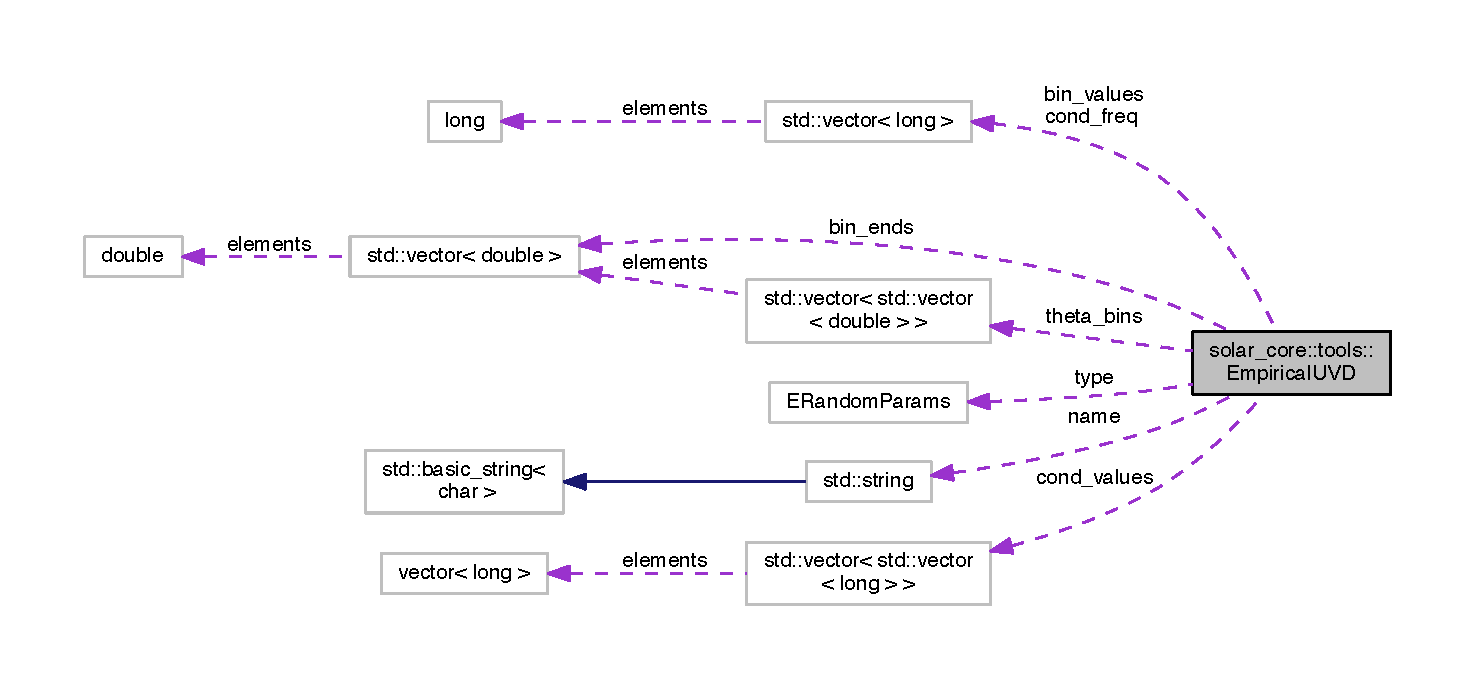
\includegraphics[width=350pt]{classsolar__core_1_1tools_1_1_empirical_u_v_d__coll__graph}
\end{center}
\end{figure}
\subsection*{Public Member Functions}
\begin{DoxyCompactItemize}
\item 
\hyperlink{classsolar__core_1_1tools_1_1_empirical_u_v_d_a3745b987a8d7c7e61d2aabbaf652a3e5}{Empirical\+U\+V\+D} ()=default
\end{DoxyCompactItemize}
\subsection*{Public Attributes}
\begin{DoxyCompactItemize}
\item 
std\+::string \hyperlink{classsolar__core_1_1tools_1_1_empirical_u_v_d_a4f2500cdf861542aa18c417564f43762}{name}
\item 
\hyperlink{namespacesolar__core_a1a8e58483c0cf418bd680fc3a0ca8222}{E\+Random\+Params} \hyperlink{classsolar__core_1_1tools_1_1_empirical_u_v_d_a581e5c7f2116d67f5a250725624ff908}{type}
\item 
std\+::vector$<$ double $>$ \hyperlink{classsolar__core_1_1tools_1_1_empirical_u_v_d_aa0a0775b7b188d292a98e91c3bd8a1b5}{bin\+\_\+ends}
\item 
std\+::vector$<$ long $>$ \hyperlink{classsolar__core_1_1tools_1_1_empirical_u_v_d_a88761616541a12ec55dc74fea5613377}{bin\+\_\+values}
\item 
std\+::vector$<$ std\+::vector$<$ long $>$ $>$ \hyperlink{classsolar__core_1_1tools_1_1_empirical_u_v_d_a51ef33f87ed7836a5239c39e8466efc6}{cond\+\_\+values}
\item 
std\+::vector$<$ long $>$ \hyperlink{classsolar__core_1_1tools_1_1_empirical_u_v_d_a19135ba9bf7bb2c5c5819964e6149b2c}{cond\+\_\+freq}
\item 
std\+::vector$<$ std\+::vector$<$ double $>$ $>$ \hyperlink{classsolar__core_1_1tools_1_1_empirical_u_v_d_aa5c9e49cc6e7b7788f9f14256a83d76f}{theta\+\_\+bins}
\end{DoxyCompactItemize}


\subsection{Detailed Description}
Empirical univariate distribution 

Definition at line 38 of file Simulation.\+h.



\subsection{Constructor \& Destructor Documentation}
\hypertarget{classsolar__core_1_1tools_1_1_empirical_u_v_d_a3745b987a8d7c7e61d2aabbaf652a3e5}{}\index{solar\+\_\+core\+::tools\+::\+Empirical\+U\+V\+D@{solar\+\_\+core\+::tools\+::\+Empirical\+U\+V\+D}!Empirical\+U\+V\+D@{Empirical\+U\+V\+D}}
\index{Empirical\+U\+V\+D@{Empirical\+U\+V\+D}!solar\+\_\+core\+::tools\+::\+Empirical\+U\+V\+D@{solar\+\_\+core\+::tools\+::\+Empirical\+U\+V\+D}}
\subsubsection[{Empirical\+U\+V\+D}]{\setlength{\rightskip}{0pt plus 5cm}solar\+\_\+core\+::tools\+::\+Empirical\+U\+V\+D\+::\+Empirical\+U\+V\+D (
\begin{DoxyParamCaption}
{}
\end{DoxyParamCaption}
)\hspace{0.3cm}{\ttfamily [default]}}\label{classsolar__core_1_1tools_1_1_empirical_u_v_d_a3745b987a8d7c7e61d2aabbaf652a3e5}


\subsection{Member Data Documentation}
\hypertarget{classsolar__core_1_1tools_1_1_empirical_u_v_d_aa0a0775b7b188d292a98e91c3bd8a1b5}{}\index{solar\+\_\+core\+::tools\+::\+Empirical\+U\+V\+D@{solar\+\_\+core\+::tools\+::\+Empirical\+U\+V\+D}!bin\+\_\+ends@{bin\+\_\+ends}}
\index{bin\+\_\+ends@{bin\+\_\+ends}!solar\+\_\+core\+::tools\+::\+Empirical\+U\+V\+D@{solar\+\_\+core\+::tools\+::\+Empirical\+U\+V\+D}}
\subsubsection[{bin\+\_\+ends}]{\setlength{\rightskip}{0pt plus 5cm}std\+::vector$<$double$>$ solar\+\_\+core\+::tools\+::\+Empirical\+U\+V\+D\+::bin\+\_\+ends}\label{classsolar__core_1_1tools_1_1_empirical_u_v_d_aa0a0775b7b188d292a98e91c3bd8a1b5}


Definition at line 44 of file Simulation.\+h.

\hypertarget{classsolar__core_1_1tools_1_1_empirical_u_v_d_a88761616541a12ec55dc74fea5613377}{}\index{solar\+\_\+core\+::tools\+::\+Empirical\+U\+V\+D@{solar\+\_\+core\+::tools\+::\+Empirical\+U\+V\+D}!bin\+\_\+values@{bin\+\_\+values}}
\index{bin\+\_\+values@{bin\+\_\+values}!solar\+\_\+core\+::tools\+::\+Empirical\+U\+V\+D@{solar\+\_\+core\+::tools\+::\+Empirical\+U\+V\+D}}
\subsubsection[{bin\+\_\+values}]{\setlength{\rightskip}{0pt plus 5cm}std\+::vector$<$long$>$ solar\+\_\+core\+::tools\+::\+Empirical\+U\+V\+D\+::bin\+\_\+values}\label{classsolar__core_1_1tools_1_1_empirical_u_v_d_a88761616541a12ec55dc74fea5613377}


Definition at line 45 of file Simulation.\+h.

\hypertarget{classsolar__core_1_1tools_1_1_empirical_u_v_d_a19135ba9bf7bb2c5c5819964e6149b2c}{}\index{solar\+\_\+core\+::tools\+::\+Empirical\+U\+V\+D@{solar\+\_\+core\+::tools\+::\+Empirical\+U\+V\+D}!cond\+\_\+freq@{cond\+\_\+freq}}
\index{cond\+\_\+freq@{cond\+\_\+freq}!solar\+\_\+core\+::tools\+::\+Empirical\+U\+V\+D@{solar\+\_\+core\+::tools\+::\+Empirical\+U\+V\+D}}
\subsubsection[{cond\+\_\+freq}]{\setlength{\rightskip}{0pt plus 5cm}std\+::vector$<$long$>$ solar\+\_\+core\+::tools\+::\+Empirical\+U\+V\+D\+::cond\+\_\+freq}\label{classsolar__core_1_1tools_1_1_empirical_u_v_d_a19135ba9bf7bb2c5c5819964e6149b2c}


Definition at line 48 of file Simulation.\+h.

\hypertarget{classsolar__core_1_1tools_1_1_empirical_u_v_d_a51ef33f87ed7836a5239c39e8466efc6}{}\index{solar\+\_\+core\+::tools\+::\+Empirical\+U\+V\+D@{solar\+\_\+core\+::tools\+::\+Empirical\+U\+V\+D}!cond\+\_\+values@{cond\+\_\+values}}
\index{cond\+\_\+values@{cond\+\_\+values}!solar\+\_\+core\+::tools\+::\+Empirical\+U\+V\+D@{solar\+\_\+core\+::tools\+::\+Empirical\+U\+V\+D}}
\subsubsection[{cond\+\_\+values}]{\setlength{\rightskip}{0pt plus 5cm}std\+::vector$<$std\+::vector$<$long$>$ $>$ solar\+\_\+core\+::tools\+::\+Empirical\+U\+V\+D\+::cond\+\_\+values}\label{classsolar__core_1_1tools_1_1_empirical_u_v_d_a51ef33f87ed7836a5239c39e8466efc6}


Definition at line 47 of file Simulation.\+h.

\hypertarget{classsolar__core_1_1tools_1_1_empirical_u_v_d_a4f2500cdf861542aa18c417564f43762}{}\index{solar\+\_\+core\+::tools\+::\+Empirical\+U\+V\+D@{solar\+\_\+core\+::tools\+::\+Empirical\+U\+V\+D}!name@{name}}
\index{name@{name}!solar\+\_\+core\+::tools\+::\+Empirical\+U\+V\+D@{solar\+\_\+core\+::tools\+::\+Empirical\+U\+V\+D}}
\subsubsection[{name}]{\setlength{\rightskip}{0pt plus 5cm}std\+::string solar\+\_\+core\+::tools\+::\+Empirical\+U\+V\+D\+::name}\label{classsolar__core_1_1tools_1_1_empirical_u_v_d_a4f2500cdf861542aa18c417564f43762}


Definition at line 42 of file Simulation.\+h.

\hypertarget{classsolar__core_1_1tools_1_1_empirical_u_v_d_aa5c9e49cc6e7b7788f9f14256a83d76f}{}\index{solar\+\_\+core\+::tools\+::\+Empirical\+U\+V\+D@{solar\+\_\+core\+::tools\+::\+Empirical\+U\+V\+D}!theta\+\_\+bins@{theta\+\_\+bins}}
\index{theta\+\_\+bins@{theta\+\_\+bins}!solar\+\_\+core\+::tools\+::\+Empirical\+U\+V\+D@{solar\+\_\+core\+::tools\+::\+Empirical\+U\+V\+D}}
\subsubsection[{theta\+\_\+bins}]{\setlength{\rightskip}{0pt plus 5cm}std\+::vector$<$std\+::vector$<$double$>$ $>$ solar\+\_\+core\+::tools\+::\+Empirical\+U\+V\+D\+::theta\+\_\+bins}\label{classsolar__core_1_1tools_1_1_empirical_u_v_d_aa5c9e49cc6e7b7788f9f14256a83d76f}


Definition at line 50 of file Simulation.\+h.

\hypertarget{classsolar__core_1_1tools_1_1_empirical_u_v_d_a581e5c7f2116d67f5a250725624ff908}{}\index{solar\+\_\+core\+::tools\+::\+Empirical\+U\+V\+D@{solar\+\_\+core\+::tools\+::\+Empirical\+U\+V\+D}!type@{type}}
\index{type@{type}!solar\+\_\+core\+::tools\+::\+Empirical\+U\+V\+D@{solar\+\_\+core\+::tools\+::\+Empirical\+U\+V\+D}}
\subsubsection[{type}]{\setlength{\rightskip}{0pt plus 5cm}{\bf E\+Random\+Params} solar\+\_\+core\+::tools\+::\+Empirical\+U\+V\+D\+::type}\label{classsolar__core_1_1tools_1_1_empirical_u_v_d_a581e5c7f2116d67f5a250725624ff908}


Definition at line 43 of file Simulation.\+h.



The documentation for this class was generated from the following file\+:\begin{DoxyCompactItemize}
\item 
/\+Users/wilfeli/\+Dropbox/\+A\+B\+M/\+Solar\+Panels/\+A\+B\+M\+I\+R\+I\+S\+Lab/\+Source/\+Tools/\hyperlink{_simulation_8h}{Simulation.\+h}\end{DoxyCompactItemize}

\hypertarget{classsolar__core_1_1_enum_factory}{}\section{solar\+\_\+core\+:\+:Enum\+Factory Class Reference}
\label{classsolar__core_1_1_enum_factory}\index{solar\+\_\+core\+::\+Enum\+Factory@{solar\+\_\+core\+::\+Enum\+Factory}}


{\ttfamily \#include $<$I\+Parameters.\+h$>$}

\subsection*{Static Public Member Functions}
\begin{DoxyCompactItemize}
\item 
static \hyperlink{namespacesolar__core_aa1147341e5ef7a40d68d1bd68e149362}{E\+Param\+Types} \hyperlink{classsolar__core_1_1_enum_factory_a573986ee0b4951d5ecc6a8c100f892e8}{To\+E\+Param\+Types} (std\+::string param\+\_\+type)
\item 
static std\+::string \hyperlink{classsolar__core_1_1_enum_factory_a7f31a62dd221ed41128618d9eb74b4ee}{From\+E\+Param\+Types} (\hyperlink{namespacesolar__core_aa1147341e5ef7a40d68d1bd68e149362}{E\+Param\+Types} param\+\_\+)
\item 
static \hyperlink{namespacesolar__core_ac827fdef4412a3c0d5e44d3f31908e49}{E\+Constraint\+Params} \hyperlink{classsolar__core_1_1_enum_factory_a1763c822c6b7da0b574ef80045cd59a8}{To\+E\+Constraint\+Params} (std\+::string param\+\_\+type)
\end{DoxyCompactItemize}


\subsection{Detailed Description}


Definition at line 422 of file I\+Parameters.\+h.



\subsection{Member Function Documentation}
\hypertarget{classsolar__core_1_1_enum_factory_a7f31a62dd221ed41128618d9eb74b4ee}{}\index{solar\+\_\+core\+::\+Enum\+Factory@{solar\+\_\+core\+::\+Enum\+Factory}!From\+E\+Param\+Types@{From\+E\+Param\+Types}}
\index{From\+E\+Param\+Types@{From\+E\+Param\+Types}!solar\+\_\+core\+::\+Enum\+Factory@{solar\+\_\+core\+::\+Enum\+Factory}}
\subsubsection[{From\+E\+Param\+Types}]{\setlength{\rightskip}{0pt plus 5cm}static std\+::string solar\+\_\+core\+::\+Enum\+Factory\+::\+From\+E\+Param\+Types (
\begin{DoxyParamCaption}
\item[{{\bf E\+Param\+Types}}]{param\+\_\+}
\end{DoxyParamCaption}
)\hspace{0.3cm}{\ttfamily [inline]}, {\ttfamily [static]}}\label{classsolar__core_1_1_enum_factory_a7f31a62dd221ed41128618d9eb74b4ee}


Definition at line 605 of file I\+Parameters.\+h.



Here is the caller graph for this function\+:
\nopagebreak
\begin{figure}[H]
\begin{center}
\leavevmode
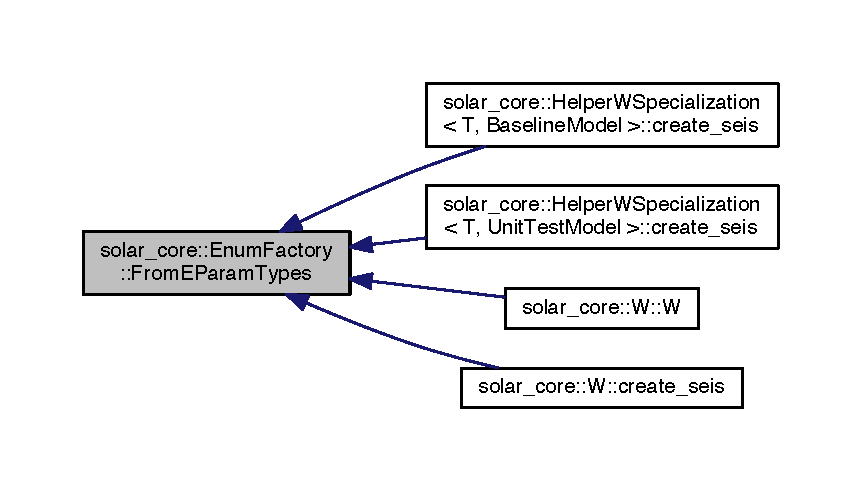
\includegraphics[width=350pt]{classsolar__core_1_1_enum_factory_a7f31a62dd221ed41128618d9eb74b4ee_icgraph}
\end{center}
\end{figure}


\hypertarget{classsolar__core_1_1_enum_factory_a1763c822c6b7da0b574ef80045cd59a8}{}\index{solar\+\_\+core\+::\+Enum\+Factory@{solar\+\_\+core\+::\+Enum\+Factory}!To\+E\+Constraint\+Params@{To\+E\+Constraint\+Params}}
\index{To\+E\+Constraint\+Params@{To\+E\+Constraint\+Params}!solar\+\_\+core\+::\+Enum\+Factory@{solar\+\_\+core\+::\+Enum\+Factory}}
\subsubsection[{To\+E\+Constraint\+Params}]{\setlength{\rightskip}{0pt plus 5cm}static {\bf E\+Constraint\+Params} solar\+\_\+core\+::\+Enum\+Factory\+::\+To\+E\+Constraint\+Params (
\begin{DoxyParamCaption}
\item[{std\+::string}]{param\+\_\+type}
\end{DoxyParamCaption}
)\hspace{0.3cm}{\ttfamily [inline]}, {\ttfamily [static]}}\label{classsolar__core_1_1_enum_factory_a1763c822c6b7da0b574ef80045cd59a8}


Definition at line 640 of file I\+Parameters.\+h.



Here is the caller graph for this function\+:
\nopagebreak
\begin{figure}[H]
\begin{center}
\leavevmode
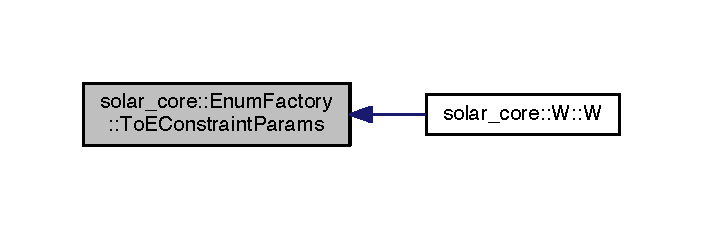
\includegraphics[width=338pt]{classsolar__core_1_1_enum_factory_a1763c822c6b7da0b574ef80045cd59a8_icgraph}
\end{center}
\end{figure}


\hypertarget{classsolar__core_1_1_enum_factory_a573986ee0b4951d5ecc6a8c100f892e8}{}\index{solar\+\_\+core\+::\+Enum\+Factory@{solar\+\_\+core\+::\+Enum\+Factory}!To\+E\+Param\+Types@{To\+E\+Param\+Types}}
\index{To\+E\+Param\+Types@{To\+E\+Param\+Types}!solar\+\_\+core\+::\+Enum\+Factory@{solar\+\_\+core\+::\+Enum\+Factory}}
\subsubsection[{To\+E\+Param\+Types}]{\setlength{\rightskip}{0pt plus 5cm}static {\bf E\+Param\+Types} solar\+\_\+core\+::\+Enum\+Factory\+::\+To\+E\+Param\+Types (
\begin{DoxyParamCaption}
\item[{std\+::string}]{param\+\_\+type}
\end{DoxyParamCaption}
)\hspace{0.3cm}{\ttfamily [inline]}, {\ttfamily [static]}}\label{classsolar__core_1_1_enum_factory_a573986ee0b4951d5ecc6a8c100f892e8}


Definition at line 424 of file I\+Parameters.\+h.



Here is the caller graph for this function\+:
\nopagebreak
\begin{figure}[H]
\begin{center}
\leavevmode
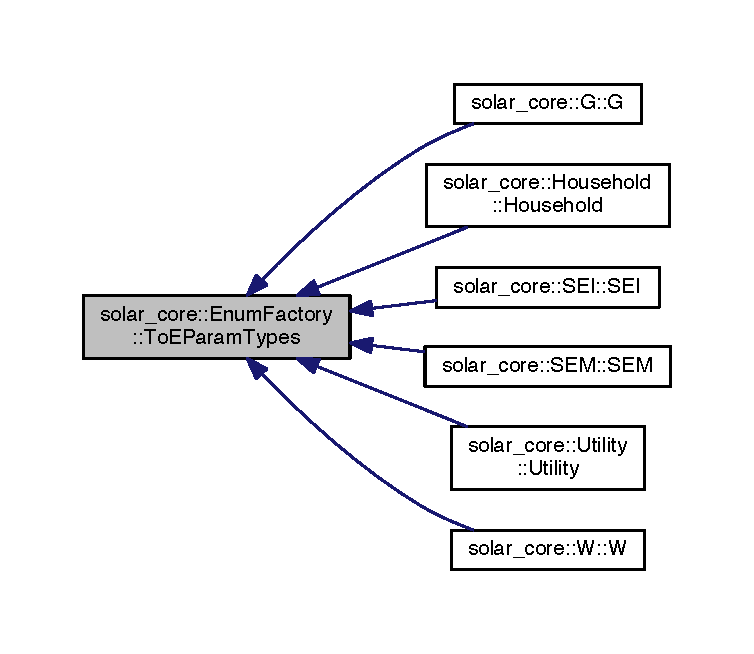
\includegraphics[width=350pt]{classsolar__core_1_1_enum_factory_a573986ee0b4951d5ecc6a8c100f892e8_icgraph}
\end{center}
\end{figure}




The documentation for this class was generated from the following file\+:\begin{DoxyCompactItemize}
\item 
/\+Users/wilfeli/\+Dropbox/\+A\+B\+M/\+Solar\+Panels/\+A\+B\+M\+I\+R\+I\+S\+Lab/\+Source/\+Tools/\hyperlink{_i_parameters_8h}{I\+Parameters.\+h}\end{DoxyCompactItemize}

\hypertarget{classsolar__core_1_1_g}{}\section{solar\+\_\+core\+:\+:G Class Reference}
\label{classsolar__core_1_1_g}\index{solar\+\_\+core\+::\+G@{solar\+\_\+core\+::\+G}}


{\ttfamily \#include $<$G.\+h$>$}



Collaboration diagram for solar\+\_\+core\+:\+:G\+:
\nopagebreak
\begin{figure}[H]
\begin{center}
\leavevmode
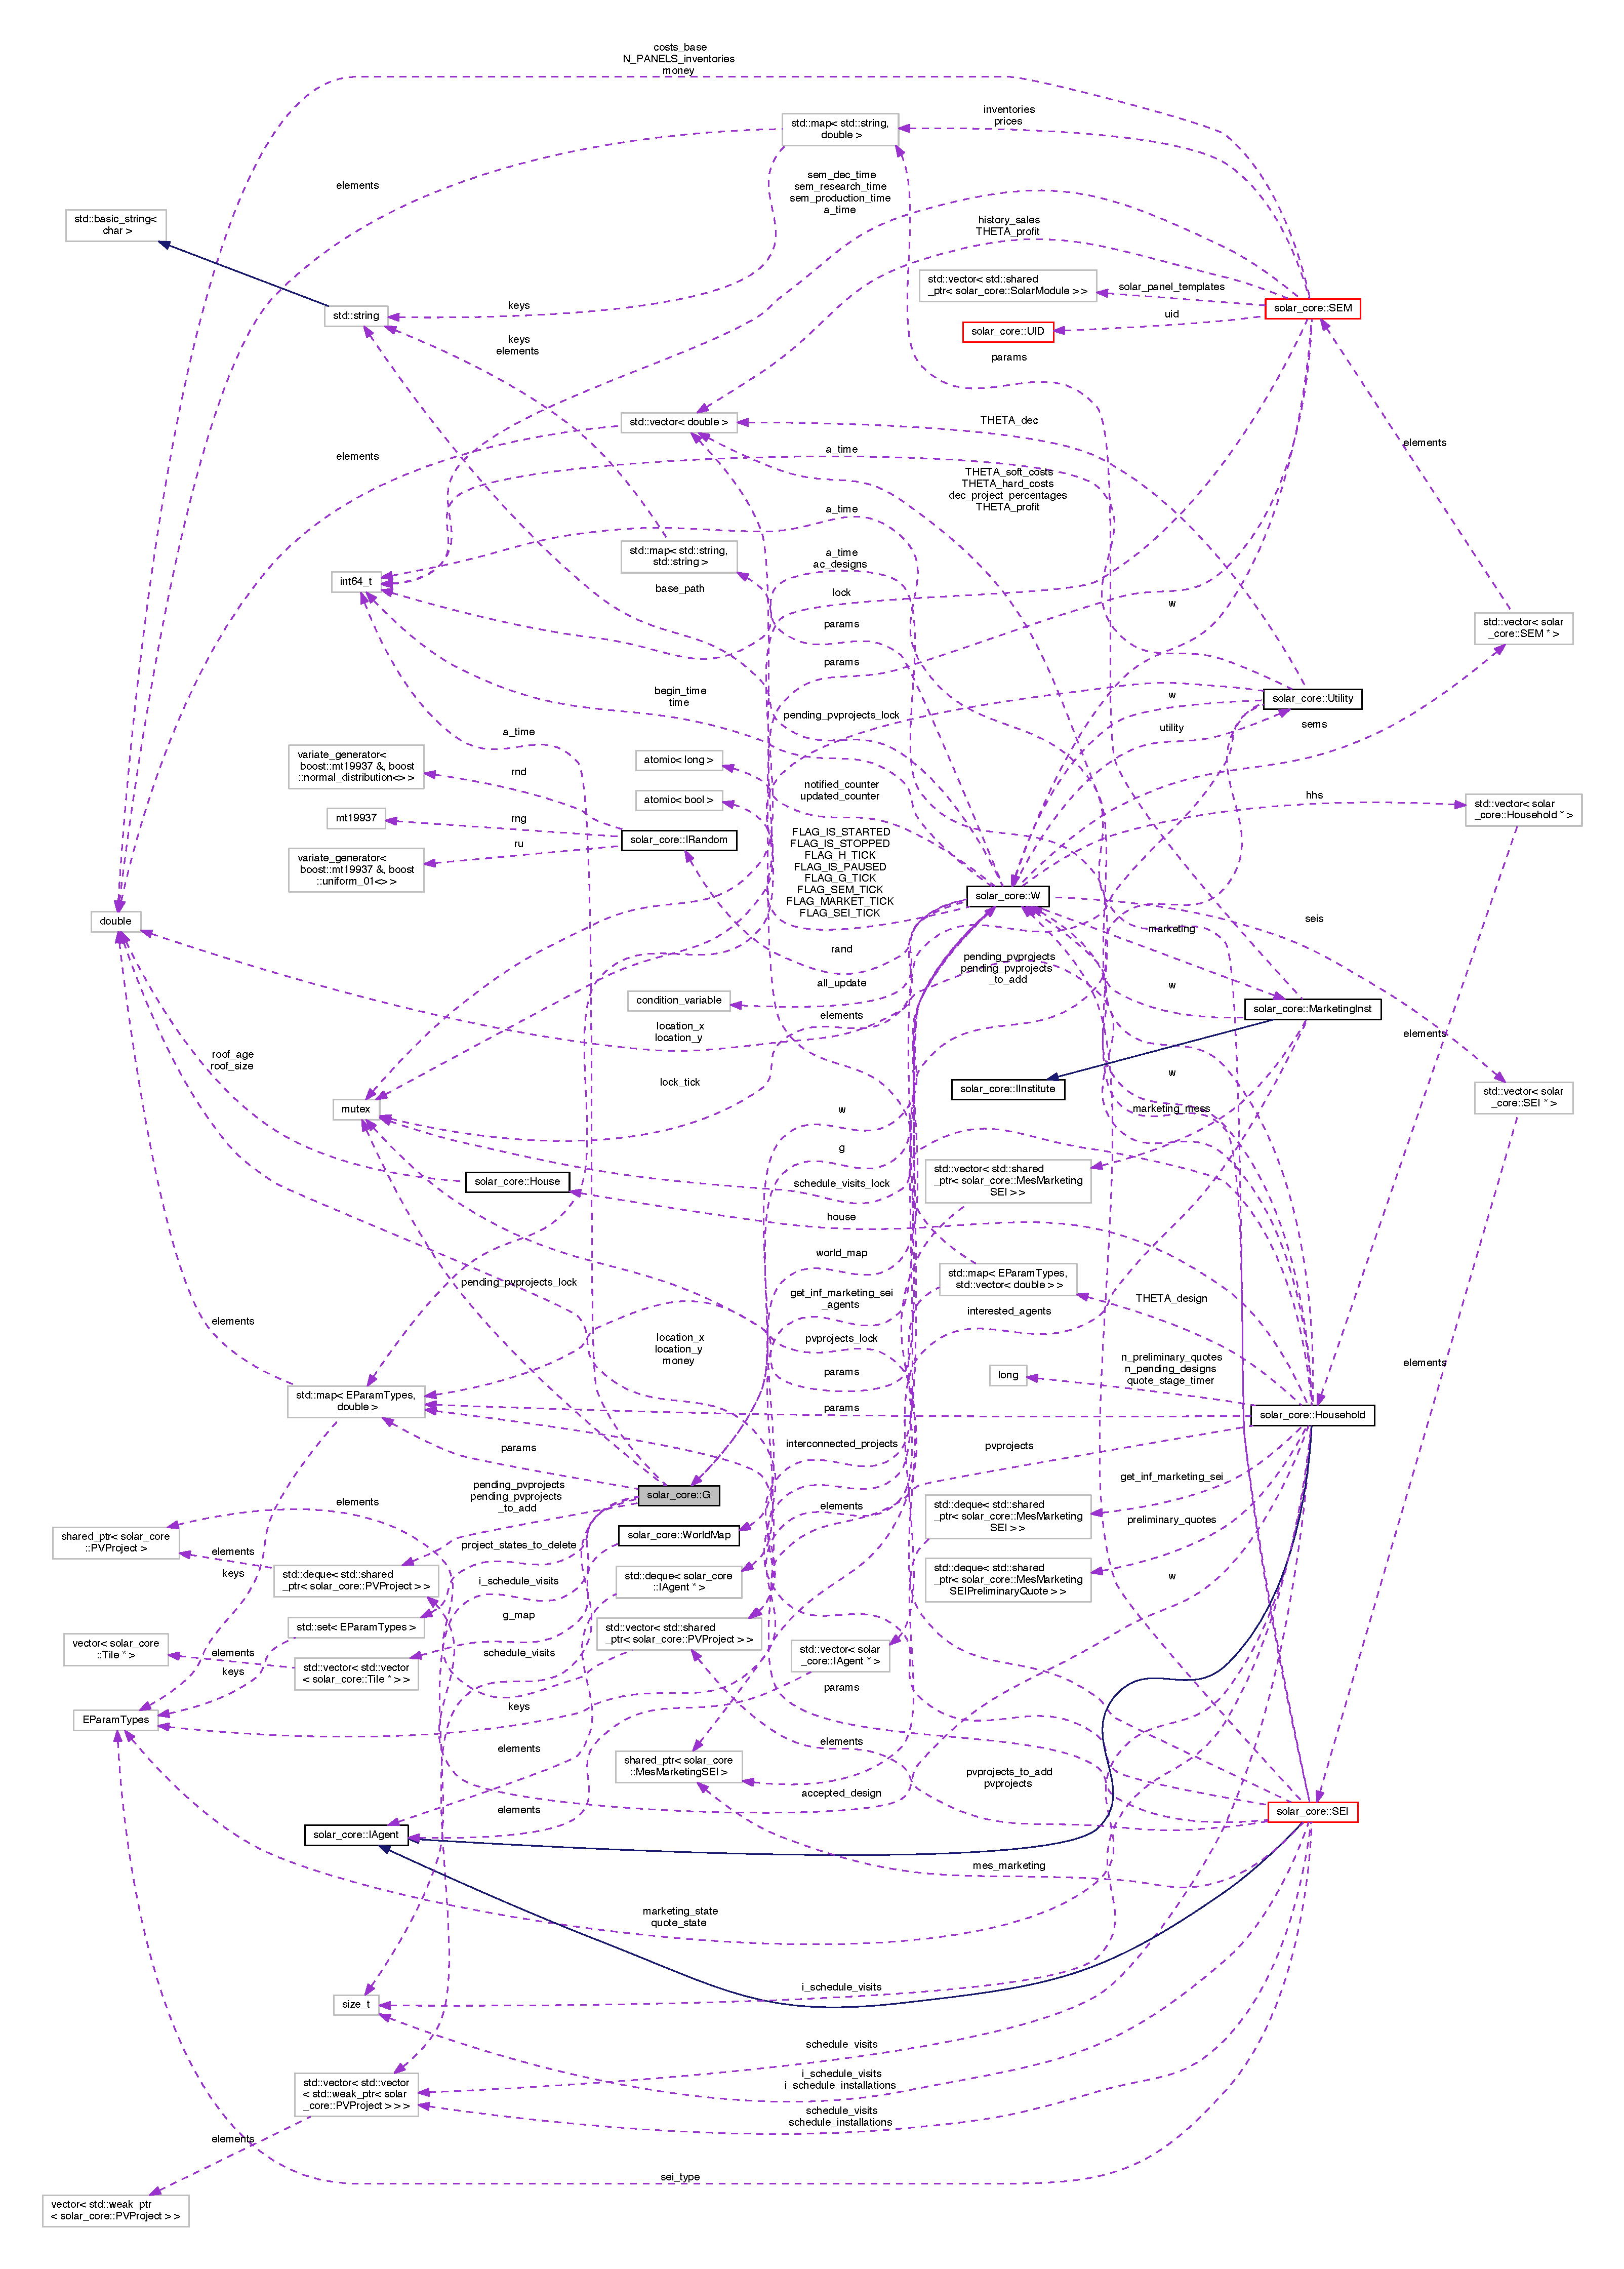
\includegraphics[height=550pt]{classsolar__core_1_1_g__coll__graph}
\end{center}
\end{figure}
\subsection*{Public Member Functions}
{\bf }\par
\begin{DoxyCompactItemize}
\item 
\hyperlink{classsolar__core_1_1_g_a624adac31ade604e0335717bad4fc9cd}{G} (const \hyperlink{namespacesolar__core_adeda2737d6938c190eb774a5b2495045}{Property\+Tree} \&pt\+\_\+, \hyperlink{classsolar__core_1_1_w}{W} $\ast$w\+\_\+)
\item 
void \hyperlink{classsolar__core_1_1_g_a0734da633e88ea0f6ff782d4b6521c09}{init} (\hyperlink{classsolar__core_1_1_w}{W} $\ast$w\+\_\+)
\item 
virtual void \hyperlink{classsolar__core_1_1_g_ad3c9fb1da4db51b296c29a6b94b0f139}{act\+\_\+tick} ()
\end{DoxyCompactItemize}

{\bf }\par
\begin{DoxyCompactItemize}
\item 
virtual void \hyperlink{classsolar__core_1_1_g_a615600f35d73a38ea48e99909fff5085}{request\+\_\+permit\+\_\+for\+\_\+installation} (std\+::shared\+\_\+ptr$<$ \hyperlink{classsolar__core_1_1_p_v_project}{P\+V\+Project} $>$ project\+\_\+)
\item 
void \hyperlink{classsolar__core_1_1_g_ae5836aff26a74e47cd26081fb94641bb}{request\+\_\+inspection} (std\+::shared\+\_\+ptr$<$ \hyperlink{classsolar__core_1_1_p_v_project}{P\+V\+Project} $>$ project\+\_\+)
\end{DoxyCompactItemize}

\begin{DoxyCompactItemize}
\item 
std\+::deque$<$ std\+::shared\+\_\+ptr$<$ \hyperlink{classsolar__core_1_1_p_v_project}{P\+V\+Project} $>$ $>$ \hyperlink{classsolar__core_1_1_g_a3a87f9e5c14cd5bae4be8a4da538181e}{pending\+\_\+pvprojects}
\item 
std\+::deque$<$ std\+::shared\+\_\+ptr$<$ \hyperlink{classsolar__core_1_1_p_v_project}{P\+V\+Project} $>$ $>$ \hyperlink{classsolar__core_1_1_g_a053a3d2c00c5af66925ebe359c4b4228}{pending\+\_\+pvprojects\+\_\+to\+\_\+add}
\item 
std\+::mutex \hyperlink{classsolar__core_1_1_g_a7ae124e062dbd50b0da66f34c9633965}{pending\+\_\+pvprojects\+\_\+lock}
\item 
std\+::vector$<$ std\+::vector$<$ std\+::weak\+\_\+ptr$<$ \hyperlink{classsolar__core_1_1_p_v_project}{P\+V\+Project} $>$ $>$ $>$ \hyperlink{classsolar__core_1_1_g_a33472d3b331a303ec8a9b61e2da163d3}{schedule\+\_\+visits}
\item 
std\+::size\+\_\+t \hyperlink{classsolar__core_1_1_g_a5c79440fcadc7d3e9212c5e7c05f84f7}{i\+\_\+schedule\+\_\+visits}
\item 
std\+::set$<$ \hyperlink{namespacesolar__core_aa1147341e5ef7a40d68d1bd68e149362}{E\+Param\+Types} $>$ \hyperlink{classsolar__core_1_1_g_a26b220870264c1927d282dfe9412725e}{project\+\_\+states\+\_\+to\+\_\+delete}
\item 
void \hyperlink{classsolar__core_1_1_g_aecc948919b4cadba36d15b458eb0b7c3}{collect\+\_\+inf\+\_\+site\+\_\+visit} (std\+::shared\+\_\+ptr$<$ \hyperlink{classsolar__core_1_1_p_v_project}{P\+V\+Project} $>$ project\+\_\+)
\item 
void \hyperlink{classsolar__core_1_1_g_af7498122edc4bfda69724fbd1d59c53d}{approve\+\_\+permit} (std\+::shared\+\_\+ptr$<$ \hyperlink{classsolar__core_1_1_p_v_project}{P\+V\+Project} $>$ project\+\_\+)
\end{DoxyCompactItemize}
\begin{DoxyCompactItemize}
\item 
std\+::map$<$ \hyperlink{namespacesolar__core_aa1147341e5ef7a40d68d1bd68e149362}{E\+Param\+Types}, double $>$ \hyperlink{classsolar__core_1_1_g_a045f1db40b15301ed5ec8aefb5327b0e}{params}
\item 
\hyperlink{classsolar__core_1_1_w}{W} $\ast$ \hyperlink{classsolar__core_1_1_g_a7239d05d617261f97c46b641a0229c14}{w}
\item 
\hyperlink{namespacesolar__core_a4b5949d07259da6f8a20d12a30403e90}{Time\+Unit} \hyperlink{classsolar__core_1_1_g_a4d5b2845fc790c0f14b13fe922821f4b}{a\+\_\+time}
\item 
void \hyperlink{classsolar__core_1_1_g_ae01d6ea43c397cc79356884c98caf277}{ac\+\_\+update\+\_\+tick} ()
\end{DoxyCompactItemize}


\subsection{Detailed Description}
There are two separate permit process, one for general permit one for interconnection. Could model it by having the probability of passing the inspection.


\begin{DoxyEnumerate}
\item permit to install 2. install 3. request for inspection 4. inspection -\/ pass or fail 5. apply for interconnection if pass 6. pass or not interconnection -\/ variable time depending on 7.
\end{DoxyEnumerate}

\hyperlink{classsolar__core_1_1_utility}{Utility} -\/ param -\/ already connected amount of energy, param -\/ potential amount of energy that could be connected (also add inflation to that), chances of connecting will depend on the difference between the two.

Degradation of P\+V -\/ 0.\+5\% per year

Check that payment is before or after installation 

Definition at line 39 of file G.\+h.



\subsection{Constructor \& Destructor Documentation}
\hypertarget{classsolar__core_1_1_g_a624adac31ade604e0335717bad4fc9cd}{}\index{solar\+\_\+core\+::\+G@{solar\+\_\+core\+::\+G}!G@{G}}
\index{G@{G}!solar\+\_\+core\+::\+G@{solar\+\_\+core\+::\+G}}
\subsubsection[{G}]{\setlength{\rightskip}{0pt plus 5cm}G\+::\+G (
\begin{DoxyParamCaption}
\item[{const {\bf Property\+Tree} \&}]{pt\+\_\+, }
\item[{{\bf W} $\ast$}]{w\+\_\+}
\end{DoxyParamCaption}
)}\label{classsolar__core_1_1_g_a624adac31ade604e0335717bad4fc9cd}
Section with actions in the world \begin{DoxyRefDesc}{Dev\+Stage2}
\item[\hyperlink{_dev_stage2__DevStage2000001}{Dev\+Stage2}]move to \hyperlink{classsolar__core_1_1_w}{W} to speed up, but test before that \end{DoxyRefDesc}


Definition at line 20 of file G.\+cpp.



Here is the call graph for this function\+:\nopagebreak
\begin{figure}[H]
\begin{center}
\leavevmode
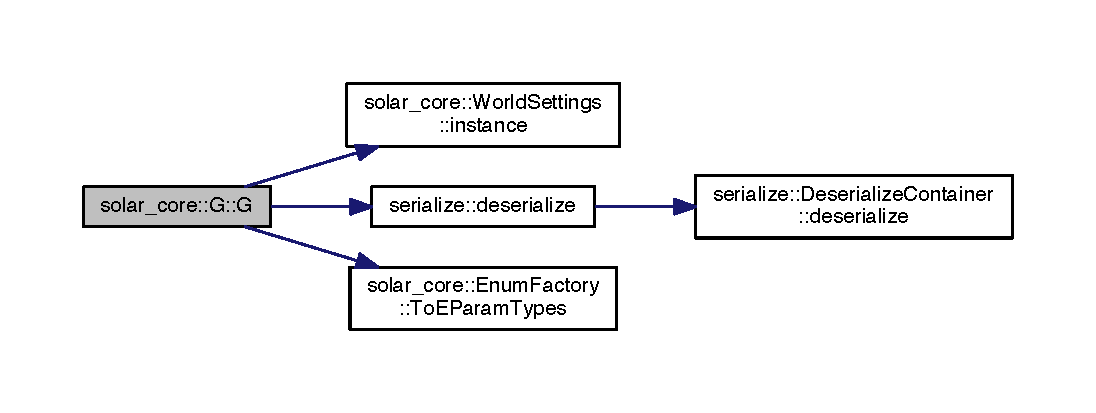
\includegraphics[width=350pt]{classsolar__core_1_1_g_a624adac31ade604e0335717bad4fc9cd_cgraph}
\end{center}
\end{figure}




\subsection{Member Function Documentation}
\hypertarget{classsolar__core_1_1_g_ae01d6ea43c397cc79356884c98caf277}{}\index{solar\+\_\+core\+::\+G@{solar\+\_\+core\+::\+G}!ac\+\_\+update\+\_\+tick@{ac\+\_\+update\+\_\+tick}}
\index{ac\+\_\+update\+\_\+tick@{ac\+\_\+update\+\_\+tick}!solar\+\_\+core\+::\+G@{solar\+\_\+core\+::\+G}}
\subsubsection[{ac\+\_\+update\+\_\+tick}]{\setlength{\rightskip}{0pt plus 5cm}void G\+::ac\+\_\+update\+\_\+tick (
\begin{DoxyParamCaption}
{}
\end{DoxyParamCaption}
)\hspace{0.3cm}{\ttfamily [protected]}}\label{classsolar__core_1_1_g_ae01d6ea43c397cc79356884c98caf277}
Parameters of government 

Definition at line 103 of file G.\+cpp.



Here is the call graph for this function\+:\nopagebreak
\begin{figure}[H]
\begin{center}
\leavevmode
\includegraphics[width=350pt]{classsolar__core_1_1_g_ae01d6ea43c397cc79356884c98caf277_cgraph}
\end{center}
\end{figure}




Here is the caller graph for this function\+:\nopagebreak
\begin{figure}[H]
\begin{center}
\leavevmode
\includegraphics[width=350pt]{classsolar__core_1_1_g_ae01d6ea43c397cc79356884c98caf277_icgraph}
\end{center}
\end{figure}


\hypertarget{classsolar__core_1_1_g_ad3c9fb1da4db51b296c29a6b94b0f139}{}\index{solar\+\_\+core\+::\+G@{solar\+\_\+core\+::\+G}!act\+\_\+tick@{act\+\_\+tick}}
\index{act\+\_\+tick@{act\+\_\+tick}!solar\+\_\+core\+::\+G@{solar\+\_\+core\+::\+G}}
\subsubsection[{act\+\_\+tick}]{\setlength{\rightskip}{0pt plus 5cm}void G\+::act\+\_\+tick (
\begin{DoxyParamCaption}
{}
\end{DoxyParamCaption}
)\hspace{0.3cm}{\ttfamily [virtual]}}\label{classsolar__core_1_1_g_ad3c9fb1da4db51b296c29a6b94b0f139}


Definition at line 146 of file G.\+cpp.



Here is the call graph for this function\+:\nopagebreak
\begin{figure}[H]
\begin{center}
\leavevmode
\includegraphics[width=350pt]{classsolar__core_1_1_g_ad3c9fb1da4db51b296c29a6b94b0f139_cgraph}
\end{center}
\end{figure}




Here is the caller graph for this function\+:\nopagebreak
\begin{figure}[H]
\begin{center}
\leavevmode
\includegraphics[width=346pt]{classsolar__core_1_1_g_ad3c9fb1da4db51b296c29a6b94b0f139_icgraph}
\end{center}
\end{figure}


\hypertarget{classsolar__core_1_1_g_af7498122edc4bfda69724fbd1d59c53d}{}\index{solar\+\_\+core\+::\+G@{solar\+\_\+core\+::\+G}!approve\+\_\+permit@{approve\+\_\+permit}}
\index{approve\+\_\+permit@{approve\+\_\+permit}!solar\+\_\+core\+::\+G@{solar\+\_\+core\+::\+G}}
\subsubsection[{approve\+\_\+permit}]{\setlength{\rightskip}{0pt plus 5cm}void G\+::approve\+\_\+permit (
\begin{DoxyParamCaption}
\item[{std\+::shared\+\_\+ptr$<$ {\bf P\+V\+Project} $>$}]{project\+\_\+}
\end{DoxyParamCaption}
)\hspace{0.3cm}{\ttfamily [protected]}}\label{classsolar__core_1_1_g_af7498122edc4bfda69724fbd1d59c53d}


Definition at line 96 of file G.\+cpp.



Here is the caller graph for this function\+:\nopagebreak
\begin{figure}[H]
\begin{center}
\leavevmode
\includegraphics[width=350pt]{classsolar__core_1_1_g_af7498122edc4bfda69724fbd1d59c53d_icgraph}
\end{center}
\end{figure}


\hypertarget{classsolar__core_1_1_g_aecc948919b4cadba36d15b458eb0b7c3}{}\index{solar\+\_\+core\+::\+G@{solar\+\_\+core\+::\+G}!collect\+\_\+inf\+\_\+site\+\_\+visit@{collect\+\_\+inf\+\_\+site\+\_\+visit}}
\index{collect\+\_\+inf\+\_\+site\+\_\+visit@{collect\+\_\+inf\+\_\+site\+\_\+visit}!solar\+\_\+core\+::\+G@{solar\+\_\+core\+::\+G}}
\subsubsection[{collect\+\_\+inf\+\_\+site\+\_\+visit}]{\setlength{\rightskip}{0pt plus 5cm}void G\+::collect\+\_\+inf\+\_\+site\+\_\+visit (
\begin{DoxyParamCaption}
\item[{std\+::shared\+\_\+ptr$<$ {\bf P\+V\+Project} $>$}]{project\+\_\+}
\end{DoxyParamCaption}
)\hspace{0.3cm}{\ttfamily [protected]}}\label{classsolar__core_1_1_g_aecc948919b4cadba36d15b458eb0b7c3}


Definition at line 77 of file G.\+cpp.



Here is the caller graph for this function\+:\nopagebreak
\begin{figure}[H]
\begin{center}
\leavevmode
\includegraphics[width=350pt]{classsolar__core_1_1_g_aecc948919b4cadba36d15b458eb0b7c3_icgraph}
\end{center}
\end{figure}


\hypertarget{classsolar__core_1_1_g_a0734da633e88ea0f6ff782d4b6521c09}{}\index{solar\+\_\+core\+::\+G@{solar\+\_\+core\+::\+G}!init@{init}}
\index{init@{init}!solar\+\_\+core\+::\+G@{solar\+\_\+core\+::\+G}}
\subsubsection[{init}]{\setlength{\rightskip}{0pt plus 5cm}void G\+::init (
\begin{DoxyParamCaption}
\item[{{\bf W} $\ast$}]{w\+\_\+}
\end{DoxyParamCaption}
)}\label{classsolar__core_1_1_g_a0734da633e88ea0f6ff782d4b6521c09}


Definition at line 56 of file G.\+cpp.



Here is the caller graph for this function\+:\nopagebreak
\begin{figure}[H]
\begin{center}
\leavevmode
\includegraphics[width=310pt]{classsolar__core_1_1_g_a0734da633e88ea0f6ff782d4b6521c09_icgraph}
\end{center}
\end{figure}


\hypertarget{classsolar__core_1_1_g_ae5836aff26a74e47cd26081fb94641bb}{}\index{solar\+\_\+core\+::\+G@{solar\+\_\+core\+::\+G}!request\+\_\+inspection@{request\+\_\+inspection}}
\index{request\+\_\+inspection@{request\+\_\+inspection}!solar\+\_\+core\+::\+G@{solar\+\_\+core\+::\+G}}
\subsubsection[{request\+\_\+inspection}]{\setlength{\rightskip}{0pt plus 5cm}void G\+::request\+\_\+inspection (
\begin{DoxyParamCaption}
\item[{std\+::shared\+\_\+ptr$<$ {\bf P\+V\+Project} $>$}]{project\+\_\+}
\end{DoxyParamCaption}
)}\label{classsolar__core_1_1_g_ae5836aff26a74e47cd26081fb94641bb}
request inspection after installation 

Definition at line 83 of file G.\+cpp.



Here is the caller graph for this function\+:\nopagebreak
\begin{figure}[H]
\begin{center}
\leavevmode
\includegraphics[width=350pt]{classsolar__core_1_1_g_ae5836aff26a74e47cd26081fb94641bb_icgraph}
\end{center}
\end{figure}


\hypertarget{classsolar__core_1_1_g_a615600f35d73a38ea48e99909fff5085}{}\index{solar\+\_\+core\+::\+G@{solar\+\_\+core\+::\+G}!request\+\_\+permit\+\_\+for\+\_\+installation@{request\+\_\+permit\+\_\+for\+\_\+installation}}
\index{request\+\_\+permit\+\_\+for\+\_\+installation@{request\+\_\+permit\+\_\+for\+\_\+installation}!solar\+\_\+core\+::\+G@{solar\+\_\+core\+::\+G}}
\subsubsection[{request\+\_\+permit\+\_\+for\+\_\+installation}]{\setlength{\rightskip}{0pt plus 5cm}void G\+::request\+\_\+permit\+\_\+for\+\_\+installation (
\begin{DoxyParamCaption}
\item[{std\+::shared\+\_\+ptr$<$ {\bf P\+V\+Project} $>$}]{project\+\_\+}
\end{DoxyParamCaption}
)\hspace{0.3cm}{\ttfamily [virtual]}}\label{classsolar__core_1_1_g_a615600f35d73a38ea48e99909fff5085}
Section relevant for permitting processrequest permit for the project 

Definition at line 66 of file G.\+cpp.



Here is the caller graph for this function\+:\nopagebreak
\begin{figure}[H]
\begin{center}
\leavevmode
\includegraphics[width=350pt]{classsolar__core_1_1_g_a615600f35d73a38ea48e99909fff5085_icgraph}
\end{center}
\end{figure}




\subsection{Member Data Documentation}
\hypertarget{classsolar__core_1_1_g_a4d5b2845fc790c0f14b13fe922821f4b}{}\index{solar\+\_\+core\+::\+G@{solar\+\_\+core\+::\+G}!a\+\_\+time@{a\+\_\+time}}
\index{a\+\_\+time@{a\+\_\+time}!solar\+\_\+core\+::\+G@{solar\+\_\+core\+::\+G}}
\subsubsection[{a\+\_\+time}]{\setlength{\rightskip}{0pt plus 5cm}{\bf Time\+Unit} solar\+\_\+core\+::\+G\+::a\+\_\+time\hspace{0.3cm}{\ttfamily [protected]}}\label{classsolar__core_1_1_g_a4d5b2845fc790c0f14b13fe922821f4b}


Definition at line 116 of file G.\+h.

\hypertarget{classsolar__core_1_1_g_a5c79440fcadc7d3e9212c5e7c05f84f7}{}\index{solar\+\_\+core\+::\+G@{solar\+\_\+core\+::\+G}!i\+\_\+schedule\+\_\+visits@{i\+\_\+schedule\+\_\+visits}}
\index{i\+\_\+schedule\+\_\+visits@{i\+\_\+schedule\+\_\+visits}!solar\+\_\+core\+::\+G@{solar\+\_\+core\+::\+G}}
\subsubsection[{i\+\_\+schedule\+\_\+visits}]{\setlength{\rightskip}{0pt plus 5cm}std\+::size\+\_\+t solar\+\_\+core\+::\+G\+::i\+\_\+schedule\+\_\+visits\hspace{0.3cm}{\ttfamily [protected]}}\label{classsolar__core_1_1_g_a5c79440fcadc7d3e9212c5e7c05f84f7}


Definition at line 88 of file G.\+h.

\hypertarget{classsolar__core_1_1_g_a045f1db40b15301ed5ec8aefb5327b0e}{}\index{solar\+\_\+core\+::\+G@{solar\+\_\+core\+::\+G}!params@{params}}
\index{params@{params}!solar\+\_\+core\+::\+G@{solar\+\_\+core\+::\+G}}
\subsubsection[{params}]{\setlength{\rightskip}{0pt plus 5cm}std\+::map$<${\bf E\+Param\+Types}, double$>$ solar\+\_\+core\+::\+G\+::params\hspace{0.3cm}{\ttfamily [protected]}}\label{classsolar__core_1_1_g_a045f1db40b15301ed5ec8aefb5327b0e}
Section with internal parameters 

Definition at line 109 of file G.\+h.

\hypertarget{classsolar__core_1_1_g_a3a87f9e5c14cd5bae4be8a4da538181e}{}\index{solar\+\_\+core\+::\+G@{solar\+\_\+core\+::\+G}!pending\+\_\+pvprojects@{pending\+\_\+pvprojects}}
\index{pending\+\_\+pvprojects@{pending\+\_\+pvprojects}!solar\+\_\+core\+::\+G@{solar\+\_\+core\+::\+G}}
\subsubsection[{pending\+\_\+pvprojects}]{\setlength{\rightskip}{0pt plus 5cm}std\+::deque$<$std\+::shared\+\_\+ptr$<${\bf P\+V\+Project}$>$ $>$ solar\+\_\+core\+::\+G\+::pending\+\_\+pvprojects\hspace{0.3cm}{\ttfamily [protected]}}\label{classsolar__core_1_1_g_a3a87f9e5c14cd5bae4be8a4da538181e}
Section relevant for permitting process 

Definition at line 82 of file G.\+h.

\hypertarget{classsolar__core_1_1_g_a7ae124e062dbd50b0da66f34c9633965}{}\index{solar\+\_\+core\+::\+G@{solar\+\_\+core\+::\+G}!pending\+\_\+pvprojects\+\_\+lock@{pending\+\_\+pvprojects\+\_\+lock}}
\index{pending\+\_\+pvprojects\+\_\+lock@{pending\+\_\+pvprojects\+\_\+lock}!solar\+\_\+core\+::\+G@{solar\+\_\+core\+::\+G}}
\subsubsection[{pending\+\_\+pvprojects\+\_\+lock}]{\setlength{\rightskip}{0pt plus 5cm}std\+::mutex solar\+\_\+core\+::\+G\+::pending\+\_\+pvprojects\+\_\+lock\hspace{0.3cm}{\ttfamily [protected]}}\label{classsolar__core_1_1_g_a7ae124e062dbd50b0da66f34c9633965}


Definition at line 84 of file G.\+h.

\hypertarget{classsolar__core_1_1_g_a053a3d2c00c5af66925ebe359c4b4228}{}\index{solar\+\_\+core\+::\+G@{solar\+\_\+core\+::\+G}!pending\+\_\+pvprojects\+\_\+to\+\_\+add@{pending\+\_\+pvprojects\+\_\+to\+\_\+add}}
\index{pending\+\_\+pvprojects\+\_\+to\+\_\+add@{pending\+\_\+pvprojects\+\_\+to\+\_\+add}!solar\+\_\+core\+::\+G@{solar\+\_\+core\+::\+G}}
\subsubsection[{pending\+\_\+pvprojects\+\_\+to\+\_\+add}]{\setlength{\rightskip}{0pt plus 5cm}std\+::deque$<$std\+::shared\+\_\+ptr$<${\bf P\+V\+Project}$>$ $>$ solar\+\_\+core\+::\+G\+::pending\+\_\+pvprojects\+\_\+to\+\_\+add\hspace{0.3cm}{\ttfamily [protected]}}\label{classsolar__core_1_1_g_a053a3d2c00c5af66925ebe359c4b4228}


Definition at line 83 of file G.\+h.

\hypertarget{classsolar__core_1_1_g_a26b220870264c1927d282dfe9412725e}{}\index{solar\+\_\+core\+::\+G@{solar\+\_\+core\+::\+G}!project\+\_\+states\+\_\+to\+\_\+delete@{project\+\_\+states\+\_\+to\+\_\+delete}}
\index{project\+\_\+states\+\_\+to\+\_\+delete@{project\+\_\+states\+\_\+to\+\_\+delete}!solar\+\_\+core\+::\+G@{solar\+\_\+core\+::\+G}}
\subsubsection[{project\+\_\+states\+\_\+to\+\_\+delete}]{\setlength{\rightskip}{0pt plus 5cm}std\+::set$<${\bf E\+Param\+Types}$>$ solar\+\_\+core\+::\+G\+::project\+\_\+states\+\_\+to\+\_\+delete\hspace{0.3cm}{\ttfamily [protected]}}\label{classsolar__core_1_1_g_a26b220870264c1927d282dfe9412725e}


Definition at line 95 of file G.\+h.

\hypertarget{classsolar__core_1_1_g_a33472d3b331a303ec8a9b61e2da163d3}{}\index{solar\+\_\+core\+::\+G@{solar\+\_\+core\+::\+G}!schedule\+\_\+visits@{schedule\+\_\+visits}}
\index{schedule\+\_\+visits@{schedule\+\_\+visits}!solar\+\_\+core\+::\+G@{solar\+\_\+core\+::\+G}}
\subsubsection[{schedule\+\_\+visits}]{\setlength{\rightskip}{0pt plus 5cm}std\+::vector$<$std\+::vector$<$std\+::weak\+\_\+ptr$<${\bf P\+V\+Project}$>$ $>$ $>$ solar\+\_\+core\+::\+G\+::schedule\+\_\+visits\hspace{0.3cm}{\ttfamily [protected]}}\label{classsolar__core_1_1_g_a33472d3b331a303ec8a9b61e2da163d3}
schedule for visits for the permitting accessment, length is equal to the Max\+Length\+Wait\+Permit\+Visit.\begin{DoxyRefDesc}{Dev\+Stage2}
\item[\hyperlink{_dev_stage2__DevStage2000002}{Dev\+Stage2}]think about it, not every jurisdiction will need it \end{DoxyRefDesc}


Definition at line 86 of file G.\+h.

\hypertarget{classsolar__core_1_1_g_a7239d05d617261f97c46b641a0229c14}{}\index{solar\+\_\+core\+::\+G@{solar\+\_\+core\+::\+G}!w@{w}}
\index{w@{w}!solar\+\_\+core\+::\+G@{solar\+\_\+core\+::\+G}}
\subsubsection[{w}]{\setlength{\rightskip}{0pt plus 5cm}{\bf W}$\ast$ solar\+\_\+core\+::\+G\+::w\hspace{0.3cm}{\ttfamily [protected]}}\label{classsolar__core_1_1_g_a7239d05d617261f97c46b641a0229c14}


Definition at line 114 of file G.\+h.



The documentation for this class was generated from the following files\+:\begin{DoxyCompactItemize}
\item 
/\+Users/wilfeli/\+Dropbox/\+A\+B\+M/\+Solar\+Panels/\+A\+B\+M\+I\+R\+I\+S\+Lab/\+Source/\+Agents/\hyperlink{_g_8h}{G.\+h}\item 
/\+Users/wilfeli/\+Dropbox/\+A\+B\+M/\+Solar\+Panels/\+A\+B\+M\+I\+R\+I\+S\+Lab/\+Source/\+Agents/\hyperlink{_g_8cpp}{G.\+cpp}\end{DoxyCompactItemize}

\hypertarget{classsolar__core_1_1_helper_w}{}\section{solar\+\_\+core\+:\+:Helper\+W Class Reference}
\label{classsolar__core_1_1_helper_w}\index{solar\+\_\+core\+::\+Helper\+W@{solar\+\_\+core\+::\+Helper\+W}}


{\ttfamily \#include $<$Helper\+W.\+h$>$}



Inheritance diagram for solar\+\_\+core\+:\+:Helper\+W\+:
\nopagebreak
\begin{figure}[H]
\begin{center}
\leavevmode
\includegraphics[width=350pt]{classsolar__core_1_1_helper_w__inherit__graph}
\end{center}
\end{figure}
\subsection*{Public Member Functions}
\begin{DoxyCompactItemize}
\item 
virtual std\+::vector$<$ \hyperlink{classsolar__core_1_1_s_e_i}{S\+E\+I} $\ast$ $>$ \hyperlink{classsolar__core_1_1_helper_w_a2d53e9a0f5945ced5ddc0388278d2336}{create\+\_\+seis} (\hyperlink{namespacesolar__core_adeda2737d6938c190eb774a5b2495045}{Property\+Tree} \&pt\+\_\+, std\+::string mode\+\_\+, long N\+\_\+\+S\+E\+I, long N\+\_\+\+S\+E\+I\+Large, boost\+::variate\+\_\+generator$<$ boost\+::mt19937 \&, boost\+::uniform\+\_\+int$<$ uint64\+\_\+t $>$$>$ \&rng\+\_\+location\+\_\+x, boost\+::variate\+\_\+generator$<$ boost\+::mt19937 \&, boost\+::uniform\+\_\+int$<$ uint64\+\_\+t $>$$>$ \&rng\+\_\+location\+\_\+y, \hyperlink{classsolar__core_1_1_w}{W} $\ast$w\+\_\+)=0
\end{DoxyCompactItemize}


\subsection{Detailed Description}


Definition at line 24 of file Helper\+W.\+h.



\subsection{Member Function Documentation}
\hypertarget{classsolar__core_1_1_helper_w_a2d53e9a0f5945ced5ddc0388278d2336}{}\index{solar\+\_\+core\+::\+Helper\+W@{solar\+\_\+core\+::\+Helper\+W}!create\+\_\+seis@{create\+\_\+seis}}
\index{create\+\_\+seis@{create\+\_\+seis}!solar\+\_\+core\+::\+Helper\+W@{solar\+\_\+core\+::\+Helper\+W}}
\subsubsection[{create\+\_\+seis}]{\setlength{\rightskip}{0pt plus 5cm}virtual std\+::vector$<${\bf S\+E\+I}$\ast$$>$ solar\+\_\+core\+::\+Helper\+W\+::create\+\_\+seis (
\begin{DoxyParamCaption}
\item[{{\bf Property\+Tree} \&}]{pt\+\_\+, }
\item[{std\+::string}]{mode\+\_\+, }
\item[{long}]{N\+\_\+\+S\+E\+I, }
\item[{long}]{N\+\_\+\+S\+E\+I\+Large, }
\item[{boost\+::variate\+\_\+generator$<$ boost\+::mt19937 \&, boost\+::uniform\+\_\+int$<$ uint64\+\_\+t $>$$>$ \&}]{rng\+\_\+location\+\_\+x, }
\item[{boost\+::variate\+\_\+generator$<$ boost\+::mt19937 \&, boost\+::uniform\+\_\+int$<$ uint64\+\_\+t $>$$>$ \&}]{rng\+\_\+location\+\_\+y, }
\item[{{\bf W} $\ast$}]{w\+\_\+}
\end{DoxyParamCaption}
)\hspace{0.3cm}{\ttfamily [pure virtual]}}\label{classsolar__core_1_1_helper_w_a2d53e9a0f5945ced5ddc0388278d2336}


Implemented in \hyperlink{classsolar__core_1_1_helper_w_specialization_3_01_t_00_01_unit_test_model_01_4_adf23c2c9808e7d9ef18a4d778bacccce}{solar\+\_\+core\+::\+Helper\+W\+Specialization$<$ T, Unit\+Test\+Model $>$}, \hyperlink{classsolar__core_1_1_helper_w_specialization_3_01_t_00_01_baseline_model_01_4_a9f9f25055cdc6e402ae717b540a1feac}{solar\+\_\+core\+::\+Helper\+W\+Specialization$<$ T, Baseline\+Model $>$}, and \hyperlink{classsolar__core_1_1_helper_w_specialization_a738f047f9e421dcac3739f9898242c09}{solar\+\_\+core\+::\+Helper\+W\+Specialization$<$ T, Param $>$}.



Here is the caller graph for this function\+:
\nopagebreak
\begin{figure}[H]
\begin{center}
\leavevmode
\includegraphics[width=318pt]{classsolar__core_1_1_helper_w_a2d53e9a0f5945ced5ddc0388278d2336_icgraph}
\end{center}
\end{figure}




The documentation for this class was generated from the following file\+:\begin{DoxyCompactItemize}
\item 
/\+Users/wilfeli/\+Dropbox/\+A\+B\+M/\+Solar\+Panels/\+A\+B\+M\+I\+R\+I\+S\+Lab/\+Source/\+U\+I/\hyperlink{_helper_w_8h}{Helper\+W.\+h}\end{DoxyCompactItemize}

\hypertarget{classsolar__core_1_1_helper_w_specialization}{}\section{solar\+\_\+core\+:\+:Helper\+W\+Specialization$<$ T, Param $>$ Class Template Reference}
\label{classsolar__core_1_1_helper_w_specialization}\index{solar\+\_\+core\+::\+Helper\+W\+Specialization$<$ T, Param $>$@{solar\+\_\+core\+::\+Helper\+W\+Specialization$<$ T, Param $>$}}


{\ttfamily \#include $<$Helper\+W.\+h$>$}



Inheritance diagram for solar\+\_\+core\+:\+:Helper\+W\+Specialization$<$ T, Param $>$\+:
\nopagebreak
\begin{figure}[H]
\begin{center}
\leavevmode
\includegraphics[width=248pt]{classsolar__core_1_1_helper_w_specialization__inherit__graph}
\end{center}
\end{figure}


Collaboration diagram for solar\+\_\+core\+:\+:Helper\+W\+Specialization$<$ T, Param $>$\+:
\nopagebreak
\begin{figure}[H]
\begin{center}
\leavevmode
\includegraphics[width=248pt]{classsolar__core_1_1_helper_w_specialization__coll__graph}
\end{center}
\end{figure}
\subsection*{Public Member Functions}
\begin{DoxyCompactItemize}
\item 
std\+::vector$<$ \hyperlink{classsolar__core_1_1_s_e_i}{S\+E\+I} $\ast$ $>$ \hyperlink{classsolar__core_1_1_helper_w_specialization_a738f047f9e421dcac3739f9898242c09}{create\+\_\+seis} (\hyperlink{namespacesolar__core_adeda2737d6938c190eb774a5b2495045}{Property\+Tree} \&pt\+\_\+, std\+::string mode\+\_\+, long N\+\_\+\+S\+E\+I, long N\+\_\+\+S\+E\+I\+Large, boost\+::variate\+\_\+generator$<$ boost\+::mt19937 \&, boost\+::uniform\+\_\+int$<$ uint64\+\_\+t $>$$>$ \&rng\+\_\+location\+\_\+x, boost\+::variate\+\_\+generator$<$ boost\+::mt19937 \&, boost\+::uniform\+\_\+int$<$ uint64\+\_\+t $>$$>$ \&rng\+\_\+location\+\_\+y, \hyperlink{classsolar__core_1_1_w}{W} $\ast$w\+\_\+) override
\end{DoxyCompactItemize}


\subsection{Detailed Description}
\subsubsection*{template$<$class T, class Param$>$class solar\+\_\+core\+::\+Helper\+W\+Specialization$<$ T, Param $>$}



Definition at line 32 of file Helper\+W.\+h.



\subsection{Member Function Documentation}
\hypertarget{classsolar__core_1_1_helper_w_specialization_a738f047f9e421dcac3739f9898242c09}{}\index{solar\+\_\+core\+::\+Helper\+W\+Specialization@{solar\+\_\+core\+::\+Helper\+W\+Specialization}!create\+\_\+seis@{create\+\_\+seis}}
\index{create\+\_\+seis@{create\+\_\+seis}!solar\+\_\+core\+::\+Helper\+W\+Specialization@{solar\+\_\+core\+::\+Helper\+W\+Specialization}}
\subsubsection[{create\+\_\+seis}]{\setlength{\rightskip}{0pt plus 5cm}template$<$class T , class Param $>$ std\+::vector$<${\bf S\+E\+I}$\ast$$>$ {\bf solar\+\_\+core\+::\+Helper\+W\+Specialization}$<$ T, Param $>$\+::create\+\_\+seis (
\begin{DoxyParamCaption}
\item[{{\bf Property\+Tree} \&}]{pt\+\_\+, }
\item[{std\+::string}]{mode\+\_\+, }
\item[{long}]{N\+\_\+\+S\+E\+I, }
\item[{long}]{N\+\_\+\+S\+E\+I\+Large, }
\item[{boost\+::variate\+\_\+generator$<$ boost\+::mt19937 \&, boost\+::uniform\+\_\+int$<$ uint64\+\_\+t $>$$>$ \&}]{rng\+\_\+location\+\_\+x, }
\item[{boost\+::variate\+\_\+generator$<$ boost\+::mt19937 \&, boost\+::uniform\+\_\+int$<$ uint64\+\_\+t $>$$>$ \&}]{rng\+\_\+location\+\_\+y, }
\item[{{\bf W} $\ast$}]{w\+\_\+}
\end{DoxyParamCaption}
)\hspace{0.3cm}{\ttfamily [inline]}, {\ttfamily [override]}, {\ttfamily [virtual]}}\label{classsolar__core_1_1_helper_w_specialization_a738f047f9e421dcac3739f9898242c09}


Implements \hyperlink{classsolar__core_1_1_helper_w_a2d53e9a0f5945ced5ddc0388278d2336}{solar\+\_\+core\+::\+Helper\+W}.



Definition at line 36 of file Helper\+W.\+h.



The documentation for this class was generated from the following file\+:\begin{DoxyCompactItemize}
\item 
/\+Users/wilfeli/\+Dropbox/\+A\+B\+M/\+Solar\+Panels/\+A\+B\+M\+I\+R\+I\+S\+Lab/\+Source/\+U\+I/\hyperlink{_helper_w_8h}{Helper\+W.\+h}\end{DoxyCompactItemize}

\hypertarget{classsolar__core_1_1_helper_w_specialization_3_01_t_00_01_baseline_model_01_4}{}\section{solar\+\_\+core\+:\+:Helper\+W\+Specialization$<$ T, Baseline\+Model $>$ Class Template Reference}
\label{classsolar__core_1_1_helper_w_specialization_3_01_t_00_01_baseline_model_01_4}\index{solar\+\_\+core\+::\+Helper\+W\+Specialization$<$ T, Baseline\+Model $>$@{solar\+\_\+core\+::\+Helper\+W\+Specialization$<$ T, Baseline\+Model $>$}}


{\ttfamily \#include $<$Helper\+W.\+h$>$}



Inheritance diagram for solar\+\_\+core\+:\+:Helper\+W\+Specialization$<$ T, Baseline\+Model $>$\+:\nopagebreak
\begin{figure}[H]
\begin{center}
\leavevmode
\includegraphics[width=248pt]{classsolar__core_1_1_helper_w_specialization_3_01_t_00_01_baseline_model_01_4__inherit__graph}
\end{center}
\end{figure}


Collaboration diagram for solar\+\_\+core\+:\+:Helper\+W\+Specialization$<$ T, Baseline\+Model $>$\+:\nopagebreak
\begin{figure}[H]
\begin{center}
\leavevmode
\includegraphics[width=248pt]{classsolar__core_1_1_helper_w_specialization_3_01_t_00_01_baseline_model_01_4__coll__graph}
\end{center}
\end{figure}
\subsection*{Public Member Functions}
\begin{DoxyCompactItemize}
\item 
std\+::vector$<$ \hyperlink{classsolar__core_1_1_s_e_i}{S\+E\+I} $\ast$ $>$ \hyperlink{classsolar__core_1_1_helper_w_specialization_3_01_t_00_01_baseline_model_01_4_a9f9f25055cdc6e402ae717b540a1feac}{create\+\_\+seis} (\hyperlink{namespacesolar__core_adeda2737d6938c190eb774a5b2495045}{Property\+Tree} \&pt, std\+::string mode\+\_\+, long N\+\_\+\+S\+E\+I, long N\+\_\+\+S\+E\+I\+Large, boost\+::variate\+\_\+generator$<$ boost\+::mt19937 \&, boost\+::uniform\+\_\+int$<$ uint64\+\_\+t $>$$>$ \&rng\+\_\+location\+\_\+x, boost\+::variate\+\_\+generator$<$ boost\+::mt19937 \&, boost\+::uniform\+\_\+int$<$ uint64\+\_\+t $>$$>$ \&rng\+\_\+location\+\_\+y, \hyperlink{classsolar__core_1_1_w}{W} $\ast$w\+\_\+)
\item 
std\+::vector$<$ \hyperlink{classsolar__core_1_1_household}{Household} $\ast$ $>$ \hyperlink{classsolar__core_1_1_helper_w_specialization_3_01_t_00_01_baseline_model_01_4_aaf9f30218e0bc792ed2817caf89b576d}{create\+\_\+hhs} (\hyperlink{namespacesolar__core_adeda2737d6938c190eb774a5b2495045}{Property\+Tree} \&pt, std\+::string mode\+\_\+, long N\+\_\+\+H\+H, long N\+\_\+\+H\+H\+Marketing\+State\+Highly\+Interested, boost\+::variate\+\_\+generator$<$ boost\+::mt19937 \&, boost\+::uniform\+\_\+int$<$ uint64\+\_\+t $>$$>$ \&rng\+\_\+location\+\_\+x, boost\+::variate\+\_\+generator$<$ boost\+::mt19937 \&, boost\+::uniform\+\_\+int$<$ uint64\+\_\+t $>$$>$ \&rng\+\_\+location\+\_\+y, \hyperlink{classsolar__core_1_1_i_random}{I\+Random} $\ast$rand)
\end{DoxyCompactItemize}


\subsection{Detailed Description}
\subsubsection*{template$<$class T$>$class solar\+\_\+core\+::\+Helper\+W\+Specialization$<$ T, Baseline\+Model $>$}



Definition at line 48 of file Helper\+W.\+h.



\subsection{Member Function Documentation}
\hypertarget{classsolar__core_1_1_helper_w_specialization_3_01_t_00_01_baseline_model_01_4_aaf9f30218e0bc792ed2817caf89b576d}{}\index{solar\+\_\+core\+::\+Helper\+W\+Specialization$<$ T, Baseline\+Model $>$@{solar\+\_\+core\+::\+Helper\+W\+Specialization$<$ T, Baseline\+Model $>$}!create\+\_\+hhs@{create\+\_\+hhs}}
\index{create\+\_\+hhs@{create\+\_\+hhs}!solar\+\_\+core\+::\+Helper\+W\+Specialization$<$ T, Baseline\+Model $>$@{solar\+\_\+core\+::\+Helper\+W\+Specialization$<$ T, Baseline\+Model $>$}}
\subsubsection[{create\+\_\+hhs}]{\setlength{\rightskip}{0pt plus 5cm}template$<$class T $>$ std\+::vector$<${\bf Household}$\ast$$>$ {\bf solar\+\_\+core\+::\+Helper\+W\+Specialization}$<$ T, {\bf Baseline\+Model} $>$\+::create\+\_\+hhs (
\begin{DoxyParamCaption}
\item[{{\bf Property\+Tree} \&}]{pt, }
\item[{std\+::string}]{mode\+\_\+, }
\item[{long}]{N\+\_\+\+H\+H, }
\item[{long}]{N\+\_\+\+H\+H\+Marketing\+State\+Highly\+Interested, }
\item[{boost\+::variate\+\_\+generator$<$ boost\+::mt19937 \&, boost\+::uniform\+\_\+int$<$ uint64\+\_\+t $>$$>$ \&}]{rng\+\_\+location\+\_\+x, }
\item[{boost\+::variate\+\_\+generator$<$ boost\+::mt19937 \&, boost\+::uniform\+\_\+int$<$ uint64\+\_\+t $>$$>$ \&}]{rng\+\_\+location\+\_\+y, }
\item[{{\bf I\+Random} $\ast$}]{rand}
\end{DoxyParamCaption}
)\hspace{0.3cm}{\ttfamily [inline]}}\label{classsolar__core_1_1_helper_w_specialization_3_01_t_00_01_baseline_model_01_4_aaf9f30218e0bc792ed2817caf89b576d}
Old version of generating H -\/ with independent parameters 

Definition at line 97 of file Helper\+W.\+h.



Here is the call graph for this function\+:
\nopagebreak
\begin{figure}[H]
\begin{center}
\leavevmode
\includegraphics[width=350pt]{classsolar__core_1_1_helper_w_specialization_3_01_t_00_01_baseline_model_01_4_aaf9f30218e0bc792ed2817caf89b576d_cgraph}
\end{center}
\end{figure}


\hypertarget{classsolar__core_1_1_helper_w_specialization_3_01_t_00_01_baseline_model_01_4_a9f9f25055cdc6e402ae717b540a1feac}{}\index{solar\+\_\+core\+::\+Helper\+W\+Specialization$<$ T, Baseline\+Model $>$@{solar\+\_\+core\+::\+Helper\+W\+Specialization$<$ T, Baseline\+Model $>$}!create\+\_\+seis@{create\+\_\+seis}}
\index{create\+\_\+seis@{create\+\_\+seis}!solar\+\_\+core\+::\+Helper\+W\+Specialization$<$ T, Baseline\+Model $>$@{solar\+\_\+core\+::\+Helper\+W\+Specialization$<$ T, Baseline\+Model $>$}}
\subsubsection[{create\+\_\+seis}]{\setlength{\rightskip}{0pt plus 5cm}template$<$class T $>$ std\+::vector$<${\bf S\+E\+I}$\ast$$>$ {\bf solar\+\_\+core\+::\+Helper\+W\+Specialization}$<$ T, {\bf Baseline\+Model} $>$\+::create\+\_\+seis (
\begin{DoxyParamCaption}
\item[{{\bf Property\+Tree} \&}]{pt, }
\item[{std\+::string}]{mode\+\_\+, }
\item[{long}]{N\+\_\+\+S\+E\+I, }
\item[{long}]{N\+\_\+\+S\+E\+I\+Large, }
\item[{boost\+::variate\+\_\+generator$<$ boost\+::mt19937 \&, boost\+::uniform\+\_\+int$<$ uint64\+\_\+t $>$$>$ \&}]{rng\+\_\+location\+\_\+x, }
\item[{boost\+::variate\+\_\+generator$<$ boost\+::mt19937 \&, boost\+::uniform\+\_\+int$<$ uint64\+\_\+t $>$$>$ \&}]{rng\+\_\+location\+\_\+y, }
\item[{{\bf W} $\ast$}]{w\+\_\+}
\end{DoxyParamCaption}
)\hspace{0.3cm}{\ttfamily [inline]}, {\ttfamily [virtual]}}\label{classsolar__core_1_1_helper_w_specialization_3_01_t_00_01_baseline_model_01_4_a9f9f25055cdc6e402ae717b540a1feac}


Implements \hyperlink{classsolar__core_1_1_helper_w_a2d53e9a0f5945ced5ddc0388278d2336}{solar\+\_\+core\+::\+Helper\+W}.



Definition at line 52 of file Helper\+W.\+h.



Here is the call graph for this function\+:\nopagebreak
\begin{figure}[H]
\begin{center}
\leavevmode
\includegraphics[width=350pt]{classsolar__core_1_1_helper_w_specialization_3_01_t_00_01_baseline_model_01_4_a9f9f25055cdc6e402ae717b540a1feac_cgraph}
\end{center}
\end{figure}




The documentation for this class was generated from the following file\+:\begin{DoxyCompactItemize}
\item 
/\+Users/wilfeli/\+Dropbox/\+A\+B\+M/\+Solar\+Panels/\+A\+B\+M\+I\+R\+I\+S\+Lab/\+Source/\+U\+I/\hyperlink{_helper_w_8h}{Helper\+W.\+h}\end{DoxyCompactItemize}

\hypertarget{classsolar__core_1_1_helper_w_specialization_3_01_t_00_01_unit_test_model_01_4}{}\section{solar\+\_\+core\+:\+:Helper\+W\+Specialization$<$ T, Unit\+Test\+Model $>$ Class Template Reference}
\label{classsolar__core_1_1_helper_w_specialization_3_01_t_00_01_unit_test_model_01_4}\index{solar\+\_\+core\+::\+Helper\+W\+Specialization$<$ T, Unit\+Test\+Model $>$@{solar\+\_\+core\+::\+Helper\+W\+Specialization$<$ T, Unit\+Test\+Model $>$}}


{\ttfamily \#include $<$Helper\+W.\+h$>$}



Inheritance diagram for solar\+\_\+core\+:\+:Helper\+W\+Specialization$<$ T, Unit\+Test\+Model $>$\+:\nopagebreak
\begin{figure}[H]
\begin{center}
\leavevmode
\includegraphics[width=248pt]{classsolar__core_1_1_helper_w_specialization_3_01_t_00_01_unit_test_model_01_4__inherit__graph}
\end{center}
\end{figure}


Collaboration diagram for solar\+\_\+core\+:\+:Helper\+W\+Specialization$<$ T, Unit\+Test\+Model $>$\+:\nopagebreak
\begin{figure}[H]
\begin{center}
\leavevmode
\includegraphics[width=248pt]{classsolar__core_1_1_helper_w_specialization_3_01_t_00_01_unit_test_model_01_4__coll__graph}
\end{center}
\end{figure}
\subsection*{Public Member Functions}
\begin{DoxyCompactItemize}
\item 
std\+::vector$<$ \hyperlink{classsolar__core_1_1_s_e_i}{S\+E\+I} $\ast$ $>$ \hyperlink{classsolar__core_1_1_helper_w_specialization_3_01_t_00_01_unit_test_model_01_4_adf23c2c9808e7d9ef18a4d778bacccce}{create\+\_\+seis} (\hyperlink{namespacesolar__core_adeda2737d6938c190eb774a5b2495045}{Property\+Tree} \&pt, std\+::string mode\+\_\+, long N\+\_\+\+S\+E\+I, long N\+\_\+\+S\+E\+I\+Large, boost\+::variate\+\_\+generator$<$ boost\+::mt19937 \&, boost\+::uniform\+\_\+int$<$ uint64\+\_\+t $>$$>$ \&rng\+\_\+location\+\_\+x, boost\+::variate\+\_\+generator$<$ boost\+::mt19937 \&, boost\+::uniform\+\_\+int$<$ uint64\+\_\+t $>$$>$ \&rng\+\_\+location\+\_\+y, \hyperlink{classsolar__core_1_1_w}{W} $\ast$w\+\_\+)
\end{DoxyCompactItemize}


\subsection{Detailed Description}
\subsubsection*{template$<$class T$>$class solar\+\_\+core\+::\+Helper\+W\+Specialization$<$ T, Unit\+Test\+Model $>$}



Definition at line 207 of file Helper\+W.\+h.



\subsection{Member Function Documentation}
\hypertarget{classsolar__core_1_1_helper_w_specialization_3_01_t_00_01_unit_test_model_01_4_adf23c2c9808e7d9ef18a4d778bacccce}{}\index{solar\+\_\+core\+::\+Helper\+W\+Specialization$<$ T, Unit\+Test\+Model $>$@{solar\+\_\+core\+::\+Helper\+W\+Specialization$<$ T, Unit\+Test\+Model $>$}!create\+\_\+seis@{create\+\_\+seis}}
\index{create\+\_\+seis@{create\+\_\+seis}!solar\+\_\+core\+::\+Helper\+W\+Specialization$<$ T, Unit\+Test\+Model $>$@{solar\+\_\+core\+::\+Helper\+W\+Specialization$<$ T, Unit\+Test\+Model $>$}}
\subsubsection[{create\+\_\+seis}]{\setlength{\rightskip}{0pt plus 5cm}template$<$class T $>$ std\+::vector$<${\bf S\+E\+I}$\ast$$>$ {\bf solar\+\_\+core\+::\+Helper\+W\+Specialization}$<$ T, {\bf Unit\+Test\+Model} $>$\+::create\+\_\+seis (
\begin{DoxyParamCaption}
\item[{{\bf Property\+Tree} \&}]{pt, }
\item[{std\+::string}]{mode\+\_\+, }
\item[{long}]{N\+\_\+\+S\+E\+I, }
\item[{long}]{N\+\_\+\+S\+E\+I\+Large, }
\item[{boost\+::variate\+\_\+generator$<$ boost\+::mt19937 \&, boost\+::uniform\+\_\+int$<$ uint64\+\_\+t $>$$>$ \&}]{rng\+\_\+location\+\_\+x, }
\item[{boost\+::variate\+\_\+generator$<$ boost\+::mt19937 \&, boost\+::uniform\+\_\+int$<$ uint64\+\_\+t $>$$>$ \&}]{rng\+\_\+location\+\_\+y, }
\item[{{\bf W} $\ast$}]{w\+\_\+}
\end{DoxyParamCaption}
)\hspace{0.3cm}{\ttfamily [inline]}, {\ttfamily [virtual]}}\label{classsolar__core_1_1_helper_w_specialization_3_01_t_00_01_unit_test_model_01_4_adf23c2c9808e7d9ef18a4d778bacccce}


Implements \hyperlink{classsolar__core_1_1_helper_w_a2d53e9a0f5945ced5ddc0388278d2336}{solar\+\_\+core\+::\+Helper\+W}.



Definition at line 211 of file Helper\+W.\+h.



Here is the call graph for this function\+:\nopagebreak
\begin{figure}[H]
\begin{center}
\leavevmode
\includegraphics[width=350pt]{classsolar__core_1_1_helper_w_specialization_3_01_t_00_01_unit_test_model_01_4_adf23c2c9808e7d9ef18a4d778bacccce_cgraph}
\end{center}
\end{figure}




The documentation for this class was generated from the following file\+:\begin{DoxyCompactItemize}
\item 
/\+Users/wilfeli/\+Dropbox/\+A\+B\+M/\+Solar\+Panels/\+A\+B\+M\+I\+R\+I\+S\+Lab/\+Source/\+U\+I/\hyperlink{_helper_w_8h}{Helper\+W.\+h}\end{DoxyCompactItemize}

\hypertarget{classsolar__core_1_1_house}{}\section{solar\+\_\+core\+:\+:House Class Reference}
\label{classsolar__core_1_1_house}\index{solar\+\_\+core\+::\+House@{solar\+\_\+core\+::\+House}}


{\ttfamily \#include $<$Geography.\+h$>$}



Collaboration diagram for solar\+\_\+core\+:\+:House\+:\nopagebreak
\begin{figure}[H]
\begin{center}
\leavevmode
\includegraphics[width=178pt]{classsolar__core_1_1_house__coll__graph}
\end{center}
\end{figure}
\subsection*{Public Member Functions}
\begin{DoxyCompactItemize}
\item 
\hyperlink{classsolar__core_1_1_house_a1babbd79506a4acf93c16ceec093b924}{House} (const \hyperlink{namespacesolar__core_adeda2737d6938c190eb774a5b2495045}{Property\+Tree} \&pt\+\_\+)
\end{DoxyCompactItemize}
\subsection*{Public Attributes}
\begin{DoxyCompactItemize}
\item 
double \hyperlink{classsolar__core_1_1_house_aa6491ce4f3fc6d99a59ea80cfb8194fc}{roof\+\_\+age}
\item 
double \hyperlink{classsolar__core_1_1_house_a7f872cb768b83e70e263590078fa4c7d}{roof\+\_\+size}
\end{DoxyCompactItemize}


\subsection{Detailed Description}
Belongs to a \hyperlink{classsolar__core_1_1_household}{Household}.

Cuurently switched to estimated roof\+\_\+size from the house\+\_\+size
\begin{DoxyEnumerate}
\item R\+P = roof pitch
\item H\+S = square foot of home
\item F = number of floors
\item x = roof pitched length
\item y = roof length
\item R\+A = roof area
\item R = ratio of roof area to house area
\end{DoxyEnumerate}

Formula for calculating roof size \[ y = \sqrt{frac{HS}{F}} \] \[ x = (\frac{y}{2}) \times (\cos (\arctan (RP)) \] \[ RA = 2 \times x \times y \] \[ R = RA \div HS \] 

Definition at line 51 of file Geography.\+h.



\subsection{Constructor \& Destructor Documentation}
\hypertarget{classsolar__core_1_1_house_a1babbd79506a4acf93c16ceec093b924}{}\index{solar\+\_\+core\+::\+House@{solar\+\_\+core\+::\+House}!House@{House}}
\index{House@{House}!solar\+\_\+core\+::\+House@{solar\+\_\+core\+::\+House}}
\subsubsection[{House}]{\setlength{\rightskip}{0pt plus 5cm}House\+::\+House (
\begin{DoxyParamCaption}
\item[{const {\bf Property\+Tree} \&}]{pt\+\_\+}
\end{DoxyParamCaption}
)}\label{classsolar__core_1_1_house_a1babbd79506a4acf93c16ceec093b924}


Definition at line 16 of file Geography.\+cpp.



\subsection{Member Data Documentation}
\hypertarget{classsolar__core_1_1_house_aa6491ce4f3fc6d99a59ea80cfb8194fc}{}\index{solar\+\_\+core\+::\+House@{solar\+\_\+core\+::\+House}!roof\+\_\+age@{roof\+\_\+age}}
\index{roof\+\_\+age@{roof\+\_\+age}!solar\+\_\+core\+::\+House@{solar\+\_\+core\+::\+House}}
\subsubsection[{roof\+\_\+age}]{\setlength{\rightskip}{0pt plus 5cm}double solar\+\_\+core\+::\+House\+::roof\+\_\+age}\label{classsolar__core_1_1_house_aa6491ce4f3fc6d99a59ea80cfb8194fc}
age of a house\textquotesingle{}s roof in years (not required to be whole years) 

Definition at line 55 of file Geography.\+h.

\hypertarget{classsolar__core_1_1_house_a7f872cb768b83e70e263590078fa4c7d}{}\index{solar\+\_\+core\+::\+House@{solar\+\_\+core\+::\+House}!roof\+\_\+size@{roof\+\_\+size}}
\index{roof\+\_\+size@{roof\+\_\+size}!solar\+\_\+core\+::\+House@{solar\+\_\+core\+::\+House}}
\subsubsection[{roof\+\_\+size}]{\setlength{\rightskip}{0pt plus 5cm}double solar\+\_\+core\+::\+House\+::roof\+\_\+size}\label{classsolar__core_1_1_house_a7f872cb768b83e70e263590078fa4c7d}
size of a roof, in m$^\wedge$2 

Definition at line 56 of file Geography.\+h.



The documentation for this class was generated from the following files\+:\begin{DoxyCompactItemize}
\item 
/\+Users/wilfeli/\+Dropbox/\+A\+B\+M/\+Solar\+Panels/\+A\+B\+M\+I\+R\+I\+S\+Lab/\+Source/\+Geography/\hyperlink{_geography_8h}{Geography.\+h}\item 
/\+Users/wilfeli/\+Dropbox/\+A\+B\+M/\+Solar\+Panels/\+A\+B\+M\+I\+R\+I\+S\+Lab/\+Source/\+Geography/\hyperlink{_geography_8cpp}{Geography.\+cpp}\end{DoxyCompactItemize}

\hypertarget{classsolar__core_1_1_household}{}\section{solar\+\_\+core\+:\+:Household Class Reference}
\label{classsolar__core_1_1_household}\index{solar\+\_\+core\+::\+Household@{solar\+\_\+core\+::\+Household}}


{\ttfamily \#include $<$H.\+h$>$}



Inheritance diagram for solar\+\_\+core\+:\+:Household\+:\nopagebreak
\begin{figure}[H]
\begin{center}
\leavevmode
\includegraphics[width=196pt]{classsolar__core_1_1_household__inherit__graph}
\end{center}
\end{figure}


Collaboration diagram for solar\+\_\+core\+:\+:Household\+:
\nopagebreak
\begin{figure}[H]
\begin{center}
\leavevmode
\includegraphics[width=350pt]{classsolar__core_1_1_household__coll__graph}
\end{center}
\end{figure}
\subsection*{Public Member Functions}
{\bf }\par
\begin{DoxyCompactItemize}
\item 
virtual void \hyperlink{classsolar__core_1_1_household_a165b7c64c72e5ed4ea08307e32082517}{ac\+\_\+inf\+\_\+quoting\+\_\+sei} ()
\item 
virtual void \hyperlink{classsolar__core_1_1_household_a1e7d20a60dc42b8d09a8d23a4cdb26a6}{act\+\_\+tick} ()
\end{DoxyCompactItemize}

{\bf }\par
\begin{DoxyCompactItemize}
\item 
virtual void \hyperlink{classsolar__core_1_1_household_ac9d26af7b52f0cdc357fc5dca4b86ad9}{get\+\_\+inf} (std\+::shared\+\_\+ptr$<$ \hyperlink{classsolar__core_1_1_mes_marketing_s_e_i}{Mes\+Marketing\+S\+E\+I} $>$ mes\+\_\+) override
\end{DoxyCompactItemize}

{\bf }\par
\begin{DoxyCompactItemize}
\item 
virtual std\+::shared\+\_\+ptr$<$ \hyperlink{classsolar__core_1_1_mes_state_base_h_h}{Mes\+State\+Base\+H\+H} $>$ \hyperlink{classsolar__core_1_1_household_a008a18ff8c2d15da72e19876dc896a4e}{get\+\_\+inf\+\_\+online\+\_\+quote} (\hyperlink{classsolar__core_1_1_i_agent}{I\+Agent} $\ast$agent\+\_\+to)
\item 
virtual void \hyperlink{classsolar__core_1_1_household_a31a1c8d006fb9e95a2460aa392eaa830}{receive\+\_\+preliminary\+\_\+quote} (std\+::shared\+\_\+ptr$<$ \hyperlink{classsolar__core_1_1_p_v_project}{P\+V\+Project} $>$ project\+\_\+)
\item 
virtual void \hyperlink{classsolar__core_1_1_household_a306aed410a39e8062ab5f1b4a3216b8b}{receive\+\_\+online\+\_\+quote} (std\+::shared\+\_\+ptr$<$ \hyperlink{classsolar__core_1_1_p_v_project}{P\+V\+Project} $>$ project\+\_\+)
\item 
virtual bool \hyperlink{classsolar__core_1_1_household_a8c9635bac11c9bd93e65dbb5be5b9d85}{request\+\_\+time\+\_\+slot\+\_\+visit} (\hyperlink{namespacesolar__core_a4b5949d07259da6f8a20d12a30403e90}{Time\+Unit} visit\+\_\+time, std\+::weak\+\_\+ptr$<$ \hyperlink{classsolar__core_1_1_p_v_project}{P\+V\+Project} $>$ project)
\item 
virtual bool \hyperlink{classsolar__core_1_1_household_a8d4b9c4a5cf59c93f33489eccbfba7db}{schedule\+\_\+visit} (\hyperlink{namespacesolar__core_a4b5949d07259da6f8a20d12a30403e90}{Time\+Unit} visit\+\_\+time, std\+::weak\+\_\+ptr$<$ \hyperlink{classsolar__core_1_1_p_v_project}{P\+V\+Project} $>$ project)
\item 
virtual bool \hyperlink{classsolar__core_1_1_household_aa63241ca3fcc1f2374d10b5c7f44124a}{dec\+\_\+project\+\_\+reroof} (std\+::shared\+\_\+ptr$<$ \hyperlink{classsolar__core_1_1_p_v_project}{P\+V\+Project} $>$ project)
\end{DoxyCompactItemize}

{\bf }\par
\begin{DoxyCompactItemize}
\item 
virtual void \hyperlink{classsolar__core_1_1_household_a7df346780d3d9683293af565d5831d05}{receive\+\_\+design} (std\+::shared\+\_\+ptr$<$ \hyperlink{classsolar__core_1_1_p_v_project}{P\+V\+Project} $>$ project\+\_\+)
\end{DoxyCompactItemize}

\subsection*{Public Attributes}
{\bf }\par
\begin{DoxyCompactItemize}
\item 
double \hyperlink{classsolar__core_1_1_household_a6596375631a366fdd24270f75548841f}{location\+\_\+x}
\item 
double \hyperlink{classsolar__core_1_1_household_a1ba6b7af82982096e05d99a70a2647eb}{location\+\_\+y}
\end{DoxyCompactItemize}

{\bf }\par
\begin{DoxyCompactItemize}
\item 
\hyperlink{classsolar__core_1_1_house}{House} $\ast$ \hyperlink{classsolar__core_1_1_household_a1104d8264fe733937e1fd2e9ad0f8fc1}{house}
\end{DoxyCompactItemize}

\subsection*{Protected Attributes}
{\bf }\par
\begin{DoxyCompactItemize}
\item 
std\+::map$<$ \hyperlink{namespacesolar__core_aa1147341e5ef7a40d68d1bd68e149362}{E\+Param\+Types}, double $>$ \hyperlink{classsolar__core_1_1_household_a41d61dc3bab971cb19170341b77d9df8}{params}
\end{DoxyCompactItemize}

{\bf }\par
\begin{DoxyCompactItemize}
\item 
std\+::vector$<$ std\+::shared\+\_\+ptr$<$ \hyperlink{classsolar__core_1_1_p_v_project}{P\+V\+Project} $>$ $>$ \hyperlink{classsolar__core_1_1_household_a79c0e955af98669487e0fb472811f842}{pvprojects}
\end{DoxyCompactItemize}

{\bf }\par
\begin{DoxyCompactItemize}
\item 
std\+::deque$<$ std\+::shared\+\_\+ptr$<$ \hyperlink{classsolar__core_1_1_mes_marketing_s_e_i}{Mes\+Marketing\+S\+E\+I} $>$ $>$ \hyperlink{classsolar__core_1_1_household_a3ae4cec5fca43ee5ca3287a01f5a05a2}{get\+\_\+inf\+\_\+marketing\+\_\+sei}
\item 
std\+::deque$<$ std\+::shared\+\_\+ptr$<$ \hyperlink{classsolar__core_1_1_mes_marketing_s_e_i_preliminary_quote}{Mes\+Marketing\+S\+E\+I\+Preliminary\+Quote} $>$ $>$ \hyperlink{classsolar__core_1_1_household_a297842358a2d79db160566106972bc0d}{preliminary\+\_\+quotes}
\item 
\hyperlink{namespacesolar__core_aa1147341e5ef7a40d68d1bd68e149362}{E\+Param\+Types} \hyperlink{classsolar__core_1_1_household_a3ee8b2654cad46236d11f85a4ccd9574}{marketing\+\_\+state}
\end{DoxyCompactItemize}

{\bf }\par
\begin{DoxyCompactItemize}
\item 
\hyperlink{namespacesolar__core_aa1147341e5ef7a40d68d1bd68e149362}{E\+Param\+Types} \hyperlink{classsolar__core_1_1_household_a4ae618de9a28895317824b185b57ab24}{quote\+\_\+state}
\item 
std\+::vector$<$ std\+::vector$<$ std\+::weak\+\_\+ptr$<$ \hyperlink{classsolar__core_1_1_p_v_project}{P\+V\+Project} $>$ $>$ $>$ \hyperlink{classsolar__core_1_1_household_aadd4e3e2fc66ed214bcfadf37f557b14}{schedule\+\_\+visits}
\item 
std\+::size\+\_\+t \hyperlink{classsolar__core_1_1_household_a077c668f06c009a43c535f1ad92cf92e}{i\+\_\+schedule\+\_\+visits}
\item 
std\+::mutex \hyperlink{classsolar__core_1_1_household_a15e598cfc419040a23f75fe08a8ef1d8}{schedule\+\_\+visits\+\_\+lock}
\item 
long \hyperlink{classsolar__core_1_1_household_a6b35426fd691daa6d352ec34a6ec6e4d}{quote\+\_\+stage\+\_\+timer}
\item 
long \hyperlink{classsolar__core_1_1_household_aedfc08b7837a3e2fa6ad9e62309694f3}{n\+\_\+preliminary\+\_\+quotes}
\end{DoxyCompactItemize}

{\bf }\par
\begin{DoxyCompactItemize}
\item 
std\+::deque$<$ std\+::shared\+\_\+ptr$<$ \hyperlink{classsolar__core_1_1_p_v_project}{P\+V\+Project} $>$ $>$ \hyperlink{classsolar__core_1_1_household_ad4409e81251bdd33d9dca1cd1225dc75}{accepted\+\_\+design}
\item 
long \hyperlink{classsolar__core_1_1_household_ac82a6ebca38ecaf971845f6fa5791559}{n\+\_\+pending\+\_\+designs}
\end{DoxyCompactItemize}

{\bf }\par
\begin{DoxyCompactItemize}
\item 
\hyperlink{classsolar__core_1_1_w}{W} $\ast$ \hyperlink{classsolar__core_1_1_household_a01ac4643c725f397ba7485209a906e4d}{w}
\end{DoxyCompactItemize}

\begin{DoxyCompactItemize}
\item 
\hyperlink{namespacesolar__core_a4b5949d07259da6f8a20d12a30403e90}{Time\+Unit} \hyperlink{classsolar__core_1_1_household_ad323100235079f34537ccda656e86e64}{a\+\_\+time}
\item 
virtual void \hyperlink{classsolar__core_1_1_household_a2d8c80f6db68610fb3e0f9b48e1e490b}{dec\+\_\+evaluate\+\_\+online\+\_\+quotes} ()
\item 
virtual void \hyperlink{classsolar__core_1_1_household_a6e27e36f623bd307eedcd97c550d5c5e}{dec\+\_\+evaluate\+\_\+preliminary\+\_\+quotes} ()
\item 
virtual void \hyperlink{classsolar__core_1_1_household_a733a90456d57f698b3aa974c6c6e0108}{update\+\_\+params} ()
\item 
virtual void \hyperlink{classsolar__core_1_1_household_ac73de13d0d4b4e01b2defbb85872c4b2}{ac\+\_\+update\+\_\+tick} ()
\end{DoxyCompactItemize}


\subsection{Detailed Description}
Has multiple humans, but they are not modelled as decision agents only the H\+H is the decision making agent.

\begin{DoxyRefDesc}{Solar W\+P}
\item[\hyperlink{wp__wp000001}{Solar W\+P}]Once survey is completed will have data\+: what are your choices and decisions on solar panels. The same logic as in \hyperlink{classsolar__core_1_1_s_e_i}{S\+E\+I}. Hidden parameter/factor is utility of accepting project. Might be more complex to estimate as will have a lot of categorical data.\end{DoxyRefDesc}


\begin{DoxyRefDesc}{Dev\+Stage3}
\item[\hyperlink{_dev_stage3__DevStage3000002}{Dev\+Stage3}]think about using \href{http://en.cppreference.com/w/cpp/types/result_of}{\tt http\+://en.\+cppreference.\+com/w/cpp/types/result\+\_\+of} -\/ very neat construction\end{DoxyRefDesc}


\begin{DoxyRefDesc}{Dev\+Stage2}
\item[\hyperlink{_dev_stage2__DevStage2000004}{Dev\+Stage2}]might change from actually assigning house to assigning house type (memory considerations)\end{DoxyRefDesc}


Definition at line 47 of file H.\+h.



\subsection{Member Function Documentation}
\hypertarget{classsolar__core_1_1_household_a165b7c64c72e5ed4ea08307e32082517}{}\index{solar\+\_\+core\+::\+Household@{solar\+\_\+core\+::\+Household}!ac\+\_\+inf\+\_\+quoting\+\_\+sei@{ac\+\_\+inf\+\_\+quoting\+\_\+sei}}
\index{ac\+\_\+inf\+\_\+quoting\+\_\+sei@{ac\+\_\+inf\+\_\+quoting\+\_\+sei}!solar\+\_\+core\+::\+Household@{solar\+\_\+core\+::\+Household}}
\subsubsection[{ac\+\_\+inf\+\_\+quoting\+\_\+sei}]{\setlength{\rightskip}{0pt plus 5cm}void Household\+::ac\+\_\+inf\+\_\+quoting\+\_\+sei (
\begin{DoxyParamCaption}
{}
\end{DoxyParamCaption}
)\hspace{0.3cm}{\ttfamily [virtual]}}\label{classsolar__core_1_1_household_a165b7c64c72e5ed4ea08307e32082517}
Creation and initialization section

\begin{DoxyRefDesc}{Dev\+Stage2}
\item[\hyperlink{_dev_stage2__DevStage2000005}{Dev\+Stage2}]need destructor, copy constructor, copy assignment operator, move constructor, move assignment operator\end{DoxyRefDesc}


C(const C\&) = default; // Copy constructor C(\+C\&\&) = default; // Move constructor C\& operator=(const C\&) \& = default; // Copy assignment operator C\& operator=(\+C\&\&) \& = default; // Move assignment operator virtual $\sim$\+C() \{ \} // Destructor

see \href{http://stackoverflow.com/questions/4782757/rule-of-three-becomes-rule-of-five-with-c11}{\tt http\+://stackoverflow.\+com/questions/4782757/rule-\/of-\/three-\/becomes-\/rule-\/of-\/five-\/with-\/c11}

Section with actions in the worldaction to request information from \hyperlink{classsolar__core_1_1_s_e_i}{S\+E\+I} when initiative is given from the \hyperlink{classsolar__core_1_1_w}{W} \begin{DoxyRefDesc}{Dev\+Stage2}
\item[\hyperlink{_dev_stage2__DevStage2000002}{Dev\+Stage2}]think about moving difference to the virtual call. For now it is explicit, as it is assumed that agents themselves realize that it will be online vs offline quote \end{DoxyRefDesc}


Definition at line 40 of file H.\+cpp.



Here is the call graph for this function\+:
\nopagebreak
\begin{figure}[H]
\begin{center}
\leavevmode
\includegraphics[width=350pt]{classsolar__core_1_1_household_a165b7c64c72e5ed4ea08307e32082517_cgraph}
\end{center}
\end{figure}




Here is the caller graph for this function\+:
\nopagebreak
\begin{figure}[H]
\begin{center}
\leavevmode
\includegraphics[width=350pt]{classsolar__core_1_1_household_a165b7c64c72e5ed4ea08307e32082517_icgraph}
\end{center}
\end{figure}


\hypertarget{classsolar__core_1_1_household_ac73de13d0d4b4e01b2defbb85872c4b2}{}\index{solar\+\_\+core\+::\+Household@{solar\+\_\+core\+::\+Household}!ac\+\_\+update\+\_\+tick@{ac\+\_\+update\+\_\+tick}}
\index{ac\+\_\+update\+\_\+tick@{ac\+\_\+update\+\_\+tick}!solar\+\_\+core\+::\+Household@{solar\+\_\+core\+::\+Household}}
\subsubsection[{ac\+\_\+update\+\_\+tick}]{\setlength{\rightskip}{0pt plus 5cm}void Household\+::ac\+\_\+update\+\_\+tick (
\begin{DoxyParamCaption}
{}
\end{DoxyParamCaption}
)\hspace{0.3cm}{\ttfamily [protected]}, {\ttfamily [virtual]}}\label{classsolar__core_1_1_household_ac73de13d0d4b4e01b2defbb85872c4b2}
update internals for the tick 

Definition at line 265 of file H.\+cpp.



Here is the call graph for this function\+:
\nopagebreak
\begin{figure}[H]
\begin{center}
\leavevmode
\includegraphics[width=350pt]{classsolar__core_1_1_household_ac73de13d0d4b4e01b2defbb85872c4b2_cgraph}
\end{center}
\end{figure}




Here is the caller graph for this function\+:
\nopagebreak
\begin{figure}[H]
\begin{center}
\leavevmode
\includegraphics[width=350pt]{classsolar__core_1_1_household_ac73de13d0d4b4e01b2defbb85872c4b2_icgraph}
\end{center}
\end{figure}


\hypertarget{classsolar__core_1_1_household_a1e7d20a60dc42b8d09a8d23a4cdb26a6}{}\index{solar\+\_\+core\+::\+Household@{solar\+\_\+core\+::\+Household}!act\+\_\+tick@{act\+\_\+tick}}
\index{act\+\_\+tick@{act\+\_\+tick}!solar\+\_\+core\+::\+Household@{solar\+\_\+core\+::\+Household}}
\subsubsection[{act\+\_\+tick}]{\setlength{\rightskip}{0pt plus 5cm}void Household\+::act\+\_\+tick (
\begin{DoxyParamCaption}
{}
\end{DoxyParamCaption}
)\hspace{0.3cm}{\ttfamily [virtual]}}\label{classsolar__core_1_1_household_a1e7d20a60dc42b8d09a8d23a4cdb26a6}
generic actions on a tick, specialize for each type of agents generally actions in a tick depend on the state of an agent, either it is choosing installer or waiting for the project to finish. Might have a call back to w that will indicate that this agent has changed state. In this case w will have multiple lists of agents in different states and would call appropriate function. Or might do it internally where new state will dictate behavior in the tick. Generally have both -\/ agent is broadcasting changed state and behaves differently depending on the state. 

Implements \hyperlink{classsolar__core_1_1_i_agent_a6813e8e4f94ab2dc917a29c4d6609149}{solar\+\_\+core\+::\+I\+Agent}.



Definition at line 291 of file H.\+cpp.



Here is the call graph for this function\+:
\nopagebreak
\begin{figure}[H]
\begin{center}
\leavevmode
\includegraphics[width=350pt]{classsolar__core_1_1_household_a1e7d20a60dc42b8d09a8d23a4cdb26a6_cgraph}
\end{center}
\end{figure}


\hypertarget{classsolar__core_1_1_household_a2d8c80f6db68610fb3e0f9b48e1e490b}{}\index{solar\+\_\+core\+::\+Household@{solar\+\_\+core\+::\+Household}!dec\+\_\+evaluate\+\_\+online\+\_\+quotes@{dec\+\_\+evaluate\+\_\+online\+\_\+quotes}}
\index{dec\+\_\+evaluate\+\_\+online\+\_\+quotes@{dec\+\_\+evaluate\+\_\+online\+\_\+quotes}!solar\+\_\+core\+::\+Household@{solar\+\_\+core\+::\+Household}}
\subsubsection[{dec\+\_\+evaluate\+\_\+online\+\_\+quotes}]{\setlength{\rightskip}{0pt plus 5cm}void Household\+::dec\+\_\+evaluate\+\_\+online\+\_\+quotes (
\begin{DoxyParamCaption}
{}
\end{DoxyParamCaption}
)\hspace{0.3cm}{\ttfamily [protected]}, {\ttfamily [virtual]}}\label{classsolar__core_1_1_household_a2d8c80f6db68610fb3e0f9b48e1e490b}
Section with agent\textquotesingle{}s internalseveluate online quotes -\/ which to be persued further 

Definition at line 100 of file H.\+cpp.



Here is the call graph for this function\+:
\nopagebreak
\begin{figure}[H]
\begin{center}
\leavevmode
\includegraphics[width=350pt]{classsolar__core_1_1_household_a2d8c80f6db68610fb3e0f9b48e1e490b_cgraph}
\end{center}
\end{figure}




Here is the caller graph for this function\+:
\nopagebreak
\begin{figure}[H]
\begin{center}
\leavevmode
\includegraphics[width=350pt]{classsolar__core_1_1_household_a2d8c80f6db68610fb3e0f9b48e1e490b_icgraph}
\end{center}
\end{figure}


\hypertarget{classsolar__core_1_1_household_a6e27e36f623bd307eedcd97c550d5c5e}{}\index{solar\+\_\+core\+::\+Household@{solar\+\_\+core\+::\+Household}!dec\+\_\+evaluate\+\_\+preliminary\+\_\+quotes@{dec\+\_\+evaluate\+\_\+preliminary\+\_\+quotes}}
\index{dec\+\_\+evaluate\+\_\+preliminary\+\_\+quotes@{dec\+\_\+evaluate\+\_\+preliminary\+\_\+quotes}!solar\+\_\+core\+::\+Household@{solar\+\_\+core\+::\+Household}}
\subsubsection[{dec\+\_\+evaluate\+\_\+preliminary\+\_\+quotes}]{\setlength{\rightskip}{0pt plus 5cm}void Household\+::dec\+\_\+evaluate\+\_\+preliminary\+\_\+quotes (
\begin{DoxyParamCaption}
{}
\end{DoxyParamCaption}
)\hspace{0.3cm}{\ttfamily [protected]}, {\ttfamily [virtual]}}\label{classsolar__core_1_1_household_a6e27e36f623bd307eedcd97c550d5c5e}
eveluate preliminary quotes -\/ which to be persued further  G\+U\+I\+D research. Boost G\+U\+I\+D is almost unique, uses machine and time, so could be repeated if used across machines or time is changed 

Definition at line 131 of file H.\+cpp.



Here is the caller graph for this function\+:
\nopagebreak
\begin{figure}[H]
\begin{center}
\leavevmode
\includegraphics[width=350pt]{classsolar__core_1_1_household_a6e27e36f623bd307eedcd97c550d5c5e_icgraph}
\end{center}
\end{figure}


\hypertarget{classsolar__core_1_1_household_aa63241ca3fcc1f2374d10b5c7f44124a}{}\index{solar\+\_\+core\+::\+Household@{solar\+\_\+core\+::\+Household}!dec\+\_\+project\+\_\+reroof@{dec\+\_\+project\+\_\+reroof}}
\index{dec\+\_\+project\+\_\+reroof@{dec\+\_\+project\+\_\+reroof}!solar\+\_\+core\+::\+Household@{solar\+\_\+core\+::\+Household}}
\subsubsection[{dec\+\_\+project\+\_\+reroof}]{\setlength{\rightskip}{0pt plus 5cm}bool Household\+::dec\+\_\+project\+\_\+reroof (
\begin{DoxyParamCaption}
\item[{std\+::shared\+\_\+ptr$<$ {\bf P\+V\+Project} $>$}]{project}
\end{DoxyParamCaption}
)\hspace{0.3cm}{\ttfamily [virtual]}}\label{classsolar__core_1_1_household_aa63241ca3fcc1f2374d10b5c7f44124a}
\begin{DoxyRefDesc}{Solar W\+P}
\item[\hyperlink{wp__wp000002}{Solar W\+P}]need to ask H\+H how they decide to reroof \end{DoxyRefDesc}


Definition at line 256 of file H.\+cpp.

\hypertarget{classsolar__core_1_1_household_ac9d26af7b52f0cdc357fc5dca4b86ad9}{}\index{solar\+\_\+core\+::\+Household@{solar\+\_\+core\+::\+Household}!get\+\_\+inf@{get\+\_\+inf}}
\index{get\+\_\+inf@{get\+\_\+inf}!solar\+\_\+core\+::\+Household@{solar\+\_\+core\+::\+Household}}
\subsubsection[{get\+\_\+inf}]{\setlength{\rightskip}{0pt plus 5cm}void Household\+::get\+\_\+inf (
\begin{DoxyParamCaption}
\item[{std\+::shared\+\_\+ptr$<$ {\bf Mes\+Marketing\+S\+E\+I} $>$}]{mes\+\_\+}
\end{DoxyParamCaption}
)\hspace{0.3cm}{\ttfamily [override]}, {\ttfamily [virtual]}}\label{classsolar__core_1_1_household_ac9d26af7b52f0cdc357fc5dca4b86ad9}
Section relevant to marketing informationreceives marketing information No mutex guards as only other operation is poping from the front, which does not invalidate anything

\begin{DoxyRefDesc}{Dev\+Stage2}
\item[\hyperlink{_dev_stage2__DevStage2000001}{Dev\+Stage2}]might be addd saving of the time of the marketing message, in this case it will be saved in the form of transformed marketing messages because original message will time stamped at the moment of creation (almost at the beginning of the simulation) \end{DoxyRefDesc}


\begin{DoxyRefDesc}{Dev\+Stage3}
\item[\hyperlink{_dev_stage3__DevStage3000001}{Dev\+Stage3}]check if this agent is interested in the marketing message \end{DoxyRefDesc}


Implements \hyperlink{classsolar__core_1_1_i_agent_aa9ebc762ed032f7084063199747decb6}{solar\+\_\+core\+::\+I\+Agent}.



Definition at line 19 of file H.\+cpp.

\hypertarget{classsolar__core_1_1_household_a008a18ff8c2d15da72e19876dc896a4e}{}\index{solar\+\_\+core\+::\+Household@{solar\+\_\+core\+::\+Household}!get\+\_\+inf\+\_\+online\+\_\+quote@{get\+\_\+inf\+\_\+online\+\_\+quote}}
\index{get\+\_\+inf\+\_\+online\+\_\+quote@{get\+\_\+inf\+\_\+online\+\_\+quote}!solar\+\_\+core\+::\+Household@{solar\+\_\+core\+::\+Household}}
\subsubsection[{get\+\_\+inf\+\_\+online\+\_\+quote}]{\setlength{\rightskip}{0pt plus 5cm}std\+::shared\+\_\+ptr$<$ {\bf Mes\+State\+Base\+H\+H} $>$ Household\+::get\+\_\+inf\+\_\+online\+\_\+quote (
\begin{DoxyParamCaption}
\item[{{\bf I\+Agent} $\ast$}]{agent\+\_\+to}
\end{DoxyParamCaption}
)\hspace{0.3cm}{\ttfamily [virtual]}}\label{classsolar__core_1_1_household_a008a18ff8c2d15da72e19876dc896a4e}
Section relevant to quoting stagefirst request for information from \hyperlink{classsolar__core_1_1_s_e_i}{S\+E\+I}, provides basic information such as credit score and etc. Some parameters need to be taken from \hyperlink{classsolar__core_1_1_house}{House} directly, they are pushed to the general container when changed 

Definition at line 215 of file H.\+cpp.



Here is the call graph for this function\+:\nopagebreak
\begin{figure}[H]
\begin{center}
\leavevmode
\includegraphics[width=350pt]{classsolar__core_1_1_household_a008a18ff8c2d15da72e19876dc896a4e_cgraph}
\end{center}
\end{figure}


\hypertarget{classsolar__core_1_1_household_a7df346780d3d9683293af565d5831d05}{}\index{solar\+\_\+core\+::\+Household@{solar\+\_\+core\+::\+Household}!receive\+\_\+design@{receive\+\_\+design}}
\index{receive\+\_\+design@{receive\+\_\+design}!solar\+\_\+core\+::\+Household@{solar\+\_\+core\+::\+Household}}
\subsubsection[{receive\+\_\+design}]{\setlength{\rightskip}{0pt plus 5cm}void Household\+::receive\+\_\+design (
\begin{DoxyParamCaption}
\item[{std\+::shared\+\_\+ptr$<$ {\bf P\+V\+Project} $>$}]{project\+\_\+}
\end{DoxyParamCaption}
)\hspace{0.3cm}{\ttfamily [virtual]}}\label{classsolar__core_1_1_household_a7df346780d3d9683293af565d5831d05}
Section relevant to design phaseis informed that design is received 

Definition at line 195 of file H.\+cpp.

\hypertarget{classsolar__core_1_1_household_a306aed410a39e8062ab5f1b4a3216b8b}{}\index{solar\+\_\+core\+::\+Household@{solar\+\_\+core\+::\+Household}!receive\+\_\+online\+\_\+quote@{receive\+\_\+online\+\_\+quote}}
\index{receive\+\_\+online\+\_\+quote@{receive\+\_\+online\+\_\+quote}!solar\+\_\+core\+::\+Household@{solar\+\_\+core\+::\+Household}}
\subsubsection[{receive\+\_\+online\+\_\+quote}]{\setlength{\rightskip}{0pt plus 5cm}void Household\+::receive\+\_\+online\+\_\+quote (
\begin{DoxyParamCaption}
\item[{std\+::shared\+\_\+ptr$<$ {\bf P\+V\+Project} $>$}]{project\+\_\+}
\end{DoxyParamCaption}
)\hspace{0.3cm}{\ttfamily [virtual]}}\label{classsolar__core_1_1_household_a306aed410a39e8062ab5f1b4a3216b8b}
empty for now as information is added directly to the project itself 

Definition at line 208 of file H.\+cpp.

\hypertarget{classsolar__core_1_1_household_a31a1c8d006fb9e95a2460aa392eaa830}{}\index{solar\+\_\+core\+::\+Household@{solar\+\_\+core\+::\+Household}!receive\+\_\+preliminary\+\_\+quote@{receive\+\_\+preliminary\+\_\+quote}}
\index{receive\+\_\+preliminary\+\_\+quote@{receive\+\_\+preliminary\+\_\+quote}!solar\+\_\+core\+::\+Household@{solar\+\_\+core\+::\+Household}}
\subsubsection[{receive\+\_\+preliminary\+\_\+quote}]{\setlength{\rightskip}{0pt plus 5cm}void Household\+::receive\+\_\+preliminary\+\_\+quote (
\begin{DoxyParamCaption}
\item[{std\+::shared\+\_\+ptr$<$ {\bf P\+V\+Project} $>$}]{project\+\_\+}
\end{DoxyParamCaption}
)\hspace{0.3cm}{\ttfamily [virtual]}}\label{classsolar__core_1_1_household_a31a1c8d006fb9e95a2460aa392eaa830}
empty for now as information is added directly to the project itself 

Definition at line 202 of file H.\+cpp.

\hypertarget{classsolar__core_1_1_household_a8c9635bac11c9bd93e65dbb5be5b9d85}{}\index{solar\+\_\+core\+::\+Household@{solar\+\_\+core\+::\+Household}!request\+\_\+time\+\_\+slot\+\_\+visit@{request\+\_\+time\+\_\+slot\+\_\+visit}}
\index{request\+\_\+time\+\_\+slot\+\_\+visit@{request\+\_\+time\+\_\+slot\+\_\+visit}!solar\+\_\+core\+::\+Household@{solar\+\_\+core\+::\+Household}}
\subsubsection[{request\+\_\+time\+\_\+slot\+\_\+visit}]{\setlength{\rightskip}{0pt plus 5cm}bool Household\+::request\+\_\+time\+\_\+slot\+\_\+visit (
\begin{DoxyParamCaption}
\item[{{\bf Time\+Unit}}]{visit\+\_\+time, }
\item[{std\+::weak\+\_\+ptr$<$ {\bf P\+V\+Project} $>$}]{project}
\end{DoxyParamCaption}
)\hspace{0.3cm}{\ttfamily [virtual]}}\label{classsolar__core_1_1_household_a8c9635bac11c9bd93e65dbb5be5b9d85}
check that could have a visit at this time 

Definition at line 231 of file H.\+cpp.

\hypertarget{classsolar__core_1_1_household_a8d4b9c4a5cf59c93f33489eccbfba7db}{}\index{solar\+\_\+core\+::\+Household@{solar\+\_\+core\+::\+Household}!schedule\+\_\+visit@{schedule\+\_\+visit}}
\index{schedule\+\_\+visit@{schedule\+\_\+visit}!solar\+\_\+core\+::\+Household@{solar\+\_\+core\+::\+Household}}
\subsubsection[{schedule\+\_\+visit}]{\setlength{\rightskip}{0pt plus 5cm}bool Household\+::schedule\+\_\+visit (
\begin{DoxyParamCaption}
\item[{{\bf Time\+Unit}}]{visit\+\_\+time, }
\item[{std\+::weak\+\_\+ptr$<$ {\bf P\+V\+Project} $>$}]{project}
\end{DoxyParamCaption}
)\hspace{0.3cm}{\ttfamily [virtual]}}\label{classsolar__core_1_1_household_a8d4b9c4a5cf59c93f33489eccbfba7db}
schedules visit at this time, returns false if no slots are open 

Definition at line 238 of file H.\+cpp.

\hypertarget{classsolar__core_1_1_household_a733a90456d57f698b3aa974c6c6e0108}{}\index{solar\+\_\+core\+::\+Household@{solar\+\_\+core\+::\+Household}!update\+\_\+params@{update\+\_\+params}}
\index{update\+\_\+params@{update\+\_\+params}!solar\+\_\+core\+::\+Household@{solar\+\_\+core\+::\+Household}}
\subsubsection[{update\+\_\+params}]{\setlength{\rightskip}{0pt plus 5cm}void Household\+::update\+\_\+params (
\begin{DoxyParamCaption}
{}
\end{DoxyParamCaption}
)\hspace{0.3cm}{\ttfamily [protected]}, {\ttfamily [virtual]}}\label{classsolar__core_1_1_household_a733a90456d57f698b3aa974c6c6e0108}
is called when some part of parameters is updated that is not saved in the main map with parameters. Is used to keep all parameters synchronized. 

Definition at line 341 of file H.\+cpp.



\subsection{Member Data Documentation}
\hypertarget{classsolar__core_1_1_household_ad323100235079f34537ccda656e86e64}{}\index{solar\+\_\+core\+::\+Household@{solar\+\_\+core\+::\+Household}!a\+\_\+time@{a\+\_\+time}}
\index{a\+\_\+time@{a\+\_\+time}!solar\+\_\+core\+::\+Household@{solar\+\_\+core\+::\+Household}}
\subsubsection[{a\+\_\+time}]{\setlength{\rightskip}{0pt plus 5cm}{\bf Time\+Unit} solar\+\_\+core\+::\+Household\+::a\+\_\+time\hspace{0.3cm}{\ttfamily [protected]}}\label{classsolar__core_1_1_household_ad323100235079f34537ccda656e86e64}
internal agent\textquotesingle{}s timer 

Definition at line 279 of file H.\+h.

\hypertarget{classsolar__core_1_1_household_ad4409e81251bdd33d9dca1cd1225dc75}{}\index{solar\+\_\+core\+::\+Household@{solar\+\_\+core\+::\+Household}!accepted\+\_\+design@{accepted\+\_\+design}}
\index{accepted\+\_\+design@{accepted\+\_\+design}!solar\+\_\+core\+::\+Household@{solar\+\_\+core\+::\+Household}}
\subsubsection[{accepted\+\_\+design}]{\setlength{\rightskip}{0pt plus 5cm}std\+::deque$<$std\+::shared\+\_\+ptr$<${\bf P\+V\+Project}$>$ $>$ solar\+\_\+core\+::\+Household\+::accepted\+\_\+design\hspace{0.3cm}{\ttfamily [protected]}}\label{classsolar__core_1_1_household_ad4409e81251bdd33d9dca1cd1225dc75}
Section relevant to design stage 

Definition at line 257 of file H.\+h.

\hypertarget{classsolar__core_1_1_household_a3ae4cec5fca43ee5ca3287a01f5a05a2}{}\index{solar\+\_\+core\+::\+Household@{solar\+\_\+core\+::\+Household}!get\+\_\+inf\+\_\+marketing\+\_\+sei@{get\+\_\+inf\+\_\+marketing\+\_\+sei}}
\index{get\+\_\+inf\+\_\+marketing\+\_\+sei@{get\+\_\+inf\+\_\+marketing\+\_\+sei}!solar\+\_\+core\+::\+Household@{solar\+\_\+core\+::\+Household}}
\subsubsection[{get\+\_\+inf\+\_\+marketing\+\_\+sei}]{\setlength{\rightskip}{0pt plus 5cm}std\+::deque$<$std\+::shared\+\_\+ptr$<${\bf Mes\+Marketing\+S\+E\+I}$>$ $>$ solar\+\_\+core\+::\+Household\+::get\+\_\+inf\+\_\+marketing\+\_\+sei\hspace{0.3cm}{\ttfamily [protected]}}\label{classsolar__core_1_1_household_a3ae4cec5fca43ee5ca3287a01f5a05a2}
Section relevant to marketing informationstores list of marketing infiormation from \hyperlink{classsolar__core_1_1_s_e_i}{S\+E\+I} agents that this agent is interested in geting quotes from 

Definition at line 222 of file H.\+h.

\hypertarget{classsolar__core_1_1_household_a1104d8264fe733937e1fd2e9ad0f8fc1}{}\index{solar\+\_\+core\+::\+Household@{solar\+\_\+core\+::\+Household}!house@{house}}
\index{house@{house}!solar\+\_\+core\+::\+Household@{solar\+\_\+core\+::\+Household}}
\subsubsection[{house}]{\setlength{\rightskip}{0pt plus 5cm}{\bf House}$\ast$ solar\+\_\+core\+::\+Household\+::house}\label{classsolar__core_1_1_household_a1104d8264fe733937e1fd2e9ad0f8fc1}
Location of an agent, y coordinate.\begin{DoxyRefDesc}{Dev\+Stage2}
\item[\hyperlink{_dev_stage2__DevStage2000007}{Dev\+Stage2}]think about decreasing size for this field, use uint64\+\_\+t or smaller for it \end{DoxyRefDesc}


Section with parameters for solar projects, mainly \hyperlink{classsolar__core_1_1_house}{House} for now 

Definition at line 167 of file H.\+h.

\hypertarget{classsolar__core_1_1_household_a077c668f06c009a43c535f1ad92cf92e}{}\index{solar\+\_\+core\+::\+Household@{solar\+\_\+core\+::\+Household}!i\+\_\+schedule\+\_\+visits@{i\+\_\+schedule\+\_\+visits}}
\index{i\+\_\+schedule\+\_\+visits@{i\+\_\+schedule\+\_\+visits}!solar\+\_\+core\+::\+Household@{solar\+\_\+core\+::\+Household}}
\subsubsection[{i\+\_\+schedule\+\_\+visits}]{\setlength{\rightskip}{0pt plus 5cm}std\+::size\+\_\+t solar\+\_\+core\+::\+Household\+::i\+\_\+schedule\+\_\+visits\hspace{0.3cm}{\ttfamily [protected]}}\label{classsolar__core_1_1_household_a077c668f06c009a43c535f1ad92cf92e}


Definition at line 242 of file H.\+h.

\hypertarget{classsolar__core_1_1_household_a6596375631a366fdd24270f75548841f}{}\index{solar\+\_\+core\+::\+Household@{solar\+\_\+core\+::\+Household}!location\+\_\+x@{location\+\_\+x}}
\index{location\+\_\+x@{location\+\_\+x}!solar\+\_\+core\+::\+Household@{solar\+\_\+core\+::\+Household}}
\subsubsection[{location\+\_\+x}]{\setlength{\rightskip}{0pt plus 5cm}double solar\+\_\+core\+::\+Household\+::location\+\_\+x}\label{classsolar__core_1_1_household_a6596375631a366fdd24270f75548841f}
Section with geographical parameters 

Definition at line 150 of file H.\+h.

\hypertarget{classsolar__core_1_1_household_a1ba6b7af82982096e05d99a70a2647eb}{}\index{solar\+\_\+core\+::\+Household@{solar\+\_\+core\+::\+Household}!location\+\_\+y@{location\+\_\+y}}
\index{location\+\_\+y@{location\+\_\+y}!solar\+\_\+core\+::\+Household@{solar\+\_\+core\+::\+Household}}
\subsubsection[{location\+\_\+y}]{\setlength{\rightskip}{0pt plus 5cm}double solar\+\_\+core\+::\+Household\+::location\+\_\+y}\label{classsolar__core_1_1_household_a1ba6b7af82982096e05d99a70a2647eb}
Location of an agent, x coordinate.\begin{DoxyRefDesc}{Dev\+Stage2}
\item[\hyperlink{_dev_stage2__DevStage2000006}{Dev\+Stage2}]think about decreasing size for this field, use uint64\+\_\+t or smaller for it \end{DoxyRefDesc}


Definition at line 151 of file H.\+h.

\hypertarget{classsolar__core_1_1_household_a3ee8b2654cad46236d11f85a4ccd9574}{}\index{solar\+\_\+core\+::\+Household@{solar\+\_\+core\+::\+Household}!marketing\+\_\+state@{marketing\+\_\+state}}
\index{marketing\+\_\+state@{marketing\+\_\+state}!solar\+\_\+core\+::\+Household@{solar\+\_\+core\+::\+Household}}
\subsubsection[{marketing\+\_\+state}]{\setlength{\rightskip}{0pt plus 5cm}{\bf E\+Param\+Types} solar\+\_\+core\+::\+Household\+::marketing\+\_\+state\hspace{0.3cm}{\ttfamily [protected]}}\label{classsolar__core_1_1_household_a3ee8b2654cad46236d11f85a4ccd9574}
could be interested, very interested or not 

Definition at line 226 of file H.\+h.

\hypertarget{classsolar__core_1_1_household_ac82a6ebca38ecaf971845f6fa5791559}{}\index{solar\+\_\+core\+::\+Household@{solar\+\_\+core\+::\+Household}!n\+\_\+pending\+\_\+designs@{n\+\_\+pending\+\_\+designs}}
\index{n\+\_\+pending\+\_\+designs@{n\+\_\+pending\+\_\+designs}!solar\+\_\+core\+::\+Household@{solar\+\_\+core\+::\+Household}}
\subsubsection[{n\+\_\+pending\+\_\+designs}]{\setlength{\rightskip}{0pt plus 5cm}long solar\+\_\+core\+::\+Household\+::n\+\_\+pending\+\_\+designs\hspace{0.3cm}{\ttfamily [protected]}}\label{classsolar__core_1_1_household_ac82a6ebca38ecaf971845f6fa5791559}


Definition at line 258 of file H.\+h.

\hypertarget{classsolar__core_1_1_household_aedfc08b7837a3e2fa6ad9e62309694f3}{}\index{solar\+\_\+core\+::\+Household@{solar\+\_\+core\+::\+Household}!n\+\_\+preliminary\+\_\+quotes@{n\+\_\+preliminary\+\_\+quotes}}
\index{n\+\_\+preliminary\+\_\+quotes@{n\+\_\+preliminary\+\_\+quotes}!solar\+\_\+core\+::\+Household@{solar\+\_\+core\+::\+Household}}
\subsubsection[{n\+\_\+preliminary\+\_\+quotes}]{\setlength{\rightskip}{0pt plus 5cm}long solar\+\_\+core\+::\+Household\+::n\+\_\+preliminary\+\_\+quotes\hspace{0.3cm}{\ttfamily [protected]}}\label{classsolar__core_1_1_household_aedfc08b7837a3e2fa6ad9e62309694f3}
number of preliminary quotes 

Definition at line 246 of file H.\+h.

\hypertarget{classsolar__core_1_1_household_a41d61dc3bab971cb19170341b77d9df8}{}\index{solar\+\_\+core\+::\+Household@{solar\+\_\+core\+::\+Household}!params@{params}}
\index{params@{params}!solar\+\_\+core\+::\+Household@{solar\+\_\+core\+::\+Household}}
\subsubsection[{params}]{\setlength{\rightskip}{0pt plus 5cm}std\+::map$<${\bf E\+Param\+Types}, double$>$ solar\+\_\+core\+::\+Household\+::params\hspace{0.3cm}{\ttfamily [protected]}}\label{classsolar__core_1_1_household_a41d61dc3bab971cb19170341b77d9df8}
Simplification\+: assume only 1 house per hh. If need to increase number of houses, might switch to vector of pointers to houses. Use R\+A\+I\+I here maybe? for managining raw pointer.\begin{DoxyRefDesc}{Dev\+Stage3}
\item[\hyperlink{_dev_stage3__DevStage3000003}{Dev\+Stage3}]think about using smart pointers here, it will simplify management of creation of agents. Cons\+: it will be bigger, management will add time. As house is created once, no need to complicated lifetime management. \end{DoxyRefDesc}


Section with general parameters that describe hh 

Definition at line 187 of file H.\+h.

\hypertarget{classsolar__core_1_1_household_a297842358a2d79db160566106972bc0d}{}\index{solar\+\_\+core\+::\+Household@{solar\+\_\+core\+::\+Household}!preliminary\+\_\+quotes@{preliminary\+\_\+quotes}}
\index{preliminary\+\_\+quotes@{preliminary\+\_\+quotes}!solar\+\_\+core\+::\+Household@{solar\+\_\+core\+::\+Household}}
\subsubsection[{preliminary\+\_\+quotes}]{\setlength{\rightskip}{0pt plus 5cm}std\+::deque$<$std\+::shared\+\_\+ptr$<${\bf Mes\+Marketing\+S\+E\+I\+Preliminary\+Quote}$>$ $>$ solar\+\_\+core\+::\+Household\+::preliminary\+\_\+quotes\hspace{0.3cm}{\ttfamily [protected]}}\label{classsolar__core_1_1_household_a297842358a2d79db160566106972bc0d}
have list of active quotes that need to be acted upon\begin{DoxyRefDesc}{Dev\+Stage2}
\item[\hyperlink{_dev_stage2__DevStage2000008}{Dev\+Stage2}]think about replacing raw pointer with.  choose between week\+\_\+ptr and shared\+\_\+ptr need to think about ownership in time and time of destruction for these messages. \end{DoxyRefDesc}


Definition at line 224 of file H.\+h.

\hypertarget{classsolar__core_1_1_household_a79c0e955af98669487e0fb472811f842}{}\index{solar\+\_\+core\+::\+Household@{solar\+\_\+core\+::\+Household}!pvprojects@{pvprojects}}
\index{pvprojects@{pvprojects}!solar\+\_\+core\+::\+Household@{solar\+\_\+core\+::\+Household}}
\subsubsection[{pvprojects}]{\setlength{\rightskip}{0pt plus 5cm}std\+::vector$<$std\+::shared\+\_\+ptr$<${\bf P\+V\+Project}$>$ $>$ solar\+\_\+core\+::\+Household\+::pvprojects\hspace{0.3cm}{\ttfamily [protected]}}\label{classsolar__core_1_1_household_a79c0e955af98669487e0fb472811f842}
Parameters of a household, such as income, number of humans, etc.

Section with information relevant to potential and active projectslist of active and potential P\+V projects 

Definition at line 200 of file H.\+h.

\hypertarget{classsolar__core_1_1_household_a6b35426fd691daa6d352ec34a6ec6e4d}{}\index{solar\+\_\+core\+::\+Household@{solar\+\_\+core\+::\+Household}!quote\+\_\+stage\+\_\+timer@{quote\+\_\+stage\+\_\+timer}}
\index{quote\+\_\+stage\+\_\+timer@{quote\+\_\+stage\+\_\+timer}!solar\+\_\+core\+::\+Household@{solar\+\_\+core\+::\+Household}}
\subsubsection[{quote\+\_\+stage\+\_\+timer}]{\setlength{\rightskip}{0pt plus 5cm}long solar\+\_\+core\+::\+Household\+::quote\+\_\+stage\+\_\+timer\hspace{0.3cm}{\ttfamily [protected]}}\label{classsolar__core_1_1_household_a6b35426fd691daa6d352ec34a6ec6e4d}
number of ticks spent in a quoting stage 

Definition at line 245 of file H.\+h.

\hypertarget{classsolar__core_1_1_household_a4ae618de9a28895317824b185b57ab24}{}\index{solar\+\_\+core\+::\+Household@{solar\+\_\+core\+::\+Household}!quote\+\_\+state@{quote\+\_\+state}}
\index{quote\+\_\+state@{quote\+\_\+state}!solar\+\_\+core\+::\+Household@{solar\+\_\+core\+::\+Household}}
\subsubsection[{quote\+\_\+state}]{\setlength{\rightskip}{0pt plus 5cm}{\bf E\+Param\+Types} solar\+\_\+core\+::\+Household\+::quote\+\_\+state\hspace{0.3cm}{\ttfamily [protected]}}\label{classsolar__core_1_1_household_a4ae618de9a28895317824b185b57ab24}
Section relevant to quoting stagewill be active quoting or inactive quoting 

Definition at line 238 of file H.\+h.

\hypertarget{classsolar__core_1_1_household_aadd4e3e2fc66ed214bcfadf37f557b14}{}\index{solar\+\_\+core\+::\+Household@{solar\+\_\+core\+::\+Household}!schedule\+\_\+visits@{schedule\+\_\+visits}}
\index{schedule\+\_\+visits@{schedule\+\_\+visits}!solar\+\_\+core\+::\+Household@{solar\+\_\+core\+::\+Household}}
\subsubsection[{schedule\+\_\+visits}]{\setlength{\rightskip}{0pt plus 5cm}std\+::vector$<$std\+::vector$<$std\+::weak\+\_\+ptr$<${\bf P\+V\+Project}$>$ $>$ $>$ solar\+\_\+core\+::\+Household\+::schedule\+\_\+visits\hspace{0.3cm}{\ttfamily [protected]}}\label{classsolar__core_1_1_household_aadd4e3e2fc66ed214bcfadf37f557b14}
schedule for visits for the preliminary quote, length is equal to Max\+Length\+Wait\+Preliminary\+Quote 

Definition at line 241 of file H.\+h.

\hypertarget{classsolar__core_1_1_household_a15e598cfc419040a23f75fe08a8ef1d8}{}\index{solar\+\_\+core\+::\+Household@{solar\+\_\+core\+::\+Household}!schedule\+\_\+visits\+\_\+lock@{schedule\+\_\+visits\+\_\+lock}}
\index{schedule\+\_\+visits\+\_\+lock@{schedule\+\_\+visits\+\_\+lock}!solar\+\_\+core\+::\+Household@{solar\+\_\+core\+::\+Household}}
\subsubsection[{schedule\+\_\+visits\+\_\+lock}]{\setlength{\rightskip}{0pt plus 5cm}std\+::mutex solar\+\_\+core\+::\+Household\+::schedule\+\_\+visits\+\_\+lock\hspace{0.3cm}{\ttfamily [protected]}}\label{classsolar__core_1_1_household_a15e598cfc419040a23f75fe08a8ef1d8}


Definition at line 243 of file H.\+h.

\hypertarget{classsolar__core_1_1_household_a01ac4643c725f397ba7485209a906e4d}{}\index{solar\+\_\+core\+::\+Household@{solar\+\_\+core\+::\+Household}!w@{w}}
\index{w@{w}!solar\+\_\+core\+::\+Household@{solar\+\_\+core\+::\+Household}}
\subsubsection[{w}]{\setlength{\rightskip}{0pt plus 5cm}{\bf W}$\ast$ solar\+\_\+core\+::\+Household\+::w\hspace{0.3cm}{\ttfamily [protected]}}\label{classsolar__core_1_1_household_a01ac4643c725f397ba7485209a906e4d}
Sections with interactions with the worldraw pointer to the actual world 

Definition at line 290 of file H.\+h.



The documentation for this class was generated from the following files\+:\begin{DoxyCompactItemize}
\item 
/\+Users/wilfeli/\+Dropbox/\+A\+B\+M/\+Solar\+Panels/\+A\+B\+M\+I\+R\+I\+S\+Lab/\+Source/\+Agents/\hyperlink{_h_8h}{H.\+h}\item 
/\+Users/wilfeli/\+Dropbox/\+A\+B\+M/\+Solar\+Panels/\+A\+B\+M\+I\+R\+I\+S\+Lab/\+Source/\+Agents/\hyperlink{_h_8cpp}{H.\+cpp}\end{DoxyCompactItemize}

\hypertarget{classsolar__core_1_1_i_agent}{}\section{solar\+\_\+core\+:\+:I\+Agent Class Reference}
\label{classsolar__core_1_1_i_agent}\index{solar\+\_\+core\+::\+I\+Agent@{solar\+\_\+core\+::\+I\+Agent}}


{\ttfamily \#include $<$I\+Agent.\+h$>$}



Inheritance diagram for solar\+\_\+core\+:\+:I\+Agent\+:\nopagebreak
\begin{figure}[H]
\begin{center}
\leavevmode
\includegraphics[width=299pt]{classsolar__core_1_1_i_agent__inherit__graph}
\end{center}
\end{figure}
\subsection*{Public Member Functions}
\begin{DoxyCompactItemize}
\item 
virtual void \hyperlink{classsolar__core_1_1_i_agent_a0333116b8ef74f3321ce7acff5d5332e}{ac\+\_\+inf\+\_\+marketing\+\_\+sei} ()=0
\item 
virtual void \hyperlink{classsolar__core_1_1_i_agent_aa9ebc762ed032f7084063199747decb6}{get\+\_\+inf} (std\+::shared\+\_\+ptr$<$ \hyperlink{classsolar__core_1_1_mes_marketing_s_e_i}{Mes\+Marketing\+S\+E\+I} $>$ mes\+\_\+)=0
\item 
virtual void \hyperlink{classsolar__core_1_1_i_agent_a6813e8e4f94ab2dc917a29c4d6609149}{act\+\_\+tick} ()=0
\end{DoxyCompactItemize}


\subsection{Detailed Description}


Definition at line 20 of file I\+Agent.\+h.



\subsection{Member Function Documentation}
\hypertarget{classsolar__core_1_1_i_agent_a0333116b8ef74f3321ce7acff5d5332e}{}\index{solar\+\_\+core\+::\+I\+Agent@{solar\+\_\+core\+::\+I\+Agent}!ac\+\_\+inf\+\_\+marketing\+\_\+sei@{ac\+\_\+inf\+\_\+marketing\+\_\+sei}}
\index{ac\+\_\+inf\+\_\+marketing\+\_\+sei@{ac\+\_\+inf\+\_\+marketing\+\_\+sei}!solar\+\_\+core\+::\+I\+Agent@{solar\+\_\+core\+::\+I\+Agent}}
\subsubsection[{ac\+\_\+inf\+\_\+marketing\+\_\+sei}]{\setlength{\rightskip}{0pt plus 5cm}virtual void solar\+\_\+core\+::\+I\+Agent\+::ac\+\_\+inf\+\_\+marketing\+\_\+sei (
\begin{DoxyParamCaption}
{}
\end{DoxyParamCaption}
)\hspace{0.3cm}{\ttfamily [pure virtual]}}\label{classsolar__core_1_1_i_agent_a0333116b8ef74f3321ce7acff5d5332e}
action to request information from \hyperlink{classsolar__core_1_1_s_e_i}{S\+E\+I} when initiative is given from the \hyperlink{classsolar__core_1_1_w}{W} 

Implemented in \hyperlink{classsolar__core_1_1_household_add38a49b76c2836a50a89e75318414f1}{solar\+\_\+core\+::\+Household}, and \hyperlink{classsolar__core_1_1_s_e_i_aa44745e1e93c45d163981751848e21e9}{solar\+\_\+core\+::\+S\+E\+I}.

\hypertarget{classsolar__core_1_1_i_agent_a6813e8e4f94ab2dc917a29c4d6609149}{}\index{solar\+\_\+core\+::\+I\+Agent@{solar\+\_\+core\+::\+I\+Agent}!act\+\_\+tick@{act\+\_\+tick}}
\index{act\+\_\+tick@{act\+\_\+tick}!solar\+\_\+core\+::\+I\+Agent@{solar\+\_\+core\+::\+I\+Agent}}
\subsubsection[{act\+\_\+tick}]{\setlength{\rightskip}{0pt plus 5cm}virtual void solar\+\_\+core\+::\+I\+Agent\+::act\+\_\+tick (
\begin{DoxyParamCaption}
{}
\end{DoxyParamCaption}
)\hspace{0.3cm}{\ttfamily [pure virtual]}}\label{classsolar__core_1_1_i_agent_a6813e8e4f94ab2dc917a29c4d6609149}
generic actions on a tick, specialize for each type of agents 

Implemented in \hyperlink{classsolar__core_1_1_household_a1e7d20a60dc42b8d09a8d23a4cdb26a6}{solar\+\_\+core\+::\+Household}, and \hyperlink{classsolar__core_1_1_s_e_i_ab0bd6ae650afc15fe71ce545373ab16e}{solar\+\_\+core\+::\+S\+E\+I}.

\hypertarget{classsolar__core_1_1_i_agent_aa9ebc762ed032f7084063199747decb6}{}\index{solar\+\_\+core\+::\+I\+Agent@{solar\+\_\+core\+::\+I\+Agent}!get\+\_\+inf@{get\+\_\+inf}}
\index{get\+\_\+inf@{get\+\_\+inf}!solar\+\_\+core\+::\+I\+Agent@{solar\+\_\+core\+::\+I\+Agent}}
\subsubsection[{get\+\_\+inf}]{\setlength{\rightskip}{0pt plus 5cm}virtual void solar\+\_\+core\+::\+I\+Agent\+::get\+\_\+inf (
\begin{DoxyParamCaption}
\item[{std\+::shared\+\_\+ptr$<$ {\bf Mes\+Marketing\+S\+E\+I} $>$}]{mes\+\_\+}
\end{DoxyParamCaption}
)\hspace{0.3cm}{\ttfamily [pure virtual]}}\label{classsolar__core_1_1_i_agent_aa9ebc762ed032f7084063199747decb6}
receives marketing information 

Implemented in \hyperlink{classsolar__core_1_1_household_ac9d26af7b52f0cdc357fc5dca4b86ad9}{solar\+\_\+core\+::\+Household}, and \hyperlink{classsolar__core_1_1_s_e_i_aefbf747021fcb1f48742b0dd3bc7757f}{solar\+\_\+core\+::\+S\+E\+I}.



Here is the caller graph for this function\+:\nopagebreak
\begin{figure}[H]
\begin{center}
\leavevmode
\includegraphics[width=350pt]{classsolar__core_1_1_i_agent_aa9ebc762ed032f7084063199747decb6_icgraph}
\end{center}
\end{figure}




The documentation for this class was generated from the following file\+:\begin{DoxyCompactItemize}
\item 
/\+Users/wilfeli/\+Dropbox/\+A\+B\+M/\+Solar\+Panels/\+A\+B\+M\+I\+R\+I\+S\+Lab/\+Source/\+Agents/\hyperlink{_i_agent_8h}{I\+Agent.\+h}\end{DoxyCompactItemize}

\hypertarget{classsolar__core_1_1_i_institute}{}\section{solar\+\_\+core\+:\+:I\+Institute Class Reference}
\label{classsolar__core_1_1_i_institute}\index{solar\+\_\+core\+::\+I\+Institute@{solar\+\_\+core\+::\+I\+Institute}}


{\ttfamily \#include $<$I\+Institute.\+h$>$}



Inheritance diagram for solar\+\_\+core\+:\+:I\+Institute\+:\nopagebreak
\begin{figure}[H]
\begin{center}
\leavevmode
\includegraphics[width=208pt]{classsolar__core_1_1_i_institute__inherit__graph}
\end{center}
\end{figure}
\subsection*{Public Member Functions}
\begin{DoxyCompactItemize}
\item 
virtual \hyperlink{classsolar__core_1_1_i_institute_a70718cc95e99d10369e3fe85d62007d1}{$\sim$\+I\+Institute} ()=default
\item 
virtual void \hyperlink{classsolar__core_1_1_i_institute_ad27e64b6bdad198bb04d7ddd9c5a3252}{act\+\_\+tick} ()=0
\end{DoxyCompactItemize}


\subsection{Detailed Description}


Definition at line 17 of file I\+Institute.\+h.



\subsection{Constructor \& Destructor Documentation}
\hypertarget{classsolar__core_1_1_i_institute_a70718cc95e99d10369e3fe85d62007d1}{}\index{solar\+\_\+core\+::\+I\+Institute@{solar\+\_\+core\+::\+I\+Institute}!````~I\+Institute@{$\sim$\+I\+Institute}}
\index{````~I\+Institute@{$\sim$\+I\+Institute}!solar\+\_\+core\+::\+I\+Institute@{solar\+\_\+core\+::\+I\+Institute}}
\subsubsection[{$\sim$\+I\+Institute}]{\setlength{\rightskip}{0pt plus 5cm}virtual solar\+\_\+core\+::\+I\+Institute\+::$\sim$\+I\+Institute (
\begin{DoxyParamCaption}
{}
\end{DoxyParamCaption}
)\hspace{0.3cm}{\ttfamily [virtual]}, {\ttfamily [default]}}\label{classsolar__core_1_1_i_institute_a70718cc95e99d10369e3fe85d62007d1}


\subsection{Member Function Documentation}
\hypertarget{classsolar__core_1_1_i_institute_ad27e64b6bdad198bb04d7ddd9c5a3252}{}\index{solar\+\_\+core\+::\+I\+Institute@{solar\+\_\+core\+::\+I\+Institute}!act\+\_\+tick@{act\+\_\+tick}}
\index{act\+\_\+tick@{act\+\_\+tick}!solar\+\_\+core\+::\+I\+Institute@{solar\+\_\+core\+::\+I\+Institute}}
\subsubsection[{act\+\_\+tick}]{\setlength{\rightskip}{0pt plus 5cm}virtual void solar\+\_\+core\+::\+I\+Institute\+::act\+\_\+tick (
\begin{DoxyParamCaption}
{}
\end{DoxyParamCaption}
)\hspace{0.3cm}{\ttfamily [pure virtual]}}\label{classsolar__core_1_1_i_institute_ad27e64b6bdad198bb04d7ddd9c5a3252}


Implemented in \hyperlink{classsolar__core_1_1_marketing_inst_a6ad2e259f3ea536cee2c744ac177d470}{solar\+\_\+core\+::\+Marketing\+Inst}.



The documentation for this class was generated from the following file\+:\begin{DoxyCompactItemize}
\item 
/\+Users/wilfeli/\+Dropbox/\+A\+B\+M/\+Solar\+Panels/\+A\+B\+M\+I\+R\+I\+S\+Lab/\+Source/\+Institutions/\hyperlink{_i_institute_8h}{I\+Institute.\+h}\end{DoxyCompactItemize}

\hypertarget{classsolar__core_1_1_inverter}{}\section{solar\+\_\+core\+:\+:Inverter Class Reference}
\label{classsolar__core_1_1_inverter}\index{solar\+\_\+core\+::\+Inverter@{solar\+\_\+core\+::\+Inverter}}


{\ttfamily \#include $<$Solar\+Panel.\+h$>$}



Collaboration diagram for solar\+\_\+core\+:\+:Inverter\+:\nopagebreak
\begin{figure}[H]
\begin{center}
\leavevmode
\includegraphics[width=256pt]{classsolar__core_1_1_inverter__coll__graph}
\end{center}
\end{figure}
\subsection*{Public Attributes}
\begin{DoxyCompactItemize}
\item 
std\+::string \hyperlink{classsolar__core_1_1_inverter_a0a63c42804f6d96c298f11c1425075d2}{name}
\item 
\hyperlink{namespacesolar__core_aa1147341e5ef7a40d68d1bd68e149362}{E\+Param\+Types} \hyperlink{classsolar__core_1_1_inverter_a793b76816cee47c3348f8854b0fec9b1}{technology}
\end{DoxyCompactItemize}


\subsection{Detailed Description}


Definition at line 31 of file Solar\+Panel.\+h.



\subsection{Member Data Documentation}
\hypertarget{classsolar__core_1_1_inverter_a0a63c42804f6d96c298f11c1425075d2}{}\index{solar\+\_\+core\+::\+Inverter@{solar\+\_\+core\+::\+Inverter}!name@{name}}
\index{name@{name}!solar\+\_\+core\+::\+Inverter@{solar\+\_\+core\+::\+Inverter}}
\subsubsection[{name}]{\setlength{\rightskip}{0pt plus 5cm}std\+::string solar\+\_\+core\+::\+Inverter\+::name}\label{classsolar__core_1_1_inverter_a0a63c42804f6d96c298f11c1425075d2}


Definition at line 34 of file Solar\+Panel.\+h.

\hypertarget{classsolar__core_1_1_inverter_a793b76816cee47c3348f8854b0fec9b1}{}\index{solar\+\_\+core\+::\+Inverter@{solar\+\_\+core\+::\+Inverter}!technology@{technology}}
\index{technology@{technology}!solar\+\_\+core\+::\+Inverter@{solar\+\_\+core\+::\+Inverter}}
\subsubsection[{technology}]{\setlength{\rightskip}{0pt plus 5cm}{\bf E\+Param\+Types} solar\+\_\+core\+::\+Inverter\+::technology}\label{classsolar__core_1_1_inverter_a793b76816cee47c3348f8854b0fec9b1}


Definition at line 35 of file Solar\+Panel.\+h.



The documentation for this class was generated from the following file\+:\begin{DoxyCompactItemize}
\item 
/\+Users/wilfeli/\+Dropbox/\+A\+B\+M/\+Solar\+Panels/\+A\+B\+M\+I\+R\+I\+S\+Lab/\+Source/\+Agents/\hyperlink{_solar_panel_8h}{Solar\+Panel.\+h}\end{DoxyCompactItemize}

\hypertarget{classsolar__core_1_1_i_random}{}\section{solar\+\_\+core\+:\+:I\+Random Class Reference}
\label{classsolar__core_1_1_i_random}\index{solar\+\_\+core\+::\+I\+Random@{solar\+\_\+core\+::\+I\+Random}}


{\ttfamily \#include $<$I\+Random.\+h$>$}



Collaboration diagram for solar\+\_\+core\+:\+:I\+Random\+:\nopagebreak
\begin{figure}[H]
\begin{center}
\leavevmode
\includegraphics[width=350pt]{classsolar__core_1_1_i_random__coll__graph}
\end{center}
\end{figure}
\subsection*{Public Member Functions}
\begin{DoxyCompactItemize}
\item 
\hyperlink{classsolar__core_1_1_i_random_a2d9a927aebfdeed274152871f7f66516}{I\+Random} (double seed\+\_\+)
\end{DoxyCompactItemize}
\subsection*{Public Attributes}
\begin{DoxyCompactItemize}
\item 
boost\+::mt19937 \hyperlink{classsolar__core_1_1_i_random_a5d02ddbfd7b3c7a2932166b9ddba5f02}{rng}
\item 
boost\+::variate\+\_\+generator$<$ boost\+::mt19937 \&, boost\+::normal\+\_\+distribution$<$$>$ $>$ \hyperlink{classsolar__core_1_1_i_random_a5a9593271657fe327d1e1ee1b456796c}{rnd}
\item 
boost\+::variate\+\_\+generator$<$ boost\+::mt19937 \&, boost\+::uniform\+\_\+01$<$$>$ $>$ \hyperlink{classsolar__core_1_1_i_random_ab6a4ab724b521abecbcc87cd736edfd2}{ru}
\end{DoxyCompactItemize}


\subsection{Detailed Description}


Definition at line 26 of file I\+Random.\+h.



\subsection{Constructor \& Destructor Documentation}
\hypertarget{classsolar__core_1_1_i_random_a2d9a927aebfdeed274152871f7f66516}{}\index{solar\+\_\+core\+::\+I\+Random@{solar\+\_\+core\+::\+I\+Random}!I\+Random@{I\+Random}}
\index{I\+Random@{I\+Random}!solar\+\_\+core\+::\+I\+Random@{solar\+\_\+core\+::\+I\+Random}}
\subsubsection[{I\+Random}]{\setlength{\rightskip}{0pt plus 5cm}solar\+\_\+core\+::\+I\+Random\+::\+I\+Random (
\begin{DoxyParamCaption}
\item[{double}]{seed\+\_\+}
\end{DoxyParamCaption}
)\hspace{0.3cm}{\ttfamily [inline]}}\label{classsolar__core_1_1_i_random_a2d9a927aebfdeed274152871f7f66516}
creates random number generator and seeds it 

Definition at line 29 of file I\+Random.\+h.



\subsection{Member Data Documentation}
\hypertarget{classsolar__core_1_1_i_random_a5a9593271657fe327d1e1ee1b456796c}{}\index{solar\+\_\+core\+::\+I\+Random@{solar\+\_\+core\+::\+I\+Random}!rnd@{rnd}}
\index{rnd@{rnd}!solar\+\_\+core\+::\+I\+Random@{solar\+\_\+core\+::\+I\+Random}}
\subsubsection[{rnd}]{\setlength{\rightskip}{0pt plus 5cm}boost\+::variate\+\_\+generator$<$boost\+::mt19937\&, boost\+::normal\+\_\+distribution$<$$>$ $>$ solar\+\_\+core\+::\+I\+Random\+::rnd}\label{classsolar__core_1_1_i_random_a5a9593271657fe327d1e1ee1b456796c}


Definition at line 35 of file I\+Random.\+h.

\hypertarget{classsolar__core_1_1_i_random_a5d02ddbfd7b3c7a2932166b9ddba5f02}{}\index{solar\+\_\+core\+::\+I\+Random@{solar\+\_\+core\+::\+I\+Random}!rng@{rng}}
\index{rng@{rng}!solar\+\_\+core\+::\+I\+Random@{solar\+\_\+core\+::\+I\+Random}}
\subsubsection[{rng}]{\setlength{\rightskip}{0pt plus 5cm}boost\+::mt19937 solar\+\_\+core\+::\+I\+Random\+::rng}\label{classsolar__core_1_1_i_random_a5d02ddbfd7b3c7a2932166b9ddba5f02}
random number generator 

Definition at line 32 of file I\+Random.\+h.

\hypertarget{classsolar__core_1_1_i_random_ab6a4ab724b521abecbcc87cd736edfd2}{}\index{solar\+\_\+core\+::\+I\+Random@{solar\+\_\+core\+::\+I\+Random}!ru@{ru}}
\index{ru@{ru}!solar\+\_\+core\+::\+I\+Random@{solar\+\_\+core\+::\+I\+Random}}
\subsubsection[{ru}]{\setlength{\rightskip}{0pt plus 5cm}boost\+::variate\+\_\+generator$<$boost\+::mt19937\&, boost\+::uniform\+\_\+01$<$$>$ $>$ solar\+\_\+core\+::\+I\+Random\+::ru}\label{classsolar__core_1_1_i_random_ab6a4ab724b521abecbcc87cd736edfd2}


Definition at line 36 of file I\+Random.\+h.



The documentation for this class was generated from the following file\+:\begin{DoxyCompactItemize}
\item 
/\+Users/wilfeli/\+Dropbox/\+A\+B\+M/\+Solar\+Panels/\+A\+B\+M\+I\+R\+I\+S\+Lab/\+Source/\+Tools/\hyperlink{_i_random_8h}{I\+Random.\+h}\end{DoxyCompactItemize}

\hypertarget{classserialize_1_1is__vector}{}\section{serialize\+:\+:is\+\_\+vector$<$ T $>$ Class Template Reference}
\label{classserialize_1_1is__vector}\index{serialize\+::is\+\_\+vector$<$ T $>$@{serialize\+::is\+\_\+vector$<$ T $>$}}


{\ttfamily \#include $<$Serialize.\+h$>$}



Collaboration diagram for serialize\+:\+:is\+\_\+vector$<$ T $>$\+:\nopagebreak
\begin{figure}[H]
\begin{center}
\leavevmode
\includegraphics[width=202pt]{classserialize_1_1is__vector__coll__graph}
\end{center}
\end{figure}
\subsection*{Static Public Attributes}
\begin{DoxyCompactItemize}
\item 
static const bool \hyperlink{classserialize_1_1is__vector_ad0b95082b20edc56d4884e210a7ab985}{value} = false
\end{DoxyCompactItemize}


\subsection{Detailed Description}
\subsubsection*{template$<$typename T$>$class serialize\+::is\+\_\+vector$<$ T $>$}



Definition at line 26 of file Serialize.\+h.



\subsection{Member Data Documentation}
\hypertarget{classserialize_1_1is__vector_ad0b95082b20edc56d4884e210a7ab985}{}\index{serialize\+::is\+\_\+vector@{serialize\+::is\+\_\+vector}!value@{value}}
\index{value@{value}!serialize\+::is\+\_\+vector@{serialize\+::is\+\_\+vector}}
\subsubsection[{value}]{\setlength{\rightskip}{0pt plus 5cm}template$<$typename T $>$ const bool {\bf serialize\+::is\+\_\+vector}$<$ T $>$\+::value = false\hspace{0.3cm}{\ttfamily [static]}}\label{classserialize_1_1is__vector_ad0b95082b20edc56d4884e210a7ab985}


Definition at line 28 of file Serialize.\+h.



The documentation for this class was generated from the following file\+:\begin{DoxyCompactItemize}
\item 
/\+Users/wilfeli/\+Dropbox/\+A\+B\+M/\+Solar\+Panels/\+A\+B\+M\+I\+R\+I\+S\+Lab/\+Source/\+Tools/\hyperlink{_serialize_8h}{Serialize.\+h}\end{DoxyCompactItemize}

\hypertarget{classserialize_1_1is__vector_3_01std_1_1vector_3_01_t_01_4_01_4}{}\section{serialize\+:\+:is\+\_\+vector$<$ std\+:\+:vector$<$ T $>$ $>$ Class Template Reference}
\label{classserialize_1_1is__vector_3_01std_1_1vector_3_01_t_01_4_01_4}\index{serialize\+::is\+\_\+vector$<$ std\+::vector$<$ T $>$ $>$@{serialize\+::is\+\_\+vector$<$ std\+::vector$<$ T $>$ $>$}}


{\ttfamily \#include $<$Serialize.\+h$>$}



Collaboration diagram for serialize\+:\+:is\+\_\+vector$<$ std\+:\+:vector$<$ T $>$ $>$\+:\nopagebreak
\begin{figure}[H]
\begin{center}
\leavevmode
\includegraphics[width=182pt]{classserialize_1_1is__vector_3_01std_1_1vector_3_01_t_01_4_01_4__coll__graph}
\end{center}
\end{figure}
\subsection*{Static Public Attributes}
\begin{DoxyCompactItemize}
\item 
static const bool \hyperlink{classserialize_1_1is__vector_3_01std_1_1vector_3_01_t_01_4_01_4_ab331b67d5bf759246c7998eb63d341ec}{value} = true
\end{DoxyCompactItemize}


\subsection{Detailed Description}
\subsubsection*{template$<$typename T$>$class serialize\+::is\+\_\+vector$<$ std\+::vector$<$ T $>$ $>$}



Definition at line 32 of file Serialize.\+h.



\subsection{Member Data Documentation}
\hypertarget{classserialize_1_1is__vector_3_01std_1_1vector_3_01_t_01_4_01_4_ab331b67d5bf759246c7998eb63d341ec}{}\index{serialize\+::is\+\_\+vector$<$ std\+::vector$<$ T $>$ $>$@{serialize\+::is\+\_\+vector$<$ std\+::vector$<$ T $>$ $>$}!value@{value}}
\index{value@{value}!serialize\+::is\+\_\+vector$<$ std\+::vector$<$ T $>$ $>$@{serialize\+::is\+\_\+vector$<$ std\+::vector$<$ T $>$ $>$}}
\subsubsection[{value}]{\setlength{\rightskip}{0pt plus 5cm}template$<$typename T $>$ const bool {\bf serialize\+::is\+\_\+vector}$<$ std\+::vector$<$ T $>$ $>$\+::value = true\hspace{0.3cm}{\ttfamily [static]}}\label{classserialize_1_1is__vector_3_01std_1_1vector_3_01_t_01_4_01_4_ab331b67d5bf759246c7998eb63d341ec}


Definition at line 35 of file Serialize.\+h.



The documentation for this class was generated from the following file\+:\begin{DoxyCompactItemize}
\item 
/\+Users/wilfeli/\+Dropbox/\+A\+B\+M/\+Solar\+Panels/\+A\+B\+M\+I\+R\+I\+S\+Lab/\+Source/\+Tools/\hyperlink{_serialize_8h}{Serialize.\+h}\end{DoxyCompactItemize}

\hypertarget{classsolar__core_1_1_log}{}\section{solar\+\_\+core\+:\+:Log Class Reference}
\label{classsolar__core_1_1_log}\index{solar\+\_\+core\+::\+Log@{solar\+\_\+core\+::\+Log}}


{\ttfamily \#include $<$Log.\+h$>$}

\subsection*{Public Member Functions}
\begin{DoxyCompactItemize}
\item 
void \hyperlink{classsolar__core_1_1_log_a2162de95feb02b60387ea86c8fb3fad6}{log} (std\+::string mes\+\_\+, std\+::string mes\+\_\+type\+\_\+=\char`\"{}E\+R\+R\+O\+R\+: \char`\"{})
\end{DoxyCompactItemize}
{\bf }\par
\begin{DoxyCompactItemize}
\item 
void \hyperlink{classsolar__core_1_1_log_a9976b4394d20e3157b3c0b2e6436ce89}{log} ()
\end{DoxyCompactItemize}

\subsection*{Static Public Member Functions}
\begin{DoxyCompactItemize}
\item 
static \hyperlink{classsolar__core_1_1_log}{Log} \& \hyperlink{classsolar__core_1_1_log_a4540f1a5e950c5c6e85aa6ffe4cf4604}{instance} ()
\item 
static \hyperlink{classsolar__core_1_1_log}{Log} \& \hyperlink{classsolar__core_1_1_log_a8fc72525a3a13d00dfd3442aabe8e0cc}{instance} (std\+::string path\+\_\+)
\end{DoxyCompactItemize}


\subsection{Detailed Description}
Registration of classes 

Definition at line 25 of file Log.\+h.



\subsection{Member Function Documentation}
\hypertarget{classsolar__core_1_1_log_a4540f1a5e950c5c6e85aa6ffe4cf4604}{}\index{solar\+\_\+core\+::\+Log@{solar\+\_\+core\+::\+Log}!instance@{instance}}
\index{instance@{instance}!solar\+\_\+core\+::\+Log@{solar\+\_\+core\+::\+Log}}
\subsubsection[{instance}]{\setlength{\rightskip}{0pt plus 5cm}static {\bf Log}\& solar\+\_\+core\+::\+Log\+::instance (
\begin{DoxyParamCaption}
{}
\end{DoxyParamCaption}
)\hspace{0.3cm}{\ttfamily [static]}}\label{classsolar__core_1_1_log_a4540f1a5e950c5c6e85aa6ffe4cf4604}
\hypertarget{classsolar__core_1_1_log_a8fc72525a3a13d00dfd3442aabe8e0cc}{}\index{solar\+\_\+core\+::\+Log@{solar\+\_\+core\+::\+Log}!instance@{instance}}
\index{instance@{instance}!solar\+\_\+core\+::\+Log@{solar\+\_\+core\+::\+Log}}
\subsubsection[{instance}]{\setlength{\rightskip}{0pt plus 5cm}static {\bf Log}\& solar\+\_\+core\+::\+Log\+::instance (
\begin{DoxyParamCaption}
\item[{std\+::string}]{path\+\_\+}
\end{DoxyParamCaption}
)\hspace{0.3cm}{\ttfamily [static]}}\label{classsolar__core_1_1_log_a8fc72525a3a13d00dfd3442aabe8e0cc}
\hypertarget{classsolar__core_1_1_log_a2162de95feb02b60387ea86c8fb3fad6}{}\index{solar\+\_\+core\+::\+Log@{solar\+\_\+core\+::\+Log}!log@{log}}
\index{log@{log}!solar\+\_\+core\+::\+Log@{solar\+\_\+core\+::\+Log}}
\subsubsection[{log}]{\setlength{\rightskip}{0pt plus 5cm}void solar\+\_\+core\+::\+Log\+::log (
\begin{DoxyParamCaption}
\item[{std\+::string}]{mes\+\_\+, }
\item[{std\+::string}]{mes\+\_\+type\+\_\+ = {\ttfamily \char`\"{}ERROR\+:~\char`\"{}}}
\end{DoxyParamCaption}
)}\label{classsolar__core_1_1_log_a2162de95feb02b60387ea86c8fb3fad6}
\hypertarget{classsolar__core_1_1_log_a9976b4394d20e3157b3c0b2e6436ce89}{}\index{solar\+\_\+core\+::\+Log@{solar\+\_\+core\+::\+Log}!log@{log}}
\index{log@{log}!solar\+\_\+core\+::\+Log@{solar\+\_\+core\+::\+Log}}
\subsubsection[{log}]{\setlength{\rightskip}{0pt plus 5cm}void solar\+\_\+core\+::\+Log\+::log (
\begin{DoxyParamCaption}
{}
\end{DoxyParamCaption}
)}\label{classsolar__core_1_1_log_a9976b4394d20e3157b3c0b2e6436ce89}
Parameteres, setting up, etc. section 

The documentation for this class was generated from the following file\+:\begin{DoxyCompactItemize}
\item 
/\+Users/wilfeli/\+Dropbox/\+A\+B\+M/\+Solar\+Panels/\+A\+B\+M\+I\+R\+I\+S\+Lab/\+Source/\+Tools/\hyperlink{_log_8h}{Log.\+h}\end{DoxyCompactItemize}

\hypertarget{classsolar__core_1_1_marketing_inst}{}\section{solar\+\_\+core\+:\+:Marketing\+Inst Class Reference}
\label{classsolar__core_1_1_marketing_inst}\index{solar\+\_\+core\+::\+Marketing\+Inst@{solar\+\_\+core\+::\+Marketing\+Inst}}


{\ttfamily \#include $<$Marketing\+System.\+h$>$}



Inheritance diagram for solar\+\_\+core\+:\+:Marketing\+Inst\+:
\nopagebreak
\begin{figure}[H]
\begin{center}
\leavevmode
\includegraphics[width=208pt]{classsolar__core_1_1_marketing_inst__inherit__graph}
\end{center}
\end{figure}


Collaboration diagram for solar\+\_\+core\+:\+:Marketing\+Inst\+:
\nopagebreak
\begin{figure}[H]
\begin{center}
\leavevmode
\includegraphics[width=350pt]{classsolar__core_1_1_marketing_inst__coll__graph}
\end{center}
\end{figure}
\subsection*{Public Member Functions}
\begin{DoxyCompactItemize}
\item 
virtual void \hyperlink{classsolar__core_1_1_marketing_inst_a6ad2e259f3ea536cee2c744ac177d470}{act\+\_\+tick} () override
\end{DoxyCompactItemize}
\subsection*{Protected Attributes}
\begin{DoxyCompactItemize}
\item 
std\+::vector$<$ \hyperlink{classsolar__core_1_1_i_agent}{I\+Agent} $\ast$ $>$ \hyperlink{classsolar__core_1_1_marketing_inst_a5e0f3d40db44d0779a944ecdad24d447}{interested\+\_\+agents}
\item 
std\+::map$<$ std\+::string, double $>$ \hyperlink{classsolar__core_1_1_marketing_inst_a58a4f5acc2492edebfde65bee94802b9}{params}
\item 
std\+::vector$<$ std\+::shared\+\_\+ptr$<$ \hyperlink{classsolar__core_1_1_mes_marketing_s_e_i}{Mes\+Marketing\+S\+E\+I} $>$ $>$ \hyperlink{classsolar__core_1_1_marketing_inst_af386df7399502fc26c6625600a68edb3}{marketing\+\_\+mess}
\end{DoxyCompactItemize}


\subsection{Detailed Description}
\begin{DoxyRefDesc}{Dev\+Stage1}
\item[\hyperlink{_dev_stage1__DevStage1000008}{Dev\+Stage1}]Will inherit from Insititute\end{DoxyRefDesc}


Definition at line 34 of file Marketing\+System.\+h.



\subsection{Member Function Documentation}
\hypertarget{classsolar__core_1_1_marketing_inst_a6ad2e259f3ea536cee2c744ac177d470}{}\index{solar\+\_\+core\+::\+Marketing\+Inst@{solar\+\_\+core\+::\+Marketing\+Inst}!act\+\_\+tick@{act\+\_\+tick}}
\index{act\+\_\+tick@{act\+\_\+tick}!solar\+\_\+core\+::\+Marketing\+Inst@{solar\+\_\+core\+::\+Marketing\+Inst}}
\subsubsection[{act\+\_\+tick}]{\setlength{\rightskip}{0pt plus 5cm}void Marketing\+Inst\+::act\+\_\+tick (
\begin{DoxyParamCaption}
{}
\end{DoxyParamCaption}
)\hspace{0.3cm}{\ttfamily [override]}, {\ttfamily [virtual]}}\label{classsolar__core_1_1_marketing_inst_a6ad2e259f3ea536cee2c744ac177d470}


Implements \hyperlink{classsolar__core_1_1_i_institute_ad27e64b6bdad198bb04d7ddd9c5a3252}{solar\+\_\+core\+::\+I\+Institute}.



Definition at line 16 of file Marketing\+System.\+cpp.



\subsection{Member Data Documentation}
\hypertarget{classsolar__core_1_1_marketing_inst_a5e0f3d40db44d0779a944ecdad24d447}{}\index{solar\+\_\+core\+::\+Marketing\+Inst@{solar\+\_\+core\+::\+Marketing\+Inst}!interested\+\_\+agents@{interested\+\_\+agents}}
\index{interested\+\_\+agents@{interested\+\_\+agents}!solar\+\_\+core\+::\+Marketing\+Inst@{solar\+\_\+core\+::\+Marketing\+Inst}}
\subsubsection[{interested\+\_\+agents}]{\setlength{\rightskip}{0pt plus 5cm}std\+::vector$<${\bf I\+Agent}$\ast$$>$ solar\+\_\+core\+::\+Marketing\+Inst\+::interested\+\_\+agents\hspace{0.3cm}{\ttfamily [protected]}}\label{classsolar__core_1_1_marketing_inst_a5e0f3d40db44d0779a944ecdad24d447}
Vector of agents that are interested in receiving marketing information 

Definition at line 40 of file Marketing\+System.\+h.

\hypertarget{classsolar__core_1_1_marketing_inst_af386df7399502fc26c6625600a68edb3}{}\index{solar\+\_\+core\+::\+Marketing\+Inst@{solar\+\_\+core\+::\+Marketing\+Inst}!marketing\+\_\+mess@{marketing\+\_\+mess}}
\index{marketing\+\_\+mess@{marketing\+\_\+mess}!solar\+\_\+core\+::\+Marketing\+Inst@{solar\+\_\+core\+::\+Marketing\+Inst}}
\subsubsection[{marketing\+\_\+mess}]{\setlength{\rightskip}{0pt plus 5cm}std\+::vector$<$std\+::shared\+\_\+ptr$<${\bf Mes\+Marketing\+S\+E\+I}$>$ $>$ solar\+\_\+core\+::\+Marketing\+Inst\+::marketing\+\_\+mess\hspace{0.3cm}{\ttfamily [protected]}}\label{classsolar__core_1_1_marketing_inst_af386df7399502fc26c6625600a68edb3}
marketing messages fro \hyperlink{classsolar__core_1_1_s_e_i}{S\+E\+I} 

Definition at line 44 of file Marketing\+System.\+h.

\hypertarget{classsolar__core_1_1_marketing_inst_a58a4f5acc2492edebfde65bee94802b9}{}\index{solar\+\_\+core\+::\+Marketing\+Inst@{solar\+\_\+core\+::\+Marketing\+Inst}!params@{params}}
\index{params@{params}!solar\+\_\+core\+::\+Marketing\+Inst@{solar\+\_\+core\+::\+Marketing\+Inst}}
\subsubsection[{params}]{\setlength{\rightskip}{0pt plus 5cm}std\+::map$<$std\+::string, double$>$ solar\+\_\+core\+::\+Marketing\+Inst\+::params\hspace{0.3cm}{\ttfamily [protected]}}\label{classsolar__core_1_1_marketing_inst_a58a4f5acc2492edebfde65bee94802b9}


Definition at line 42 of file Marketing\+System.\+h.



The documentation for this class was generated from the following files\+:\begin{DoxyCompactItemize}
\item 
/\+Users/wilfeli/\+Dropbox/\+A\+B\+M/\+Solar\+Panels/\+A\+B\+M\+I\+R\+I\+S\+Lab/\+Source/\+Institutions/\hyperlink{_marketing_system_8h}{Marketing\+System.\+h}\item 
/\+Users/wilfeli/\+Dropbox/\+A\+B\+M/\+Solar\+Panels/\+A\+B\+M\+I\+R\+I\+S\+Lab/\+Source/\+Institutions/\hyperlink{_marketing_system_8cpp}{Marketing\+System.\+cpp}\end{DoxyCompactItemize}

\hypertarget{classsolar__core_1_1_mes_design}{}\section{solar\+\_\+core\+:\+:Mes\+Design Class Reference}
\label{classsolar__core_1_1_mes_design}\index{solar\+\_\+core\+::\+Mes\+Design@{solar\+\_\+core\+::\+Mes\+Design}}


{\ttfamily \#include $<$I\+Message.\+h$>$}



Collaboration diagram for solar\+\_\+core\+:\+:Mes\+Design\+:\nopagebreak
\begin{figure}[H]
\begin{center}
\leavevmode
\includegraphics[width=200pt]{classsolar__core_1_1_mes_design__coll__graph}
\end{center}
\end{figure}
\subsection*{Public Member Functions}
\begin{DoxyCompactItemize}
\item 
\hyperlink{classsolar__core_1_1_mes_design_a29c0de1da8ebd663d94c02bc65ef8539}{Mes\+Design} (std\+::shared\+\_\+ptr$<$ \hyperlink{classsolar__core_1_1_p_v_design}{P\+V\+Design} $>$ design\+\_\+)
\end{DoxyCompactItemize}
\subsection*{Public Attributes}
\begin{DoxyCompactItemize}
\item 
std\+::shared\+\_\+ptr$<$ \hyperlink{classsolar__core_1_1_p_v_design}{P\+V\+Design} $>$ \hyperlink{classsolar__core_1_1_mes_design_a85bd3d4d32c763ac3f9c6547ab4002ab}{design}
\end{DoxyCompactItemize}


\subsection{Detailed Description}


Definition at line 59 of file I\+Message.\+h.



\subsection{Constructor \& Destructor Documentation}
\hypertarget{classsolar__core_1_1_mes_design_a29c0de1da8ebd663d94c02bc65ef8539}{}\index{solar\+\_\+core\+::\+Mes\+Design@{solar\+\_\+core\+::\+Mes\+Design}!Mes\+Design@{Mes\+Design}}
\index{Mes\+Design@{Mes\+Design}!solar\+\_\+core\+::\+Mes\+Design@{solar\+\_\+core\+::\+Mes\+Design}}
\subsubsection[{Mes\+Design}]{\setlength{\rightskip}{0pt plus 5cm}solar\+\_\+core\+::\+Mes\+Design\+::\+Mes\+Design (
\begin{DoxyParamCaption}
\item[{std\+::shared\+\_\+ptr$<$ {\bf P\+V\+Design} $>$}]{design\+\_\+}
\end{DoxyParamCaption}
)\hspace{0.3cm}{\ttfamily [inline]}}\label{classsolar__core_1_1_mes_design_a29c0de1da8ebd663d94c02bc65ef8539}


Definition at line 62 of file I\+Message.\+h.



\subsection{Member Data Documentation}
\hypertarget{classsolar__core_1_1_mes_design_a85bd3d4d32c763ac3f9c6547ab4002ab}{}\index{solar\+\_\+core\+::\+Mes\+Design@{solar\+\_\+core\+::\+Mes\+Design}!design@{design}}
\index{design@{design}!solar\+\_\+core\+::\+Mes\+Design@{solar\+\_\+core\+::\+Mes\+Design}}
\subsubsection[{design}]{\setlength{\rightskip}{0pt plus 5cm}std\+::shared\+\_\+ptr$<${\bf P\+V\+Design}$>$ solar\+\_\+core\+::\+Mes\+Design\+::design}\label{classsolar__core_1_1_mes_design_a85bd3d4d32c763ac3f9c6547ab4002ab}


Definition at line 63 of file I\+Message.\+h.



The documentation for this class was generated from the following file\+:\begin{DoxyCompactItemize}
\item 
/\+Users/wilfeli/\+Dropbox/\+A\+B\+M/\+Solar\+Panels/\+A\+B\+M\+I\+R\+I\+S\+Lab/\+Source/\+Institutions/\hyperlink{_i_message_8h}{I\+Message.\+h}\end{DoxyCompactItemize}

\hypertarget{classsolar__core_1_1_mes_finance}{}\section{solar\+\_\+core\+:\+:Mes\+Finance Class Reference}
\label{classsolar__core_1_1_mes_finance}\index{solar\+\_\+core\+::\+Mes\+Finance@{solar\+\_\+core\+::\+Mes\+Finance}}


{\ttfamily \#include $<$I\+Message.\+h$>$}



Collaboration diagram for solar\+\_\+core\+:\+:Mes\+Finance\+:\nopagebreak
\begin{figure}[H]
\begin{center}
\leavevmode
\includegraphics[width=304pt]{classsolar__core_1_1_mes_finance__coll__graph}
\end{center}
\end{figure}
\subsection*{Public Attributes}
\begin{DoxyCompactItemize}
\item 
std\+::vector$<$ double $>$ \hyperlink{classsolar__core_1_1_mes_finance_aa5f0c5370821ad09da5aea0da9c03a29}{schedule\+\_\+payments}
\item 
\hyperlink{namespacesolar__core_aa1147341e5ef7a40d68d1bd68e149362}{E\+Param\+Types} \hyperlink{classsolar__core_1_1_mes_finance_a5411785779f982be49c7e14584ce2fe2}{state\+\_\+payments}
\end{DoxyCompactItemize}


\subsection{Detailed Description}


Definition at line 38 of file I\+Message.\+h.



\subsection{Member Data Documentation}
\hypertarget{classsolar__core_1_1_mes_finance_aa5f0c5370821ad09da5aea0da9c03a29}{}\index{solar\+\_\+core\+::\+Mes\+Finance@{solar\+\_\+core\+::\+Mes\+Finance}!schedule\+\_\+payments@{schedule\+\_\+payments}}
\index{schedule\+\_\+payments@{schedule\+\_\+payments}!solar\+\_\+core\+::\+Mes\+Finance@{solar\+\_\+core\+::\+Mes\+Finance}}
\subsubsection[{schedule\+\_\+payments}]{\setlength{\rightskip}{0pt plus 5cm}std\+::vector$<$double$>$ solar\+\_\+core\+::\+Mes\+Finance\+::schedule\+\_\+payments}\label{classsolar__core_1_1_mes_finance_aa5f0c5370821ad09da5aea0da9c03a29}


Definition at line 41 of file I\+Message.\+h.

\hypertarget{classsolar__core_1_1_mes_finance_a5411785779f982be49c7e14584ce2fe2}{}\index{solar\+\_\+core\+::\+Mes\+Finance@{solar\+\_\+core\+::\+Mes\+Finance}!state\+\_\+payments@{state\+\_\+payments}}
\index{state\+\_\+payments@{state\+\_\+payments}!solar\+\_\+core\+::\+Mes\+Finance@{solar\+\_\+core\+::\+Mes\+Finance}}
\subsubsection[{state\+\_\+payments}]{\setlength{\rightskip}{0pt plus 5cm}{\bf E\+Param\+Types} solar\+\_\+core\+::\+Mes\+Finance\+::state\+\_\+payments}\label{classsolar__core_1_1_mes_finance_a5411785779f982be49c7e14584ce2fe2}


Definition at line 42 of file I\+Message.\+h.



The documentation for this class was generated from the following file\+:\begin{DoxyCompactItemize}
\item 
/\+Users/wilfeli/\+Dropbox/\+A\+B\+M/\+Solar\+Panels/\+A\+B\+M\+I\+R\+I\+S\+Lab/\+Source/\+Institutions/\hyperlink{_i_message_8h}{I\+Message.\+h}\end{DoxyCompactItemize}

\hypertarget{classsolar__core_1_1_mes_marketing_s_e_i}{}\section{solar\+\_\+core\+:\+:Mes\+Marketing\+S\+E\+I Class Reference}
\label{classsolar__core_1_1_mes_marketing_s_e_i}\index{solar\+\_\+core\+::\+Mes\+Marketing\+S\+E\+I@{solar\+\_\+core\+::\+Mes\+Marketing\+S\+E\+I}}


{\ttfamily \#include $<$I\+Message.\+h$>$}



Collaboration diagram for solar\+\_\+core\+:\+:Mes\+Marketing\+S\+E\+I\+:
\nopagebreak
\begin{figure}[H]
\begin{center}
\leavevmode
\includegraphics[width=350pt]{classsolar__core_1_1_mes_marketing_s_e_i__coll__graph}
\end{center}
\end{figure}
\subsection*{Public Member Functions}
\begin{DoxyCompactItemize}
\item 
\hyperlink{classsolar__core_1_1_mes_marketing_s_e_i_ad6069a718526cffd0d74e9bcda12bd8a}{Mes\+Marketing\+S\+E\+I} (\hyperlink{classsolar__core_1_1_s_e_i}{S\+E\+I} $\ast$agent\+\_\+, const \hyperlink{namespacesolar__core_aa1147341e5ef7a40d68d1bd68e149362}{E\+Param\+Types} \&sei\+\_\+type\+\_\+)
\end{DoxyCompactItemize}
\subsection*{Public Attributes}
\begin{DoxyCompactItemize}
\item 
\hyperlink{classsolar__core_1_1_s_e_i}{S\+E\+I} $\ast$ \hyperlink{classsolar__core_1_1_mes_marketing_s_e_i_a5bc5eb8bf309e6ba96cfdc0feb01baa9}{agent}
\item 
\hyperlink{namespacesolar__core_aa1147341e5ef7a40d68d1bd68e149362}{E\+Param\+Types} \hyperlink{classsolar__core_1_1_mes_marketing_s_e_i_a8897df83278137d8ff4b04c068e4370e}{sei\+\_\+type}
\end{DoxyCompactItemize}


\subsection{Detailed Description}
General information about \hyperlink{classsolar__core_1_1_s_e_i}{S\+E\+I} 

<<<<<<< HEAD
Definition at line 74 of file I\+Message.\+h.



\subsection{Constructor \& Destructor Documentation}
\hypertarget{classsolar__core_1_1_mes_marketing_s_e_i_ad6069a718526cffd0d74e9bcda12bd8a}{}\index{solar\+\_\+core\+::\+Mes\+Marketing\+S\+E\+I@{solar\+\_\+core\+::\+Mes\+Marketing\+S\+E\+I}!Mes\+Marketing\+S\+E\+I@{Mes\+Marketing\+S\+E\+I}}
\index{Mes\+Marketing\+S\+E\+I@{Mes\+Marketing\+S\+E\+I}!solar\+\_\+core\+::\+Mes\+Marketing\+S\+E\+I@{solar\+\_\+core\+::\+Mes\+Marketing\+S\+E\+I}}
\subsubsection[{Mes\+Marketing\+S\+E\+I}]{\setlength{\rightskip}{0pt plus 5cm}solar\+\_\+core\+::\+Mes\+Marketing\+S\+E\+I\+::\+Mes\+Marketing\+S\+E\+I (
\begin{DoxyParamCaption}
\item[{{\bf S\+E\+I} $\ast$}]{agent\+\_\+, }
\item[{const {\bf E\+Param\+Types} \&}]{sei\+\_\+type\+\_\+}
\end{DoxyParamCaption}
)\hspace{0.3cm}{\ttfamily [inline]}}\label{classsolar__core_1_1_mes_marketing_s_e_i_ad6069a718526cffd0d74e9bcda12bd8a}


Definition at line 77 of file I\+Message.\+h.
=======
Definition at line 61 of file I\+Message.\+h.
>>>>>>> 9fadf023062505cb443534457ab9d4d3cc1b7bfc



\subsection{Member Data Documentation}
\hypertarget{classsolar__core_1_1_mes_marketing_s_e_i_a5bc5eb8bf309e6ba96cfdc0feb01baa9}{}\index{solar\+\_\+core\+::\+Mes\+Marketing\+S\+E\+I@{solar\+\_\+core\+::\+Mes\+Marketing\+S\+E\+I}!agent@{agent}}
\index{agent@{agent}!solar\+\_\+core\+::\+Mes\+Marketing\+S\+E\+I@{solar\+\_\+core\+::\+Mes\+Marketing\+S\+E\+I}}
\subsubsection[{agent}]{\setlength{\rightskip}{0pt plus 5cm}{\bf S\+E\+I}$\ast$ solar\+\_\+core\+::\+Mes\+Marketing\+S\+E\+I\+::agent}\label{classsolar__core_1_1_mes_marketing_s_e_i_a5bc5eb8bf309e6ba96cfdc0feb01baa9}
agent whose marketing information is presented 

<<<<<<< HEAD
Definition at line 78 of file I\+Message.\+h.
=======
Definition at line 64 of file I\+Message.\+h.
>>>>>>> 9fadf023062505cb443534457ab9d4d3cc1b7bfc

\hypertarget{classsolar__core_1_1_mes_marketing_s_e_i_a8897df83278137d8ff4b04c068e4370e}{}\index{solar\+\_\+core\+::\+Mes\+Marketing\+S\+E\+I@{solar\+\_\+core\+::\+Mes\+Marketing\+S\+E\+I}!sei\+\_\+type@{sei\+\_\+type}}
\index{sei\+\_\+type@{sei\+\_\+type}!solar\+\_\+core\+::\+Mes\+Marketing\+S\+E\+I@{solar\+\_\+core\+::\+Mes\+Marketing\+S\+E\+I}}
\subsubsection[{sei\+\_\+type}]{\setlength{\rightskip}{0pt plus 5cm}{\bf E\+Param\+Types} solar\+\_\+core\+::\+Mes\+Marketing\+S\+E\+I\+::sei\+\_\+type}\label{classsolar__core_1_1_mes_marketing_s_e_i_a8897df83278137d8ff4b04c068e4370e}
depending on the type will have online quotes or not 

<<<<<<< HEAD
Definition at line 79 of file I\+Message.\+h.
=======
Definition at line 65 of file I\+Message.\+h.
>>>>>>> 9fadf023062505cb443534457ab9d4d3cc1b7bfc



The documentation for this class was generated from the following file\+:\begin{DoxyCompactItemize}
\item 
/\+Users/wilfeli/\+Dropbox/\+A\+B\+M/\+Solar\+Panels/\+A\+B\+M\+I\+R\+I\+S\+Lab/\+Source/\+Institutions/\hyperlink{_i_message_8h}{I\+Message.\+h}\end{DoxyCompactItemize}

\hypertarget{classsolar__core_1_1_mes_marketing_s_e_i_online_quote}{}\section{solar\+\_\+core\+:\+:Mes\+Marketing\+S\+E\+I\+Online\+Quote Class Reference}
\label{classsolar__core_1_1_mes_marketing_s_e_i_online_quote}\index{solar\+\_\+core\+::\+Mes\+Marketing\+S\+E\+I\+Online\+Quote@{solar\+\_\+core\+::\+Mes\+Marketing\+S\+E\+I\+Online\+Quote}}


{\ttfamily \#include $<$I\+Message.\+h$>$}



Collaboration diagram for solar\+\_\+core\+:\+:Mes\+Marketing\+S\+E\+I\+Online\+Quote\+:
\nopagebreak
\begin{figure}[H]
\begin{center}
\leavevmode
\includegraphics[width=227pt]{classsolar__core_1_1_mes_marketing_s_e_i_online_quote__coll__graph}
\end{center}
\end{figure}
\subsection*{Public Attributes}
\begin{DoxyCompactItemize}
\item 
std\+::map$<$ \hyperlink{namespacesolar__core_aa1147341e5ef7a40d68d1bd68e149362}{E\+Param\+Types}, double $>$ \hyperlink{classsolar__core_1_1_mes_marketing_s_e_i_online_quote_a985cbf3eb866c4488f0de003c4090aaf}{params}
\end{DoxyCompactItemize}


\subsection{Detailed Description}
Message with the quote

think, for now this message is used in the first stage of quoting. If decide to use in the next stage might have to add field to indicate from what stage of quoting this message is. Alternative is to have separate classes for different quotes from different stages. Actually like it more. Need to have base message class to avoid multiple containers for them. But at the same time it might be actually more efficient to have multiple containers for different stages of quoting. It will make search and compare much quicker... 

Definition at line 81 of file I\+Message.\+h.



\subsection{Member Data Documentation}
\hypertarget{classsolar__core_1_1_mes_marketing_s_e_i_online_quote_a985cbf3eb866c4488f0de003c4090aaf}{}\index{solar\+\_\+core\+::\+Mes\+Marketing\+S\+E\+I\+Online\+Quote@{solar\+\_\+core\+::\+Mes\+Marketing\+S\+E\+I\+Online\+Quote}!params@{params}}
\index{params@{params}!solar\+\_\+core\+::\+Mes\+Marketing\+S\+E\+I\+Online\+Quote@{solar\+\_\+core\+::\+Mes\+Marketing\+S\+E\+I\+Online\+Quote}}
\subsubsection[{params}]{\setlength{\rightskip}{0pt plus 5cm}std\+::map$<${\bf E\+Param\+Types}, double$>$ solar\+\_\+core\+::\+Mes\+Marketing\+S\+E\+I\+Online\+Quote\+::params}\label{classsolar__core_1_1_mes_marketing_s_e_i_online_quote_a985cbf3eb866c4488f0de003c4090aaf}
parameters of a quote 

Definition at line 84 of file I\+Message.\+h.



The documentation for this class was generated from the following file\+:\begin{DoxyCompactItemize}
\item 
/\+Users/wilfeli/\+Dropbox/\+A\+B\+M/\+Solar\+Panels/\+A\+B\+M\+I\+R\+I\+S\+Lab/\+Source/\+Institutions/\hyperlink{_i_message_8h}{I\+Message.\+h}\end{DoxyCompactItemize}

\hypertarget{classsolar__core_1_1_mes_marketing_s_e_i_preliminary_quote}{}\section{solar\+\_\+core\+:\+:Mes\+Marketing\+S\+E\+I\+Preliminary\+Quote Class Reference}
\label{classsolar__core_1_1_mes_marketing_s_e_i_preliminary_quote}\index{solar\+\_\+core\+::\+Mes\+Marketing\+S\+E\+I\+Preliminary\+Quote@{solar\+\_\+core\+::\+Mes\+Marketing\+S\+E\+I\+Preliminary\+Quote}}


{\ttfamily \#include $<$I\+Message.\+h$>$}



Collaboration diagram for solar\+\_\+core\+:\+:Mes\+Marketing\+S\+E\+I\+Preliminary\+Quote\+:\nopagebreak
\begin{figure}[H]
\begin{center}
\leavevmode
\includegraphics[width=227pt]{classsolar__core_1_1_mes_marketing_s_e_i_preliminary_quote__coll__graph}
\end{center}
\end{figure}
\subsection*{Public Attributes}
\begin{DoxyCompactItemize}
\item 
std\+::map$<$ \hyperlink{namespacesolar__core_aa1147341e5ef7a40d68d1bd68e149362}{E\+Param\+Types}, double $>$ \hyperlink{classsolar__core_1_1_mes_marketing_s_e_i_preliminary_quote_abe529e6fd227f28d2aab0c6df56e998d}{params}
\end{DoxyCompactItemize}


\subsection{Detailed Description}
Message with the quote for preliminary stage, separate class for now 

Definition at line 111 of file I\+Message.\+h.



\subsection{Member Data Documentation}
\hypertarget{classsolar__core_1_1_mes_marketing_s_e_i_preliminary_quote_abe529e6fd227f28d2aab0c6df56e998d}{}\index{solar\+\_\+core\+::\+Mes\+Marketing\+S\+E\+I\+Preliminary\+Quote@{solar\+\_\+core\+::\+Mes\+Marketing\+S\+E\+I\+Preliminary\+Quote}!params@{params}}
\index{params@{params}!solar\+\_\+core\+::\+Mes\+Marketing\+S\+E\+I\+Preliminary\+Quote@{solar\+\_\+core\+::\+Mes\+Marketing\+S\+E\+I\+Preliminary\+Quote}}
\subsubsection[{params}]{\setlength{\rightskip}{0pt plus 5cm}std\+::map$<${\bf E\+Param\+Types}, double$>$ solar\+\_\+core\+::\+Mes\+Marketing\+S\+E\+I\+Preliminary\+Quote\+::params}\label{classsolar__core_1_1_mes_marketing_s_e_i_preliminary_quote_abe529e6fd227f28d2aab0c6df56e998d}
parameters of a quote 

Definition at line 114 of file I\+Message.\+h.



The documentation for this class was generated from the following file\+:\begin{DoxyCompactItemize}
\item 
/\+Users/wilfeli/\+Dropbox/\+A\+B\+M/\+Solar\+Panels/\+A\+B\+M\+I\+R\+I\+S\+Lab/\+Source/\+Institutions/\hyperlink{_i_message_8h}{I\+Message.\+h}\end{DoxyCompactItemize}

\hypertarget{classsolar__core_1_1_mes_payment}{}\section{solar\+\_\+core\+:\+:Mes\+Payment Class Reference}
\label{classsolar__core_1_1_mes_payment}\index{solar\+\_\+core\+::\+Mes\+Payment@{solar\+\_\+core\+::\+Mes\+Payment}}


{\ttfamily \#include $<$I\+Message.\+h$>$}



Collaboration diagram for solar\+\_\+core\+:\+:Mes\+Payment\+:\nopagebreak
\begin{figure}[H]
\begin{center}
\leavevmode
\includegraphics[width=206pt]{classsolar__core_1_1_mes_payment__coll__graph}
\end{center}
\end{figure}
\subsection*{Public Member Functions}
\begin{DoxyCompactItemize}
\item 
\hyperlink{classsolar__core_1_1_mes_payment_a1f1892acd5c8da372d061a69445d68bd}{Mes\+Payment} (double payment\+\_\+)
\end{DoxyCompactItemize}
\subsection*{Public Attributes}
\begin{DoxyCompactItemize}
\item 
double \hyperlink{classsolar__core_1_1_mes_payment_a5d137def5ff6f3659650c08f90d07ca2}{q} = 0.\+0
\end{DoxyCompactItemize}


\subsection{Detailed Description}


Definition at line 27 of file I\+Message.\+h.



\subsection{Constructor \& Destructor Documentation}
\hypertarget{classsolar__core_1_1_mes_payment_a1f1892acd5c8da372d061a69445d68bd}{}\index{solar\+\_\+core\+::\+Mes\+Payment@{solar\+\_\+core\+::\+Mes\+Payment}!Mes\+Payment@{Mes\+Payment}}
\index{Mes\+Payment@{Mes\+Payment}!solar\+\_\+core\+::\+Mes\+Payment@{solar\+\_\+core\+::\+Mes\+Payment}}
\subsubsection[{Mes\+Payment}]{\setlength{\rightskip}{0pt plus 5cm}solar\+\_\+core\+::\+Mes\+Payment\+::\+Mes\+Payment (
\begin{DoxyParamCaption}
\item[{double}]{payment\+\_\+}
\end{DoxyParamCaption}
)\hspace{0.3cm}{\ttfamily [inline]}}\label{classsolar__core_1_1_mes_payment_a1f1892acd5c8da372d061a69445d68bd}


Definition at line 30 of file I\+Message.\+h.



\subsection{Member Data Documentation}
\hypertarget{classsolar__core_1_1_mes_payment_a5d137def5ff6f3659650c08f90d07ca2}{}\index{solar\+\_\+core\+::\+Mes\+Payment@{solar\+\_\+core\+::\+Mes\+Payment}!q@{q}}
\index{q@{q}!solar\+\_\+core\+::\+Mes\+Payment@{solar\+\_\+core\+::\+Mes\+Payment}}
\subsubsection[{q}]{\setlength{\rightskip}{0pt plus 5cm}double solar\+\_\+core\+::\+Mes\+Payment\+::q = 0.\+0}\label{classsolar__core_1_1_mes_payment_a5d137def5ff6f3659650c08f90d07ca2}


Definition at line 32 of file I\+Message.\+h.



The documentation for this class was generated from the following file\+:\begin{DoxyCompactItemize}
\item 
/\+Users/wilfeli/\+Dropbox/\+A\+B\+M/\+Solar\+Panels/\+A\+B\+M\+I\+R\+I\+S\+Lab/\+Source/\+Institutions/\hyperlink{_i_message_8h}{I\+Message.\+h}\end{DoxyCompactItemize}

\hypertarget{classsolar__core_1_1_mes_sell_order}{}\section{solar\+\_\+core\+:\+:Mes\+Sell\+Order Class Reference}
\label{classsolar__core_1_1_mes_sell_order}\index{solar\+\_\+core\+::\+Mes\+Sell\+Order@{solar\+\_\+core\+::\+Mes\+Sell\+Order}}


{\ttfamily \#include $<$I\+Message.\+h$>$}



Collaboration diagram for solar\+\_\+core\+:\+:Mes\+Sell\+Order\+:
\nopagebreak
\begin{figure}[H]
\begin{center}
\leavevmode
\includegraphics[width=350pt]{classsolar__core_1_1_mes_sell_order__coll__graph}
\end{center}
\end{figure}
\subsection*{Public Member Functions}
\begin{DoxyCompactItemize}
\item 
\hyperlink{classsolar__core_1_1_mes_sell_order_adb6422a3f71c86ed02d4ef576fc44899}{Mes\+Sell\+Order} (std\+::string item\+\_\+, double qn\+\_\+, \hyperlink{classsolar__core_1_1_s_e_i}{S\+E\+I} $\ast$buyer\+\_\+)
\end{DoxyCompactItemize}
\subsection*{Public Attributes}
\begin{DoxyCompactItemize}
\item 
std\+::string \hyperlink{classsolar__core_1_1_mes_sell_order_a4ef673afdc40170ef0e99d459bdf8d62}{item}
\item 
double \hyperlink{classsolar__core_1_1_mes_sell_order_a14d9034fdc15d82ce04bd132d3d838f0}{qn}
\item 
\hyperlink{classsolar__core_1_1_s_e_i}{S\+E\+I} $\ast$ \hyperlink{classsolar__core_1_1_mes_sell_order_a02e3045834f188382cad87aecd7bfbab}{buyer}
\end{DoxyCompactItemize}


\subsection{Detailed Description}


Definition at line 48 of file I\+Message.\+h.



\subsection{Constructor \& Destructor Documentation}
\hypertarget{classsolar__core_1_1_mes_sell_order_adb6422a3f71c86ed02d4ef576fc44899}{}\index{solar\+\_\+core\+::\+Mes\+Sell\+Order@{solar\+\_\+core\+::\+Mes\+Sell\+Order}!Mes\+Sell\+Order@{Mes\+Sell\+Order}}
\index{Mes\+Sell\+Order@{Mes\+Sell\+Order}!solar\+\_\+core\+::\+Mes\+Sell\+Order@{solar\+\_\+core\+::\+Mes\+Sell\+Order}}
\subsubsection[{Mes\+Sell\+Order}]{\setlength{\rightskip}{0pt plus 5cm}solar\+\_\+core\+::\+Mes\+Sell\+Order\+::\+Mes\+Sell\+Order (
\begin{DoxyParamCaption}
\item[{std\+::string}]{item\+\_\+, }
\item[{double}]{qn\+\_\+, }
\item[{{\bf S\+E\+I} $\ast$}]{buyer\+\_\+}
\end{DoxyParamCaption}
)\hspace{0.3cm}{\ttfamily [inline]}}\label{classsolar__core_1_1_mes_sell_order_adb6422a3f71c86ed02d4ef576fc44899}


Definition at line 51 of file I\+Message.\+h.



\subsection{Member Data Documentation}
\hypertarget{classsolar__core_1_1_mes_sell_order_a02e3045834f188382cad87aecd7bfbab}{}\index{solar\+\_\+core\+::\+Mes\+Sell\+Order@{solar\+\_\+core\+::\+Mes\+Sell\+Order}!buyer@{buyer}}
\index{buyer@{buyer}!solar\+\_\+core\+::\+Mes\+Sell\+Order@{solar\+\_\+core\+::\+Mes\+Sell\+Order}}
\subsubsection[{buyer}]{\setlength{\rightskip}{0pt plus 5cm}{\bf S\+E\+I}$\ast$ solar\+\_\+core\+::\+Mes\+Sell\+Order\+::buyer}\label{classsolar__core_1_1_mes_sell_order_a02e3045834f188382cad87aecd7bfbab}


Definition at line 54 of file I\+Message.\+h.

\hypertarget{classsolar__core_1_1_mes_sell_order_a4ef673afdc40170ef0e99d459bdf8d62}{}\index{solar\+\_\+core\+::\+Mes\+Sell\+Order@{solar\+\_\+core\+::\+Mes\+Sell\+Order}!item@{item}}
\index{item@{item}!solar\+\_\+core\+::\+Mes\+Sell\+Order@{solar\+\_\+core\+::\+Mes\+Sell\+Order}}
\subsubsection[{item}]{\setlength{\rightskip}{0pt plus 5cm}std\+::string solar\+\_\+core\+::\+Mes\+Sell\+Order\+::item}\label{classsolar__core_1_1_mes_sell_order_a4ef673afdc40170ef0e99d459bdf8d62}


Definition at line 51 of file I\+Message.\+h.

\hypertarget{classsolar__core_1_1_mes_sell_order_a14d9034fdc15d82ce04bd132d3d838f0}{}\index{solar\+\_\+core\+::\+Mes\+Sell\+Order@{solar\+\_\+core\+::\+Mes\+Sell\+Order}!qn@{qn}}
\index{qn@{qn}!solar\+\_\+core\+::\+Mes\+Sell\+Order@{solar\+\_\+core\+::\+Mes\+Sell\+Order}}
\subsubsection[{qn}]{\setlength{\rightskip}{0pt plus 5cm}double solar\+\_\+core\+::\+Mes\+Sell\+Order\+::qn}\label{classsolar__core_1_1_mes_sell_order_a14d9034fdc15d82ce04bd132d3d838f0}


Definition at line 53 of file I\+Message.\+h.



The documentation for this class was generated from the following file\+:\begin{DoxyCompactItemize}
\item 
/\+Users/wilfeli/\+Dropbox/\+A\+B\+M/\+Solar\+Panels/\+A\+B\+M\+I\+R\+I\+S\+Lab/\+Source/\+Institutions/\hyperlink{_i_message_8h}{I\+Message.\+h}\end{DoxyCompactItemize}

\hypertarget{classsolar__core_1_1_mes_state_base_h_h}{}\section{solar\+\_\+core\+:\+:Mes\+State\+Base\+H\+H Class Reference}
\label{classsolar__core_1_1_mes_state_base_h_h}\index{solar\+\_\+core\+::\+Mes\+State\+Base\+H\+H@{solar\+\_\+core\+::\+Mes\+State\+Base\+H\+H}}


{\ttfamily \#include $<$I\+Message.\+h$>$}



Collaboration diagram for solar\+\_\+core\+:\+:Mes\+State\+Base\+H\+H\+:\nopagebreak
\begin{figure}[H]
\begin{center}
\leavevmode
\includegraphics[width=235pt]{classsolar__core_1_1_mes_state_base_h_h__coll__graph}
\end{center}
\end{figure}
\subsection*{Public Attributes}
\begin{DoxyCompactItemize}
\item 
std\+::map$<$ \hyperlink{namespacesolar__core_aa1147341e5ef7a40d68d1bd68e149362}{E\+Param\+Types}, double $>$ \hyperlink{classsolar__core_1_1_mes_state_base_h_h_a75575469dfbf7a86bd1ea95fb85c5194}{params}
\end{DoxyCompactItemize}


\subsection{Detailed Description}
Returns basic parameters of H\+H, is used in online quote process

\begin{DoxyRefDesc}{Dev\+Stage3}
\item[\hyperlink{_dev_stage3__DevStage3000004}{Dev\+Stage3}]if decide to have agent specific messages might later collapse them all into the same class\end{DoxyRefDesc}


<<<<<<< HEAD
Definition at line 129 of file I\+Message.\+h.
=======
Definition at line 115 of file I\+Message.\+h.
>>>>>>> 9fadf023062505cb443534457ab9d4d3cc1b7bfc



\subsection{Member Data Documentation}
\hypertarget{classsolar__core_1_1_mes_state_base_h_h_a75575469dfbf7a86bd1ea95fb85c5194}{}\index{solar\+\_\+core\+::\+Mes\+State\+Base\+H\+H@{solar\+\_\+core\+::\+Mes\+State\+Base\+H\+H}!params@{params}}
\index{params@{params}!solar\+\_\+core\+::\+Mes\+State\+Base\+H\+H@{solar\+\_\+core\+::\+Mes\+State\+Base\+H\+H}}
\subsubsection[{params}]{\setlength{\rightskip}{0pt plus 5cm}std\+::map$<${\bf E\+Param\+Types}, double$>$ solar\+\_\+core\+::\+Mes\+State\+Base\+H\+H\+::params}\label{classsolar__core_1_1_mes_state_base_h_h_a75575469dfbf7a86bd1ea95fb85c5194}
basic parameters of H\+H 

<<<<<<< HEAD
Definition at line 132 of file I\+Message.\+h.
=======
Definition at line 118 of file I\+Message.\+h.
>>>>>>> 9fadf023062505cb443534457ab9d4d3cc1b7bfc



The documentation for this class was generated from the following file\+:\begin{DoxyCompactItemize}
\item 
/\+Users/wilfeli/\+Dropbox/\+A\+B\+M/\+Solar\+Panels/\+A\+B\+M\+I\+R\+I\+S\+Lab/\+Source/\+Institutions/\hyperlink{_i_message_8h}{I\+Message.\+h}\end{DoxyCompactItemize}

\hypertarget{classserialize_1_1_parsed_dist}{}\section{serialize\+:\+:Parsed\+Dist Class Reference}
\label{classserialize_1_1_parsed_dist}\index{serialize\+::\+Parsed\+Dist@{serialize\+::\+Parsed\+Dist}}


{\ttfamily \#include $<$Serialize.\+h$>$}



Collaboration diagram for serialize\+:\+:Parsed\+Dist\+:
\nopagebreak
\begin{figure}[H]
\begin{center}
\leavevmode
\includegraphics[width=350pt]{classserialize_1_1_parsed_dist__coll__graph}
\end{center}
\end{figure}
\subsection*{Public Member Functions}
\begin{DoxyCompactItemize}
\item 
\hyperlink{classserialize_1_1_parsed_dist_a4b958cf4110be01779d06d099e1fa90c}{Parsed\+Dist} ()=default
\end{DoxyCompactItemize}
\subsection*{Public Attributes}
\begin{DoxyCompactItemize}
\item 
\hyperlink{namespacesolar__core_a1a8e58483c0cf418bd680fc3a0ca8222}{E\+Random\+Params} \hyperlink{classserialize_1_1_parsed_dist_add184f5c1c9744070ad51aa48db107f7}{type} = E\+Random\+Params\+::\+None
\item 
bool \hyperlink{classserialize_1_1_parsed_dist_af3c62d6c17845cb3be62c495e4d742db}{valid\+\_\+dist} = false
\item 
std\+::vector$<$ double $>$ \hyperlink{classserialize_1_1_parsed_dist_a6a50a88c43c55a01e340122be873ebdb}{params}
\end{DoxyCompactItemize}


\subsection{Detailed Description}


Definition at line 513 of file Serialize.\+h.



\subsection{Constructor \& Destructor Documentation}
\hypertarget{classserialize_1_1_parsed_dist_a4b958cf4110be01779d06d099e1fa90c}{}\index{serialize\+::\+Parsed\+Dist@{serialize\+::\+Parsed\+Dist}!Parsed\+Dist@{Parsed\+Dist}}
\index{Parsed\+Dist@{Parsed\+Dist}!serialize\+::\+Parsed\+Dist@{serialize\+::\+Parsed\+Dist}}
\subsubsection[{Parsed\+Dist}]{\setlength{\rightskip}{0pt plus 5cm}serialize\+::\+Parsed\+Dist\+::\+Parsed\+Dist (
\begin{DoxyParamCaption}
{}
\end{DoxyParamCaption}
)\hspace{0.3cm}{\ttfamily [default]}}\label{classserialize_1_1_parsed_dist_a4b958cf4110be01779d06d099e1fa90c}


\subsection{Member Data Documentation}
\hypertarget{classserialize_1_1_parsed_dist_a6a50a88c43c55a01e340122be873ebdb}{}\index{serialize\+::\+Parsed\+Dist@{serialize\+::\+Parsed\+Dist}!params@{params}}
\index{params@{params}!serialize\+::\+Parsed\+Dist@{serialize\+::\+Parsed\+Dist}}
\subsubsection[{params}]{\setlength{\rightskip}{0pt plus 5cm}std\+::vector$<$double$>$ serialize\+::\+Parsed\+Dist\+::params}\label{classserialize_1_1_parsed_dist_a6a50a88c43c55a01e340122be873ebdb}


Definition at line 519 of file Serialize.\+h.

\hypertarget{classserialize_1_1_parsed_dist_add184f5c1c9744070ad51aa48db107f7}{}\index{serialize\+::\+Parsed\+Dist@{serialize\+::\+Parsed\+Dist}!type@{type}}
\index{type@{type}!serialize\+::\+Parsed\+Dist@{serialize\+::\+Parsed\+Dist}}
\subsubsection[{type}]{\setlength{\rightskip}{0pt plus 5cm}{\bf E\+Random\+Params} serialize\+::\+Parsed\+Dist\+::type = E\+Random\+Params\+::\+None}\label{classserialize_1_1_parsed_dist_add184f5c1c9744070ad51aa48db107f7}


Definition at line 517 of file Serialize.\+h.

\hypertarget{classserialize_1_1_parsed_dist_af3c62d6c17845cb3be62c495e4d742db}{}\index{serialize\+::\+Parsed\+Dist@{serialize\+::\+Parsed\+Dist}!valid\+\_\+dist@{valid\+\_\+dist}}
\index{valid\+\_\+dist@{valid\+\_\+dist}!serialize\+::\+Parsed\+Dist@{serialize\+::\+Parsed\+Dist}}
\subsubsection[{valid\+\_\+dist}]{\setlength{\rightskip}{0pt plus 5cm}bool serialize\+::\+Parsed\+Dist\+::valid\+\_\+dist = false}\label{classserialize_1_1_parsed_dist_af3c62d6c17845cb3be62c495e4d742db}


Definition at line 518 of file Serialize.\+h.



The documentation for this class was generated from the following file\+:\begin{DoxyCompactItemize}
\item 
/\+Users/wilfeli/\+Dropbox/\+A\+B\+M/\+Solar\+Panels/\+A\+B\+M\+I\+R\+I\+S\+Lab/\+Source/\+Tools/\hyperlink{_serialize_8h}{Serialize.\+h}\end{DoxyCompactItemize}

\hypertarget{classsolar__core_1_1_p_v_design}{}\section{solar\+\_\+core\+:\+:P\+V\+Design Class Reference}
\label{classsolar__core_1_1_p_v_design}\index{solar\+\_\+core\+::\+P\+V\+Design@{solar\+\_\+core\+::\+P\+V\+Design}}


{\ttfamily \#include $<$Solar\+Panel.\+h$>$}



Collaboration diagram for solar\+\_\+core\+:\+:P\+V\+Design\+:
\nopagebreak
\begin{figure}[H]
\begin{center}
\leavevmode
\includegraphics[width=265pt]{classsolar__core_1_1_p_v_design__coll__graph}
\end{center}
\end{figure}
\subsection*{Public Member Functions}
\begin{DoxyCompactItemize}
\item 
\hyperlink{classsolar__core_1_1_p_v_design_a81f17c9ff8bba733daf22c578efa3e20}{P\+V\+Design} ()=default
\item 
\hyperlink{classsolar__core_1_1_p_v_design_ad599fa6820474d64dcc9142a5e76e983}{P\+V\+Design} (const \hyperlink{classsolar__core_1_1_p_v_design}{P\+V\+Design} \&)=default
\end{DoxyCompactItemize}
\subsection*{Public Attributes}
\begin{DoxyCompactItemize}
\item 
double \hyperlink{classsolar__core_1_1_p_v_design_a1a20c72743528802ed5498fe848559df}{solar\+\_\+radiation}
\item 
double \hyperlink{classsolar__core_1_1_p_v_design_a8c2897033c697a6dcfb96787358dc64f}{permit\+\_\+difficulty}
\item 
std\+::shared\+\_\+ptr$<$ \hyperlink{classsolar__core_1_1_solar_module}{Solar\+Module} $>$ \hyperlink{classsolar__core_1_1_p_v_design_a89f2b59847de64cab26b56f21ace4e6c}{P\+V\+\_\+module}
\item 
double \hyperlink{classsolar__core_1_1_p_v_design_abef277ad010afb4ab6c6c13113a8c017}{N\+\_\+\+P\+A\+N\+E\+L\+S}
\item 
double \hyperlink{classsolar__core_1_1_p_v_design_a21148518ef58004be10b91dc75fdd5b5}{D\+C\+\_\+size}
\item 
double \hyperlink{classsolar__core_1_1_p_v_design_a79a70e7fe3adcbc4e9256db9df38e444}{A\+C\+\_\+size}
\item 
double \hyperlink{classsolar__core_1_1_p_v_design_a18cec349cd8f04efcb67562e30416860}{hard\+\_\+costs}
\item 
double \hyperlink{classsolar__core_1_1_p_v_design_ac1220011d65d7cc442cd143f93123f31}{soft\+\_\+costs}
\item 
double \hyperlink{classsolar__core_1_1_p_v_design_ac015f1cf090279e45861f2860f008cc2}{total\+\_\+costs}
\item 
double \hyperlink{classsolar__core_1_1_p_v_design_a7628fe2e1ea95f8df79aca11dd5a356d}{total\+\_\+savings}
\end{DoxyCompactItemize}


\subsection{Detailed Description}
Basic structure of the Solar Instalation \href{http://www.gogreensolar.com/pages/solar-components-101}{\tt http\+://www.\+gogreensolar.\+com/pages/solar-\/components-\/101} 

Definition at line 57 of file Solar\+Panel.\+h.



\subsection{Constructor \& Destructor Documentation}
\hypertarget{classsolar__core_1_1_p_v_design_a81f17c9ff8bba733daf22c578efa3e20}{}\index{solar\+\_\+core\+::\+P\+V\+Design@{solar\+\_\+core\+::\+P\+V\+Design}!P\+V\+Design@{P\+V\+Design}}
\index{P\+V\+Design@{P\+V\+Design}!solar\+\_\+core\+::\+P\+V\+Design@{solar\+\_\+core\+::\+P\+V\+Design}}
\subsubsection[{P\+V\+Design}]{\setlength{\rightskip}{0pt plus 5cm}solar\+\_\+core\+::\+P\+V\+Design\+::\+P\+V\+Design (
\begin{DoxyParamCaption}
{}
\end{DoxyParamCaption}
)\hspace{0.3cm}{\ttfamily [default]}}\label{classsolar__core_1_1_p_v_design_a81f17c9ff8bba733daf22c578efa3e20}
\hypertarget{classsolar__core_1_1_p_v_design_ad599fa6820474d64dcc9142a5e76e983}{}\index{solar\+\_\+core\+::\+P\+V\+Design@{solar\+\_\+core\+::\+P\+V\+Design}!P\+V\+Design@{P\+V\+Design}}
\index{P\+V\+Design@{P\+V\+Design}!solar\+\_\+core\+::\+P\+V\+Design@{solar\+\_\+core\+::\+P\+V\+Design}}
\subsubsection[{P\+V\+Design}]{\setlength{\rightskip}{0pt plus 5cm}solar\+\_\+core\+::\+P\+V\+Design\+::\+P\+V\+Design (
\begin{DoxyParamCaption}
\item[{const {\bf P\+V\+Design} \&}]{}
\end{DoxyParamCaption}
)\hspace{0.3cm}{\ttfamily [default]}}\label{classsolar__core_1_1_p_v_design_ad599fa6820474d64dcc9142a5e76e983}


\subsection{Member Data Documentation}
\hypertarget{classsolar__core_1_1_p_v_design_a79a70e7fe3adcbc4e9256db9df38e444}{}\index{solar\+\_\+core\+::\+P\+V\+Design@{solar\+\_\+core\+::\+P\+V\+Design}!A\+C\+\_\+size@{A\+C\+\_\+size}}
\index{A\+C\+\_\+size@{A\+C\+\_\+size}!solar\+\_\+core\+::\+P\+V\+Design@{solar\+\_\+core\+::\+P\+V\+Design}}
\subsubsection[{A\+C\+\_\+size}]{\setlength{\rightskip}{0pt plus 5cm}double solar\+\_\+core\+::\+P\+V\+Design\+::\+A\+C\+\_\+size}\label{classsolar__core_1_1_p_v_design_a79a70e7fe3adcbc4e9256db9df38e444}


Definition at line 67 of file Solar\+Panel.\+h.

\hypertarget{classsolar__core_1_1_p_v_design_a21148518ef58004be10b91dc75fdd5b5}{}\index{solar\+\_\+core\+::\+P\+V\+Design@{solar\+\_\+core\+::\+P\+V\+Design}!D\+C\+\_\+size@{D\+C\+\_\+size}}
\index{D\+C\+\_\+size@{D\+C\+\_\+size}!solar\+\_\+core\+::\+P\+V\+Design@{solar\+\_\+core\+::\+P\+V\+Design}}
\subsubsection[{D\+C\+\_\+size}]{\setlength{\rightskip}{0pt plus 5cm}double solar\+\_\+core\+::\+P\+V\+Design\+::\+D\+C\+\_\+size}\label{classsolar__core_1_1_p_v_design_a21148518ef58004be10b91dc75fdd5b5}


Definition at line 66 of file Solar\+Panel.\+h.

\hypertarget{classsolar__core_1_1_p_v_design_a18cec349cd8f04efcb67562e30416860}{}\index{solar\+\_\+core\+::\+P\+V\+Design@{solar\+\_\+core\+::\+P\+V\+Design}!hard\+\_\+costs@{hard\+\_\+costs}}
\index{hard\+\_\+costs@{hard\+\_\+costs}!solar\+\_\+core\+::\+P\+V\+Design@{solar\+\_\+core\+::\+P\+V\+Design}}
\subsubsection[{hard\+\_\+costs}]{\setlength{\rightskip}{0pt plus 5cm}double solar\+\_\+core\+::\+P\+V\+Design\+::hard\+\_\+costs}\label{classsolar__core_1_1_p_v_design_a18cec349cd8f04efcb67562e30416860}


Definition at line 68 of file Solar\+Panel.\+h.

\hypertarget{classsolar__core_1_1_p_v_design_abef277ad010afb4ab6c6c13113a8c017}{}\index{solar\+\_\+core\+::\+P\+V\+Design@{solar\+\_\+core\+::\+P\+V\+Design}!N\+\_\+\+P\+A\+N\+E\+L\+S@{N\+\_\+\+P\+A\+N\+E\+L\+S}}
\index{N\+\_\+\+P\+A\+N\+E\+L\+S@{N\+\_\+\+P\+A\+N\+E\+L\+S}!solar\+\_\+core\+::\+P\+V\+Design@{solar\+\_\+core\+::\+P\+V\+Design}}
\subsubsection[{N\+\_\+\+P\+A\+N\+E\+L\+S}]{\setlength{\rightskip}{0pt plus 5cm}double solar\+\_\+core\+::\+P\+V\+Design\+::\+N\+\_\+\+P\+A\+N\+E\+L\+S}\label{classsolar__core_1_1_p_v_design_abef277ad010afb4ab6c6c13113a8c017}


Definition at line 65 of file Solar\+Panel.\+h.

\hypertarget{classsolar__core_1_1_p_v_design_a8c2897033c697a6dcfb96787358dc64f}{}\index{solar\+\_\+core\+::\+P\+V\+Design@{solar\+\_\+core\+::\+P\+V\+Design}!permit\+\_\+difficulty@{permit\+\_\+difficulty}}
\index{permit\+\_\+difficulty@{permit\+\_\+difficulty}!solar\+\_\+core\+::\+P\+V\+Design@{solar\+\_\+core\+::\+P\+V\+Design}}
\subsubsection[{permit\+\_\+difficulty}]{\setlength{\rightskip}{0pt plus 5cm}double solar\+\_\+core\+::\+P\+V\+Design\+::permit\+\_\+difficulty}\label{classsolar__core_1_1_p_v_design_a8c2897033c697a6dcfb96787358dc64f}


Definition at line 63 of file Solar\+Panel.\+h.

\hypertarget{classsolar__core_1_1_p_v_design_a89f2b59847de64cab26b56f21ace4e6c}{}\index{solar\+\_\+core\+::\+P\+V\+Design@{solar\+\_\+core\+::\+P\+V\+Design}!P\+V\+\_\+module@{P\+V\+\_\+module}}
\index{P\+V\+\_\+module@{P\+V\+\_\+module}!solar\+\_\+core\+::\+P\+V\+Design@{solar\+\_\+core\+::\+P\+V\+Design}}
\subsubsection[{P\+V\+\_\+module}]{\setlength{\rightskip}{0pt plus 5cm}std\+::shared\+\_\+ptr$<${\bf Solar\+Module}$>$ solar\+\_\+core\+::\+P\+V\+Design\+::\+P\+V\+\_\+module}\label{classsolar__core_1_1_p_v_design_a89f2b59847de64cab26b56f21ace4e6c}


Definition at line 64 of file Solar\+Panel.\+h.

\hypertarget{classsolar__core_1_1_p_v_design_ac1220011d65d7cc442cd143f93123f31}{}\index{solar\+\_\+core\+::\+P\+V\+Design@{solar\+\_\+core\+::\+P\+V\+Design}!soft\+\_\+costs@{soft\+\_\+costs}}
\index{soft\+\_\+costs@{soft\+\_\+costs}!solar\+\_\+core\+::\+P\+V\+Design@{solar\+\_\+core\+::\+P\+V\+Design}}
\subsubsection[{soft\+\_\+costs}]{\setlength{\rightskip}{0pt plus 5cm}double solar\+\_\+core\+::\+P\+V\+Design\+::soft\+\_\+costs}\label{classsolar__core_1_1_p_v_design_ac1220011d65d7cc442cd143f93123f31}


Definition at line 69 of file Solar\+Panel.\+h.

\hypertarget{classsolar__core_1_1_p_v_design_a1a20c72743528802ed5498fe848559df}{}\index{solar\+\_\+core\+::\+P\+V\+Design@{solar\+\_\+core\+::\+P\+V\+Design}!solar\+\_\+radiation@{solar\+\_\+radiation}}
\index{solar\+\_\+radiation@{solar\+\_\+radiation}!solar\+\_\+core\+::\+P\+V\+Design@{solar\+\_\+core\+::\+P\+V\+Design}}
\subsubsection[{solar\+\_\+radiation}]{\setlength{\rightskip}{0pt plus 5cm}double solar\+\_\+core\+::\+P\+V\+Design\+::solar\+\_\+radiation}\label{classsolar__core_1_1_p_v_design_a1a20c72743528802ed5498fe848559df}


Definition at line 62 of file Solar\+Panel.\+h.

\hypertarget{classsolar__core_1_1_p_v_design_ac015f1cf090279e45861f2860f008cc2}{}\index{solar\+\_\+core\+::\+P\+V\+Design@{solar\+\_\+core\+::\+P\+V\+Design}!total\+\_\+costs@{total\+\_\+costs}}
\index{total\+\_\+costs@{total\+\_\+costs}!solar\+\_\+core\+::\+P\+V\+Design@{solar\+\_\+core\+::\+P\+V\+Design}}
\subsubsection[{total\+\_\+costs}]{\setlength{\rightskip}{0pt plus 5cm}double solar\+\_\+core\+::\+P\+V\+Design\+::total\+\_\+costs}\label{classsolar__core_1_1_p_v_design_ac015f1cf090279e45861f2860f008cc2}


Definition at line 70 of file Solar\+Panel.\+h.

\hypertarget{classsolar__core_1_1_p_v_design_a7628fe2e1ea95f8df79aca11dd5a356d}{}\index{solar\+\_\+core\+::\+P\+V\+Design@{solar\+\_\+core\+::\+P\+V\+Design}!total\+\_\+savings@{total\+\_\+savings}}
\index{total\+\_\+savings@{total\+\_\+savings}!solar\+\_\+core\+::\+P\+V\+Design@{solar\+\_\+core\+::\+P\+V\+Design}}
\subsubsection[{total\+\_\+savings}]{\setlength{\rightskip}{0pt plus 5cm}double solar\+\_\+core\+::\+P\+V\+Design\+::total\+\_\+savings}\label{classsolar__core_1_1_p_v_design_a7628fe2e1ea95f8df79aca11dd5a356d}


Definition at line 71 of file Solar\+Panel.\+h.



The documentation for this class was generated from the following file\+:\begin{DoxyCompactItemize}
\item 
/\+Users/wilfeli/\+Dropbox/\+A\+B\+M/\+Solar\+Panels/\+A\+B\+M\+I\+R\+I\+S\+Lab/\+Source/\+Agents/\hyperlink{_solar_panel_8h}{Solar\+Panel.\+h}\end{DoxyCompactItemize}

\hypertarget{classsolar__core_1_1_p_v_project}{}\section{solar\+\_\+core\+:\+:P\+V\+Project Class Reference}
\label{classsolar__core_1_1_p_v_project}\index{solar\+\_\+core\+::\+P\+V\+Project@{solar\+\_\+core\+::\+P\+V\+Project}}


{\ttfamily \#include $<$Solar\+Panel.\+h$>$}



Collaboration diagram for solar\+\_\+core\+:\+:P\+V\+Project\+:
\nopagebreak
\begin{figure}[H]
\begin{center}
\leavevmode
\includegraphics[width=350pt]{classsolar__core_1_1_p_v_project__coll__graph}
\end{center}
\end{figure}
\subsection*{Public Attributes}
\begin{DoxyCompactItemize}
\item 
\hyperlink{classsolar__core_1_1_household}{Household} $\ast$ \hyperlink{classsolar__core_1_1_p_v_project_a20e8115154979d2f856f1acceb6bb2b1}{agent}
\item 
std\+::shared\+\_\+ptr$<$ \hyperlink{classsolar__core_1_1_mes_state_base_h_h}{Mes\+State\+Base\+H\+H} $>$ \hyperlink{classsolar__core_1_1_p_v_project_a1a3576ddac7b82f9a2d7c139af9850d2}{state\+\_\+base\+\_\+agent}
\item 
\hyperlink{namespacesolar__core_a4b5949d07259da6f8a20d12a30403e90}{Time\+Unit} \hyperlink{classsolar__core_1_1_p_v_project_a5b8869c2a2580e5183a7796580074555}{begin\+\_\+time}
\item 
\hyperlink{namespacesolar__core_aa1147341e5ef7a40d68d1bd68e149362}{E\+Param\+Types} \hyperlink{classsolar__core_1_1_p_v_project_ab25a22c1202f2314a55dc9a759922183}{state\+\_\+project}
\item 
<<<<<<< HEAD
\hyperlink{namespacesolar__core_aa1147341e5ef7a40d68d1bd68e149362}{E\+Param\+Types} \hyperlink{classsolar__core_1_1_p_v_project_aaac22e629b55f970a4ad43b1fcd756d1}{state\+\_\+materials}
\item 
=======
>>>>>>> 9fadf023062505cb443534457ab9d4d3cc1b7bfc
std\+::shared\+\_\+ptr$<$ \hyperlink{classsolar__core_1_1_mes_marketing_s_e_i_online_quote}{Mes\+Marketing\+S\+E\+I\+Online\+Quote} $>$ \hyperlink{classsolar__core_1_1_p_v_project_ae7998ae898c0230fbde18818cfd088a1}{online\+\_\+quote}
\item 
std\+::shared\+\_\+ptr$<$ \hyperlink{classsolar__core_1_1_mes_marketing_s_e_i_preliminary_quote}{Mes\+Marketing\+S\+E\+I\+Preliminary\+Quote} $>$ \hyperlink{classsolar__core_1_1_p_v_project_a5d75e9dfe664f7307b0dc24c1f00d8a9}{preliminary\+\_\+quote}
\item 
std\+::shared\+\_\+ptr$<$ \hyperlink{classsolar__core_1_1_mes_design}{Mes\+Design} $>$ \hyperlink{classsolar__core_1_1_p_v_project_a0e3e8228c8129ccd07e44503ef8577a8}{design}
\item 
std\+::shared\+\_\+ptr$<$ \hyperlink{classsolar__core_1_1_mes_finance}{Mes\+Finance} $>$ \hyperlink{classsolar__core_1_1_p_v_project_adf809769d8d38859f2f766fb5332b946}{financing}
\item 
\hyperlink{classsolar__core_1_1_s_e_i}{S\+E\+I} $\ast$ \hyperlink{classsolar__core_1_1_p_v_project_af8fdd82137a3b0aa277ae6b9663fcb33}{sei}
\item 
<<<<<<< HEAD
\hyperlink{namespacesolar__core_a4b5949d07259da6f8a20d12a30403e90}{Time\+Unit} \hyperlink{classsolar__core_1_1_p_v_project_a0a78a4b527a897aac39e5572fbb5a842}{ac\+\_\+sei\+\_\+time} = 0
\item 
\hyperlink{namespacesolar__core_a4b5949d07259da6f8a20d12a30403e90}{Time\+Unit} \hyperlink{classsolar__core_1_1_p_v_project_a9be23309024672b4be445f68c73e42a6}{ac\+\_\+g\+\_\+time} = 0
\item 
\hyperlink{namespacesolar__core_a4b5949d07259da6f8a20d12a30403e90}{Time\+Unit} \hyperlink{classsolar__core_1_1_p_v_project_ab6196935ca6f777b28a944642efdbf84}{ac\+\_\+hh\+\_\+time} = 0
\item 
\hyperlink{namespacesolar__core_a4b5949d07259da6f8a20d12a30403e90}{Time\+Unit} \hyperlink{classsolar__core_1_1_p_v_project_a1affdb487e749b689fe2bcbd9c79613c}{ac\+\_\+accepted\+\_\+time} = 0
\item 
\hyperlink{namespacesolar__core_a4b5949d07259da6f8a20d12a30403e90}{Time\+Unit} \hyperlink{classsolar__core_1_1_p_v_project_a7a44008469a8db9a47038e2945a5d723}{ac\+\_\+utility\+\_\+time} = 0
=======
\hyperlink{namespacesolar__core_a4b5949d07259da6f8a20d12a30403e90}{Time\+Unit} \hyperlink{classsolar__core_1_1_p_v_project_a0a78a4b527a897aac39e5572fbb5a842}{ac\+\_\+sei\+\_\+time}
\item 
\hyperlink{namespacesolar__core_a4b5949d07259da6f8a20d12a30403e90}{Time\+Unit} \hyperlink{classsolar__core_1_1_p_v_project_a9be23309024672b4be445f68c73e42a6}{ac\+\_\+g\+\_\+time}
\item 
\hyperlink{namespacesolar__core_a4b5949d07259da6f8a20d12a30403e90}{Time\+Unit} \hyperlink{classsolar__core_1_1_p_v_project_ab6196935ca6f777b28a944642efdbf84}{ac\+\_\+hh\+\_\+time}
\item 
\hyperlink{namespacesolar__core_a4b5949d07259da6f8a20d12a30403e90}{Time\+Unit} \hyperlink{classsolar__core_1_1_p_v_project_a1affdb487e749b689fe2bcbd9c79613c}{ac\+\_\+accepted\+\_\+time}
>>>>>>> 9fadf023062505cb443534457ab9d4d3cc1b7bfc
\end{DoxyCompactItemize}


\subsection{Detailed Description}
P\+V Project by \hyperlink{classsolar__core_1_1_s_e_i}{S\+E\+I} 

<<<<<<< HEAD
Definition at line 108 of file Solar\+Panel.\+h.
=======
Definition at line 88 of file Solar\+Panel.\+h.
>>>>>>> 9fadf023062505cb443534457ab9d4d3cc1b7bfc



\subsection{Member Data Documentation}
\hypertarget{classsolar__core_1_1_p_v_project_a1affdb487e749b689fe2bcbd9c79613c}{}\index{solar\+\_\+core\+::\+P\+V\+Project@{solar\+\_\+core\+::\+P\+V\+Project}!ac\+\_\+accepted\+\_\+time@{ac\+\_\+accepted\+\_\+time}}
\index{ac\+\_\+accepted\+\_\+time@{ac\+\_\+accepted\+\_\+time}!solar\+\_\+core\+::\+P\+V\+Project@{solar\+\_\+core\+::\+P\+V\+Project}}
<<<<<<< HEAD
\subsubsection[{ac\+\_\+accepted\+\_\+time}]{\setlength{\rightskip}{0pt plus 5cm}{\bf Time\+Unit} solar\+\_\+core\+::\+P\+V\+Project\+::ac\+\_\+accepted\+\_\+time = 0}\label{classsolar__core_1_1_p_v_project_a1affdb487e749b689fe2bcbd9c79613c}
when when the project was accepted 

Definition at line 125 of file Solar\+Panel.\+h.

\hypertarget{classsolar__core_1_1_p_v_project_a9be23309024672b4be445f68c73e42a6}{}\index{solar\+\_\+core\+::\+P\+V\+Project@{solar\+\_\+core\+::\+P\+V\+Project}!ac\+\_\+g\+\_\+time@{ac\+\_\+g\+\_\+time}}
\index{ac\+\_\+g\+\_\+time@{ac\+\_\+g\+\_\+time}!solar\+\_\+core\+::\+P\+V\+Project@{solar\+\_\+core\+::\+P\+V\+Project}}
\subsubsection[{ac\+\_\+g\+\_\+time}]{\setlength{\rightskip}{0pt plus 5cm}{\bf Time\+Unit} solar\+\_\+core\+::\+P\+V\+Project\+::ac\+\_\+g\+\_\+time = 0}\label{classsolar__core_1_1_p_v_project_a9be23309024672b4be445f68c73e42a6}
time of a last action on this project by g 

Definition at line 123 of file Solar\+Panel.\+h.

\hypertarget{classsolar__core_1_1_p_v_project_ab6196935ca6f777b28a944642efdbf84}{}\index{solar\+\_\+core\+::\+P\+V\+Project@{solar\+\_\+core\+::\+P\+V\+Project}!ac\+\_\+hh\+\_\+time@{ac\+\_\+hh\+\_\+time}}
\index{ac\+\_\+hh\+\_\+time@{ac\+\_\+hh\+\_\+time}!solar\+\_\+core\+::\+P\+V\+Project@{solar\+\_\+core\+::\+P\+V\+Project}}
\subsubsection[{ac\+\_\+hh\+\_\+time}]{\setlength{\rightskip}{0pt plus 5cm}{\bf Time\+Unit} solar\+\_\+core\+::\+P\+V\+Project\+::ac\+\_\+hh\+\_\+time = 0}\label{classsolar__core_1_1_p_v_project_ab6196935ca6f777b28a944642efdbf84}
time of a last action on the project by h 

Definition at line 124 of file Solar\+Panel.\+h.

\hypertarget{classsolar__core_1_1_p_v_project_a0a78a4b527a897aac39e5572fbb5a842}{}\index{solar\+\_\+core\+::\+P\+V\+Project@{solar\+\_\+core\+::\+P\+V\+Project}!ac\+\_\+sei\+\_\+time@{ac\+\_\+sei\+\_\+time}}
\index{ac\+\_\+sei\+\_\+time@{ac\+\_\+sei\+\_\+time}!solar\+\_\+core\+::\+P\+V\+Project@{solar\+\_\+core\+::\+P\+V\+Project}}
\subsubsection[{ac\+\_\+sei\+\_\+time}]{\setlength{\rightskip}{0pt plus 5cm}{\bf Time\+Unit} solar\+\_\+core\+::\+P\+V\+Project\+::ac\+\_\+sei\+\_\+time = 0}\label{classsolar__core_1_1_p_v_project_a0a78a4b527a897aac39e5572fbb5a842}
time of a last action on this projet by sei 

Definition at line 122 of file Solar\+Panel.\+h.

\hypertarget{classsolar__core_1_1_p_v_project_a7a44008469a8db9a47038e2945a5d723}{}\index{solar\+\_\+core\+::\+P\+V\+Project@{solar\+\_\+core\+::\+P\+V\+Project}!ac\+\_\+utility\+\_\+time@{ac\+\_\+utility\+\_\+time}}
\index{ac\+\_\+utility\+\_\+time@{ac\+\_\+utility\+\_\+time}!solar\+\_\+core\+::\+P\+V\+Project@{solar\+\_\+core\+::\+P\+V\+Project}}
\subsubsection[{ac\+\_\+utility\+\_\+time}]{\setlength{\rightskip}{0pt plus 5cm}{\bf Time\+Unit} solar\+\_\+core\+::\+P\+V\+Project\+::ac\+\_\+utility\+\_\+time = 0}\label{classsolar__core_1_1_p_v_project_a7a44008469a8db9a47038e2945a5d723}


Definition at line 126 of file Solar\+Panel.\+h.
=======
\subsubsection[{ac\+\_\+accepted\+\_\+time}]{\setlength{\rightskip}{0pt plus 5cm}{\bf Time\+Unit} solar\+\_\+core\+::\+P\+V\+Project\+::ac\+\_\+accepted\+\_\+time}\label{classsolar__core_1_1_p_v_project_a1affdb487e749b689fe2bcbd9c79613c}
when when the project was accepted 

Definition at line 104 of file Solar\+Panel.\+h.

\hypertarget{classsolar__core_1_1_p_v_project_a9be23309024672b4be445f68c73e42a6}{}\index{solar\+\_\+core\+::\+P\+V\+Project@{solar\+\_\+core\+::\+P\+V\+Project}!ac\+\_\+g\+\_\+time@{ac\+\_\+g\+\_\+time}}
\index{ac\+\_\+g\+\_\+time@{ac\+\_\+g\+\_\+time}!solar\+\_\+core\+::\+P\+V\+Project@{solar\+\_\+core\+::\+P\+V\+Project}}
\subsubsection[{ac\+\_\+g\+\_\+time}]{\setlength{\rightskip}{0pt plus 5cm}{\bf Time\+Unit} solar\+\_\+core\+::\+P\+V\+Project\+::ac\+\_\+g\+\_\+time}\label{classsolar__core_1_1_p_v_project_a9be23309024672b4be445f68c73e42a6}
time of a last action on this project by g 

Definition at line 102 of file Solar\+Panel.\+h.

\hypertarget{classsolar__core_1_1_p_v_project_ab6196935ca6f777b28a944642efdbf84}{}\index{solar\+\_\+core\+::\+P\+V\+Project@{solar\+\_\+core\+::\+P\+V\+Project}!ac\+\_\+hh\+\_\+time@{ac\+\_\+hh\+\_\+time}}
\index{ac\+\_\+hh\+\_\+time@{ac\+\_\+hh\+\_\+time}!solar\+\_\+core\+::\+P\+V\+Project@{solar\+\_\+core\+::\+P\+V\+Project}}
\subsubsection[{ac\+\_\+hh\+\_\+time}]{\setlength{\rightskip}{0pt plus 5cm}{\bf Time\+Unit} solar\+\_\+core\+::\+P\+V\+Project\+::ac\+\_\+hh\+\_\+time}\label{classsolar__core_1_1_p_v_project_ab6196935ca6f777b28a944642efdbf84}
time of a last action on the project by h 

Definition at line 103 of file Solar\+Panel.\+h.

\hypertarget{classsolar__core_1_1_p_v_project_a0a78a4b527a897aac39e5572fbb5a842}{}\index{solar\+\_\+core\+::\+P\+V\+Project@{solar\+\_\+core\+::\+P\+V\+Project}!ac\+\_\+sei\+\_\+time@{ac\+\_\+sei\+\_\+time}}
\index{ac\+\_\+sei\+\_\+time@{ac\+\_\+sei\+\_\+time}!solar\+\_\+core\+::\+P\+V\+Project@{solar\+\_\+core\+::\+P\+V\+Project}}
\subsubsection[{ac\+\_\+sei\+\_\+time}]{\setlength{\rightskip}{0pt plus 5cm}{\bf Time\+Unit} solar\+\_\+core\+::\+P\+V\+Project\+::ac\+\_\+sei\+\_\+time}\label{classsolar__core_1_1_p_v_project_a0a78a4b527a897aac39e5572fbb5a842}
time of a last action on this projet by sei 

Definition at line 101 of file Solar\+Panel.\+h.
>>>>>>> 9fadf023062505cb443534457ab9d4d3cc1b7bfc

\hypertarget{classsolar__core_1_1_p_v_project_a20e8115154979d2f856f1acceb6bb2b1}{}\index{solar\+\_\+core\+::\+P\+V\+Project@{solar\+\_\+core\+::\+P\+V\+Project}!agent@{agent}}
\index{agent@{agent}!solar\+\_\+core\+::\+P\+V\+Project@{solar\+\_\+core\+::\+P\+V\+Project}}
\subsubsection[{agent}]{\setlength{\rightskip}{0pt plus 5cm}{\bf Household}$\ast$ solar\+\_\+core\+::\+P\+V\+Project\+::agent}\label{classsolar__core_1_1_p_v_project_a20e8115154979d2f856f1acceb6bb2b1}
for whom this project is created 

<<<<<<< HEAD
Definition at line 111 of file Solar\+Panel.\+h.
=======
Definition at line 91 of file Solar\+Panel.\+h.
>>>>>>> 9fadf023062505cb443534457ab9d4d3cc1b7bfc

\hypertarget{classsolar__core_1_1_p_v_project_a5b8869c2a2580e5183a7796580074555}{}\index{solar\+\_\+core\+::\+P\+V\+Project@{solar\+\_\+core\+::\+P\+V\+Project}!begin\+\_\+time@{begin\+\_\+time}}
\index{begin\+\_\+time@{begin\+\_\+time}!solar\+\_\+core\+::\+P\+V\+Project@{solar\+\_\+core\+::\+P\+V\+Project}}
\subsubsection[{begin\+\_\+time}]{\setlength{\rightskip}{0pt plus 5cm}{\bf Time\+Unit} solar\+\_\+core\+::\+P\+V\+Project\+::begin\+\_\+time}\label{classsolar__core_1_1_p_v_project_a5b8869c2a2580e5183a7796580074555}


<<<<<<< HEAD
Definition at line 113 of file Solar\+Panel.\+h.
=======
Definition at line 93 of file Solar\+Panel.\+h.
>>>>>>> 9fadf023062505cb443534457ab9d4d3cc1b7bfc

\hypertarget{classsolar__core_1_1_p_v_project_a0e3e8228c8129ccd07e44503ef8577a8}{}\index{solar\+\_\+core\+::\+P\+V\+Project@{solar\+\_\+core\+::\+P\+V\+Project}!design@{design}}
\index{design@{design}!solar\+\_\+core\+::\+P\+V\+Project@{solar\+\_\+core\+::\+P\+V\+Project}}
\subsubsection[{design}]{\setlength{\rightskip}{0pt plus 5cm}std\+::shared\+\_\+ptr$<${\bf Mes\+Design}$>$ solar\+\_\+core\+::\+P\+V\+Project\+::design}\label{classsolar__core_1_1_p_v_project_a0e3e8228c8129ccd07e44503ef8577a8}


<<<<<<< HEAD
Definition at line 118 of file Solar\+Panel.\+h.
=======
Definition at line 97 of file Solar\+Panel.\+h.
>>>>>>> 9fadf023062505cb443534457ab9d4d3cc1b7bfc

\hypertarget{classsolar__core_1_1_p_v_project_adf809769d8d38859f2f766fb5332b946}{}\index{solar\+\_\+core\+::\+P\+V\+Project@{solar\+\_\+core\+::\+P\+V\+Project}!financing@{financing}}
\index{financing@{financing}!solar\+\_\+core\+::\+P\+V\+Project@{solar\+\_\+core\+::\+P\+V\+Project}}
\subsubsection[{financing}]{\setlength{\rightskip}{0pt plus 5cm}std\+::shared\+\_\+ptr$<${\bf Mes\+Finance}$>$ solar\+\_\+core\+::\+P\+V\+Project\+::financing}\label{classsolar__core_1_1_p_v_project_adf809769d8d38859f2f766fb5332b946}


<<<<<<< HEAD
Definition at line 119 of file Solar\+Panel.\+h.
=======
Definition at line 98 of file Solar\+Panel.\+h.
>>>>>>> 9fadf023062505cb443534457ab9d4d3cc1b7bfc

\hypertarget{classsolar__core_1_1_p_v_project_ae7998ae898c0230fbde18818cfd088a1}{}\index{solar\+\_\+core\+::\+P\+V\+Project@{solar\+\_\+core\+::\+P\+V\+Project}!online\+\_\+quote@{online\+\_\+quote}}
\index{online\+\_\+quote@{online\+\_\+quote}!solar\+\_\+core\+::\+P\+V\+Project@{solar\+\_\+core\+::\+P\+V\+Project}}
\subsubsection[{online\+\_\+quote}]{\setlength{\rightskip}{0pt plus 5cm}std\+::shared\+\_\+ptr$<${\bf Mes\+Marketing\+S\+E\+I\+Online\+Quote}$>$ solar\+\_\+core\+::\+P\+V\+Project\+::online\+\_\+quote}\label{classsolar__core_1_1_p_v_project_ae7998ae898c0230fbde18818cfd088a1}


<<<<<<< HEAD
Definition at line 116 of file Solar\+Panel.\+h.
=======
Definition at line 95 of file Solar\+Panel.\+h.
>>>>>>> 9fadf023062505cb443534457ab9d4d3cc1b7bfc

\hypertarget{classsolar__core_1_1_p_v_project_a5d75e9dfe664f7307b0dc24c1f00d8a9}{}\index{solar\+\_\+core\+::\+P\+V\+Project@{solar\+\_\+core\+::\+P\+V\+Project}!preliminary\+\_\+quote@{preliminary\+\_\+quote}}
\index{preliminary\+\_\+quote@{preliminary\+\_\+quote}!solar\+\_\+core\+::\+P\+V\+Project@{solar\+\_\+core\+::\+P\+V\+Project}}
\subsubsection[{preliminary\+\_\+quote}]{\setlength{\rightskip}{0pt plus 5cm}std\+::shared\+\_\+ptr$<${\bf Mes\+Marketing\+S\+E\+I\+Preliminary\+Quote}$>$ solar\+\_\+core\+::\+P\+V\+Project\+::preliminary\+\_\+quote}\label{classsolar__core_1_1_p_v_project_a5d75e9dfe664f7307b0dc24c1f00d8a9}


<<<<<<< HEAD
Definition at line 117 of file Solar\+Panel.\+h.
=======
Definition at line 96 of file Solar\+Panel.\+h.
>>>>>>> 9fadf023062505cb443534457ab9d4d3cc1b7bfc

\hypertarget{classsolar__core_1_1_p_v_project_af8fdd82137a3b0aa277ae6b9663fcb33}{}\index{solar\+\_\+core\+::\+P\+V\+Project@{solar\+\_\+core\+::\+P\+V\+Project}!sei@{sei}}
\index{sei@{sei}!solar\+\_\+core\+::\+P\+V\+Project@{solar\+\_\+core\+::\+P\+V\+Project}}
\subsubsection[{sei}]{\setlength{\rightskip}{0pt plus 5cm}{\bf S\+E\+I}$\ast$ solar\+\_\+core\+::\+P\+V\+Project\+::sei}\label{classsolar__core_1_1_p_v_project_af8fdd82137a3b0aa277ae6b9663fcb33}
installer of a project 

<<<<<<< HEAD
Definition at line 120 of file Solar\+Panel.\+h.
=======
Definition at line 99 of file Solar\+Panel.\+h.
>>>>>>> 9fadf023062505cb443534457ab9d4d3cc1b7bfc

\hypertarget{classsolar__core_1_1_p_v_project_a1a3576ddac7b82f9a2d7c139af9850d2}{}\index{solar\+\_\+core\+::\+P\+V\+Project@{solar\+\_\+core\+::\+P\+V\+Project}!state\+\_\+base\+\_\+agent@{state\+\_\+base\+\_\+agent}}
\index{state\+\_\+base\+\_\+agent@{state\+\_\+base\+\_\+agent}!solar\+\_\+core\+::\+P\+V\+Project@{solar\+\_\+core\+::\+P\+V\+Project}}
\subsubsection[{state\+\_\+base\+\_\+agent}]{\setlength{\rightskip}{0pt plus 5cm}std\+::shared\+\_\+ptr$<${\bf Mes\+State\+Base\+H\+H}$>$ solar\+\_\+core\+::\+P\+V\+Project\+::state\+\_\+base\+\_\+agent}\label{classsolar__core_1_1_p_v_project_a1a3576ddac7b82f9a2d7c139af9850d2}
additional information about the agent for whom this project is made 

<<<<<<< HEAD
Definition at line 112 of file Solar\+Panel.\+h.

\hypertarget{classsolar__core_1_1_p_v_project_aaac22e629b55f970a4ad43b1fcd756d1}{}\index{solar\+\_\+core\+::\+P\+V\+Project@{solar\+\_\+core\+::\+P\+V\+Project}!state\+\_\+materials@{state\+\_\+materials}}
\index{state\+\_\+materials@{state\+\_\+materials}!solar\+\_\+core\+::\+P\+V\+Project@{solar\+\_\+core\+::\+P\+V\+Project}}
\subsubsection[{state\+\_\+materials}]{\setlength{\rightskip}{0pt plus 5cm}{\bf E\+Param\+Types} solar\+\_\+core\+::\+P\+V\+Project\+::state\+\_\+materials}\label{classsolar__core_1_1_p_v_project_aaac22e629b55f970a4ad43b1fcd756d1}


Definition at line 115 of file Solar\+Panel.\+h.
=======
Definition at line 92 of file Solar\+Panel.\+h.
>>>>>>> 9fadf023062505cb443534457ab9d4d3cc1b7bfc

\hypertarget{classsolar__core_1_1_p_v_project_ab25a22c1202f2314a55dc9a759922183}{}\index{solar\+\_\+core\+::\+P\+V\+Project@{solar\+\_\+core\+::\+P\+V\+Project}!state\+\_\+project@{state\+\_\+project}}
\index{state\+\_\+project@{state\+\_\+project}!solar\+\_\+core\+::\+P\+V\+Project@{solar\+\_\+core\+::\+P\+V\+Project}}
\subsubsection[{state\+\_\+project}]{\setlength{\rightskip}{0pt plus 5cm}{\bf E\+Param\+Types} solar\+\_\+core\+::\+P\+V\+Project\+::state\+\_\+project}\label{classsolar__core_1_1_p_v_project_ab25a22c1202f2314a55dc9a759922183}


<<<<<<< HEAD
Definition at line 114 of file Solar\+Panel.\+h.
=======
Definition at line 94 of file Solar\+Panel.\+h.
>>>>>>> 9fadf023062505cb443534457ab9d4d3cc1b7bfc



The documentation for this class was generated from the following file\+:\begin{DoxyCompactItemize}
\item 
/\+Users/wilfeli/\+Dropbox/\+A\+B\+M/\+Solar\+Panels/\+A\+B\+M\+I\+R\+I\+S\+Lab/\+Source/\+Agents/\hyperlink{_solar_panel_8h}{Solar\+Panel.\+h}\end{DoxyCompactItemize}

\hypertarget{classsolar__core_1_1_s_e_i}{}\section{solar\+\_\+core\+:\+:S\+E\+I Class Reference}
\label{classsolar__core_1_1_s_e_i}\index{solar\+\_\+core\+::\+S\+E\+I@{solar\+\_\+core\+::\+S\+E\+I}}


{\ttfamily \#include $<$S\+E\+I.\+h$>$}



Inheritance diagram for solar\+\_\+core\+:\+:S\+E\+I\+:\nopagebreak
\begin{figure}[H]
\begin{center}
\leavevmode
\includegraphics[width=178pt]{classsolar__core_1_1_s_e_i__inherit__graph}
\end{center}
\end{figure}


Collaboration diagram for solar\+\_\+core\+:\+:S\+E\+I\+:
\nopagebreak
\begin{figure}[H]
\begin{center}
\leavevmode
\includegraphics[width=350pt]{classsolar__core_1_1_s_e_i__coll__graph}
\end{center}
\end{figure}
\subsection*{Public Member Functions}
{\bf }\par
\begin{DoxyCompactItemize}
\item 
\hyperlink{classsolar__core_1_1_s_e_i_af885d50c89decf5b6ff208c24cedd82b}{S\+E\+I} (const \hyperlink{namespacesolar__core_adeda2737d6938c190eb774a5b2495045}{Property\+Tree} \&pt\+\_\+, \hyperlink{classsolar__core_1_1_w}{W} $\ast$w\+\_\+)
\item 
virtual void \hyperlink{classsolar__core_1_1_s_e_i_aecd2436dcb77c31480dc3ef3fcda172d}{init} (\hyperlink{classsolar__core_1_1_w}{W} $\ast$w\+\_\+)
\end{DoxyCompactItemize}

{\bf }\par
\begin{DoxyCompactItemize}
\item 
virtual void \hyperlink{classsolar__core_1_1_s_e_i_ab0bd6ae650afc15fe71ce545373ab16e}{act\+\_\+tick} ()
\item 
virtual void \hyperlink{classsolar__core_1_1_s_e_i_ad3730a5f71a2932744916a5a62753c97}{get\+\_\+project} (std\+::shared\+\_\+ptr$<$ \hyperlink{classsolar__core_1_1_p_v_project}{P\+V\+Project} $>$ project\+\_\+)
<<<<<<< HEAD
\end{DoxyCompactItemize}

{\bf }\par
\begin{DoxyCompactItemize}
\item 
virtual void \hyperlink{classsolar__core_1_1_s_e_i_a704af1e2cacd1aba86d5ac406f2231ce}{request\+\_\+online\+\_\+quote} (std\+::shared\+\_\+ptr$<$ \hyperlink{classsolar__core_1_1_p_v_project}{P\+V\+Project} $>$ project\+\_\+)
\item 
virtual void \hyperlink{classsolar__core_1_1_s_e_i_aa34d9c40613ff61fc0c8c911e0734441}{request\+\_\+preliminary\+\_\+quote} (std\+::shared\+\_\+ptr$<$ \hyperlink{classsolar__core_1_1_p_v_project}{P\+V\+Project} $>$ project\+\_\+)
\item 
virtual void \hyperlink{classsolar__core_1_1_s_e_i_aa44745e1e93c45d163981751848e21e9}{ac\+\_\+inf\+\_\+marketing\+\_\+sei} () override
\item 
virtual void \hyperlink{classsolar__core_1_1_s_e_i_aefbf747021fcb1f48742b0dd3bc7757f}{get\+\_\+inf} (std\+::shared\+\_\+ptr$<$ \hyperlink{classsolar__core_1_1_mes_marketing_s_e_i}{Mes\+Marketing\+S\+E\+I} $>$ mes\+\_\+) override
=======
>>>>>>> 9fadf023062505cb443534457ab9d4d3cc1b7bfc
\end{DoxyCompactItemize}

{\bf }\par
\begin{DoxyCompactItemize}
\item 
<<<<<<< HEAD
virtual void \hyperlink{classsolar__core_1_1_s_e_i_ad683e480828c042d311a18cefbf2e95d}{accepted\+\_\+preliminary\+\_\+quote} (std\+::shared\+\_\+ptr$<$ \hyperlink{classsolar__core_1_1_p_v_project}{P\+V\+Project} $>$ project\+\_\+)
\end{DoxyCompactItemize}

{\bf }\par
\begin{DoxyCompactItemize}
\item 
virtual void \hyperlink{classsolar__core_1_1_s_e_i_a007004337169bac4c67b66e37ca89767}{accepted\+\_\+design} (std\+::shared\+\_\+ptr$<$ \hyperlink{classsolar__core_1_1_p_v_project}{P\+V\+Project} $>$ project\+\_\+)
\end{DoxyCompactItemize}

{\bf }\par
\begin{DoxyCompactItemize}
\item 
void \hyperlink{classsolar__core_1_1_s_e_i_a7f24aa13f3d62ec8890f526e12a3351c}{get\+\_\+payment} (std\+::shared\+\_\+ptr$<$ \hyperlink{classsolar__core_1_1_mes_payment}{Mes\+Payment} $>$ mes\+\_\+)
\end{DoxyCompactItemize}

\subsection*{Public Attributes}
{\bf }\par
\begin{DoxyCompactItemize}
\item 
double \hyperlink{classsolar__core_1_1_s_e_i_a3de17f788667889770edaf7dc0fc054d}{location\+\_\+x}
\item 
double \hyperlink{classsolar__core_1_1_s_e_i_a5fc331197d08788392c3af1903f25763}{location\+\_\+y}
=======
virtual void \hyperlink{classsolar__core_1_1_s_e_i_a704af1e2cacd1aba86d5ac406f2231ce}{request\+\_\+online\+\_\+quote} (std\+::shared\+\_\+ptr$<$ \hyperlink{classsolar__core_1_1_p_v_project}{P\+V\+Project} $>$ project\+\_\+)
\item 
virtual void \hyperlink{classsolar__core_1_1_s_e_i_aa34d9c40613ff61fc0c8c911e0734441}{request\+\_\+preliminary\+\_\+quote} (std\+::shared\+\_\+ptr$<$ \hyperlink{classsolar__core_1_1_p_v_project}{P\+V\+Project} $>$ project\+\_\+)
\end{DoxyCompactItemize}

{\bf }\par
\begin{DoxyCompactItemize}
\item 
virtual void \hyperlink{classsolar__core_1_1_s_e_i_ad683e480828c042d311a18cefbf2e95d}{accepted\+\_\+preliminary\+\_\+quote} (std\+::shared\+\_\+ptr$<$ \hyperlink{classsolar__core_1_1_p_v_project}{P\+V\+Project} $>$ project\+\_\+)
\end{DoxyCompactItemize}

{\bf }\par
\begin{DoxyCompactItemize}
\item 
virtual void \hyperlink{classsolar__core_1_1_s_e_i_a007004337169bac4c67b66e37ca89767}{accepted\+\_\+design} (std\+::shared\+\_\+ptr$<$ \hyperlink{classsolar__core_1_1_p_v_project}{P\+V\+Project} $>$ project\+\_\+)
>>>>>>> 9fadf023062505cb443534457ab9d4d3cc1b7bfc
\end{DoxyCompactItemize}

\subsection*{Protected Member Functions}
{\bf }\par
\begin{DoxyCompactItemize}
\item 
void \hyperlink{classsolar__core_1_1_s_e_i_a51873235b9ab1795b5616e672c75e499}{ac\+\_\+update\+\_\+tick} ()
\end{DoxyCompactItemize}

\subsection*{Protected Attributes}
{\bf }\par
\begin{DoxyCompactItemize}
\item 
std\+::shared\+\_\+ptr$<$ \hyperlink{classsolar__core_1_1_mes_marketing_s_e_i}{Mes\+Marketing\+S\+E\+I} $>$ \hyperlink{classsolar__core_1_1_s_e_i_ad5326c45ccd4a5512a6c0a296656264d}{mes\+\_\+marketing}
\end{DoxyCompactItemize}

{\bf }\par
\begin{DoxyCompactItemize}
\item 
std\+::vector$<$ std\+::vector$<$ std\+::weak\+\_\+ptr$<$ \hyperlink{classsolar__core_1_1_p_v_project}{P\+V\+Project} $>$ $>$ $>$ \hyperlink{classsolar__core_1_1_s_e_i_aacda4fae2c17d58672b60eba9c8cdc63}{schedule\+\_\+installations}
\item 
std\+::size\+\_\+t \hyperlink{classsolar__core_1_1_s_e_i_ad906dcd5b638e405a7daf14539096377}{i\+\_\+schedule\+\_\+installations}
\end{DoxyCompactItemize}

{\bf }\par
\begin{DoxyCompactItemize}
\item 
std\+::map$<$ \hyperlink{namespacesolar__core_aa1147341e5ef7a40d68d1bd68e149362}{E\+Param\+Types}, double $>$ \hyperlink{classsolar__core_1_1_s_e_i_a811b998092171224983f9aefaa974707}{params}
\item 
\hyperlink{namespacesolar__core_aa1147341e5ef7a40d68d1bd68e149362}{E\+Param\+Types} \hyperlink{classsolar__core_1_1_s_e_i_a788ef7ae27cee8b9b99b57eba9ab2981}{sei\+\_\+type}
\item 
double \hyperlink{classsolar__core_1_1_s_e_i_a8ab5ab03ef726a3354b7c0e0d18da82a}{money} = 0.\+0
\item 
\hyperlink{namespacesolar__core_a4b5949d07259da6f8a20d12a30403e90}{Time\+Unit} \hyperlink{classsolar__core_1_1_s_e_i_abf17b36abf722993d5ad53710579d402}{a\+\_\+time}
\end{DoxyCompactItemize}

{\bf }\par
\begin{DoxyCompactItemize}
\item 
std\+::vector$<$ std\+::shared\+\_\+ptr$<$ \hyperlink{classsolar__core_1_1_p_v_project}{P\+V\+Project} $>$ $>$ \hyperlink{classsolar__core_1_1_s_e_i_a76d9d151e51465d534ff0fd3d64f98bc}{pvprojects}
\item 
std\+::vector$<$ std\+::shared\+\_\+ptr$<$ \hyperlink{classsolar__core_1_1_p_v_project}{P\+V\+Project} $>$ $>$ \hyperlink{classsolar__core_1_1_s_e_i_a99fe003b8fd35b6ef44dec39ed374ffe}{pvprojects\+\_\+to\+\_\+add}
\item 
std\+::mutex \hyperlink{classsolar__core_1_1_s_e_i_adc031a01a6acf03d68b6d0037a2c8a30}{pvprojects\+\_\+lock}
\end{DoxyCompactItemize}

{\bf }\par
\begin{DoxyCompactItemize}
\item 
\hyperlink{classsolar__core_1_1_w}{W} $\ast$ \hyperlink{classsolar__core_1_1_s_e_i_a82e0c6b5f6d83639a08c1bc357fd3466}{w}
\end{DoxyCompactItemize}

\begin{DoxyCompactItemize}
\item 
std\+::vector$<$ std\+::vector$<$ std\+::weak\+\_\+ptr$<$ \hyperlink{classsolar__core_1_1_p_v_project}{P\+V\+Project} $>$ $>$ $>$ \hyperlink{classsolar__core_1_1_s_e_i_a8729d1aaf89da5d7d8b52761b65c881c}{schedule\+\_\+visits}
\item 
std\+::size\+\_\+t \hyperlink{classsolar__core_1_1_s_e_i_a3ff238346bd126ee39aa37bfee41be43}{i\+\_\+schedule\+\_\+visits}
\item 
virtual std\+::shared\+\_\+ptr$<$ \hyperlink{classsolar__core_1_1_mes_marketing_s_e_i_online_quote}{Mes\+Marketing\+S\+E\+I\+Online\+Quote} $>$ \hyperlink{classsolar__core_1_1_s_e_i_ad532ca9d30d5988e051b75e33ce6c241}{form\+\_\+online\+\_\+quote} (std\+::shared\+\_\+ptr$<$ \hyperlink{classsolar__core_1_1_p_v_project}{P\+V\+Project} $>$ project\+\_\+)
\item 
virtual std\+::shared\+\_\+ptr$<$ \hyperlink{classsolar__core_1_1_mes_marketing_s_e_i_preliminary_quote}{Mes\+Marketing\+S\+E\+I\+Preliminary\+Quote} $>$ \hyperlink{classsolar__core_1_1_s_e_i_af598032ee3e4506cf5123aceee67cbfd}{form\+\_\+preliminary\+\_\+quote} (std\+::shared\+\_\+ptr$<$ \hyperlink{classsolar__core_1_1_p_v_project}{P\+V\+Project} $>$ project\+\_\+)
\item 
void \hyperlink{classsolar__core_1_1_s_e_i_abdcbd57fa145ee55eb8455a8bc3b4c7c}{collect\+\_\+inf\+\_\+site\+\_\+visit} (std\+::shared\+\_\+ptr$<$ \hyperlink{classsolar__core_1_1_p_v_project}{P\+V\+Project} $>$ project\+\_\+)
\end{DoxyCompactItemize}
\begin{DoxyCompactItemize}
\item 
<<<<<<< HEAD
typedef std\+::pair$<$ \hyperlink{namespacesolar__core_aa1147341e5ef7a40d68d1bd68e149362}{E\+Param\+Types}, std\+::shared\+\_\+ptr$<$ \hyperlink{classsolar__core_1_1_solar_module}{Solar\+Module} $>$ $>$ \hyperlink{classsolar__core_1_1_s_e_i_a039ba7d0f4561aec82bd96636de534a5}{Iter\+Type\+Dec\+S\+M}
\item 
=======
>>>>>>> 9fadf023062505cb443534457ab9d4d3cc1b7bfc
std\+::map$<$ \hyperlink{namespacesolar__core_aa1147341e5ef7a40d68d1bd68e149362}{E\+Param\+Types}, std\+::shared\+\_\+ptr$<$ \hyperlink{classsolar__core_1_1_solar_module}{Solar\+Module} $>$ $>$ \hyperlink{classsolar__core_1_1_s_e_i_a79728143af5752e09c2be29cfa1cfd8f}{dec\+\_\+solar\+\_\+modules}
\item 
std\+::vector$<$ double $>$ \hyperlink{classsolar__core_1_1_s_e_i_a272838ea17b8cd4e49c9a8c53facfd8f}{dec\+\_\+project\+\_\+percentages}
\item 
std\+::vector$<$ double $>$ \hyperlink{classsolar__core_1_1_s_e_i_a4723f6d0e5098b9b2f553c9ef6c5545f}{T\+H\+E\+T\+A\+\_\+hard\+\_\+costs}
\item 
std\+::vector$<$ double $>$ \hyperlink{classsolar__core_1_1_s_e_i_a1be690a943dc872af0ed3540c81f1d6b}{T\+H\+E\+T\+A\+\_\+soft\+\_\+costs}
\item 
std\+::vector$<$ double $>$ \hyperlink{classsolar__core_1_1_s_e_i_a9137f81a58ab1325d8b37590afe267aa}{T\+H\+E\+T\+A\+\_\+profit}
\item 
\hyperlink{namespacesolar__core_a4b5949d07259da6f8a20d12a30403e90}{Time\+Unit} \hyperlink{classsolar__core_1_1_s_e_i_a147ec60ca551d9195cdf5937eda5f903}{ac\+\_\+designs}
\item 
virtual std\+::shared\+\_\+ptr$<$ \hyperlink{classsolar__core_1_1_mes_design}{Mes\+Design} $>$ \hyperlink{classsolar__core_1_1_s_e_i_a807561ad055ddc0df91b80ba406ee6df}{form\+\_\+design} (std\+::shared\+\_\+ptr$<$ \hyperlink{classsolar__core_1_1_p_v_project}{P\+V\+Project} $>$ project\+\_\+)
\item 
<<<<<<< HEAD
void \hyperlink{classsolar__core_1_1_s_e_i_a0019e2ad3504adcb5a44e5002f1d0002}{form\+\_\+design\+\_\+for\+\_\+params} (std\+::shared\+\_\+ptr$<$ \hyperlink{classsolar__core_1_1_p_v_project}{P\+V\+Project} $>$ project\+\_\+, double demand, double solar\+\_\+irradiation, double permit\+\_\+difficulty, double project\+\_\+percentage, const \hyperlink{classsolar__core_1_1_s_e_i_a039ba7d0f4561aec82bd96636de534a5}{Iter\+Type\+Dec\+S\+M} \&iter, \hyperlink{classsolar__core_1_1_p_v_design}{P\+V\+Design} \&design)
\item 
=======
>>>>>>> 9fadf023062505cb443534457ab9d4d3cc1b7bfc
void \hyperlink{classsolar__core_1_1_s_e_i_ab84401c625f5c459accf430535e4a06d}{ac\+\_\+estimate\+\_\+savings} (\hyperlink{classsolar__core_1_1_p_v_design}{P\+V\+Design} \&design, std\+::shared\+\_\+ptr$<$ \hyperlink{classsolar__core_1_1_p_v_project}{P\+V\+Project} $>$ project\+\_\+)
\item 
void \hyperlink{classsolar__core_1_1_s_e_i_a7f29b9fee74b984ed9b1c6983b2960e3}{form\+\_\+financing} (std\+::shared\+\_\+ptr$<$ \hyperlink{classsolar__core_1_1_p_v_project}{P\+V\+Project} $>$ project\+\_\+)
\end{DoxyCompactItemize}
<<<<<<< HEAD
\begin{DoxyCompactItemize}
\item 
std\+::vector$<$ std\+::vector$<$ std\+::weak\+\_\+ptr$<$ \hyperlink{classsolar__core_1_1_p_v_project}{P\+V\+Project} $>$ $>$ $>$ \hyperlink{classsolar__core_1_1_s_e_i_aacda4fae2c17d58672b60eba9c8cdc63}{schedule\+\_\+installations}
\item 
std\+::size\+\_\+t \hyperlink{classsolar__core_1_1_s_e_i_ad906dcd5b638e405a7daf14539096377}{i\+\_\+schedule\+\_\+installations}
\item 
void \hyperlink{classsolar__core_1_1_s_e_i_a1ab2217b83050e4320afa11c4d838fde}{install\+\_\+project} (std\+::shared\+\_\+ptr$<$ \hyperlink{classsolar__core_1_1_p_v_project}{P\+V\+Project} $>$ project)
\end{DoxyCompactItemize}
=======
>>>>>>> 9fadf023062505cb443534457ab9d4d3cc1b7bfc


\subsection{Detailed Description}
For marketing -\/ use marketing institute as an intermediary. \hyperlink{classsolar__core_1_1_s_e_i}{S\+E\+I} submits marketing information, marketing institute passes it to H based on the parameters, such as effectiveness

\begin{DoxyRefDesc}{Solar W\+P}
<<<<<<< HEAD
\item[\hyperlink{wp__wp000004}{Solar W\+P}]For choice function could try neural nets -\/ train them, include two sets of parameters, one will be parameters of an installer and the second will be parameters of a project. The resulting node will be probability of accepting project. Estimation will be done on a database with all installed solar panels. It is equivalent to density estimation using N\+N. Could also use P\+C\+A when the estimated component is assumed to be profit from the project. Could use Python with sci-\/kit or check Tensor\+Flow. Once estimation is done -\/ could use it as a simple linear function to produce estimation of profit -\/ and thus estimation for the chance of accepting project. Basically dataset will produce profit estimation in some form, should still work even if have only accepted projects. For new project -\/ will get profit estimation.\end{DoxyRefDesc}


\begin{DoxyRefDesc}{Dev\+Stage2}
\item[\hyperlink{_dev_stage2__DevStage2000017}{Dev\+Stage2}]might add timer to model that giving estimate might take time. Also might have queue and maximum capacity, thus receiving quote in place might actually take some time before requesting online visit and actually performing this visit\end{DoxyRefDesc}


Definition at line 56 of file S\+E\+I.\+h.



\subsection{Member Typedef Documentation}
\hypertarget{classsolar__core_1_1_s_e_i_a039ba7d0f4561aec82bd96636de534a5}{}\index{solar\+\_\+core\+::\+S\+E\+I@{solar\+\_\+core\+::\+S\+E\+I}!Iter\+Type\+Dec\+S\+M@{Iter\+Type\+Dec\+S\+M}}
\index{Iter\+Type\+Dec\+S\+M@{Iter\+Type\+Dec\+S\+M}!solar\+\_\+core\+::\+S\+E\+I@{solar\+\_\+core\+::\+S\+E\+I}}
\subsubsection[{Iter\+Type\+Dec\+S\+M}]{\setlength{\rightskip}{0pt plus 5cm}typedef std\+::pair$<${\bf E\+Param\+Types}, std\+::shared\+\_\+ptr$<${\bf Solar\+Module}$>$ $>$ {\bf solar\+\_\+core\+::\+S\+E\+I\+::\+Iter\+Type\+Dec\+S\+M}\hspace{0.3cm}{\ttfamily [protected]}}\label{classsolar__core_1_1_s_e_i_a039ba7d0f4561aec82bd96636de534a5}
=======
\item[\hyperlink{wp__wp000004}{Solar W\+P}]For choice function could try neural nets -\/ train them, include two sets of parameters, one will be parameters of an installer and the second will be parameters of a project. The resulting node will be probability of accepting project. Estimation will be done on a database with all installed solar panels. It is equivalent to density estimation using N\+N. Could also use P\+C\+A when the estimated component is assumed to be profit from the project. Could use Python with sci-\/kit or check Tensor\+Flow. Once estimation is done -\/ could use it as a simple linear function to produce estimation of profit -\/ and thus estimation for the chance of accepting project. Basically dataset will produce profit estimation in some form, should still work even if have only accepted projects. For new project -\/ will get profit estimation. \end{DoxyRefDesc}

>>>>>>> 9fadf023062505cb443534457ab9d4d3cc1b7bfc

might add timer to model that giving estimate might take time. Also might have queue and maximum capacity, thus receiving quote in place might actually take some time before requesting online visit and actually performing this visit 

<<<<<<< HEAD
Definition at line 207 of file S\+E\+I.\+h.



\subsection{Constructor \& Destructor Documentation}
\hypertarget{classsolar__core_1_1_s_e_i_af885d50c89decf5b6ff208c24cedd82b}{}\index{solar\+\_\+core\+::\+S\+E\+I@{solar\+\_\+core\+::\+S\+E\+I}!S\+E\+I@{S\+E\+I}}
\index{S\+E\+I@{S\+E\+I}!solar\+\_\+core\+::\+S\+E\+I@{solar\+\_\+core\+::\+S\+E\+I}}
\subsubsection[{S\+E\+I}]{\setlength{\rightskip}{0pt plus 5cm}S\+E\+I\+::\+S\+E\+I (
\begin{DoxyParamCaption}
\item[{const {\bf Property\+Tree} \&}]{pt\+\_\+, }
\item[{{\bf W} $\ast$}]{w\+\_\+}
\end{DoxyParamCaption}
)}\label{classsolar__core_1_1_s_e_i_af885d50c89decf5b6ff208c24cedd82b}
Section containing initialization information \begin{DoxyRefDesc}{Dev\+Stage2}
\item[\hyperlink{_dev_stage2__DevStage2000014}{Dev\+Stage2}]move to \hyperlink{classsolar__core_1_1_w}{W} to speed up, but test before that \end{DoxyRefDesc}


Definition at line 26 of file S\+E\+I.\+cpp.



Here is the call graph for this function\+:
\nopagebreak
\begin{figure}[H]
\begin{center}
\leavevmode
\includegraphics[width=350pt]{classsolar__core_1_1_s_e_i_af885d50c89decf5b6ff208c24cedd82b_cgraph}
\end{center}
\end{figure}

=======
Definition at line 55 of file S\+E\+I.\+h.
>>>>>>> 9fadf023062505cb443534457ab9d4d3cc1b7bfc



\subsection{Member Function Documentation}
\hypertarget{classsolar__core_1_1_s_e_i_ab84401c625f5c459accf430535e4a06d}{}\index{solar\+\_\+core\+::\+S\+E\+I@{solar\+\_\+core\+::\+S\+E\+I}!ac\+\_\+estimate\+\_\+savings@{ac\+\_\+estimate\+\_\+savings}}
\index{ac\+\_\+estimate\+\_\+savings@{ac\+\_\+estimate\+\_\+savings}!solar\+\_\+core\+::\+S\+E\+I@{solar\+\_\+core\+::\+S\+E\+I}}
\subsubsection[{ac\+\_\+estimate\+\_\+savings}]{\setlength{\rightskip}{0pt plus 5cm}void S\+E\+I\+::ac\+\_\+estimate\+\_\+savings (
\begin{DoxyParamCaption}
\item[{{\bf P\+V\+Design} \&}]{design, }
\item[{std\+::shared\+\_\+ptr$<$ {\bf P\+V\+Project} $>$}]{project\+\_\+}
\end{DoxyParamCaption}
)\hspace{0.3cm}{\ttfamily [protected]}}\label{classsolar__core_1_1_s_e_i_ab84401c625f5c459accf430535e4a06d}
<<<<<<< HEAD
estimate savings for the project \begin{DoxyRefDesc}{Dev\+Stage2}
\item[\hyperlink{_dev_stage2__DevStage2000016}{Dev\+Stage2}]\+: calculate P\+P\+A \+: calculate lease \end{DoxyRefDesc}


Definition at line 378 of file S\+E\+I.\+cpp.



Here is the call graph for this function\+:\nopagebreak
=======
estimate savings for the project 

Definition at line 250 of file S\+E\+I.\+cpp.



Here is the call graph for this function\+:
\nopagebreak
>>>>>>> 9fadf023062505cb443534457ab9d4d3cc1b7bfc
\begin{figure}[H]
\begin{center}
\leavevmode
\includegraphics[width=350pt]{classsolar__core_1_1_s_e_i_ab84401c625f5c459accf430535e4a06d_cgraph}
\end{center}
\end{figure}




Here is the caller graph for this function\+:
\nopagebreak
\begin{figure}[H]
\begin{center}
\leavevmode
\includegraphics[width=350pt]{classsolar__core_1_1_s_e_i_ab84401c625f5c459accf430535e4a06d_icgraph}
\end{center}
\end{figure}


<<<<<<< HEAD
\hypertarget{classsolar__core_1_1_s_e_i_aa44745e1e93c45d163981751848e21e9}{}\index{solar\+\_\+core\+::\+S\+E\+I@{solar\+\_\+core\+::\+S\+E\+I}!ac\+\_\+inf\+\_\+marketing\+\_\+sei@{ac\+\_\+inf\+\_\+marketing\+\_\+sei}}
\index{ac\+\_\+inf\+\_\+marketing\+\_\+sei@{ac\+\_\+inf\+\_\+marketing\+\_\+sei}!solar\+\_\+core\+::\+S\+E\+I@{solar\+\_\+core\+::\+S\+E\+I}}
\subsubsection[{ac\+\_\+inf\+\_\+marketing\+\_\+sei}]{\setlength{\rightskip}{0pt plus 5cm}void S\+E\+I\+::ac\+\_\+inf\+\_\+marketing\+\_\+sei (
\begin{DoxyParamCaption}
{}
\end{DoxyParamCaption}
)\hspace{0.3cm}{\ttfamily [override]}, {\ttfamily [virtual]}}\label{classsolar__core_1_1_s_e_i_aa44745e1e93c45d163981751848e21e9}
action to request information from \hyperlink{classsolar__core_1_1_s_e_i}{S\+E\+I} when initiative is given from the \hyperlink{classsolar__core_1_1_w}{W} 

Implements \hyperlink{classsolar__core_1_1_i_agent_a0333116b8ef74f3321ce7acff5d5332e}{solar\+\_\+core\+::\+I\+Agent}.



Definition at line 748 of file S\+E\+I.\+cpp.

=======
>>>>>>> 9fadf023062505cb443534457ab9d4d3cc1b7bfc
\hypertarget{classsolar__core_1_1_s_e_i_a51873235b9ab1795b5616e672c75e499}{}\index{solar\+\_\+core\+::\+S\+E\+I@{solar\+\_\+core\+::\+S\+E\+I}!ac\+\_\+update\+\_\+tick@{ac\+\_\+update\+\_\+tick}}
\index{ac\+\_\+update\+\_\+tick@{ac\+\_\+update\+\_\+tick}!solar\+\_\+core\+::\+S\+E\+I@{solar\+\_\+core\+::\+S\+E\+I}}
\subsubsection[{ac\+\_\+update\+\_\+tick}]{\setlength{\rightskip}{0pt plus 5cm}void S\+E\+I\+::ac\+\_\+update\+\_\+tick (
\begin{DoxyParamCaption}
{}
\end{DoxyParamCaption}
)\hspace{0.3cm}{\ttfamily [protected]}}\label{classsolar__core_1_1_s_e_i_a51873235b9ab1795b5616e672c75e499}
Section with internals of an agentupdate internals for the tick 

<<<<<<< HEAD
Definition at line 474 of file S\+E\+I.\+cpp.



Here is the call graph for this function\+:\nopagebreak
=======
Definition at line 298 of file S\+E\+I.\+cpp.



Here is the call graph for this function\+:
\nopagebreak
>>>>>>> 9fadf023062505cb443534457ab9d4d3cc1b7bfc
\begin{figure}[H]
\begin{center}
\leavevmode
\includegraphics[width=350pt]{classsolar__core_1_1_s_e_i_a51873235b9ab1795b5616e672c75e499_cgraph}
\end{center}
\end{figure}




<<<<<<< HEAD
Here is the caller graph for this function\+:\nopagebreak
=======
Here is the caller graph for this function\+:
\nopagebreak
>>>>>>> 9fadf023062505cb443534457ab9d4d3cc1b7bfc
\begin{figure}[H]
\begin{center}
\leavevmode
\includegraphics[width=342pt]{classsolar__core_1_1_s_e_i_a51873235b9ab1795b5616e672c75e499_icgraph}
\end{center}
\end{figure}


\hypertarget{classsolar__core_1_1_s_e_i_a007004337169bac4c67b66e37ca89767}{}\index{solar\+\_\+core\+::\+S\+E\+I@{solar\+\_\+core\+::\+S\+E\+I}!accepted\+\_\+design@{accepted\+\_\+design}}
\index{accepted\+\_\+design@{accepted\+\_\+design}!solar\+\_\+core\+::\+S\+E\+I@{solar\+\_\+core\+::\+S\+E\+I}}
\subsubsection[{accepted\+\_\+design}]{\setlength{\rightskip}{0pt plus 5cm}void S\+E\+I\+::accepted\+\_\+design (
\begin{DoxyParamCaption}
\item[{std\+::shared\+\_\+ptr$<$ {\bf P\+V\+Project} $>$}]{project\+\_\+}
\end{DoxyParamCaption}
)\hspace{0.3cm}{\ttfamily [virtual]}}\label{classsolar__core_1_1_s_e_i_a007004337169bac4c67b66e37ca89767}
Section relevant to design phaseindicates that design was accepted 

<<<<<<< HEAD
Definition at line 160 of file S\+E\+I.\+cpp.
=======
Definition at line 54 of file S\+E\+I.\+cpp.
>>>>>>> 9fadf023062505cb443534457ab9d4d3cc1b7bfc

\hypertarget{classsolar__core_1_1_s_e_i_ad683e480828c042d311a18cefbf2e95d}{}\index{solar\+\_\+core\+::\+S\+E\+I@{solar\+\_\+core\+::\+S\+E\+I}!accepted\+\_\+preliminary\+\_\+quote@{accepted\+\_\+preliminary\+\_\+quote}}
\index{accepted\+\_\+preliminary\+\_\+quote@{accepted\+\_\+preliminary\+\_\+quote}!solar\+\_\+core\+::\+S\+E\+I@{solar\+\_\+core\+::\+S\+E\+I}}
\subsubsection[{accepted\+\_\+preliminary\+\_\+quote}]{\setlength{\rightskip}{0pt plus 5cm}void S\+E\+I\+::accepted\+\_\+preliminary\+\_\+quote (
\begin{DoxyParamCaption}
\item[{std\+::shared\+\_\+ptr$<$ {\bf P\+V\+Project} $>$}]{project\+\_\+}
\end{DoxyParamCaption}
)\hspace{0.3cm}{\ttfamily [virtual]}}\label{classsolar__core_1_1_s_e_i_ad683e480828c042d311a18cefbf2e95d}
Section relevant to quoting phaseindicated that preliminary quote was accepted 

<<<<<<< HEAD
Definition at line 153 of file S\+E\+I.\+cpp.
=======
Definition at line 47 of file S\+E\+I.\+cpp.
>>>>>>> 9fadf023062505cb443534457ab9d4d3cc1b7bfc

\hypertarget{classsolar__core_1_1_s_e_i_ab0bd6ae650afc15fe71ce545373ab16e}{}\index{solar\+\_\+core\+::\+S\+E\+I@{solar\+\_\+core\+::\+S\+E\+I}!act\+\_\+tick@{act\+\_\+tick}}
\index{act\+\_\+tick@{act\+\_\+tick}!solar\+\_\+core\+::\+S\+E\+I@{solar\+\_\+core\+::\+S\+E\+I}}
\subsubsection[{act\+\_\+tick}]{\setlength{\rightskip}{0pt plus 5cm}void S\+E\+I\+::act\+\_\+tick (
\begin{DoxyParamCaption}
{}
\end{DoxyParamCaption}
)\hspace{0.3cm}{\ttfamily [virtual]}}\label{classsolar__core_1_1_s_e_i_ab0bd6ae650afc15fe71ce545373ab16e}
Section with actions in the worldactions in each tick\begin{DoxyRefDesc}{Dev\+Stage2}
<<<<<<< HEAD
\item[\hyperlink{_dev_stage2__DevStage2000018}{Dev\+Stage2}]might think about checking for the type of the tick in \hyperlink{classsolar__core_1_1_w}{W} and call proper sub tick method from there, will save on multiple boll checks, even of they are cheap. \end{DoxyRefDesc}
=======
\item[\hyperlink{_dev_stage2__DevStage2000010}{Dev\+Stage2}]might think about checking for the type of the tick in \hyperlink{classsolar__core_1_1_w}{W} and call proper sub tick method from there, will save on multiple boll checks, even of they are cheap. \end{DoxyRefDesc}
>>>>>>> 9fadf023062505cb443534457ab9d4d3cc1b7bfc
for online quotes no check for the time elapced since the request for the quote was received, as it is assumed to be instanteneous process 

Implements \hyperlink{classsolar__core_1_1_i_agent_a6813e8e4f94ab2dc917a29c4d6609149}{solar\+\_\+core\+::\+I\+Agent}.



<<<<<<< HEAD
Definition at line 519 of file S\+E\+I.\+cpp.
=======
Definition at line 337 of file S\+E\+I.\+cpp.
>>>>>>> 9fadf023062505cb443534457ab9d4d3cc1b7bfc



Here is the call graph for this function\+:
\nopagebreak
\begin{figure}[H]
\begin{center}
\leavevmode
\includegraphics[width=350pt]{classsolar__core_1_1_s_e_i_ab0bd6ae650afc15fe71ce545373ab16e_cgraph}
\end{center}
\end{figure}


\hypertarget{classsolar__core_1_1_s_e_i_abdcbd57fa145ee55eb8455a8bc3b4c7c}{}\index{solar\+\_\+core\+::\+S\+E\+I@{solar\+\_\+core\+::\+S\+E\+I}!collect\+\_\+inf\+\_\+site\+\_\+visit@{collect\+\_\+inf\+\_\+site\+\_\+visit}}
\index{collect\+\_\+inf\+\_\+site\+\_\+visit@{collect\+\_\+inf\+\_\+site\+\_\+visit}!solar\+\_\+core\+::\+S\+E\+I@{solar\+\_\+core\+::\+S\+E\+I}}
\subsubsection[{collect\+\_\+inf\+\_\+site\+\_\+visit}]{\setlength{\rightskip}{0pt plus 5cm}void S\+E\+I\+::collect\+\_\+inf\+\_\+site\+\_\+visit (
\begin{DoxyParamCaption}
\item[{std\+::shared\+\_\+ptr$<$ {\bf P\+V\+Project} $>$}]{project\+\_\+}
\end{DoxyParamCaption}
)\hspace{0.3cm}{\ttfamily [protected]}}\label{classsolar__core_1_1_s_e_i_abdcbd57fa145ee55eb8455a8bc3b4c7c}
<<<<<<< HEAD
collects information on site 

Definition at line 199 of file S\+E\+I.\+cpp.



Here is the caller graph for this function\+:\nopagebreak
\begin{figure}[H]
\begin{center}
\leavevmode
\includegraphics[width=350pt]{classsolar__core_1_1_s_e_i_abdcbd57fa145ee55eb8455a8bc3b4c7c_icgraph}
\end{center}
\end{figure}


\hypertarget{classsolar__core_1_1_s_e_i_a807561ad055ddc0df91b80ba406ee6df}{}\index{solar\+\_\+core\+::\+S\+E\+I@{solar\+\_\+core\+::\+S\+E\+I}!form\+\_\+design@{form\+\_\+design}}
\index{form\+\_\+design@{form\+\_\+design}!solar\+\_\+core\+::\+S\+E\+I@{solar\+\_\+core\+::\+S\+E\+I}}
\subsubsection[{form\+\_\+design}]{\setlength{\rightskip}{0pt plus 5cm}std\+::shared\+\_\+ptr$<$ {\bf Mes\+Design} $>$ S\+E\+I\+::form\+\_\+design (
\begin{DoxyParamCaption}
\item[{std\+::shared\+\_\+ptr$<$ {\bf P\+V\+Project} $>$}]{project\+\_\+}
\end{DoxyParamCaption}
)\hspace{0.3cm}{\ttfamily [protected]}, {\ttfamily [virtual]}}\label{classsolar__core_1_1_s_e_i_a807561ad055ddc0df91b80ba406ee6df}
Section relevant to design phasecreates design based on the project\textquotesingle{}s parameters

\begin{DoxyRefDesc}{Solar W\+P}
\item[\hyperlink{wp__wp000003}{Solar W\+P}]accroding to the C\+S\+I data set there is 50/50 split on owning and leasing S\+P (see Host Customer Sector and System Owner Sector fields)\end{DoxyRefDesc}


Example for California San Jose and R\+E\+C260\+P\+E\+: Average daily use 30k\+Wh per day. For California assume 6 hours of solar. (Look at the map \href{http://understandsolar.com/calculating-kilowatt-hours-solar-panels-produce/}{\tt http\+://understandsolar.\+com/calculating-\/kilowatt-\/hours-\/solar-\/panels-\/produce/}) It is k\+Wh/m2/day.

P\+T\+C refers to P\+V\+U\+S\+A Test Conditions, which were developed to test and compare P\+V systems as part of the P\+V\+U\+S\+A (Photovoltaics for \hyperlink{classsolar__core_1_1_utility}{Utility} Scale Applications) project. P\+T\+C are 1,000 Watts per square meter solar irradiance, 20 degrees C air temperature, and wind speed of 1 meter per second at 10 meters above ground level.

Logic\+: Peak Efficiency (15.\+76\%) = S\+T\+C Power Rating / Total panel area (=Length $\ast$ Width)/1000\+W

1 panel produces 260\+Wh if receives 1000\+Wh, so for 6k\+Wh one panel produces 6 $\ast$ 0.\+260 = 6 $\ast$ 0.\+1576 $\ast$ 1.\+65 = 1.\+56k\+Wh per day of D\+C

for A\+C = 1.\+56 $\ast$ 0.\+8 = 1.\+248 (as D\+C -\/$>$ A\+C conversion at 80\%)

for 30k\+Wh per day need 24 panels if use S\+T\+C Power Rating

need estimation on the distribution of roof sizes and usable roof sizes \begin{DoxyRefDesc}{Dev\+Stage2}
\item[\hyperlink{_dev_stage2__DevStage2000015}{Dev\+Stage2}]bootstrap here for different savings dynamics depending on parameters \end{DoxyRefDesc}


Definition at line 296 of file S\+E\+I.\+cpp.



Here is the call graph for this function\+:
\nopagebreak
\begin{figure}[H]
\begin{center}
\leavevmode
\includegraphics[width=350pt]{classsolar__core_1_1_s_e_i_a807561ad055ddc0df91b80ba406ee6df_cgraph}
\end{center}
\end{figure}




Here is the caller graph for this function\+:\nopagebreak
\begin{figure}[H]
\begin{center}
\leavevmode
\includegraphics[width=350pt]{classsolar__core_1_1_s_e_i_a807561ad055ddc0df91b80ba406ee6df_icgraph}
\end{center}
\end{figure}


\hypertarget{classsolar__core_1_1_s_e_i_a0019e2ad3504adcb5a44e5002f1d0002}{}\index{solar\+\_\+core\+::\+S\+E\+I@{solar\+\_\+core\+::\+S\+E\+I}!form\+\_\+design\+\_\+for\+\_\+params@{form\+\_\+design\+\_\+for\+\_\+params}}
\index{form\+\_\+design\+\_\+for\+\_\+params@{form\+\_\+design\+\_\+for\+\_\+params}!solar\+\_\+core\+::\+S\+E\+I@{solar\+\_\+core\+::\+S\+E\+I}}
\subsubsection[{form\+\_\+design\+\_\+for\+\_\+params}]{\setlength{\rightskip}{0pt plus 5cm}void S\+E\+I\+::form\+\_\+design\+\_\+for\+\_\+params (
\begin{DoxyParamCaption}
\item[{std\+::shared\+\_\+ptr$<$ {\bf P\+V\+Project} $>$}]{project\+\_\+, }
\item[{double}]{demand, }
\item[{double}]{solar\+\_\+irradiation, }
\item[{double}]{permit\+\_\+difficulty, }
\item[{double}]{project\+\_\+percentage, }
\item[{const {\bf Iter\+Type\+Dec\+S\+M} \&}]{iter, }
\item[{{\bf P\+V\+Design} \&}]{design}
\end{DoxyParamCaption}
)\hspace{0.3cm}{\ttfamily [protected]}}\label{classsolar__core_1_1_s_e_i_a0019e2ad3504adcb5a44e5002f1d0002}
forms design for specific parameters add inverter technology here 

Definition at line 343 of file S\+E\+I.\+cpp.



Here is the call graph for this function\+:
\nopagebreak
\begin{figure}[H]
\begin{center}
\leavevmode
\includegraphics[width=350pt]{classsolar__core_1_1_s_e_i_a0019e2ad3504adcb5a44e5002f1d0002_cgraph}
\end{center}
\end{figure}

=======
collects information on site \begin{DoxyRefDesc}{Kelley}
\item[\hyperlink{_kelley__Kelley000002}{Kelley}]fill in details \end{DoxyRefDesc}


Definition at line 91 of file S\+E\+I.\+cpp.
>>>>>>> 9fadf023062505cb443534457ab9d4d3cc1b7bfc



Here is the caller graph for this function\+:
\nopagebreak
\begin{figure}[H]
\begin{center}
\leavevmode
<<<<<<< HEAD
\includegraphics[width=350pt]{classsolar__core_1_1_s_e_i_a0019e2ad3504adcb5a44e5002f1d0002_icgraph}
=======
\includegraphics[width=350pt]{classsolar__core_1_1_s_e_i_abdcbd57fa145ee55eb8455a8bc3b4c7c_icgraph}
>>>>>>> 9fadf023062505cb443534457ab9d4d3cc1b7bfc
\end{center}
\end{figure}


<<<<<<< HEAD
\hypertarget{classsolar__core_1_1_s_e_i_a7f29b9fee74b984ed9b1c6983b2960e3}{}\index{solar\+\_\+core\+::\+S\+E\+I@{solar\+\_\+core\+::\+S\+E\+I}!form\+\_\+financing@{form\+\_\+financing}}
\index{form\+\_\+financing@{form\+\_\+financing}!solar\+\_\+core\+::\+S\+E\+I@{solar\+\_\+core\+::\+S\+E\+I}}
\subsubsection[{form\+\_\+financing}]{\setlength{\rightskip}{0pt plus 5cm}void S\+E\+I\+::form\+\_\+financing (
\begin{DoxyParamCaption}
\item[{std\+::shared\+\_\+ptr$<$ {\bf P\+V\+Project} $>$}]{project\+\_\+}
\end{DoxyParamCaption}
)\hspace{0.3cm}{\ttfamily [protected]}}\label{classsolar__core_1_1_s_e_i_a7f29b9fee74b984ed9b1c6983b2960e3}
create financing options to choose from 

Definition at line 412 of file S\+E\+I.\+cpp.



Here is the caller graph for this function\+:\nopagebreak
\begin{figure}[H]
\begin{center}
\leavevmode
\includegraphics[width=350pt]{classsolar__core_1_1_s_e_i_a7f29b9fee74b984ed9b1c6983b2960e3_icgraph}
\end{center}
\end{figure}


\hypertarget{classsolar__core_1_1_s_e_i_ad532ca9d30d5988e051b75e33ce6c241}{}\index{solar\+\_\+core\+::\+S\+E\+I@{solar\+\_\+core\+::\+S\+E\+I}!form\+\_\+online\+\_\+quote@{form\+\_\+online\+\_\+quote}}
\index{form\+\_\+online\+\_\+quote@{form\+\_\+online\+\_\+quote}!solar\+\_\+core\+::\+S\+E\+I@{solar\+\_\+core\+::\+S\+E\+I}}
\subsubsection[{form\+\_\+online\+\_\+quote}]{\setlength{\rightskip}{0pt plus 5cm}std\+::shared\+\_\+ptr$<$ {\bf Mes\+Marketing\+S\+E\+I\+Online\+Quote} $>$ S\+E\+I\+::form\+\_\+online\+\_\+quote (
\begin{DoxyParamCaption}
\item[{std\+::shared\+\_\+ptr$<$ {\bf P\+V\+Project} $>$}]{project\+\_\+}
\end{DoxyParamCaption}
)\hspace{0.3cm}{\ttfamily [protected]}, {\ttfamily [virtual]}}\label{classsolar__core_1_1_s_e_i_ad532ca9d30d5988e051b75e33ce6c241}
Section relevant to quoting phase\begin{DoxyRefDesc}{Dev\+Stage2}
\item[\hyperlink{_dev_stage2__DevStage2000021}{Dev\+Stage2}]think about transforming this call into interface based one, with agent\+\_\+in replaced by interface and it being virtual method from the general interface. But virtual call might be more costly and unnecessary in this case, as structure of who will be requesting quotes does not change. \end{DoxyRefDesc}
\begin{DoxyRefDesc}{Solar W\+P}
\item[\hyperlink{wp__wp000002}{Solar W\+P}]for now it is price per watt \end{DoxyRefDesc}


in k\+Wh 

Definition at line 166 of file S\+E\+I.\+cpp.



Here is the call graph for this function\+:\nopagebreak
\begin{figure}[H]
\begin{center}
\leavevmode
\includegraphics[width=350pt]{classsolar__core_1_1_s_e_i_ad532ca9d30d5988e051b75e33ce6c241_cgraph}
\end{center}
\end{figure}




Here is the caller graph for this function\+:\nopagebreak
\begin{figure}[H]
\begin{center}
\leavevmode
\includegraphics[width=350pt]{classsolar__core_1_1_s_e_i_ad532ca9d30d5988e051b75e33ce6c241_icgraph}
\end{center}
\end{figure}


\hypertarget{classsolar__core_1_1_s_e_i_af598032ee3e4506cf5123aceee67cbfd}{}\index{solar\+\_\+core\+::\+S\+E\+I@{solar\+\_\+core\+::\+S\+E\+I}!form\+\_\+preliminary\+\_\+quote@{form\+\_\+preliminary\+\_\+quote}}
\index{form\+\_\+preliminary\+\_\+quote@{form\+\_\+preliminary\+\_\+quote}!solar\+\_\+core\+::\+S\+E\+I@{solar\+\_\+core\+::\+S\+E\+I}}
\subsubsection[{form\+\_\+preliminary\+\_\+quote}]{\setlength{\rightskip}{0pt plus 5cm}std\+::shared\+\_\+ptr$<$ {\bf Mes\+Marketing\+S\+E\+I\+Preliminary\+Quote} $>$ S\+E\+I\+::form\+\_\+preliminary\+\_\+quote (
\begin{DoxyParamCaption}
\item[{std\+::shared\+\_\+ptr$<$ {\bf P\+V\+Project} $>$}]{project\+\_\+}
\end{DoxyParamCaption}
)\hspace{0.3cm}{\ttfamily [protected]}, {\ttfamily [virtual]}}\label{classsolar__core_1_1_s_e_i_af598032ee3e4506cf5123aceee67cbfd}


Definition at line 221 of file S\+E\+I.\+cpp.
=======
\hypertarget{classsolar__core_1_1_s_e_i_a807561ad055ddc0df91b80ba406ee6df}{}\index{solar\+\_\+core\+::\+S\+E\+I@{solar\+\_\+core\+::\+S\+E\+I}!form\+\_\+design@{form\+\_\+design}}
\index{form\+\_\+design@{form\+\_\+design}!solar\+\_\+core\+::\+S\+E\+I@{solar\+\_\+core\+::\+S\+E\+I}}
\subsubsection[{form\+\_\+design}]{\setlength{\rightskip}{0pt plus 5cm}std\+::shared\+\_\+ptr$<$ {\bf Mes\+Design} $>$ S\+E\+I\+::form\+\_\+design (
\begin{DoxyParamCaption}
\item[{std\+::shared\+\_\+ptr$<$ {\bf P\+V\+Project} $>$}]{project\+\_\+}
\end{DoxyParamCaption}
)\hspace{0.3cm}{\ttfamily [protected]}, {\ttfamily [virtual]}}\label{classsolar__core_1_1_s_e_i_a807561ad055ddc0df91b80ba406ee6df}
Section relevant to design phasecreates design based on the project\textquotesingle{}s parameters

\begin{DoxyRefDesc}{Solar W\+P}
\item[\hyperlink{wp__wp000003}{Solar W\+P}]accroding to the C\+S\+I data set there is 50/50 split on owning and leasing S\+P (see Host Customer Sector and System Owner Sector fields)\end{DoxyRefDesc}


Example for California San Jose and R\+E\+C260\+P\+E\+: Average daily use 30k\+Wh per day. For California assume 6 hours of solar. (Look at the map \href{http://understandsolar.com/calculating-kilowatt-hours-solar-panels-produce/}{\tt http\+://understandsolar.\+com/calculating-\/kilowatt-\/hours-\/solar-\/panels-\/produce/}) It is k\+Wh/m2/day.

P\+T\+C refers to P\+V\+U\+S\+A Test Conditions, which were developed to test and compare P\+V systems as part of the P\+V\+U\+S\+A (Photovoltaics for Utility Scale Applications) project. P\+T\+C are 1,000 Watts per square meter solar irradiance, 20 degrees C air temperature, and wind speed of 1 meter per second at 10 meters above ground level.

Logic\+: Peak Efficiency (15.\+76\%) = S\+T\+C Power Rating / Total panel area (=Length $\ast$ Width)/1000\+W

1 panel produces 260\+Wh if receives 1000\+Wh, so for 6k\+Wh one panel produces 6 $\ast$ 0.\+260 = 6 $\ast$ 0.\+1576 $\ast$ 1.\+65 = 1.\+56k\+Wh per day of D\+C

for A\+C = 1.\+56 $\ast$ 0.\+8 = 1.\+248 (as D\+C -\/$>$ A\+C conversion at 80\%)

for 30k\+Wh per day need 24 panels if use S\+T\+C Power Rating add inverter technology here

\begin{DoxyRefDesc}{Dev\+Stage2}
\item[\hyperlink{_dev_stage2__DevStage2000009}{Dev\+Stage2}]bootstrap here for different savings dynamics depending on parameters \end{DoxyRefDesc}


Definition at line 174 of file S\+E\+I.\+cpp.
>>>>>>> 9fadf023062505cb443534457ab9d4d3cc1b7bfc



Here is the call graph for this function\+:
\nopagebreak
\begin{figure}[H]
\begin{center}
\leavevmode
<<<<<<< HEAD
\includegraphics[width=350pt]{classsolar__core_1_1_s_e_i_af598032ee3e4506cf5123aceee67cbfd_cgraph}
=======
\includegraphics[width=350pt]{classsolar__core_1_1_s_e_i_a807561ad055ddc0df91b80ba406ee6df_cgraph}
>>>>>>> 9fadf023062505cb443534457ab9d4d3cc1b7bfc
\end{center}
\end{figure}




<<<<<<< HEAD
Here is the caller graph for this function\+:\nopagebreak
\begin{figure}[H]
\begin{center}
\leavevmode
\includegraphics[width=350pt]{classsolar__core_1_1_s_e_i_af598032ee3e4506cf5123aceee67cbfd_icgraph}
=======
Here is the caller graph for this function\+:
\nopagebreak
\begin{figure}[H]
\begin{center}
\leavevmode
\includegraphics[width=350pt]{classsolar__core_1_1_s_e_i_a807561ad055ddc0df91b80ba406ee6df_icgraph}
>>>>>>> 9fadf023062505cb443534457ab9d4d3cc1b7bfc
\end{center}
\end{figure}


<<<<<<< HEAD
\hypertarget{classsolar__core_1_1_s_e_i_aefbf747021fcb1f48742b0dd3bc7757f}{}\index{solar\+\_\+core\+::\+S\+E\+I@{solar\+\_\+core\+::\+S\+E\+I}!get\+\_\+inf@{get\+\_\+inf}}
\index{get\+\_\+inf@{get\+\_\+inf}!solar\+\_\+core\+::\+S\+E\+I@{solar\+\_\+core\+::\+S\+E\+I}}
\subsubsection[{get\+\_\+inf}]{\setlength{\rightskip}{0pt plus 5cm}void S\+E\+I\+::get\+\_\+inf (
\begin{DoxyParamCaption}
\item[{std\+::shared\+\_\+ptr$<$ {\bf Mes\+Marketing\+S\+E\+I} $>$}]{mes\+\_\+}
\end{DoxyParamCaption}
)\hspace{0.3cm}{\ttfamily [override]}, {\ttfamily [virtual]}}\label{classsolar__core_1_1_s_e_i_aefbf747021fcb1f48742b0dd3bc7757f}
receives marketing information 

Implements \hyperlink{classsolar__core_1_1_i_agent_aa9ebc762ed032f7084063199747decb6}{solar\+\_\+core\+::\+I\+Agent}.



Definition at line 753 of file S\+E\+I.\+cpp.

\hypertarget{classsolar__core_1_1_s_e_i_a7f24aa13f3d62ec8890f526e12a3351c}{}\index{solar\+\_\+core\+::\+S\+E\+I@{solar\+\_\+core\+::\+S\+E\+I}!get\+\_\+payment@{get\+\_\+payment}}
\index{get\+\_\+payment@{get\+\_\+payment}!solar\+\_\+core\+::\+S\+E\+I@{solar\+\_\+core\+::\+S\+E\+I}}
\subsubsection[{get\+\_\+payment}]{\setlength{\rightskip}{0pt plus 5cm}void S\+E\+I\+::get\+\_\+payment (
\begin{DoxyParamCaption}
\item[{std\+::shared\+\_\+ptr$<$ {\bf Mes\+Payment} $>$}]{mes\+\_\+}
\end{DoxyParamCaption}
)}\label{classsolar__core_1_1_s_e_i_a7f24aa13f3d62ec8890f526e12a3351c}
Section relevant to payments 

Definition at line 466 of file S\+E\+I.\+cpp.

\hypertarget{classsolar__core_1_1_s_e_i_ad3730a5f71a2932744916a5a62753c97}{}\index{solar\+\_\+core\+::\+S\+E\+I@{solar\+\_\+core\+::\+S\+E\+I}!get\+\_\+project@{get\+\_\+project}}
\index{get\+\_\+project@{get\+\_\+project}!solar\+\_\+core\+::\+S\+E\+I@{solar\+\_\+core\+::\+S\+E\+I}}
\subsubsection[{get\+\_\+project}]{\setlength{\rightskip}{0pt plus 5cm}void S\+E\+I\+::get\+\_\+project (
\begin{DoxyParamCaption}
\item[{std\+::shared\+\_\+ptr$<$ {\bf P\+V\+Project} $>$}]{project\+\_\+}
\end{DoxyParamCaption}
)\hspace{0.3cm}{\ttfamily [virtual]}}\label{classsolar__core_1_1_s_e_i_ad3730a5f71a2932744916a5a62753c97}
receives project -\/ technical method to synchronoze lists of projects between agents 

Definition at line 119 of file S\+E\+I.\+cpp.

\hypertarget{classsolar__core_1_1_s_e_i_aecd2436dcb77c31480dc3ef3fcda172d}{}\index{solar\+\_\+core\+::\+S\+E\+I@{solar\+\_\+core\+::\+S\+E\+I}!init@{init}}
\index{init@{init}!solar\+\_\+core\+::\+S\+E\+I@{solar\+\_\+core\+::\+S\+E\+I}}
\subsubsection[{init}]{\setlength{\rightskip}{0pt plus 5cm}void S\+E\+I\+::init (
=======
\hypertarget{classsolar__core_1_1_s_e_i_a7f29b9fee74b984ed9b1c6983b2960e3}{}\index{solar\+\_\+core\+::\+S\+E\+I@{solar\+\_\+core\+::\+S\+E\+I}!form\+\_\+financing@{form\+\_\+financing}}
\index{form\+\_\+financing@{form\+\_\+financing}!solar\+\_\+core\+::\+S\+E\+I@{solar\+\_\+core\+::\+S\+E\+I}}
\subsubsection[{form\+\_\+financing}]{\setlength{\rightskip}{0pt plus 5cm}void S\+E\+I\+::form\+\_\+financing (
>>>>>>> 9fadf023062505cb443534457ab9d4d3cc1b7bfc
\begin{DoxyParamCaption}
\item[{std\+::shared\+\_\+ptr$<$ {\bf P\+V\+Project} $>$}]{project\+\_\+}
\end{DoxyParamCaption}
<<<<<<< HEAD
)\hspace{0.3cm}{\ttfamily [virtual]}}\label{classsolar__core_1_1_s_e_i_aecd2436dcb77c31480dc3ef3fcda172d}
Initialization step 

Definition at line 107 of file S\+E\+I.\+cpp.



Here is the call graph for this function\+:
=======
)\hspace{0.3cm}{\ttfamily [protected]}}\label{classsolar__core_1_1_s_e_i_a7f29b9fee74b984ed9b1c6983b2960e3}
create financing options to choose from 

Definition at line 285 of file S\+E\+I.\+cpp.



Here is the caller graph for this function\+:
>>>>>>> 9fadf023062505cb443534457ab9d4d3cc1b7bfc
\nopagebreak
\begin{figure}[H]
\begin{center}
\leavevmode
<<<<<<< HEAD
\includegraphics[width=350pt]{classsolar__core_1_1_s_e_i_aecd2436dcb77c31480dc3ef3fcda172d_cgraph}
=======
\includegraphics[width=350pt]{classsolar__core_1_1_s_e_i_a7f29b9fee74b984ed9b1c6983b2960e3_icgraph}
>>>>>>> 9fadf023062505cb443534457ab9d4d3cc1b7bfc
\end{center}
\end{figure}


<<<<<<< HEAD
\hypertarget{classsolar__core_1_1_s_e_i_a1ab2217b83050e4320afa11c4d838fde}{}\index{solar\+\_\+core\+::\+S\+E\+I@{solar\+\_\+core\+::\+S\+E\+I}!install\+\_\+project@{install\+\_\+project}}
\index{install\+\_\+project@{install\+\_\+project}!solar\+\_\+core\+::\+S\+E\+I@{solar\+\_\+core\+::\+S\+E\+I}}
\subsubsection[{install\+\_\+project}]{\setlength{\rightskip}{0pt plus 5cm}void S\+E\+I\+::install\+\_\+project (
\begin{DoxyParamCaption}
\item[{std\+::shared\+\_\+ptr$<$ {\bf P\+V\+Project} $>$}]{project}
\end{DoxyParamCaption}
)\hspace{0.3cm}{\ttfamily [protected]}}\label{classsolar__core_1_1_s_e_i_a1ab2217b83050e4320afa11c4d838fde}
performs actual installation

Here also have buying and payment 

Definition at line 428 of file S\+E\+I.\+cpp.
=======
\hypertarget{classsolar__core_1_1_s_e_i_ad532ca9d30d5988e051b75e33ce6c241}{}\index{solar\+\_\+core\+::\+S\+E\+I@{solar\+\_\+core\+::\+S\+E\+I}!form\+\_\+online\+\_\+quote@{form\+\_\+online\+\_\+quote}}
\index{form\+\_\+online\+\_\+quote@{form\+\_\+online\+\_\+quote}!solar\+\_\+core\+::\+S\+E\+I@{solar\+\_\+core\+::\+S\+E\+I}}
\subsubsection[{form\+\_\+online\+\_\+quote}]{\setlength{\rightskip}{0pt plus 5cm}std\+::shared\+\_\+ptr$<$ {\bf Mes\+Marketing\+S\+E\+I\+Online\+Quote} $>$ S\+E\+I\+::form\+\_\+online\+\_\+quote (
\begin{DoxyParamCaption}
\item[{std\+::shared\+\_\+ptr$<$ {\bf P\+V\+Project} $>$}]{project\+\_\+}
\end{DoxyParamCaption}
)\hspace{0.3cm}{\ttfamily [protected]}, {\ttfamily [virtual]}}\label{classsolar__core_1_1_s_e_i_ad532ca9d30d5988e051b75e33ce6c241}
Section relevant to quoting phase\begin{DoxyRefDesc}{Dev\+Stage2}
\item[\hyperlink{_dev_stage2__DevStage2000011}{Dev\+Stage2}]think about transforming this call into interface based one, with agent\+\_\+in replaced by interface and it being virtual method from the general interface. But virtual call might be more costly and unnecessary in this case, as structure of who will be requesting quotes does not change. \end{DoxyRefDesc}
\begin{DoxyRefDesc}{Kelley}
\item[\hyperlink{_kelley__Kelley000001}{Kelley}]actually form function  for now it is price per watt \end{DoxyRefDesc}


Definition at line 60 of file S\+E\+I.\+cpp.
>>>>>>> 9fadf023062505cb443534457ab9d4d3cc1b7bfc



Here is the call graph for this function\+:
\nopagebreak
\begin{figure}[H]
\begin{center}
\leavevmode
<<<<<<< HEAD
\includegraphics[width=334pt]{classsolar__core_1_1_s_e_i_a1ab2217b83050e4320afa11c4d838fde_cgraph}
=======
\includegraphics[width=350pt]{classsolar__core_1_1_s_e_i_ad532ca9d30d5988e051b75e33ce6c241_cgraph}
>>>>>>> 9fadf023062505cb443534457ab9d4d3cc1b7bfc
\end{center}
\end{figure}




Here is the caller graph for this function\+:
\nopagebreak
\begin{figure}[H]
\begin{center}
\leavevmode
<<<<<<< HEAD
\includegraphics[width=350pt]{classsolar__core_1_1_s_e_i_a1ab2217b83050e4320afa11c4d838fde_icgraph}
=======
\includegraphics[width=350pt]{classsolar__core_1_1_s_e_i_ad532ca9d30d5988e051b75e33ce6c241_icgraph}
>>>>>>> 9fadf023062505cb443534457ab9d4d3cc1b7bfc
\end{center}
\end{figure}


<<<<<<< HEAD
\hypertarget{classsolar__core_1_1_s_e_i_a704af1e2cacd1aba86d5ac406f2231ce}{}\index{solar\+\_\+core\+::\+S\+E\+I@{solar\+\_\+core\+::\+S\+E\+I}!request\+\_\+online\+\_\+quote@{request\+\_\+online\+\_\+quote}}
=======
\hypertarget{classsolar__core_1_1_s_e_i_af598032ee3e4506cf5123aceee67cbfd}{}\index{solar\+\_\+core\+::\+S\+E\+I@{solar\+\_\+core\+::\+S\+E\+I}!form\+\_\+preliminary\+\_\+quote@{form\+\_\+preliminary\+\_\+quote}}
\index{form\+\_\+preliminary\+\_\+quote@{form\+\_\+preliminary\+\_\+quote}!solar\+\_\+core\+::\+S\+E\+I@{solar\+\_\+core\+::\+S\+E\+I}}
\subsubsection[{form\+\_\+preliminary\+\_\+quote}]{\setlength{\rightskip}{0pt plus 5cm}std\+::shared\+\_\+ptr$<$ {\bf Mes\+Marketing\+S\+E\+I\+Preliminary\+Quote} $>$ S\+E\+I\+::form\+\_\+preliminary\+\_\+quote (
\begin{DoxyParamCaption}
\item[{std\+::shared\+\_\+ptr$<$ {\bf P\+V\+Project} $>$}]{project\+\_\+}
\end{DoxyParamCaption}
)\hspace{0.3cm}{\ttfamily [protected]}, {\ttfamily [virtual]}}\label{classsolar__core_1_1_s_e_i_af598032ee3e4506cf5123aceee67cbfd}
\begin{DoxyRefDesc}{Kelley}
\item[\hyperlink{_kelley__Kelley000003}{Kelley}]fill in details \end{DoxyRefDesc}


Definition at line 114 of file S\+E\+I.\+cpp.



Here is the caller graph for this function\+:
\nopagebreak
\begin{figure}[H]
\begin{center}
\leavevmode
\includegraphics[width=350pt]{classsolar__core_1_1_s_e_i_af598032ee3e4506cf5123aceee67cbfd_icgraph}
\end{center}
\end{figure}


\hypertarget{classsolar__core_1_1_s_e_i_ad3730a5f71a2932744916a5a62753c97}{}\index{solar\+\_\+core\+::\+S\+E\+I@{solar\+\_\+core\+::\+S\+E\+I}!get\+\_\+project@{get\+\_\+project}}
\index{get\+\_\+project@{get\+\_\+project}!solar\+\_\+core\+::\+S\+E\+I@{solar\+\_\+core\+::\+S\+E\+I}}
\subsubsection[{get\+\_\+project}]{\setlength{\rightskip}{0pt plus 5cm}void S\+E\+I\+::get\+\_\+project (
\begin{DoxyParamCaption}
\item[{std\+::shared\+\_\+ptr$<$ {\bf P\+V\+Project} $>$}]{project\+\_\+}
\end{DoxyParamCaption}
)\hspace{0.3cm}{\ttfamily [virtual]}}\label{classsolar__core_1_1_s_e_i_ad3730a5f71a2932744916a5a62753c97}
receives project -\/ technical method to synchronoze lists of projects between agents 

Definition at line 24 of file S\+E\+I.\+cpp.

\hypertarget{classsolar__core_1_1_s_e_i_a3dd3a3550f3de5cf4d36c2f83cbd1123}{}\index{solar\+\_\+core\+::\+S\+E\+I@{solar\+\_\+core\+::\+S\+E\+I}!init@{init}}
\index{init@{init}!solar\+\_\+core\+::\+S\+E\+I@{solar\+\_\+core\+::\+S\+E\+I}}
\subsubsection[{init}]{\setlength{\rightskip}{0pt plus 5cm}virtual void solar\+\_\+core\+::\+S\+E\+I\+::init (
\begin{DoxyParamCaption}
\item[{{\bf W} $\ast$}]{w\+\_\+}
\end{DoxyParamCaption}
)\hspace{0.3cm}{\ttfamily [virtual]}}\label{classsolar__core_1_1_s_e_i_a3dd3a3550f3de5cf4d36c2f83cbd1123}
Section containing initialization information\+Initialization step \hypertarget{classsolar__core_1_1_s_e_i_a704af1e2cacd1aba86d5ac406f2231ce}{}\index{solar\+\_\+core\+::\+S\+E\+I@{solar\+\_\+core\+::\+S\+E\+I}!request\+\_\+online\+\_\+quote@{request\+\_\+online\+\_\+quote}}
>>>>>>> 9fadf023062505cb443534457ab9d4d3cc1b7bfc
\index{request\+\_\+online\+\_\+quote@{request\+\_\+online\+\_\+quote}!solar\+\_\+core\+::\+S\+E\+I@{solar\+\_\+core\+::\+S\+E\+I}}
\subsubsection[{request\+\_\+online\+\_\+quote}]{\setlength{\rightskip}{0pt plus 5cm}void S\+E\+I\+::request\+\_\+online\+\_\+quote (
\begin{DoxyParamCaption}
\item[{std\+::shared\+\_\+ptr$<$ {\bf P\+V\+Project} $>$}]{project\+\_\+}
\end{DoxyParamCaption}
)\hspace{0.3cm}{\ttfamily [virtual]}}\label{classsolar__core_1_1_s_e_i_a704af1e2cacd1aba86d5ac406f2231ce}
Section relevant for marketing 

<<<<<<< HEAD
Definition at line 129 of file S\+E\+I.\+cpp.
=======
Definition at line 31 of file S\+E\+I.\+cpp.
>>>>>>> 9fadf023062505cb443534457ab9d4d3cc1b7bfc

\hypertarget{classsolar__core_1_1_s_e_i_aa34d9c40613ff61fc0c8c911e0734441}{}\index{solar\+\_\+core\+::\+S\+E\+I@{solar\+\_\+core\+::\+S\+E\+I}!request\+\_\+preliminary\+\_\+quote@{request\+\_\+preliminary\+\_\+quote}}
\index{request\+\_\+preliminary\+\_\+quote@{request\+\_\+preliminary\+\_\+quote}!solar\+\_\+core\+::\+S\+E\+I@{solar\+\_\+core\+::\+S\+E\+I}}
\subsubsection[{request\+\_\+preliminary\+\_\+quote}]{\setlength{\rightskip}{0pt plus 5cm}void S\+E\+I\+::request\+\_\+preliminary\+\_\+quote (
\begin{DoxyParamCaption}
\item[{std\+::shared\+\_\+ptr$<$ {\bf P\+V\+Project} $>$}]{project\+\_\+}
\end{DoxyParamCaption}
)\hspace{0.3cm}{\ttfamily [virtual]}}\label{classsolar__core_1_1_s_e_i_aa34d9c40613ff61fc0c8c911e0734441}


<<<<<<< HEAD
Definition at line 137 of file S\+E\+I.\+cpp.
=======
Definition at line 39 of file S\+E\+I.\+cpp.
>>>>>>> 9fadf023062505cb443534457ab9d4d3cc1b7bfc



\subsection{Member Data Documentation}
\hypertarget{classsolar__core_1_1_s_e_i_abf17b36abf722993d5ad53710579d402}{}\index{solar\+\_\+core\+::\+S\+E\+I@{solar\+\_\+core\+::\+S\+E\+I}!a\+\_\+time@{a\+\_\+time}}
\index{a\+\_\+time@{a\+\_\+time}!solar\+\_\+core\+::\+S\+E\+I@{solar\+\_\+core\+::\+S\+E\+I}}
\subsubsection[{a\+\_\+time}]{\setlength{\rightskip}{0pt plus 5cm}{\bf Time\+Unit} solar\+\_\+core\+::\+S\+E\+I\+::a\+\_\+time\hspace{0.3cm}{\ttfamily [protected]}}\label{classsolar__core_1_1_s_e_i_abf17b36abf722993d5ad53710579d402}
internal agent\textquotesingle{}s timer 

Definition at line 258 of file S\+E\+I.\+h.

\hypertarget{classsolar__core_1_1_s_e_i_a147ec60ca551d9195cdf5937eda5f903}{}\index{solar\+\_\+core\+::\+S\+E\+I@{solar\+\_\+core\+::\+S\+E\+I}!ac\+\_\+designs@{ac\+\_\+designs}}
\index{ac\+\_\+designs@{ac\+\_\+designs}!solar\+\_\+core\+::\+S\+E\+I@{solar\+\_\+core\+::\+S\+E\+I}}
\subsubsection[{ac\+\_\+designs}]{\setlength{\rightskip}{0pt plus 5cm}{\bf Time\+Unit} solar\+\_\+core\+::\+S\+E\+I\+::ac\+\_\+designs\hspace{0.3cm}{\ttfamily [protected]}}\label{classsolar__core_1_1_s_e_i_a147ec60ca551d9195cdf5937eda5f903}
last time information about \hyperlink{classsolar__core_1_1_s_e_m}{S\+E\+M} was updated 

Definition at line 222 of file S\+E\+I.\+h.

\hypertarget{classsolar__core_1_1_s_e_i_a272838ea17b8cd4e49c9a8c53facfd8f}{}\index{solar\+\_\+core\+::\+S\+E\+I@{solar\+\_\+core\+::\+S\+E\+I}!dec\+\_\+project\+\_\+percentages@{dec\+\_\+project\+\_\+percentages}}
\index{dec\+\_\+project\+\_\+percentages@{dec\+\_\+project\+\_\+percentages}!solar\+\_\+core\+::\+S\+E\+I@{solar\+\_\+core\+::\+S\+E\+I}}
\subsubsection[{dec\+\_\+project\+\_\+percentages}]{\setlength{\rightskip}{0pt plus 5cm}std\+::vector$<$double$>$ solar\+\_\+core\+::\+S\+E\+I\+::dec\+\_\+project\+\_\+percentages\hspace{0.3cm}{\ttfamily [protected]}}\label{classsolar__core_1_1_s_e_i_a272838ea17b8cd4e49c9a8c53facfd8f}
percentage of a utility bill to cover 

Definition at line 212 of file S\+E\+I.\+h.

\hypertarget{classsolar__core_1_1_s_e_i_a79728143af5752e09c2be29cfa1cfd8f}{}\index{solar\+\_\+core\+::\+S\+E\+I@{solar\+\_\+core\+::\+S\+E\+I}!dec\+\_\+solar\+\_\+modules@{dec\+\_\+solar\+\_\+modules}}
\index{dec\+\_\+solar\+\_\+modules@{dec\+\_\+solar\+\_\+modules}!solar\+\_\+core\+::\+S\+E\+I@{solar\+\_\+core\+::\+S\+E\+I}}
\subsubsection[{dec\+\_\+solar\+\_\+modules}]{\setlength{\rightskip}{0pt plus 5cm}std\+::map$<${\bf E\+Param\+Types}, std\+::shared\+\_\+ptr$<${\bf Solar\+Module}$>$ $>$ solar\+\_\+core\+::\+S\+E\+I\+::dec\+\_\+solar\+\_\+modules\hspace{0.3cm}{\ttfamily [protected]}}\label{classsolar__core_1_1_s_e_i_a79728143af5752e09c2be29cfa1cfd8f}
choices for different modules to create design with 

Definition at line 206 of file S\+E\+I.\+h.

<<<<<<< HEAD
\hypertarget{classsolar__core_1_1_s_e_i_ad906dcd5b638e405a7daf14539096377}{}\index{solar\+\_\+core\+::\+S\+E\+I@{solar\+\_\+core\+::\+S\+E\+I}!i\+\_\+schedule\+\_\+installations@{i\+\_\+schedule\+\_\+installations}}
\index{i\+\_\+schedule\+\_\+installations@{i\+\_\+schedule\+\_\+installations}!solar\+\_\+core\+::\+S\+E\+I@{solar\+\_\+core\+::\+S\+E\+I}}
\subsubsection[{i\+\_\+schedule\+\_\+installations}]{\setlength{\rightskip}{0pt plus 5cm}std\+::size\+\_\+t solar\+\_\+core\+::\+S\+E\+I\+::i\+\_\+schedule\+\_\+installations\hspace{0.3cm}{\ttfamily [protected]}}\label{classsolar__core_1_1_s_e_i_ad906dcd5b638e405a7daf14539096377}
=======
Definition at line 215 of file S\+E\+I.\+h.

\hypertarget{classsolar__core_1_1_s_e_i_a147ec60ca551d9195cdf5937eda5f903}{}\index{solar\+\_\+core\+::\+S\+E\+I@{solar\+\_\+core\+::\+S\+E\+I}!ac\+\_\+designs@{ac\+\_\+designs}}
\index{ac\+\_\+designs@{ac\+\_\+designs}!solar\+\_\+core\+::\+S\+E\+I@{solar\+\_\+core\+::\+S\+E\+I}}
\subsubsection[{ac\+\_\+designs}]{\setlength{\rightskip}{0pt plus 5cm}{\bf Time\+Unit} solar\+\_\+core\+::\+S\+E\+I\+::ac\+\_\+designs\hspace{0.3cm}{\ttfamily [protected]}}\label{classsolar__core_1_1_s_e_i_a147ec60ca551d9195cdf5937eda5f903}
last time information about S\+E\+M was updated 

Definition at line 183 of file S\+E\+I.\+h.

\hypertarget{classsolar__core_1_1_s_e_i_a272838ea17b8cd4e49c9a8c53facfd8f}{}\index{solar\+\_\+core\+::\+S\+E\+I@{solar\+\_\+core\+::\+S\+E\+I}!dec\+\_\+project\+\_\+percentages@{dec\+\_\+project\+\_\+percentages}}
\index{dec\+\_\+project\+\_\+percentages@{dec\+\_\+project\+\_\+percentages}!solar\+\_\+core\+::\+S\+E\+I@{solar\+\_\+core\+::\+S\+E\+I}}
\subsubsection[{dec\+\_\+project\+\_\+percentages}]{\setlength{\rightskip}{0pt plus 5cm}std\+::vector$<$double$>$ solar\+\_\+core\+::\+S\+E\+I\+::dec\+\_\+project\+\_\+percentages\hspace{0.3cm}{\ttfamily [protected]}}\label{classsolar__core_1_1_s_e_i_a272838ea17b8cd4e49c9a8c53facfd8f}
percentage of a utility bill to cover 

Definition at line 173 of file S\+E\+I.\+h.

\hypertarget{classsolar__core_1_1_s_e_i_a79728143af5752e09c2be29cfa1cfd8f}{}\index{solar\+\_\+core\+::\+S\+E\+I@{solar\+\_\+core\+::\+S\+E\+I}!dec\+\_\+solar\+\_\+modules@{dec\+\_\+solar\+\_\+modules}}
\index{dec\+\_\+solar\+\_\+modules@{dec\+\_\+solar\+\_\+modules}!solar\+\_\+core\+::\+S\+E\+I@{solar\+\_\+core\+::\+S\+E\+I}}
\subsubsection[{dec\+\_\+solar\+\_\+modules}]{\setlength{\rightskip}{0pt plus 5cm}std\+::map$<${\bf E\+Param\+Types}, std\+::shared\+\_\+ptr$<${\bf Solar\+Module}$>$ $>$ solar\+\_\+core\+::\+S\+E\+I\+::dec\+\_\+solar\+\_\+modules\hspace{0.3cm}{\ttfamily [protected]}}\label{classsolar__core_1_1_s_e_i_a79728143af5752e09c2be29cfa1cfd8f}
choices for different modules to create design with 

Definition at line 172 of file S\+E\+I.\+h.

\hypertarget{classsolar__core_1_1_s_e_i_ad906dcd5b638e405a7daf14539096377}{}\index{solar\+\_\+core\+::\+S\+E\+I@{solar\+\_\+core\+::\+S\+E\+I}!i\+\_\+schedule\+\_\+installations@{i\+\_\+schedule\+\_\+installations}}
\index{i\+\_\+schedule\+\_\+installations@{i\+\_\+schedule\+\_\+installations}!solar\+\_\+core\+::\+S\+E\+I@{solar\+\_\+core\+::\+S\+E\+I}}
\subsubsection[{i\+\_\+schedule\+\_\+installations}]{\setlength{\rightskip}{0pt plus 5cm}std\+::size\+\_\+t solar\+\_\+core\+::\+S\+E\+I\+::i\+\_\+schedule\+\_\+installations\hspace{0.3cm}{\ttfamily [protected]}}\label{classsolar__core_1_1_s_e_i_ad906dcd5b638e405a7daf14539096377}


Definition at line 198 of file S\+E\+I.\+h.

\hypertarget{classsolar__core_1_1_s_e_i_a3ff238346bd126ee39aa37bfee41be43}{}\index{solar\+\_\+core\+::\+S\+E\+I@{solar\+\_\+core\+::\+S\+E\+I}!i\+\_\+schedule\+\_\+visits@{i\+\_\+schedule\+\_\+visits}}
\index{i\+\_\+schedule\+\_\+visits@{i\+\_\+schedule\+\_\+visits}!solar\+\_\+core\+::\+S\+E\+I@{solar\+\_\+core\+::\+S\+E\+I}}
\subsubsection[{i\+\_\+schedule\+\_\+visits}]{\setlength{\rightskip}{0pt plus 5cm}std\+::size\+\_\+t solar\+\_\+core\+::\+S\+E\+I\+::i\+\_\+schedule\+\_\+visits\hspace{0.3cm}{\ttfamily [protected]}}\label{classsolar__core_1_1_s_e_i_a3ff238346bd126ee39aa37bfee41be43}


Definition at line 154 of file S\+E\+I.\+h.
>>>>>>> 9fadf023062505cb443534457ab9d4d3cc1b7bfc


Definition at line 237 of file S\+E\+I.\+h.

\hypertarget{classsolar__core_1_1_s_e_i_a3ff238346bd126ee39aa37bfee41be43}{}\index{solar\+\_\+core\+::\+S\+E\+I@{solar\+\_\+core\+::\+S\+E\+I}!i\+\_\+schedule\+\_\+visits@{i\+\_\+schedule\+\_\+visits}}
\index{i\+\_\+schedule\+\_\+visits@{i\+\_\+schedule\+\_\+visits}!solar\+\_\+core\+::\+S\+E\+I@{solar\+\_\+core\+::\+S\+E\+I}}
\subsubsection[{i\+\_\+schedule\+\_\+visits}]{\setlength{\rightskip}{0pt plus 5cm}std\+::size\+\_\+t solar\+\_\+core\+::\+S\+E\+I\+::i\+\_\+schedule\+\_\+visits\hspace{0.3cm}{\ttfamily [protected]}}\label{classsolar__core_1_1_s_e_i_a3ff238346bd126ee39aa37bfee41be43}


Definition at line 188 of file S\+E\+I.\+h.

\hypertarget{classsolar__core_1_1_s_e_i_a3de17f788667889770edaf7dc0fc054d}{}\index{solar\+\_\+core\+::\+S\+E\+I@{solar\+\_\+core\+::\+S\+E\+I}!location\+\_\+x@{location\+\_\+x}}
\index{location\+\_\+x@{location\+\_\+x}!solar\+\_\+core\+::\+S\+E\+I@{solar\+\_\+core\+::\+S\+E\+I}}
\subsubsection[{location\+\_\+x}]{\setlength{\rightskip}{0pt plus 5cm}double solar\+\_\+core\+::\+S\+E\+I\+::location\+\_\+x}\label{classsolar__core_1_1_s_e_i_a3de17f788667889770edaf7dc0fc054d}
Section with geographical parameters 

Definition at line 152 of file S\+E\+I.\+h.

\hypertarget{classsolar__core_1_1_s_e_i_a5fc331197d08788392c3af1903f25763}{}\index{solar\+\_\+core\+::\+S\+E\+I@{solar\+\_\+core\+::\+S\+E\+I}!location\+\_\+y@{location\+\_\+y}}
\index{location\+\_\+y@{location\+\_\+y}!solar\+\_\+core\+::\+S\+E\+I@{solar\+\_\+core\+::\+S\+E\+I}}
\subsubsection[{location\+\_\+y}]{\setlength{\rightskip}{0pt plus 5cm}double solar\+\_\+core\+::\+S\+E\+I\+::location\+\_\+y}\label{classsolar__core_1_1_s_e_i_a5fc331197d08788392c3af1903f25763}
Location of an agent, x coordinate.\begin{DoxyRefDesc}{Dev\+Stage2}
\item[\hyperlink{_dev_stage2__DevStage2000019}{Dev\+Stage2}]think about decreasing size for this field, use uint64\+\_\+t or smaller for it \end{DoxyRefDesc}


Definition at line 153 of file S\+E\+I.\+h.

\hypertarget{classsolar__core_1_1_s_e_i_ad5326c45ccd4a5512a6c0a296656264d}{}\index{solar\+\_\+core\+::\+S\+E\+I@{solar\+\_\+core\+::\+S\+E\+I}!mes\+\_\+marketing@{mes\+\_\+marketing}}
\index{mes\+\_\+marketing@{mes\+\_\+marketing}!solar\+\_\+core\+::\+S\+E\+I@{solar\+\_\+core\+::\+S\+E\+I}}
\subsubsection[{mes\+\_\+marketing}]{\setlength{\rightskip}{0pt plus 5cm}std\+::shared\+\_\+ptr$<${\bf Mes\+Marketing\+S\+E\+I}$>$ solar\+\_\+core\+::\+S\+E\+I\+::mes\+\_\+marketing\hspace{0.3cm}{\ttfamily [protected]}}\label{classsolar__core_1_1_s_e_i_ad5326c45ccd4a5512a6c0a296656264d}
Location of an agent, y coordinate.\begin{DoxyRefDesc}{Dev\+Stage2}
\item[\hyperlink{_dev_stage2__DevStage2000020}{Dev\+Stage2}]think about decreasing size for this field, use uint64\+\_\+t or smaller for it \end{DoxyRefDesc}


Section relevant to marketing information\+Contains basic marketing information. is created with agent and updated to reflect new marketing policy 

<<<<<<< HEAD
Definition at line 171 of file S\+E\+I.\+h.

\hypertarget{classsolar__core_1_1_s_e_i_a8ab5ab03ef726a3354b7c0e0d18da82a}{}\index{solar\+\_\+core\+::\+S\+E\+I@{solar\+\_\+core\+::\+S\+E\+I}!money@{money}}
\index{money@{money}!solar\+\_\+core\+::\+S\+E\+I@{solar\+\_\+core\+::\+S\+E\+I}}
\subsubsection[{money}]{\setlength{\rightskip}{0pt plus 5cm}double solar\+\_\+core\+::\+S\+E\+I\+::money = 0.\+0\hspace{0.3cm}{\ttfamily [protected]}}\label{classsolar__core_1_1_s_e_i_a8ab5ab03ef726a3354b7c0e0d18da82a}


Definition at line 256 of file S\+E\+I.\+h.
=======
Definition at line 136 of file S\+E\+I.\+h.
>>>>>>> 9fadf023062505cb443534457ab9d4d3cc1b7bfc

\hypertarget{classsolar__core_1_1_s_e_i_a811b998092171224983f9aefaa974707}{}\index{solar\+\_\+core\+::\+S\+E\+I@{solar\+\_\+core\+::\+S\+E\+I}!params@{params}}
\index{params@{params}!solar\+\_\+core\+::\+S\+E\+I@{solar\+\_\+core\+::\+S\+E\+I}}
\subsubsection[{params}]{\setlength{\rightskip}{0pt plus 5cm}std\+::map$<${\bf E\+Param\+Types}, double$>$ solar\+\_\+core\+::\+S\+E\+I\+::params\hspace{0.3cm}{\ttfamily [protected]}}\label{classsolar__core_1_1_s_e_i_a811b998092171224983f9aefaa974707}
Section with general parameters that describe \hyperlink{classsolar__core_1_1_s_e_i}{S\+E\+I} 

<<<<<<< HEAD
Definition at line 254 of file S\+E\+I.\+h.
=======
Definition at line 212 of file S\+E\+I.\+h.
>>>>>>> 9fadf023062505cb443534457ab9d4d3cc1b7bfc

\hypertarget{classsolar__core_1_1_s_e_i_a76d9d151e51465d534ff0fd3d64f98bc}{}\index{solar\+\_\+core\+::\+S\+E\+I@{solar\+\_\+core\+::\+S\+E\+I}!pvprojects@{pvprojects}}
\index{pvprojects@{pvprojects}!solar\+\_\+core\+::\+S\+E\+I@{solar\+\_\+core\+::\+S\+E\+I}}
\subsubsection[{pvprojects}]{\setlength{\rightskip}{0pt plus 5cm}std\+::vector$<$std\+::shared\+\_\+ptr$<${\bf P\+V\+Project}$>$ $>$ solar\+\_\+core\+::\+S\+E\+I\+::pvprojects\hspace{0.3cm}{\ttfamily [protected]}}\label{classsolar__core_1_1_s_e_i_a76d9d151e51465d534ff0fd3d64f98bc}
Section with information relevant to potential and active projectslist of active and potential P\+V projects 

<<<<<<< HEAD
Definition at line 273 of file S\+E\+I.\+h.

\hypertarget{classsolar__core_1_1_s_e_i_adc031a01a6acf03d68b6d0037a2c8a30}{}\index{solar\+\_\+core\+::\+S\+E\+I@{solar\+\_\+core\+::\+S\+E\+I}!pvprojects\+\_\+lock@{pvprojects\+\_\+lock}}
\index{pvprojects\+\_\+lock@{pvprojects\+\_\+lock}!solar\+\_\+core\+::\+S\+E\+I@{solar\+\_\+core\+::\+S\+E\+I}}
\subsubsection[{pvprojects\+\_\+lock}]{\setlength{\rightskip}{0pt plus 5cm}std\+::mutex solar\+\_\+core\+::\+S\+E\+I\+::pvprojects\+\_\+lock\hspace{0.3cm}{\ttfamily [protected]}}\label{classsolar__core_1_1_s_e_i_adc031a01a6acf03d68b6d0037a2c8a30}


Definition at line 276 of file S\+E\+I.\+h.

\hypertarget{classsolar__core_1_1_s_e_i_a99fe003b8fd35b6ef44dec39ed374ffe}{}\index{solar\+\_\+core\+::\+S\+E\+I@{solar\+\_\+core\+::\+S\+E\+I}!pvprojects\+\_\+to\+\_\+add@{pvprojects\+\_\+to\+\_\+add}}
\index{pvprojects\+\_\+to\+\_\+add@{pvprojects\+\_\+to\+\_\+add}!solar\+\_\+core\+::\+S\+E\+I@{solar\+\_\+core\+::\+S\+E\+I}}
\subsubsection[{pvprojects\+\_\+to\+\_\+add}]{\setlength{\rightskip}{0pt plus 5cm}std\+::vector$<$std\+::shared\+\_\+ptr$<${\bf P\+V\+Project}$>$ $>$ solar\+\_\+core\+::\+S\+E\+I\+::pvprojects\+\_\+to\+\_\+add\hspace{0.3cm}{\ttfamily [protected]}}\label{classsolar__core_1_1_s_e_i_a99fe003b8fd35b6ef44dec39ed374ffe}


Definition at line 275 of file S\+E\+I.\+h.
=======
Definition at line 230 of file S\+E\+I.\+h.
>>>>>>> 9fadf023062505cb443534457ab9d4d3cc1b7bfc

\hypertarget{classsolar__core_1_1_s_e_i_aacda4fae2c17d58672b60eba9c8cdc63}{}\index{solar\+\_\+core\+::\+S\+E\+I@{solar\+\_\+core\+::\+S\+E\+I}!schedule\+\_\+installations@{schedule\+\_\+installations}}
\index{schedule\+\_\+installations@{schedule\+\_\+installations}!solar\+\_\+core\+::\+S\+E\+I@{solar\+\_\+core\+::\+S\+E\+I}}
\subsubsection[{schedule\+\_\+installations}]{\setlength{\rightskip}{0pt plus 5cm}std\+::vector$<$std\+::vector$<$std\+::weak\+\_\+ptr$<${\bf P\+V\+Project}$>$ $>$ $>$ solar\+\_\+core\+::\+S\+E\+I\+::schedule\+\_\+installations\hspace{0.3cm}{\ttfamily [protected]}}\label{classsolar__core_1_1_s_e_i_aacda4fae2c17d58672b60eba9c8cdc63}
Section relevant to installation phaseschedule for installations, length is equal to the Max\+Length\+Plan\+Installation 

<<<<<<< HEAD
Definition at line 235 of file S\+E\+I.\+h.
=======
Definition at line 196 of file S\+E\+I.\+h.
>>>>>>> 9fadf023062505cb443534457ab9d4d3cc1b7bfc

\hypertarget{classsolar__core_1_1_s_e_i_a8729d1aaf89da5d7d8b52761b65c881c}{}\index{solar\+\_\+core\+::\+S\+E\+I@{solar\+\_\+core\+::\+S\+E\+I}!schedule\+\_\+visits@{schedule\+\_\+visits}}
\index{schedule\+\_\+visits@{schedule\+\_\+visits}!solar\+\_\+core\+::\+S\+E\+I@{solar\+\_\+core\+::\+S\+E\+I}}
\subsubsection[{schedule\+\_\+visits}]{\setlength{\rightskip}{0pt plus 5cm}std\+::vector$<$std\+::vector$<$std\+::weak\+\_\+ptr$<${\bf P\+V\+Project}$>$ $>$ $>$ solar\+\_\+core\+::\+S\+E\+I\+::schedule\+\_\+visits\hspace{0.3cm}{\ttfamily [protected]}}\label{classsolar__core_1_1_s_e_i_a8729d1aaf89da5d7d8b52761b65c881c}
schedule for visits for the preliminary quote, length is equal to the Max\+Length\+Wait\+Preliminary\+Quote 

<<<<<<< HEAD
Definition at line 187 of file S\+E\+I.\+h.

\hypertarget{classsolar__core_1_1_s_e_i_a788ef7ae27cee8b9b99b57eba9ab2981}{}\index{solar\+\_\+core\+::\+S\+E\+I@{solar\+\_\+core\+::\+S\+E\+I}!sei\+\_\+type@{sei\+\_\+type}}
\index{sei\+\_\+type@{sei\+\_\+type}!solar\+\_\+core\+::\+S\+E\+I@{solar\+\_\+core\+::\+S\+E\+I}}
\subsubsection[{sei\+\_\+type}]{\setlength{\rightskip}{0pt plus 5cm}{\bf E\+Param\+Types} solar\+\_\+core\+::\+S\+E\+I\+::sei\+\_\+type\hspace{0.3cm}{\ttfamily [protected]}}\label{classsolar__core_1_1_s_e_i_a788ef7ae27cee8b9b99b57eba9ab2981}
Parameters of a \hyperlink{classsolar__core_1_1_s_e_i}{S\+E\+I} 

Definition at line 255 of file S\+E\+I.\+h.
=======
Definition at line 152 of file S\+E\+I.\+h.
>>>>>>> 9fadf023062505cb443534457ab9d4d3cc1b7bfc

\hypertarget{classsolar__core_1_1_s_e_i_a4723f6d0e5098b9b2f553c9ef6c5545f}{}\index{solar\+\_\+core\+::\+S\+E\+I@{solar\+\_\+core\+::\+S\+E\+I}!T\+H\+E\+T\+A\+\_\+hard\+\_\+costs@{T\+H\+E\+T\+A\+\_\+hard\+\_\+costs}}
\index{T\+H\+E\+T\+A\+\_\+hard\+\_\+costs@{T\+H\+E\+T\+A\+\_\+hard\+\_\+costs}!solar\+\_\+core\+::\+S\+E\+I@{solar\+\_\+core\+::\+S\+E\+I}}
\subsubsection[{T\+H\+E\+T\+A\+\_\+hard\+\_\+costs}]{\setlength{\rightskip}{0pt plus 5cm}std\+::vector$<$double$>$ solar\+\_\+core\+::\+S\+E\+I\+::\+T\+H\+E\+T\+A\+\_\+hard\+\_\+costs\hspace{0.3cm}{\ttfamily [protected]}}\label{classsolar__core_1_1_s_e_i_a4723f6d0e5098b9b2f553c9ef6c5545f}
T\+H\+E\+T\+A\mbox{[}0\mbox{]} -\/ price per efficiency unit, T\+H\+E\+T\+A\mbox{[}1\mbox{]} discount for the size of a project 

<<<<<<< HEAD
Definition at line 213 of file S\+E\+I.\+h.
=======
Definition at line 174 of file S\+E\+I.\+h.
>>>>>>> 9fadf023062505cb443534457ab9d4d3cc1b7bfc

\hypertarget{classsolar__core_1_1_s_e_i_a9137f81a58ab1325d8b37590afe267aa}{}\index{solar\+\_\+core\+::\+S\+E\+I@{solar\+\_\+core\+::\+S\+E\+I}!T\+H\+E\+T\+A\+\_\+profit@{T\+H\+E\+T\+A\+\_\+profit}}
\index{T\+H\+E\+T\+A\+\_\+profit@{T\+H\+E\+T\+A\+\_\+profit}!solar\+\_\+core\+::\+S\+E\+I@{solar\+\_\+core\+::\+S\+E\+I}}
\subsubsection[{T\+H\+E\+T\+A\+\_\+profit}]{\setlength{\rightskip}{0pt plus 5cm}std\+::vector$<$double$>$ solar\+\_\+core\+::\+S\+E\+I\+::\+T\+H\+E\+T\+A\+\_\+profit\hspace{0.3cm}{\ttfamily [protected]}}\label{classsolar__core_1_1_s_e_i_a9137f81a58ab1325d8b37590afe267aa}
T\+H\+E\+T\+A\mbox{[}0\mbox{]} -\/ profit margin 

<<<<<<< HEAD
Definition at line 215 of file S\+E\+I.\+h.
=======
Definition at line 176 of file S\+E\+I.\+h.
>>>>>>> 9fadf023062505cb443534457ab9d4d3cc1b7bfc

\hypertarget{classsolar__core_1_1_s_e_i_a1be690a943dc872af0ed3540c81f1d6b}{}\index{solar\+\_\+core\+::\+S\+E\+I@{solar\+\_\+core\+::\+S\+E\+I}!T\+H\+E\+T\+A\+\_\+soft\+\_\+costs@{T\+H\+E\+T\+A\+\_\+soft\+\_\+costs}}
\index{T\+H\+E\+T\+A\+\_\+soft\+\_\+costs@{T\+H\+E\+T\+A\+\_\+soft\+\_\+costs}!solar\+\_\+core\+::\+S\+E\+I@{solar\+\_\+core\+::\+S\+E\+I}}
\subsubsection[{T\+H\+E\+T\+A\+\_\+soft\+\_\+costs}]{\setlength{\rightskip}{0pt plus 5cm}std\+::vector$<$double$>$ solar\+\_\+core\+::\+S\+E\+I\+::\+T\+H\+E\+T\+A\+\_\+soft\+\_\+costs\hspace{0.3cm}{\ttfamily [protected]}}\label{classsolar__core_1_1_s_e_i_a1be690a943dc872af0ed3540c81f1d6b}
T\+H\+E\+T\+A\mbox{[}0\mbox{]} -\/ labor costs for installation, T\+H\+E\+T\+A\mbox{[}1\mbox{]} -\/ additional labor costs due to the permitting difficulty 

<<<<<<< HEAD
Definition at line 214 of file S\+E\+I.\+h.
=======
Definition at line 175 of file S\+E\+I.\+h.
>>>>>>> 9fadf023062505cb443534457ab9d4d3cc1b7bfc

\hypertarget{classsolar__core_1_1_s_e_i_a82e0c6b5f6d83639a08c1bc357fd3466}{}\index{solar\+\_\+core\+::\+S\+E\+I@{solar\+\_\+core\+::\+S\+E\+I}!w@{w}}
\index{w@{w}!solar\+\_\+core\+::\+S\+E\+I@{solar\+\_\+core\+::\+S\+E\+I}}
\subsubsection[{w}]{\setlength{\rightskip}{0pt plus 5cm}{\bf W}$\ast$ solar\+\_\+core\+::\+S\+E\+I\+::w\hspace{0.3cm}{\ttfamily [protected]}}\label{classsolar__core_1_1_s_e_i_a82e0c6b5f6d83639a08c1bc357fd3466}
Sections with interactions with the worldraw pointer to the actual world 

<<<<<<< HEAD
Definition at line 290 of file S\+E\+I.\+h.
=======
Definition at line 246 of file S\+E\+I.\+h.
>>>>>>> 9fadf023062505cb443534457ab9d4d3cc1b7bfc



The documentation for this class was generated from the following files\+:\begin{DoxyCompactItemize}
\item 
/\+Users/wilfeli/\+Dropbox/\+A\+B\+M/\+Solar\+Panels/\+A\+B\+M\+I\+R\+I\+S\+Lab/\+Source/\+Agents/\hyperlink{_s_e_i_8h}{S\+E\+I.\+h}\item 
/\+Users/wilfeli/\+Dropbox/\+A\+B\+M/\+Solar\+Panels/\+A\+B\+M\+I\+R\+I\+S\+Lab/\+Source/\+Agents/\hyperlink{_s_e_i_8cpp}{S\+E\+I.\+cpp}\end{DoxyCompactItemize}

\hypertarget{classsolar__core_1_1_s_e_m}{}\section{solar\+\_\+core\+:\+:S\+E\+M Class Reference}
\label{classsolar__core_1_1_s_e_m}\index{solar\+\_\+core\+::\+S\+E\+M@{solar\+\_\+core\+::\+S\+E\+M}}


{\ttfamily \#include $<$S\+E\+M.\+h$>$}



Collaboration diagram for solar\+\_\+core\+:\+:S\+E\+M\+:
\nopagebreak
\begin{figure}[H]
\begin{center}
\leavevmode
\includegraphics[width=350pt]{classsolar__core_1_1_s_e_m__coll__graph}
\end{center}
\end{figure}
\subsection*{Public Member Functions}
{\bf }\par
\begin{DoxyCompactItemize}
\item 
\hyperlink{classsolar__core_1_1_s_e_m_a60d13fcadec26853d8461d32eefb97da}{S\+E\+M} (const \hyperlink{namespacesolar__core_adeda2737d6938c190eb774a5b2495045}{Property\+Tree} \&pt\+\_\+, \hyperlink{classsolar__core_1_1_w}{W} $\ast$w\+\_\+)
\item 
void \hyperlink{classsolar__core_1_1_s_e_m_a33c9571de22adca46acb3759f4f4e82e}{init} (\hyperlink{classsolar__core_1_1_w}{W} $\ast$w\+\_\+)
\end{DoxyCompactItemize}

{\bf }\par
\begin{DoxyCompactItemize}
\item 
void \hyperlink{classsolar__core_1_1_s_e_m_a797046cfc7b6150f44f49baa1b32abfc}{act\+\_\+tick} ()
\item 
bool \hyperlink{classsolar__core_1_1_s_e_m_a2717afd98e9ab7284df79945d882511a}{sell\+\_\+\+Solar\+Module} (\hyperlink{classsolar__core_1_1_mes_sell_order}{Mes\+Sell\+Order} \&mes\+\_\+)
\end{DoxyCompactItemize}

\subsection*{Public Attributes}
{\bf }\par
\begin{DoxyCompactItemize}
\item 
std\+::map$<$ std\+::string, double $>$ \hyperlink{classsolar__core_1_1_s_e_m_a69aaf0be4ed0edf8a52e48f97a0de5f6}{prices}
\end{DoxyCompactItemize}

{\bf }\par
\begin{DoxyCompactItemize}
\item 
\hyperlink{classsolar__core_1_1_u_i_d}{U\+I\+D} \hyperlink{classsolar__core_1_1_s_e_m_a9d8fcdda966f46763b83c280c4ba4dbf}{uid}
\end{DoxyCompactItemize}

\subsection*{Protected Attributes}
{\bf }\par
\begin{DoxyCompactItemize}
\item 
std\+::vector$<$ std\+::shared\+\_\+ptr$<$ \hyperlink{classsolar__core_1_1_solar_module}{Solar\+Module} $>$ $>$ \hyperlink{classsolar__core_1_1_s_e_m_adc6d6784a11bd0243efddbdc0d6e9bb0}{solar\+\_\+panel\+\_\+templates}
\item 
std\+::vector$<$ std\+::shared\+\_\+ptr$<$ \hyperlink{classsolar__core_1_1_inverter}{Inverter} $>$ $>$ \hyperlink{classsolar__core_1_1_s_e_m_acd9f1a494059476a06de5cb4fe9f750a}{inverter\+\_\+templates}
\item 
std\+::map$<$ std\+::string, double $>$ \hyperlink{classsolar__core_1_1_s_e_m_a2fa619a45dc7e3ecc29026042337bd2d}{inventories}
\item 
double \hyperlink{classsolar__core_1_1_s_e_m_a6822b2c6d30e2aaaf5dbe0b50ce221a1}{N\+\_\+\+P\+A\+N\+E\+L\+S\+\_\+inventories} = 0.\+0
\end{DoxyCompactItemize}

{\bf }\par
\begin{DoxyCompactItemize}
\item 
\hyperlink{namespacesolar__core_a4b5949d07259da6f8a20d12a30403e90}{Time\+Unit} \hyperlink{classsolar__core_1_1_s_e_m_a37a50821d1926b9028e70431fb383a7a}{sem\+\_\+dec\+\_\+time}
\item 
std\+::vector$<$ double $>$ \hyperlink{classsolar__core_1_1_s_e_m_ab3d8795e8601541ebcefcaf76d77c67a}{history\+\_\+sales}
\item 
double \hyperlink{classsolar__core_1_1_s_e_m_a923827d4aefd8df93e1e49944f96a6be}{costs\+\_\+base} = 0.\+39
\item 
std\+::vector$<$ double $>$ \hyperlink{classsolar__core_1_1_s_e_m_a42278e550f44276e0bb6c966f37c0033}{T\+H\+E\+T\+A\+\_\+profit}
\end{DoxyCompactItemize}

\begin{DoxyCompactItemize}
\item 
\hyperlink{classsolar__core_1_1_w}{W} $\ast$ \hyperlink{classsolar__core_1_1_s_e_m_a6ef9eb7ba22b2c76c73635843b6cac4e}{w}
\item 
\hyperlink{namespacesolar__core_a4b5949d07259da6f8a20d12a30403e90}{Time\+Unit} \hyperlink{classsolar__core_1_1_s_e_m_a522bb3ecb869a396a797765c9078de12}{a\+\_\+time}
\item 
std\+::mutex \hyperlink{classsolar__core_1_1_s_e_m_a4b62648f9638185e279a801b8c0eb39b}{lock}
\item 
double \hyperlink{classsolar__core_1_1_s_e_m_ac2c452b6783b521c59d3b82dba6d08cb}{money}
\item 
std\+::map$<$ \hyperlink{namespacesolar__core_aa1147341e5ef7a40d68d1bd68e149362}{E\+Param\+Types}, double $>$ \hyperlink{classsolar__core_1_1_s_e_m_a52adde99943cf97f4a024927ca57c087}{params}
\item 
\hyperlink{namespacesolar__core_a4b5949d07259da6f8a20d12a30403e90}{Time\+Unit} \hyperlink{classsolar__core_1_1_s_e_m_aa4a21386cf6942df0b5e501a2588aaad}{sem\+\_\+production\+\_\+time}
\item 
\hyperlink{namespacesolar__core_a4b5949d07259da6f8a20d12a30403e90}{Time\+Unit} \hyperlink{classsolar__core_1_1_s_e_m_a89e5a54de1bb68b94f176e6585a23148}{sem\+\_\+research\+\_\+time}
\item 
void \hyperlink{classsolar__core_1_1_s_e_m_a5c40b26576923ee560a73aeeed31685c}{ac\+\_\+update\+\_\+tick} ()
\end{DoxyCompactItemize}


\subsection{Detailed Description}
\begin{DoxyRefDesc}{Solar W\+P}
\item[\hyperlink{wp__wp000005}{Solar W\+P}]Research for the structure of costs\end{DoxyRefDesc}


Hanwha Q C\+E\+L\+L\+S, 3d quater 2015 report. \href{http://investors.hanwha-qcells.com/releasedetail.cfm?ReleaseID=943563}{\tt http\+://investors.\+hanwha-\/qcells.\+com/releasedetail.\+cfm?\+Release\+I\+D=943563} Total all-\/in processing costs approached U\+S\$0.\+39 per watt in September for in-\/house production

Assume that base cost is fixed -\/ for example \$0.\+39 for 15\% efficiency. If efficiency is higher -\/ cost becomes x$\ast$(1+theta\+\_\+\{1\}$\ast$\{pv efficiency\}\{base efficiency\})

In time x becomes lower and theta\+\_\+1 becomes lower

Starts with the existing selection of solar panels and could innovate with some fixed frequency

\begin{DoxyRefDesc}{Dev\+Stage2}
\item[\hyperlink{_dev_stage2__DevStage2000022}{Dev\+Stage2}]add market for solar panels and price feedback \end{DoxyRefDesc}


Production happens every tick, with fixed number of panels being produced and stored as inventories. Production for invertors happens also every tick. For now \hyperlink{classsolar__core_1_1_s_e_m}{S\+E\+M} produce both panels and inverters. 

Definition at line 54 of file S\+E\+M.\+h.



\subsection{Constructor \& Destructor Documentation}
\hypertarget{classsolar__core_1_1_s_e_m_a60d13fcadec26853d8461d32eefb97da}{}\index{solar\+\_\+core\+::\+S\+E\+M@{solar\+\_\+core\+::\+S\+E\+M}!S\+E\+M@{S\+E\+M}}
\index{S\+E\+M@{S\+E\+M}!solar\+\_\+core\+::\+S\+E\+M@{solar\+\_\+core\+::\+S\+E\+M}}
\subsubsection[{S\+E\+M}]{\setlength{\rightskip}{0pt plus 5cm}S\+E\+M\+::\+S\+E\+M (
\begin{DoxyParamCaption}
\item[{const {\bf Property\+Tree} \&}]{pt\+\_\+, }
\item[{{\bf W} $\ast$}]{w\+\_\+}
\end{DoxyParamCaption}
)}\label{classsolar__core_1_1_s_e_m_a60d13fcadec26853d8461d32eefb97da}
Initializations \begin{DoxyRefDesc}{Dev\+Stage2}
\item[\hyperlink{_dev_stage2__DevStage2000021}{Dev\+Stage2}]move to \hyperlink{classsolar__core_1_1_w}{W} to speed up, but test before that \end{DoxyRefDesc}


Definition at line 22 of file S\+E\+M.\+cpp.



Here is the call graph for this function\+:\nopagebreak
\begin{figure}[H]
\begin{center}
\leavevmode
\includegraphics[width=350pt]{classsolar__core_1_1_s_e_m_a60d13fcadec26853d8461d32eefb97da_cgraph}
\end{center}
\end{figure}




\subsection{Member Function Documentation}
\hypertarget{classsolar__core_1_1_s_e_m_a5c40b26576923ee560a73aeeed31685c}{}\index{solar\+\_\+core\+::\+S\+E\+M@{solar\+\_\+core\+::\+S\+E\+M}!ac\+\_\+update\+\_\+tick@{ac\+\_\+update\+\_\+tick}}
\index{ac\+\_\+update\+\_\+tick@{ac\+\_\+update\+\_\+tick}!solar\+\_\+core\+::\+S\+E\+M@{solar\+\_\+core\+::\+S\+E\+M}}
\subsubsection[{ac\+\_\+update\+\_\+tick}]{\setlength{\rightskip}{0pt plus 5cm}void S\+E\+M\+::ac\+\_\+update\+\_\+tick (
\begin{DoxyParamCaption}
{}
\end{DoxyParamCaption}
)\hspace{0.3cm}{\ttfamily [protected]}}\label{classsolar__core_1_1_s_e_m_a5c40b26576923ee560a73aeeed31685c}
updates before tick 

Definition at line 115 of file S\+E\+M.\+cpp.



Here is the caller graph for this function\+:\nopagebreak
\begin{figure}[H]
\begin{center}
\leavevmode
\includegraphics[width=350pt]{classsolar__core_1_1_s_e_m_a5c40b26576923ee560a73aeeed31685c_icgraph}
\end{center}
\end{figure}


\hypertarget{classsolar__core_1_1_s_e_m_a797046cfc7b6150f44f49baa1b32abfc}{}\index{solar\+\_\+core\+::\+S\+E\+M@{solar\+\_\+core\+::\+S\+E\+M}!act\+\_\+tick@{act\+\_\+tick}}
\index{act\+\_\+tick@{act\+\_\+tick}!solar\+\_\+core\+::\+S\+E\+M@{solar\+\_\+core\+::\+S\+E\+M}}
\subsubsection[{act\+\_\+tick}]{\setlength{\rightskip}{0pt plus 5cm}void S\+E\+M\+::act\+\_\+tick (
\begin{DoxyParamCaption}
{}
\end{DoxyParamCaption}
)}\label{classsolar__core_1_1_s_e_m_a797046cfc7b6150f44f49baa1b32abfc}
Section with actions in the world 

Definition at line 128 of file S\+E\+M.\+cpp.



Here is the call graph for this function\+:\nopagebreak
\begin{figure}[H]
\begin{center}
\leavevmode
\includegraphics[width=350pt]{classsolar__core_1_1_s_e_m_a797046cfc7b6150f44f49baa1b32abfc_cgraph}
\end{center}
\end{figure}


\hypertarget{classsolar__core_1_1_s_e_m_a33c9571de22adca46acb3759f4f4e82e}{}\index{solar\+\_\+core\+::\+S\+E\+M@{solar\+\_\+core\+::\+S\+E\+M}!init@{init}}
\index{init@{init}!solar\+\_\+core\+::\+S\+E\+M@{solar\+\_\+core\+::\+S\+E\+M}}
\subsubsection[{init}]{\setlength{\rightskip}{0pt plus 5cm}void S\+E\+M\+::init (
\begin{DoxyParamCaption}
\item[{{\bf W} $\ast$}]{w\+\_\+}
\end{DoxyParamCaption}
)}\label{classsolar__core_1_1_s_e_m_a33c9571de22adca46acb3759f4f4e82e}


Definition at line 66 of file S\+E\+M.\+cpp.



Here is the call graph for this function\+:\nopagebreak
\begin{figure}[H]
\begin{center}
\leavevmode
\includegraphics[width=350pt]{classsolar__core_1_1_s_e_m_a33c9571de22adca46acb3759f4f4e82e_cgraph}
\end{center}
\end{figure}


\hypertarget{classsolar__core_1_1_s_e_m_a2717afd98e9ab7284df79945d882511a}{}\index{solar\+\_\+core\+::\+S\+E\+M@{solar\+\_\+core\+::\+S\+E\+M}!sell\+\_\+\+Solar\+Module@{sell\+\_\+\+Solar\+Module}}
\index{sell\+\_\+\+Solar\+Module@{sell\+\_\+\+Solar\+Module}!solar\+\_\+core\+::\+S\+E\+M@{solar\+\_\+core\+::\+S\+E\+M}}
\subsubsection[{sell\+\_\+\+Solar\+Module}]{\setlength{\rightskip}{0pt plus 5cm}bool S\+E\+M\+::sell\+\_\+\+Solar\+Module (
\begin{DoxyParamCaption}
\item[{{\bf solar\+\_\+core\+::\+Mes\+Sell\+Order} \&}]{mes\+\_\+}
\end{DoxyParamCaption}
)}\label{classsolar__core_1_1_s_e_m_a2717afd98e9ab7284df79945d882511a}


Definition at line 97 of file S\+E\+M.\+cpp.



\subsection{Member Data Documentation}
\hypertarget{classsolar__core_1_1_s_e_m_a522bb3ecb869a396a797765c9078de12}{}\index{solar\+\_\+core\+::\+S\+E\+M@{solar\+\_\+core\+::\+S\+E\+M}!a\+\_\+time@{a\+\_\+time}}
\index{a\+\_\+time@{a\+\_\+time}!solar\+\_\+core\+::\+S\+E\+M@{solar\+\_\+core\+::\+S\+E\+M}}
\subsubsection[{a\+\_\+time}]{\setlength{\rightskip}{0pt plus 5cm}{\bf Time\+Unit} solar\+\_\+core\+::\+S\+E\+M\+::a\+\_\+time\hspace{0.3cm}{\ttfamily [protected]}}\label{classsolar__core_1_1_s_e_m_a522bb3ecb869a396a797765c9078de12}
agent time 

Definition at line 121 of file S\+E\+M.\+h.

\hypertarget{classsolar__core_1_1_s_e_m_a923827d4aefd8df93e1e49944f96a6be}{}\index{solar\+\_\+core\+::\+S\+E\+M@{solar\+\_\+core\+::\+S\+E\+M}!costs\+\_\+base@{costs\+\_\+base}}
\index{costs\+\_\+base@{costs\+\_\+base}!solar\+\_\+core\+::\+S\+E\+M@{solar\+\_\+core\+::\+S\+E\+M}}
\subsubsection[{costs\+\_\+base}]{\setlength{\rightskip}{0pt plus 5cm}double solar\+\_\+core\+::\+S\+E\+M\+::costs\+\_\+base = 0.\+39\hspace{0.3cm}{\ttfamily [protected]}}\label{classsolar__core_1_1_s_e_m_a923827d4aefd8df93e1e49944f96a6be}


Definition at line 159 of file S\+E\+M.\+h.

\hypertarget{classsolar__core_1_1_s_e_m_ab3d8795e8601541ebcefcaf76d77c67a}{}\index{solar\+\_\+core\+::\+S\+E\+M@{solar\+\_\+core\+::\+S\+E\+M}!history\+\_\+sales@{history\+\_\+sales}}
\index{history\+\_\+sales@{history\+\_\+sales}!solar\+\_\+core\+::\+S\+E\+M@{solar\+\_\+core\+::\+S\+E\+M}}
\subsubsection[{history\+\_\+sales}]{\setlength{\rightskip}{0pt plus 5cm}std\+::vector$<$double$>$ solar\+\_\+core\+::\+S\+E\+M\+::history\+\_\+sales\hspace{0.3cm}{\ttfamily [protected]}}\label{classsolar__core_1_1_s_e_m_ab3d8795e8601541ebcefcaf76d77c67a}


Definition at line 158 of file S\+E\+M.\+h.

\hypertarget{classsolar__core_1_1_s_e_m_a2fa619a45dc7e3ecc29026042337bd2d}{}\index{solar\+\_\+core\+::\+S\+E\+M@{solar\+\_\+core\+::\+S\+E\+M}!inventories@{inventories}}
\index{inventories@{inventories}!solar\+\_\+core\+::\+S\+E\+M@{solar\+\_\+core\+::\+S\+E\+M}}
\subsubsection[{inventories}]{\setlength{\rightskip}{0pt plus 5cm}std\+::map$<$std\+::string, double$>$ solar\+\_\+core\+::\+S\+E\+M\+::inventories\hspace{0.3cm}{\ttfamily [protected]}}\label{classsolar__core_1_1_s_e_m_a2fa619a45dc7e3ecc29026042337bd2d}


Definition at line 145 of file S\+E\+M.\+h.

\hypertarget{classsolar__core_1_1_s_e_m_acd9f1a494059476a06de5cb4fe9f750a}{}\index{solar\+\_\+core\+::\+S\+E\+M@{solar\+\_\+core\+::\+S\+E\+M}!inverter\+\_\+templates@{inverter\+\_\+templates}}
\index{inverter\+\_\+templates@{inverter\+\_\+templates}!solar\+\_\+core\+::\+S\+E\+M@{solar\+\_\+core\+::\+S\+E\+M}}
\subsubsection[{inverter\+\_\+templates}]{\setlength{\rightskip}{0pt plus 5cm}std\+::vector$<$std\+::shared\+\_\+ptr$<${\bf Inverter}$>$ $>$ solar\+\_\+core\+::\+S\+E\+M\+::inverter\+\_\+templates\hspace{0.3cm}{\ttfamily [protected]}}\label{classsolar__core_1_1_s_e_m_acd9f1a494059476a06de5cb4fe9f750a}


Definition at line 143 of file S\+E\+M.\+h.

\hypertarget{classsolar__core_1_1_s_e_m_a4b62648f9638185e279a801b8c0eb39b}{}\index{solar\+\_\+core\+::\+S\+E\+M@{solar\+\_\+core\+::\+S\+E\+M}!lock@{lock}}
\index{lock@{lock}!solar\+\_\+core\+::\+S\+E\+M@{solar\+\_\+core\+::\+S\+E\+M}}
\subsubsection[{lock}]{\setlength{\rightskip}{0pt plus 5cm}std\+::mutex solar\+\_\+core\+::\+S\+E\+M\+::lock\hspace{0.3cm}{\ttfamily [protected]}}\label{classsolar__core_1_1_s_e_m_a4b62648f9638185e279a801b8c0eb39b}


Definition at line 122 of file S\+E\+M.\+h.

\hypertarget{classsolar__core_1_1_s_e_m_ac2c452b6783b521c59d3b82dba6d08cb}{}\index{solar\+\_\+core\+::\+S\+E\+M@{solar\+\_\+core\+::\+S\+E\+M}!money@{money}}
\index{money@{money}!solar\+\_\+core\+::\+S\+E\+M@{solar\+\_\+core\+::\+S\+E\+M}}
\subsubsection[{money}]{\setlength{\rightskip}{0pt plus 5cm}double solar\+\_\+core\+::\+S\+E\+M\+::money\hspace{0.3cm}{\ttfamily [protected]}}\label{classsolar__core_1_1_s_e_m_ac2c452b6783b521c59d3b82dba6d08cb}
money of an agent 

Definition at line 126 of file S\+E\+M.\+h.

\hypertarget{classsolar__core_1_1_s_e_m_a6822b2c6d30e2aaaf5dbe0b50ce221a1}{}\index{solar\+\_\+core\+::\+S\+E\+M@{solar\+\_\+core\+::\+S\+E\+M}!N\+\_\+\+P\+A\+N\+E\+L\+S\+\_\+inventories@{N\+\_\+\+P\+A\+N\+E\+L\+S\+\_\+inventories}}
\index{N\+\_\+\+P\+A\+N\+E\+L\+S\+\_\+inventories@{N\+\_\+\+P\+A\+N\+E\+L\+S\+\_\+inventories}!solar\+\_\+core\+::\+S\+E\+M@{solar\+\_\+core\+::\+S\+E\+M}}
\subsubsection[{N\+\_\+\+P\+A\+N\+E\+L\+S\+\_\+inventories}]{\setlength{\rightskip}{0pt plus 5cm}double solar\+\_\+core\+::\+S\+E\+M\+::\+N\+\_\+\+P\+A\+N\+E\+L\+S\+\_\+inventories = 0.\+0\hspace{0.3cm}{\ttfamily [protected]}}\label{classsolar__core_1_1_s_e_m_a6822b2c6d30e2aaaf5dbe0b50ce221a1}


Definition at line 146 of file S\+E\+M.\+h.

\hypertarget{classsolar__core_1_1_s_e_m_a52adde99943cf97f4a024927ca57c087}{}\index{solar\+\_\+core\+::\+S\+E\+M@{solar\+\_\+core\+::\+S\+E\+M}!params@{params}}
\index{params@{params}!solar\+\_\+core\+::\+S\+E\+M@{solar\+\_\+core\+::\+S\+E\+M}}
\subsubsection[{params}]{\setlength{\rightskip}{0pt plus 5cm}std\+::map$<${\bf E\+Param\+Types}, double$>$ solar\+\_\+core\+::\+S\+E\+M\+::params\hspace{0.3cm}{\ttfamily [protected]}}\label{classsolar__core_1_1_s_e_m_a52adde99943cf97f4a024927ca57c087}
parameters of an agent 

Definition at line 127 of file S\+E\+M.\+h.

\hypertarget{classsolar__core_1_1_s_e_m_a69aaf0be4ed0edf8a52e48f97a0de5f6}{}\index{solar\+\_\+core\+::\+S\+E\+M@{solar\+\_\+core\+::\+S\+E\+M}!prices@{prices}}
\index{prices@{prices}!solar\+\_\+core\+::\+S\+E\+M@{solar\+\_\+core\+::\+S\+E\+M}}
\subsubsection[{prices}]{\setlength{\rightskip}{0pt plus 5cm}std\+::map$<$std\+::string, double$>$ solar\+\_\+core\+::\+S\+E\+M\+::prices}\label{classsolar__core_1_1_s_e_m_a69aaf0be4ed0edf8a52e48f97a0de5f6}
Section with pricing decisionsprices for solar panels 

Definition at line 92 of file S\+E\+M.\+h.

\hypertarget{classsolar__core_1_1_s_e_m_a37a50821d1926b9028e70431fb383a7a}{}\index{solar\+\_\+core\+::\+S\+E\+M@{solar\+\_\+core\+::\+S\+E\+M}!sem\+\_\+dec\+\_\+time@{sem\+\_\+dec\+\_\+time}}
\index{sem\+\_\+dec\+\_\+time@{sem\+\_\+dec\+\_\+time}!solar\+\_\+core\+::\+S\+E\+M@{solar\+\_\+core\+::\+S\+E\+M}}
\subsubsection[{sem\+\_\+dec\+\_\+time}]{\setlength{\rightskip}{0pt plus 5cm}{\bf Time\+Unit} solar\+\_\+core\+::\+S\+E\+M\+::sem\+\_\+dec\+\_\+time\hspace{0.3cm}{\ttfamily [protected]}}\label{classsolar__core_1_1_s_e_m_a37a50821d1926b9028e70431fb383a7a}
Section with pricing decisionslast time price decision was made 

Definition at line 157 of file S\+E\+M.\+h.

\hypertarget{classsolar__core_1_1_s_e_m_aa4a21386cf6942df0b5e501a2588aaad}{}\index{solar\+\_\+core\+::\+S\+E\+M@{solar\+\_\+core\+::\+S\+E\+M}!sem\+\_\+production\+\_\+time@{sem\+\_\+production\+\_\+time}}
\index{sem\+\_\+production\+\_\+time@{sem\+\_\+production\+\_\+time}!solar\+\_\+core\+::\+S\+E\+M@{solar\+\_\+core\+::\+S\+E\+M}}
\subsubsection[{sem\+\_\+production\+\_\+time}]{\setlength{\rightskip}{0pt plus 5cm}{\bf Time\+Unit} solar\+\_\+core\+::\+S\+E\+M\+::sem\+\_\+production\+\_\+time\hspace{0.3cm}{\ttfamily [protected]}}\label{classsolar__core_1_1_s_e_m_aa4a21386cf6942df0b5e501a2588aaad}
last time production cycle took place 

Definition at line 129 of file S\+E\+M.\+h.

\hypertarget{classsolar__core_1_1_s_e_m_a89e5a54de1bb68b94f176e6585a23148}{}\index{solar\+\_\+core\+::\+S\+E\+M@{solar\+\_\+core\+::\+S\+E\+M}!sem\+\_\+research\+\_\+time@{sem\+\_\+research\+\_\+time}}
\index{sem\+\_\+research\+\_\+time@{sem\+\_\+research\+\_\+time}!solar\+\_\+core\+::\+S\+E\+M@{solar\+\_\+core\+::\+S\+E\+M}}
\subsubsection[{sem\+\_\+research\+\_\+time}]{\setlength{\rightskip}{0pt plus 5cm}{\bf Time\+Unit} solar\+\_\+core\+::\+S\+E\+M\+::sem\+\_\+research\+\_\+time\hspace{0.3cm}{\ttfamily [protected]}}\label{classsolar__core_1_1_s_e_m_a89e5a54de1bb68b94f176e6585a23148}
last time research cycle ended 

Definition at line 130 of file S\+E\+M.\+h.

\hypertarget{classsolar__core_1_1_s_e_m_adc6d6784a11bd0243efddbdc0d6e9bb0}{}\index{solar\+\_\+core\+::\+S\+E\+M@{solar\+\_\+core\+::\+S\+E\+M}!solar\+\_\+panel\+\_\+templates@{solar\+\_\+panel\+\_\+templates}}
\index{solar\+\_\+panel\+\_\+templates@{solar\+\_\+panel\+\_\+templates}!solar\+\_\+core\+::\+S\+E\+M@{solar\+\_\+core\+::\+S\+E\+M}}
\subsubsection[{solar\+\_\+panel\+\_\+templates}]{\setlength{\rightskip}{0pt plus 5cm}std\+::vector$<$std\+::shared\+\_\+ptr$<${\bf Solar\+Module}$>$ $>$ solar\+\_\+core\+::\+S\+E\+M\+::solar\+\_\+panel\+\_\+templates\hspace{0.3cm}{\ttfamily [protected]}}\label{classsolar__core_1_1_s_e_m_adc6d6784a11bd0243efddbdc0d6e9bb0}
Section relevant to productionlist of solar panels to produce 

Definition at line 142 of file S\+E\+M.\+h.

\hypertarget{classsolar__core_1_1_s_e_m_a42278e550f44276e0bb6c966f37c0033}{}\index{solar\+\_\+core\+::\+S\+E\+M@{solar\+\_\+core\+::\+S\+E\+M}!T\+H\+E\+T\+A\+\_\+profit@{T\+H\+E\+T\+A\+\_\+profit}}
\index{T\+H\+E\+T\+A\+\_\+profit@{T\+H\+E\+T\+A\+\_\+profit}!solar\+\_\+core\+::\+S\+E\+M@{solar\+\_\+core\+::\+S\+E\+M}}
\subsubsection[{T\+H\+E\+T\+A\+\_\+profit}]{\setlength{\rightskip}{0pt plus 5cm}std\+::vector$<$double$>$ solar\+\_\+core\+::\+S\+E\+M\+::\+T\+H\+E\+T\+A\+\_\+profit\hspace{0.3cm}{\ttfamily [protected]}}\label{classsolar__core_1_1_s_e_m_a42278e550f44276e0bb6c966f37c0033}
T\+H\+E\+T\+A\mbox{[}0\mbox{]} -\/ base markup, T\+H\+E\+T\+A\mbox{[}1\mbox{]} -\/ 

Definition at line 160 of file S\+E\+M.\+h.

\hypertarget{classsolar__core_1_1_s_e_m_a9d8fcdda966f46763b83c280c4ba4dbf}{}\index{solar\+\_\+core\+::\+S\+E\+M@{solar\+\_\+core\+::\+S\+E\+M}!uid@{uid}}
\index{uid@{uid}!solar\+\_\+core\+::\+S\+E\+M@{solar\+\_\+core\+::\+S\+E\+M}}
\subsubsection[{uid}]{\setlength{\rightskip}{0pt plus 5cm}{\bf U\+I\+D} solar\+\_\+core\+::\+S\+E\+M\+::uid}\label{classsolar__core_1_1_s_e_m_a9d8fcdda966f46763b83c280c4ba4dbf}
Public parameters 

Definition at line 105 of file S\+E\+M.\+h.

\hypertarget{classsolar__core_1_1_s_e_m_a6ef9eb7ba22b2c76c73635843b6cac4e}{}\index{solar\+\_\+core\+::\+S\+E\+M@{solar\+\_\+core\+::\+S\+E\+M}!w@{w}}
\index{w@{w}!solar\+\_\+core\+::\+S\+E\+M@{solar\+\_\+core\+::\+S\+E\+M}}
\subsubsection[{w}]{\setlength{\rightskip}{0pt plus 5cm}{\bf W}$\ast$ solar\+\_\+core\+::\+S\+E\+M\+::w\hspace{0.3cm}{\ttfamily [protected]}}\label{classsolar__core_1_1_s_e_m_a6ef9eb7ba22b2c76c73635843b6cac4e}
Section with internals 

Definition at line 120 of file S\+E\+M.\+h.



The documentation for this class was generated from the following files\+:\begin{DoxyCompactItemize}
\item 
/\+Users/wilfeli/\+Dropbox/\+A\+B\+M/\+Solar\+Panels/\+A\+B\+M\+I\+R\+I\+S\+Lab/\+Source/\+Agents/\hyperlink{_s_e_m_8h}{S\+E\+M.\+h}\item 
/\+Users/wilfeli/\+Dropbox/\+A\+B\+M/\+Solar\+Panels/\+A\+B\+M\+I\+R\+I\+S\+Lab/\+Source/\+Agents/\hyperlink{_s_e_m_8cpp}{S\+E\+M.\+cpp}\end{DoxyCompactItemize}

\hypertarget{classserialize_1_1_serialize_container}{}\section{serialize\+:\+:Serialize\+Container$<$ T, Enable $>$ Class Template Reference}
\label{classserialize_1_1_serialize_container}\index{serialize\+::\+Serialize\+Container$<$ T, Enable $>$@{serialize\+::\+Serialize\+Container$<$ T, Enable $>$}}


{\ttfamily \#include $<$Serialize.\+h$>$}

\subsection*{Static Public Member Functions}
\begin{DoxyCompactItemize}
\item 
static \hyperlink{namespacesolar__core_adeda2737d6938c190eb774a5b2495045}{Property\+Tree} \hyperlink{classserialize_1_1_serialize_container_a38290b802d8c5a6e1e73d4c98e9f6432}{serialize} (std\+::vector$<$ T $>$ \&container\+\_\+, Property\+Tree\+::key\+\_\+type const \&key)
\item 
static \hyperlink{namespacesolar__core_adeda2737d6938c190eb774a5b2495045}{Property\+Tree} \hyperlink{classserialize_1_1_serialize_container_a8c9c697153269a2b7729d4f517479728}{serialize} (std\+::deque$<$ T $>$ \&container\+\_\+, Property\+Tree\+::key\+\_\+type const \&key)
\end{DoxyCompactItemize}


\subsection{Detailed Description}
\subsubsection*{template$<$class T, class Enable = void$>$class serialize\+::\+Serialize\+Container$<$ T, Enable $>$}

General template for serializatio of a vector or deque of objects. Code for vector and deque is exactly the same 

Definition at line 64 of file Serialize.\+h.



\subsection{Member Function Documentation}
\hypertarget{classserialize_1_1_serialize_container_a38290b802d8c5a6e1e73d4c98e9f6432}{}\index{serialize\+::\+Serialize\+Container@{serialize\+::\+Serialize\+Container}!serialize@{serialize}}
\index{serialize@{serialize}!serialize\+::\+Serialize\+Container@{serialize\+::\+Serialize\+Container}}
\subsubsection[{serialize}]{\setlength{\rightskip}{0pt plus 5cm}template$<$class T , class Enable  = void$>$ static {\bf Property\+Tree} {\bf serialize\+::\+Serialize\+Container}$<$ T, Enable $>$\+::serialize (
\begin{DoxyParamCaption}
\item[{std\+::vector$<$ T $>$ \&}]{container\+\_\+, }
\item[{Property\+Tree\+::key\+\_\+type const \&}]{key}
\end{DoxyParamCaption}
)\hspace{0.3cm}{\ttfamily [inline]}, {\ttfamily [static]}}\label{classserialize_1_1_serialize_container_a38290b802d8c5a6e1e73d4c98e9f6432}


Definition at line 68 of file Serialize.\+h.



Here is the caller graph for this function\+:
\nopagebreak
\begin{figure}[H]
\begin{center}
\leavevmode
\includegraphics[width=350pt]{classserialize_1_1_serialize_container_a38290b802d8c5a6e1e73d4c98e9f6432_icgraph}
\end{center}
\end{figure}


\hypertarget{classserialize_1_1_serialize_container_a8c9c697153269a2b7729d4f517479728}{}\index{serialize\+::\+Serialize\+Container@{serialize\+::\+Serialize\+Container}!serialize@{serialize}}
\index{serialize@{serialize}!serialize\+::\+Serialize\+Container@{serialize\+::\+Serialize\+Container}}
\subsubsection[{serialize}]{\setlength{\rightskip}{0pt plus 5cm}template$<$class T , class Enable  = void$>$ static {\bf Property\+Tree} {\bf serialize\+::\+Serialize\+Container}$<$ T, Enable $>$\+::serialize (
\begin{DoxyParamCaption}
\item[{std\+::deque$<$ T $>$ \&}]{container\+\_\+, }
\item[{Property\+Tree\+::key\+\_\+type const \&}]{key}
\end{DoxyParamCaption}
)\hspace{0.3cm}{\ttfamily [inline]}, {\ttfamily [static]}}\label{classserialize_1_1_serialize_container_a8c9c697153269a2b7729d4f517479728}


Definition at line 85 of file Serialize.\+h.



The documentation for this class was generated from the following file\+:\begin{DoxyCompactItemize}
\item 
/\+Users/wilfeli/\+Dropbox/\+A\+B\+M/\+Solar\+Panels/\+A\+B\+M\+I\+R\+I\+S\+Lab/\+Source/\+Tools/\hyperlink{_serialize_8h}{Serialize.\+h}\end{DoxyCompactItemize}

\hypertarget{classserialize_1_1_serialize_map}{}\section{serialize\+:\+:Serialize\+Map$<$ K, V, Enable $>$ Class Template Reference}
\label{classserialize_1_1_serialize_map}\index{serialize\+::\+Serialize\+Map$<$ K, V, Enable $>$@{serialize\+::\+Serialize\+Map$<$ K, V, Enable $>$}}


{\ttfamily \#include $<$Serialize.\+h$>$}

\subsection*{Static Public Member Functions}
\begin{DoxyCompactItemize}
\item 
static \hyperlink{namespacesolar__core_adeda2737d6938c190eb774a5b2495045}{Property\+Tree} \hyperlink{classserialize_1_1_serialize_map_a5c22ada5923b1d8b547cec4950dd357c}{serialize} (std\+::map$<$ K, V $>$ \&container\+\_\+, Property\+Tree\+::key\+\_\+type const \&key)
\end{DoxyCompactItemize}


\subsection{Detailed Description}
\subsubsection*{template$<$class K, class V, class Enable = void$>$class serialize\+::\+Serialize\+Map$<$ K, V, Enable $>$}

General template for serialization of a map 

Definition at line 110 of file Serialize.\+h.



\subsection{Member Function Documentation}
\hypertarget{classserialize_1_1_serialize_map_a5c22ada5923b1d8b547cec4950dd357c}{}\index{serialize\+::\+Serialize\+Map@{serialize\+::\+Serialize\+Map}!serialize@{serialize}}
\index{serialize@{serialize}!serialize\+::\+Serialize\+Map@{serialize\+::\+Serialize\+Map}}
\subsubsection[{serialize}]{\setlength{\rightskip}{0pt plus 5cm}template$<$class K , class V , class Enable  = void$>$ static {\bf Property\+Tree} {\bf serialize\+::\+Serialize\+Map}$<$ K, V, Enable $>$\+::serialize (
\begin{DoxyParamCaption}
\item[{std\+::map$<$ K, V $>$ \&}]{container\+\_\+, }
\item[{Property\+Tree\+::key\+\_\+type const \&}]{key}
\end{DoxyParamCaption}
)\hspace{0.3cm}{\ttfamily [inline]}, {\ttfamily [static]}}\label{classserialize_1_1_serialize_map_a5c22ada5923b1d8b547cec4950dd357c}
Serialize simple map

It is going through output stream to accomodate maps with complex data types 

Definition at line 122 of file Serialize.\+h.



Here is the call graph for this function\+:
\nopagebreak
\begin{figure}[H]
\begin{center}
\leavevmode
\includegraphics[width=330pt]{classserialize_1_1_serialize_map_a5c22ada5923b1d8b547cec4950dd357c_cgraph}
\end{center}
\end{figure}




Here is the caller graph for this function\+:
\nopagebreak
\begin{figure}[H]
\begin{center}
\leavevmode
\includegraphics[width=330pt]{classserialize_1_1_serialize_map_a5c22ada5923b1d8b547cec4950dd357c_icgraph}
\end{center}
\end{figure}




The documentation for this class was generated from the following file\+:\begin{DoxyCompactItemize}
\item 
/\+Users/wilfeli/\+Dropbox/\+A\+B\+M/\+Solar\+Panels/\+A\+B\+M\+I\+R\+I\+S\+Lab/\+Source/\+Tools/\hyperlink{_serialize_8h}{Serialize.\+h}\end{DoxyCompactItemize}

\hypertarget{classserialize_1_1_serialize_map_3_01_k_00_01_v_00_01typename_01std_1_1enable__if_3_01is__vector3a4a5c31f236854fe1872e17684001d1}{}\section{serialize\+:\+:Serialize\+Map$<$ K, V, typename std\+:\+:enable\+\_\+if$<$ is\+\_\+vector$<$ V $>$\+:\+:value $>$\+:\+:type $>$ Class Template Reference}
\label{classserialize_1_1_serialize_map_3_01_k_00_01_v_00_01typename_01std_1_1enable__if_3_01is__vector3a4a5c31f236854fe1872e17684001d1}\index{serialize\+::\+Serialize\+Map$<$ K, V, typename std\+::enable\+\_\+if$<$ is\+\_\+vector$<$ V $>$\+::value $>$\+::type $>$@{serialize\+::\+Serialize\+Map$<$ K, V, typename std\+::enable\+\_\+if$<$ is\+\_\+vector$<$ V $>$\+::value $>$\+::type $>$}}


{\ttfamily \#include $<$Serialize.\+h$>$}

\subsection*{Static Public Member Functions}
\begin{DoxyCompactItemize}
\item 
static \hyperlink{namespacesolar__core_adeda2737d6938c190eb774a5b2495045}{Property\+Tree} \hyperlink{classserialize_1_1_serialize_map_3_01_k_00_01_v_00_01typename_01std_1_1enable__if_3_01is__vector3a4a5c31f236854fe1872e17684001d1_a7760a9ba3e2e598491ceda85d56e7276}{serialize} (std\+::map$<$ K, V $>$ \&container\+\_\+, Property\+Tree\+::key\+\_\+type const \&key)
\end{DoxyCompactItemize}


\subsection{Detailed Description}
\subsubsection*{template$<$class K, class V$>$class serialize\+::\+Serialize\+Map$<$ K, V, typename std\+::enable\+\_\+if$<$ is\+\_\+vector$<$ V $>$\+::value $>$\+::type $>$}



Definition at line 149 of file Serialize.\+h.



\subsection{Member Function Documentation}
\hypertarget{classserialize_1_1_serialize_map_3_01_k_00_01_v_00_01typename_01std_1_1enable__if_3_01is__vector3a4a5c31f236854fe1872e17684001d1_a7760a9ba3e2e598491ceda85d56e7276}{}\index{serialize\+::\+Serialize\+Map$<$ K, V, typename std\+::enable\+\_\+if$<$ is\+\_\+vector$<$ V $>$\+::value $>$\+::type $>$@{serialize\+::\+Serialize\+Map$<$ K, V, typename std\+::enable\+\_\+if$<$ is\+\_\+vector$<$ V $>$\+::value $>$\+::type $>$}!serialize@{serialize}}
\index{serialize@{serialize}!serialize\+::\+Serialize\+Map$<$ K, V, typename std\+::enable\+\_\+if$<$ is\+\_\+vector$<$ V $>$\+::value $>$\+::type $>$@{serialize\+::\+Serialize\+Map$<$ K, V, typename std\+::enable\+\_\+if$<$ is\+\_\+vector$<$ V $>$\+::value $>$\+::type $>$}}
\subsubsection[{serialize}]{\setlength{\rightskip}{0pt plus 5cm}template$<$class K , class V $>$ static {\bf Property\+Tree} {\bf serialize\+::\+Serialize\+Map}$<$ K, V, typename std\+::enable\+\_\+if$<$ {\bf is\+\_\+vector}$<$ V $>$\+::value $>$\+::type $>$\+::serialize (
\begin{DoxyParamCaption}
\item[{std\+::map$<$ K, V $>$ \&}]{container\+\_\+, }
\item[{Property\+Tree\+::key\+\_\+type const \&}]{key}
\end{DoxyParamCaption}
)\hspace{0.3cm}{\ttfamily [inline]}, {\ttfamily [static]}}\label{classserialize_1_1_serialize_map_3_01_k_00_01_v_00_01typename_01std_1_1enable__if_3_01is__vector3a4a5c31f236854fe1872e17684001d1_a7760a9ba3e2e598491ceda85d56e7276}
Serialize simple map

It is going through output stream to accomodate maps with complex data types 

Definition at line 160 of file Serialize.\+h.



Here is the call graph for this function\+:
\nopagebreak
\begin{figure}[H]
\begin{center}
\leavevmode
\includegraphics[width=350pt]{classserialize_1_1_serialize_map_3_01_k_00_01_v_00_01typename_01std_1_1enable__if_3_01is__vector3a4a5c31f236854fe1872e17684001d1_a7760a9ba3e2e598491ceda85d56e7276_cgraph}
\end{center}
\end{figure}




The documentation for this class was generated from the following file\+:\begin{DoxyCompactItemize}
\item 
/\+Users/wilfeli/\+Dropbox/\+A\+B\+M/\+Solar\+Panels/\+A\+B\+M\+I\+R\+I\+S\+Lab/\+Source/\+Tools/\hyperlink{_serialize_8h}{Serialize.\+h}\end{DoxyCompactItemize}

\hypertarget{classsolar__core_1_1_solar_module}{}\section{solar\+\_\+core\+:\+:Solar\+Module Class Reference}
\label{classsolar__core_1_1_solar_module}\index{solar\+\_\+core\+::\+Solar\+Module@{solar\+\_\+core\+::\+Solar\+Module}}


{\ttfamily \#include $<$Solar\+Panel.\+h$>$}



Collaboration diagram for solar\+\_\+core\+:\+:Solar\+Module\+:
\nopagebreak
\begin{figure}[H]
\begin{center}
\leavevmode
\includegraphics[width=257pt]{classsolar__core_1_1_solar_module__coll__graph}
\end{center}
\end{figure}
\subsection*{Public Attributes}
\begin{DoxyCompactItemize}
\item 
std\+::string \hyperlink{classsolar__core_1_1_solar_module_abc9bb9bae1546dee017d598ef7baa952}{name}
\item 
double \hyperlink{classsolar__core_1_1_solar_module_a0303a0da750be23a4a408645d838ed24}{efficiency}
\item 
double \hyperlink{classsolar__core_1_1_solar_module_ada72a54d3a914a88fd3942f1a09065c1}{S\+T\+C\+\_\+power\+\_\+rating}
\item 
double \hyperlink{classsolar__core_1_1_solar_module_a34233be4549eb826fa5a4cc6a20993e3}{p\+\_\+sem}
\item 
double \hyperlink{classsolar__core_1_1_solar_module_a34cc7ce18770e51c87a3655f6f481be0}{length}
\item 
double \hyperlink{classsolar__core_1_1_solar_module_a72b5c417f88deb65818e96b5fcf52ef9}{width}
\item 
double \hyperlink{classsolar__core_1_1_solar_module_a88f461fc1142688294bf19ca02b7ec0d}{warranty\+\_\+length}
\end{DoxyCompactItemize}


\subsection{Detailed Description}


Definition at line 31 of file Solar\+Panel.\+h.



\subsection{Member Data Documentation}
\hypertarget{classsolar__core_1_1_solar_module_a0303a0da750be23a4a408645d838ed24}{}\index{solar\+\_\+core\+::\+Solar\+Module@{solar\+\_\+core\+::\+Solar\+Module}!efficiency@{efficiency}}
\index{efficiency@{efficiency}!solar\+\_\+core\+::\+Solar\+Module@{solar\+\_\+core\+::\+Solar\+Module}}
\subsubsection[{efficiency}]{\setlength{\rightskip}{0pt plus 5cm}double solar\+\_\+core\+::\+Solar\+Module\+::efficiency}\label{classsolar__core_1_1_solar_module_a0303a0da750be23a4a408645d838ed24}


Definition at line 35 of file Solar\+Panel.\+h.

\hypertarget{classsolar__core_1_1_solar_module_a34cc7ce18770e51c87a3655f6f481be0}{}\index{solar\+\_\+core\+::\+Solar\+Module@{solar\+\_\+core\+::\+Solar\+Module}!length@{length}}
\index{length@{length}!solar\+\_\+core\+::\+Solar\+Module@{solar\+\_\+core\+::\+Solar\+Module}}
\subsubsection[{length}]{\setlength{\rightskip}{0pt plus 5cm}double solar\+\_\+core\+::\+Solar\+Module\+::length}\label{classsolar__core_1_1_solar_module_a34cc7ce18770e51c87a3655f6f481be0}


Definition at line 38 of file Solar\+Panel.\+h.

\hypertarget{classsolar__core_1_1_solar_module_abc9bb9bae1546dee017d598ef7baa952}{}\index{solar\+\_\+core\+::\+Solar\+Module@{solar\+\_\+core\+::\+Solar\+Module}!name@{name}}
\index{name@{name}!solar\+\_\+core\+::\+Solar\+Module@{solar\+\_\+core\+::\+Solar\+Module}}
\subsubsection[{name}]{\setlength{\rightskip}{0pt plus 5cm}std\+::string solar\+\_\+core\+::\+Solar\+Module\+::name}\label{classsolar__core_1_1_solar_module_abc9bb9bae1546dee017d598ef7baa952}


Definition at line 34 of file Solar\+Panel.\+h.

\hypertarget{classsolar__core_1_1_solar_module_a34233be4549eb826fa5a4cc6a20993e3}{}\index{solar\+\_\+core\+::\+Solar\+Module@{solar\+\_\+core\+::\+Solar\+Module}!p\+\_\+sem@{p\+\_\+sem}}
\index{p\+\_\+sem@{p\+\_\+sem}!solar\+\_\+core\+::\+Solar\+Module@{solar\+\_\+core\+::\+Solar\+Module}}
\subsubsection[{p\+\_\+sem}]{\setlength{\rightskip}{0pt plus 5cm}double solar\+\_\+core\+::\+Solar\+Module\+::p\+\_\+sem}\label{classsolar__core_1_1_solar_module_a34233be4549eb826fa5a4cc6a20993e3}
price as quoted by manufacturer 

Definition at line 37 of file Solar\+Panel.\+h.

\hypertarget{classsolar__core_1_1_solar_module_ada72a54d3a914a88fd3942f1a09065c1}{}\index{solar\+\_\+core\+::\+Solar\+Module@{solar\+\_\+core\+::\+Solar\+Module}!S\+T\+C\+\_\+power\+\_\+rating@{S\+T\+C\+\_\+power\+\_\+rating}}
\index{S\+T\+C\+\_\+power\+\_\+rating@{S\+T\+C\+\_\+power\+\_\+rating}!solar\+\_\+core\+::\+Solar\+Module@{solar\+\_\+core\+::\+Solar\+Module}}
\subsubsection[{S\+T\+C\+\_\+power\+\_\+rating}]{\setlength{\rightskip}{0pt plus 5cm}double solar\+\_\+core\+::\+Solar\+Module\+::\+S\+T\+C\+\_\+power\+\_\+rating}\label{classsolar__core_1_1_solar_module_ada72a54d3a914a88fd3942f1a09065c1}


Definition at line 36 of file Solar\+Panel.\+h.

\hypertarget{classsolar__core_1_1_solar_module_a88f461fc1142688294bf19ca02b7ec0d}{}\index{solar\+\_\+core\+::\+Solar\+Module@{solar\+\_\+core\+::\+Solar\+Module}!warranty\+\_\+length@{warranty\+\_\+length}}
\index{warranty\+\_\+length@{warranty\+\_\+length}!solar\+\_\+core\+::\+Solar\+Module@{solar\+\_\+core\+::\+Solar\+Module}}
\subsubsection[{warranty\+\_\+length}]{\setlength{\rightskip}{0pt plus 5cm}double solar\+\_\+core\+::\+Solar\+Module\+::warranty\+\_\+length}\label{classsolar__core_1_1_solar_module_a88f461fc1142688294bf19ca02b7ec0d}
in weeks, as it is time period 

Definition at line 40 of file Solar\+Panel.\+h.

\hypertarget{classsolar__core_1_1_solar_module_a72b5c417f88deb65818e96b5fcf52ef9}{}\index{solar\+\_\+core\+::\+Solar\+Module@{solar\+\_\+core\+::\+Solar\+Module}!width@{width}}
\index{width@{width}!solar\+\_\+core\+::\+Solar\+Module@{solar\+\_\+core\+::\+Solar\+Module}}
\subsubsection[{width}]{\setlength{\rightskip}{0pt plus 5cm}double solar\+\_\+core\+::\+Solar\+Module\+::width}\label{classsolar__core_1_1_solar_module_a72b5c417f88deb65818e96b5fcf52ef9}


Definition at line 39 of file Solar\+Panel.\+h.



The documentation for this class was generated from the following file\+:\begin{DoxyCompactItemize}
\item 
/\+Users/wilfeli/\+Dropbox/\+A\+B\+M/\+Solar\+Panels/\+A\+B\+M\+I\+R\+I\+S\+Lab/\+Source/\+Agents/\hyperlink{_solar_panel_8h}{Solar\+Panel.\+h}\end{DoxyCompactItemize}

\hypertarget{classserialize_1_1_s_y_alg}{}\section{serialize\+:\+:S\+Y\+Alg Class Reference}
\label{classserialize_1_1_s_y_alg}\index{serialize\+::\+S\+Y\+Alg@{serialize\+::\+S\+Y\+Alg}}


{\ttfamily \#include $<$Serialize.\+h$>$}



Collaboration diagram for serialize\+:\+:S\+Y\+Alg\+:\nopagebreak
\begin{figure}[H]
\begin{center}
\leavevmode
\includegraphics[width=293pt]{classserialize_1_1_s_y_alg__coll__graph}
\end{center}
\end{figure}
\subsection*{Public Member Functions}
\begin{DoxyCompactItemize}
\item 
\hyperlink{classserialize_1_1_s_y_alg_a0e57b976c122fc29293c26e3e4c3ae55}{S\+Y\+Alg} ()
\end{DoxyCompactItemize}
\subsection*{Public Attributes}
\begin{DoxyCompactItemize}
\item 
std\+::map$<$ std\+::string, std\+::pair$<$ long, std\+::string $>$ $>$ \hyperlink{classserialize_1_1_s_y_alg_a1e3689b2ee1e8e0f088407e854fca3ab}{ops}
\end{DoxyCompactItemize}


\subsection{Detailed Description}


Definition at line 434 of file Serialize.\+h.



\subsection{Constructor \& Destructor Documentation}
\hypertarget{classserialize_1_1_s_y_alg_a0e57b976c122fc29293c26e3e4c3ae55}{}\index{serialize\+::\+S\+Y\+Alg@{serialize\+::\+S\+Y\+Alg}!S\+Y\+Alg@{S\+Y\+Alg}}
\index{S\+Y\+Alg@{S\+Y\+Alg}!serialize\+::\+S\+Y\+Alg@{serialize\+::\+S\+Y\+Alg}}
\subsubsection[{S\+Y\+Alg}]{\setlength{\rightskip}{0pt plus 5cm}serialize\+::\+S\+Y\+Alg\+::\+S\+Y\+Alg (
\begin{DoxyParamCaption}
{}
\end{DoxyParamCaption}
)\hspace{0.3cm}{\ttfamily [inline]}}\label{classserialize_1_1_s_y_alg_a0e57b976c122fc29293c26e3e4c3ae55}


Definition at line 439 of file Serialize.\+h.



\subsection{Member Data Documentation}
\hypertarget{classserialize_1_1_s_y_alg_a1e3689b2ee1e8e0f088407e854fca3ab}{}\index{serialize\+::\+S\+Y\+Alg@{serialize\+::\+S\+Y\+Alg}!ops@{ops}}
\index{ops@{ops}!serialize\+::\+S\+Y\+Alg@{serialize\+::\+S\+Y\+Alg}}
\subsubsection[{ops}]{\setlength{\rightskip}{0pt plus 5cm}std\+::map$<$std\+::string, std\+::pair$<$long, std\+::string$>$ $>$ serialize\+::\+S\+Y\+Alg\+::ops}\label{classserialize_1_1_s_y_alg_a1e3689b2ee1e8e0f088407e854fca3ab}


Definition at line 437 of file Serialize.\+h.



The documentation for this class was generated from the following file\+:\begin{DoxyCompactItemize}
\item 
/\+Users/wilfeli/\+Dropbox/\+A\+B\+M/\+Solar\+Panels/\+A\+B\+M\+I\+R\+I\+S\+Lab/\+Source/\+Tools/\hyperlink{_serialize_8h}{Serialize.\+h}\end{DoxyCompactItemize}

\hypertarget{classsolar__core_1_1_tile}{}\section{solar\+\_\+core\+:\+:Tile Class Reference}
\label{classsolar__core_1_1_tile}\index{solar\+\_\+core\+::\+Tile@{solar\+\_\+core\+::\+Tile}}


{\ttfamily \#include $<$Geography.\+h$>$}



Collaboration diagram for solar\+\_\+core\+:\+:Tile\+:
\nopagebreak
\begin{figure}[H]
\begin{center}
\leavevmode
\includegraphics[width=289pt]{classsolar__core_1_1_tile__coll__graph}
\end{center}
\end{figure}
\subsection*{Public Member Functions}
\begin{DoxyCompactItemize}
\item 
\hyperlink{classsolar__core_1_1_tile_ac0304f116ac4ab3d130e7dc4233f12e2}{Tile} (double size\+\_\+x\+\_\+, double size\+\_\+y\+\_\+, double solar\+\_\+irradiation\+\_\+, double permit\+\_\+difficulty\+\_\+, bool requires\+\_\+permit\+\_\+visit\+\_\+)
\end{DoxyCompactItemize}
\subsection*{Public Attributes}
\begin{DoxyCompactItemize}
\item 
double \hyperlink{classsolar__core_1_1_tile_ae8615b87d6d0c614de01b497fa63c27b}{size\+\_\+x}
\item 
double \hyperlink{classsolar__core_1_1_tile_a698ac57539f58ed4e0a54b3135be6fb9}{size\+\_\+y}
\item 
double \hyperlink{classsolar__core_1_1_tile_a2062d4ffe05c6f6282975f71f2d24441}{solar\+\_\+irradiation} = 4.\+0
\item 
double \hyperlink{classsolar__core_1_1_tile_ac4cdbb55f06b95bd8c4a11a25d0b6635}{permit\+\_\+difficulty} = 1.\+0
\item 
bool \hyperlink{classsolar__core_1_1_tile_a489ba61bbe83f143b98d8a866cf06f13}{requires\+\_\+permit\+\_\+visit} = 1.\+0
\end{DoxyCompactItemize}


\subsection{Detailed Description}
Each tile has x and y sizes. 

Definition at line 47 of file Geography.\+h.



\subsection{Constructor \& Destructor Documentation}
\hypertarget{classsolar__core_1_1_tile_ac0304f116ac4ab3d130e7dc4233f12e2}{}\index{solar\+\_\+core\+::\+Tile@{solar\+\_\+core\+::\+Tile}!Tile@{Tile}}
\index{Tile@{Tile}!solar\+\_\+core\+::\+Tile@{solar\+\_\+core\+::\+Tile}}
\subsubsection[{Tile}]{\setlength{\rightskip}{0pt plus 5cm}solar\+\_\+core\+::\+Tile\+::\+Tile (
\begin{DoxyParamCaption}
\item[{double}]{size\+\_\+x\+\_\+, }
\item[{double}]{size\+\_\+y\+\_\+, }
\item[{double}]{solar\+\_\+irradiation\+\_\+, }
\item[{double}]{permit\+\_\+difficulty\+\_\+, }
\item[{bool}]{requires\+\_\+permit\+\_\+visit\+\_\+}
\end{DoxyParamCaption}
)\hspace{0.3cm}{\ttfamily [inline]}}\label{classsolar__core_1_1_tile_ac0304f116ac4ab3d130e7dc4233f12e2}


Definition at line 50 of file Geography.\+h.



\subsection{Member Data Documentation}
\hypertarget{classsolar__core_1_1_tile_ac4cdbb55f06b95bd8c4a11a25d0b6635}{}\index{solar\+\_\+core\+::\+Tile@{solar\+\_\+core\+::\+Tile}!permit\+\_\+difficulty@{permit\+\_\+difficulty}}
\index{permit\+\_\+difficulty@{permit\+\_\+difficulty}!solar\+\_\+core\+::\+Tile@{solar\+\_\+core\+::\+Tile}}
\subsubsection[{permit\+\_\+difficulty}]{\setlength{\rightskip}{0pt plus 5cm}double solar\+\_\+core\+::\+Tile\+::permit\+\_\+difficulty = 1.\+0}\label{classsolar__core_1_1_tile_ac4cdbb55f06b95bd8c4a11a25d0b6635}
length of a permitting process for this tile 

Definition at line 54 of file Geography.\+h.

\hypertarget{classsolar__core_1_1_tile_a489ba61bbe83f143b98d8a866cf06f13}{}\index{solar\+\_\+core\+::\+Tile@{solar\+\_\+core\+::\+Tile}!requires\+\_\+permit\+\_\+visit@{requires\+\_\+permit\+\_\+visit}}
\index{requires\+\_\+permit\+\_\+visit@{requires\+\_\+permit\+\_\+visit}!solar\+\_\+core\+::\+Tile@{solar\+\_\+core\+::\+Tile}}
\subsubsection[{requires\+\_\+permit\+\_\+visit}]{\setlength{\rightskip}{0pt plus 5cm}bool solar\+\_\+core\+::\+Tile\+::requires\+\_\+permit\+\_\+visit = 1.\+0}\label{classsolar__core_1_1_tile_a489ba61bbe83f143b98d8a866cf06f13}
if this locations needs to visit to give permit 

Definition at line 55 of file Geography.\+h.

\hypertarget{classsolar__core_1_1_tile_ae8615b87d6d0c614de01b497fa63c27b}{}\index{solar\+\_\+core\+::\+Tile@{solar\+\_\+core\+::\+Tile}!size\+\_\+x@{size\+\_\+x}}
\index{size\+\_\+x@{size\+\_\+x}!solar\+\_\+core\+::\+Tile@{solar\+\_\+core\+::\+Tile}}
\subsubsection[{size\+\_\+x}]{\setlength{\rightskip}{0pt plus 5cm}double solar\+\_\+core\+::\+Tile\+::size\+\_\+x}\label{classsolar__core_1_1_tile_ae8615b87d6d0c614de01b497fa63c27b}
length of a tile 

Definition at line 51 of file Geography.\+h.

\hypertarget{classsolar__core_1_1_tile_a698ac57539f58ed4e0a54b3135be6fb9}{}\index{solar\+\_\+core\+::\+Tile@{solar\+\_\+core\+::\+Tile}!size\+\_\+y@{size\+\_\+y}}
\index{size\+\_\+y@{size\+\_\+y}!solar\+\_\+core\+::\+Tile@{solar\+\_\+core\+::\+Tile}}
\subsubsection[{size\+\_\+y}]{\setlength{\rightskip}{0pt plus 5cm}double solar\+\_\+core\+::\+Tile\+::size\+\_\+y}\label{classsolar__core_1_1_tile_a698ac57539f58ed4e0a54b3135be6fb9}
width of a tile 

Definition at line 52 of file Geography.\+h.

\hypertarget{classsolar__core_1_1_tile_a2062d4ffe05c6f6282975f71f2d24441}{}\index{solar\+\_\+core\+::\+Tile@{solar\+\_\+core\+::\+Tile}!solar\+\_\+irradiation@{solar\+\_\+irradiation}}
\index{solar\+\_\+irradiation@{solar\+\_\+irradiation}!solar\+\_\+core\+::\+Tile@{solar\+\_\+core\+::\+Tile}}
\subsubsection[{solar\+\_\+irradiation}]{\setlength{\rightskip}{0pt plus 5cm}double solar\+\_\+core\+::\+Tile\+::solar\+\_\+irradiation = 4.\+0}\label{classsolar__core_1_1_tile_a2062d4ffe05c6f6282975f71f2d24441}
amount of solar irradiation per Wh/m2/day for this tile 

Definition at line 53 of file Geography.\+h.



The documentation for this class was generated from the following file\+:\begin{DoxyCompactItemize}
\item 
/\+Users/wilfeli/\+Dropbox/\+A\+B\+M/\+Solar\+Panels/\+A\+B\+M\+I\+R\+I\+S\+Lab/\+Source/\+Geography/\hyperlink{_geography_8h}{Geography.\+h}\end{DoxyCompactItemize}

\hypertarget{classsolar__ui_1_1_u_i}{}\section{solar\+\_\+ui\+:\+:U\+I Class Reference}
\label{classsolar__ui_1_1_u_i}\index{solar\+\_\+ui\+::\+U\+I@{solar\+\_\+ui\+::\+U\+I}}


{\ttfamily \#include $<$U\+I.\+h$>$}



Collaboration diagram for solar\+\_\+ui\+:\+:U\+I\+:
\nopagebreak
\begin{figure}[H]
\begin{center}
\leavevmode
\includegraphics[height=550pt]{classsolar__ui_1_1_u_i__coll__graph}
\end{center}
\end{figure}
\subsection*{Public Member Functions}
\begin{DoxyCompactItemize}
\item 
\hyperlink{classsolar__ui_1_1_u_i_ac4cb44ab75c785388a021a0ec95ac968}{U\+I} ()
\item 
void \hyperlink{classsolar__ui_1_1_u_i_a3387001fd956e28627081d2edc673bb0}{init} (\hyperlink{classsolar__core_1_1_w}{solar\+\_\+core\+::\+W} $\ast$w\+\_\+)
\item 
void \hyperlink{classsolar__ui_1_1_u_i_a73345abf9e55fd9e4fd4e4d53aa340ae}{collect\+\_\+inf} ()
\item 
void \hyperlink{classsolar__ui_1_1_u_i_ac64293023e1f26e2d9d319e1af936520}{save} (std\+::string path\+\_\+to\+\_\+save\+\_\+file\+\_\+=\char`\"{}\char`\"{})
\end{DoxyCompactItemize}
\subsection*{Protected Attributes}
\begin{DoxyCompactItemize}
\item 
\hyperlink{classsolar__core_1_1_w}{solar\+\_\+core\+::\+W} $\ast$ \hyperlink{classsolar__ui_1_1_u_i_af3bb455922ee0b7b8e3dbe613cd37be5}{w}
\end{DoxyCompactItemize}


\subsection{Detailed Description}


Definition at line 24 of file U\+I.\+h.



\subsection{Constructor \& Destructor Documentation}
\hypertarget{classsolar__ui_1_1_u_i_ac4cb44ab75c785388a021a0ec95ac968}{}\index{solar\+\_\+ui\+::\+U\+I@{solar\+\_\+ui\+::\+U\+I}!U\+I@{U\+I}}
\index{U\+I@{U\+I}!solar\+\_\+ui\+::\+U\+I@{solar\+\_\+ui\+::\+U\+I}}
\subsubsection[{U\+I}]{\setlength{\rightskip}{0pt plus 5cm}solar\+\_\+ui\+::\+U\+I\+::\+U\+I (
\begin{DoxyParamCaption}
{}
\end{DoxyParamCaption}
)\hspace{0.3cm}{\ttfamily [inline]}}\label{classsolar__ui_1_1_u_i_ac4cb44ab75c785388a021a0ec95ac968}


Definition at line 27 of file U\+I.\+h.



\subsection{Member Function Documentation}
\hypertarget{classsolar__ui_1_1_u_i_a73345abf9e55fd9e4fd4e4d53aa340ae}{}\index{solar\+\_\+ui\+::\+U\+I@{solar\+\_\+ui\+::\+U\+I}!collect\+\_\+inf@{collect\+\_\+inf}}
\index{collect\+\_\+inf@{collect\+\_\+inf}!solar\+\_\+ui\+::\+U\+I@{solar\+\_\+ui\+::\+U\+I}}
\subsubsection[{collect\+\_\+inf}]{\setlength{\rightskip}{0pt plus 5cm}void solar\+\_\+ui\+::\+U\+I\+::collect\+\_\+inf (
\begin{DoxyParamCaption}
{}
\end{DoxyParamCaption}
)}\label{classsolar__ui_1_1_u_i_a73345abf9e55fd9e4fd4e4d53aa340ae}
\hypertarget{classsolar__ui_1_1_u_i_a3387001fd956e28627081d2edc673bb0}{}\index{solar\+\_\+ui\+::\+U\+I@{solar\+\_\+ui\+::\+U\+I}!init@{init}}
\index{init@{init}!solar\+\_\+ui\+::\+U\+I@{solar\+\_\+ui\+::\+U\+I}}
\subsubsection[{init}]{\setlength{\rightskip}{0pt plus 5cm}void U\+I\+::init (
\begin{DoxyParamCaption}
\item[{{\bf solar\+\_\+core\+::\+W} $\ast$}]{w\+\_\+}
\end{DoxyParamCaption}
)}\label{classsolar__ui_1_1_u_i_a3387001fd956e28627081d2edc673bb0}


Definition at line 24 of file U\+I.\+cpp.

\hypertarget{classsolar__ui_1_1_u_i_ac64293023e1f26e2d9d319e1af936520}{}\index{solar\+\_\+ui\+::\+U\+I@{solar\+\_\+ui\+::\+U\+I}!save@{save}}
\index{save@{save}!solar\+\_\+ui\+::\+U\+I@{solar\+\_\+ui\+::\+U\+I}}
\subsubsection[{save}]{\setlength{\rightskip}{0pt plus 5cm}void U\+I\+::save (
\begin{DoxyParamCaption}
\item[{std\+::string}]{path\+\_\+to\+\_\+save\+\_\+file\+\_\+ = {\ttfamily \char`\"{}\char`\"{}}}
\end{DoxyParamCaption}
)}\label{classsolar__ui_1_1_u_i_ac64293023e1f26e2d9d319e1af936520}


Definition at line 32 of file U\+I.\+cpp.



\subsection{Member Data Documentation}
\hypertarget{classsolar__ui_1_1_u_i_af3bb455922ee0b7b8e3dbe613cd37be5}{}\index{solar\+\_\+ui\+::\+U\+I@{solar\+\_\+ui\+::\+U\+I}!w@{w}}
\index{w@{w}!solar\+\_\+ui\+::\+U\+I@{solar\+\_\+ui\+::\+U\+I}}
\subsubsection[{w}]{\setlength{\rightskip}{0pt plus 5cm}{\bf solar\+\_\+core\+::\+W}$\ast$ solar\+\_\+ui\+::\+U\+I\+::w\hspace{0.3cm}{\ttfamily [protected]}}\label{classsolar__ui_1_1_u_i_af3bb455922ee0b7b8e3dbe613cd37be5}


Definition at line 35 of file U\+I.\+h.



The documentation for this class was generated from the following files\+:\begin{DoxyCompactItemize}
\item 
/\+Users/wilfeli/\+Dropbox/\+A\+B\+M/\+Solar\+Panels/\+A\+B\+M\+I\+R\+I\+S\+Lab/\+Source/\+U\+I/\hyperlink{_u_i_8h}{U\+I.\+h}\item 
/\+Users/wilfeli/\+Dropbox/\+A\+B\+M/\+Solar\+Panels/\+A\+B\+M\+I\+R\+I\+S\+Lab/\+Source/\+U\+I/\hyperlink{_u_i_8cpp}{U\+I.\+cpp}\end{DoxyCompactItemize}

\hypertarget{classsolar__core_1_1_u_i_d}{}\section{solar\+\_\+core\+:\+:U\+I\+D Class Reference}
\label{classsolar__core_1_1_u_i_d}\index{solar\+\_\+core\+::\+U\+I\+D@{solar\+\_\+core\+::\+U\+I\+D}}


{\ttfamily \#include $<$I\+D.\+h$>$}



Collaboration diagram for solar\+\_\+core\+:\+:U\+I\+D\+:
\nopagebreak
\begin{figure}[H]
\begin{center}
\leavevmode
\includegraphics[width=335pt]{classsolar__core_1_1_u_i_d__coll__graph}
\end{center}
\end{figure}
\subsection*{Public Member Functions}
\begin{DoxyCompactItemize}
\item 
\hyperlink{classsolar__core_1_1_u_i_d_af5d790831cd429becae2f5143b0f8e92}{U\+I\+D} ()=default
\item 
\hyperlink{classsolar__core_1_1_u_i_d_a23f8078dea147aecd914d1676f09a98a}{U\+I\+D} (\hyperlink{classsolar__core_1_1_u_i_d}{U\+I\+D} const \&id\+\_\+)
\item 
std\+::string \hyperlink{classsolar__core_1_1_u_i_d_a4d0f76d77dd4d4fa9ebcb85e31cd9209}{get\+\_\+string} ()
\end{DoxyCompactItemize}
\subsection*{Static Public Member Functions}
\begin{DoxyCompactItemize}
\item 
static \hyperlink{classsolar__core_1_1_u_i_d}{U\+I\+D} \hyperlink{classsolar__core_1_1_u_i_d_af9f260d6759273ca02438893955c463d}{get\+\_\+next\+\_\+id} ()
\item 
static \hyperlink{classsolar__core_1_1_u_i_d}{U\+I\+D} \hyperlink{classsolar__core_1_1_u_i_d_ab7f9d9bf307f8a7616c004b4341e974c}{get\+\_\+uid} (std\+::string)
\item 
static bool \hyperlink{classsolar__core_1_1_u_i_d_abccf505d210616ef65b71ae96f87d878}{is\+\_\+used\+\_\+id} (std\+::string id\+\_\+)
\end{DoxyCompactItemize}
\subsection*{Static Public Attributes}
\begin{DoxyCompactItemize}
\item 
static std\+::unordered\+\_\+set$<$ long $>$ \hyperlink{classsolar__core_1_1_u_i_d_a8328b1b39052cead4c79ff8bdc55da70}{used\+\_\+ids}
\item 
static bool \hyperlink{classsolar__core_1_1_u_i_d_a23943efd42a1812828f7be421797236f}{F\+L\+A\+G\+\_\+\+E\+N\+D\+\_\+\+I\+N\+I\+T\+I\+A\+L\+I\+Z\+A\+T\+I\+O\+N} = false
\item 
static bool \hyperlink{classsolar__core_1_1_u_i_d_ab96cdedef8e2c2c7fb70505b930415a8}{F\+L\+A\+G\+\_\+\+N\+E\+W\+\_\+\+M\+O\+D\+E} = true
\end{DoxyCompactItemize}


\subsection{Detailed Description}
Unique I\+D Own simple id system is implemented 

Definition at line 23 of file I\+D.\+h.



\subsection{Constructor \& Destructor Documentation}
\hypertarget{classsolar__core_1_1_u_i_d_af5d790831cd429becae2f5143b0f8e92}{}\index{solar\+\_\+core\+::\+U\+I\+D@{solar\+\_\+core\+::\+U\+I\+D}!U\+I\+D@{U\+I\+D}}
\index{U\+I\+D@{U\+I\+D}!solar\+\_\+core\+::\+U\+I\+D@{solar\+\_\+core\+::\+U\+I\+D}}
\subsubsection[{U\+I\+D}]{\setlength{\rightskip}{0pt plus 5cm}solar\+\_\+core\+::\+U\+I\+D\+::\+U\+I\+D (
\begin{DoxyParamCaption}
{}
\end{DoxyParamCaption}
)\hspace{0.3cm}{\ttfamily [default]}}\label{classsolar__core_1_1_u_i_d_af5d790831cd429becae2f5143b0f8e92}
\hypertarget{classsolar__core_1_1_u_i_d_a23f8078dea147aecd914d1676f09a98a}{}\index{solar\+\_\+core\+::\+U\+I\+D@{solar\+\_\+core\+::\+U\+I\+D}!U\+I\+D@{U\+I\+D}}
\index{U\+I\+D@{U\+I\+D}!solar\+\_\+core\+::\+U\+I\+D@{solar\+\_\+core\+::\+U\+I\+D}}
\subsubsection[{U\+I\+D}]{\setlength{\rightskip}{0pt plus 5cm}solar\+\_\+core\+::\+U\+I\+D\+::\+U\+I\+D (
\begin{DoxyParamCaption}
\item[{{\bf U\+I\+D} const \&}]{id\+\_\+}
\end{DoxyParamCaption}
)\hspace{0.3cm}{\ttfamily [inline]}}\label{classsolar__core_1_1_u_i_d_a23f8078dea147aecd914d1676f09a98a}


Definition at line 28 of file I\+D.\+h.



\subsection{Member Function Documentation}
\hypertarget{classsolar__core_1_1_u_i_d_af9f260d6759273ca02438893955c463d}{}\index{solar\+\_\+core\+::\+U\+I\+D@{solar\+\_\+core\+::\+U\+I\+D}!get\+\_\+next\+\_\+id@{get\+\_\+next\+\_\+id}}
\index{get\+\_\+next\+\_\+id@{get\+\_\+next\+\_\+id}!solar\+\_\+core\+::\+U\+I\+D@{solar\+\_\+core\+::\+U\+I\+D}}
\subsubsection[{get\+\_\+next\+\_\+id}]{\setlength{\rightskip}{0pt plus 5cm}{\bf U\+I\+D} U\+I\+D\+::get\+\_\+next\+\_\+id (
\begin{DoxyParamCaption}
{}
\end{DoxyParamCaption}
)\hspace{0.3cm}{\ttfamily [static]}}\label{classsolar__core_1_1_u_i_d_af9f260d6759273ca02438893955c463d}


Definition at line 30 of file I\+D.\+cpp.

\hypertarget{classsolar__core_1_1_u_i_d_a4d0f76d77dd4d4fa9ebcb85e31cd9209}{}\index{solar\+\_\+core\+::\+U\+I\+D@{solar\+\_\+core\+::\+U\+I\+D}!get\+\_\+string@{get\+\_\+string}}
\index{get\+\_\+string@{get\+\_\+string}!solar\+\_\+core\+::\+U\+I\+D@{solar\+\_\+core\+::\+U\+I\+D}}
\subsubsection[{get\+\_\+string}]{\setlength{\rightskip}{0pt plus 5cm}std\+::string solar\+\_\+core\+::\+U\+I\+D\+::get\+\_\+string (
\begin{DoxyParamCaption}
{}
\end{DoxyParamCaption}
)\hspace{0.3cm}{\ttfamily [inline]}}\label{classsolar__core_1_1_u_i_d_a4d0f76d77dd4d4fa9ebcb85e31cd9209}


Definition at line 30 of file I\+D.\+h.

\hypertarget{classsolar__core_1_1_u_i_d_ab7f9d9bf307f8a7616c004b4341e974c}{}\index{solar\+\_\+core\+::\+U\+I\+D@{solar\+\_\+core\+::\+U\+I\+D}!get\+\_\+uid@{get\+\_\+uid}}
\index{get\+\_\+uid@{get\+\_\+uid}!solar\+\_\+core\+::\+U\+I\+D@{solar\+\_\+core\+::\+U\+I\+D}}
\subsubsection[{get\+\_\+uid}]{\setlength{\rightskip}{0pt plus 5cm}{\bf U\+I\+D} U\+I\+D\+::get\+\_\+uid (
\begin{DoxyParamCaption}
\item[{std\+::string}]{str\+\_\+}
\end{DoxyParamCaption}
)\hspace{0.3cm}{\ttfamily [static]}}\label{classsolar__core_1_1_u_i_d_ab7f9d9bf307f8a7616c004b4341e974c}


Definition at line 54 of file I\+D.\+cpp.

\hypertarget{classsolar__core_1_1_u_i_d_abccf505d210616ef65b71ae96f87d878}{}\index{solar\+\_\+core\+::\+U\+I\+D@{solar\+\_\+core\+::\+U\+I\+D}!is\+\_\+used\+\_\+id@{is\+\_\+used\+\_\+id}}
\index{is\+\_\+used\+\_\+id@{is\+\_\+used\+\_\+id}!solar\+\_\+core\+::\+U\+I\+D@{solar\+\_\+core\+::\+U\+I\+D}}
\subsubsection[{is\+\_\+used\+\_\+id}]{\setlength{\rightskip}{0pt plus 5cm}bool U\+I\+D\+::is\+\_\+used\+\_\+id (
\begin{DoxyParamCaption}
\item[{std\+::string}]{id\+\_\+}
\end{DoxyParamCaption}
)\hspace{0.3cm}{\ttfamily [static]}}\label{classsolar__core_1_1_u_i_d_abccf505d210616ef65b71ae96f87d878}


Definition at line 21 of file I\+D.\+cpp.



\subsection{Member Data Documentation}
\hypertarget{classsolar__core_1_1_u_i_d_a23943efd42a1812828f7be421797236f}{}\index{solar\+\_\+core\+::\+U\+I\+D@{solar\+\_\+core\+::\+U\+I\+D}!F\+L\+A\+G\+\_\+\+E\+N\+D\+\_\+\+I\+N\+I\+T\+I\+A\+L\+I\+Z\+A\+T\+I\+O\+N@{F\+L\+A\+G\+\_\+\+E\+N\+D\+\_\+\+I\+N\+I\+T\+I\+A\+L\+I\+Z\+A\+T\+I\+O\+N}}
\index{F\+L\+A\+G\+\_\+\+E\+N\+D\+\_\+\+I\+N\+I\+T\+I\+A\+L\+I\+Z\+A\+T\+I\+O\+N@{F\+L\+A\+G\+\_\+\+E\+N\+D\+\_\+\+I\+N\+I\+T\+I\+A\+L\+I\+Z\+A\+T\+I\+O\+N}!solar\+\_\+core\+::\+U\+I\+D@{solar\+\_\+core\+::\+U\+I\+D}}
\subsubsection[{F\+L\+A\+G\+\_\+\+E\+N\+D\+\_\+\+I\+N\+I\+T\+I\+A\+L\+I\+Z\+A\+T\+I\+O\+N}]{\setlength{\rightskip}{0pt plus 5cm}bool U\+I\+D\+::\+F\+L\+A\+G\+\_\+\+E\+N\+D\+\_\+\+I\+N\+I\+T\+I\+A\+L\+I\+Z\+A\+T\+I\+O\+N = false\hspace{0.3cm}{\ttfamily [static]}}\label{classsolar__core_1_1_u_i_d_a23943efd42a1812828f7be421797236f}
flag to set to true when initialization is done to save on time 

Definition at line 36 of file I\+D.\+h.

\hypertarget{classsolar__core_1_1_u_i_d_ab96cdedef8e2c2c7fb70505b930415a8}{}\index{solar\+\_\+core\+::\+U\+I\+D@{solar\+\_\+core\+::\+U\+I\+D}!F\+L\+A\+G\+\_\+\+N\+E\+W\+\_\+\+M\+O\+D\+E@{F\+L\+A\+G\+\_\+\+N\+E\+W\+\_\+\+M\+O\+D\+E}}
\index{F\+L\+A\+G\+\_\+\+N\+E\+W\+\_\+\+M\+O\+D\+E@{F\+L\+A\+G\+\_\+\+N\+E\+W\+\_\+\+M\+O\+D\+E}!solar\+\_\+core\+::\+U\+I\+D@{solar\+\_\+core\+::\+U\+I\+D}}
\subsubsection[{F\+L\+A\+G\+\_\+\+N\+E\+W\+\_\+\+M\+O\+D\+E}]{\setlength{\rightskip}{0pt plus 5cm}bool U\+I\+D\+::\+F\+L\+A\+G\+\_\+\+N\+E\+W\+\_\+\+M\+O\+D\+E = true\hspace{0.3cm}{\ttfamily [static]}}\label{classsolar__core_1_1_u_i_d_ab96cdedef8e2c2c7fb70505b930415a8}
set to true if it is new world creation, otherwise it is false if loaded from save 

Definition at line 37 of file I\+D.\+h.

\hypertarget{classsolar__core_1_1_u_i_d_a8328b1b39052cead4c79ff8bdc55da70}{}\index{solar\+\_\+core\+::\+U\+I\+D@{solar\+\_\+core\+::\+U\+I\+D}!used\+\_\+ids@{used\+\_\+ids}}
\index{used\+\_\+ids@{used\+\_\+ids}!solar\+\_\+core\+::\+U\+I\+D@{solar\+\_\+core\+::\+U\+I\+D}}
\subsubsection[{used\+\_\+ids}]{\setlength{\rightskip}{0pt plus 5cm}std\+::unordered\+\_\+set$<$ long $>$ U\+I\+D\+::used\+\_\+ids\hspace{0.3cm}{\ttfamily [static]}}\label{classsolar__core_1_1_u_i_d_a8328b1b39052cead4c79ff8bdc55da70}
list of used ids 

Definition at line 35 of file I\+D.\+h.



The documentation for this class was generated from the following files\+:\begin{DoxyCompactItemize}
\item 
/\+Users/wilfeli/\+Dropbox/\+A\+B\+M/\+Solar\+Panels/\+A\+B\+M\+I\+R\+I\+S\+Lab/\+Source/\+Tools/\hyperlink{_i_d_8h}{I\+D.\+h}\item 
/\+Users/wilfeli/\+Dropbox/\+A\+B\+M/\+Solar\+Panels/\+A\+B\+M\+I\+R\+I\+S\+Lab/\+Source/\+Tools/\hyperlink{_i_d_8cpp}{I\+D.\+cpp}\end{DoxyCompactItemize}

\hypertarget{classsolar__core_1_1_unit_test_model}{}\section{solar\+\_\+core\+:\+:Unit\+Test\+Model Class Reference}
\label{classsolar__core_1_1_unit_test_model}\index{solar\+\_\+core\+::\+Unit\+Test\+Model@{solar\+\_\+core\+::\+Unit\+Test\+Model}}


{\ttfamily \#include $<$Helper\+W.\+h$>$}



\subsection{Detailed Description}


Definition at line 26 of file Helper\+W.\+h.



The documentation for this class was generated from the following file\+:\begin{DoxyCompactItemize}
\item 
/\+Users/wilfeli/\+Dropbox/\+A\+B\+M/\+Solar\+Panels/\+A\+B\+M\+I\+R\+I\+S\+Lab/\+Source/\+U\+I/\hyperlink{_helper_w_8h}{Helper\+W.\+h}\end{DoxyCompactItemize}

\hypertarget{classsolar__core_1_1_utility}{}\section{solar\+\_\+core\+:\+:Utility Class Reference}
\label{classsolar__core_1_1_utility}\index{solar\+\_\+core\+::\+Utility@{solar\+\_\+core\+::\+Utility}}


{\ttfamily \#include $<$Utility.\+h$>$}



Collaboration diagram for solar\+\_\+core\+:\+:Utility\+:
\nopagebreak
\begin{figure}[H]
\begin{center}
\leavevmode
\includegraphics[width=350pt]{classsolar__core_1_1_utility__coll__graph}
\end{center}
\end{figure}
\subsection*{Public Member Functions}
\begin{DoxyCompactItemize}
\item 
\hyperlink{classsolar__core_1_1_utility_aa52a4877b6281d4ffa8f003b831e802c}{Utility} (const \hyperlink{namespacesolar__core_adeda2737d6938c190eb774a5b2495045}{Property\+Tree} \&pt\+\_\+, \hyperlink{classsolar__core_1_1_w}{W} $\ast$w\+\_\+)
\item 
void \hyperlink{classsolar__core_1_1_utility_aec8717094f41f296a2b50310f0faa169}{init} (\hyperlink{classsolar__core_1_1_w}{W} $\ast$w\+\_\+)
\item 
void \hyperlink{classsolar__core_1_1_utility_a71da8601e6cbd65575b8d1b3180484dd}{act\+\_\+tick} ()
\item 
void \hyperlink{classsolar__core_1_1_utility_ac38a138fae309c8f1a0c67f19b621fdb}{request\+\_\+permit\+\_\+for\+\_\+interconnection} (std\+::shared\+\_\+ptr$<$ \hyperlink{classsolar__core_1_1_p_v_project}{P\+V\+Project} $>$ project\+\_\+)
\end{DoxyCompactItemize}
\subsection*{Protected Member Functions}
\begin{DoxyCompactItemize}
\item 
void \hyperlink{classsolar__core_1_1_utility_a64c5f71eb62d4ee87fcacb77624b8c09}{ac\+\_\+update\+\_\+tick} ()
\end{DoxyCompactItemize}
\subsection*{Protected Attributes}
\begin{DoxyCompactItemize}
\item 
\hyperlink{classsolar__core_1_1_w}{W} $\ast$ \hyperlink{classsolar__core_1_1_utility_af46cb137dd05f7b0cabe2aed249498fb}{w}
\item 
\hyperlink{namespacesolar__core_a4b5949d07259da6f8a20d12a30403e90}{Time\+Unit} \hyperlink{classsolar__core_1_1_utility_acc68b5e07894b8c3918a7512391c6f7e}{a\+\_\+time}
\item 
std\+::map$<$ \hyperlink{namespacesolar__core_aa1147341e5ef7a40d68d1bd68e149362}{E\+Param\+Types}, double $>$ \hyperlink{classsolar__core_1_1_utility_a9df3a727c125d50170b7c0e190de460a}{params}
\item 
std\+::vector$<$ std\+::shared\+\_\+ptr$<$ \hyperlink{classsolar__core_1_1_p_v_project}{P\+V\+Project} $>$ $>$ \hyperlink{classsolar__core_1_1_utility_a80f37d5cc4772161923aaacb73e45e81}{pending\+\_\+pvprojects}
\item 
std\+::vector$<$ std\+::shared\+\_\+ptr$<$ \hyperlink{classsolar__core_1_1_p_v_project}{P\+V\+Project} $>$ $>$ \hyperlink{classsolar__core_1_1_utility_ae3b66140590b19d4c448aa8f8f559906}{pending\+\_\+pvprojects\+\_\+to\+\_\+add}
\item 
std\+::mutex \hyperlink{classsolar__core_1_1_utility_a7100cb063e2dbdf0f5ac2cff9cf3d030}{pending\+\_\+pvprojects\+\_\+lock}
\item 
std\+::vector$<$ double $>$ \hyperlink{classsolar__core_1_1_utility_a32f7a95da732c6e48c15804277886a45}{T\+H\+E\+T\+A\+\_\+dec}
\end{DoxyCompactItemize}


\subsection{Detailed Description}


Definition at line 23 of file Utility.\+h.



\subsection{Constructor \& Destructor Documentation}
\hypertarget{classsolar__core_1_1_utility_aa52a4877b6281d4ffa8f003b831e802c}{}\index{solar\+\_\+core\+::\+Utility@{solar\+\_\+core\+::\+Utility}!Utility@{Utility}}
\index{Utility@{Utility}!solar\+\_\+core\+::\+Utility@{solar\+\_\+core\+::\+Utility}}
\subsubsection[{Utility}]{\setlength{\rightskip}{0pt plus 5cm}Utility\+::\+Utility (
\begin{DoxyParamCaption}
\item[{const {\bf Property\+Tree} \&}]{pt\+\_\+, }
\item[{{\bf W} $\ast$}]{w\+\_\+}
\end{DoxyParamCaption}
)}\label{classsolar__core_1_1_utility_aa52a4877b6281d4ffa8f003b831e802c}
\begin{DoxyRefDesc}{Dev\+Stage2}
\item[\hyperlink{_dev_stage2__DevStage2000023}{Dev\+Stage2}]move to \hyperlink{classsolar__core_1_1_w}{W} to speed up, but test before that \end{DoxyRefDesc}


Definition at line 19 of file Utility.\+cpp.



Here is the call graph for this function\+:\nopagebreak
\begin{figure}[H]
\begin{center}
\leavevmode
\includegraphics[width=350pt]{classsolar__core_1_1_utility_aa52a4877b6281d4ffa8f003b831e802c_cgraph}
\end{center}
\end{figure}




\subsection{Member Function Documentation}
\hypertarget{classsolar__core_1_1_utility_a64c5f71eb62d4ee87fcacb77624b8c09}{}\index{solar\+\_\+core\+::\+Utility@{solar\+\_\+core\+::\+Utility}!ac\+\_\+update\+\_\+tick@{ac\+\_\+update\+\_\+tick}}
\index{ac\+\_\+update\+\_\+tick@{ac\+\_\+update\+\_\+tick}!solar\+\_\+core\+::\+Utility@{solar\+\_\+core\+::\+Utility}}
\subsubsection[{ac\+\_\+update\+\_\+tick}]{\setlength{\rightskip}{0pt plus 5cm}void Utility\+::ac\+\_\+update\+\_\+tick (
\begin{DoxyParamCaption}
{}
\end{DoxyParamCaption}
)\hspace{0.3cm}{\ttfamily [protected]}}\label{classsolar__core_1_1_utility_a64c5f71eb62d4ee87fcacb77624b8c09}


Definition at line 62 of file Utility.\+cpp.



Here is the caller graph for this function\+:\nopagebreak
\begin{figure}[H]
\begin{center}
\leavevmode
\includegraphics[width=304pt]{classsolar__core_1_1_utility_a64c5f71eb62d4ee87fcacb77624b8c09_icgraph}
\end{center}
\end{figure}


\hypertarget{classsolar__core_1_1_utility_a71da8601e6cbd65575b8d1b3180484dd}{}\index{solar\+\_\+core\+::\+Utility@{solar\+\_\+core\+::\+Utility}!act\+\_\+tick@{act\+\_\+tick}}
\index{act\+\_\+tick@{act\+\_\+tick}!solar\+\_\+core\+::\+Utility@{solar\+\_\+core\+::\+Utility}}
\subsubsection[{act\+\_\+tick}]{\setlength{\rightskip}{0pt plus 5cm}void Utility\+::act\+\_\+tick (
\begin{DoxyParamCaption}
{}
\end{DoxyParamCaption}
)}\label{classsolar__core_1_1_utility_a71da8601e6cbd65575b8d1b3180484dd}


Definition at line 71 of file Utility.\+cpp.



Here is the call graph for this function\+:\nopagebreak
\begin{figure}[H]
\begin{center}
\leavevmode
\includegraphics[width=304pt]{classsolar__core_1_1_utility_a71da8601e6cbd65575b8d1b3180484dd_cgraph}
\end{center}
\end{figure}


\hypertarget{classsolar__core_1_1_utility_aec8717094f41f296a2b50310f0faa169}{}\index{solar\+\_\+core\+::\+Utility@{solar\+\_\+core\+::\+Utility}!init@{init}}
\index{init@{init}!solar\+\_\+core\+::\+Utility@{solar\+\_\+core\+::\+Utility}}
\subsubsection[{init}]{\setlength{\rightskip}{0pt plus 5cm}void Utility\+::init (
\begin{DoxyParamCaption}
\item[{{\bf W} $\ast$}]{w\+\_\+}
\end{DoxyParamCaption}
)}\label{classsolar__core_1_1_utility_aec8717094f41f296a2b50310f0faa169}


Definition at line 44 of file Utility.\+cpp.

\hypertarget{classsolar__core_1_1_utility_ac38a138fae309c8f1a0c67f19b621fdb}{}\index{solar\+\_\+core\+::\+Utility@{solar\+\_\+core\+::\+Utility}!request\+\_\+permit\+\_\+for\+\_\+interconnection@{request\+\_\+permit\+\_\+for\+\_\+interconnection}}
\index{request\+\_\+permit\+\_\+for\+\_\+interconnection@{request\+\_\+permit\+\_\+for\+\_\+interconnection}!solar\+\_\+core\+::\+Utility@{solar\+\_\+core\+::\+Utility}}
\subsubsection[{request\+\_\+permit\+\_\+for\+\_\+interconnection}]{\setlength{\rightskip}{0pt plus 5cm}void Utility\+::request\+\_\+permit\+\_\+for\+\_\+interconnection (
\begin{DoxyParamCaption}
\item[{std\+::shared\+\_\+ptr$<$ {\bf P\+V\+Project} $>$}]{project\+\_\+}
\end{DoxyParamCaption}
)}\label{classsolar__core_1_1_utility_ac38a138fae309c8f1a0c67f19b621fdb}


Definition at line 52 of file Utility.\+cpp.



Here is the caller graph for this function\+:\nopagebreak
\begin{figure}[H]
\begin{center}
\leavevmode
\includegraphics[width=346pt]{classsolar__core_1_1_utility_ac38a138fae309c8f1a0c67f19b621fdb_icgraph}
\end{center}
\end{figure}




\subsection{Member Data Documentation}
\hypertarget{classsolar__core_1_1_utility_acc68b5e07894b8c3918a7512391c6f7e}{}\index{solar\+\_\+core\+::\+Utility@{solar\+\_\+core\+::\+Utility}!a\+\_\+time@{a\+\_\+time}}
\index{a\+\_\+time@{a\+\_\+time}!solar\+\_\+core\+::\+Utility@{solar\+\_\+core\+::\+Utility}}
\subsubsection[{a\+\_\+time}]{\setlength{\rightskip}{0pt plus 5cm}{\bf Time\+Unit} solar\+\_\+core\+::\+Utility\+::a\+\_\+time\hspace{0.3cm}{\ttfamily [protected]}}\label{classsolar__core_1_1_utility_acc68b5e07894b8c3918a7512391c6f7e}


Definition at line 36 of file Utility.\+h.

\hypertarget{classsolar__core_1_1_utility_a9df3a727c125d50170b7c0e190de460a}{}\index{solar\+\_\+core\+::\+Utility@{solar\+\_\+core\+::\+Utility}!params@{params}}
\index{params@{params}!solar\+\_\+core\+::\+Utility@{solar\+\_\+core\+::\+Utility}}
\subsubsection[{params}]{\setlength{\rightskip}{0pt plus 5cm}std\+::map$<${\bf E\+Param\+Types}, double$>$ solar\+\_\+core\+::\+Utility\+::params\hspace{0.3cm}{\ttfamily [protected]}}\label{classsolar__core_1_1_utility_a9df3a727c125d50170b7c0e190de460a}


Definition at line 37 of file Utility.\+h.

\hypertarget{classsolar__core_1_1_utility_a80f37d5cc4772161923aaacb73e45e81}{}\index{solar\+\_\+core\+::\+Utility@{solar\+\_\+core\+::\+Utility}!pending\+\_\+pvprojects@{pending\+\_\+pvprojects}}
\index{pending\+\_\+pvprojects@{pending\+\_\+pvprojects}!solar\+\_\+core\+::\+Utility@{solar\+\_\+core\+::\+Utility}}
\subsubsection[{pending\+\_\+pvprojects}]{\setlength{\rightskip}{0pt plus 5cm}std\+::vector$<$std\+::shared\+\_\+ptr$<${\bf P\+V\+Project}$>$ $>$ solar\+\_\+core\+::\+Utility\+::pending\+\_\+pvprojects\hspace{0.3cm}{\ttfamily [protected]}}\label{classsolar__core_1_1_utility_a80f37d5cc4772161923aaacb73e45e81}
list P\+V projects to consider 

Definition at line 40 of file Utility.\+h.

\hypertarget{classsolar__core_1_1_utility_a7100cb063e2dbdf0f5ac2cff9cf3d030}{}\index{solar\+\_\+core\+::\+Utility@{solar\+\_\+core\+::\+Utility}!pending\+\_\+pvprojects\+\_\+lock@{pending\+\_\+pvprojects\+\_\+lock}}
\index{pending\+\_\+pvprojects\+\_\+lock@{pending\+\_\+pvprojects\+\_\+lock}!solar\+\_\+core\+::\+Utility@{solar\+\_\+core\+::\+Utility}}
\subsubsection[{pending\+\_\+pvprojects\+\_\+lock}]{\setlength{\rightskip}{0pt plus 5cm}std\+::mutex solar\+\_\+core\+::\+Utility\+::pending\+\_\+pvprojects\+\_\+lock\hspace{0.3cm}{\ttfamily [protected]}}\label{classsolar__core_1_1_utility_a7100cb063e2dbdf0f5ac2cff9cf3d030}


Definition at line 42 of file Utility.\+h.

\hypertarget{classsolar__core_1_1_utility_ae3b66140590b19d4c448aa8f8f559906}{}\index{solar\+\_\+core\+::\+Utility@{solar\+\_\+core\+::\+Utility}!pending\+\_\+pvprojects\+\_\+to\+\_\+add@{pending\+\_\+pvprojects\+\_\+to\+\_\+add}}
\index{pending\+\_\+pvprojects\+\_\+to\+\_\+add@{pending\+\_\+pvprojects\+\_\+to\+\_\+add}!solar\+\_\+core\+::\+Utility@{solar\+\_\+core\+::\+Utility}}
\subsubsection[{pending\+\_\+pvprojects\+\_\+to\+\_\+add}]{\setlength{\rightskip}{0pt plus 5cm}std\+::vector$<$std\+::shared\+\_\+ptr$<${\bf P\+V\+Project}$>$ $>$ solar\+\_\+core\+::\+Utility\+::pending\+\_\+pvprojects\+\_\+to\+\_\+add\hspace{0.3cm}{\ttfamily [protected]}}\label{classsolar__core_1_1_utility_ae3b66140590b19d4c448aa8f8f559906}
list P\+V projects to consider 

Definition at line 41 of file Utility.\+h.

\hypertarget{classsolar__core_1_1_utility_a32f7a95da732c6e48c15804277886a45}{}\index{solar\+\_\+core\+::\+Utility@{solar\+\_\+core\+::\+Utility}!T\+H\+E\+T\+A\+\_\+dec@{T\+H\+E\+T\+A\+\_\+dec}}
\index{T\+H\+E\+T\+A\+\_\+dec@{T\+H\+E\+T\+A\+\_\+dec}!solar\+\_\+core\+::\+Utility@{solar\+\_\+core\+::\+Utility}}
\subsubsection[{T\+H\+E\+T\+A\+\_\+dec}]{\setlength{\rightskip}{0pt plus 5cm}std\+::vector$<$double$>$ solar\+\_\+core\+::\+Utility\+::\+T\+H\+E\+T\+A\+\_\+dec\hspace{0.3cm}{\ttfamily [protected]}}\label{classsolar__core_1_1_utility_a32f7a95da732c6e48c15804277886a45}
parameters for decisions, here T\+H\+E\+T\+A\mbox{[}0\mbox{]} -\/ parameter for exponential distribution 

Definition at line 44 of file Utility.\+h.

\hypertarget{classsolar__core_1_1_utility_af46cb137dd05f7b0cabe2aed249498fb}{}\index{solar\+\_\+core\+::\+Utility@{solar\+\_\+core\+::\+Utility}!w@{w}}
\index{w@{w}!solar\+\_\+core\+::\+Utility@{solar\+\_\+core\+::\+Utility}}
\subsubsection[{w}]{\setlength{\rightskip}{0pt plus 5cm}{\bf W}$\ast$ solar\+\_\+core\+::\+Utility\+::w\hspace{0.3cm}{\ttfamily [protected]}}\label{classsolar__core_1_1_utility_af46cb137dd05f7b0cabe2aed249498fb}


Definition at line 35 of file Utility.\+h.



The documentation for this class was generated from the following files\+:\begin{DoxyCompactItemize}
\item 
/\+Users/wilfeli/\+Dropbox/\+A\+B\+M/\+Solar\+Panels/\+A\+B\+M\+I\+R\+I\+S\+Lab/\+Source/\+Agents/\hyperlink{_utility_8h}{Utility.\+h}\item 
/\+Users/wilfeli/\+Dropbox/\+A\+B\+M/\+Solar\+Panels/\+A\+B\+M\+I\+R\+I\+S\+Lab/\+Source/\+Agents/\hyperlink{_utility_8cpp}{Utility.\+cpp}\end{DoxyCompactItemize}

\hypertarget{classsolar__core_1_1_w}{}\section{solar\+\_\+core\+:\+:W Class Reference}
\label{classsolar__core_1_1_w}\index{solar\+\_\+core\+::\+W@{solar\+\_\+core\+::\+W}}


{\ttfamily \#include $<$W.\+h$>$}



Collaboration diagram for solar\+\_\+core\+:\+:W\+:
\nopagebreak
\begin{figure}[H]
\begin{center}
\leavevmode
<<<<<<< HEAD
\includegraphics[height=550pt]{classsolar__core_1_1_w__coll__graph}
=======
\includegraphics[width=350pt]{classsolar__core_1_1_w__coll__graph}
>>>>>>> 9fadf023062505cb443534457ab9d4d3cc1b7bfc
\end{center}
\end{figure}
\subsection*{Public Member Functions}
{\bf }\par
\begin{DoxyCompactItemize}
\item 
void \hyperlink{classsolar__core_1_1_w_a5e64e5a7ef41c07fddf7994cd3f2693e}{life} ()
\item 
void \hyperlink{classsolar__core_1_1_w_a08283dbea7c7f3fe8b7f094a96f73a78}{life\+\_\+hhs} ()
\item 
void \hyperlink{classsolar__core_1_1_w_a77b206056c9440059f7b78e1424b0921}{life\+\_\+seis} ()
<<<<<<< HEAD
\item 
void \hyperlink{classsolar__core_1_1_w_a655c14c2a3d10952ab1217eedd21443f}{life\+\_\+sems} ()
\item 
void \hyperlink{classsolar__core_1_1_w_ad08af315706bb42ab5dd68f41a90c978}{life\+\_\+gs} ()
\item 
void \hyperlink{classsolar__core_1_1_w_a03a16fe70a11b947735709cf0a0b277e}{life\+\_\+markets} ()
=======
>>>>>>> 9fadf023062505cb443534457ab9d4d3cc1b7bfc
\end{DoxyCompactItemize}

{\bf }\par
\begin{DoxyCompactItemize}
\item 
<<<<<<< HEAD
void \hyperlink{classsolar__core_1_1_w_a7fd073f0ebbf06378919f677bc28c2d1}{get\+\_\+state\+\_\+inf} (\hyperlink{classsolar__core_1_1_household}{Household} $\ast$agent\+\_\+, \hyperlink{namespacesolar__core_aa1147341e5ef7a40d68d1bd68e149362}{E\+Param\+Types} state\+\_\+)
\item 
void \hyperlink{classsolar__core_1_1_w_a1d99a46827c504a542ecda81b201a8f5}{get\+\_\+state\+\_\+inf\+\_\+installed\+\_\+project} (std\+::shared\+\_\+ptr$<$ \hyperlink{classsolar__core_1_1_p_v_project}{P\+V\+Project} $>$ project\+\_\+)
\item 
void \hyperlink{classsolar__core_1_1_w_a04252bc7247e71aa41798e98e42b6c15}{get\+\_\+state\+\_\+inf\+\_\+interconnected\+\_\+project} (std\+::shared\+\_\+ptr$<$ \hyperlink{classsolar__core_1_1_p_v_project}{P\+V\+Project} $>$ project\+\_\+)
=======
double \hyperlink{classsolar__core_1_1_w_a39001b1adeb816c80cb63637801c4b9c}{get\+\_\+solar\+\_\+radiation} (double location\+\_\+x, double location\+\_\+y) const 
\item 
double \hyperlink{classsolar__core_1_1_w_a7906874c5180d8114e1acba095ace3f5}{get\+\_\+permit\+\_\+difficulty} (double location\+\_\+x, double location\+\_\+y) const 
>>>>>>> 9fadf023062505cb443534457ab9d4d3cc1b7bfc
\end{DoxyCompactItemize}

\subsection*{Public Attributes}
{\bf }\par
\begin{DoxyCompactItemize}
\item 
std\+::atomic$<$ bool $>$ \hyperlink{classsolar__core_1_1_w_a9bb998c65a7427961de179f41e25daea}{F\+L\+A\+G\+\_\+\+I\+S\+\_\+\+S\+T\+O\+P\+P\+E\+D}
\item 
std\+::atomic$<$ bool $>$ \hyperlink{classsolar__core_1_1_w_a8456f88d45f2e8bf67eccd7f0c8d08fa}{F\+L\+A\+G\+\_\+\+I\+S\+\_\+\+S\+T\+A\+R\+T\+E\+D}
\item 
<<<<<<< HEAD
std\+::atomic$<$ bool $>$ \hyperlink{classsolar__core_1_1_w_a1c0ebdba727a7a5cbf322072ab5c9184}{F\+L\+A\+G\+\_\+\+I\+S\+\_\+\+P\+A\+U\+S\+E\+D}
\item 
=======
>>>>>>> 9fadf023062505cb443534457ab9d4d3cc1b7bfc
\hyperlink{namespacesolar__core_a4b5949d07259da6f8a20d12a30403e90}{Time\+Unit} \hyperlink{classsolar__core_1_1_w_ae96b30122adc9fae8fc2f209a4c89b0a}{time}
\item 
\hyperlink{namespacesolar__core_a4b5949d07259da6f8a20d12a30403e90}{Time\+Unit} \hyperlink{classsolar__core_1_1_w_aec1b9014ad296dc9b8b132ba9b67c08a}{begin\+\_\+time} = 0
\item 
std\+::mutex \hyperlink{classsolar__core_1_1_w_a56ba20ee51f5db7288e55bb65f12511b}{lock\+\_\+tick}
\item 
std\+::condition\+\_\+variable \hyperlink{classsolar__core_1_1_w_aa6cba0dba8a566978e51fb4204aac4b9}{all\+\_\+update}
\item 
std\+::atomic$<$ long $>$ \hyperlink{classsolar__core_1_1_w_a775d817c6117b462571c3fca62fe0c86}{updated\+\_\+counter}
\item 
std\+::atomic$<$ long $>$ \hyperlink{classsolar__core_1_1_w_afee32d515534826a60ddf12936f85a3d}{notified\+\_\+counter}
\item 
std\+::atomic$<$ bool $>$ \hyperlink{classsolar__core_1_1_w_a65d2047e574ed6201a8e21ec1ba1bec4}{F\+L\+A\+G\+\_\+\+S\+E\+I\+\_\+\+T\+I\+C\+K}
\item 
std\+::atomic$<$ bool $>$ \hyperlink{classsolar__core_1_1_w_a4cd32940e21bfc20919cc2d4447d66d3}{F\+L\+A\+G\+\_\+\+H\+\_\+\+T\+I\+C\+K}
\item 
std\+::atomic$<$ bool $>$ \hyperlink{classsolar__core_1_1_w_aae63ce0d440f2c8d475d6eeafac58238}{F\+L\+A\+G\+\_\+\+G\+\_\+\+T\+I\+C\+K}
\item 
<<<<<<< HEAD
std\+::atomic$<$ bool $>$ \hyperlink{classsolar__core_1_1_w_a7aa8b882244539e098e45207045d7d88}{F\+L\+A\+G\+\_\+\+M\+A\+R\+K\+E\+T\+\_\+\+T\+I\+C\+K}
\item 
std\+::atomic$<$ bool $>$ \hyperlink{classsolar__core_1_1_w_ae383b7a595cb28d52aa747fc7e5bb619}{F\+L\+A\+G\+\_\+\+S\+E\+M\+\_\+\+T\+I\+C\+K}
\item 
\hyperlink{classsolar__core_1_1_i_random}{I\+Random} $\ast$ \hyperlink{classsolar__core_1_1_w_aa60afb55012cd72e304ac2c133e5a245}{rand} = nullptr
=======
std\+::atomic$<$ bool $>$ \hyperlink{classsolar__core_1_1_w_ae383b7a595cb28d52aa747fc7e5bb619}{F\+L\+A\+G\+\_\+\+S\+E\+M\+\_\+\+T\+I\+C\+K}
>>>>>>> 9fadf023062505cb443534457ab9d4d3cc1b7bfc
\end{DoxyCompactItemize}

{\bf }\par
\begin{DoxyCompactItemize}
\item 
\hyperlink{classsolar__core_1_1_g}{G} $\ast$ \hyperlink{classsolar__core_1_1_w_a9e50ef0da579cdfc3da22c16a492bc44}{g}
<<<<<<< HEAD
\item 
\hyperlink{classsolar__core_1_1_marketing_inst}{Marketing\+Inst} $\ast$ \hyperlink{classsolar__core_1_1_w_a93f277fb3a9d9e7b1e911c6a494c8ec8}{marketing}
\item 
\hyperlink{classsolar__core_1_1_utility}{Utility} $\ast$ \hyperlink{classsolar__core_1_1_w_a6d6fa51d4bdc40dac8b76aa4967030b5}{utility}
=======
>>>>>>> 9fadf023062505cb443534457ab9d4d3cc1b7bfc
\end{DoxyCompactItemize}

\subsection*{Protected Attributes}
\begin{DoxyCompactItemize}
\item 
std\+::deque$<$ \hyperlink{classsolar__core_1_1_i_agent}{I\+Agent} $\ast$ $>$ \hyperlink{classsolar__core_1_1_w_a81b5469757f203c9619ff69323ac0f77}{get\+\_\+inf\+\_\+marketing\+\_\+sei\+\_\+agents}
\item 
std\+::vector$<$ \hyperlink{classsolar__core_1_1_household}{Household} $\ast$ $>$ \hyperlink{classsolar__core_1_1_w_a17c012ff8b17890ed33923cec6d87be3}{hhs}
\item 
std\+::vector$<$ \hyperlink{classsolar__core_1_1_s_e_i}{S\+E\+I} $\ast$ $>$ \hyperlink{classsolar__core_1_1_w_a311baa30390494ae8e79f26e372e716d}{seis}
\item 
<<<<<<< HEAD
std\+::vector$<$ \hyperlink{classsolar__core_1_1_s_e_m}{S\+E\+M} $\ast$ $>$ \hyperlink{classsolar__core_1_1_w_ab6349cbc751747a05618dad4ebb1b726}{sems}
\item 
std\+::map$<$ std\+::string, std\+::string $>$ \hyperlink{classsolar__core_1_1_w_a0d06bc7242f8b3958986118eb217583f}{params}
\item 
std\+::vector$<$ std\+::shared\+\_\+ptr$<$ \hyperlink{classsolar__core_1_1_p_v_project}{P\+V\+Project} $>$ $>$ \hyperlink{classsolar__core_1_1_w_a1d35d6501eef6d673bd2b28e2c1724c4}{interconnected\+\_\+projects}
\end{DoxyCompactItemize}
\subsection*{Friends}
\begin{DoxyCompactItemize}
\item 
class \hyperlink{classsolar__core_1_1_w_ac01e54f17f927af30196b551d235d7ba}{Marketing\+Inst}
\item 
class \hyperlink{classsolar__core_1_1_w_a8f3690c82c493af3a66f999410fe891d}{solar\+\_\+ui\+::\+U\+I}
=======
std\+::vector$<$ S\+E\+M $\ast$ $>$ \hyperlink{classsolar__core_1_1_w_ab6349cbc751747a05618dad4ebb1b726}{sems}
\item 
std\+::map$<$ std\+::string, std\+::string $>$ \hyperlink{classsolar__core_1_1_w_a0d06bc7242f8b3958986118eb217583f}{params}
\item 
\hyperlink{classsolar__core_1_1_world_map}{World\+Map} $\ast$ \hyperlink{classsolar__core_1_1_w_a8ed6f1aa7fd4ef2c3488147b38a670b7}{world\+\_\+map}
>>>>>>> 9fadf023062505cb443534457ab9d4d3cc1b7bfc
\end{DoxyCompactItemize}
\begin{DoxyCompactItemize}
\item 
std\+::string \hyperlink{classsolar__core_1_1_w_acf6e7dd195573ba04b406cde2e5b80fb}{base\+\_\+path}
\item 
<<<<<<< HEAD
\hyperlink{classsolar__core_1_1_w_a969ad4de57020878a91873868c9bdb45}{W} (std\+::string path\+\_\+, \hyperlink{classsolar__core_1_1_helper_w}{Helper\+W} $\ast$w\+\_\+, std\+::string mode\+\_\+=\char`\"{}N\+E\+W\char`\"{})
\item 
void \hyperlink{classsolar__core_1_1_w_af58a19a39fb9fb34258803c613924613}{init} ()
\item 
virtual void \hyperlink{classsolar__core_1_1_w_a0b92657c681579dacc29821f41650541}{create\+\_\+seis} (\hyperlink{namespacesolar__core_adeda2737d6938c190eb774a5b2495045}{Property\+Tree} \&pt\+\_\+, std\+::string mode\+\_\+, long N\+\_\+\+S\+E\+I, long N\+\_\+\+S\+E\+I\+Large, boost\+::variate\+\_\+generator$<$ boost\+::mt19937 \&, boost\+::uniform\+\_\+int$<$ uint64\+\_\+t $>$$>$ \&rng\+\_\+location\+\_\+x, boost\+::variate\+\_\+generator$<$ boost\+::mt19937 \&, boost\+::uniform\+\_\+int$<$ uint64\+\_\+t $>$$>$ \&rng\+\_\+location\+\_\+y)
\end{DoxyCompactItemize}
\begin{DoxyCompactItemize}
\item 
\hyperlink{classsolar__core_1_1_world_map}{World\+Map} $\ast$ \hyperlink{classsolar__core_1_1_w_a8ed6f1aa7fd4ef2c3488147b38a670b7}{world\+\_\+map}
\item 
double \hyperlink{classsolar__core_1_1_w_af3adfe566e6db1a7f7df18aa7df22c25}{get\+\_\+solar\+\_\+irradiation} (double location\+\_\+x, double location\+\_\+y) const 
\item 
double \hyperlink{classsolar__core_1_1_w_a7906874c5180d8114e1acba095ace3f5}{get\+\_\+permit\+\_\+difficulty} (double location\+\_\+x, double location\+\_\+y) const 
=======
\hyperlink{classsolar__core_1_1_w_aa252edac9babf33b41e22a816648a9a5}{W} (std\+::string path\+\_\+, std\+::string mode\+\_\+=\char`\"{}N\+E\+W\char`\"{})
>>>>>>> 9fadf023062505cb443534457ab9d4d3cc1b7bfc
\end{DoxyCompactItemize}


\subsection{Detailed Description}


<<<<<<< HEAD
Definition at line 42 of file W.\+h.
=======
Definition at line 30 of file W.\+h.
>>>>>>> 9fadf023062505cb443534457ab9d4d3cc1b7bfc



\subsection{Constructor \& Destructor Documentation}
<<<<<<< HEAD
\hypertarget{classsolar__core_1_1_w_a969ad4de57020878a91873868c9bdb45}{}\index{solar\+\_\+core\+::\+W@{solar\+\_\+core\+::\+W}!W@{W}}
=======
\hypertarget{classsolar__core_1_1_w_aa252edac9babf33b41e22a816648a9a5}{}\index{solar\+\_\+core\+::\+W@{solar\+\_\+core\+::\+W}!W@{W}}
>>>>>>> 9fadf023062505cb443534457ab9d4d3cc1b7bfc
\index{W@{W}!solar\+\_\+core\+::\+W@{solar\+\_\+core\+::\+W}}
\subsubsection[{W}]{\setlength{\rightskip}{0pt plus 5cm}W\+::\+W (
\begin{DoxyParamCaption}
\item[{std\+::string}]{path\+\_\+, }
<<<<<<< HEAD
\item[{{\bf Helper\+W} $\ast$}]{helper\+\_\+, }
\item[{std\+::string}]{mode\+\_\+ = {\ttfamily \char`\"{}NEW\char`\"{}}}
\end{DoxyParamCaption}
)}\label{classsolar__core_1_1_w_a969ad4de57020878a91873868c9bdb45}
=======
\item[{std\+::string}]{mode\+\_\+ = {\ttfamily \char`\"{}NEW\char`\"{}}}
\end{DoxyParamCaption}
)}\label{classsolar__core_1_1_w_aa252edac9babf33b41e22a816648a9a5}
>>>>>>> 9fadf023062505cb443534457ab9d4d3cc1b7bfc
Section with initialization and serialization code.

Multiple step initialization from the project file. Keep structure of a project file simple, all parameters in one file.

<<<<<<< HEAD
\begin{DoxyRefDesc}{Dev\+Stage2}
\item[\hyperlink{_dev_stage2__DevStage2000029}{Dev\+Stage2}]\+: serialization\+: choose custom/binary/to database. For now think that cereal will be emough, with saving to .json. All agents of the same type will be saved in the same file. Loading also from .json with simple structure.\end{DoxyRefDesc}


Assume that world is created from scratch \begin{DoxyRefDesc}{Dev\+Stage2}
\item[\hyperlink{_dev_stage2__DevStage2000028}{Dev\+Stage2}]each sem will pick initial templates by name? -\/ could make it base creation mode \end{DoxyRefDesc}


Definition at line 40 of file W.\+cpp.
=======
\+: serialization\+: choose custom/binary/to database. For now think that cereal will be emough, with saving to .json. All agents of the same type will be saved in the same file. Loading also from .json with simple structure.

Assume that world is created from scratch 

Definition at line 35 of file W.\+cpp.
>>>>>>> 9fadf023062505cb443534457ab9d4d3cc1b7bfc



Here is the call graph for this function\+:
\nopagebreak
\begin{figure}[H]
\begin{center}
\leavevmode
<<<<<<< HEAD
\includegraphics[width=350pt]{classsolar__core_1_1_w_a969ad4de57020878a91873868c9bdb45_cgraph}
=======
\includegraphics[width=350pt]{classsolar__core_1_1_w_aa252edac9babf33b41e22a816648a9a5_cgraph}
>>>>>>> 9fadf023062505cb443534457ab9d4d3cc1b7bfc
\end{center}
\end{figure}




\subsection{Member Function Documentation}
<<<<<<< HEAD
\hypertarget{classsolar__core_1_1_w_a0b92657c681579dacc29821f41650541}{}\index{solar\+\_\+core\+::\+W@{solar\+\_\+core\+::\+W}!create\+\_\+seis@{create\+\_\+seis}}
\index{create\+\_\+seis@{create\+\_\+seis}!solar\+\_\+core\+::\+W@{solar\+\_\+core\+::\+W}}
\subsubsection[{create\+\_\+seis}]{\setlength{\rightskip}{0pt plus 5cm}void W\+::create\+\_\+seis (
\begin{DoxyParamCaption}
\item[{{\bf Property\+Tree} \&}]{pt\+\_\+, }
\item[{std\+::string}]{mode\+\_\+, }
\item[{long}]{N\+\_\+\+S\+E\+I, }
\item[{long}]{N\+\_\+\+S\+E\+I\+Large, }
\item[{boost\+::variate\+\_\+generator$<$ boost\+::mt19937 \&, boost\+::uniform\+\_\+int$<$ uint64\+\_\+t $>$$>$ \&}]{rng\+\_\+location\+\_\+x, }
\item[{boost\+::variate\+\_\+generator$<$ boost\+::mt19937 \&, boost\+::uniform\+\_\+int$<$ uint64\+\_\+t $>$$>$ \&}]{rng\+\_\+location\+\_\+y}
\end{DoxyParamCaption}
)\hspace{0.3cm}{\ttfamily [virtual]}}\label{classsolar__core_1_1_w_a0b92657c681579dacc29821f41650541}


Definition at line 326 of file W.\+cpp.



Here is the call graph for this function\+:
\nopagebreak
\begin{figure}[H]
\begin{center}
\leavevmode
\includegraphics[width=350pt]{classsolar__core_1_1_w_a0b92657c681579dacc29821f41650541_cgraph}
\end{center}
\end{figure}


=======
>>>>>>> 9fadf023062505cb443534457ab9d4d3cc1b7bfc
\hypertarget{classsolar__core_1_1_w_a7906874c5180d8114e1acba095ace3f5}{}\index{solar\+\_\+core\+::\+W@{solar\+\_\+core\+::\+W}!get\+\_\+permit\+\_\+difficulty@{get\+\_\+permit\+\_\+difficulty}}
\index{get\+\_\+permit\+\_\+difficulty@{get\+\_\+permit\+\_\+difficulty}!solar\+\_\+core\+::\+W@{solar\+\_\+core\+::\+W}}
\subsubsection[{get\+\_\+permit\+\_\+difficulty}]{\setlength{\rightskip}{0pt plus 5cm}double W\+::get\+\_\+permit\+\_\+difficulty (
\begin{DoxyParamCaption}
\item[{double}]{location\+\_\+x, }
\item[{double}]{location\+\_\+y}
\end{DoxyParamCaption}
) const}\label{classsolar__core_1_1_w_a7906874c5180d8114e1acba095ace3f5}
returns permit difficulty 

<<<<<<< HEAD
Definition at line 625 of file W.\+cpp.
=======
Definition at line 206 of file W.\+cpp.
>>>>>>> 9fadf023062505cb443534457ab9d4d3cc1b7bfc



Here is the caller graph for this function\+:
\nopagebreak
\begin{figure}[H]
\begin{center}
\leavevmode
\includegraphics[width=350pt]{classsolar__core_1_1_w_a7906874c5180d8114e1acba095ace3f5_icgraph}
\end{center}
\end{figure}


<<<<<<< HEAD
\hypertarget{classsolar__core_1_1_w_af3adfe566e6db1a7f7df18aa7df22c25}{}\index{solar\+\_\+core\+::\+W@{solar\+\_\+core\+::\+W}!get\+\_\+solar\+\_\+irradiation@{get\+\_\+solar\+\_\+irradiation}}
\index{get\+\_\+solar\+\_\+irradiation@{get\+\_\+solar\+\_\+irradiation}!solar\+\_\+core\+::\+W@{solar\+\_\+core\+::\+W}}
\subsubsection[{get\+\_\+solar\+\_\+irradiation}]{\setlength{\rightskip}{0pt plus 5cm}double W\+::get\+\_\+solar\+\_\+irradiation (
=======
\hypertarget{classsolar__core_1_1_w_a39001b1adeb816c80cb63637801c4b9c}{}\index{solar\+\_\+core\+::\+W@{solar\+\_\+core\+::\+W}!get\+\_\+solar\+\_\+radiation@{get\+\_\+solar\+\_\+radiation}}
\index{get\+\_\+solar\+\_\+radiation@{get\+\_\+solar\+\_\+radiation}!solar\+\_\+core\+::\+W@{solar\+\_\+core\+::\+W}}
\subsubsection[{get\+\_\+solar\+\_\+radiation}]{\setlength{\rightskip}{0pt plus 5cm}double W\+::get\+\_\+solar\+\_\+radiation (
>>>>>>> 9fadf023062505cb443534457ab9d4d3cc1b7bfc
\begin{DoxyParamCaption}
\item[{double}]{location\+\_\+x, }
\item[{double}]{location\+\_\+y}
\end{DoxyParamCaption}
<<<<<<< HEAD
) const}\label{classsolar__core_1_1_w_af3adfe566e6db1a7f7df18aa7df22c25}
Interactions on geographyreturns estimated amount of solar irradiation for the tile 

Definition at line 619 of file W.\+cpp.



Here is the caller graph for this function\+:
\nopagebreak
\begin{figure}[H]
\begin{center}
\leavevmode
\includegraphics[width=350pt]{classsolar__core_1_1_w_af3adfe566e6db1a7f7df18aa7df22c25_icgraph}
\end{center}
\end{figure}


\hypertarget{classsolar__core_1_1_w_a7fd073f0ebbf06378919f677bc28c2d1}{}\index{solar\+\_\+core\+::\+W@{solar\+\_\+core\+::\+W}!get\+\_\+state\+\_\+inf@{get\+\_\+state\+\_\+inf}}
\index{get\+\_\+state\+\_\+inf@{get\+\_\+state\+\_\+inf}!solar\+\_\+core\+::\+W@{solar\+\_\+core\+::\+W}}
\subsubsection[{get\+\_\+state\+\_\+inf}]{\setlength{\rightskip}{0pt plus 5cm}void W\+::get\+\_\+state\+\_\+inf (
\begin{DoxyParamCaption}
\item[{{\bf Household} $\ast$}]{agent\+\_\+, }
\item[{{\bf E\+Param\+Types}}]{state\+\_\+}
\end{DoxyParamCaption}
)}\label{classsolar__core_1_1_w_a7fd073f0ebbf06378919f677bc28c2d1}
Interactions with other agentsgets information about state change from agent 

Definition at line 632 of file W.\+cpp.
=======
) const}\label{classsolar__core_1_1_w_a39001b1adeb816c80cb63637801c4b9c}
Interactions on geographyreturns estimated amount of solar radiation for the tile 

Definition at line 200 of file W.\+cpp.
>>>>>>> 9fadf023062505cb443534457ab9d4d3cc1b7bfc



Here is the caller graph for this function\+:
\nopagebreak
\begin{figure}[H]
\begin{center}
\leavevmode
<<<<<<< HEAD
\includegraphics[width=332pt]{classsolar__core_1_1_w_a7fd073f0ebbf06378919f677bc28c2d1_icgraph}
\end{center}
\end{figure}


\hypertarget{classsolar__core_1_1_w_a1d99a46827c504a542ecda81b201a8f5}{}\index{solar\+\_\+core\+::\+W@{solar\+\_\+core\+::\+W}!get\+\_\+state\+\_\+inf\+\_\+installed\+\_\+project@{get\+\_\+state\+\_\+inf\+\_\+installed\+\_\+project}}
\index{get\+\_\+state\+\_\+inf\+\_\+installed\+\_\+project@{get\+\_\+state\+\_\+inf\+\_\+installed\+\_\+project}!solar\+\_\+core\+::\+W@{solar\+\_\+core\+::\+W}}
\subsubsection[{get\+\_\+state\+\_\+inf\+\_\+installed\+\_\+project}]{\setlength{\rightskip}{0pt plus 5cm}void W\+::get\+\_\+state\+\_\+inf\+\_\+installed\+\_\+project (
\begin{DoxyParamCaption}
\item[{std\+::shared\+\_\+ptr$<$ {\bf P\+V\+Project} $>$}]{project\+\_\+}
\end{DoxyParamCaption}
)}\label{classsolar__core_1_1_w_a1d99a46827c504a542ecda81b201a8f5}
is called when project is finished to record it 

Definition at line 639 of file W.\+cpp.



Here is the caller graph for this function\+:
\nopagebreak
\begin{figure}[H]
\begin{center}
\leavevmode
\includegraphics[width=350pt]{classsolar__core_1_1_w_a1d99a46827c504a542ecda81b201a8f5_icgraph}
\end{center}
\end{figure}


\hypertarget{classsolar__core_1_1_w_a04252bc7247e71aa41798e98e42b6c15}{}\index{solar\+\_\+core\+::\+W@{solar\+\_\+core\+::\+W}!get\+\_\+state\+\_\+inf\+\_\+interconnected\+\_\+project@{get\+\_\+state\+\_\+inf\+\_\+interconnected\+\_\+project}}
\index{get\+\_\+state\+\_\+inf\+\_\+interconnected\+\_\+project@{get\+\_\+state\+\_\+inf\+\_\+interconnected\+\_\+project}!solar\+\_\+core\+::\+W@{solar\+\_\+core\+::\+W}}
\subsubsection[{get\+\_\+state\+\_\+inf\+\_\+interconnected\+\_\+project}]{\setlength{\rightskip}{0pt plus 5cm}void W\+::get\+\_\+state\+\_\+inf\+\_\+interconnected\+\_\+project (
\begin{DoxyParamCaption}
\item[{std\+::shared\+\_\+ptr$<$ {\bf P\+V\+Project} $>$}]{project\+\_\+}
\end{DoxyParamCaption}
)}\label{classsolar__core_1_1_w_a04252bc7247e71aa41798e98e42b6c15}
is called when project is interconnected to record it 

Definition at line 646 of file W.\+cpp.



Here is the caller graph for this function\+:
\nopagebreak
\begin{figure}[H]
\begin{center}
\leavevmode
\includegraphics[width=350pt]{classsolar__core_1_1_w_a04252bc7247e71aa41798e98e42b6c15_icgraph}
\end{center}
\end{figure}


\hypertarget{classsolar__core_1_1_w_af58a19a39fb9fb34258803c613924613}{}\index{solar\+\_\+core\+::\+W@{solar\+\_\+core\+::\+W}!init@{init}}
\index{init@{init}!solar\+\_\+core\+::\+W@{solar\+\_\+core\+::\+W}}
\subsubsection[{init}]{\setlength{\rightskip}{0pt plus 5cm}void W\+::init (
\begin{DoxyParamCaption}
{}
\end{DoxyParamCaption}
)}\label{classsolar__core_1_1_w_af58a19a39fb9fb34258803c613924613}


Definition at line 367 of file W.\+cpp.



Here is the call graph for this function\+:
\nopagebreak
\begin{figure}[H]
\begin{center}
\leavevmode
\includegraphics[width=344pt]{classsolar__core_1_1_w_af58a19a39fb9fb34258803c613924613_cgraph}
=======
\includegraphics[width=350pt]{classsolar__core_1_1_w_a39001b1adeb816c80cb63637801c4b9c_icgraph}
>>>>>>> 9fadf023062505cb443534457ab9d4d3cc1b7bfc
\end{center}
\end{figure}


\hypertarget{classsolar__core_1_1_w_a5e64e5a7ef41c07fddf7994cd3f2693e}{}\index{solar\+\_\+core\+::\+W@{solar\+\_\+core\+::\+W}!life@{life}}
\index{life@{life}!solar\+\_\+core\+::\+W@{solar\+\_\+core\+::\+W}}
\subsubsection[{life}]{\setlength{\rightskip}{0pt plus 5cm}void W\+::life (
\begin{DoxyParamCaption}
{}
\end{DoxyParamCaption}
)}\label{classsolar__core_1_1_w_a5e64e5a7ef41c07fddf7994cd3f2693e}
Section with main loopgeneral loop 

<<<<<<< HEAD
Definition at line 400 of file W.\+cpp.

\hypertarget{classsolar__core_1_1_w_ad08af315706bb42ab5dd68f41a90c978}{}\index{solar\+\_\+core\+::\+W@{solar\+\_\+core\+::\+W}!life\+\_\+gs@{life\+\_\+gs}}
\index{life\+\_\+gs@{life\+\_\+gs}!solar\+\_\+core\+::\+W@{solar\+\_\+core\+::\+W}}
\subsubsection[{life\+\_\+gs}]{\setlength{\rightskip}{0pt plus 5cm}void W\+::life\+\_\+gs (
\begin{DoxyParamCaption}
{}
\end{DoxyParamCaption}
)}\label{classsolar__core_1_1_w_ad08af315706bb42ab5dd68f41a90c978}
life of g 

Definition at line 559 of file W.\+cpp.



Here is the call graph for this function\+:
\nopagebreak
\begin{figure}[H]
\begin{center}
\leavevmode
\includegraphics[width=350pt]{classsolar__core_1_1_w_ad08af315706bb42ab5dd68f41a90c978_cgraph}
\end{center}
\end{figure}

=======
Definition at line 93 of file W.\+cpp.
>>>>>>> 9fadf023062505cb443534457ab9d4d3cc1b7bfc

\hypertarget{classsolar__core_1_1_w_a08283dbea7c7f3fe8b7f094a96f73a78}{}\index{solar\+\_\+core\+::\+W@{solar\+\_\+core\+::\+W}!life\+\_\+hhs@{life\+\_\+hhs}}
\index{life\+\_\+hhs@{life\+\_\+hhs}!solar\+\_\+core\+::\+W@{solar\+\_\+core\+::\+W}}
\subsubsection[{life\+\_\+hhs}]{\setlength{\rightskip}{0pt plus 5cm}void W\+::life\+\_\+hhs (
\begin{DoxyParamCaption}
{}
\end{DoxyParamCaption}
)}\label{classsolar__core_1_1_w_a08283dbea7c7f3fe8b7f094a96f73a78}
life of households \begin{DoxyRefDesc}{Dev\+Stage3}
\item[\hyperlink{_dev_stage3__DevStage3000005}{Dev\+Stage3}]might consider moving this call to tasks, to speed up cycle. Might not be worth it as have to include the time to set up and tear down the task itself and the calls might be relatively quick. Need to profile this place. \end{DoxyRefDesc}


<<<<<<< HEAD
Definition at line 452 of file W.\+cpp.

\hypertarget{classsolar__core_1_1_w_a03a16fe70a11b947735709cf0a0b277e}{}\index{solar\+\_\+core\+::\+W@{solar\+\_\+core\+::\+W}!life\+\_\+markets@{life\+\_\+markets}}
\index{life\+\_\+markets@{life\+\_\+markets}!solar\+\_\+core\+::\+W@{solar\+\_\+core\+::\+W}}
\subsubsection[{life\+\_\+markets}]{\setlength{\rightskip}{0pt plus 5cm}void W\+::life\+\_\+markets (
\begin{DoxyParamCaption}
{}
\end{DoxyParamCaption}
)}\label{classsolar__core_1_1_w_a03a16fe70a11b947735709cf0a0b277e}
life of marketing 

Definition at line 587 of file W.\+cpp.



Here is the call graph for this function\+:
\nopagebreak
\begin{figure}[H]
\begin{center}
\leavevmode
\includegraphics[width=350pt]{classsolar__core_1_1_w_a03a16fe70a11b947735709cf0a0b277e_cgraph}
\end{center}
\end{figure}


\hypertarget{classsolar__core_1_1_w_a77b206056c9440059f7b78e1424b0921}{}\index{solar\+\_\+core\+::\+W@{solar\+\_\+core\+::\+W}!life\+\_\+seis@{life\+\_\+seis}}
\index{life\+\_\+seis@{life\+\_\+seis}!solar\+\_\+core\+::\+W@{solar\+\_\+core\+::\+W}}
\subsubsection[{life\+\_\+seis}]{\setlength{\rightskip}{0pt plus 5cm}void W\+::life\+\_\+seis (
\begin{DoxyParamCaption}
{}
\end{DoxyParamCaption}
)}\label{classsolar__core_1_1_w_a77b206056c9440059f7b78e1424b0921}
life of seis 

Definition at line 499 of file W.\+cpp.

\hypertarget{classsolar__core_1_1_w_a655c14c2a3d10952ab1217eedd21443f}{}\index{solar\+\_\+core\+::\+W@{solar\+\_\+core\+::\+W}!life\+\_\+sems@{life\+\_\+sems}}
\index{life\+\_\+sems@{life\+\_\+sems}!solar\+\_\+core\+::\+W@{solar\+\_\+core\+::\+W}}
\subsubsection[{life\+\_\+sems}]{\setlength{\rightskip}{0pt plus 5cm}void W\+::life\+\_\+sems (
\begin{DoxyParamCaption}
{}
\end{DoxyParamCaption}
)}\label{classsolar__core_1_1_w_a655c14c2a3d10952ab1217eedd21443f}
life of sems 

Definition at line 528 of file W.\+cpp.



\subsection{Friends And Related Function Documentation}
\hypertarget{classsolar__core_1_1_w_ac01e54f17f927af30196b551d235d7ba}{}\index{solar\+\_\+core\+::\+W@{solar\+\_\+core\+::\+W}!Marketing\+Inst@{Marketing\+Inst}}
\index{Marketing\+Inst@{Marketing\+Inst}!solar\+\_\+core\+::\+W@{solar\+\_\+core\+::\+W}}
\subsubsection[{Marketing\+Inst}]{\setlength{\rightskip}{0pt plus 5cm}friend class {\bf Marketing\+Inst}\hspace{0.3cm}{\ttfamily [friend]}}\label{classsolar__core_1_1_w_ac01e54f17f927af30196b551d235d7ba}


Definition at line 44 of file W.\+h.

\hypertarget{classsolar__core_1_1_w_a8f3690c82c493af3a66f999410fe891d}{}\index{solar\+\_\+core\+::\+W@{solar\+\_\+core\+::\+W}!solar\+\_\+ui\+::\+U\+I@{solar\+\_\+ui\+::\+U\+I}}
\index{solar\+\_\+ui\+::\+U\+I@{solar\+\_\+ui\+::\+U\+I}!solar\+\_\+core\+::\+W@{solar\+\_\+core\+::\+W}}
\subsubsection[{solar\+\_\+ui\+::\+U\+I}]{\setlength{\rightskip}{0pt plus 5cm}friend class {\bf solar\+\_\+ui\+::\+U\+I}\hspace{0.3cm}{\ttfamily [friend]}}\label{classsolar__core_1_1_w_a8f3690c82c493af3a66f999410fe891d}


Definition at line 45 of file W.\+h.
=======
Definition at line 144 of file W.\+cpp.

\hypertarget{classsolar__core_1_1_w_a77b206056c9440059f7b78e1424b0921}{}\index{solar\+\_\+core\+::\+W@{solar\+\_\+core\+::\+W}!life\+\_\+seis@{life\+\_\+seis}}
\index{life\+\_\+seis@{life\+\_\+seis}!solar\+\_\+core\+::\+W@{solar\+\_\+core\+::\+W}}
\subsubsection[{life\+\_\+seis}]{\setlength{\rightskip}{0pt plus 5cm}void W\+::life\+\_\+seis (
\begin{DoxyParamCaption}
{}
\end{DoxyParamCaption}
)}\label{classsolar__core_1_1_w_a77b206056c9440059f7b78e1424b0921}
life of seis 

Definition at line 165 of file W.\+cpp.



\subsection{Member Data Documentation}
\hypertarget{classsolar__core_1_1_w_aa6cba0dba8a566978e51fb4204aac4b9}{}\index{solar\+\_\+core\+::\+W@{solar\+\_\+core\+::\+W}!all\+\_\+update@{all\+\_\+update}}
\index{all\+\_\+update@{all\+\_\+update}!solar\+\_\+core\+::\+W@{solar\+\_\+core\+::\+W}}
\subsubsection[{all\+\_\+update}]{\setlength{\rightskip}{0pt plus 5cm}std\+::condition\+\_\+variable solar\+\_\+core\+::\+W\+::all\+\_\+update}\label{classsolar__core_1_1_w_aa6cba0dba8a566978e51fb4204aac4b9}
waits until all have updated 
>>>>>>> 9fadf023062505cb443534457ab9d4d3cc1b7bfc

Definition at line 90 of file W.\+h.

\hypertarget{classsolar__core_1_1_w_acf6e7dd195573ba04b406cde2e5b80fb}{}\index{solar\+\_\+core\+::\+W@{solar\+\_\+core\+::\+W}!base\+\_\+path@{base\+\_\+path}}
\index{base\+\_\+path@{base\+\_\+path}!solar\+\_\+core\+::\+W@{solar\+\_\+core\+::\+W}}
\subsubsection[{base\+\_\+path}]{\setlength{\rightskip}{0pt plus 5cm}std\+::string solar\+\_\+core\+::\+W\+::base\+\_\+path}\label{classsolar__core_1_1_w_acf6e7dd195573ba04b406cde2e5b80fb}


Definition at line 47 of file W.\+h.

\hypertarget{classsolar__core_1_1_w_aec1b9014ad296dc9b8b132ba9b67c08a}{}\index{solar\+\_\+core\+::\+W@{solar\+\_\+core\+::\+W}!begin\+\_\+time@{begin\+\_\+time}}
\index{begin\+\_\+time@{begin\+\_\+time}!solar\+\_\+core\+::\+W@{solar\+\_\+core\+::\+W}}
\subsubsection[{begin\+\_\+time}]{\setlength{\rightskip}{0pt plus 5cm}{\bf Time\+Unit} solar\+\_\+core\+::\+W\+::begin\+\_\+time = 0}\label{classsolar__core_1_1_w_aec1b9014ad296dc9b8b132ba9b67c08a}


Definition at line 88 of file W.\+h.

\hypertarget{classsolar__core_1_1_w_aae63ce0d440f2c8d475d6eeafac58238}{}\index{solar\+\_\+core\+::\+W@{solar\+\_\+core\+::\+W}!F\+L\+A\+G\+\_\+\+G\+\_\+\+T\+I\+C\+K@{F\+L\+A\+G\+\_\+\+G\+\_\+\+T\+I\+C\+K}}
\index{F\+L\+A\+G\+\_\+\+G\+\_\+\+T\+I\+C\+K@{F\+L\+A\+G\+\_\+\+G\+\_\+\+T\+I\+C\+K}!solar\+\_\+core\+::\+W@{solar\+\_\+core\+::\+W}}
\subsubsection[{F\+L\+A\+G\+\_\+\+G\+\_\+\+T\+I\+C\+K}]{\setlength{\rightskip}{0pt plus 5cm}std\+::atomic$<$bool$>$ solar\+\_\+core\+::\+W\+::\+F\+L\+A\+G\+\_\+\+G\+\_\+\+T\+I\+C\+K}\label{classsolar__core_1_1_w_aae63ce0d440f2c8d475d6eeafac58238}


Definition at line 97 of file W.\+h.

\hypertarget{classsolar__core_1_1_w_a4cd32940e21bfc20919cc2d4447d66d3}{}\index{solar\+\_\+core\+::\+W@{solar\+\_\+core\+::\+W}!F\+L\+A\+G\+\_\+\+H\+\_\+\+T\+I\+C\+K@{F\+L\+A\+G\+\_\+\+H\+\_\+\+T\+I\+C\+K}}
\index{F\+L\+A\+G\+\_\+\+H\+\_\+\+T\+I\+C\+K@{F\+L\+A\+G\+\_\+\+H\+\_\+\+T\+I\+C\+K}!solar\+\_\+core\+::\+W@{solar\+\_\+core\+::\+W}}
\subsubsection[{F\+L\+A\+G\+\_\+\+H\+\_\+\+T\+I\+C\+K}]{\setlength{\rightskip}{0pt plus 5cm}std\+::atomic$<$bool$>$ solar\+\_\+core\+::\+W\+::\+F\+L\+A\+G\+\_\+\+H\+\_\+\+T\+I\+C\+K}\label{classsolar__core_1_1_w_a4cd32940e21bfc20919cc2d4447d66d3}


Definition at line 96 of file W.\+h.

\hypertarget{classsolar__core_1_1_w_a8456f88d45f2e8bf67eccd7f0c8d08fa}{}\index{solar\+\_\+core\+::\+W@{solar\+\_\+core\+::\+W}!F\+L\+A\+G\+\_\+\+I\+S\+\_\+\+S\+T\+A\+R\+T\+E\+D@{F\+L\+A\+G\+\_\+\+I\+S\+\_\+\+S\+T\+A\+R\+T\+E\+D}}
\index{F\+L\+A\+G\+\_\+\+I\+S\+\_\+\+S\+T\+A\+R\+T\+E\+D@{F\+L\+A\+G\+\_\+\+I\+S\+\_\+\+S\+T\+A\+R\+T\+E\+D}!solar\+\_\+core\+::\+W@{solar\+\_\+core\+::\+W}}
\subsubsection[{F\+L\+A\+G\+\_\+\+I\+S\+\_\+\+S\+T\+A\+R\+T\+E\+D}]{\setlength{\rightskip}{0pt plus 5cm}std\+::atomic$<$bool$>$ solar\+\_\+core\+::\+W\+::\+F\+L\+A\+G\+\_\+\+I\+S\+\_\+\+S\+T\+A\+R\+T\+E\+D}\label{classsolar__core_1_1_w_a8456f88d45f2e8bf67eccd7f0c8d08fa}


Definition at line 84 of file W.\+h.

\hypertarget{classsolar__core_1_1_w_a9bb998c65a7427961de179f41e25daea}{}\index{solar\+\_\+core\+::\+W@{solar\+\_\+core\+::\+W}!F\+L\+A\+G\+\_\+\+I\+S\+\_\+\+S\+T\+O\+P\+P\+E\+D@{F\+L\+A\+G\+\_\+\+I\+S\+\_\+\+S\+T\+O\+P\+P\+E\+D}}
\index{F\+L\+A\+G\+\_\+\+I\+S\+\_\+\+S\+T\+O\+P\+P\+E\+D@{F\+L\+A\+G\+\_\+\+I\+S\+\_\+\+S\+T\+O\+P\+P\+E\+D}!solar\+\_\+core\+::\+W@{solar\+\_\+core\+::\+W}}
\subsubsection[{F\+L\+A\+G\+\_\+\+I\+S\+\_\+\+S\+T\+O\+P\+P\+E\+D}]{\setlength{\rightskip}{0pt plus 5cm}std\+::atomic$<$bool$>$ solar\+\_\+core\+::\+W\+::\+F\+L\+A\+G\+\_\+\+I\+S\+\_\+\+S\+T\+O\+P\+P\+E\+D}\label{classsolar__core_1_1_w_a9bb998c65a7427961de179f41e25daea}
Section with general world parameters and etc. 

Definition at line 83 of file W.\+h.

\hypertarget{classsolar__core_1_1_w_a65d2047e574ed6201a8e21ec1ba1bec4}{}\index{solar\+\_\+core\+::\+W@{solar\+\_\+core\+::\+W}!F\+L\+A\+G\+\_\+\+S\+E\+I\+\_\+\+T\+I\+C\+K@{F\+L\+A\+G\+\_\+\+S\+E\+I\+\_\+\+T\+I\+C\+K}}
\index{F\+L\+A\+G\+\_\+\+S\+E\+I\+\_\+\+T\+I\+C\+K@{F\+L\+A\+G\+\_\+\+S\+E\+I\+\_\+\+T\+I\+C\+K}!solar\+\_\+core\+::\+W@{solar\+\_\+core\+::\+W}}
\subsubsection[{F\+L\+A\+G\+\_\+\+S\+E\+I\+\_\+\+T\+I\+C\+K}]{\setlength{\rightskip}{0pt plus 5cm}std\+::atomic$<$bool$>$ solar\+\_\+core\+::\+W\+::\+F\+L\+A\+G\+\_\+\+S\+E\+I\+\_\+\+T\+I\+C\+K}\label{classsolar__core_1_1_w_a65d2047e574ed6201a8e21ec1ba1bec4}


Definition at line 95 of file W.\+h.

\hypertarget{classsolar__core_1_1_w_ae383b7a595cb28d52aa747fc7e5bb619}{}\index{solar\+\_\+core\+::\+W@{solar\+\_\+core\+::\+W}!F\+L\+A\+G\+\_\+\+S\+E\+M\+\_\+\+T\+I\+C\+K@{F\+L\+A\+G\+\_\+\+S\+E\+M\+\_\+\+T\+I\+C\+K}}
\index{F\+L\+A\+G\+\_\+\+S\+E\+M\+\_\+\+T\+I\+C\+K@{F\+L\+A\+G\+\_\+\+S\+E\+M\+\_\+\+T\+I\+C\+K}!solar\+\_\+core\+::\+W@{solar\+\_\+core\+::\+W}}
\subsubsection[{F\+L\+A\+G\+\_\+\+S\+E\+M\+\_\+\+T\+I\+C\+K}]{\setlength{\rightskip}{0pt plus 5cm}std\+::atomic$<$bool$>$ solar\+\_\+core\+::\+W\+::\+F\+L\+A\+G\+\_\+\+S\+E\+M\+\_\+\+T\+I\+C\+K}\label{classsolar__core_1_1_w_ae383b7a595cb28d52aa747fc7e5bb619}


Definition at line 98 of file W.\+h.

\hypertarget{classsolar__core_1_1_w_a9e50ef0da579cdfc3da22c16a492bc44}{}\index{solar\+\_\+core\+::\+W@{solar\+\_\+core\+::\+W}!g@{g}}
\index{g@{g}!solar\+\_\+core\+::\+W@{solar\+\_\+core\+::\+W}}
\subsubsection[{g}]{\setlength{\rightskip}{0pt plus 5cm}{\bf G}$\ast$ solar\+\_\+core\+::\+W\+::g}\label{classsolar__core_1_1_w_a9e50ef0da579cdfc3da22c16a492bc44}
Geography 

Definition at line 124 of file W.\+h.

<<<<<<< HEAD
\subsection{Member Data Documentation}
\hypertarget{classsolar__core_1_1_w_aa6cba0dba8a566978e51fb4204aac4b9}{}\index{solar\+\_\+core\+::\+W@{solar\+\_\+core\+::\+W}!all\+\_\+update@{all\+\_\+update}}
\index{all\+\_\+update@{all\+\_\+update}!solar\+\_\+core\+::\+W@{solar\+\_\+core\+::\+W}}
\subsubsection[{all\+\_\+update}]{\setlength{\rightskip}{0pt plus 5cm}std\+::condition\+\_\+variable solar\+\_\+core\+::\+W\+::all\+\_\+update}\label{classsolar__core_1_1_w_aa6cba0dba8a566978e51fb4204aac4b9}
waits until all have updated 

Definition at line 111 of file W.\+h.

\hypertarget{classsolar__core_1_1_w_acf6e7dd195573ba04b406cde2e5b80fb}{}\index{solar\+\_\+core\+::\+W@{solar\+\_\+core\+::\+W}!base\+\_\+path@{base\+\_\+path}}
\index{base\+\_\+path@{base\+\_\+path}!solar\+\_\+core\+::\+W@{solar\+\_\+core\+::\+W}}
\subsubsection[{base\+\_\+path}]{\setlength{\rightskip}{0pt plus 5cm}std\+::string solar\+\_\+core\+::\+W\+::base\+\_\+path}\label{classsolar__core_1_1_w_acf6e7dd195573ba04b406cde2e5b80fb}


Definition at line 61 of file W.\+h.

\hypertarget{classsolar__core_1_1_w_aec1b9014ad296dc9b8b132ba9b67c08a}{}\index{solar\+\_\+core\+::\+W@{solar\+\_\+core\+::\+W}!begin\+\_\+time@{begin\+\_\+time}}
\index{begin\+\_\+time@{begin\+\_\+time}!solar\+\_\+core\+::\+W@{solar\+\_\+core\+::\+W}}
\subsubsection[{begin\+\_\+time}]{\setlength{\rightskip}{0pt plus 5cm}{\bf Time\+Unit} solar\+\_\+core\+::\+W\+::begin\+\_\+time = 0}\label{classsolar__core_1_1_w_aec1b9014ad296dc9b8b132ba9b67c08a}


Definition at line 109 of file W.\+h.

\hypertarget{classsolar__core_1_1_w_aae63ce0d440f2c8d475d6eeafac58238}{}\index{solar\+\_\+core\+::\+W@{solar\+\_\+core\+::\+W}!F\+L\+A\+G\+\_\+\+G\+\_\+\+T\+I\+C\+K@{F\+L\+A\+G\+\_\+\+G\+\_\+\+T\+I\+C\+K}}
\index{F\+L\+A\+G\+\_\+\+G\+\_\+\+T\+I\+C\+K@{F\+L\+A\+G\+\_\+\+G\+\_\+\+T\+I\+C\+K}!solar\+\_\+core\+::\+W@{solar\+\_\+core\+::\+W}}
\subsubsection[{F\+L\+A\+G\+\_\+\+G\+\_\+\+T\+I\+C\+K}]{\setlength{\rightskip}{0pt plus 5cm}std\+::atomic$<$bool$>$ solar\+\_\+core\+::\+W\+::\+F\+L\+A\+G\+\_\+\+G\+\_\+\+T\+I\+C\+K}\label{classsolar__core_1_1_w_aae63ce0d440f2c8d475d6eeafac58238}


Definition at line 118 of file W.\+h.

\hypertarget{classsolar__core_1_1_w_a4cd32940e21bfc20919cc2d4447d66d3}{}\index{solar\+\_\+core\+::\+W@{solar\+\_\+core\+::\+W}!F\+L\+A\+G\+\_\+\+H\+\_\+\+T\+I\+C\+K@{F\+L\+A\+G\+\_\+\+H\+\_\+\+T\+I\+C\+K}}
\index{F\+L\+A\+G\+\_\+\+H\+\_\+\+T\+I\+C\+K@{F\+L\+A\+G\+\_\+\+H\+\_\+\+T\+I\+C\+K}!solar\+\_\+core\+::\+W@{solar\+\_\+core\+::\+W}}
\subsubsection[{F\+L\+A\+G\+\_\+\+H\+\_\+\+T\+I\+C\+K}]{\setlength{\rightskip}{0pt plus 5cm}std\+::atomic$<$bool$>$ solar\+\_\+core\+::\+W\+::\+F\+L\+A\+G\+\_\+\+H\+\_\+\+T\+I\+C\+K}\label{classsolar__core_1_1_w_a4cd32940e21bfc20919cc2d4447d66d3}


Definition at line 117 of file W.\+h.

\hypertarget{classsolar__core_1_1_w_a1c0ebdba727a7a5cbf322072ab5c9184}{}\index{solar\+\_\+core\+::\+W@{solar\+\_\+core\+::\+W}!F\+L\+A\+G\+\_\+\+I\+S\+\_\+\+P\+A\+U\+S\+E\+D@{F\+L\+A\+G\+\_\+\+I\+S\+\_\+\+P\+A\+U\+S\+E\+D}}
\index{F\+L\+A\+G\+\_\+\+I\+S\+\_\+\+P\+A\+U\+S\+E\+D@{F\+L\+A\+G\+\_\+\+I\+S\+\_\+\+P\+A\+U\+S\+E\+D}!solar\+\_\+core\+::\+W@{solar\+\_\+core\+::\+W}}
\subsubsection[{F\+L\+A\+G\+\_\+\+I\+S\+\_\+\+P\+A\+U\+S\+E\+D}]{\setlength{\rightskip}{0pt plus 5cm}std\+::atomic$<$bool$>$ solar\+\_\+core\+::\+W\+::\+F\+L\+A\+G\+\_\+\+I\+S\+\_\+\+P\+A\+U\+S\+E\+D}\label{classsolar__core_1_1_w_a1c0ebdba727a7a5cbf322072ab5c9184}


Definition at line 106 of file W.\+h.

\hypertarget{classsolar__core_1_1_w_a8456f88d45f2e8bf67eccd7f0c8d08fa}{}\index{solar\+\_\+core\+::\+W@{solar\+\_\+core\+::\+W}!F\+L\+A\+G\+\_\+\+I\+S\+\_\+\+S\+T\+A\+R\+T\+E\+D@{F\+L\+A\+G\+\_\+\+I\+S\+\_\+\+S\+T\+A\+R\+T\+E\+D}}
\index{F\+L\+A\+G\+\_\+\+I\+S\+\_\+\+S\+T\+A\+R\+T\+E\+D@{F\+L\+A\+G\+\_\+\+I\+S\+\_\+\+S\+T\+A\+R\+T\+E\+D}!solar\+\_\+core\+::\+W@{solar\+\_\+core\+::\+W}}
\subsubsection[{F\+L\+A\+G\+\_\+\+I\+S\+\_\+\+S\+T\+A\+R\+T\+E\+D}]{\setlength{\rightskip}{0pt plus 5cm}std\+::atomic$<$bool$>$ solar\+\_\+core\+::\+W\+::\+F\+L\+A\+G\+\_\+\+I\+S\+\_\+\+S\+T\+A\+R\+T\+E\+D}\label{classsolar__core_1_1_w_a8456f88d45f2e8bf67eccd7f0c8d08fa}


Definition at line 105 of file W.\+h.

\hypertarget{classsolar__core_1_1_w_a9bb998c65a7427961de179f41e25daea}{}\index{solar\+\_\+core\+::\+W@{solar\+\_\+core\+::\+W}!F\+L\+A\+G\+\_\+\+I\+S\+\_\+\+S\+T\+O\+P\+P\+E\+D@{F\+L\+A\+G\+\_\+\+I\+S\+\_\+\+S\+T\+O\+P\+P\+E\+D}}
\index{F\+L\+A\+G\+\_\+\+I\+S\+\_\+\+S\+T\+O\+P\+P\+E\+D@{F\+L\+A\+G\+\_\+\+I\+S\+\_\+\+S\+T\+O\+P\+P\+E\+D}!solar\+\_\+core\+::\+W@{solar\+\_\+core\+::\+W}}
\subsubsection[{F\+L\+A\+G\+\_\+\+I\+S\+\_\+\+S\+T\+O\+P\+P\+E\+D}]{\setlength{\rightskip}{0pt plus 5cm}std\+::atomic$<$bool$>$ solar\+\_\+core\+::\+W\+::\+F\+L\+A\+G\+\_\+\+I\+S\+\_\+\+S\+T\+O\+P\+P\+E\+D}\label{classsolar__core_1_1_w_a9bb998c65a7427961de179f41e25daea}
Section with general world parameters and etc. 

Definition at line 104 of file W.\+h.

\hypertarget{classsolar__core_1_1_w_a7aa8b882244539e098e45207045d7d88}{}\index{solar\+\_\+core\+::\+W@{solar\+\_\+core\+::\+W}!F\+L\+A\+G\+\_\+\+M\+A\+R\+K\+E\+T\+\_\+\+T\+I\+C\+K@{F\+L\+A\+G\+\_\+\+M\+A\+R\+K\+E\+T\+\_\+\+T\+I\+C\+K}}
\index{F\+L\+A\+G\+\_\+\+M\+A\+R\+K\+E\+T\+\_\+\+T\+I\+C\+K@{F\+L\+A\+G\+\_\+\+M\+A\+R\+K\+E\+T\+\_\+\+T\+I\+C\+K}!solar\+\_\+core\+::\+W@{solar\+\_\+core\+::\+W}}
\subsubsection[{F\+L\+A\+G\+\_\+\+M\+A\+R\+K\+E\+T\+\_\+\+T\+I\+C\+K}]{\setlength{\rightskip}{0pt plus 5cm}std\+::atomic$<$bool$>$ solar\+\_\+core\+::\+W\+::\+F\+L\+A\+G\+\_\+\+M\+A\+R\+K\+E\+T\+\_\+\+T\+I\+C\+K}\label{classsolar__core_1_1_w_a7aa8b882244539e098e45207045d7d88}


Definition at line 119 of file W.\+h.

\hypertarget{classsolar__core_1_1_w_a65d2047e574ed6201a8e21ec1ba1bec4}{}\index{solar\+\_\+core\+::\+W@{solar\+\_\+core\+::\+W}!F\+L\+A\+G\+\_\+\+S\+E\+I\+\_\+\+T\+I\+C\+K@{F\+L\+A\+G\+\_\+\+S\+E\+I\+\_\+\+T\+I\+C\+K}}
\index{F\+L\+A\+G\+\_\+\+S\+E\+I\+\_\+\+T\+I\+C\+K@{F\+L\+A\+G\+\_\+\+S\+E\+I\+\_\+\+T\+I\+C\+K}!solar\+\_\+core\+::\+W@{solar\+\_\+core\+::\+W}}
\subsubsection[{F\+L\+A\+G\+\_\+\+S\+E\+I\+\_\+\+T\+I\+C\+K}]{\setlength{\rightskip}{0pt plus 5cm}std\+::atomic$<$bool$>$ solar\+\_\+core\+::\+W\+::\+F\+L\+A\+G\+\_\+\+S\+E\+I\+\_\+\+T\+I\+C\+K}\label{classsolar__core_1_1_w_a65d2047e574ed6201a8e21ec1ba1bec4}


Definition at line 116 of file W.\+h.

\hypertarget{classsolar__core_1_1_w_ae383b7a595cb28d52aa747fc7e5bb619}{}\index{solar\+\_\+core\+::\+W@{solar\+\_\+core\+::\+W}!F\+L\+A\+G\+\_\+\+S\+E\+M\+\_\+\+T\+I\+C\+K@{F\+L\+A\+G\+\_\+\+S\+E\+M\+\_\+\+T\+I\+C\+K}}
\index{F\+L\+A\+G\+\_\+\+S\+E\+M\+\_\+\+T\+I\+C\+K@{F\+L\+A\+G\+\_\+\+S\+E\+M\+\_\+\+T\+I\+C\+K}!solar\+\_\+core\+::\+W@{solar\+\_\+core\+::\+W}}
\subsubsection[{F\+L\+A\+G\+\_\+\+S\+E\+M\+\_\+\+T\+I\+C\+K}]{\setlength{\rightskip}{0pt plus 5cm}std\+::atomic$<$bool$>$ solar\+\_\+core\+::\+W\+::\+F\+L\+A\+G\+\_\+\+S\+E\+M\+\_\+\+T\+I\+C\+K}\label{classsolar__core_1_1_w_ae383b7a595cb28d52aa747fc7e5bb619}


Definition at line 120 of file W.\+h.

\hypertarget{classsolar__core_1_1_w_a9e50ef0da579cdfc3da22c16a492bc44}{}\index{solar\+\_\+core\+::\+W@{solar\+\_\+core\+::\+W}!g@{g}}
\index{g@{g}!solar\+\_\+core\+::\+W@{solar\+\_\+core\+::\+W}}
\subsubsection[{g}]{\setlength{\rightskip}{0pt plus 5cm}{\bf G}$\ast$ solar\+\_\+core\+::\+W\+::g}\label{classsolar__core_1_1_w_a9e50ef0da579cdfc3da22c16a492bc44}
Institutionsgovernment 

Definition at line 167 of file W.\+h.

=======
>>>>>>> 9fadf023062505cb443534457ab9d4d3cc1b7bfc
\hypertarget{classsolar__core_1_1_w_a81b5469757f203c9619ff69323ac0f77}{}\index{solar\+\_\+core\+::\+W@{solar\+\_\+core\+::\+W}!get\+\_\+inf\+\_\+marketing\+\_\+sei\+\_\+agents@{get\+\_\+inf\+\_\+marketing\+\_\+sei\+\_\+agents}}
\index{get\+\_\+inf\+\_\+marketing\+\_\+sei\+\_\+agents@{get\+\_\+inf\+\_\+marketing\+\_\+sei\+\_\+agents}!solar\+\_\+core\+::\+W@{solar\+\_\+core\+::\+W}}
\subsubsection[{get\+\_\+inf\+\_\+marketing\+\_\+sei\+\_\+agents}]{\setlength{\rightskip}{0pt plus 5cm}std\+::deque$<${\bf I\+Agent}$\ast$$>$ solar\+\_\+core\+::\+W\+::get\+\_\+inf\+\_\+marketing\+\_\+sei\+\_\+agents\hspace{0.3cm}{\ttfamily [protected]}}\label{classsolar__core_1_1_w_a81b5469757f203c9619ff69323ac0f77}
Agents that requested information, inform \hyperlink{classsolar__core_1_1_s_e_i}{S\+E\+I} that there is request for information for this agent 

<<<<<<< HEAD
Definition at line 176 of file W.\+h.
=======
Definition at line 130 of file W.\+h.
>>>>>>> 9fadf023062505cb443534457ab9d4d3cc1b7bfc

\hypertarget{classsolar__core_1_1_w_a17c012ff8b17890ed33923cec6d87be3}{}\index{solar\+\_\+core\+::\+W@{solar\+\_\+core\+::\+W}!hhs@{hhs}}
\index{hhs@{hhs}!solar\+\_\+core\+::\+W@{solar\+\_\+core\+::\+W}}
\subsubsection[{hhs}]{\setlength{\rightskip}{0pt plus 5cm}std\+::vector$<${\bf Household}$\ast$$>$ solar\+\_\+core\+::\+W\+::hhs\hspace{0.3cm}{\ttfamily [protected]}}\label{classsolar__core_1_1_w_a17c012ff8b17890ed33923cec6d87be3}
all H agents 

<<<<<<< HEAD
Definition at line 180 of file W.\+h.

\hypertarget{classsolar__core_1_1_w_a1d35d6501eef6d673bd2b28e2c1724c4}{}\index{solar\+\_\+core\+::\+W@{solar\+\_\+core\+::\+W}!interconnected\+\_\+projects@{interconnected\+\_\+projects}}
\index{interconnected\+\_\+projects@{interconnected\+\_\+projects}!solar\+\_\+core\+::\+W@{solar\+\_\+core\+::\+W}}
\subsubsection[{interconnected\+\_\+projects}]{\setlength{\rightskip}{0pt plus 5cm}std\+::vector$<$std\+::shared\+\_\+ptr$<${\bf P\+V\+Project}$>$ $>$ solar\+\_\+core\+::\+W\+::interconnected\+\_\+projects\hspace{0.3cm}{\ttfamily [protected]}}\label{classsolar__core_1_1_w_a1d35d6501eef6d673bd2b28e2c1724c4}
\begin{DoxyRefDesc}{Dev\+Stage2}
\item[\hyperlink{_dev_stage2__DevStage2000030}{Dev\+Stage2}]think here, might change to weak\+\_\+ptr, but will pay the cost of checking each time if it is still alive \end{DoxyRefDesc}


Definition at line 188 of file W.\+h.
=======
Definition at line 134 of file W.\+h.
>>>>>>> 9fadf023062505cb443534457ab9d4d3cc1b7bfc

\hypertarget{classsolar__core_1_1_w_a56ba20ee51f5db7288e55bb65f12511b}{}\index{solar\+\_\+core\+::\+W@{solar\+\_\+core\+::\+W}!lock\+\_\+tick@{lock\+\_\+tick}}
\index{lock\+\_\+tick@{lock\+\_\+tick}!solar\+\_\+core\+::\+W@{solar\+\_\+core\+::\+W}}
\subsubsection[{lock\+\_\+tick}]{\setlength{\rightskip}{0pt plus 5cm}std\+::mutex solar\+\_\+core\+::\+W\+::lock\+\_\+tick}\label{classsolar__core_1_1_w_a56ba20ee51f5db7288e55bb65f12511b}
lock for tick 

<<<<<<< HEAD
Definition at line 110 of file W.\+h.

\hypertarget{classsolar__core_1_1_w_a93f277fb3a9d9e7b1e911c6a494c8ec8}{}\index{solar\+\_\+core\+::\+W@{solar\+\_\+core\+::\+W}!marketing@{marketing}}
\index{marketing@{marketing}!solar\+\_\+core\+::\+W@{solar\+\_\+core\+::\+W}}
\subsubsection[{marketing}]{\setlength{\rightskip}{0pt plus 5cm}{\bf Marketing\+Inst}$\ast$ solar\+\_\+core\+::\+W\+::marketing}\label{classsolar__core_1_1_w_a93f277fb3a9d9e7b1e911c6a494c8ec8}


Definition at line 168 of file W.\+h.
=======
Definition at line 89 of file W.\+h.
>>>>>>> 9fadf023062505cb443534457ab9d4d3cc1b7bfc

\hypertarget{classsolar__core_1_1_w_afee32d515534826a60ddf12936f85a3d}{}\index{solar\+\_\+core\+::\+W@{solar\+\_\+core\+::\+W}!notified\+\_\+counter@{notified\+\_\+counter}}
\index{notified\+\_\+counter@{notified\+\_\+counter}!solar\+\_\+core\+::\+W@{solar\+\_\+core\+::\+W}}
\subsubsection[{notified\+\_\+counter}]{\setlength{\rightskip}{0pt plus 5cm}std\+::atomic$<$long$>$ solar\+\_\+core\+::\+W\+::notified\+\_\+counter}\label{classsolar__core_1_1_w_afee32d515534826a60ddf12936f85a3d}


<<<<<<< HEAD
Definition at line 114 of file W.\+h.
=======
Definition at line 93 of file W.\+h.
>>>>>>> 9fadf023062505cb443534457ab9d4d3cc1b7bfc

\hypertarget{classsolar__core_1_1_w_a0d06bc7242f8b3958986118eb217583f}{}\index{solar\+\_\+core\+::\+W@{solar\+\_\+core\+::\+W}!params@{params}}
\index{params@{params}!solar\+\_\+core\+::\+W@{solar\+\_\+core\+::\+W}}
\subsubsection[{params}]{\setlength{\rightskip}{0pt plus 5cm}std\+::map$<$std\+::string, std\+::string$>$ solar\+\_\+core\+::\+W\+::params\hspace{0.3cm}{\ttfamily [protected]}}\label{classsolar__core_1_1_w_a0d06bc7242f8b3958986118eb217583f}


<<<<<<< HEAD
Definition at line 185 of file W.\+h.

\hypertarget{classsolar__core_1_1_w_aa60afb55012cd72e304ac2c133e5a245}{}\index{solar\+\_\+core\+::\+W@{solar\+\_\+core\+::\+W}!rand@{rand}}
\index{rand@{rand}!solar\+\_\+core\+::\+W@{solar\+\_\+core\+::\+W}}
\subsubsection[{rand}]{\setlength{\rightskip}{0pt plus 5cm}{\bf I\+Random}$\ast$ solar\+\_\+core\+::\+W\+::rand = nullptr}\label{classsolar__core_1_1_w_aa60afb55012cd72e304ac2c133e5a245}
random number generator, same for everyone for now 

Definition at line 123 of file W.\+h.
=======
Definition at line 139 of file W.\+h.
>>>>>>> 9fadf023062505cb443534457ab9d4d3cc1b7bfc

\hypertarget{classsolar__core_1_1_w_a311baa30390494ae8e79f26e372e716d}{}\index{solar\+\_\+core\+::\+W@{solar\+\_\+core\+::\+W}!seis@{seis}}
\index{seis@{seis}!solar\+\_\+core\+::\+W@{solar\+\_\+core\+::\+W}}
\subsubsection[{seis}]{\setlength{\rightskip}{0pt plus 5cm}std\+::vector$<${\bf S\+E\+I}$\ast$$>$ solar\+\_\+core\+::\+W\+::seis\hspace{0.3cm}{\ttfamily [protected]}}\label{classsolar__core_1_1_w_a311baa30390494ae8e79f26e372e716d}
all \hyperlink{classsolar__core_1_1_s_e_i}{S\+E\+I} agents 

<<<<<<< HEAD
Definition at line 181 of file W.\+h.

\hypertarget{classsolar__core_1_1_w_ab6349cbc751747a05618dad4ebb1b726}{}\index{solar\+\_\+core\+::\+W@{solar\+\_\+core\+::\+W}!sems@{sems}}
\index{sems@{sems}!solar\+\_\+core\+::\+W@{solar\+\_\+core\+::\+W}}
\subsubsection[{sems}]{\setlength{\rightskip}{0pt plus 5cm}std\+::vector$<${\bf S\+E\+M}$\ast$$>$ solar\+\_\+core\+::\+W\+::sems\hspace{0.3cm}{\ttfamily [protected]}}\label{classsolar__core_1_1_w_ab6349cbc751747a05618dad4ebb1b726}
all \hyperlink{classsolar__core_1_1_s_e_m}{S\+E\+M} H agents that are active,\begin{DoxyRefDesc}{Dev\+Stage3}
\item[\hyperlink{_dev_stage3__DevStage3000006}{Dev\+Stage3}]think about splitting more fine grained \end{DoxyRefDesc}


Definition at line 182 of file W.\+h.
=======
Definition at line 135 of file W.\+h.

\hypertarget{classsolar__core_1_1_w_ab6349cbc751747a05618dad4ebb1b726}{}\index{solar\+\_\+core\+::\+W@{solar\+\_\+core\+::\+W}!sems@{sems}}
\index{sems@{sems}!solar\+\_\+core\+::\+W@{solar\+\_\+core\+::\+W}}
\subsubsection[{sems}]{\setlength{\rightskip}{0pt plus 5cm}std\+::vector$<$S\+E\+M$\ast$$>$ solar\+\_\+core\+::\+W\+::sems\hspace{0.3cm}{\ttfamily [protected]}}\label{classsolar__core_1_1_w_ab6349cbc751747a05618dad4ebb1b726}
all S\+E\+M H agents that are active,\begin{DoxyRefDesc}{Dev\+Stage3}
\item[\hyperlink{_dev_stage3__DevStage3000006}{Dev\+Stage3}]think about splitting more fine grained \end{DoxyRefDesc}


Definition at line 136 of file W.\+h.
>>>>>>> 9fadf023062505cb443534457ab9d4d3cc1b7bfc

\hypertarget{classsolar__core_1_1_w_ae96b30122adc9fae8fc2f209a4c89b0a}{}\index{solar\+\_\+core\+::\+W@{solar\+\_\+core\+::\+W}!time@{time}}
\index{time@{time}!solar\+\_\+core\+::\+W@{solar\+\_\+core\+::\+W}}
\subsubsection[{time}]{\setlength{\rightskip}{0pt plus 5cm}{\bf Time\+Unit} solar\+\_\+core\+::\+W\+::time}\label{classsolar__core_1_1_w_ae96b30122adc9fae8fc2f209a4c89b0a}


<<<<<<< HEAD
Definition at line 108 of file W.\+h.
=======
Definition at line 87 of file W.\+h.
>>>>>>> 9fadf023062505cb443534457ab9d4d3cc1b7bfc

\hypertarget{classsolar__core_1_1_w_a775d817c6117b462571c3fca62fe0c86}{}\index{solar\+\_\+core\+::\+W@{solar\+\_\+core\+::\+W}!updated\+\_\+counter@{updated\+\_\+counter}}
\index{updated\+\_\+counter@{updated\+\_\+counter}!solar\+\_\+core\+::\+W@{solar\+\_\+core\+::\+W}}
\subsubsection[{updated\+\_\+counter}]{\setlength{\rightskip}{0pt plus 5cm}std\+::atomic$<$long$>$ solar\+\_\+core\+::\+W\+::updated\+\_\+counter}\label{classsolar__core_1_1_w_a775d817c6117b462571c3fca62fe0c86}


<<<<<<< HEAD
Definition at line 113 of file W.\+h.

\hypertarget{classsolar__core_1_1_w_a6d6fa51d4bdc40dac8b76aa4967030b5}{}\index{solar\+\_\+core\+::\+W@{solar\+\_\+core\+::\+W}!utility@{utility}}
\index{utility@{utility}!solar\+\_\+core\+::\+W@{solar\+\_\+core\+::\+W}}
\subsubsection[{utility}]{\setlength{\rightskip}{0pt plus 5cm}{\bf Utility}$\ast$ solar\+\_\+core\+::\+W\+::utility}\label{classsolar__core_1_1_w_a6d6fa51d4bdc40dac8b76aa4967030b5}


Definition at line 169 of file W.\+h.

\hypertarget{classsolar__core_1_1_w_a8ed6f1aa7fd4ef2c3488147b38a670b7}{}\index{solar\+\_\+core\+::\+W@{solar\+\_\+core\+::\+W}!world\+\_\+map@{world\+\_\+map}}
\index{world\+\_\+map@{world\+\_\+map}!solar\+\_\+core\+::\+W@{solar\+\_\+core\+::\+W}}
\subsubsection[{world\+\_\+map}]{\setlength{\rightskip}{0pt plus 5cm}{\bf World\+Map}$\ast$ solar\+\_\+core\+::\+W\+::world\+\_\+map}\label{classsolar__core_1_1_w_a8ed6f1aa7fd4ef2c3488147b38a670b7}


Definition at line 137 of file W.\+h.
=======
Definition at line 92 of file W.\+h.

\hypertarget{classsolar__core_1_1_w_a8ed6f1aa7fd4ef2c3488147b38a670b7}{}\index{solar\+\_\+core\+::\+W@{solar\+\_\+core\+::\+W}!world\+\_\+map@{world\+\_\+map}}
\index{world\+\_\+map@{world\+\_\+map}!solar\+\_\+core\+::\+W@{solar\+\_\+core\+::\+W}}
\subsubsection[{world\+\_\+map}]{\setlength{\rightskip}{0pt plus 5cm}{\bf World\+Map}$\ast$ solar\+\_\+core\+::\+W\+::world\+\_\+map\hspace{0.3cm}{\ttfamily [protected]}}\label{classsolar__core_1_1_w_a8ed6f1aa7fd4ef2c3488147b38a670b7}


Definition at line 141 of file W.\+h.
>>>>>>> 9fadf023062505cb443534457ab9d4d3cc1b7bfc



The documentation for this class was generated from the following files\+:\begin{DoxyCompactItemize}
\item 
/\+Users/wilfeli/\+Dropbox/\+A\+B\+M/\+Solar\+Panels/\+A\+B\+M\+I\+R\+I\+S\+Lab/\+Source/\+U\+I/\hyperlink{_w_8h}{W.\+h}\item 
/\+Users/wilfeli/\+Dropbox/\+A\+B\+M/\+Solar\+Panels/\+A\+B\+M\+I\+R\+I\+S\+Lab/\+Source/\+U\+I/\hyperlink{_w_8cpp}{W.\+cpp}\end{DoxyCompactItemize}

\hypertarget{classsolar__core_1_1_world_map}{}\section{solar\+\_\+core\+:\+:World\+Map Class Reference}
\label{classsolar__core_1_1_world_map}\index{solar\+\_\+core\+::\+World\+Map@{solar\+\_\+core\+::\+World\+Map}}


{\ttfamily \#include $<$Geography.\+h$>$}



Collaboration diagram for solar\+\_\+core\+:\+:World\+Map\+:\nopagebreak
\begin{figure}[H]
\begin{center}
\leavevmode
\includegraphics[width=196pt]{classsolar__core_1_1_world_map__coll__graph}
\end{center}
\end{figure}
\subsection*{Public Member Functions}
\begin{DoxyCompactItemize}
\item 
\hyperlink{classsolar__core_1_1_world_map_adb4ade0405f6de1affb3f413496b4dd6}{World\+Map} (\hyperlink{namespacesolar__core_adeda2737d6938c190eb774a5b2495045}{Property\+Tree} \&pt)
\end{DoxyCompactItemize}
\subsection*{Public Attributes}
\begin{DoxyCompactItemize}
\item 
std\+::vector$<$ std\+::vector$<$ \hyperlink{classsolar__core_1_1_tile}{Tile} $\ast$ $>$ $>$ \hyperlink{classsolar__core_1_1_world_map_a2b94f74fcea57d3e01d8cab8348e1c48}{g\+\_\+map}
\end{DoxyCompactItemize}


\subsection{Detailed Description}
\begin{DoxyRefDesc}{Solar W\+P}
\item[\hyperlink{wp__wp000006}{Solar W\+P}]generally have 2-\/d grid for spacial information, but it might be too much for the number of agents. Might need to compress or block representation. 10$^\wedge$5 = 10$^\wedge$3 $\ast$ 10$^\wedge$3. Might need grid with sizes, each lot has a size. 10$^\wedge$3 for rows and columns is O\+K size.\end{DoxyRefDesc}


Will have patches of houses, each house -\/ 1 tile with size. Also will have empty tiles with sizes also. Will decrease total number of tiles. Will have neighborhoods with different tile sizes, house characteristics, population density as a derivative of tile size. 

Definition at line 66 of file Geography.\+h.



\subsection{Constructor \& Destructor Documentation}
\hypertarget{classsolar__core_1_1_world_map_adb4ade0405f6de1affb3f413496b4dd6}{}\index{solar\+\_\+core\+::\+World\+Map@{solar\+\_\+core\+::\+World\+Map}!World\+Map@{World\+Map}}
\index{World\+Map@{World\+Map}!solar\+\_\+core\+::\+World\+Map@{solar\+\_\+core\+::\+World\+Map}}
\subsubsection[{World\+Map}]{\setlength{\rightskip}{0pt plus 5cm}World\+Map\+::\+World\+Map (
\begin{DoxyParamCaption}
\item[{{\bf Property\+Tree} \&}]{pt}
\end{DoxyParamCaption}
)}\label{classsolar__core_1_1_world_map_adb4ade0405f6de1affb3f413496b4dd6}


Definition at line 12 of file Geography.\+cpp.



\subsection{Member Data Documentation}
\hypertarget{classsolar__core_1_1_world_map_a2b94f74fcea57d3e01d8cab8348e1c48}{}\index{solar\+\_\+core\+::\+World\+Map@{solar\+\_\+core\+::\+World\+Map}!g\+\_\+map@{g\+\_\+map}}
\index{g\+\_\+map@{g\+\_\+map}!solar\+\_\+core\+::\+World\+Map@{solar\+\_\+core\+::\+World\+Map}}
\subsubsection[{g\+\_\+map}]{\setlength{\rightskip}{0pt plus 5cm}std\+::vector$<$std\+::vector$<${\bf Tile}$\ast$$>$ $>$ solar\+\_\+core\+::\+World\+Map\+::g\+\_\+map}\label{classsolar__core_1_1_world_map_a2b94f74fcea57d3e01d8cab8348e1c48}
grid of location tiles 

Definition at line 71 of file Geography.\+h.



The documentation for this class was generated from the following files\+:\begin{DoxyCompactItemize}
\item 
/\+Users/wilfeli/\+Dropbox/\+A\+B\+M/\+Solar\+Panels/\+A\+B\+M\+I\+R\+I\+S\+Lab/\+Source/\+Geography/\hyperlink{_geography_8h}{Geography.\+h}\item 
/\+Users/wilfeli/\+Dropbox/\+A\+B\+M/\+Solar\+Panels/\+A\+B\+M\+I\+R\+I\+S\+Lab/\+Source/\+Geography/\hyperlink{_geography_8cpp}{Geography.\+cpp}\end{DoxyCompactItemize}

\hypertarget{classsolar__core_1_1_world_settings}{}\section{solar\+\_\+core\+:\+:World\+Settings Class Reference}
\label{classsolar__core_1_1_world_settings}\index{solar\+\_\+core\+::\+World\+Settings@{solar\+\_\+core\+::\+World\+Settings}}


{\ttfamily \#include $<$World\+Settings.\+h$>$}



Collaboration diagram for solar\+\_\+core\+:\+:World\+Settings\+:
\nopagebreak
\begin{figure}[H]
\begin{center}
\leavevmode
\includegraphics[width=350pt]{classsolar__core_1_1_world_settings__coll__graph}
\end{center}
\end{figure}
\subsection*{Classes}
\begin{DoxyCompactItemize}
\item 
struct \hyperlink{structsolar__core_1_1_world_settings_1_1_e_hash}{E\+Hash}
\end{DoxyCompactItemize}
\subsection*{Static Public Member Functions}
\begin{DoxyCompactItemize}
\item 
static \hyperlink{classsolar__core_1_1_world_settings}{World\+Settings} \& \hyperlink{classsolar__core_1_1_world_settings_a719e11b52a0e087f8c0dd11d9f65da88}{instance} ()
\end{DoxyCompactItemize}
\subsection*{Public Attributes}
{\bf }\par
\begin{DoxyCompactItemize}
\item 
std\+::unordered\+\_\+set$<$ \hyperlink{namespacesolar__core_aa1147341e5ef7a40d68d1bd68e149362}{E\+Param\+Types}, \hyperlink{structsolar__core_1_1_world_settings_1_1_e_hash}{E\+Hash} $>$ \hyperlink{classsolar__core_1_1_world_settings_a728f0b1c11f8ec1816d269aedc1cd80e}{params\+\_\+to\+\_\+copy\+\_\+preliminary\+\_\+quote} \{\hyperlink{namespacesolar__core_aa1147341e5ef7a40d68d1bd68e149362a417bef7b89fce8abf638b9983a79a70e}{E\+Param\+Types\+::\+Credit\+Score}, \hyperlink{namespacesolar__core_aa1147341e5ef7a40d68d1bd68e149362a2bf6593af19bb602f7c596d7327c6dd6}{E\+Param\+Types\+::\+Roof\+Size}, \hyperlink{namespacesolar__core_aa1147341e5ef7a40d68d1bd68e149362a9b8cd62150c419c61129f736404b0579}{E\+Param\+Types\+::\+Electricity\+Bill}\}
\item 
std\+::map$<$ \hyperlink{namespacesolar__core_ac827fdef4412a3c0d5e44d3f31908e49}{E\+Constraint\+Params}, double $>$ \hyperlink{classsolar__core_1_1_world_settings_ab9108a4169d6508f8e03f0298088ac69}{constraints}
\item 
std\+::map$<$ \hyperlink{namespacesolar__core_aa1147341e5ef7a40d68d1bd68e149362}{E\+Param\+Types}, double $>$ \hyperlink{classsolar__core_1_1_world_settings_a2bf0de816c9c0b51e01e88b8ff0f779e}{params\+\_\+exog}
\item 
std\+::map$<$ std\+::string, std\+::shared\+\_\+ptr$<$ \hyperlink{classsolar__core_1_1_solar_module}{Solar\+Module} $>$ $>$ \hyperlink{classsolar__core_1_1_world_settings_acb33be8576dd4f60836373ea1b573fe6}{solar\+\_\+modules}
\end{DoxyCompactItemize}



\subsection{Detailed Description}
Settings for the simulations 

Definition at line 29 of file World\+Settings.\+h.



\subsection{Member Function Documentation}
\hypertarget{classsolar__core_1_1_world_settings_a719e11b52a0e087f8c0dd11d9f65da88}{}\index{solar\+\_\+core\+::\+World\+Settings@{solar\+\_\+core\+::\+World\+Settings}!instance@{instance}}
\index{instance@{instance}!solar\+\_\+core\+::\+World\+Settings@{solar\+\_\+core\+::\+World\+Settings}}
\subsubsection[{instance}]{\setlength{\rightskip}{0pt plus 5cm}{\bf World\+Settings} \& World\+Settings\+::instance (
\begin{DoxyParamCaption}
{}
\end{DoxyParamCaption}
)\hspace{0.3cm}{\ttfamily [static]}}\label{classsolar__core_1_1_world_settings_a719e11b52a0e087f8c0dd11d9f65da88}
Static variable is initialized only once, compiler is taking care of it. 

Definition at line 25 of file World\+Settings.\+cpp.



Here is the caller graph for this function\+:
\nopagebreak
\begin{figure}[H]
\begin{center}
\leavevmode
\includegraphics[width=350pt]{classsolar__core_1_1_world_settings_a719e11b52a0e087f8c0dd11d9f65da88_icgraph}
\end{center}
\end{figure}




\subsection{Member Data Documentation}
\hypertarget{classsolar__core_1_1_world_settings_ab9108a4169d6508f8e03f0298088ac69}{}\index{solar\+\_\+core\+::\+World\+Settings@{solar\+\_\+core\+::\+World\+Settings}!constraints@{constraints}}
\index{constraints@{constraints}!solar\+\_\+core\+::\+World\+Settings@{solar\+\_\+core\+::\+World\+Settings}}
\subsubsection[{constraints}]{\setlength{\rightskip}{0pt plus 5cm}std\+::map$<${\bf E\+Constraint\+Params}, double$>$ solar\+\_\+core\+::\+World\+Settings\+::constraints}\label{classsolar__core_1_1_world_settings_ab9108a4169d6508f8e03f0298088ac69}
parameters for decision making and etc in a form of imposed exogenous constraints, such as number of ticks to collect quotes, for now have general setting for all agents, later might do individual settings. 

Definition at line 56 of file World\+Settings.\+h.

\hypertarget{classsolar__core_1_1_world_settings_a2bf0de816c9c0b51e01e88b8ff0f779e}{}\index{solar\+\_\+core\+::\+World\+Settings@{solar\+\_\+core\+::\+World\+Settings}!params\+\_\+exog@{params\+\_\+exog}}
\index{params\+\_\+exog@{params\+\_\+exog}!solar\+\_\+core\+::\+World\+Settings@{solar\+\_\+core\+::\+World\+Settings}}
\subsubsection[{params\+\_\+exog}]{\setlength{\rightskip}{0pt plus 5cm}std\+::map$<${\bf E\+Param\+Types}, double$>$ solar\+\_\+core\+::\+World\+Settings\+::params\+\_\+exog}\label{classsolar__core_1_1_world_settings_a2bf0de816c9c0b51e01e88b8ff0f779e}
exogenous parameters, such as price per watt that utility compary is asking, or price per watt that is paid to the connected to the grid solar project 

Definition at line 58 of file World\+Settings.\+h.

\hypertarget{classsolar__core_1_1_world_settings_a728f0b1c11f8ec1816d269aedc1cd80e}{}\index{solar\+\_\+core\+::\+World\+Settings@{solar\+\_\+core\+::\+World\+Settings}!params\+\_\+to\+\_\+copy\+\_\+preliminary\+\_\+quote@{params\+\_\+to\+\_\+copy\+\_\+preliminary\+\_\+quote}}
\index{params\+\_\+to\+\_\+copy\+\_\+preliminary\+\_\+quote@{params\+\_\+to\+\_\+copy\+\_\+preliminary\+\_\+quote}!solar\+\_\+core\+::\+World\+Settings@{solar\+\_\+core\+::\+World\+Settings}}
\subsubsection[{params\+\_\+to\+\_\+copy\+\_\+preliminary\+\_\+quote}]{\setlength{\rightskip}{0pt plus 5cm}std\+::unordered\+\_\+set$<${\bf E\+Param\+Types}, {\bf E\+Hash}$>$ solar\+\_\+core\+::\+World\+Settings\+::params\+\_\+to\+\_\+copy\+\_\+preliminary\+\_\+quote \{{\bf E\+Param\+Types\+::\+Credit\+Score}, {\bf E\+Param\+Types\+::\+Roof\+Size}, {\bf E\+Param\+Types\+::\+Electricity\+Bill}\}}\label{classsolar__core_1_1_world_settings_a728f0b1c11f8ec1816d269aedc1cd80e}
\begin{DoxyRefDesc}{Solar W\+P}
\item[\hyperlink{wp__wp000008}{Solar W\+P}]small installers priorities based on the source of information. During online quote stage they do not ask about credit score it is moved to the preliminary quote. \end{DoxyRefDesc}


Definition at line 54 of file World\+Settings.\+h.

\hypertarget{classsolar__core_1_1_world_settings_acb33be8576dd4f60836373ea1b573fe6}{}\index{solar\+\_\+core\+::\+World\+Settings@{solar\+\_\+core\+::\+World\+Settings}!solar\+\_\+modules@{solar\+\_\+modules}}
\index{solar\+\_\+modules@{solar\+\_\+modules}!solar\+\_\+core\+::\+World\+Settings@{solar\+\_\+core\+::\+World\+Settings}}
\subsubsection[{solar\+\_\+modules}]{\setlength{\rightskip}{0pt plus 5cm}std\+::map$<$std\+::string, std\+::shared\+\_\+ptr$<${\bf Solar\+Module}$>$ $>$ solar\+\_\+core\+::\+World\+Settings\+::solar\+\_\+modules}\label{classsolar__core_1_1_world_settings_acb33be8576dd4f60836373ea1b573fe6}
list of available solar modules 

Definition at line 60 of file World\+Settings.\+h.



The documentation for this class was generated from the following files\+:\begin{DoxyCompactItemize}
\item 
/\+Users/wilfeli/\+Dropbox/\+A\+B\+M/\+Solar\+Panels/\+A\+B\+M\+I\+R\+I\+S\+Lab/\+Source/\+Tools/\hyperlink{_world_settings_8h}{World\+Settings.\+h}\item 
/\+Users/wilfeli/\+Dropbox/\+A\+B\+M/\+Solar\+Panels/\+A\+B\+M\+I\+R\+I\+S\+Lab/\+Source/\+Tools/\hyperlink{_world_settings_8cpp}{World\+Settings.\+cpp}\end{DoxyCompactItemize}

\chapter{File Documentation}
\hypertarget{_g_8cpp}{}\section{/\+Users/wilfeli/\+Dropbox/\+A\+B\+M/\+Solar\+Panels/\+A\+B\+M\+I\+R\+I\+S\+Lab/\+Source/\+Agents/\+G.cpp File Reference}
\label{_g_8cpp}\index{/\+Users/wilfeli/\+Dropbox/\+A\+B\+M/\+Solar\+Panels/\+A\+B\+M\+I\+R\+I\+S\+Lab/\+Source/\+Agents/\+G.\+cpp@{/\+Users/wilfeli/\+Dropbox/\+A\+B\+M/\+Solar\+Panels/\+A\+B\+M\+I\+R\+I\+S\+Lab/\+Source/\+Agents/\+G.\+cpp}}
{\ttfamily \#include \char`\"{}U\+I/\+W.\+h\char`\"{}}\\*
{\ttfamily \#include \char`\"{}Tools/\+World\+Settings.\+h\char`\"{}}\\*
{\ttfamily \#include \char`\"{}Tools/\+Serialize.\+h\char`\"{}}\\*
{\ttfamily \#include \char`\"{}Agents/\+G.\+h\char`\"{}}\\*
{\ttfamily \#include \char`\"{}Agents/\+Solar\+Panel.\+h\char`\"{}}\\*
{\ttfamily \#include \char`\"{}Agents/\+H.\+h\char`\"{}}\\*
Include dependency graph for G.\+cpp\+:
\nopagebreak
\begin{figure}[H]
\begin{center}
\leavevmode
\includegraphics[width=350pt]{_g_8cpp__incl}
\end{center}
\end{figure}

\hypertarget{_g_8h}{}\section{/\+Users/wilfeli/\+Dropbox/\+A\+B\+M/\+Solar\+Panels/\+A\+B\+M\+I\+R\+I\+S\+Lab/\+Source/\+Agents/\+G.h File Reference}
\label{_g_8h}\index{/\+Users/wilfeli/\+Dropbox/\+A\+B\+M/\+Solar\+Panels/\+A\+B\+M\+I\+R\+I\+S\+Lab/\+Source/\+Agents/\+G.\+h@{/\+Users/wilfeli/\+Dropbox/\+A\+B\+M/\+Solar\+Panels/\+A\+B\+M\+I\+R\+I\+S\+Lab/\+Source/\+Agents/\+G.\+h}}
{\ttfamily \#include $<$memory$>$}\\*
{\ttfamily \#include $<$deque$>$}\\*
{\ttfamily \#include \char`\"{}Tools/\+I\+Parameters.\+h\char`\"{}}\\*
Include dependency graph for G.\+h\+:
\nopagebreak
\begin{figure}[H]
\begin{center}
\leavevmode
\includegraphics[width=350pt]{_g_8h__incl}
\end{center}
\end{figure}
This graph shows which files directly or indirectly include this file\+:
\nopagebreak
\begin{figure}[H]
\begin{center}
\leavevmode
\includegraphics[width=350pt]{_g_8h__dep__incl}
\end{center}
\end{figure}
\subsection*{Classes}
\begin{DoxyCompactItemize}
\item 
class \hyperlink{classsolar__core_1_1_g}{solar\+\_\+core\+::\+G}
\end{DoxyCompactItemize}
\subsection*{Namespaces}
\begin{DoxyCompactItemize}
\item 
 \hyperlink{namespacesolar__core}{solar\+\_\+core}
\end{DoxyCompactItemize}

\hypertarget{_h_8cpp}{}\section{/\+Users/wilfeli/\+Dropbox/\+A\+B\+M/\+Solar\+Panels/\+A\+B\+M\+I\+R\+I\+S\+Lab/\+Source/\+Agents/\+H.cpp File Reference}
\label{_h_8cpp}\index{/\+Users/wilfeli/\+Dropbox/\+A\+B\+M/\+Solar\+Panels/\+A\+B\+M\+I\+R\+I\+S\+Lab/\+Source/\+Agents/\+H.\+cpp@{/\+Users/wilfeli/\+Dropbox/\+A\+B\+M/\+Solar\+Panels/\+A\+B\+M\+I\+R\+I\+S\+Lab/\+Source/\+Agents/\+H.\+cpp}}
{\ttfamily \#include \char`\"{}Institutions/\+I\+Message.\+h\char`\"{}}\\*
{\ttfamily \#include \char`\"{}Institutions/\+Marketing\+System.\+h\char`\"{}}\\*
{\ttfamily \#include \char`\"{}Tools/\+World\+Settings.\+h\char`\"{}}\\*
{\ttfamily \#include \char`\"{}Tools/\+Serialize.\+h\char`\"{}}\\*
{\ttfamily \#include \char`\"{}U\+I/\+W.\+h\char`\"{}}\\*
{\ttfamily \#include \char`\"{}Agents/\+Solar\+Panel.\+h\char`\"{}}\\*
{\ttfamily \#include \char`\"{}Agents/\+H.\+h\char`\"{}}\\*
{\ttfamily \#include \char`\"{}Agents/\+S\+E\+I.\+h\char`\"{}}\\*
Include dependency graph for H.\+cpp\+:
\nopagebreak
\begin{figure}[H]
\begin{center}
\leavevmode
\includegraphics[width=350pt]{_h_8cpp__incl}
\end{center}
\end{figure}

\hypertarget{_h_8h}{}\section{/\+Users/wilfeli/\+Dropbox/\+A\+B\+M/\+Solar\+Panels/\+A\+B\+M\+I\+R\+I\+S\+Lab/\+Source/\+Agents/\+H.h File Reference}
\label{_h_8h}\index{/\+Users/wilfeli/\+Dropbox/\+A\+B\+M/\+Solar\+Panels/\+A\+B\+M\+I\+R\+I\+S\+Lab/\+Source/\+Agents/\+H.\+h@{/\+Users/wilfeli/\+Dropbox/\+A\+B\+M/\+Solar\+Panels/\+A\+B\+M\+I\+R\+I\+S\+Lab/\+Source/\+Agents/\+H.\+h}}
{\ttfamily \#include \char`\"{}Tools/\+External\+Includes.\+h\char`\"{}}\\*
{\ttfamily \#include $<$mutex$>$}\\*
{\ttfamily \#include \char`\"{}Tools/\+I\+Parameters.\+h\char`\"{}}\\*
{\ttfamily \#include \char`\"{}Geography/\+Geography.\+h\char`\"{}}\\*
{\ttfamily \#include \char`\"{}Agents/\+I\+Agent.\+h\char`\"{}}\\*
Include dependency graph for H.\+h\+:
\nopagebreak
\begin{figure}[H]
\begin{center}
\leavevmode
\includegraphics[width=350pt]{_h_8h__incl}
\end{center}
\end{figure}
This graph shows which files directly or indirectly include this file\+:
\nopagebreak
\begin{figure}[H]
\begin{center}
\leavevmode
\includegraphics[width=350pt]{_h_8h__dep__incl}
\end{center}
\end{figure}
\subsection*{Classes}
\begin{DoxyCompactItemize}
\item 
class \hyperlink{classsolar__core_1_1_household}{solar\+\_\+core\+::\+Household}
\end{DoxyCompactItemize}
\subsection*{Namespaces}
\begin{DoxyCompactItemize}
\item 
 \hyperlink{namespacesolar__core}{solar\+\_\+core}
\end{DoxyCompactItemize}

\hypertarget{_i_agent_8cpp}{}\section{/\+Users/wilfeli/\+Dropbox/\+A\+B\+M/\+Solar\+Panels/\+A\+B\+M\+I\+R\+I\+S\+Lab/\+Source/\+Agents/\+I\+Agent.cpp File Reference}
\label{_i_agent_8cpp}\index{/\+Users/wilfeli/\+Dropbox/\+A\+B\+M/\+Solar\+Panels/\+A\+B\+M\+I\+R\+I\+S\+Lab/\+Source/\+Agents/\+I\+Agent.\+cpp@{/\+Users/wilfeli/\+Dropbox/\+A\+B\+M/\+Solar\+Panels/\+A\+B\+M\+I\+R\+I\+S\+Lab/\+Source/\+Agents/\+I\+Agent.\+cpp}}
{\ttfamily \#include \char`\"{}I\+Agent.\+h\char`\"{}}\\*
Include dependency graph for I\+Agent.\+cpp\+:
\nopagebreak
\begin{figure}[H]
\begin{center}
\leavevmode
\includegraphics[width=350pt]{_i_agent_8cpp__incl}
\end{center}
\end{figure}

\hypertarget{_i_agent_8h}{}\section{/\+Users/wilfeli/\+Dropbox/\+A\+B\+M/\+Solar\+Panels/\+A\+B\+M\+I\+R\+I\+S\+Lab/\+Source/\+Agents/\+I\+Agent.h File Reference}
\label{_i_agent_8h}\index{/\+Users/wilfeli/\+Dropbox/\+A\+B\+M/\+Solar\+Panels/\+A\+B\+M\+I\+R\+I\+S\+Lab/\+Source/\+Agents/\+I\+Agent.\+h@{/\+Users/wilfeli/\+Dropbox/\+A\+B\+M/\+Solar\+Panels/\+A\+B\+M\+I\+R\+I\+S\+Lab/\+Source/\+Agents/\+I\+Agent.\+h}}
{\ttfamily \#include \char`\"{}Tools/\+External\+Includes.\+h\char`\"{}}\\*
Include dependency graph for I\+Agent.\+h\+:
\nopagebreak
\begin{figure}[H]
\begin{center}
\leavevmode
\includegraphics[width=350pt]{_i_agent_8h__incl}
\end{center}
\end{figure}
This graph shows which files directly or indirectly include this file\+:
\nopagebreak
\begin{figure}[H]
\begin{center}
\leavevmode
\includegraphics[width=350pt]{_i_agent_8h__dep__incl}
\end{center}
\end{figure}
\subsection*{Classes}
\begin{DoxyCompactItemize}
\item 
class \hyperlink{classsolar__core_1_1_i_agent}{solar\+\_\+core\+::\+I\+Agent}
\end{DoxyCompactItemize}
\subsection*{Namespaces}
\begin{DoxyCompactItemize}
\item 
 \hyperlink{namespacesolar__core}{solar\+\_\+core}
\end{DoxyCompactItemize}

\hypertarget{_s_e_i_8cpp}{}\section{/\+Users/wilfeli/\+Dropbox/\+A\+B\+M/\+Solar\+Panels/\+A\+B\+M\+I\+R\+I\+S\+Lab/\+Source/\+Agents/\+S\+E\+I.cpp File Reference}
\label{_s_e_i_8cpp}\index{/\+Users/wilfeli/\+Dropbox/\+A\+B\+M/\+Solar\+Panels/\+A\+B\+M\+I\+R\+I\+S\+Lab/\+Source/\+Agents/\+S\+E\+I.\+cpp@{/\+Users/wilfeli/\+Dropbox/\+A\+B\+M/\+Solar\+Panels/\+A\+B\+M\+I\+R\+I\+S\+Lab/\+Source/\+Agents/\+S\+E\+I.\+cpp}}
{\ttfamily \#include \char`\"{}Tools/\+I\+Parameters.\+h\char`\"{}}\\*
{\ttfamily \#include \char`\"{}Tools/\+World\+Settings.\+h\char`\"{}}\\*
{\ttfamily \#include \char`\"{}U\+I/\+W.\+h\char`\"{}}\\*
{\ttfamily \#include \char`\"{}Agents/\+S\+E\+I.\+h\char`\"{}}\\*
{\ttfamily \#include \char`\"{}Agents/\+H.\+h\char`\"{}}\\*
{\ttfamily \#include \char`\"{}Institutions/\+I\+Message.\+h\char`\"{}}\\*
{\ttfamily \#include \char`\"{}Agents/\+Solar\+Panel.\+h\char`\"{}}\\*
Include dependency graph for S\+E\+I.\+cpp\+:
\nopagebreak
\begin{figure}[H]
\begin{center}
\leavevmode
\includegraphics[width=350pt]{_s_e_i_8cpp__incl}
\end{center}
\end{figure}

\hypertarget{_s_e_i_8h}{}\section{/\+Users/wilfeli/\+Dropbox/\+A\+B\+M/\+Solar\+Panels/\+A\+B\+M\+I\+R\+I\+S\+Lab/\+Source/\+Agents/\+S\+E\+I.h File Reference}
\label{_s_e_i_8h}\index{/\+Users/wilfeli/\+Dropbox/\+A\+B\+M/\+Solar\+Panels/\+A\+B\+M\+I\+R\+I\+S\+Lab/\+Source/\+Agents/\+S\+E\+I.\+h@{/\+Users/wilfeli/\+Dropbox/\+A\+B\+M/\+Solar\+Panels/\+A\+B\+M\+I\+R\+I\+S\+Lab/\+Source/\+Agents/\+S\+E\+I.\+h}}
\subsection*{Classes}
\begin{DoxyCompactItemize}
\item 
class \hyperlink{classsolar__core_1_1_s_e_i}{solar\+\_\+core\+::\+S\+E\+I}
\end{DoxyCompactItemize}
\subsection*{Namespaces}
\begin{DoxyCompactItemize}
\item 
 \hyperlink{namespacesolar__core}{solar\+\_\+core}
\end{DoxyCompactItemize}

\hypertarget{_s_e_m_8cpp}{}\section{/\+Users/wilfeli/\+Dropbox/\+A\+B\+M/\+Solar\+Panels/\+A\+B\+M\+I\+R\+I\+S\+Lab/\+Source/\+Agents/\+S\+E\+M.cpp File Reference}
\label{_s_e_m_8cpp}\index{/\+Users/wilfeli/\+Dropbox/\+A\+B\+M/\+Solar\+Panels/\+A\+B\+M\+I\+R\+I\+S\+Lab/\+Source/\+Agents/\+S\+E\+M.\+cpp@{/\+Users/wilfeli/\+Dropbox/\+A\+B\+M/\+Solar\+Panels/\+A\+B\+M\+I\+R\+I\+S\+Lab/\+Source/\+Agents/\+S\+E\+M.\+cpp}}
{\ttfamily \#include \char`\"{}Tools/\+World\+Settings.\+h\char`\"{}}\\*
{\ttfamily \#include \char`\"{}U\+I/\+W.\+h\char`\"{}}\\*
{\ttfamily \#include \char`\"{}Agents/\+S\+E\+M.\+h\char`\"{}}\\*
{\ttfamily \#include \char`\"{}Agents/\+Solar\+Panel.\+h\char`\"{}}\\*
{\ttfamily \#include \char`\"{}Institutions/\+I\+Message.\+h\char`\"{}}\\*
{\ttfamily \#include \char`\"{}Tools/\+Serialize.\+h\char`\"{}}\\*
{\ttfamily \#include $<$boost/uuid/uuid.\+hpp$>$}\\*
{\ttfamily \#include $<$boost/uuid/uuid\+\_\+generators.\+hpp$>$}\\*
{\ttfamily \#include $<$boost/uuid/uuid\+\_\+io.\+hpp$>$}\\*
Include dependency graph for S\+E\+M.\+cpp\+:
\nopagebreak
\begin{figure}[H]
\begin{center}
\leavevmode
\includegraphics[width=350pt]{_s_e_m_8cpp__incl}
\end{center}
\end{figure}

\hypertarget{_s_e_m_8h}{}\section{/\+Users/wilfeli/\+Dropbox/\+A\+B\+M/\+Solar\+Panels/\+A\+B\+M\+I\+R\+I\+S\+Lab/\+Source/\+Agents/\+S\+E\+M.h File Reference}
\label{_s_e_m_8h}\index{/\+Users/wilfeli/\+Dropbox/\+A\+B\+M/\+Solar\+Panels/\+A\+B\+M\+I\+R\+I\+S\+Lab/\+Source/\+Agents/\+S\+E\+M.\+h@{/\+Users/wilfeli/\+Dropbox/\+A\+B\+M/\+Solar\+Panels/\+A\+B\+M\+I\+R\+I\+S\+Lab/\+Source/\+Agents/\+S\+E\+M.\+h}}
{\ttfamily \#include \char`\"{}Tools/\+I\+Parameters.\+h\char`\"{}}\\*
{\ttfamily \#include \char`\"{}Tools/\+External\+Includes.\+h\char`\"{}}\\*
{\ttfamily \#include \char`\"{}Tools/\+I\+D.\+h\char`\"{}}\\*
Include dependency graph for S\+E\+M.\+h\+:
\nopagebreak
\begin{figure}[H]
\begin{center}
\leavevmode
\includegraphics[width=350pt]{_s_e_m_8h__incl}
\end{center}
\end{figure}
This graph shows which files directly or indirectly include this file\+:
\nopagebreak
\begin{figure}[H]
\begin{center}
\leavevmode
\includegraphics[width=350pt]{_s_e_m_8h__dep__incl}
\end{center}
\end{figure}
\subsection*{Classes}
\begin{DoxyCompactItemize}
\item 
class \hyperlink{classsolar__core_1_1_s_e_m}{solar\+\_\+core\+::\+S\+E\+M}
\end{DoxyCompactItemize}
\subsection*{Namespaces}
\begin{DoxyCompactItemize}
\item 
 \hyperlink{namespacesolar__core}{solar\+\_\+core}
\end{DoxyCompactItemize}

\hypertarget{_solar_panel_8cpp}{}\section{/\+Users/wilfeli/\+Dropbox/\+A\+B\+M/\+Solar\+Panels/\+A\+B\+M\+I\+R\+I\+S\+Lab/\+Source/\+Agents/\+Solar\+Panel.cpp File Reference}
\label{_solar_panel_8cpp}\index{/\+Users/wilfeli/\+Dropbox/\+A\+B\+M/\+Solar\+Panels/\+A\+B\+M\+I\+R\+I\+S\+Lab/\+Source/\+Agents/\+Solar\+Panel.\+cpp@{/\+Users/wilfeli/\+Dropbox/\+A\+B\+M/\+Solar\+Panels/\+A\+B\+M\+I\+R\+I\+S\+Lab/\+Source/\+Agents/\+Solar\+Panel.\+cpp}}
{\ttfamily \#include \char`\"{}Solar\+Panel.\+h\char`\"{}}\\*
Include dependency graph for Solar\+Panel.\+cpp\+:
\nopagebreak
\begin{figure}[H]
\begin{center}
\leavevmode
\includegraphics[width=350pt]{_solar_panel_8cpp__incl}
\end{center}
\end{figure}

\hypertarget{_solar_panel_8h}{}\section{/\+Users/wilfeli/\+Dropbox/\+A\+B\+M/\+Solar\+Panels/\+A\+B\+M\+I\+R\+I\+S\+Lab/\+Source/\+Agents/\+Solar\+Panel.h File Reference}
\label{_solar_panel_8h}\index{/\+Users/wilfeli/\+Dropbox/\+A\+B\+M/\+Solar\+Panels/\+A\+B\+M\+I\+R\+I\+S\+Lab/\+Source/\+Agents/\+Solar\+Panel.\+h@{/\+Users/wilfeli/\+Dropbox/\+A\+B\+M/\+Solar\+Panels/\+A\+B\+M\+I\+R\+I\+S\+Lab/\+Source/\+Agents/\+Solar\+Panel.\+h}}
{\ttfamily \#include \char`\"{}Tools/\+External\+Includes.\+h\char`\"{}}\\*
{\ttfamily \#include \char`\"{}Tools/\+I\+Parameters.\+h\char`\"{}}\\*
Include dependency graph for Solar\+Panel.\+h\+:
\nopagebreak
\begin{figure}[H]
\begin{center}
\leavevmode
\includegraphics[width=350pt]{_solar_panel_8h__incl}
\end{center}
\end{figure}
This graph shows which files directly or indirectly include this file\+:
\nopagebreak
\begin{figure}[H]
\begin{center}
\leavevmode
\includegraphics[width=350pt]{_solar_panel_8h__dep__incl}
\end{center}
\end{figure}
\subsection*{Classes}
\begin{DoxyCompactItemize}
\item 
class \hyperlink{classsolar__core_1_1_p_v_project}{solar\+\_\+core\+::\+P\+V\+Project}
\end{DoxyCompactItemize}
\subsection*{Namespaces}
\begin{DoxyCompactItemize}
\item 
 \hyperlink{namespacesolar__core}{solar\+\_\+core}
\end{DoxyCompactItemize}

\hypertarget{_utility_8cpp}{}\section{/\+Users/wilfeli/\+Dropbox/\+A\+B\+M/\+Solar\+Panels/\+A\+B\+M\+I\+R\+I\+S\+Lab/\+Source/\+Agents/\+Utility.cpp File Reference}
\label{_utility_8cpp}\index{/\+Users/wilfeli/\+Dropbox/\+A\+B\+M/\+Solar\+Panels/\+A\+B\+M\+I\+R\+I\+S\+Lab/\+Source/\+Agents/\+Utility.\+cpp@{/\+Users/wilfeli/\+Dropbox/\+A\+B\+M/\+Solar\+Panels/\+A\+B\+M\+I\+R\+I\+S\+Lab/\+Source/\+Agents/\+Utility.\+cpp}}
{\ttfamily \#include \char`\"{}Tools/\+Serialize.\+h\char`\"{}}\\*
{\ttfamily \#include \char`\"{}Agents/\+Utility.\+h\char`\"{}}\\*
{\ttfamily \#include \char`\"{}Agents/\+Solar\+Panel.\+h\char`\"{}}\\*
{\ttfamily \#include \char`\"{}Institutions/\+I\+Message.\+h\char`\"{}}\\*
{\ttfamily \#include \char`\"{}U\+I/\+W.\+h\char`\"{}}\\*
Include dependency graph for Utility.\+cpp\+:\nopagebreak
\begin{figure}[H]
\begin{center}
\leavevmode
\includegraphics[width=350pt]{_utility_8cpp__incl}
\end{center}
\end{figure}

\hypertarget{_utility_8h}{}\section{/\+Users/wilfeli/\+Dropbox/\+A\+B\+M/\+Solar\+Panels/\+A\+B\+M\+I\+R\+I\+S\+Lab/\+Source/\+Agents/\+Utility.h File Reference}
\label{_utility_8h}\index{/\+Users/wilfeli/\+Dropbox/\+A\+B\+M/\+Solar\+Panels/\+A\+B\+M\+I\+R\+I\+S\+Lab/\+Source/\+Agents/\+Utility.\+h@{/\+Users/wilfeli/\+Dropbox/\+A\+B\+M/\+Solar\+Panels/\+A\+B\+M\+I\+R\+I\+S\+Lab/\+Source/\+Agents/\+Utility.\+h}}
{\ttfamily \#include $<$mutex$>$}\\*
{\ttfamily \#include \char`\"{}Tools/\+External\+Includes.\+h\char`\"{}}\\*
{\ttfamily \#include \char`\"{}Tools/\+I\+Parameters.\+h\char`\"{}}\\*
Include dependency graph for Utility.\+h\+:\nopagebreak
\begin{figure}[H]
\begin{center}
\leavevmode
\includegraphics[width=350pt]{_utility_8h__incl}
\end{center}
\end{figure}
This graph shows which files directly or indirectly include this file\+:\nopagebreak
\begin{figure}[H]
\begin{center}
\leavevmode
\includegraphics[width=350pt]{_utility_8h__dep__incl}
\end{center}
\end{figure}
\subsection*{Classes}
\begin{DoxyCompactItemize}
\item 
class \hyperlink{classsolar__core_1_1_utility}{solar\+\_\+core\+::\+Utility}
\end{DoxyCompactItemize}
\subsection*{Namespaces}
\begin{DoxyCompactItemize}
\item 
 \hyperlink{namespacesolar__core}{solar\+\_\+core}
\end{DoxyCompactItemize}

\hypertarget{_geography_8cpp}{}\section{/\+Users/wilfeli/\+Dropbox/\+A\+B\+M/\+Solar\+Panels/\+A\+B\+M\+I\+R\+I\+S\+Lab/\+Source/\+Geography/\+Geography.cpp File Reference}
\label{_geography_8cpp}\index{/\+Users/wilfeli/\+Dropbox/\+A\+B\+M/\+Solar\+Panels/\+A\+B\+M\+I\+R\+I\+S\+Lab/\+Source/\+Geography/\+Geography.\+cpp@{/\+Users/wilfeli/\+Dropbox/\+A\+B\+M/\+Solar\+Panels/\+A\+B\+M\+I\+R\+I\+S\+Lab/\+Source/\+Geography/\+Geography.\+cpp}}
{\ttfamily \#include \char`\"{}Geography/\+Geography.\+h\char`\"{}}\\*
{\ttfamily \#include \char`\"{}Tools/\+Serialize.\+h\char`\"{}}\\*
{\ttfamily \#include \char`\"{}U\+I/\+W.\+h\char`\"{}}\\*
Include dependency graph for Geography.\+cpp\+:
\nopagebreak
\begin{figure}[H]
\begin{center}
\leavevmode
\includegraphics[width=350pt]{_geography_8cpp__incl}
\end{center}
\end{figure}

\hypertarget{_geography_8h}{}\section{/\+Users/wilfeli/\+Dropbox/\+A\+B\+M/\+Solar\+Panels/\+A\+B\+M\+I\+R\+I\+S\+Lab/\+Source/\+Geography/\+Geography.h File Reference}
\label{_geography_8h}\index{/\+Users/wilfeli/\+Dropbox/\+A\+B\+M/\+Solar\+Panels/\+A\+B\+M\+I\+R\+I\+S\+Lab/\+Source/\+Geography/\+Geography.\+h@{/\+Users/wilfeli/\+Dropbox/\+A\+B\+M/\+Solar\+Panels/\+A\+B\+M\+I\+R\+I\+S\+Lab/\+Source/\+Geography/\+Geography.\+h}}
{\ttfamily \#include $<$vector$>$}\\*
Include dependency graph for Geography.\+h\+:\nopagebreak
\begin{figure}[H]
\begin{center}
\leavevmode
\includegraphics[width=244pt]{_geography_8h__incl}
\end{center}
\end{figure}
This graph shows which files directly or indirectly include this file\+:\nopagebreak
\begin{figure}[H]
\begin{center}
\leavevmode
\includegraphics[width=244pt]{_geography_8h__dep__incl}
\end{center}
\end{figure}
\subsection*{Classes}
\begin{DoxyCompactItemize}
\item 
class \hyperlink{class_house}{House}
\item 
class \hyperlink{class_tile}{Tile}
\item 
class \hyperlink{class_world_map}{World\+Map}
\end{DoxyCompactItemize}

\hypertarget{_i_institute_8cpp}{}\section{/\+Users/wilfeli/\+Dropbox/\+A\+B\+M/\+Solar\+Panels/\+A\+B\+M\+I\+R\+I\+S\+Lab/\+Source/\+Institutions/\+I\+Institute.cpp File Reference}
\label{_i_institute_8cpp}\index{/\+Users/wilfeli/\+Dropbox/\+A\+B\+M/\+Solar\+Panels/\+A\+B\+M\+I\+R\+I\+S\+Lab/\+Source/\+Institutions/\+I\+Institute.\+cpp@{/\+Users/wilfeli/\+Dropbox/\+A\+B\+M/\+Solar\+Panels/\+A\+B\+M\+I\+R\+I\+S\+Lab/\+Source/\+Institutions/\+I\+Institute.\+cpp}}
{\ttfamily \#include \char`\"{}I\+Institute.\+h\char`\"{}}\\*
Include dependency graph for I\+Institute.\+cpp\+:\nopagebreak
\begin{figure}[H]
\begin{center}
\leavevmode
\includegraphics[width=240pt]{_i_institute_8cpp__incl}
\end{center}
\end{figure}

\hypertarget{_i_institute_8h}{}\section{/\+Users/wilfeli/\+Dropbox/\+A\+B\+M/\+Solar\+Panels/\+A\+B\+M\+I\+R\+I\+S\+Lab/\+Source/\+Institutions/\+I\+Institute.h File Reference}
\label{_i_institute_8h}\index{/\+Users/wilfeli/\+Dropbox/\+A\+B\+M/\+Solar\+Panels/\+A\+B\+M\+I\+R\+I\+S\+Lab/\+Source/\+Institutions/\+I\+Institute.\+h@{/\+Users/wilfeli/\+Dropbox/\+A\+B\+M/\+Solar\+Panels/\+A\+B\+M\+I\+R\+I\+S\+Lab/\+Source/\+Institutions/\+I\+Institute.\+h}}
This graph shows which files directly or indirectly include this file\+:\nopagebreak
\begin{figure}[H]
\begin{center}
\leavevmode
\includegraphics[width=350pt]{_i_institute_8h__dep__incl}
\end{center}
\end{figure}
\subsection*{Classes}
\begin{DoxyCompactItemize}
\item 
class \hyperlink{classsolar__core_1_1_i_institute}{solar\+\_\+core\+::\+I\+Institute}
\end{DoxyCompactItemize}
\subsection*{Namespaces}
\begin{DoxyCompactItemize}
\item 
 \hyperlink{namespacesolar__core}{solar\+\_\+core}
\end{DoxyCompactItemize}

\hypertarget{_i_message_8cpp}{}\section{/\+Users/wilfeli/\+Dropbox/\+A\+B\+M/\+Solar\+Panels/\+A\+B\+M\+I\+R\+I\+S\+Lab/\+Source/\+Institutions/\+I\+Message.cpp File Reference}
\label{_i_message_8cpp}\index{/\+Users/wilfeli/\+Dropbox/\+A\+B\+M/\+Solar\+Panels/\+A\+B\+M\+I\+R\+I\+S\+Lab/\+Source/\+Institutions/\+I\+Message.\+cpp@{/\+Users/wilfeli/\+Dropbox/\+A\+B\+M/\+Solar\+Panels/\+A\+B\+M\+I\+R\+I\+S\+Lab/\+Source/\+Institutions/\+I\+Message.\+cpp}}
{\ttfamily \#include \char`\"{}I\+Message.\+h\char`\"{}}\\*
Include dependency graph for I\+Message.\+cpp\+:
\nopagebreak
\begin{figure}[H]
\begin{center}
\leavevmode
\includegraphics[width=350pt]{_i_message_8cpp__incl}
\end{center}
\end{figure}

\hypertarget{_i_message_8h}{}\section{/\+Users/wilfeli/\+Dropbox/\+A\+B\+M/\+Solar\+Panels/\+A\+B\+M\+I\+R\+I\+S\+Lab/\+Source/\+Institutions/\+I\+Message.h File Reference}
\label{_i_message_8h}\index{/\+Users/wilfeli/\+Dropbox/\+A\+B\+M/\+Solar\+Panels/\+A\+B\+M\+I\+R\+I\+S\+Lab/\+Source/\+Institutions/\+I\+Message.\+h@{/\+Users/wilfeli/\+Dropbox/\+A\+B\+M/\+Solar\+Panels/\+A\+B\+M\+I\+R\+I\+S\+Lab/\+Source/\+Institutions/\+I\+Message.\+h}}
{\ttfamily \#include \char`\"{}Tools/\+External\+Includes.\+h\char`\"{}}\\*
{\ttfamily \#include \char`\"{}Tools/\+I\+Parameters.\+h\char`\"{}}\\*
Include dependency graph for I\+Message.\+h\+:
\nopagebreak
\begin{figure}[H]
\begin{center}
\leavevmode
\includegraphics[width=350pt]{_i_message_8h__incl}
\end{center}
\end{figure}
This graph shows which files directly or indirectly include this file\+:\nopagebreak
\begin{figure}[H]
\begin{center}
\leavevmode
\includegraphics[width=350pt]{_i_message_8h__dep__incl}
\end{center}
\end{figure}
\subsection*{Classes}
\begin{DoxyCompactItemize}
\item 
class \hyperlink{classsolar__core_1_1_mes_payment}{solar\+\_\+core\+::\+Mes\+Payment}
\item 
class \hyperlink{classsolar__core_1_1_mes_finance}{solar\+\_\+core\+::\+Mes\+Finance}
\item 
<<<<<<< HEAD
class \hyperlink{classsolar__core_1_1_mes_sell_order}{solar\+\_\+core\+::\+Mes\+Sell\+Order}
\item 
=======
>>>>>>> 9fadf023062505cb443534457ab9d4d3cc1b7bfc
class \hyperlink{classsolar__core_1_1_mes_design}{solar\+\_\+core\+::\+Mes\+Design}
\item 
class \hyperlink{classsolar__core_1_1_mes_marketing_s_e_i}{solar\+\_\+core\+::\+Mes\+Marketing\+S\+E\+I}
\item 
class \hyperlink{classsolar__core_1_1_mes_marketing_s_e_i_online_quote}{solar\+\_\+core\+::\+Mes\+Marketing\+S\+E\+I\+Online\+Quote}
\item 
class \hyperlink{classsolar__core_1_1_mes_marketing_s_e_i_preliminary_quote}{solar\+\_\+core\+::\+Mes\+Marketing\+S\+E\+I\+Preliminary\+Quote}
\item 
class \hyperlink{classsolar__core_1_1_mes_state_base_h_h}{solar\+\_\+core\+::\+Mes\+State\+Base\+H\+H}
\end{DoxyCompactItemize}
\subsection*{Namespaces}
\begin{DoxyCompactItemize}
\item 
 \hyperlink{namespacesolar__core}{solar\+\_\+core}
\end{DoxyCompactItemize}

\hypertarget{_marketing_system_8cpp}{}\section{/\+Users/wilfeli/\+Dropbox/\+A\+B\+M/\+Solar\+Panels/\+A\+B\+M\+I\+R\+I\+S\+Lab/\+Source/\+Institutions/\+Marketing\+System.cpp File Reference}
\label{_marketing_system_8cpp}\index{/\+Users/wilfeli/\+Dropbox/\+A\+B\+M/\+Solar\+Panels/\+A\+B\+M\+I\+R\+I\+S\+Lab/\+Source/\+Institutions/\+Marketing\+System.\+cpp@{/\+Users/wilfeli/\+Dropbox/\+A\+B\+M/\+Solar\+Panels/\+A\+B\+M\+I\+R\+I\+S\+Lab/\+Source/\+Institutions/\+Marketing\+System.\+cpp}}
{\ttfamily \#include \char`\"{}U\+I/\+W.\+h\char`\"{}}\\*
{\ttfamily \#include \char`\"{}Institutions/\+Marketing\+System.\+h\char`\"{}}\\*
{\ttfamily \#include \char`\"{}Institutions/\+I\+Message.\+h\char`\"{}}\\*
{\ttfamily \#include \char`\"{}Tools/\+World\+Settings.\+h\char`\"{}}\\*
{\ttfamily \#include \char`\"{}Agents/\+H.\+h\char`\"{}}\\*
Include dependency graph for Marketing\+System.\+cpp\+:
\nopagebreak
\begin{figure}[H]
\begin{center}
\leavevmode
\includegraphics[width=350pt]{_marketing_system_8cpp__incl}
\end{center}
\end{figure}

\hypertarget{_marketing_system_8h}{}\section{/\+Users/wilfeli/\+Dropbox/\+A\+B\+M/\+Solar\+Panels/\+A\+B\+M\+I\+R\+I\+S\+Lab/\+Source/\+Institutions/\+Marketing\+System.h File Reference}
\label{_marketing_system_8h}\index{/\+Users/wilfeli/\+Dropbox/\+A\+B\+M/\+Solar\+Panels/\+A\+B\+M\+I\+R\+I\+S\+Lab/\+Source/\+Institutions/\+Marketing\+System.\+h@{/\+Users/wilfeli/\+Dropbox/\+A\+B\+M/\+Solar\+Panels/\+A\+B\+M\+I\+R\+I\+S\+Lab/\+Source/\+Institutions/\+Marketing\+System.\+h}}
{\ttfamily \#include \char`\"{}Tools/\+External\+Includes.\+h\char`\"{}}\\*
{\ttfamily \#include \char`\"{}Agents/\+I\+Agent.\+h\char`\"{}}\\*
{\ttfamily \#include \char`\"{}Institutions/\+I\+Institute.\+h\char`\"{}}\\*
Include dependency graph for Marketing\+System.\+h\+:
\nopagebreak
\begin{figure}[H]
\begin{center}
\leavevmode
\includegraphics[width=350pt]{_marketing_system_8h__incl}
\end{center}
\end{figure}
This graph shows which files directly or indirectly include this file\+:\nopagebreak
\begin{figure}[H]
\begin{center}
\leavevmode
\includegraphics[width=280pt]{_marketing_system_8h__dep__incl}
\end{center}
\end{figure}
\subsection*{Classes}
\begin{DoxyCompactItemize}
\item 
class \hyperlink{classsolar__core_1_1_marketing_inst}{solar\+\_\+core\+::\+Marketing\+Inst}
\end{DoxyCompactItemize}
\subsection*{Namespaces}
\begin{DoxyCompactItemize}
\item 
 \hyperlink{namespacesolar__core}{solar\+\_\+core}
\end{DoxyCompactItemize}

\hypertarget{_documentation_8h}{}\section{/\+Users/wilfeli/\+Dropbox/\+A\+B\+M/\+Solar\+Panels/\+A\+B\+M\+I\+R\+I\+S\+Lab/\+Source/\+Tools/\+Documentation.h File Reference}
\label{_documentation_8h}\index{/\+Users/wilfeli/\+Dropbox/\+A\+B\+M/\+Solar\+Panels/\+A\+B\+M\+I\+R\+I\+S\+Lab/\+Source/\+Tools/\+Documentation.\+h@{/\+Users/wilfeli/\+Dropbox/\+A\+B\+M/\+Solar\+Panels/\+A\+B\+M\+I\+R\+I\+S\+Lab/\+Source/\+Tools/\+Documentation.\+h}}

\hypertarget{_external_includes_8h}{}\section{/\+Users/wilfeli/\+Dropbox/\+A\+B\+M/\+Solar\+Panels/\+A\+B\+M\+I\+R\+I\+S\+Lab/\+Source/\+Tools/\+External\+Includes.h File Reference}
\label{_external_includes_8h}\index{/\+Users/wilfeli/\+Dropbox/\+A\+B\+M/\+Solar\+Panels/\+A\+B\+M\+I\+R\+I\+S\+Lab/\+Source/\+Tools/\+External\+Includes.\+h@{/\+Users/wilfeli/\+Dropbox/\+A\+B\+M/\+Solar\+Panels/\+A\+B\+M\+I\+R\+I\+S\+Lab/\+Source/\+Tools/\+External\+Includes.\+h}}
{\ttfamily \#include $<$cstdint$>$}\\*
{\ttfamily \#include $<$istream$>$}\\*
{\ttfamily \#include $<$iostream$>$}\\*
{\ttfamily \#include $<$fstream$>$}\\*
{\ttfamily \#include $<$sstream$>$}\\*
{\ttfamily \#include $<$string$>$}\\*
{\ttfamily \#include $<$memory$>$}\\*
{\ttfamily \#include $<$unordered\+\_\+set$>$}\\*
{\ttfamily \#include $<$map$>$}\\*
{\ttfamily \#include $<$vector$>$}\\*
{\ttfamily \#include $<$deque$>$}\\*
<<<<<<< HEAD
{\ttfamily \#include $<$list$>$}\\*
{\ttfamily \#include $<$stack$>$}\\*
{\ttfamily \#include $<$set$>$}\\*
{\ttfamily \#include $<$regex$>$}\\*
{\ttfamily \#include $<$boost/property\+\_\+tree/ptree.\+hpp$>$}\\*
{\ttfamily \#include $<$boost/property\+\_\+tree/exceptions.\+hpp$>$}\\*
{\ttfamily \#include $<$boost/property\+\_\+tree/json\+\_\+parser.\+hpp$>$}\\*
{\ttfamily \#include $<$boost/filesystem.\+hpp$>$}\\*
=======
{\ttfamily \#include $<$istream$>$}\\*
{\ttfamily \#include $<$list$>$}\\*
{\ttfamily \#include $<$stack$>$}\\*
>>>>>>> 9fadf023062505cb443534457ab9d4d3cc1b7bfc
Include dependency graph for External\+Includes.\+h\+:
\nopagebreak
\begin{figure}[H]
\begin{center}
\leavevmode
\includegraphics[width=350pt]{_external_includes_8h__incl}
\end{center}
\end{figure}
This graph shows which files directly or indirectly include this file\+:
\nopagebreak
\begin{figure}[H]
\begin{center}
\leavevmode
\includegraphics[width=350pt]{_external_includes_8h__dep__incl}
\end{center}
\end{figure}

\hypertarget{_i_d_8cpp}{}\section{/\+Users/wilfeli/\+Dropbox/\+A\+B\+M/\+Solar\+Panels/\+A\+B\+M\+I\+R\+I\+S\+Lab/\+Source/\+Tools/\+I\+D.cpp File Reference}
\label{_i_d_8cpp}\index{/\+Users/wilfeli/\+Dropbox/\+A\+B\+M/\+Solar\+Panels/\+A\+B\+M\+I\+R\+I\+S\+Lab/\+Source/\+Tools/\+I\+D.\+cpp@{/\+Users/wilfeli/\+Dropbox/\+A\+B\+M/\+Solar\+Panels/\+A\+B\+M\+I\+R\+I\+S\+Lab/\+Source/\+Tools/\+I\+D.\+cpp}}
{\ttfamily \#include \char`\"{}I\+D.\+h\char`\"{}}\\*
Include dependency graph for I\+D.\+cpp\+:\nopagebreak
\begin{figure}[H]
\begin{center}
\leavevmode
\includegraphics[width=350pt]{_i_d_8cpp__incl}
\end{center}
\end{figure}

\hypertarget{_i_d_8h}{}\section{/\+Users/wilfeli/\+Dropbox/\+A\+B\+M/\+Solar\+Panels/\+A\+B\+M\+I\+R\+I\+S\+Lab/\+Source/\+Tools/\+I\+D.h File Reference}
\label{_i_d_8h}\index{/\+Users/wilfeli/\+Dropbox/\+A\+B\+M/\+Solar\+Panels/\+A\+B\+M\+I\+R\+I\+S\+Lab/\+Source/\+Tools/\+I\+D.\+h@{/\+Users/wilfeli/\+Dropbox/\+A\+B\+M/\+Solar\+Panels/\+A\+B\+M\+I\+R\+I\+S\+Lab/\+Source/\+Tools/\+I\+D.\+h}}
{\ttfamily \#include \char`\"{}Tools/\+External\+Includes.\+h\char`\"{}}\\*
{\ttfamily \#include $<$boost/uuid/uuid.\+hpp$>$}\\*
{\ttfamily \#include $<$boost/uuid/uuid\+\_\+generators.\+hpp$>$}\\*
Include dependency graph for I\+D.\+h\+:
\nopagebreak
\begin{figure}[H]
\begin{center}
\leavevmode
\includegraphics[width=350pt]{_i_d_8h__incl}
\end{center}
\end{figure}
This graph shows which files directly or indirectly include this file\+:
\nopagebreak
\begin{figure}[H]
\begin{center}
\leavevmode
\includegraphics[width=350pt]{_i_d_8h__dep__incl}
\end{center}
\end{figure}
\subsection*{Classes}
\begin{DoxyCompactItemize}
\item 
class \hyperlink{classsolar__core_1_1_u_i_d}{solar\+\_\+core\+::\+U\+I\+D}
\end{DoxyCompactItemize}
\subsection*{Namespaces}
\begin{DoxyCompactItemize}
\item 
 \hyperlink{namespacesolar__core}{solar\+\_\+core}
\end{DoxyCompactItemize}

\hypertarget{_i_parameters_8cpp}{}\section{/\+Users/wilfeli/\+Dropbox/\+A\+B\+M/\+Solar\+Panels/\+A\+B\+M\+I\+R\+I\+S\+Lab/\+Source/\+Tools/\+I\+Parameters.cpp File Reference}
\label{_i_parameters_8cpp}\index{/\+Users/wilfeli/\+Dropbox/\+A\+B\+M/\+Solar\+Panels/\+A\+B\+M\+I\+R\+I\+S\+Lab/\+Source/\+Tools/\+I\+Parameters.\+cpp@{/\+Users/wilfeli/\+Dropbox/\+A\+B\+M/\+Solar\+Panels/\+A\+B\+M\+I\+R\+I\+S\+Lab/\+Source/\+Tools/\+I\+Parameters.\+cpp}}
{\ttfamily \#include \char`\"{}I\+Parameters.\+h\char`\"{}}\\*
Include dependency graph for I\+Parameters.\+cpp\+:
\nopagebreak
\begin{figure}[H]
\begin{center}
\leavevmode
\includegraphics[width=350pt]{_i_parameters_8cpp__incl}
\end{center}
\end{figure}

\hypertarget{_i_parameters_8h}{}\section{/\+Users/wilfeli/\+Dropbox/\+A\+B\+M/\+Solar\+Panels/\+A\+B\+M\+I\+R\+I\+S\+Lab/\+Source/\+Tools/\+I\+Parameters.h File Reference}
\label{_i_parameters_8h}\index{/\+Users/wilfeli/\+Dropbox/\+A\+B\+M/\+Solar\+Panels/\+A\+B\+M\+I\+R\+I\+S\+Lab/\+Source/\+Tools/\+I\+Parameters.\+h@{/\+Users/wilfeli/\+Dropbox/\+A\+B\+M/\+Solar\+Panels/\+A\+B\+M\+I\+R\+I\+S\+Lab/\+Source/\+Tools/\+I\+Parameters.\+h}}
{\ttfamily \#include \char`\"{}Tools/\+External\+Includes.\+h\char`\"{}}\\*
{\ttfamily \#include $<$boost/property\+\_\+tree/ptree.\+hpp$>$}\\*
Include dependency graph for I\+Parameters.\+h\+:
\nopagebreak
\begin{figure}[H]
\begin{center}
\leavevmode
\includegraphics[width=350pt]{_i_parameters_8h__incl}
\end{center}
\end{figure}
This graph shows which files directly or indirectly include this file\+:
\nopagebreak
\begin{figure}[H]
\begin{center}
\leavevmode
\includegraphics[width=350pt]{_i_parameters_8h__dep__incl}
\end{center}
\end{figure}
\subsection*{Classes}
\begin{DoxyCompactItemize}
\item 
class \hyperlink{classsolar__core_1_1_enum_factory}{solar\+\_\+core\+::\+Enum\+Factory}
\end{DoxyCompactItemize}
\subsection*{Namespaces}
\begin{DoxyCompactItemize}
\item 
 \hyperlink{namespacesolar__core}{solar\+\_\+core}
\item 
 \hyperlink{namespacesolar__core_1_1constants}{solar\+\_\+core\+::constants}
\end{DoxyCompactItemize}
\subsection*{Typedefs}
\begin{DoxyCompactItemize}
\item 
typedef int64\+\_\+t \hyperlink{namespacesolar__core_a4b5949d07259da6f8a20d12a30403e90}{solar\+\_\+core\+::\+Time\+Unit}
\item 
typedef boost\+::property\+\_\+tree\+::ptree \hyperlink{namespacesolar__core_adeda2737d6938c190eb774a5b2495045}{solar\+\_\+core\+::\+Property\+Tree}
\item 
typedef std\+::underlying\+\_\+type$<$ E\+Param\+Types $>$\+::type \hyperlink{namespacesolar__core_a256e8e2dc052f522b522d3f90b294caf}{solar\+\_\+core\+::\+E\+Param\+Types\+\_\+type}
\end{DoxyCompactItemize}
\subsection*{Enumerations}
\begin{DoxyCompactItemize}
\item 
enum \hyperlink{namespacesolar__core_aa1147341e5ef7a40d68d1bd68e149362}{solar\+\_\+core\+::\+E\+Param\+Types} \+: int64\+\_\+t \{ \\*
\hyperlink{namespacesolar__core_aa1147341e5ef7a40d68d1bd68e149362a1f08d08fd864b99cbeebd88b9a0784a7}{solar\+\_\+core\+::\+E\+Param\+Types\+::\+Income}, 
\hyperlink{namespacesolar__core_aa1147341e5ef7a40d68d1bd68e149362a62c5cc90270449db38e6fb4f2db71c55}{solar\+\_\+core\+::\+E\+Param\+Types\+::\+N\+\_\+\+H}, 
\hyperlink{namespacesolar__core_aa1147341e5ef7a40d68d1bd68e149362a417bef7b89fce8abf638b9983a79a70e}{solar\+\_\+core\+::\+E\+Param\+Types\+::\+Credit\+Score}, 
\hyperlink{namespacesolar__core_aa1147341e5ef7a40d68d1bd68e149362a9b8cd62150c419c61129f736404b0579}{solar\+\_\+core\+::\+E\+Param\+Types\+::\+Electricity\+Bill}, 
\\*
\hyperlink{namespacesolar__core_aa1147341e5ef7a40d68d1bd68e149362a2bf6593af19bb602f7c596d7327c6dd6}{solar\+\_\+core\+::\+E\+Param\+Types\+::\+Roof\+Size}, 
\hyperlink{namespacesolar__core_aa1147341e5ef7a40d68d1bd68e149362abff61b25127aa53b8eb7343edf48166b}{solar\+\_\+core\+::\+E\+Param\+Types\+::\+Roof\+Age}, 
\hyperlink{namespacesolar__core_aa1147341e5ef7a40d68d1bd68e149362afc91168d2e624505b0168a1ee8c0c60e}{solar\+\_\+core\+::\+E\+Param\+Types\+::\+H\+H\+Marketing\+State\+Highly\+Interested}, 
\hyperlink{namespacesolar__core_aa1147341e5ef7a40d68d1bd68e149362a985f6ff4deb35454155c9e992bfcdbb0}{solar\+\_\+core\+::\+E\+Param\+Types\+::\+H\+H\+Marketing\+State\+Interested}, 
\\*
\hyperlink{namespacesolar__core_aa1147341e5ef7a40d68d1bd68e149362ab970e992ff02930a86716c0390fa42df}{solar\+\_\+core\+::\+E\+Param\+Types\+::\+H\+H\+Marketing\+Not\+Interested}, 
\hyperlink{namespacesolar__core_aa1147341e5ef7a40d68d1bd68e149362a5a8012f218ced859bad78be09e8e46e7}{solar\+\_\+core\+::\+E\+Param\+Types\+::\+Active\+Quoting}, 
\hyperlink{namespacesolar__core_aa1147341e5ef7a40d68d1bd68e149362a31ead751600c8439e0897f8dc736154b}{solar\+\_\+core\+::\+E\+Param\+Types\+::\+Inactive\+Quoting}, 
\hyperlink{namespacesolar__core_aa1147341e5ef7a40d68d1bd68e149362a374a1855dae7569f1de9514f0cdf09f5}{solar\+\_\+core\+::\+E\+Param\+Types\+::\+H\+H\+Decision\+Reroof}, 
\\*
\hyperlink{namespacesolar__core_aa1147341e5ef7a40d68d1bd68e149362a4580119737f0c25977ece80cbac3d58b}{solar\+\_\+core\+::\+E\+Param\+Types\+::\+H\+H\+Max\+N\+Visits\+Per\+Time\+Unit}, 
\hyperlink{namespacesolar__core_aa1147341e5ef7a40d68d1bd68e149362a619c634adba7a1386122c22d8d2021df}{solar\+\_\+core\+::\+E\+Param\+Types\+::\+H\+H\+Dec\+Preliminary\+Quote}, 
\hyperlink{namespacesolar__core_aa1147341e5ef7a40d68d1bd68e149362a91a0e5bcf4376200527bfe2b00d1ae6c}{solar\+\_\+core\+::\+E\+Param\+Types\+::\+Requested\+Online\+Quote}, 
<<<<<<< HEAD
\hyperlink{namespacesolar__core_aa1147341e5ef7a40d68d1bd68e149362a3f1645b895f679824026ca1de865ca81}{solar\+\_\+core\+::\+E\+Param\+Types\+::\+Requested\+Preliminary\+Quote}, 
\\*
\hyperlink{namespacesolar__core_aa1147341e5ef7a40d68d1bd68e149362a5d1561cc7b77d4e0eaca8cc37a4331e9}{solar\+\_\+core\+::\+E\+Param\+Types\+::\+Provided\+Online\+Quote}, 
\hyperlink{namespacesolar__core_aa1147341e5ef7a40d68d1bd68e149362ac3d9027c79b1821115c110ce9b706383}{solar\+\_\+core\+::\+E\+Param\+Types\+::\+Provided\+Preliminary\+Quote}, 
\hyperlink{namespacesolar__core_aa1147341e5ef7a40d68d1bd68e149362a6f85c2280e06a0a94e796e2c6dfbfce2}{solar\+\_\+core\+::\+E\+Param\+Types\+::\+Scheduled\+First\+Site\+Visit}, 
\hyperlink{namespacesolar__core_aa1147341e5ef7a40d68d1bd68e149362a1944aa6a68e41524b170bb07ba22fb54}{solar\+\_\+core\+::\+E\+Param\+Types\+::\+Collected\+Inf\+First\+Site\+Visit}, 
\\*
\hyperlink{namespacesolar__core_aa1147341e5ef7a40d68d1bd68e149362a94beae8137095b64c636645a10f779a9}{solar\+\_\+core\+::\+E\+Param\+Types\+::\+Required\+H\+H\+Reroof}, 
\hyperlink{namespacesolar__core_aa1147341e5ef7a40d68d1bd68e149362a7a0186947edeb230395b02fc6f9a8c37}{solar\+\_\+core\+::\+E\+Param\+Types\+::\+Waiting\+H\+H\+Reroof}, 
\hyperlink{namespacesolar__core_aa1147341e5ef7a40d68d1bd68e149362ae04bb6f7c490d1f5e1e19b790ac4bd48}{solar\+\_\+core\+::\+E\+Param\+Types\+::\+Accepted\+Preliminary\+Quote}, 
\hyperlink{namespacesolar__core_aa1147341e5ef7a40d68d1bd68e149362a8662266053d427b356392cc9fdff7b5e}{solar\+\_\+core\+::\+E\+Param\+Types\+::\+Drafted\+Design}, 
\\*
\hyperlink{namespacesolar__core_aa1147341e5ef7a40d68d1bd68e149362acc5c79b9e52a3187a8b3bfdf7796f6e5}{solar\+\_\+core\+::\+E\+Param\+Types\+::\+Accepted\+Design}, 
\hyperlink{namespacesolar__core_aa1147341e5ef7a40d68d1bd68e149362aca58ef2d2dad5072c87d596308db83d0}{solar\+\_\+core\+::\+E\+Param\+Types\+::\+Requested\+Permit}, 
\hyperlink{namespacesolar__core_aa1147341e5ef7a40d68d1bd68e149362ac94e40a26296afb13a3493d00eb8303d}{solar\+\_\+core\+::\+E\+Param\+Types\+::\+Scheduled\+Permit\+Visit}, 
\hyperlink{namespacesolar__core_aa1147341e5ef7a40d68d1bd68e149362aeb03d3042b95f0913a2646ec6d9a6ec4}{solar\+\_\+core\+::\+E\+Param\+Types\+::\+Collected\+Inf\+Permit\+Visit}, 
\\*
\hyperlink{namespacesolar__core_aa1147341e5ef7a40d68d1bd68e149362a1246349928f17a03f4bc9fc73929013a}{solar\+\_\+core\+::\+E\+Param\+Types\+::\+Scheduled\+Installation}, 
\hyperlink{namespacesolar__core_aa1147341e5ef7a40d68d1bd68e149362afd25fc3a551ab850c92076e52142705c}{solar\+\_\+core\+::\+E\+Param\+Types\+::\+Schedule\+Installation}, 
\hyperlink{namespacesolar__core_aa1147341e5ef7a40d68d1bd68e149362a84b4af953e4b4f4bcc1af7105e43cfaf}{solar\+\_\+core\+::\+E\+Param\+Types\+::\+Pending\+Materials}, 
\hyperlink{namespacesolar__core_aa1147341e5ef7a40d68d1bd68e149362a98dd43dfae05b11befe1f140e0ec787a}{solar\+\_\+core\+::\+E\+Param\+Types\+::\+Installed}, 
\\*
\hyperlink{namespacesolar__core_aa1147341e5ef7a40d68d1bd68e149362a62e7c876fbc842b593d4473c0ae28521}{solar\+\_\+core\+::\+E\+Param\+Types\+::\+Requested\+Permit\+For\+Installation}, 
\hyperlink{namespacesolar__core_aa1147341e5ef7a40d68d1bd68e149362afe8a13c6d0eddf9ed3a0686bf03fb5dc}{solar\+\_\+core\+::\+E\+Param\+Types\+::\+Granted\+Permit\+For\+Installation}, 
\hyperlink{namespacesolar__core_aa1147341e5ef7a40d68d1bd68e149362afad1d49bf654e94e0db269cbf0d6dc5e}{solar\+\_\+core\+::\+E\+Param\+Types\+::\+Requested\+Inspection\+After\+Installation}, 
\hyperlink{namespacesolar__core_aa1147341e5ef7a40d68d1bd68e149362a95e2095019cb1db25213fde329af40a3}{solar\+\_\+core\+::\+E\+Param\+Types\+::\+Passed\+Inspection\+After\+Installation}, 
\\*
\hyperlink{namespacesolar__core_aa1147341e5ef7a40d68d1bd68e149362a5437744a7fb1f45fdf5d109c4444e7d6}{solar\+\_\+core\+::\+E\+Param\+Types\+::\+Requested\+Permit\+For\+Interconnection}, 
\hyperlink{namespacesolar__core_aa1147341e5ef7a40d68d1bd68e149362af915b5ae43a4c3adc79b2ce7d6e3a679}{solar\+\_\+core\+::\+E\+Param\+Types\+::\+Granted\+Permit\+For\+Interconnection}, 
=======
\hyperlink{namespacesolar__core_aa1147341e5ef7a40d68d1bd68e149362a6d84e672f96624f4c6323a7543a5de1f}{solar\+\_\+core\+::\+E\+Param\+Types\+::\+Request\+Preliminary\+Quote}, 
\\*
\hyperlink{namespacesolar__core_aa1147341e5ef7a40d68d1bd68e149362a3f1645b895f679824026ca1de865ca81}{solar\+\_\+core\+::\+E\+Param\+Types\+::\+Requested\+Preliminary\+Quote}, 
\hyperlink{namespacesolar__core_aa1147341e5ef7a40d68d1bd68e149362a5d1561cc7b77d4e0eaca8cc37a4331e9}{solar\+\_\+core\+::\+E\+Param\+Types\+::\+Provided\+Online\+Quote}, 
\hyperlink{namespacesolar__core_aa1147341e5ef7a40d68d1bd68e149362ac3d9027c79b1821115c110ce9b706383}{solar\+\_\+core\+::\+E\+Param\+Types\+::\+Provided\+Preliminary\+Quote}, 
\hyperlink{namespacesolar__core_aa1147341e5ef7a40d68d1bd68e149362a6f85c2280e06a0a94e796e2c6dfbfce2}{solar\+\_\+core\+::\+E\+Param\+Types\+::\+Scheduled\+First\+Site\+Visit}, 
\\*
\hyperlink{namespacesolar__core_aa1147341e5ef7a40d68d1bd68e149362a1944aa6a68e41524b170bb07ba22fb54}{solar\+\_\+core\+::\+E\+Param\+Types\+::\+Collected\+Inf\+First\+Site\+Visit}, 
\hyperlink{namespacesolar__core_aa1147341e5ef7a40d68d1bd68e149362a94beae8137095b64c636645a10f779a9}{solar\+\_\+core\+::\+E\+Param\+Types\+::\+Required\+H\+H\+Reroof}, 
\hyperlink{namespacesolar__core_aa1147341e5ef7a40d68d1bd68e149362a7a0186947edeb230395b02fc6f9a8c37}{solar\+\_\+core\+::\+E\+Param\+Types\+::\+Waiting\+H\+H\+Reroof}, 
\hyperlink{namespacesolar__core_aa1147341e5ef7a40d68d1bd68e149362ae04bb6f7c490d1f5e1e19b790ac4bd48}{solar\+\_\+core\+::\+E\+Param\+Types\+::\+Accepted\+Preliminary\+Quote}, 
\\*
\hyperlink{namespacesolar__core_aa1147341e5ef7a40d68d1bd68e149362a8662266053d427b356392cc9fdff7b5e}{solar\+\_\+core\+::\+E\+Param\+Types\+::\+Drafted\+Design}, 
\hyperlink{namespacesolar__core_aa1147341e5ef7a40d68d1bd68e149362acc5c79b9e52a3187a8b3bfdf7796f6e5}{solar\+\_\+core\+::\+E\+Param\+Types\+::\+Accepted\+Design}, 
\hyperlink{namespacesolar__core_aa1147341e5ef7a40d68d1bd68e149362aca58ef2d2dad5072c87d596308db83d0}{solar\+\_\+core\+::\+E\+Param\+Types\+::\+Requested\+Permit}, 
\hyperlink{namespacesolar__core_aa1147341e5ef7a40d68d1bd68e149362a9a4ff00bed0dd4c2cbcd986eb71654b5}{solar\+\_\+core\+::\+E\+Param\+Types\+::\+Granted\+Permit}, 
\\*
\hyperlink{namespacesolar__core_aa1147341e5ef7a40d68d1bd68e149362a1246349928f17a03f4bc9fc73929013a}{solar\+\_\+core\+::\+E\+Param\+Types\+::\+Scheduled\+Installation}, 
\hyperlink{namespacesolar__core_aa1147341e5ef7a40d68d1bd68e149362a98dd43dfae05b11befe1f140e0ec787a}{solar\+\_\+core\+::\+E\+Param\+Types\+::\+Installed}, 
>>>>>>> 9fadf023062505cb443534457ab9d4d3cc1b7bfc
\hyperlink{namespacesolar__core_aa1147341e5ef7a40d68d1bd68e149362a36011ab25e125345f76caf5e8f027175}{solar\+\_\+core\+::\+E\+Param\+Types\+::\+Closed\+Project}, 
\hyperlink{namespacesolar__core_aa1147341e5ef7a40d68d1bd68e149362ac2c46b3ff478ae34297f8672b3d91497}{solar\+\_\+core\+::\+E\+Param\+Types\+::\+Online\+Quote\+Price}, 
\\*
\hyperlink{namespacesolar__core_aa1147341e5ef7a40d68d1bd68e149362a9cdd993b8d48601635f529f0e4d93299}{solar\+\_\+core\+::\+E\+Param\+Types\+::\+Online\+Quote\+Estimated\+Savings}, 
\hyperlink{namespacesolar__core_aa1147341e5ef7a40d68d1bd68e149362a581329dc30b846b1b05267c8bbfb3dc2}{solar\+\_\+core\+::\+E\+Param\+Types\+::\+Preliminary\+Quote\+Price}, 
\hyperlink{namespacesolar__core_aa1147341e5ef7a40d68d1bd68e149362ac9882efbffdf2ae9422abfc3e4d4a032}{solar\+\_\+core\+::\+E\+Param\+Types\+::\+Preliminary\+Quote\+Estimated\+Savings}, 
\hyperlink{namespacesolar__core_aa1147341e5ef7a40d68d1bd68e149362a65e9babf589ac04a35221b97b0449611}{solar\+\_\+core\+::\+E\+Param\+Types\+::\+Estimated\+Price\+Per\+Watt}, 
\\*
\hyperlink{namespacesolar__core_aa1147341e5ef7a40d68d1bd68e149362a00420d47e5664414646cd5cc5245c914}{solar\+\_\+core\+::\+E\+Param\+Types\+::\+Average\+P\+V\+Price}, 
\hyperlink{namespacesolar__core_aa1147341e5ef7a40d68d1bd68e149362ab820b21cf6b896d9ffe4f3180344aaad}{solar\+\_\+core\+::\+E\+Param\+Types\+::\+Average\+P\+V\+Capacity}, 
\hyperlink{namespacesolar__core_aa1147341e5ef7a40d68d1bd68e149362a95318d634060f210ca2cbc8487913a23}{solar\+\_\+core\+::\+E\+Param\+Types\+::\+Electricity\+Price\+U\+C\+Demand}, 
\hyperlink{namespacesolar__core_aa1147341e5ef7a40d68d1bd68e149362a57bd39ffa6aea05e5ffe8481417466f8}{solar\+\_\+core\+::\+E\+Param\+Types\+::\+Electricity\+Price\+U\+C\+Supply}, 
\\*
\hyperlink{namespacesolar__core_aa1147341e5ef7a40d68d1bd68e149362a7f416fbc5b5a75a37caa766533274218}{solar\+\_\+core\+::\+E\+Param\+Types\+::\+Inflation\+Rate}, 
\hyperlink{namespacesolar__core_aa1147341e5ef7a40d68d1bd68e149362ab49cdbc17a92df4982fae394c33aac83}{solar\+\_\+core\+::\+E\+Param\+Types\+::\+D\+Cto\+A\+C\+Loss}, 
<<<<<<< HEAD
\hyperlink{namespacesolar__core_aa1147341e5ef7a40d68d1bd68e149362a0aa925df388c8a6dc119a25298b58831}{solar\+\_\+core\+::\+E\+Param\+Types\+::\+Degradation\+Definition\+Length}, 
=======
>>>>>>> 9fadf023062505cb443534457ab9d4d3cc1b7bfc
\hyperlink{namespacesolar__core_aa1147341e5ef7a40d68d1bd68e149362a2b772976cb89ca861f4a970d8eed2959}{solar\+\_\+core\+::\+E\+Param\+Types\+::\+S\+E\+I\+Small}, 
\\*
\hyperlink{namespacesolar__core_aa1147341e5ef7a40d68d1bd68e149362a827914969a84c51a2e5722d05a311c97}{solar\+\_\+core\+::\+E\+Param\+Types\+::\+S\+E\+I\+Large}, 
<<<<<<< HEAD
\hyperlink{namespacesolar__core_aa1147341e5ef7a40d68d1bd68e149362a159b446def618d2defa97ad1818ad6dc}{solar\+\_\+core\+::\+E\+Param\+Types\+::\+S\+E\+I\+Processing\+Time\+Required\+For\+Preliminary\+Quote}, 
\hyperlink{namespacesolar__core_aa1147341e5ef7a40d68d1bd68e149362aee8260c2afdde8270a04e738d6dfd61e}{solar\+\_\+core\+::\+E\+Param\+Types\+::\+S\+E\+I\+Processing\+Time\+Required\+For\+Scheduling\+First\+Site\+Visit}, 
\hyperlink{namespacesolar__core_aa1147341e5ef7a40d68d1bd68e149362a21df8a580ed978b021e23a928d19b29e}{solar\+\_\+core\+::\+E\+Param\+Types\+::\+S\+E\+I\+Processing\+Time\+Required\+For\+Design}, 
\\*
\hyperlink{namespacesolar__core_aa1147341e5ef7a40d68d1bd68e149362ad6e334fa57e5846cf4ba4b182dadca1d}{solar\+\_\+core\+::\+E\+Param\+Types\+::\+S\+E\+I\+Max\+N\+Visits\+Per\+Time\+Unit}, 
\hyperlink{namespacesolar__core_aa1147341e5ef7a40d68d1bd68e149362acd42418f4ce0736c05d2aa8b36694774}{solar\+\_\+core\+::\+E\+Param\+Types\+::\+S\+E\+I\+Max\+N\+Installations\+Per\+Time\+Unit}, 
\hyperlink{namespacesolar__core_aa1147341e5ef7a40d68d1bd68e149362a79d36b9c925b7e55309fd4436f67c4ee}{solar\+\_\+core\+::\+E\+Param\+Types\+::\+S\+E\+I\+Max\+Roof\+Age}, 
\hyperlink{namespacesolar__core_aa1147341e5ef7a40d68d1bd68e149362ae48d553d39bcd7d207890c610fa1e74c}{solar\+\_\+core\+::\+E\+Param\+Types\+::\+S\+E\+I\+Frequency\+Update\+Design\+Templates}, 
\\*
\hyperlink{namespacesolar__core_aa1147341e5ef7a40d68d1bd68e149362ad03dae753c26cb012acd3a7dcd41dc8c}{solar\+\_\+core\+::\+E\+Param\+Types\+::\+S\+E\+I\+High\+Efficiency\+Design}, 
\hyperlink{namespacesolar__core_aa1147341e5ef7a40d68d1bd68e149362a2b4390775acd3d31e3049d242a1dd196}{solar\+\_\+core\+::\+E\+Param\+Types\+::\+S\+E\+I\+Mid\+Efficiency\+Design}, 
\hyperlink{namespacesolar__core_aa1147341e5ef7a40d68d1bd68e149362ab2592ca389b1a29cf91ddefe8d6769a2}{solar\+\_\+core\+::\+E\+Param\+Types\+::\+S\+E\+I\+Low\+Efficiency\+Design}, 
\hyperlink{namespacesolar__core_aa1147341e5ef7a40d68d1bd68e149362ad82c5bc04656736eec60bb0ae5cc1c86}{solar\+\_\+core\+::\+E\+Param\+Types\+::\+S\+E\+M\+Frequency\+Production}, 
\\*
\hyperlink{namespacesolar__core_aa1147341e5ef7a40d68d1bd68e149362a34756d8af48afa073b9b1a99c343eaf8}{solar\+\_\+core\+::\+E\+Param\+Types\+::\+S\+E\+M\+Production\+Quantity}, 
\hyperlink{namespacesolar__core_aa1147341e5ef7a40d68d1bd68e149362ac04aa42bb11a9e4ac99570dea8ff6ccb}{solar\+\_\+core\+::\+E\+Param\+Types\+::\+S\+E\+M\+Frequency\+Research\+Templates}, 
\hyperlink{namespacesolar__core_aa1147341e5ef7a40d68d1bd68e149362ae758a4ed2eec01e6e3fd3a88f04879db}{solar\+\_\+core\+::\+E\+Param\+Types\+::\+S\+E\+M\+N\+Solar\+Panels\+Research}, 
\hyperlink{namespacesolar__core_aa1147341e5ef7a40d68d1bd68e149362a9624aa5f0b1cb060f06e659e6ad0bb32}{solar\+\_\+core\+::\+E\+Param\+Types\+::\+S\+E\+M\+Efficiency\+Upgrade\+Research}, 
\\*
\hyperlink{namespacesolar__core_aa1147341e5ef7a40d68d1bd68e149362acd0c33f5dd54f7b8969a1abe3fff6395}{solar\+\_\+core\+::\+E\+Param\+Types\+::\+S\+E\+M\+Frequency\+Price\+Decisions}, 
\hyperlink{namespacesolar__core_aa1147341e5ef7a40d68d1bd68e149362a6dcf74cc979e2b36553e512f5d945dda}{solar\+\_\+core\+::\+E\+Param\+Types\+::\+S\+E\+M\+Price\+Base\+Efficiency}, 
\hyperlink{namespacesolar__core_aa1147341e5ef7a40d68d1bd68e149362a378a3f0391921c61ec958fd2ff297533}{solar\+\_\+core\+::\+E\+Param\+Types\+::\+S\+E\+M\+Price\+Markup\+Efficiency}, 
\hyperlink{namespacesolar__core_aa1147341e5ef7a40d68d1bd68e149362a67c3e4e1576f6ca5335ad02183c045d9}{solar\+\_\+core\+::\+E\+Param\+Types\+::\+G\+Processing\+Time\+Required\+For\+Scheduling\+Permit\+Visit}, 
\\*
\hyperlink{namespacesolar__core_aa1147341e5ef7a40d68d1bd68e149362a7b4067a4358525ace9b7673fe62412d7}{solar\+\_\+core\+::\+E\+Param\+Types\+::\+G\+Max\+N\+Visits\+Per\+Time\+Unit}, 
\hyperlink{namespacesolar__core_aa1147341e5ef7a40d68d1bd68e149362abc0e6872c4d8b9e3f47fa58db0cbf5b7}{solar\+\_\+core\+::\+E\+Param\+Types\+::\+G\+Processing\+Time\+Required\+For\+Processing\+Permit}, 
\hyperlink{namespacesolar__core_aa1147341e5ef7a40d68d1bd68e149362a6333f5438608185430ed6a4320c9624b}{solar\+\_\+core\+::\+E\+Param\+Types\+::\+G\+Processing\+Time\+Required\+For\+Granting\+Permit\+For\+Installation}, 
\hyperlink{namespacesolar__core_aa1147341e5ef7a40d68d1bd68e149362a07eca072965a434d37bad8ecedd352d2}{solar\+\_\+core\+::\+E\+Param\+Types\+::\+Utility\+Processing\+Time\+Required\+For\+Permit}, 
\\*
\hyperlink{namespacesolar__core_aa1147341e5ef7a40d68d1bd68e149362a3f69bebe61422371b4b411bdaa9486fb}{solar\+\_\+core\+::\+E\+Param\+Types\+::\+Utility\+Max\+Capacity}, 
\hyperlink{namespacesolar__core_aa1147341e5ef7a40d68d1bd68e149362ae5a11f9f2a59691e2e7b32c8ac7f5fce}{solar\+\_\+core\+::\+E\+Param\+Types\+::\+Utility\+Current\+Capacity}, 
\hyperlink{namespacesolar__core_aa1147341e5ef7a40d68d1bd68e149362a7863d48ef49981916e8a483f2171b306}{solar\+\_\+core\+::\+E\+Param\+Types\+::\+Payments\+On\+Time}, 
\hyperlink{namespacesolar__core_aa1147341e5ef7a40d68d1bd68e149362a56319e8e21c87c38fb797f23a73f5fe3}{solar\+\_\+core\+::\+E\+Param\+Types\+::\+Marketing\+Max\+N\+To\+Draw\+Per\+Time\+Unit}, 
\\*
\hyperlink{namespacesolar__core_aa1147341e5ef7a40d68d1bd68e149362a1a190aa7a38d2e8a842cd07e17dfac09}{solar\+\_\+core\+::\+E\+Param\+Types\+::\+Technology\+Inverter\+Standard}, 
\hyperlink{namespacesolar__core_aa1147341e5ef7a40d68d1bd68e149362acff31f4237035a33c80d603fd67f6abd}{solar\+\_\+core\+::\+E\+Param\+Types\+::\+Technology\+Inverter\+Micro}, 
=======
\\*
\hyperlink{namespacesolar__core_aa1147341e5ef7a40d68d1bd68e149362a159b446def618d2defa97ad1818ad6dc}{solar\+\_\+core\+::\+E\+Param\+Types\+::\+S\+E\+I\+Processing\+Time\+Required\+For\+Preliminary\+Quote}, 
\hyperlink{namespacesolar__core_aa1147341e5ef7a40d68d1bd68e149362aee8260c2afdde8270a04e738d6dfd61e}{solar\+\_\+core\+::\+E\+Param\+Types\+::\+S\+E\+I\+Processing\+Time\+Required\+For\+Scheduling\+First\+Site\+Visit}, 
\hyperlink{namespacesolar__core_aa1147341e5ef7a40d68d1bd68e149362a21df8a580ed978b021e23a928d19b29e}{solar\+\_\+core\+::\+E\+Param\+Types\+::\+S\+E\+I\+Processing\+Time\+Required\+For\+Design}, 
\hyperlink{namespacesolar__core_aa1147341e5ef7a40d68d1bd68e149362ad6e334fa57e5846cf4ba4b182dadca1d}{solar\+\_\+core\+::\+E\+Param\+Types\+::\+S\+E\+I\+Max\+N\+Visits\+Per\+Time\+Unit}, 
\\*
\hyperlink{namespacesolar__core_aa1147341e5ef7a40d68d1bd68e149362acd42418f4ce0736c05d2aa8b36694774}{solar\+\_\+core\+::\+E\+Param\+Types\+::\+S\+E\+I\+Max\+N\+Installations\+Per\+Time\+Unit}, 
\hyperlink{namespacesolar__core_aa1147341e5ef7a40d68d1bd68e149362a79d36b9c925b7e55309fd4436f67c4ee}{solar\+\_\+core\+::\+E\+Param\+Types\+::\+S\+E\+I\+Max\+Roof\+Age}, 
\hyperlink{namespacesolar__core_aa1147341e5ef7a40d68d1bd68e149362ae48d553d39bcd7d207890c610fa1e74c}{solar\+\_\+core\+::\+E\+Param\+Types\+::\+S\+E\+I\+Frequency\+Update\+Design\+Templates}, 
\hyperlink{namespacesolar__core_aa1147341e5ef7a40d68d1bd68e149362ad03dae753c26cb012acd3a7dcd41dc8c}{solar\+\_\+core\+::\+E\+Param\+Types\+::\+S\+E\+I\+High\+Efficiency\+Design}, 
\\*
\hyperlink{namespacesolar__core_aa1147341e5ef7a40d68d1bd68e149362a2b4390775acd3d31e3049d242a1dd196}{solar\+\_\+core\+::\+E\+Param\+Types\+::\+S\+E\+I\+Mid\+Efficiency\+Design}, 
\hyperlink{namespacesolar__core_aa1147341e5ef7a40d68d1bd68e149362ab2592ca389b1a29cf91ddefe8d6769a2}{solar\+\_\+core\+::\+E\+Param\+Types\+::\+S\+E\+I\+Low\+Efficiency\+Design}, 
\hyperlink{namespacesolar__core_aa1147341e5ef7a40d68d1bd68e149362a7863d48ef49981916e8a483f2171b306}{solar\+\_\+core\+::\+E\+Param\+Types\+::\+Payments\+On\+Time}, 
>>>>>>> 9fadf023062505cb443534457ab9d4d3cc1b7bfc
\hyperlink{namespacesolar__core_aa1147341e5ef7a40d68d1bd68e149362a6adf97f83acf6453d4a6a4b1070f3754}{solar\+\_\+core\+::\+E\+Param\+Types\+::\+None}
 \}
\item 
enum \hyperlink{namespacesolar__core_ac827fdef4412a3c0d5e44d3f31908e49}{solar\+\_\+core\+::\+E\+Constraint\+Params} \+: int64\+\_\+t \{ \\*
\hyperlink{namespacesolar__core_ac827fdef4412a3c0d5e44d3f31908e49a79b059203dc39b55d85046f355d1fa95}{solar\+\_\+core\+::\+E\+Constraint\+Params\+::\+Max\+N\+Ticks\+To\+Collect\+Quotes}, 
\hyperlink{namespacesolar__core_ac827fdef4412a3c0d5e44d3f31908e49a5d0891420ec7c6769c9ece305c98daac}{solar\+\_\+core\+::\+E\+Constraint\+Params\+::\+Max\+N\+Open\+Projects\+H\+H}, 
\hyperlink{namespacesolar__core_ac827fdef4412a3c0d5e44d3f31908e49ae497930a8f22e14387bac31ebe737a64}{solar\+\_\+core\+::\+E\+Constraint\+Params\+::\+Max\+N\+Requested\+Preliminary\+From\+Online\+Quotes}, 
\hyperlink{namespacesolar__core_ac827fdef4412a3c0d5e44d3f31908e49a2e66c9bd577b41e92fd40c619a886559}{solar\+\_\+core\+::\+E\+Constraint\+Params\+::\+Min\+N\+Received\+Preliminary\+Quotes}, 
\\*
\hyperlink{namespacesolar__core_ac827fdef4412a3c0d5e44d3f31908e49a177186685b2d9651d26b48cb4ad61cc6}{solar\+\_\+core\+::\+E\+Constraint\+Params\+::\+Min\+N\+Received\+Desings}, 
\hyperlink{namespacesolar__core_ac827fdef4412a3c0d5e44d3f31908e49aa27f1df5083a611e423ed8531aad5cd3}{solar\+\_\+core\+::\+E\+Constraint\+Params\+::\+Max\+Length\+Wait\+Preliminary\+Quote}, 
\hyperlink{namespacesolar__core_ac827fdef4412a3c0d5e44d3f31908e49a343e282b2f49a70e6df068f1bca38402}{solar\+\_\+core\+::\+E\+Constraint\+Params\+::\+Max\+Length\+Plan\+Installations}, 
<<<<<<< HEAD
\hyperlink{namespacesolar__core_ac827fdef4412a3c0d5e44d3f31908e49a8c0f94b4a281d1e2221b3160596f4283}{solar\+\_\+core\+::\+E\+Constraint\+Params\+::\+Max\+Length\+Wait\+Permit\+Visit}, 
\\*
\hyperlink{namespacesolar__core_ac827fdef4412a3c0d5e44d3f31908e49ac75cfee3c5e5c1d3c4b15f53ab4cc718}{solar\+\_\+core\+::\+E\+Constraint\+Params\+::\+S\+E\+M\+Max\+Length\+Record\+History}, 
=======
>>>>>>> 9fadf023062505cb443534457ab9d4d3cc1b7bfc
\hyperlink{namespacesolar__core_ac827fdef4412a3c0d5e44d3f31908e49a6adf97f83acf6453d4a6a4b1070f3754}{solar\+\_\+core\+::\+E\+Constraint\+Params\+::\+None}
 \}
\end{DoxyCompactItemize}
\subsection*{Functions}
\begin{DoxyCompactItemize}
\item 
std\+::ostream \& \hyperlink{namespacesolar__core_aa8fea9dac434e9830aad9dea4f5ebf53}{solar\+\_\+core\+::operator$<$$<$} (std\+::ostream \&is, const \hyperlink{namespacesolar__core_aa1147341e5ef7a40d68d1bd68e149362}{E\+Param\+Types} \&item)
\item 
std\+::istream \& \hyperlink{namespacesolar__core_a82ed442d50159b64b565838515df1dba}{solar\+\_\+core\+::operator$>$$>$} (std\+::istream \&os, \hyperlink{namespacesolar__core_aa1147341e5ef7a40d68d1bd68e149362}{E\+Param\+Types} \&item)
\end{DoxyCompactItemize}
\subsection*{Variables}
\begin{DoxyCompactItemize}
\item 
const int \hyperlink{namespacesolar__core_1_1constants_a4cddd8d733f9237d6fb56197354fed46}{solar\+\_\+core\+::constants\+::\+W\+A\+I\+T\+\_\+\+M\+I\+L\+L\+I\+S\+E\+C\+O\+N\+D\+S\+\_\+\+E\+R\+R\+O\+R} = 100
\item 
const int \hyperlink{namespacesolar__core_1_1constants_ab90981a98985a16f6e239808f36186d7}{solar\+\_\+core\+::constants\+::\+W\+A\+I\+T\+\_\+\+M\+I\+L\+L\+I\+S\+E\+C\+O\+N\+D\+S\+\_\+\+L\+I\+F\+E\+\_\+\+T\+I\+C\+K} = 100
\item 
const int \hyperlink{namespacesolar__core_1_1constants_a88d556c323e6871de3313428289b6cb6}{solar\+\_\+core\+::constants\+::\+W\+A\+I\+T\+\_\+\+M\+I\+L\+L\+I\+S\+E\+C\+O\+N\+D\+S\+\_\+\+D\+A\+T\+A\+\_\+\+R\+E\+Q\+U\+E\+S\+T} = 2000
\item 
const int \hyperlink{namespacesolar__core_1_1constants_ab3dddf011f92328166c5f93e3951107e}{solar\+\_\+core\+::constants\+::\+W\+A\+I\+T\+\_\+\+M\+I\+L\+L\+I\+S\+E\+C\+O\+N\+D\+S\+\_\+\+M\+A\+R\+K\+E\+T\+\_\+\+C\+Y\+C\+L\+E} = 1000
\item 
const int \hyperlink{namespacesolar__core_1_1constants_abebba44aef8bbf544a330b8b20229320}{solar\+\_\+core\+::constants\+::\+W\+A\+I\+T\+\_\+\+M\+I\+L\+L\+I\+S\+E\+C\+O\+N\+D\+S\+\_\+\+U\+I\+W\+\_\+\+P\+A\+U\+S\+E} = 100
\item 
const int \hyperlink{namespacesolar__core_1_1constants_ae4d0a481c94f57be3e97f1c8463e631a}{solar\+\_\+core\+::constants\+::\+W\+A\+I\+T\+\_\+\+C\+Y\+C\+L\+E\+S\+\_\+\+V\+I\+E\+W\+\_\+\+R\+E\+Q\+U\+E\+S\+T} = 10
\item 
<<<<<<< HEAD
const double \hyperlink{namespacesolar__core_1_1constants_ad1ba09888c65cd255ec5e71f9121b1ed}{solar\+\_\+core\+::constants\+::\+N\+U\+M\+B\+E\+R\+\_\+\+D\+A\+Y\+S\+\_\+\+I\+N\+\_\+\+M\+O\+N\+T\+H} = 30.\+4375
\item 
const double \hyperlink{namespacesolar__core_1_1constants_ae81a48fc5b3417f74d5fc9b57cb023cd}{solar\+\_\+core\+::constants\+::\+N\+U\+M\+B\+E\+R\+\_\+\+D\+A\+Y\+S\+\_\+\+I\+N\+\_\+\+Y\+E\+A\+R} = 365.\+25
\item 
const int \hyperlink{namespacesolar__core_1_1constants_adecfde74aa5d1f05002f04c42035bfd2}{solar\+\_\+core\+::constants\+::\+N\+U\+M\+B\+E\+R\+\_\+\+W\+A\+T\+T\+S\+\_\+\+I\+N\+\_\+\+K\+I\+L\+O\+W\+A\+T\+T} = 1000
\item 
const int \hyperlink{namespacesolar__core_1_1constants_a2ec52da705235aa418b0def4e509ef81}{solar\+\_\+core\+::constants\+::\+N\+U\+M\+B\+E\+R\+\_\+\+A\+G\+E\+N\+T\+\_\+\+T\+Y\+P\+E\+S\+\_\+\+L\+I\+F\+E} = 5
=======
const int \hyperlink{namespacesolar__core_1_1constants_a2ec52da705235aa418b0def4e509ef81}{solar\+\_\+core\+::constants\+::\+N\+U\+M\+B\+E\+R\+\_\+\+A\+G\+E\+N\+T\+\_\+\+T\+Y\+P\+E\+S\+\_\+\+L\+I\+F\+E} = 4
>>>>>>> 9fadf023062505cb443534457ab9d4d3cc1b7bfc
\end{DoxyCompactItemize}

\hypertarget{_i_random_8cpp}{}\section{/\+Users/wilfeli/\+Dropbox/\+A\+B\+M/\+Solar\+Panels/\+A\+B\+M\+I\+R\+I\+S\+Lab/\+Source/\+Tools/\+I\+Random.cpp File Reference}
\label{_i_random_8cpp}\index{/\+Users/wilfeli/\+Dropbox/\+A\+B\+M/\+Solar\+Panels/\+A\+B\+M\+I\+R\+I\+S\+Lab/\+Source/\+Tools/\+I\+Random.\+cpp@{/\+Users/wilfeli/\+Dropbox/\+A\+B\+M/\+Solar\+Panels/\+A\+B\+M\+I\+R\+I\+S\+Lab/\+Source/\+Tools/\+I\+Random.\+cpp}}
{\ttfamily \#include \char`\"{}I\+Random.\+h\char`\"{}}\\*
Include dependency graph for I\+Random.\+cpp\+:
\nopagebreak
\begin{figure}[H]
\begin{center}
\leavevmode
\includegraphics[width=350pt]{_i_random_8cpp__incl}
\end{center}
\end{figure}

\hypertarget{_i_random_8h}{}\section{/\+Users/wilfeli/\+Dropbox/\+A\+B\+M/\+Solar\+Panels/\+A\+B\+M\+I\+R\+I\+S\+Lab/\+Source/\+Tools/\+I\+Random.h File Reference}
\label{_i_random_8h}\index{/\+Users/wilfeli/\+Dropbox/\+A\+B\+M/\+Solar\+Panels/\+A\+B\+M\+I\+R\+I\+S\+Lab/\+Source/\+Tools/\+I\+Random.\+h@{/\+Users/wilfeli/\+Dropbox/\+A\+B\+M/\+Solar\+Panels/\+A\+B\+M\+I\+R\+I\+S\+Lab/\+Source/\+Tools/\+I\+Random.\+h}}
{\ttfamily \#include $<$boost/random.\+hpp$>$}\\*
{\ttfamily \#include $<$boost/random/normal\+\_\+distribution.\+hpp$>$}\\*
{\ttfamily \#include $<$boost/random/uniform\+\_\+int\+\_\+distribution.\+hpp$>$}\\*
{\ttfamily \#include \char`\"{}Tools/\+I\+Parameters.\+h\char`\"{}}\\*
{\ttfamily \#include \char`\"{}Tools/\+External\+Includes.\+h\char`\"{}}\\*
Include dependency graph for I\+Random.\+h\+:\nopagebreak
\begin{figure}[H]
\begin{center}
\leavevmode
\includegraphics[width=350pt]{_i_random_8h__incl}
\end{center}
\end{figure}
This graph shows which files directly or indirectly include this file\+:
\nopagebreak
\begin{figure}[H]
\begin{center}
\leavevmode
\includegraphics[width=350pt]{_i_random_8h__dep__incl}
\end{center}
\end{figure}
\subsection*{Classes}
\begin{DoxyCompactItemize}
\item 
class \hyperlink{classsolar__core_1_1_i_random}{solar\+\_\+core\+::\+I\+Random}
\end{DoxyCompactItemize}
\subsection*{Namespaces}
\begin{DoxyCompactItemize}
\item 
 \hyperlink{namespacesolar__core}{solar\+\_\+core}
\end{DoxyCompactItemize}

\hypertarget{_log_8cpp}{}\section{/\+Users/wilfeli/\+Dropbox/\+A\+B\+M/\+Solar\+Panels/\+A\+B\+M\+I\+R\+I\+S\+Lab/\+Source/\+Tools/\+Log.cpp File Reference}
\label{_log_8cpp}\index{/\+Users/wilfeli/\+Dropbox/\+A\+B\+M/\+Solar\+Panels/\+A\+B\+M\+I\+R\+I\+S\+Lab/\+Source/\+Tools/\+Log.\+cpp@{/\+Users/wilfeli/\+Dropbox/\+A\+B\+M/\+Solar\+Panels/\+A\+B\+M\+I\+R\+I\+S\+Lab/\+Source/\+Tools/\+Log.\+cpp}}
{\ttfamily \#include \char`\"{}Log.\+h\char`\"{}}\\*
Include dependency graph for Log.\+cpp\+:\nopagebreak
\begin{figure}[H]
\begin{center}
\leavevmode
\includegraphics[width=238pt]{_log_8cpp__incl}
\end{center}
\end{figure}

\hypertarget{_log_8h}{}\section{/\+Users/wilfeli/\+Dropbox/\+A\+B\+M/\+Solar\+Panels/\+A\+B\+M\+I\+R\+I\+S\+Lab/\+Source/\+Tools/\+Log.h File Reference}
\label{_log_8h}\index{/\+Users/wilfeli/\+Dropbox/\+A\+B\+M/\+Solar\+Panels/\+A\+B\+M\+I\+R\+I\+S\+Lab/\+Source/\+Tools/\+Log.\+h@{/\+Users/wilfeli/\+Dropbox/\+A\+B\+M/\+Solar\+Panels/\+A\+B\+M\+I\+R\+I\+S\+Lab/\+Source/\+Tools/\+Log.\+h}}
{\ttfamily \#include $<$string$>$}\\*
Include dependency graph for Log.\+h\+:
\nopagebreak
\begin{figure}[H]
\begin{center}
\leavevmode
\includegraphics[width=238pt]{_log_8h__incl}
\end{center}
\end{figure}
This graph shows which files directly or indirectly include this file\+:
\nopagebreak
\begin{figure}[H]
\begin{center}
\leavevmode
\includegraphics[width=238pt]{_log_8h__dep__incl}
\end{center}
\end{figure}
\subsection*{Classes}
\begin{DoxyCompactItemize}
\item 
class \hyperlink{classsolar__core_1_1_log}{solar\+\_\+core\+::\+Log}
\end{DoxyCompactItemize}
\subsection*{Namespaces}
\begin{DoxyCompactItemize}
\item 
 \hyperlink{namespacesolar__core}{solar\+\_\+core}
\end{DoxyCompactItemize}

\hypertarget{_parsing_tools_8cpp}{}\section{/\+Users/wilfeli/\+Dropbox/\+A\+B\+M/\+Solar\+Panels/\+A\+B\+M\+I\+R\+I\+S\+Lab/\+Source/\+Tools/\+Parsing\+Tools.cpp File Reference}
\label{_parsing_tools_8cpp}\index{/\+Users/wilfeli/\+Dropbox/\+A\+B\+M/\+Solar\+Panels/\+A\+B\+M\+I\+R\+I\+S\+Lab/\+Source/\+Tools/\+Parsing\+Tools.\+cpp@{/\+Users/wilfeli/\+Dropbox/\+A\+B\+M/\+Solar\+Panels/\+A\+B\+M\+I\+R\+I\+S\+Lab/\+Source/\+Tools/\+Parsing\+Tools.\+cpp}}
{\ttfamily \#include \char`\"{}Tools/\+Parsing\+Tools.\+h\char`\"{}}\\*
Include dependency graph for Parsing\+Tools.\+cpp\+:
\nopagebreak
\begin{figure}[H]
\begin{center}
\leavevmode
\includegraphics[width=350pt]{_parsing_tools_8cpp__incl}
\end{center}
\end{figure}

\hypertarget{_parsing_tools_8h}{}\section{/\+Users/wilfeli/\+Dropbox/\+A\+B\+M/\+Solar\+Panels/\+A\+B\+M\+I\+R\+I\+S\+Lab/\+Source/\+Tools/\+Parsing\+Tools.h File Reference}
\label{_parsing_tools_8h}\index{/\+Users/wilfeli/\+Dropbox/\+A\+B\+M/\+Solar\+Panels/\+A\+B\+M\+I\+R\+I\+S\+Lab/\+Source/\+Tools/\+Parsing\+Tools.\+h@{/\+Users/wilfeli/\+Dropbox/\+A\+B\+M/\+Solar\+Panels/\+A\+B\+M\+I\+R\+I\+S\+Lab/\+Source/\+Tools/\+Parsing\+Tools.\+h}}
{\ttfamily \#include \char`\"{}Tools/\+External\+Includes.\+h\char`\"{}}\\*
{\ttfamily \#include \char`\"{}Tools/\+Serialize.\+h\char`\"{}}\\*
Include dependency graph for Parsing\+Tools.\+h\+:
\nopagebreak
\begin{figure}[H]
\begin{center}
\leavevmode
\includegraphics[width=350pt]{_parsing_tools_8h__incl}
\end{center}
\end{figure}
This graph shows which files directly or indirectly include this file\+:
\nopagebreak
\begin{figure}[H]
\begin{center}
\leavevmode
\includegraphics[width=350pt]{_parsing_tools_8h__dep__incl}
\end{center}
\end{figure}
\subsection*{Namespaces}
\begin{DoxyCompactItemize}
\item 
 \hyperlink{namespacesolar__core}{solar\+\_\+core}
\item 
 \hyperlink{namespacesolar__core_1_1tools}{solar\+\_\+core\+::tools}
\end{DoxyCompactItemize}
\subsection*{Functions}
\begin{DoxyCompactItemize}
\item 
void \hyperlink{namespacesolar__core_1_1tools_ad27b346e42787b5220c80cd386eae266}{solar\+\_\+core\+::tools\+::parse\+\_\+model\+\_\+file} (std\+::string path\+\_\+to\+\_\+file, std\+::map$<$ std\+::string, std\+::string $>$ \&parsed\+\_\+model)
\item 
{\footnotesize template$<$class T $>$ }\\void \hyperlink{namespacesolar__core_1_1tools_ae8bc4dd0c291632fc369b647480c30eb}{solar\+\_\+core\+::tools\+::parse\+\_\+csv\+\_\+file} (std\+::string path\+\_\+to\+\_\+file, std\+::vector$<$ std\+::vector$<$ T $>$$>$ \&parsed\+\_\+file)
\end{DoxyCompactItemize}

\hypertarget{_serialize_8cpp}{}\section{/\+Users/wilfeli/\+Dropbox/\+A\+B\+M/\+Solar\+Panels/\+A\+B\+M\+I\+R\+I\+S\+Lab/\+Source/\+Tools/\+Serialize.cpp File Reference}
\label{_serialize_8cpp}\index{/\+Users/wilfeli/\+Dropbox/\+A\+B\+M/\+Solar\+Panels/\+A\+B\+M\+I\+R\+I\+S\+Lab/\+Source/\+Tools/\+Serialize.\+cpp@{/\+Users/wilfeli/\+Dropbox/\+A\+B\+M/\+Solar\+Panels/\+A\+B\+M\+I\+R\+I\+S\+Lab/\+Source/\+Tools/\+Serialize.\+cpp}}
{\ttfamily \#include \char`\"{}Tools/\+External\+Includes.\+h\char`\"{}}\\*
{\ttfamily \#include \char`\"{}Tools/\+Serialize.\+h\char`\"{}}\\*
Include dependency graph for Serialize.\+cpp\+:
\nopagebreak
\begin{figure}[H]
\begin{center}
\leavevmode
\includegraphics[width=350pt]{_serialize_8cpp__incl}
\end{center}
\end{figure}

\hypertarget{_serialize_8h}{}\section{/\+Users/wilfeli/\+Dropbox/\+A\+B\+M/\+Solar\+Panels/\+A\+B\+M\+I\+R\+I\+S\+Lab/\+Source/\+Tools/\+Serialize.h File Reference}
\label{_serialize_8h}\index{/\+Users/wilfeli/\+Dropbox/\+A\+B\+M/\+Solar\+Panels/\+A\+B\+M\+I\+R\+I\+S\+Lab/\+Source/\+Tools/\+Serialize.\+h@{/\+Users/wilfeli/\+Dropbox/\+A\+B\+M/\+Solar\+Panels/\+A\+B\+M\+I\+R\+I\+S\+Lab/\+Source/\+Tools/\+Serialize.\+h}}
{\ttfamily \#include \char`\"{}Tools/\+External\+Includes.\+h\char`\"{}}\\*
{\ttfamily \#include \char`\"{}Tools/\+I\+Parameters.\+h\char`\"{}}\\*
{\ttfamily \#include \char`\"{}Tools/\+I\+Random.\+h\char`\"{}}\\*
Include dependency graph for Serialize.\+h\+:
\nopagebreak
\begin{figure}[H]
\begin{center}
\leavevmode
\includegraphics[width=350pt]{_serialize_8h__incl}
\end{center}
\end{figure}
This graph shows which files directly or indirectly include this file\+:
\nopagebreak
\begin{figure}[H]
\begin{center}
\leavevmode
\includegraphics[width=350pt]{_serialize_8h__dep__incl}
\end{center}
\end{figure}
\subsection*{Classes}
\begin{DoxyCompactItemize}
\item 
class \hyperlink{classserialize_1_1is__vector}{serialize\+::is\+\_\+vector$<$ T $>$}
\item 
class \hyperlink{classserialize_1_1is__vector_3_01std_1_1vector_3_01_t_01_4_01_4}{serialize\+::is\+\_\+vector$<$ std\+::vector$<$ T $>$ $>$}
\item 
class \hyperlink{classserialize_1_1_serialize_container}{serialize\+::\+Serialize\+Container$<$ T, Enable $>$}
\item 
class \hyperlink{classserialize_1_1_serialize_map}{serialize\+::\+Serialize\+Map$<$ K, V, Enable $>$}
\item 
class \hyperlink{classserialize_1_1_serialize_map_3_01_k_00_01_v_00_01typename_01std_1_1enable__if_3_01is__vector3a4a5c31f236854fe1872e17684001d1}{serialize\+::\+Serialize\+Map$<$ K, V, typename std\+::enable\+\_\+if$<$ is\+\_\+vector$<$ V $>$\+::value $>$\+::type $>$}
\item 
class \hyperlink{classserialize_1_1_deserialize_value}{serialize\+::\+Deserialize\+Value$<$ T, Enable $>$}
\item 
class \hyperlink{classserialize_1_1_deserialize_value_3_01_t_00_01typename_01std_1_1enable__if_3_01std_1_1is__sambc4bb2b40dcc8b30285e8bdc35bf8b03}{serialize\+::\+Deserialize\+Value$<$ T, typename std\+::enable\+\_\+if$<$ std\+::is\+\_\+same$<$ T, std\+::string $>$\+::value $>$\+::type $>$}
\item 
class \hyperlink{classserialize_1_1_deserialize_container}{serialize\+::\+Deserialize\+Container$<$ T, Enable $>$}
\item 
class \hyperlink{classserialize_1_1_deserialize_map}{serialize\+::\+Deserialize\+Map$<$ K, V, Enable $>$}
\item 
class \hyperlink{classserialize_1_1_deserialize_map_3_01_k_00_01_v_00_01typename_01std_1_1enable__if_3_01std_1_1ibe6cfa8a2d341f3a0942baedd95196d5}{serialize\+::\+Deserialize\+Map$<$ K, V, typename std\+::enable\+\_\+if$<$ std\+::is\+\_\+pointer$<$ V $>$\+::value $>$\+::type $>$}
\item 
class \hyperlink{classserialize_1_1_deserialize_map_3_01_k_00_01std_1_1shared__ptr_3_01_v_01_4_01_4}{serialize\+::\+Deserialize\+Map$<$ K, std\+::shared\+\_\+ptr$<$ V $>$ $>$}
\item 
class \hyperlink{classserialize_1_1_deserialize_map_3_01_k_00_01_v_00_01typename_01std_1_1enable__if_3_01is__vected2d1ee1f8886a5a92a6dbc69e18bdcd}{serialize\+::\+Deserialize\+Map$<$ K, V, typename std\+::enable\+\_\+if$<$ is\+\_\+vector$<$ V $>$\+::value $>$\+::type $>$}
\item 
class \hyperlink{classserialize_1_1_s_y_alg}{serialize\+::\+S\+Y\+Alg}
\end{DoxyCompactItemize}
\subsection*{Namespaces}
\begin{DoxyCompactItemize}
\item 
 \hyperlink{namespaceserialize}{serialize}
\end{DoxyCompactItemize}
\subsection*{Functions}
\begin{DoxyCompactItemize}
\item 
{\footnotesize template$<$typename In $>$ }\\void \hyperlink{namespaceserialize_afcd8d07d106f4bf71ce8813e6c2ccbd8}{serialize\+::serialize\+\_\+value} (In \&in\+\_\+, std\+::string \&out\+\_\+)
\item 
{\footnotesize template$<$class T $>$ }\\\hyperlink{namespacesolar__core_adeda2737d6938c190eb774a5b2495045}{Property\+Tree} \hyperlink{namespaceserialize_a48d3582d3d99189f6f067e77d962574f}{serialize\+::serialize} (std\+::vector$<$ T $>$ \&container\+\_\+, Property\+Tree\+::key\+\_\+type const \&key)
\item 
{\footnotesize template$<$class T $>$ }\\\hyperlink{namespacesolar__core_adeda2737d6938c190eb774a5b2495045}{Property\+Tree} \hyperlink{namespaceserialize_aa60e366236e42c68f437ea409aa0e056}{serialize\+::serialize} (std\+::deque$<$ T $>$ \&container\+\_\+, Property\+Tree\+::key\+\_\+type const \&key)
\item 
{\footnotesize template$<$typename K , typename V $>$ }\\\hyperlink{namespacesolar__core_adeda2737d6938c190eb774a5b2495045}{Property\+Tree} \hyperlink{namespaceserialize_a585cc862a49aec3bc1deca353af0b53c}{serialize\+::serialize} (std\+::map$<$ K, V $>$ \&container\+\_\+, Property\+Tree\+::key\+\_\+type const \&key)
\item 
{\footnotesize template$<$class T $>$ }\\void \hyperlink{namespaceserialize_a4c500beb6e6b8eb1c9e62376d3f5ce83}{serialize\+::deserialize} (const \hyperlink{namespacesolar__core_adeda2737d6938c190eb774a5b2495045}{Property\+Tree} \&pt, std\+::vector$<$ T $>$ \&r)
\item 
{\footnotesize template$<$class T $>$ }\\void \hyperlink{namespaceserialize_a067bdd480e2966e4a61457e64dfbca9e}{serialize\+::deserialize} (const \hyperlink{namespacesolar__core_adeda2737d6938c190eb774a5b2495045}{Property\+Tree} \&pt, std\+::deque$<$ T $>$ \&r)
\item 
{\footnotesize template$<$typename K , typename V $>$ }\\void \hyperlink{namespaceserialize_af7e18cf15b955d078b7fc036042cb083}{serialize\+::deserialize} (const \hyperlink{namespacesolar__core_adeda2737d6938c190eb774a5b2495045}{Property\+Tree} \&pt, std\+::map$<$ K, V $>$ \&r)
\item 
{\footnotesize template$<$class T $>$ }\\T \hyperlink{namespaceserialize_aa5ee0bad0c960a3f06430066217d8c12}{serialize\+::solve\+\_\+str\+\_\+formula} (const std\+::string \&formula\+\_\+, \hyperlink{classsolar__core_1_1_i_random}{I\+Random} \&rand\+\_\+)
\end{DoxyCompactItemize}
{\bf }\par
\begin{DoxyCompactItemize}
\item 
double \hyperlink{namespaceserialize_a8efbe7c32352f8ff750211235e3d5361}{serialize\+::solve\+\_\+formula} (std\+::string str\+\_\+)
\item 
double \hyperlink{namespaceserialize_ade99c17935e107385ad259ba3111457e}{serialize\+::evaluate\+\_\+rpn} (std\+::list$<$ std\+::string $>$ \&tokens)
\item 
std\+::list$<$ std\+::string $>$ \hyperlink{namespaceserialize_a2876e5d84edeaa969e25a176eb582bb3}{serialize\+::infix\+To\+R\+P\+N\+\_\+\+S\+Y\+Alg} (const std\+::string \&expression\+\_\+)
\item 
std\+::vector$<$ std\+::string $>$ \hyperlink{namespaceserialize_a06d144912d025816fe84c532295d274a}{serialize\+::split\+\_\+expression\+\_\+\+S\+Y\+Alg} (const std\+::string \&expression\+\_\+)
\item 
bool \hyperlink{namespaceserialize_a38acccd96ada5f0927f924531ac1498e}{serialize\+::is\+\_\+parenthesis} (const std\+::string \&token\+\_\+)
\item 
bool \hyperlink{namespaceserialize_a897be0f6c9fe37021e11bfeb732d3500}{serialize\+::is\+\_\+operator} (const std\+::string \&token\+\_\+)
\end{DoxyCompactItemize}


\hypertarget{_simulation_8cpp}{}\section{/\+Users/wilfeli/\+Dropbox/\+A\+B\+M/\+Solar\+Panels/\+A\+B\+M\+I\+R\+I\+S\+Lab/\+Source/\+Tools/\+Simulation.cpp File Reference}
\label{_simulation_8cpp}\index{/\+Users/wilfeli/\+Dropbox/\+A\+B\+M/\+Solar\+Panels/\+A\+B\+M\+I\+R\+I\+S\+Lab/\+Source/\+Tools/\+Simulation.\+cpp@{/\+Users/wilfeli/\+Dropbox/\+A\+B\+M/\+Solar\+Panels/\+A\+B\+M\+I\+R\+I\+S\+Lab/\+Source/\+Tools/\+Simulation.\+cpp}}
{\ttfamily \#include \char`\"{}Tools/\+Simulation.\+h\char`\"{}}\\*
{\ttfamily \#include \char`\"{}Tools/\+Serialize.\+h\char`\"{}}\\*
{\ttfamily \#include \char`\"{}Tools/\+Parsing\+Tools.\+h\char`\"{}}\\*
{\ttfamily \#include \char`\"{}Tools/\+I\+Random.\+h\char`\"{}}\\*
Include dependency graph for Simulation.\+cpp\+:
\nopagebreak
\begin{figure}[H]
\begin{center}
\leavevmode
\includegraphics[width=350pt]{_simulation_8cpp__incl}
\end{center}
\end{figure}

\hypertarget{_simulation_8h}{}\section{/\+Users/wilfeli/\+Dropbox/\+A\+B\+M/\+Solar\+Panels/\+A\+B\+M\+I\+R\+I\+S\+Lab/\+Source/\+Tools/\+Simulation.h File Reference}
\label{_simulation_8h}\index{/\+Users/wilfeli/\+Dropbox/\+A\+B\+M/\+Solar\+Panels/\+A\+B\+M\+I\+R\+I\+S\+Lab/\+Source/\+Tools/\+Simulation.\+h@{/\+Users/wilfeli/\+Dropbox/\+A\+B\+M/\+Solar\+Panels/\+A\+B\+M\+I\+R\+I\+S\+Lab/\+Source/\+Tools/\+Simulation.\+h}}
{\ttfamily \#include \char`\"{}Tools/\+External\+Includes.\+h\char`\"{}}\\*
{\ttfamily \#include \char`\"{}Tools/\+I\+Parameters.\+h\char`\"{}}\\*
Include dependency graph for Simulation.\+h\+:
\nopagebreak
\begin{figure}[H]
\begin{center}
\leavevmode
\includegraphics[width=350pt]{_simulation_8h__incl}
\end{center}
\end{figure}
This graph shows which files directly or indirectly include this file\+:
\nopagebreak
\begin{figure}[H]
\begin{center}
\leavevmode
\includegraphics[width=350pt]{_simulation_8h__dep__incl}
\end{center}
\end{figure}
\subsection*{Classes}
\begin{DoxyCompactItemize}
\item 
class \hyperlink{classsolar__core_1_1tools_1_1_empirical_u_v_d}{solar\+\_\+core\+::tools\+::\+Empirical\+U\+V\+D}
\item 
class \hyperlink{classsolar__core_1_1tools_1_1_empirical_m_v_d}{solar\+\_\+core\+::tools\+::\+Empirical\+M\+V\+D}
\end{DoxyCompactItemize}
\subsection*{Namespaces}
\begin{DoxyCompactItemize}
\item 
 \hyperlink{namespacesolar__core}{solar\+\_\+core}
\item 
 \hyperlink{namespacesolar__core_1_1tools}{solar\+\_\+core\+::tools}
\end{DoxyCompactItemize}
\subsection*{Functions}
\begin{DoxyCompactItemize}
\item 
Empirical\+M\+V\+D \hyperlink{namespacesolar__core_1_1tools_a460021055d6057f219037f378c0c3248}{solar\+\_\+core\+::tools\+::create\+\_\+joint\+\_\+distribution} (std\+::string path\+\_\+to\+\_\+scheme, std\+::string path\+\_\+to\+\_\+data)
\item 
void \hyperlink{namespacesolar__core_1_1tools_a0afae1319ed9c683eba7bf2916d0850d}{solar\+\_\+core\+::tools\+::calculate\+\_\+pmf} (std\+::vector$<$ std\+::vector$<$ long $>$$>$ \&bins, std\+::vector$<$ std\+::vector$<$ double $>$$>$ \&parsed\+\_\+file, std\+::vector$<$ long $>$ \&freq\+\_\+n, Empirical\+M\+V\+D \&e\+\_\+dist)
\item 
std\+::vector$<$ long $>$ \hyperlink{namespacesolar__core_1_1tools_ace8f7b4ee917995274fe32b95e27f6ef}{solar\+\_\+core\+::tools\+::collapse\+\_\+pmf} (std\+::vector$<$ long $>$ \&i\+\_\+x, Empirical\+U\+V\+D \&dist)
\item 
double \hyperlink{namespacesolar__core_1_1tools_a3994daf7d839df36bc1f424c426cb6a5}{solar\+\_\+core\+::tools\+::calculate\+\_\+scale\+\_\+factor} (std\+::vector$<$ long $>$ \&cond\+\_\+dist, Empirical\+U\+V\+D \&dist)
\item 
std\+::vector$<$ double $>$ \hyperlink{namespacesolar__core_1_1tools_a09224182e02de7fdadabfba4e08e0ac2}{solar\+\_\+core\+::tools\+::create\+\_\+cmf} (std\+::vector$<$ long $>$ \&cond\+\_\+dist, double scale\+\_\+factor, Empirical\+U\+V\+D \&dist)
\item 
long \hyperlink{namespacesolar__core_1_1tools_a5826bf3d73d587e67bba31912e73862a}{solar\+\_\+core\+::tools\+::get\+\_\+inverse\+\_\+index} (std\+::vector$<$ double $>$ \&cmf, double u\+\_\+i)
\item 
double \hyperlink{namespacesolar__core_1_1tools_a97e71ce44bf9e2eedbcce4332e8fcdd8}{solar\+\_\+core\+::tools\+::get\+\_\+inverse\+\_\+value} (std\+::vector$<$ double $>$ \&theta\+\_\+bin, double u\+\_\+i)
\item 
double \hyperlink{namespacesolar__core_1_1tools_ab3631c4cd4d3cc65b4b8d59171809060}{solar\+\_\+core\+::tools\+::get\+\_\+inverse\+\_\+value\+\_\+exp} (std\+::vector$<$ double $>$ \&theta\+\_\+bin, double u\+\_\+i)
\item 
std\+::vector$<$ double $>$ \hyperlink{namespacesolar__core_1_1tools_a1f6003e555b2d4261cc9f26ae2688427}{solar\+\_\+core\+::tools\+::draw\+\_\+joint\+\_\+distribution} (Empirical\+M\+V\+D \&pmf, \hyperlink{classsolar__core_1_1_i_random}{I\+Random} $\ast$rand)
\end{DoxyCompactItemize}

\hypertarget{_world_settings_8cpp}{}\section{/\+Users/wilfeli/\+Dropbox/\+A\+B\+M/\+Solar\+Panels/\+A\+B\+M\+I\+R\+I\+S\+Lab/\+Source/\+Tools/\+World\+Settings.cpp File Reference}
\label{_world_settings_8cpp}\index{/\+Users/wilfeli/\+Dropbox/\+A\+B\+M/\+Solar\+Panels/\+A\+B\+M\+I\+R\+I\+S\+Lab/\+Source/\+Tools/\+World\+Settings.\+cpp@{/\+Users/wilfeli/\+Dropbox/\+A\+B\+M/\+Solar\+Panels/\+A\+B\+M\+I\+R\+I\+S\+Lab/\+Source/\+Tools/\+World\+Settings.\+cpp}}
{\ttfamily \#include \char`\"{}World\+Settings.\+h\char`\"{}}\\*
Include dependency graph for World\+Settings.\+cpp\+:
\nopagebreak
\begin{figure}[H]
\begin{center}
\leavevmode
\includegraphics[width=350pt]{_world_settings_8cpp__incl}
\end{center}
\end{figure}

\hypertarget{_world_settings_8h}{}\section{/\+Users/wilfeli/\+Dropbox/\+A\+B\+M/\+Solar\+Panels/\+A\+B\+M\+I\+R\+I\+S\+Lab/\+Source/\+Tools/\+World\+Settings.h File Reference}
\label{_world_settings_8h}\index{/\+Users/wilfeli/\+Dropbox/\+A\+B\+M/\+Solar\+Panels/\+A\+B\+M\+I\+R\+I\+S\+Lab/\+Source/\+Tools/\+World\+Settings.\+h@{/\+Users/wilfeli/\+Dropbox/\+A\+B\+M/\+Solar\+Panels/\+A\+B\+M\+I\+R\+I\+S\+Lab/\+Source/\+Tools/\+World\+Settings.\+h}}
{\ttfamily \#include \char`\"{}Tools/\+External\+Includes.\+h\char`\"{}}\\*
{\ttfamily \#include \char`\"{}Tools/\+I\+Parameters.\+h\char`\"{}}\\*
Include dependency graph for World\+Settings.\+h\+:
\nopagebreak
\begin{figure}[H]
\begin{center}
\leavevmode
\includegraphics[width=350pt]{_world_settings_8h__incl}
\end{center}
\end{figure}
This graph shows which files directly or indirectly include this file\+:
\nopagebreak
\begin{figure}[H]
\begin{center}
\leavevmode
\includegraphics[width=350pt]{_world_settings_8h__dep__incl}
\end{center}
\end{figure}
\subsection*{Classes}
\begin{DoxyCompactItemize}
\item 
class \hyperlink{classsolar__core_1_1_world_settings}{solar\+\_\+core\+::\+World\+Settings}
\item 
struct \hyperlink{structsolar__core_1_1_world_settings_1_1_e_hash}{solar\+\_\+core\+::\+World\+Settings\+::\+E\+Hash}
\end{DoxyCompactItemize}
\subsection*{Namespaces}
\begin{DoxyCompactItemize}
\item 
 \hyperlink{namespacesolar__core}{solar\+\_\+core}
\end{DoxyCompactItemize}

\hypertarget{_helper_w_8cpp}{}\section{/\+Users/wilfeli/\+Dropbox/\+A\+B\+M/\+Solar\+Panels/\+A\+B\+M\+I\+R\+I\+S\+Lab/\+Source/\+U\+I/\+Helper\+W.cpp File Reference}
\label{_helper_w_8cpp}\index{/\+Users/wilfeli/\+Dropbox/\+A\+B\+M/\+Solar\+Panels/\+A\+B\+M\+I\+R\+I\+S\+Lab/\+Source/\+U\+I/\+Helper\+W.\+cpp@{/\+Users/wilfeli/\+Dropbox/\+A\+B\+M/\+Solar\+Panels/\+A\+B\+M\+I\+R\+I\+S\+Lab/\+Source/\+U\+I/\+Helper\+W.\+cpp}}
{\ttfamily \#include \char`\"{}Helper\+W.\+h\char`\"{}}\\*
Include dependency graph for Helper\+W.\+cpp\+:
\nopagebreak
\begin{figure}[H]
\begin{center}
\leavevmode
\includegraphics[width=350pt]{_helper_w_8cpp__incl}
\end{center}
\end{figure}

\hypertarget{_helper_w_8h}{}\section{/\+Users/wilfeli/\+Dropbox/\+A\+B\+M/\+Solar\+Panels/\+A\+B\+M\+I\+R\+I\+S\+Lab/\+Source/\+U\+I/\+Helper\+W.h File Reference}
\label{_helper_w_8h}\index{/\+Users/wilfeli/\+Dropbox/\+A\+B\+M/\+Solar\+Panels/\+A\+B\+M\+I\+R\+I\+S\+Lab/\+Source/\+U\+I/\+Helper\+W.\+h@{/\+Users/wilfeli/\+Dropbox/\+A\+B\+M/\+Solar\+Panels/\+A\+B\+M\+I\+R\+I\+S\+Lab/\+Source/\+U\+I/\+Helper\+W.\+h}}
{\ttfamily \#include \char`\"{}Tools/\+External\+Includes.\+h\char`\"{}}\\*
{\ttfamily \#include \char`\"{}Tools/\+Serialize.\+h\char`\"{}}\\*
{\ttfamily \#include \char`\"{}Tools/\+I\+Random.\+h\char`\"{}}\\*
{\ttfamily \#include \char`\"{}Agents/\+S\+E\+I.\+h\char`\"{}}\\*
{\ttfamily \#include \char`\"{}Agents/\+H.\+h\char`\"{}}\\*
{\ttfamily \#include \char`\"{}../\+Tests/\+Agents/\+S\+E\+I\+Mock.\+h\char`\"{}}\\*
Include dependency graph for Helper\+W.\+h\+:
\nopagebreak
\begin{figure}[H]
\begin{center}
\leavevmode
\includegraphics[width=350pt]{_helper_w_8h__incl}
\end{center}
\end{figure}
This graph shows which files directly or indirectly include this file\+:\nopagebreak
\begin{figure}[H]
\begin{center}
\leavevmode
\includegraphics[width=350pt]{_helper_w_8h__dep__incl}
\end{center}
\end{figure}
\subsection*{Classes}
\begin{DoxyCompactItemize}
\item 
class \hyperlink{classsolar__core_1_1_baseline_model}{solar\+\_\+core\+::\+Baseline\+Model}
\item 
class \hyperlink{classsolar__core_1_1_unit_test_model}{solar\+\_\+core\+::\+Unit\+Test\+Model}
\item 
class \hyperlink{classsolar__core_1_1_helper_w}{solar\+\_\+core\+::\+Helper\+W}
\item 
class \hyperlink{classsolar__core_1_1_helper_w_specialization}{solar\+\_\+core\+::\+Helper\+W\+Specialization$<$ T, Param $>$}
\item 
class \hyperlink{classsolar__core_1_1_helper_w_specialization_3_01_t_00_01_baseline_model_01_4}{solar\+\_\+core\+::\+Helper\+W\+Specialization$<$ T, Baseline\+Model $>$}
\item 
class \hyperlink{classsolar__core_1_1_helper_w_specialization_3_01_t_00_01_unit_test_model_01_4}{solar\+\_\+core\+::\+Helper\+W\+Specialization$<$ T, Unit\+Test\+Model $>$}
\end{DoxyCompactItemize}
\subsection*{Namespaces}
\begin{DoxyCompactItemize}
\item 
 \hyperlink{namespacesolar__core}{solar\+\_\+core}
\end{DoxyCompactItemize}

\hypertarget{main_8cpp}{}\section{/\+Users/wilfeli/\+Dropbox/\+A\+B\+M/\+Solar\+Panels/\+A\+B\+M\+I\+R\+I\+S\+Lab/\+Source/\+U\+I/main.cpp File Reference}
\label{main_8cpp}\index{/\+Users/wilfeli/\+Dropbox/\+A\+B\+M/\+Solar\+Panels/\+A\+B\+M\+I\+R\+I\+S\+Lab/\+Source/\+U\+I/main.\+cpp@{/\+Users/wilfeli/\+Dropbox/\+A\+B\+M/\+Solar\+Panels/\+A\+B\+M\+I\+R\+I\+S\+Lab/\+Source/\+U\+I/main.\+cpp}}

\hypertarget{_u_i_8cpp}{}\section{/\+Users/wilfeli/\+Dropbox/\+A\+B\+M/\+Solar\+Panels/\+A\+B\+M\+I\+R\+I\+S\+Lab/\+Source/\+U\+I/\+U\+I.cpp File Reference}
\label{_u_i_8cpp}\index{/\+Users/wilfeli/\+Dropbox/\+A\+B\+M/\+Solar\+Panels/\+A\+B\+M\+I\+R\+I\+S\+Lab/\+Source/\+U\+I/\+U\+I.\+cpp@{/\+Users/wilfeli/\+Dropbox/\+A\+B\+M/\+Solar\+Panels/\+A\+B\+M\+I\+R\+I\+S\+Lab/\+Source/\+U\+I/\+U\+I.\+cpp}}
{\ttfamily \#include \char`\"{}U\+I/\+U\+I.\+h\char`\"{}}\\*
{\ttfamily \#include \char`\"{}U\+I/\+W.\+h\char`\"{}}\\*
{\ttfamily \#include $<$boost/filesystem.\+hpp$>$}\\*
{\ttfamily \#include $<$boost/uuid/uuid.\+hpp$>$}\\*
{\ttfamily \#include $<$boost/uuid/uuid\+\_\+generators.\+hpp$>$}\\*
{\ttfamily \#include $<$boost/uuid/uuid\+\_\+io.\+hpp$>$}\\*
{\ttfamily \#include \char`\"{}Agents/\+Solar\+Panel.\+h\char`\"{}}\\*
{\ttfamily \#include \char`\"{}Institutions/\+I\+Message.\+h\char`\"{}}\\*
Include dependency graph for U\+I.\+cpp\+:\nopagebreak
\begin{figure}[H]
\begin{center}
\leavevmode
\includegraphics[width=350pt]{_u_i_8cpp__incl}
\end{center}
\end{figure}

\hypertarget{_u_i_8h}{}\section{/\+Users/wilfeli/\+Dropbox/\+A\+B\+M/\+Solar\+Panels/\+A\+B\+M\+I\+R\+I\+S\+Lab/\+Source/\+U\+I/\+U\+I.h File Reference}
\label{_u_i_8h}\index{/\+Users/wilfeli/\+Dropbox/\+A\+B\+M/\+Solar\+Panels/\+A\+B\+M\+I\+R\+I\+S\+Lab/\+Source/\+U\+I/\+U\+I.\+h@{/\+Users/wilfeli/\+Dropbox/\+A\+B\+M/\+Solar\+Panels/\+A\+B\+M\+I\+R\+I\+S\+Lab/\+Source/\+U\+I/\+U\+I.\+h}}
{\ttfamily \#include \char`\"{}Tools/\+External\+Includes.\+h\char`\"{}}\\*
Include dependency graph for U\+I.\+h\+:
\nopagebreak
\begin{figure}[H]
\begin{center}
\leavevmode
\includegraphics[width=350pt]{_u_i_8h__incl}
\end{center}
\end{figure}
This graph shows which files directly or indirectly include this file\+:
\nopagebreak
\begin{figure}[H]
\begin{center}
\leavevmode
\includegraphics[width=238pt]{_u_i_8h__dep__incl}
\end{center}
\end{figure}
\subsection*{Classes}
\begin{DoxyCompactItemize}
\item 
class \hyperlink{classsolar__ui_1_1_u_i}{solar\+\_\+ui\+::\+U\+I}
\end{DoxyCompactItemize}
\subsection*{Namespaces}
\begin{DoxyCompactItemize}
\item 
 \hyperlink{namespacesolar__core}{solar\+\_\+core}
\item 
 \hyperlink{namespacesolar__ui}{solar\+\_\+ui}
\end{DoxyCompactItemize}

\hypertarget{_w_8cpp}{}\section{/\+Users/wilfeli/\+Dropbox/\+A\+B\+M/\+Solar\+Panels/\+A\+B\+M\+I\+R\+I\+S\+Lab/\+Source/\+U\+I/\+W.cpp File Reference}
\label{_w_8cpp}\index{/\+Users/wilfeli/\+Dropbox/\+A\+B\+M/\+Solar\+Panels/\+A\+B\+M\+I\+R\+I\+S\+Lab/\+Source/\+U\+I/\+W.\+cpp@{/\+Users/wilfeli/\+Dropbox/\+A\+B\+M/\+Solar\+Panels/\+A\+B\+M\+I\+R\+I\+S\+Lab/\+Source/\+U\+I/\+W.\+cpp}}
{\ttfamily \#include \char`\"{}U\+I/\+W.\+h\char`\"{}}\\*
{\ttfamily \#include \char`\"{}Agents/\+I\+Agent.\+h\char`\"{}}\\*
Include dependency graph for W.\+cpp\+:
\nopagebreak
\begin{figure}[H]
\begin{center}
\leavevmode
\includegraphics[width=350pt]{_w_8cpp__incl}
\end{center}
\end{figure}

\hypertarget{_w_8h}{}\section{/\+Users/wilfeli/\+Dropbox/\+A\+B\+M/\+Solar\+Panels/\+A\+B\+M\+I\+R\+I\+S\+Lab/\+Source/\+U\+I/\+W.h File Reference}
\label{_w_8h}\index{/\+Users/wilfeli/\+Dropbox/\+A\+B\+M/\+Solar\+Panels/\+A\+B\+M\+I\+R\+I\+S\+Lab/\+Source/\+U\+I/\+W.\+h@{/\+Users/wilfeli/\+Dropbox/\+A\+B\+M/\+Solar\+Panels/\+A\+B\+M\+I\+R\+I\+S\+Lab/\+Source/\+U\+I/\+W.\+h}}
{\ttfamily \#include $<$mutex$>$}\\*
<<<<<<< HEAD
{\ttfamily \#include $<$atomic$>$}\\*
=======
>>>>>>> 9fadf023062505cb443534457ab9d4d3cc1b7bfc
{\ttfamily \#include \char`\"{}Tools/\+External\+Includes.\+h\char`\"{}}\\*
{\ttfamily \#include \char`\"{}Tools/\+I\+Parameters.\+h\char`\"{}}\\*
{\ttfamily \#include \char`\"{}Tools/\+I\+Random.\+h\char`\"{}}\\*
Include dependency graph for W.\+h\+:
\nopagebreak
\begin{figure}[H]
\begin{center}
\leavevmode
\includegraphics[width=350pt]{_w_8h__incl}
\end{center}
\end{figure}
This graph shows which files directly or indirectly include this file\+:
\nopagebreak
\begin{figure}[H]
\begin{center}
\leavevmode
\includegraphics[width=350pt]{_w_8h__dep__incl}
\end{center}
\end{figure}
\subsection*{Classes}
\begin{DoxyCompactItemize}
\item 
class \hyperlink{classsolar__core_1_1_w}{solar\+\_\+core\+::\+W}
\end{DoxyCompactItemize}
\subsection*{Namespaces}
\begin{DoxyCompactItemize}
\item 
 \hyperlink{namespacesolar__ui}{solar\+\_\+ui}
\item 
 \hyperlink{namespacesolar__core}{solar\+\_\+core}
\end{DoxyCompactItemize}

%--- End generated contents ---

% Index
\backmatter
\newpage
\phantomsection
\clearemptydoublepage
\addcontentsline{toc}{chapter}{Index}
\printindex

\end{document}
